%%
%% Qbe SAS SystemDocumentation
%% (C) Copyright 2001-2004 Christian Hofstaedtler
%%
%% $Id: QbeSASDoc.tex 29 2004-05-12 08:45:25Z ch $
%%
%draft
\documentclass[a4paper,11pt,twoside]{book}
%%\usepackage[top=10mm,bottom=15mm]{geometry}

\newcommand{\ionusappver}{1.0.0}
\newcommand{\ionusdocver}{0194}
\newcommand{\ionusdocdate}{\today}
\newcommand{\ionusdoctitle}{Qbe SAS SystemDocumentation}
\newcommand{\ionusdocauthor}{Christian\ Hofst�dtler}

\usepackage[latin1]{inputenc}
\usepackage[T1]{fontenc}

\usepackage{ngerman,color,latexsym,alltt}
\usepackage{graphics}
\usepackage[pdftex]{graphicx}
\usepackage[pdftex,plainpages=false]{hyperref}
\usepackage[ngerman]{babel}
% Packages
\usepackage{listings}
\usepackage{fancyhdr}
\usepackage{fancyvrb}
\usepackage{longtable}
\usepackage{url}
\usepackage{multicol}

\usepackage{pdfpages}
\usepackage{pdflscape}

\usepackage{geometry}
\usepackage{calc}

\usepackage{makeidx}
\usepackage{doxygen}
\makeindex

%% HyperRef
\hypersetup{%
	pdftitle = {\ionusdoctitle},
	pdfauthor = {\textcopyright\ \ionusdocauthor},
	pdfcreator = {\LaTeX\ with package \flqq hyperref\frqq},
	pdfborder = 0,
	pdfstartpage = 1,
	bookmarks = true,
	bookmarksopen = true,
}

\newcommand{\placefig}[2]{%
\begin{figure}[h] %
	\centering % 
		\includegraphics{files/#1} %
		\caption{#2} %
	\label{fig:#1} %
\end{figure} %
}

\newcommand{\placefigx}[3]{%
\begin{figure}[h] %
	\centering %
		\includegraphics[#3]{files/#1} %
		\caption{#2} %
	\label{fig:#1} %
\end{figure} %
}

%\definecolor{Headings}{rgb}{1,0,0}%{named}{Red}
%\newcommand{\cChapter}[1]{\color{Headings}\chapter{#1}\color{black}}
\newcommand{\cChapter}[1]{\chapter{#1}}


\renewcommand*\descriptionlabel[1]{\hspace\labelsep
	\color{red}\bfseries #1\hspace{4pt} }


%fontfamily=Helvetica,
%\fvset{frame=single,fontsize=\small,numbers=left,numbersep=3pt}

\definecolor{identifiers}{rgb}{0.1,0.1,0.1}

\lstset{% listings setup
	basicstyle=\small,%
	numbers=left,numberstyle=\tiny,stepnumber=1,numbersep=5pt,%
	tabsize=4,%
%       frame=single,%
	breaklines=true,%
	language=C,%
	showstringspaces=false,showspaces=false,showtabs=false,%
	keywordstyle=\color{blue},commentstyle=\color{green},identifierstyle=\color{identifiers}%
}

% Bookmarks fixup
\ifx\hypersetup\undefined\else
\pdfstringdefDisableCommands{\renewcommand{\color}[1]{}}%
\pdfstringdefDisableCommands{\edef\ci{\textbackslash}}%
\pdfstringdefDisableCommands{\edef\sim{\textasciitilde}}%
\pdfstringdefDisableCommands{\edef\circ{\textdegree}}%
\pdfstringdefDisableCommands{\edef\ldots{... }}%
\fi





%% HyperRef
\hypersetup{%
	pdfsubject = {SystemDocumentation for a Qbe product},
	pdfkeywords = {Qbe Documentation SysDoc},
}

%%\makeatletter
%\nonfrenchspacing

% Page Setup
%
%   E Even page
%   O Odd page
%   L Left field
%   C Center field
%   R Right field
%   H Header
%   F Footer

%\lhead{\nouppercase{\rightmark}}
%\rhead{\nouppercase{\leftmark}}

%\newcommand{\cLFoot}{ \small{\thepage{} \ \nouppercase{\leftmark}}  }
%\newcommand{\cRFoot}{ \small{\nouppercase{\rightmark{}}\thepage{}}  }

% now define fancy
%\pagestyle{fancy}

%\renewcommand{\chaptermark}[1]{\markboth{$|$ \ \chaptername{} \thechapter: #1}{}}
%\renewcommand{\sectionmark}[1]{\markright{#1 \ $|$ \ }}

%	\fancyhead{}	% clear all fields
%	\fancyfoot{}	% clear all fields
%	\fancyfoot[L]{\cLFoot} %
%%	\fancyfoot[LE]{\cLFoot} %
%%	\fancyfoot[LO]{} %
%%	\fancyfoot[RE]{} %
%%	\fancyfoot[RO]{\cRFoot} %
%	\renewcommand{\headrulewidth}{0pt} %
%	\renewcommand{\footrulewidth}{0.4pt} %

% redefine plain
%\fancypagestyle{plain}{ %
%	\fancyhead{} %
%	\fancyfoot{} %
%	\fancyfoot[LE]{\thepage{}} %
%	\fancyfoot[LO]{\thepage{}} %
%%	\fancyfoot[LE]{\thepage{}} %
%%	\fancyfoot[LO]{} %
%%	\fancyfoot[RE]{} %
%%	\fancyfoot[RO]{\thepage{}} %
%	\renewcommand{\headrulewidth}{0pt} %
%	\renewcommand{\footrulewidth}{0.4pt} %
%	}

\begin{document}
\pagenumbering{roman}

%\sffamily
\fontfamily{cmbr}		%ppl
\selectfont

% Set Document Information
\date{\ionusdocdate}
\author{\ionusdocauthor}
\title{\ionusdoctitle}


\begin{titlepage}
{
\Huge%
\ionusdoctitle \rule{\textwidth}{1pt}  %%0.75
\par
}
\begin{flushleft}
	\normalsize
	\fontfamily{cmss}\selectfont	%\fontseries{sbc}		padx
	\ionusdocauthor\\[2ex]
	Version \ionusappver-\ionusdocver\\
	\ionusdocdate\\
\end{flushleft}

\vspace{4cm}
\begin{center}
%QbeIT
\end{center}

\vfill

{\parindent=0cm
\rule{\textwidth}{1pt}  %%0.75
%Diese SystemDocumentation gibt einen �berblick �ber das umfangreiche Qbe SAS System. Es wurde versucht, so viel wie m�glich in kurzer und verst�ndlicher Form zu dokumentieren - bei einem derart gro�en System mag dies allerdings fast nicht gelingen. \\
%Zus�tzlich findet sich im Anhang die Source Code Cross Reference f�r den Qbe SAS Client -- der Teil der wohl am meisten Anpassung in der Zukunft ben�tigen wird.
}
\end{titlepage}

%%% Preflight pages
\pagestyle{empty}
\normalsize

\newpage	%% Copyright, Thanks
\noindent Dokumentation Copyright \copyright  2001, 2002, 2003, 2004 Christian Hofst�dtler. 

\vspace{2cm}

\noindent Irrt�mer, Druck- und Tippfehler sowie �berm�dung vorbehalten. \\ 
Rechtschreib- und Grammatikfehler im Preis inbegriffen.

\vspace{5cm}

\noindent Typesetter: pdf\LaTeXe with HyperRef.

\noindent Datei kompiliert: \today.


\subsection*{�ber den Autor}

Als Einzelprojektant war es nicht immer leicht dieses Projekt komplett durchzuziehen. M�glich schon gar nicht, Hilfe habe ich von einigen Seiten erhalten. Trotzdem hat dieses Projekt genug Spuren hinterlassen und Erfahrungen gebracht. \\


\subsubsection*{Dank ...}

\vspace{1.3cm}

\noindent \textit{Dank spricht man nicht aus,} \\
\noindent \textit{sondern man schreibt ihn auf.} \\

\vspace{1.3cm}

\begin{description}

\item{Dr. Karl Filz} \\ 
	Professioneller Projektleiter und Ratgeber

\item{Andreas St�tzner} \\ 
	Projektpartner.

\item{Meinen Klassenkollegen} \\ 
	F�r die permanente Rebellion und Ausnutzung jeder L�cke im System. \\
	Und f�r die andere Idiotie den ganzen Tag lang.

\item{Matthias Mewald} \\ 
	Kaffee ! \\ 
	Immer nett und freundlich und hilfsbereit und testwillig f�r neue Client-Versionen.
	
\item{Johannes Hackl} \\ 
	So. Und f�r die ehrlichen Meinungen.
	
\item{Lucas Kranawetter} \\ 

\end{description}


%\newpage
%{
\begin{center}
\vspace{6cm} 

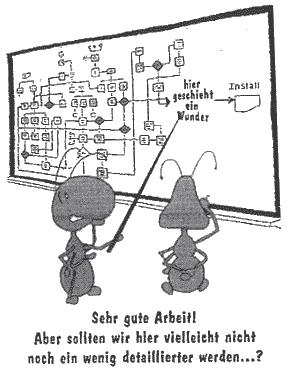
\includegraphics{files/projekt_wunder} \\ 
\medskip
\textit{F�r den Weg den ich hier beschritten habe. Dies ist das einzige was diesen Weg rechtfertigt und die Hoffnung transportiert, dass dies jemals jemand anderer verstehen w�rde.}
\end{center}
}


\pagestyle{plain}

\newpage
\tableofcontents

\newpage
\pagenumbering{arabic}
%\setcounter{page}{1}

\pagestyle{fancy}
\renewcommand{\headrulewidth}{0pt} %
\renewcommand{\footrulewidth}{0.4pt} %
\fancyhead{}{}
%	\fancyfoot{} %


% Auth
%%
%% Qbe SAS SystemDocumentation
%% (C) Copyright 2001-2004 Christian Hofstaedtler
%%
%% $Id: part-01.tex 38 2004-05-12 13:59:31Z ch $
%%

\cChapter{Authentication Server}

Der Authentication Server basiert auf der \index{Application Server}{"Qbe Application Server"} Software, die eine generische Engine zur Verf�gung stellen soll, die folgendes bietet:
\begin{itemize}
\item Ausf�hrung einer sogenannten Applikation f�r \index{HTTP}{HTTP}. \index{Engine}{Engine} und Applikation werden in PHP implementiert, Hintergrunddienste vorzugsweise in \index{Perl}{Perl}, oder auch C/C++.
\item Einfache Einbindung von anderen Systemen in die Applikation.
\item Modularit�t und klare Trennung von Teilkomponenten
\item Transparentes Handling von verschiedenen \index{Grundfunktionen}{Grundfunktionen}, wie Men�\-sys\-tem, SSL, einheitliches Seitenlayout \ldots
\end{itemize}

In der vorhandenen Implementierung sind Engine und Applikation nicht klar voneinander getrennt, da erst in einer sp�ten Projektphase die gro�e Wiederverwendbarkeit aufgedeckt wurde. Daher kann nur eine echte Anwendung (mit einigen Sub-Anwendungen) pro Installation ausgef�hrt werden, die Modularit�t ist ebenfalls teilweise nicht gegeben, wurde aber laufend bis zum Projektende verbessert.


\section{Software-Teile}
\subsection{Verzeichnisstruktur}
Verwendete Verzeichnisse auf dem AuthServer:

\begin{description}
\item[/qbe]
	Qbe Application Software
\item[/qbe-local]
	Lokale Einstellungen f�r Qbe Application Software \\
	Lokal bedeutet, lokal f�r diesen Server -- sind mehrere Server vorhanden (z.B. in einem Cluster) k�nnen Dateien unter diesem Verzeichnis unterschiedlich sein.
\item[/var/lib/mysql]
	\index{MySQL}{MySQL} Database
\item[/var/lib/ldap]
	\index{LDAP}{OpenLDAP} Database (falls vorhanden)
\item[/var/novell]
	Novell \index{eDirectory}{eDirectory} State (falls vorhanden)
\item[/var/lib/nds] 
	Novell eDirectory Database (falls vorhanden)
\item[/import/homes]
	Benutzerverzeichnisse
\item[/import/homes/qbe-systemstate]
	Qbe Application Software Systemstatus
\item[/import/homes/qbe-inetstate]
	Qbe Systemstatus: Modul internet
\item[/import/homes/.status]
	Qbe Application Software Systemstatus (compatibility)
\end{description}

\subsection{Verzeichnisse unter /qbe}
\begin{description}
\item[etc]
	Konfigurationsdateien und Vorlagen f�r automatisch erstellte Systemkonfigurationen.
\item[data]
	Enth�lt tempor�re Daten.
\item[sbin]
	Programme, die die Hintergrunddienste der Applikation implementieren. Perl- und Shell-Skripte, C-Applikationen.\\
	Achtung: keine Ordner - Modulspezifische Programme sollten \\ \verb|qbe-modulname-programmname| benannt werden.
\item[status]
	Enth�lt tempor�re Statusinformationen.
\item[web]
	Dateien der Applikation, die f�r \index{HTTP}{HTTP} ben�tigt werden. \\
	Ideal: nur Unterordner und defines.*.php.
\item[web/htdocs]
	Dateien die den benutzersichtbaren Teil der Applikation bilden. PHP Skripte, Grafiken, \ldots
\end{description}

\subsection{Dienste}

Qbe SAS setzt auf bereits lang existierenden, gut implementierten Diensten auf, diese sind:

\begin{tabular}{|r|l|l|}
\hline
Dienst & Implementation & Daemon \\
\hline
DNS & ISC BIND 9 & named \\
\index{DHCP}{DHCP} & ISC DHCP 3 & dhcpd \\
LDAP & Novell eDirectory 8.7 & ndsd \\
 & OpenLDAP 2 & slapd \\
SQL Datenbank & MySQL 4.1 & mysqld \\
Webserver (+SSL) & Apache 1.3 & apache \\
Versionskontrolle & Subversion 1.0 & mod\_dav\_svn im apache2 \\
\hline
\end{tabular}

Notiz: es ist durchaus m�glich, Qbe SAS mit dem OpenLDAP Server zu verwenden, jedoch wird in der HTL Novell eDirectory eingesetzt, 
da bei Tests in fr�heren Projektstadien es sich abgezeichnet hat, dass der \index{OpenLDAP}{OpenLDAP} Daemon die Last von 1500 Benutzern nicht handlen k�nnte.
Da nach der Umstellung auf Novell eDirectory noch \index{Schemaerweiterungen}{Schemaerweiterungen} dazugekommen sind, m�sste das Schema wieder in eine OpenLDAP kompatible Form gebracht werden. 

Die aktuellen Schemaerweiterungen sind im Anhang ersichtlich.

\section{Konfiguration}

Die Qbe SAS Konfiguration besteht aus mehreren einzelnen Konfigurationsdateien. Diese werden weiter unten ausf�hrlich erkl�rt:

\begin{description}
\item[/qbe/web/defines.php] \index{Application Server}{Application Server} Grundkonfiguration
\item[/qbe/web/defines.app.php] Konfiguration der Anwendung (hier: Qbe SAS)
\item[/qbe/web/defines.local.php] Serverspezifische Einstellungen f�r Cluster Installationen
\item[/qbe/web/defines.security.php] Sicherheitseinstellungen der Anwendung
\item[/qbe/etc/perl/qbesystemconfig.pm] Perl Konfiguration
\item[/qbe/etc/modules/computer/dhcpd.template] Vorlage f�r die \index{DHCP}{DHCP} Konfigurationsdatei
\end{description}

\noindent
Weiters werden einige System-Konfigurationsdateien verwendet:
\begin{description}
\item[/etc/apache/httpd.conf] Apache Konfiguration
\item[/etc/apache/ssl*] SSL Zertifikate f�r den \index{HTTP}{HTTP} Server
\item[/etc/crontab] Zeiteinstellungen f�r \index{cron}{crond}
\item[/etc/dhcp3/dhcpd.conf] Konfiguration des DHCP Servers, wird automatisch neu erstellt
\item[/etc/php4/apache/php.ini] PHP Konfiguration f�r den HTTP Server
\item[/etc/php4/cgi/php.ini] PHP Konfiguration f�r Background Tasks
\item[/etc/samba/smb.conf] Samba (CIFS Server) Konfiguration
\end{description}

\subsection{/qbe/web/defines.php}
\begin{description}
\item[setlocale(LC\_ALL,"de\_AT");] Setzt die Sprache f�r Ausgaben, Zeiformate, usw. in PHP auf de\_AT -- Deutsch (�sterreich)
\item[\$sas\_ldap\_base] Root-Name der LDAP Datenbank. z.B: "o=htlwrn,c=at"
\item[\$qbe\_http\_basepath] Hauptverzeichniss der Qbe AppServer Dateien. Default: "/qbe/web/htdocs"
\item[\$qbe\_http\_server] Voreinstellung des Servernamens. \\
	Default: wird mit \verb|$_SERVER['SERVER_NAME']| automatisch ermittelt
\item[\$qbe\_ssl] SSL serverseitig vorhanden, ja/nein. Default: true
\end{description}

\subsection{/qbe/web/defines.security.php}
Diese Datei enth�lt normalerweise die benutzten Passw�rter (im Klartext) und sollte daher dem Benutzer \verb|qbe|, Gruppe \verb|www-data| geh�ren. Als Rechte sollte nur Benutzer \verb|rw| und Gruppe \verb|r| gesetzt sein.

\begin{description}
\item[\$sas\_mysql\_server] Hostname des MySQL Servers
\item[\$sas\_mysql\_database] Die Datenbank, die f�r Qbe SAS verwendet werden soll
\item[\$sas\_mysql\_user] Benutzername mit allen Rechten auf die Datenbank
\item[\$sas\_mysql\_password] Zugeh�riges Passwort
\item[\$sas\_ldap\_server] Hostname des \index{LDAP}{LDAP} Servers, normalerweise "localhost"
\item[\$sas\_ldap\_adminuser] Benutzername eines Users mit allen Rechten
\item[\$sas\_ldap\_adminpass] Dazugeh�riges Passwort
\item[\$sas\_ldap\_machineuser] Benutzername eines Users mit eingeschr�nkten (nur-Lesen) Rechten
\item[\$sas\_ldap\_machinepass] Dazugeh�riges Passwort
\end{description}

\subsection{/qbe/web/defines.local.php}
In dieser Datei k�nnen alle Werte aus defines.php oder defines.security.php �berschrieben werden. Die Datei ist in der Regel ein symbolic link auf \verb|/qbe-local/web/defines.local.php| und enth�lt keine Eintr�ge.
In Cluster-Konfigurationen wird dort typischerweise die Variable \verb|$qbe_http_globalservername| mit dem wirklichen Servernamen �berschrieben.

\subsection{/qbe/web/defines.app.php}
Dies ist eine Konfigurationsdatei, spezifisch f�r die Applikation (hier: Qbe SAS).

\begin{description}
\item[\$sas\_version] Qbe SAS Versionsnummer
\item[\$sas\_codename] Qbe SAS Codename der aktuellen Version
\item[\$qbe\_http\_globaldomain] DNS-Domain in der die Server eingetragen sind - muss dem PHP Cookie-Domain Setting entsprechen. z.B: "htlwrn.ac.at"
\item[\$qbe\_http\_globalservername] Vollst�ndiger Servername, z.B: \verb|"qbe-auth.".$qbe_http_globaldomain|
\item[\$sas\_samba\_domainsid] Die Samba Domain-SID. \\
	z.B: "S-1-5-21-1021225642-3915188714-2801850423"
\item[\$qbe\_app\_frontpage] PHP-Skript, welches in der Startseite angezeigt wird. Default: leer.
\item[\$qbe\_util\_arp] Pfad zum ARP Programm mit numerischen IP-Adressen. z.B: "/usr/sbin/arp -n "
\end{description}

\section{Applikationsmodule}
Die Applikationsmodule bestehen aus Dateien in diesen Verzeichnissen:
\begin{description}
\item[/qbe/etc/MODULNAME/] Enth�lt modulspezifische Konfigurationsdateien.
\item[/qbe/web/htdocs/modules/MODULNAME/] Haupt-Modulordner, alle ausf�hrbaren Webskripte, Grafiken, etc. liegen hier. Zus�tzlich existiert eine defines.php, die Modulinformationen, Men�beschreibungen und globale Modulfunktionen enth�lt.
\item[/qbe/web/htdocs/modules/MODULNAME/defines.php] Enth�lt die Men�definitionen f�r das Modul und eventuell vorhandene globale Funktionen.
\item[/qbe/web/htdocs/rpc/MODULNAME/] Ausf�hrbare RPC Objekte, diese sollten die sas.inc.php nicht benutzen.
\item[/qbe/sbin/qbe-MODULNAME-...] Ausf�hrbare Hintergrundprogramme
\end{description}

\subsection{core}
\verb|core| stellt die Kernfunktionalit�t des Application-Servers zur Verf�gung. Dem core-Modul geh�ren auch die Hauptkonfigurationsdateien sowie weitere Dateien ausserhalb des Modulverzeichnisses an:
\begin{description}
\item[admin/admin/finger.php] Kann verwendet werden um die Un*x-Details eines Benutzers abzufragen.
\item[admin/index.php] Das Anmeldeformular
\item[admin/logout.php] Abmeldung des Benutzers
\item[graphics/style.css] Stylesheet f�r die Qbe SAS Seiten
\item[graphics/qbe.sas.about.png] Gro�es Qbe SAS Logo f�r die Release-Informationsseite
\item[graphics/qbe.sas.topright.png] Kleines Qbe SAS Logo f�r das Men� rechts oben
\item[index.php] Die Startseite -- eine einfache Page die definierbare Inhalte darstellen kann. (Siehe Konfiguration.)
\item[modules/defines.php] L�dt alle aktiven Module.
\item[sas.inc.php] Master-Include, stellt die gesamte Basisfunktionalit�t (Seitenstart, -ende, Links, Men�, Hilfe, \ldots) zur Verf�gung.
\end{description}

Dateien innerhalb des Modulverzeichnisses:
\begin{description}
\item[about.php] Eine graphisch ansprechende Informationsseite �ber Qbe SAS, Copyright-Informationen.
\item[checklogin.php] Check, ob der Benutzer angemeldet ist, falls nicht, Login und dann Weiterleitung auf Original-URL. Ist ein Qbe SAS Client mit der HTTP Client IP-Adresse registriert, wird dessen Authentifizierung benutzt.
\item[chpass.php] Frontend zum Passwort �ndern, greift auf die User-Provider-Funktion zur�ck.
\item[datenschutz.php] Stellt Informationen �ber den eigenen Benutzer in halbwegs verst�ndlicher Form dar und informiert �ber einige Grunds�tze des Datenschutzes.
\item[lookup.php] Sucht den passenden Provider f�r das \$subject und leitet den Benutzer auf die entsprechende URL.
\item[lookup-helper.php] F�r Popup-Lookups enth�lt dieses File Javascript-Code, um das Original-Formular zu bef�llen.
\item[sendmsg.php] Sendet (ohne Background Task) eine Nachricht an den Qbe SAS Clients des ausgew�hlten Benutzers.
\end{description}

% core bg tasks
Weiters enth�lt das \keyword{core} Modul einige \keyword{Background Tasks}, die sich um den Systemstatus usw. k�mmern.

\begin{description}
\item[/qbe/web/syscheck.pl]
Dieses Perl Skript wird vom \index{cron}{cron} alle 5 Minuten aufgerufen und �berpr�ft, ob die wichtigsten Dienste (\index{sasd}{sasd}, ndsd, mysqld, apache, dhcpd und smbd) laufen, und schreibt mit diesen Informationen die Datei \verb|/qbe/web/sysstate.php|.
Diese \index{sysstate.php}{sysstate.php} wird vom \index{Master Include}{Master Include} eingebunden und ist f�r die Applikationen als Funktion \verb|sysstate()| verf�gbar.

\item[/qbe/web/cron-10min.sh]
Dieses Shell Skript wird vom \index{cron}{cron} alle 10 Minuten aufgerufen und konfiguriert den DHCP neu bzw. meldet Benutzer ohne aktiven Client vom System ab.

\item[/qbe/web/cron-daily.sh]
Dieses Shell Skript wird t�glich vom \index{cron}{cron} aufgerufen und l�scht die importierten EDVO Benutzer aus dem LDAP Directory. Weiters werden die Dateien unter /export/share-free/ gel�scht.
\end{description}

\subsection{redir}
Stellt erweiterte URL-Weiterleitungsfunktionen zur Verf�gung.

Dateien innerhalb des Modulverzeichnisses:
\begin{description}
\item[outside.php] Baut ein iframe mit dem Qbe SAS Template und der Original-URL auf.
\item[ssl.php] Leitet den Benutzer (falls SSL eingeschaltet ist) auf den \index{HTTP-SSL}{HTTP-SSL} Port des Application Servers weiter.
\end{description}


\subsection{ldap}
Providermodul, dass die Authentifizierung und Verwaltung von Benutzern im LDAP Verzeichnis erm�glicht.

Aufgrund anf�nglich nicht modularer Implementierung sind viele Dateien des \verb|ldap|-Modules �ber die alte Verzeichnisstruktur verteilt:
\begin{description}
\item[admin/login.php] Meldet den, in den POST-Variablen \verb|user| und \verb|pass| spezifizierten Benutzer, an und speichert alle relevanten Daten in die \$\_SESSION Variable.
\item[admin/activation.php] Benutzer mit Erst-Passwort werden auf diese Seite umgeleitet, um ihr Passwort zu �ndern. Dabei wird dann auch das Benutzerverzeichnis angelegt.
\end{description}

\subsection{ldif}
Providermodul f�r den Import von Benutzern in den \index{LDAP}{LDAP} Tree.

Dateien im Modulverzeichnis:
\begin{description}
\item[import.php] Importiert \index{Benutzerlisten}{Benutzerlisten} im \index{CSV}{CSV}-Format
\item[import\_passwords.php] Importiert nur die Passw�rter von Benutzerlisten (CSV)
\end{description}

\subsection{computer}
Stellt die Verwaltung der Computer-Objekte und der Notebook-Attribute der Benutzerobjekte zur Verf�gung.

\begin{description}
\item[act.php] Verwaltung bereits existierender Computer Objekte
\item[add-client.php] F�gt ein neues Computer Objekt hinzu
\item[getip.php] Zeigt die aktuelle IP und MAC-Adresse des \index{HTTP}{HTTP} Clients oder von anderen Computern
\item[manage-clients.php] Verwaltung bereits existierender Computer Objekte: Auflistung
\end{description}

Andere Dateien:
\begin{description}
\item[admin/tools/request\_clearance.php] Komplettes Verwaltungsinterface f�r die Notebooks der Benutzer
\end{description}

Als \keyword{Background Task} existiert nur die qbe\_dhcpconf.pl, die vom cron-10min.sh aufgerufen wird, und die statischen DHCP Eintr�ge exportiert.

\subsection{client}
Dieses Modul stellt ausschliesslich RPC-Objekte f�r den Qbe SAS Client zur Verf�gung. 

Die RPC Objekte befinden sich im \verb|/rpc/client| Verzeichnis und sind im Kapitel \ref{chap-csprotocol} dokumentiert. Aliasnamen zur Kompabilit�t mit iLogin v2 $<=$ 2.20 wurden mit Qbe \index{Application Server}{Application Server} Version 0.91 entfernt. Alte Clients k�nnen sich daher nicht mehr anmelden.

\begin{description}
\item[index.php] Auswahlhilfe f�r die Qbe SAS Client Downloads
\item[update.php] Wertet den GET-Parameter "ver" aus und sendet entweder \index{Statuscode}{Statuscode} 404 (Aktuelle Version ok) oder die neue Installations-Datei
\item[version.php] Enth�lt die aktuelle und die minimal notwendige Version des SAS Clients
\end{description}

\subsection{filexs}
Dieses Modul stellt im Webinterface eine M�glichkeit zur Verf�gung, die Dateien im eigenen Benutzerverzeichnis zu verwalten. Folgende Aktionen sind m�glich: \index{fileget}{Datei herunterladen} (fileget), Datei abspeichern (fileput), L�schen (unlink bzw. rmdir), Umbenennen (rename) -- alle Aktionen werden im \index{setuid}{setuid}/setgrp-Bereich des jeweiligen Benutzers ausgef�hrt. Au�erdem kann auf die "free"- und "alle"-Freigaben zugegriffen werden.

Alle zugeh�rigen Dateien befinden sich in den entsprechenden Verzeichnissen.

Dateien im Modulverzeichnis:
\begin{description}
\item[index.php] Listet das ausgew�hlte Verzeichnis auf.
\item[inc.php] Modul-Include
\item[act.php] Frontend f�r den qbe-filexs Background-Task.
\item[xfer-get.php] Frontend f�r den qbe-filexs BgTask: Dateidownload (fileget)
\item[xfer-put.php] Frontend f�r den qbe-filexs BgTask: Dateiupload (fileput)
\end{description}

Das filexs Modul enth�lt nur den Pseudo-\keyword{Background-Task} "\index{qbe-filexs}{qbe-filexs}" (ein \index{setuid}{setuid} root-Binary), welcher sich um die eigentlichen Dateizugriffe k�mmert. Damit liegen alle Sicherheitsprobleme und die Access-Control in diesem Background Task.

\begin{Verbatim}
ch@xtc:/qbe/sbin -> ls qbe-filexs
-r-sr-sr-x    1 root     root         7643 Dec 19 13:10 qbe-filexs

Aufrufparameter:
/qbe/sbin/qbe-filexs user group action file [file2]
                     |    |     |      |    |
                     |    |     |      |    Ein zweiter Dateiname
                     |    |     |      Dateiname    
                     |    |     Die auszuf�hrende Aktion
                     |    Gruppenname oder "-"
                     Benutzer unter dem die Aktion ausgef�hrt
                     werden soll.
\end{Verbatim}


\subsection{changelog}
Stellt die F�hrung des System-�nderungsprotokolls durch Administratoren zur Verf�gung -- nur Administratoren k�nnen das ChangeLog einsehen. Die Eintr�ge (bestehend aus Datum, Benutzername und Logtext) werden in der SQL-Tabelle \index{sas.changelog}{sas.changelog} gespeichert.

Dateien im Modulverzeichnis:
\begin{description}
\item[prettyprint.php] Gibt das komplette ChangeLog als eine HTML Tabelle ohne weitere Stilinformationen aus.
\item[latex.php] Gibt das komplette ChangeLog als \LaTeX longtable aus.
\item[index.php] Listet das ChangeLog innerhalb des Templates auf und erm�glicht Administratoren die Eingabe von neuen Eintr�gen.
\end{description}

\subsection{nagios}
Ein typisches \index{Custom-Modul}{Custom-Modul}, stellt f�r die Startseite (die Verwendung ist getrennt zu konfigurieren) Inhalt (Nagios �bersichtsbild) und einen Reverse Proxy zur Verf�gung.

Dateien im Modulverzeichnis:
\begin{description}
\item[frontpage.php] Custom Inhalt f�r Startseite
\item[.htaccess] Konfiguriert einen Reverse Proxy, basierend auf mod\_rewrite, f�r das Bild dass die Nagios-Software erstellt
\end{description}

\subsection{help}
Implementiert das Hilfesystem. Die Seiten werden mit \verb|index.php| dargestellt (welches nur im PopUp-Modus arbeitet), die einzelnen Hilfeseiten werden unter \verb|topics| abgelegt.

\placefigx{scr-sas-help}{Screenshot des Hilfe-Fensters}{width=9cm}

\subsection{dev}
Zeigt einige Funktionen der Qbe AppServer Engine, mit Codebeispielen. Legt keine Men�eintr�ge an.

Dateien im Modulverzeichnis:
\begin{description}
\item[demo.php] Zeigt Codebeispiele f�r gebr�uchliche Funktionen.
\item[masterinc.php] Zeigt Funktionen aus dem \index{Master Include}{Master Include} File.
\end{description}

\subsection{internet}
Mit diesem Modul wird die Integration mit dem Qbe SAS Proxy (Kapitel \ref{chap-proxy}) realisiert. Am Authentication Server k�nnen die einzelnen Klassen oder Gruppen freigeschaltet werden. Das Modul f�hrt �ber jede Internetstatus-�nderung Protokoll, inklusive Zeit und IP-Adresse, welches dann durch Administratoren einsehbar ist. Damit kann man relativ leicht herausfinden, ob das Passwort eines Lehrers bekannt geworden ist.
\placefigx{scr-sas-inetlock}{Internetzugangskontrolle}{width=10cm}

Dateien im Modulverzeichnis:
\begin{description}
\item[index.php] Stellt eine grafisch ansprechende Ansicht �ber die Klassen und Gruppen dar, siehe Bild \ref{fig:scr-sas-inetlock}
\item[save.php] Validiert und speichert den neuen Internetstatus f�r Klassen bzw. Gruppen
\item[pconly.php] Erlaubt es einzelne Computer freizuschalten
\item[log-inetsave.php] Stellt die vergangenen Internetstatus�nderungen in einer Tabelle dar
\item[stats-traffic-class.php] Summiert das Trafficvolumen auf Anfrage klassenweise
\item[stats-traffic-overall.php] Zeigt das gesamte Trafficvolumen aufgesplittet nach Abteilungen auf
\item[stats-traffic-overall.chart.php] Grafikausgabe f�r \verb|stats-traffic-overall.php|
\end{description}

\subsection{rfid}
Implementiert die Elektronische Inventarverwaltung, ein weiteres Projekt der HTBLuVA Wiener Neustadt.

\subsection{sis}
Enth�lt die Implementierung des Schul-Informations-Systems, ein weiteres Projekt der HTBLuVA Wiener Neustadt.


%% *eof*


% Proxy
%%
%% Qbe SAS SystemDocumentation
%% (C) Copyright 2001-2003 Christian Hofstaedtler
%%
%% $Id: part-02.tex 36 2004-05-12 13:04:34Z ch $
%%

\cChapter{Proxy -- Internetgateway}
\label{chap-proxy}

Der Qbe SAS Proxy stellt die Verbindung zum Internet her. Alle ausgehenden Verbindungen passieren den \index{Proxy}{Proxy} -- teilweise durch Application Proxies oder IP-Forwarding. Zugriffe werden zentral �ber Qbe SAS kontrolliert und protokolliert.
Der Proxy wird fast ausschliesslich mit Standard OpenSource Software implementiert.

\section{Software}
Folgende Standardsoftware wird verwendet:

\begin{itemize}
\item Debian GNU/Linux woody oder OpenBSD 3.2+ oder FreeBSD 4.x
\item Linux Kernel 2.4.18+ 
\item Squid Cache 2.4-STABLE oder 2.5-STABLE -- \index{HTTP}{HTTP} Proxy
\item Frox -- FTP Proxy
\item Perl 5.8 und Module Net::LDAP, File::Tail, DBI, MySql
\item ISC BIND 9 -- DNS
\end{itemize}

Der Proxy l�dt ein Modul, welches die Benutzerauthentifizierung �berpr�ft. Zus�tzlich l�uft nur ein \index{Perl}{Perl-Skript}, das sich mit dem Volumenaccounting besch�ftigt. Das Skript und das Modul werden �blicherweise in \verb|/qbe/sbin/| abgelegt und k�nnen ggf. mit \index{rsync}{rsync} vom AuthServer synchronisiert werden. 


Notiz: Es ist nicht notwendig eine LDAP-Benutzerauthentifizierung f�r das System (Stichwort \index{PAM}{PAM}) einzurichten. 
Idealerweise gibt es auf dem Qbe Proxy nur Systemaccounts und einen Systemverwalter (nicht \verb|root|). 
\verb|root| sollte sich (wie auch am Application Server) nicht �bers Netzwerk anmelden k�nnen.

\section{qbe-proxy-squidlog.pl -- Auswertung der Squid Cache Logs}
Das Perlskript liest die Squid-Logdatei kontinuierlich aus und wertet die Eintr�ge aus, interne Zugriffe werden dabei ignoriert. Die Datentransfergr��e wird (pro Client-IP) im RAM abgespeichert. 
Alle 5 Minuten werden die Daten im RAM in die \index{MySQL}{MySQL-Tabelle} \index{sas.trafficlog}{sas.trafficlog} gespeichert. 
Am AuthServer werden diese Daten dann zusammengez�hlt und in die \index{LDAP}{LDAP-Datenbank} hinzugef�gt. Traffic, der nicht einem Benutzer zugeordnet werden kann, wird beim \verb|nobody|-User dazugez�hlt. F�r eine IP-basierende-Auswertung werden die Daten in eine getrennte Tabelle \verb|sas.trafficip| gespeichert. Weiters kann am AuthServer eine Grafik �ber den Traffic-Verlauf erstellt werden.

\medskip

Tabellenaufbau:
\begin{lstlisting}[language=sql]
CREATE TABLE trafficlog (
  ip varchar(60) NOT NULL default '',
  traffic bigint(20) default NULL,
  KEY client (ip)
) TYPE=MyISAM;

CREATE TABLE trafficip (
  ip varchar(20) NOT NULL default '',
  traffic bigint(20) NOT NULL default '0',
  PRIMARY KEY  (ip)
) TYPE=MyISAM;
\end{lstlisting}

Ein typischer, tempor�rer Eintrag:
\begin{lstlisting}[language=sql]
INSERT INTO trafficlog VALUES ('10.3.5.1',135084);
INSERT INTO trafficip VALUES ('10.1.40.1',8991453419);
\end{lstlisting}

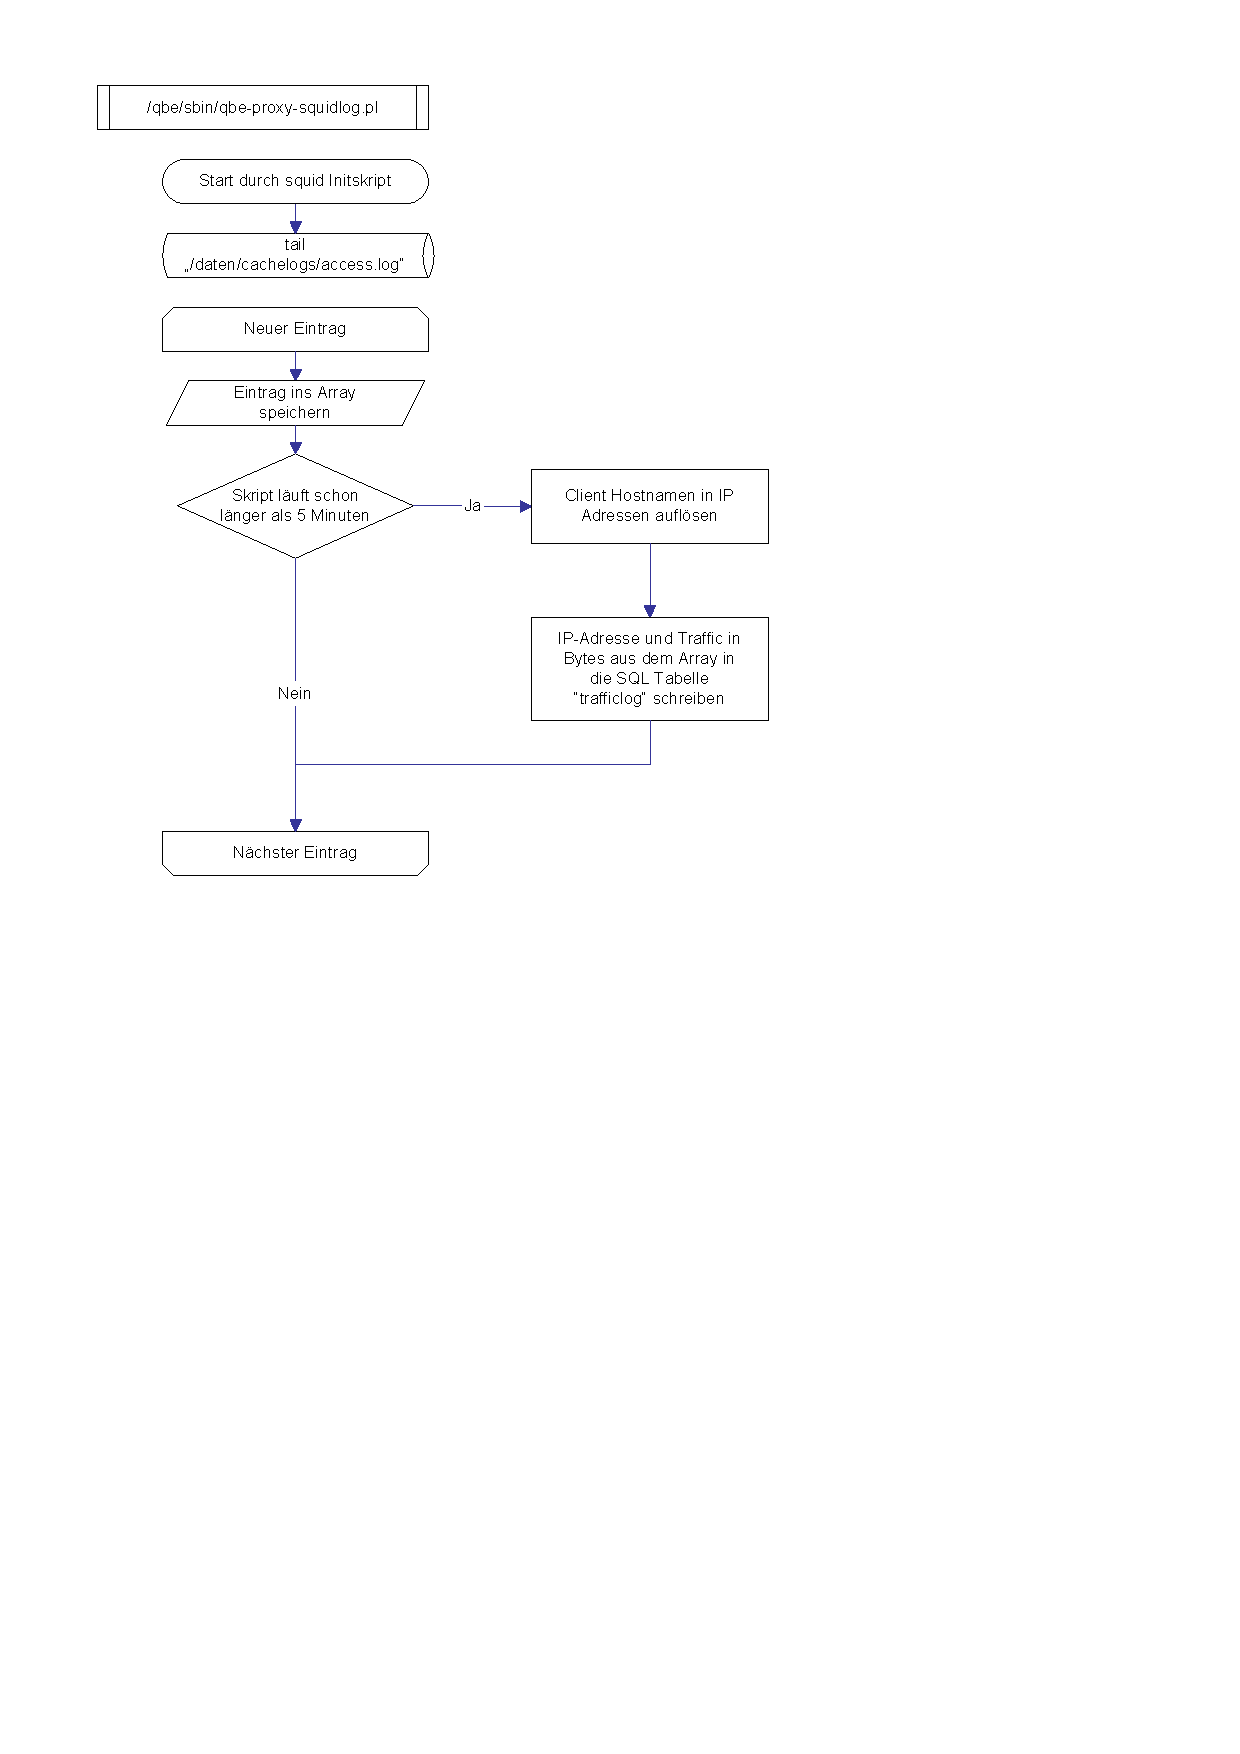
\includepdf[pagecommand={}]{files/flow-qbe-proxy-squidlog.pdf}

\subsection{Grafik-Auswertung nach Benutzern}
Am Authentication Server wird jede Stunde einmal das Skript /qbe/sbin/qbe\_trafficview.pl aufgerufen. Dieses aggregiert die Daten aus dem LDAP und kopiert die Daten pro Benutzer in die Tabelle \verb|sas.trafficview|. Die Tabelle wird im UI mittels /modules/internet/stats-traffic-overall ausgewertet und als Balkendiagramm je Abteilung dargestellt.

\begin{lstlisting}[language=sql]
CREATE TABLE trafficview (
  userid varchar(10) NOT NULL default '',
  traffic bigint(20) NOT NULL default '0',
  abt varchar(5) NOT NULL default ''
) TYPE=MyISAM;
\end{lstlisting}

Ein Beispieleintrag:
\begin{lstlisting}[language=sql]
INSERT INTO trafficview VALUES ('cb',1123132,'Adm');
\end{lstlisting}

\placefig{scr-inettraffic}{Graphische Auswertung}
\clearpage

\section{Zugriffssteuerung f�r Squid Cache}
Fr�here Qbe SAS Systeme setzten auf ein Perlskript welches regelm��ig die aktuell angemeldeten Benutzer abgefragt und in eine Datei geschrieben hat. Um die damit verbundenen Probleme zu l�sen, wird jetzt ein Modul in den Squid Cache geladen. Das Modul heisst "ip\_ldap" und wird als "external acl" eingetragen.

%Es wird eine Verbindung zum AuthServer/LDAP aufgebaut und eine Liste aller freigeschalteter Benutzer (daher Filter $(|(inetStatus=0) (inetStatus=7))$) abgerufen. Die Eintr�ge werden auf G�ltigkeit und Vorhandensein der Attribute \verb|loggedonHost| und \verb|loggedonMac| �berpr�ft. Eintr�ge, die diese Kriterien erf�llen werden im Format "\verb|loggedonHost|/32" in die Datei \verb|/qbe/data/squid.include| geschrieben.
%Um Fehlermeldungen des Squids zu vermeiden, wenn keine Benutzer angemeldet sind, wird zus�tzlich der harmlose Eintrag 127.0.0.1/32 geschrieben.

%Anschlie�end wird der \index{Squid}{Squid-Cache} angewiesen, die Konfiguration neu einzulesen. Ablaufdiagramm auf der n�chsten Seite. 
%%dazu siehe Abb. \ref{fig:flow-qbe-proxy-squidacl}

%\placefig{scr-proxyaccessdenied}{Fehlermeldung vom Proxy bei keiner Anmeldung}
%\clearpage
%%\placefig{flow-qbe-proxy-squidacl}{Ablaufdiagramm qbe-proxy-squidacl.pl}
%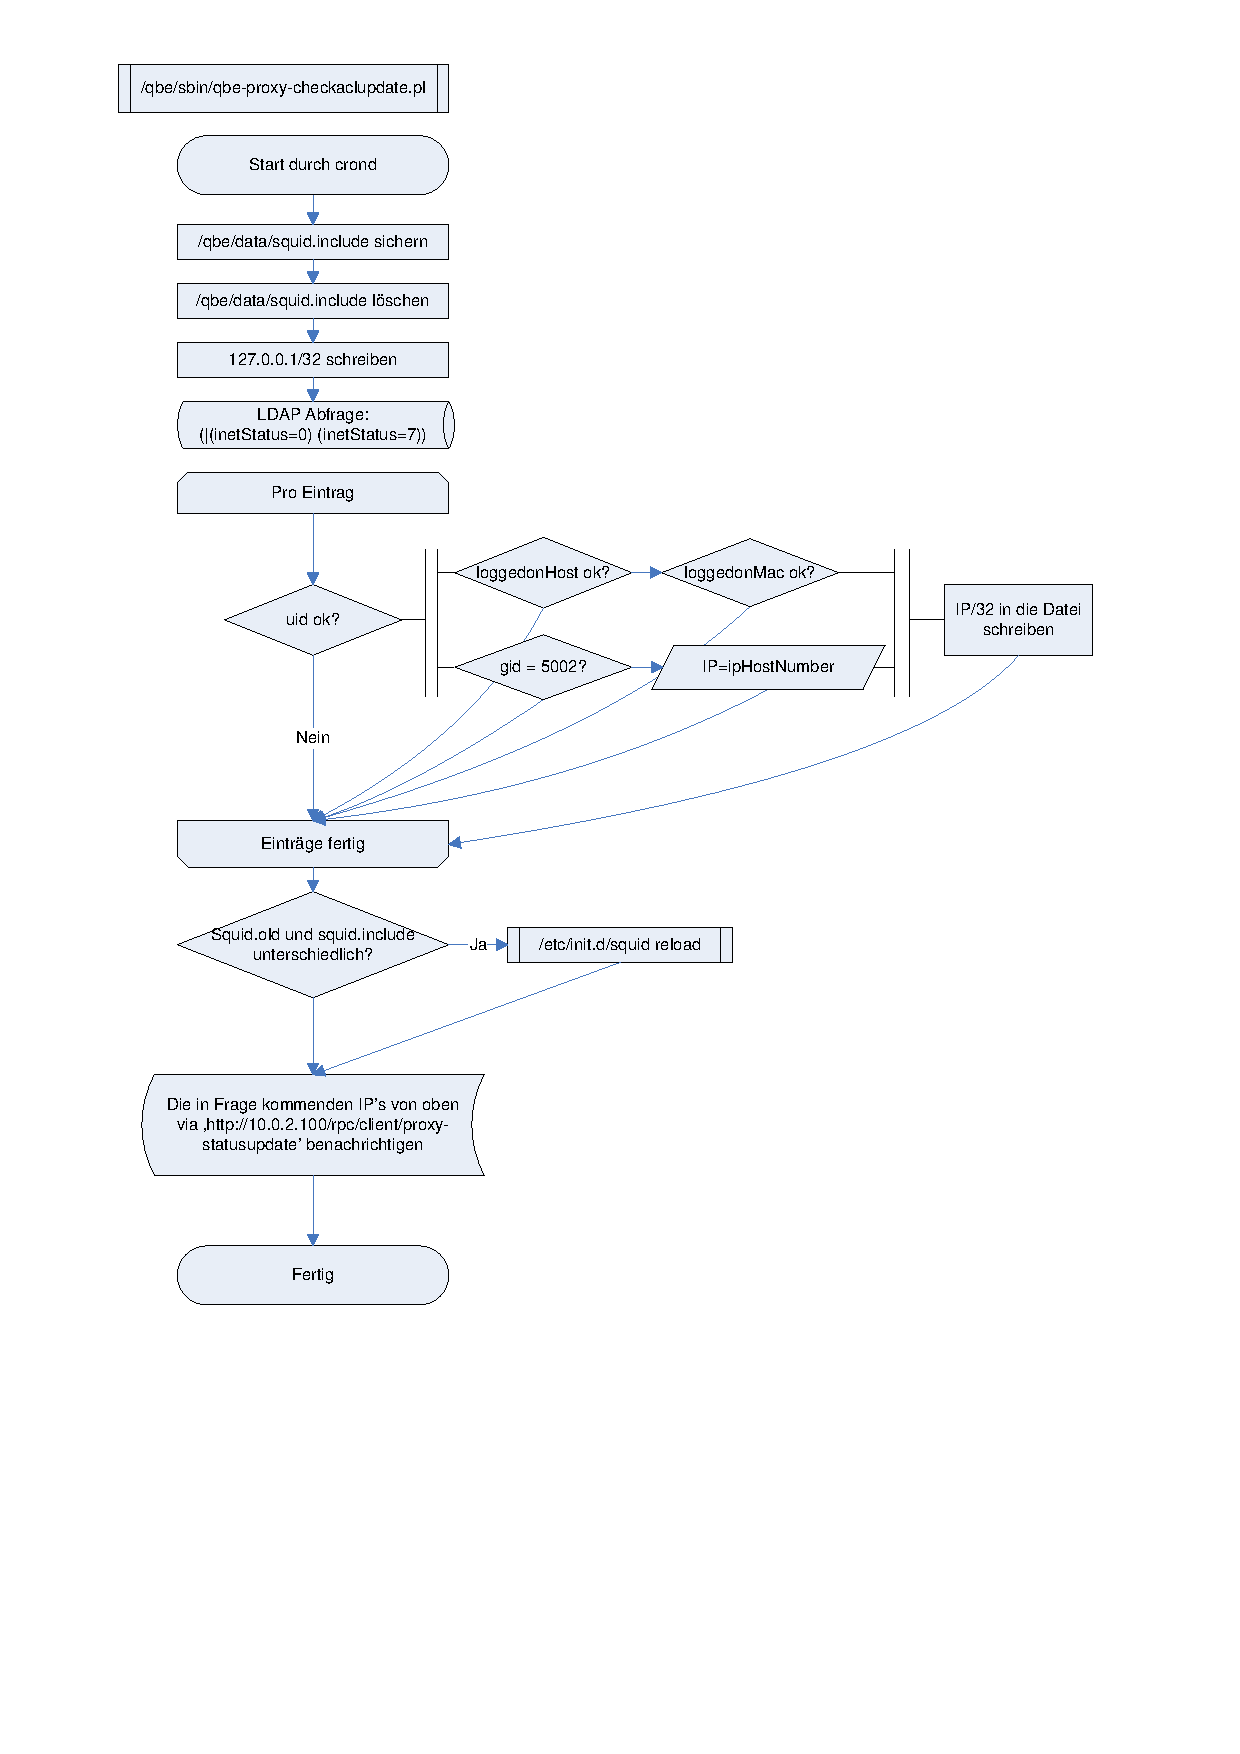
\includepdf[pagecommand={}]{files/flow-qbe-proxy-squidacl.pdf}
%

\section{�nderungen an der System-Konfiguration}

Es werden hier kurz die notwendingen �nderungen an der Standardkonfiguration eines Debian-Systems beschrieben.

\subsection{Squid: Initskript}
Das Initskript des Squid Cache daemons \verb|/etc/init.d/squid| muss angepasst werden, um \verb|qbe-proxy-squidlog.pl| entsprechend zu starten bzw. zu beenden.

Ans Ende der \verb|start()|-Routine geh�rt folgende Zeile:
\begin{lstlisting}
# Qbe SAS Proxy
/qbe/sbin/qbe-proxy-squidlog.pl&
# END
\end{lstlisting}

An den Anfang der \verb|stop()|-Routine muss folgendes hinzugef�gt werden:
\begin{lstlisting}
# Qbe SAS Proxy
killall "qbe-proxy-squidlog.pl"
# END
\end{lstlisting}

\subsection{Squid: ACL}
Um den Clients die Benutzung des Squid Caches zu erlauben, muss in der \verb|/etc/squid/squid.conf| ein \index{ACL}{ACL-Eintrag} hinzugef�gt werden:
\begin{lstlisting}
# angemeldete Benutzer
external_acl_type ldapacl ttl=45 \%SRC \%IDENT /usr/lib/squid/ip_ldap
acl proxy-users external ldapacl
\end{lstlisting}

Anschliessend mu� diese ACL in der \verb|allow|-Klasse eingetragen werden:
\begin{lstlisting}
http_access allow proxy-users
\end{lstlisting}

\section{WebSense EIM}
Soll der "WebSense Employee Internet Manager" installiert werden (der f�r �sterreichische Schulen zum Zeitpunkt des Schreibens nur einer kostenlosen Registrierung bedarf), muss mindestens Squid 2.5-STABLE verwendet werden. F�r Debian \index{Debian}{woody} ist daher ein eigenes Paket notwendig.

Mit einem kleinen Patch kann das sid-Sourcepaket (hier: 2.5.4-3) verwendet werden. Es sind dann noch zwei Pakete aus unstable zu installieren, diese sind jedoch nicht plattformabh�ngig und funktionieren ohne Modifikation.

\lstinputlisting[language=C]{files/squid-2.5.4-woody.patch}

\section{Firewall Hinweis}
Es soll hier ein Hinweis auf \verb|iptables| (bzw. \verb|ipf| oder \verb|pf| unter FreeBSD/OpenBSD) gegeben werden, mit denen eine Firewall-Funktionalit�t aufgebaut werden kann. Dies ist dringend zu empfehlen. Es sollten auch keine anderen Dienste auf dem Qbe SAS Proxy laufen (z.B. Webserver, MySQL...) da diese ein nicht einsch�tzbares Sicherheitsrisiko beherbergen k�nnen.

\section{Ideen f�r die Zukunft, bessere Skalierbarkeit}
Die in dieser Version eingesetzte ACL-Kontrolle �ber eine Datei funktioniert zwar, f�hrt jedoch teilweise zu obskuren Problemen. 
Da der Squid die ACL-Datei nur bei einem SIGHUP neu einliest, und dabei leider manchmal offene Verbindungen (warum er dies tut, ist mir unbekannt) unterbricht, w�re eine z.B. MySQL-basierende ACL besser. 
Dazu muss jedoch der Squid entsprechend erweitert werden und die Login/Logout Skripte am Authentication Server angepasst werden. 
�nderungen am Internet-Status der Benutzer k�nnte man mit einem LDAP-Event abfangen und damit die Datenbank aktualisieren.

Eine andere M�glichkeit w�re das \index{Squid}{Squid} external-acl API zu verwenden. 
Dann l�uft ein kleines Programm, dass nur mit dem \index{LDAP}{LDAP} Server spricht, sobald der squid einen Benutzer authentifizieren muss. 
Die Cache-Vorhaltezeit des Ja/Nein-Zustandes ist dann im Squid selbst konfigurierbar.

%% *eof*


% WebServer
%%
%% Qbe SAS SystemDocumentation
%% (C) Copyright 2001-2004 Christian Hofstaedtler
%%
%% $Id: part-03.tex 2 2004-03-10 08:40:26Z ch $
%%

\cChapter{Webserver Integration}
Qbe SAS ist vorbereitet um in Kooperation mit einem getrennten Webserver die Webseite der Institution und die pers�nlichen Seiten der Systembenutzer anzuzeigen.

\section{Software}
Folgende Standardsoftware wird verwendet:

\begin{Verbatim}
Debian GNU/Linux woody, RedHat Linux, alternativ FreeBSD/OpenBSD
Apache HTTP Server 1.3 oder 2.0
NFS Client
\end{Verbatim}

\section{Konfiguration}
Da keine spezielle Software verwendet wird, beschr�nkt sich die Konfiguration auf das NFS Filesystem und den Apache Webserver.

Notiz: Es ist nicht notwendig eine LDAP-Benutzerauthentifizierung einzurichten. Idealerweise gibt es auf dem Webserver nur Systemaccounts und einen Systemverwalter (nicht \verb|root|). \verb|root| sollte sich nicht remote anmelden k�nnen.

\subsection{NFS}
Datei \verb|/etc/fstab| muss um folgenden Eintrag (in einer Zeile) erg�nzt werden:

\begin{Verbatim}
10.0.2.10:/export/homes /import/homes           nfs     rw,soft,
timeo=60,async,nodev,noexec,nouser,nosuid 0 0
\end{Verbatim}

Dies wei�t das System an, beim Neustart automatisch das Filesystem mit den Benutzerverzeichnissen via NFS vom AuthServer (hier: 10.0.2.10) zu importieren. Zus�tzlich werden einige Parameter gesetzt die die Geschwindigkeit und Sicherheit positiv beeinflussen.

\subsection{Apache httpd}
In der Apache Konfigurationsdatei \verb|httpd.conf| muss folgendes sinngem�� hinzugef�gt werden (Beispiel f�r Apache 1.3):
\begin{Verbatim}
LoadModule userdir_module     modules/mod_userdir.so

<IfModule mod_userdir.c>
    UserDir disabled root
    UserDir /import/homes/*/web
</IfModule>
<Directory /import/homes/*/web>
    AllowOverride All
    Options Indexes Includes
    Order allow,deny
    Allow from all
</Directory>
\end{Verbatim}

Soll auch die Institutsseite am AuthServer abgelegt werden, kann diese im Benutzerverzeichniss des Benutzers "`web"' geschehen. Dazu muss zus�tzlich im \verb|httpd.conf| eingetragen werden:
\begin{Verbatim}
DocumentRoot "/import/homes/web"
\end{Verbatim}


%% *eof*


% iLogin
%%
%% Qbe SAS SystemDocumentation
%% (C) Copyright 2001-2004 Christian Hofstaedtler
%%
%% $Id: part-04.tex 20 2004-05-03 15:41:20Z ch $
%%

\cChapter{Qbe SAS Client}

\section{Systemanforderungen}

Qbe SAS Client soll prim�r auf Clientsystemen mit Betriebssystem Windows 2000 und/oder Windows XP Professional laufen. Wenn m�glich soll nur ein kleiner Teil f�r den Benutzer sichtbar sein (Anmeldung, Statusabfrage und Abmeldung) - die Funktion des Systems sollte nicht weiter in den Vordergrund ger�ckt werden. Ebenfalls soll der gesamte Clientteil nur �ber einen definierten minimalen Befehlssatz mit dem Qbe Auth Server kommunizieren und keine direkten LDAP API Aufrufe durchf�hren um maximale Portabilit�t (m�glicherweise auch von LDAP weg) zu erreichen. Bestimmte Fehler am Client sollen nicht die F�higkeit der Kommunikation mit dem Qbe Auth Server beeintr�chtigen; Netzwerk-Disconnects sollen (besonders auf Laptops) transparent behandelt werden.

\section{Betriebsarten}

Qbe SAS Client �bernimmt die Authentifizierung des Benutzers der einen beliebigen Client PC im Netzwerk benutzen m�chte. Dazu kann es in zwei verschiedenen Modi verwendet werden:

\begin{description}
\item[Network only]
Qbe SAS Client authentifiziert den Benutzer nur gegen�ber dem Server. Der Benutzer gibt seinen Benutzernamen und Passwort getrennt ein.
\item[System Logon]
Qbe SAS Client authentifiziert den Benutzer sowohl gegen�ber dem Client als auch dem Server - bereits beim anmelden an die Windows Workstation. Bei Bedarf wird ein lokaler Benutzer angelegt, und bei der Abmeldung wieder gel�scht.
\end{description}

\subsection{Serversuche}

Der zu benutzende Server wird ausschlie�lich per DNS gefunden. Standard\-m��ig benutzt Qbe SAS Client den Servernamen "qbe-auth". Die Aufl�sung des Namens in eine IP Adresse wird vom Betriebssystem durchgef�hrt - Vorraussetzungen daf�r sind:
\begin{itemize}
\item DNS-Server l�uft und ist richtig konfiguriert \\
	("qbe-auth" ist als A-Record eingetragen.)
\item Die Workstation kann den DNS-Server erreichen, und fragt mit dem richtigen Domainsuffix an. Die richtige Konfiguration der Workstation wird vorzugsweise mittels DHCP erreicht.
\end{itemize}

In der aktuell vorhandenen Version besteht keine M�glichkeit den anf�nglichen Servernamen zu �ndern. Geplant ist eine eigene DHCP-Option die vom Qbe SAS Client ausgelesen werden kann - Vorraussetzung daf�r w�re, dass die Workstation die IP-Stack Konfiguration vom DHCP-Server bekommt.

\begin{Verbatim}
; DNS-Beispieleintrag:
qbe-auth.htlwrn.ac.at.	IN	A		10.0.2.100
\end{Verbatim}

 
\subsection{Einzelteile}

Der Qbe SAS Client ist ein komplexes System, dass aus vielen kleineren Teilen besteht:

\begin{tabular}{|l|l|l|}
\hline
Teilsystem & Dateiname \\
\hline
Network Authentication Service & QbeSvc.exe \\
 & QbeSAS.dll \\
System Logon & QbeGina.dll \\
Statusanzeige & QbeTray.exe  \\
UI Components & iLogin.hta \\
& startup.hta \\
& Q.ico \\
COM API	& iLoginCOM.dll	\\
Einstellungen & iLogin.reg \\
Installation & ServicePack.exe \\
 & netQbe.inf \\
 & QbeNDI.exe \\
\hline
\end{tabular}

Qbe SAS Client kann bereits mit nur dem installiertem "qbesvc.exe" im "Network only" Modus betrieben werden - f�r den "System Logon" Modus bzw. f�r eine benutzerfreundliche Umgebung sollte der Client vollst�ndig installiert werden.


%\begin{center}
%	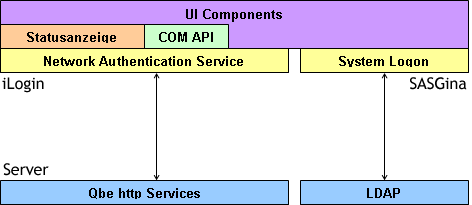
\includegraphics[width=1.00\textwidth]{files/pic-03-beziehungsdiagramm}
%\end{center}
\placefig{pic-03-beziehungsdiagramm}{Beziehungsdiagramm Qbe SAS Client/Server}


Im Beziehungsdiagramm wird deutlich, dass der Network Authentication Service alle grundlegenden Dienste f�r den iLogin Client zur Verf�gung stellt. Wird der System Logon Mode benutzt, wird ein zus�tzlicher Teil systemwichtig -- die SASGina. Dieser wird in das Windows Login eingebunden, und �bernimmt die Windows Anmeldung, LDAP Benutzer�berpr�fung und Datenspeicherung.

\subsubsection{Network Authentication Service}

Dieser l�uft als Windows-Dienst und implementiert sowohl einen HTTP-SSL Client f�r die Kommunikation mit dem Qbe-Auth Server, als auch einen HTTP Server (auf TCP/IP Port 7666) der die Interaktion mit dem Benutzer erm�glicht und Teile des Authentifizierungshandshakes abarbeitet. Auf den Network Authentication Service kann mit einem normalen Webbrowser zugegriffen werden, speziell wurde dies aber f�r den Internet Explorer (bzw. f�r die Microsoft HTML Engine) entwickelt und optimiert, da die restlichen Benutzerinterface-Teile auf der Microsoft HTML Engine aufsetzen. 

Alle weiteren Teile kommunizieren ausschlie�lich mit dem Network Authentication Service der alle relevanten Daten �ber den Benutzer im Speicher h�lt - diese Daten werden regelm��ig vom Server aufgefrischt.

Der HTTP Server erm�glicht es dem Server au�erdem, bestimmte Parameter (Benutzername, Servername, Letzte Verbindung, ...) abzufragen sowie Programme auszuf�hren (etwa um einen Drucker zu installieren). Dies wird durch eine Abfrage der IP-Adresse gesch�tzt.

\subsubsection{COM API and Authentication Helper}

Das COM API erm�glicht es auf den Network Authentication Service per Microsoft COM (ActiveX) zuzugreifen. Gleichzeitig erlaubt es eine Speicherung der Benutzerdaten (Username und Passwort) in der Registry um die Anmeldung zu beschleunigen. Wird iLogin im System Logon oder Single Sign On Mode betrieben, holt das COM API den Benutzernamen und Passwort vom Windows System. \\


\subsubsection{Statusanzeige}

Die Statusanzeige besteht aus einem Windows System Tray Symbol dass den aktuellen Internetstatus signalisiert, wichtige Ereignisse dem Benutzer mitteilt und schnellen Zugriff auf die iLogin Statusseite und Anmeldung erlaubt.
F�r die Statusseite und Anmeldung werden die "UI Components" gestartet.
Energie-Events werden vom iLogin Tray Symbol behandelt. Bei einem kritischen Energieereignis (Standby/Ruhezustand) wird versucht eine Abmeldung durch den Network Authentication Service zu erreichen. 30 Sekunden nach dem Aufwachen wird eine transparente Verbindungswiederherstellung eingeleitet.

\subsubsection{UI Components}

Die sogenannten UI Components bestehen lediglich aus Beschreibungsdateien f�r \href{http://msdn.microsoft.com/workshop/author/hta/overview/htaoverview.asp}{Microsoft HTA Applikationen}, die auf den http Server im Network Authentication Service verweisen.

\placefig{scr-win32client}{Screenshot Qbe SAS Client unter Windows}

\subsubsection{Einstellungen}

Qbe SAS Client installiert bei der Anmeldung einige Standardeinstellungen (z.B. Proxykonfiguration), die direkt aus der Datei "iLogin.reg" kommen. Diese wird mit Hilfe vom Windows Registrierungseditors automatisch in die Registry importiert.

\subsubsection{Update}
Da der Client bei jeder Anmeldung die Versionsnummer an den Server sendet, k�nnen alte/problematische Client-Versionen einfach ausgeschlossen werden. Clients die den Statuscode \verb|404 - Not found| erhalten, sollten keine weitere Anfrage an den Server schicken.

Neuere Windows Clients (ab 2.01) stellen die Benutzerschnittstelle erst nach einer Anfrage an den Server dar. Damit kann ein Update des Clients erzwungen werden. Workstations mit HDGUARD werden am Client abgefragt und das Zwangupdate wird �bersprungen.


\section{Installation}
\subsection{Qbe SAS Client}
Das Setup bietet keine Optionen an und installiert alle Dateien nach \%SystemRoot\%/System32/Qbe/Setup. Die Reihenfolge:
\begin{itemize}
\item[-] .NET VM wird gegebenenfalls heruntergeladen und installiert.
\item[-] \%SystemRoot\%/System32/Qbe/Setup wird komplett gel�scht.
\item[-] PFC wird in das System kopiert und ausgef�hrt (siehe unten)
\item[-] Dateien von fr�heren Versionen die nach \%SystemRoot\%/System32 und \%ProgramFiles\%/iLogin installiert wurden werden gel�scht
\item[-] Alle Dateien werden nach \%SystemRoot\%/System32/Qbe/Setup kopiert
\item[-] Windows NDI installiert den Qbe SAS Client als NetService-Komponente
\item[-] QbeGina wird nicht automatisch installiert/upgedated
\end{itemize}

\subsection{PFC}
Qbe "Pre-Flight-Check" ist eine .NET Anwendung (ClientSource/SetupPFC) die vor der eigentlichen Installation ausgef�hrt wird und folgende Tasks erledigt:
\begin{itemize}
\item vorherigen Versionen von QbeSvc, QbeTray, iLogin, etc. schliessen
\item QbeSvc aus der Registry entfernen
\item HTA-Ausf�hrungsschicht (MSHTA) beenden
\item Windows Service-Pack �berpr�fen und ggf. das aktuelle Service Pack installieren
\end{itemize}

\subsection{Wizard}
Es ist ein Installationswizard geplant der den Benutzer durch die Schritte Client Installation, Computerkonfiguration, Account Aktivierung und Netzwerkkarte registrieren f�hrt. Dieser wurde bereits in .NET angefangen, ist jedoch nicht fertig. (Projektverzeichnis ClientSource/Wizard)

\subsection{System-Updates}

Der SAS Client (f�r Windows) ben�tigt Windows 2000 oder XP mit installiertem .NET Framework. Das aktuelle Servicepack auf den Zielsystemen ist nicht zwingend erforderlich, w�re aber von Vorteil.
Das Client Setup pr�ft vor der eigentlichen Client-Installation ob das .NET Framework und die Microsoft C++ 7.1 Runtimes vorhanden ist - wenn nicht wird beides heruntergeladen und installiert.

\subsubsection{.NET Framework}
F�r das .NET Framework wird mittels Registry-Key die Installation �berpr�ft, andernfalls wird das Setup heruntergeladen und gestartet. Kein Setup-Neustart.

\begin{Verbatim}
URL: http://qbe-auth.htlwrn.ac.at/login/dotnetfx.exe

ch@xtc:/qbe/web/htdocs/login -> ls -la dotnetfx.exe
-rw-rw-r--  ch   sysops   24277024 Mar  4  2003 dotnetfx.exe
\end{Verbatim}	

\subsubsection{Service-Pack}
F�r das Service-Pack wird die NSI-Anwendung (ClientSource/Setup/ServicePack.nsi) gestartet die dann vom AuthServer das ServicePack herunterl�dt und installiert.
Die ServicePack Installationsdateien dazu liegen am AuthServer im /login/ Verzeichniss.
\begin{Verbatim}
URL: http://qbe-auth.htlwrn.ac.at/login/servicepack.php?ver=5.0

ch@xtc:/qbe/web/htdocs/login -> ls -la service*exe
-rwxrw-r--  ch   sysops   135945992 Jun 20  2003 servicepack-5.0.exe
-rwxrw-r--  ch   sysops   129049184 Jan 27  2003 servicepack-5.1.exe
\end{Verbatim}

\subsection{Client kompilieren}
Es werden kurz die Vorraussetzungen und der Kompilationsvorgang selbst beschrieben.

\subsubsection{Vorraussetzungen}
Um die Qbe SAS Client Sourcen zu kompilieren muss folgende Software auf dem Entwicklungssystem gegeben sein:

\begin{itemize}
\item Microsoft Visual Studio 6.0
\item Microsoft Visual Studio .NET 2003
\item Microsoft Windows XP SP1 DDK
\item Microsoft Platform SDK (February 2003)
\item GCC 3.x aus dem Cygwin Paket
\item Nullsoft Install System 2.0
\end{itemize}

Es muss die Umgebungsvariable \verb|%DEVELDRIVE%| gesetzt sein. Zum Beispiel: \verb|set DEVELDRIVE=C:| wenn die Software auf C: installiert wurde.
Weiters darf keines der Visual Studio Setups den PATH oder LIBS/INCLUDE etc. ver�ndert haben. Diese Variablen werden durch das build-Skript automatisch f�r das Microsoft Platform SDK gesetzt.

\subsubsection{NSIS Patch}
Der SAS Client Installer erfordert folgenden Patch des "NSISdl" Modules.

\VerbatimInput{files/nsisdl-noproxy.patch}

\subsubsection{Kompilierungsskript}
Um die Erstellung des Qbe SAS Client Installers drastisch zu vereinfachen wurden alle Komponenten -- Die .NET Komponenten m�ssen zuerst h�ndisch kompiliert werden. -- mit einem Makefile versehen. Die Makefiles werden durch das Skript "buildx.bat" aufgerufen, welches wiederum �ber eines der build-w2k.bat oder build-wxp.bat aufgerufen wird. Die build-xxx.bat Skripte starten zuerst das Platform SDK setenv.bat mit Parametern um das Build-Environment entsprechend herzurichten. Anschliessend wird buildx.bat ausgef�hrt... Die Zieldateien werden im Verzeichnis BIN/RETAIL/PLATFORMNAME erstellt. 

\subsubsection{Versionsnummern}
Die Versionsnummer wird in der Datei C/ilogin-version.h definiert. Die Datei wird von sehr vielen Komponenten benutzt um die Qbe SAS Client Ziel-Version zu ermitteln und darzustellen.

\section{Qbe SAS Xplat Client}

Der komplexe Aufbau und die enge Verwebung mit dem Windows Betriebssystem machen es (mit heutigen Mitteln) unm�glich den normalen Qbe SAS Client unter z.B. Linux zu verwenden. 

Auf der anderen Seite macht die .NET Architektur dies sehr einfach. So kann, mit der Annahme dass es pro PC nur einen Benutzer gibt, der gleiche Sourcecode verwendet werden, um ein mit Mono ausf�hrbares Binary zu erstellen.
Dieses Binary ("QbeService.exe") enth�lt dann die minimalste Funktionalit�t, die der Qbe SAS Client mitbringen muss. Da das User Interface hier ebenfalls �ber HTTP ausgeliefert wird, sieht der Client f�r den Endanwender relativ �hnlich zum Windows Client aus.

\placefig{scr-unixclientui}{Screenshot: Qbe SAS Client unter Linux: Benutzeroberfl�che}

Zus�tzlich zu dem QbeService.exe sind im Source-Tree ein paar Skripte die die Verwendung mit Gnome als X11-Umgebung erleichtern k�nnen.

\placefig{scr-unixclientshell}{Screenshot: Qbe SAS Client unter Linux: Terminalfenster}

\section{System Logon}
Die QbeGina und unterst�tzende Dateien werden mit dem "Windows Logon Enabler" Setup installiert.
Die aktuelle Version implementiert eine transparente LDAP-Authentifizierung. Benutzer werden automatisch angelegt bzw. gel�scht. Homedirectory wird entsprechend eingestellt, der Profilpfad wird auf \%HOMEDRIVE\%/profile gesetzt. Im Anmeldedialogfeld kann mit der Tastenkombination CTRL-ALT-DEL die LDAP-Authentifizierung �bersprungen werden -- dann wird die normale MSGina.dll f�r diese Session aktiv.

Das Setup �ndert folgende Einstellungen:

\begin{itemize}
\item Der Registry-Key HKLM/Software/Microsoft/Windows NT/CurrentVersion/Winlogon/GinaDLL wird auf "QbeGina.dll" gesetzt.
\item HKLM/SOFTWARE/Microsoft/Windows NT/CurrentVersion/Winlogon wird auf den Computer Namen gesetzt.
\item Die Gruppe "Qbe SAS Users" wird angelegt.
\item Unter HKLM/SYSTEM/CurrentControlSet/Services wird ein neuer Netzwerk-Provider "QbeNP" angelegt.
\item QbeNP wird in HKLM/SYSTEM/CurrentControlSet/Control/NetworkProvider/Order/ProviderOrder hinzugef�gt.
\end{itemize}

Die Arbeitsweise der Systemanmeldung wird in den Abbildungen \ref{fig:qbegina-workflow-p1} bis \ref{fig:qbegina-workflow-p3} ersichtlich.

\begin{flushleft}
\placefigx{qbegina-workflow-p1}{Ablaufdiagramm: QbeGina Initialisierungsvorgang}{width=6cm}
\placefigx{qbegina-workflow-p2}{Ablaufdiagramm: QbeGina Benutzeranmeldung}{width=6cm}
\placefigx{qbegina-workflow-p3}{Ablaufdiagramm: QbeGina Benutzerabmeldung}{width=6cm}
\placefigx{scr-qbegina-ctrlaltdel}{Screenshot: QbeGina Fenster vor der Anmeldung}{width=6cm}
\placefigx{scr-qbegina-ldapconnlost}{Screenshot: QbeGina Anmeldung wenn die LDAP Verbindung verloren geht}{width=6cm}
\placefigx{scr-qbegina-loginwithuser}{Screenshot: QbeGina Benutzeranmeldefenster}{width=6cm}
\newpage
\end{flushleft}

\section{Client/Server-Protokollbeschreibung}

Der Qbe SAS Client und der Qbe Authentication Server benutzen eine eigene, einfache RPC-over-HTTP Implementation.

\subsection{UserAgent Feldbeschreibung}
Der Qbe SAS Client soll/muss immer einen UserAgent-Header mitschicken, der den Client als Client mit definierter Versionsnummer identifiziert. Der Feldaufbau f�r alte Versionen ist wie folgend:
\begin{itemize}
\item Zeichenkette "iLogin"
\item Leerzeichen
\item Der Programmname. Zum Beispiel "QbeService (WIN32)"
\item Leerzeichen
\item Qbe SAS Client Versionsnummer. Zum Beispiel "2.23.00"
\end{itemize}

Beginnend mit 2.23.10, wird folgendes Format verwendet:

\begin{itemize}
\item Zeichenkette "QbeService/"
\item Qbe SAS Client Versionsnummer. Zum Beispiel "2.23.89"
\end{itemize}

Der Server muss sich dem Client gegen�ber nicht ausweisen. Die neuen Clients melden den Platform-Namen nicht mehr an den Server.

\subsection{Server-Befehle}
Folgende Befehle sind am Server zur Benutzung durch den Client implementiert:

\subsubsection{/rpc/client/login}
Meldet einen Benutzer am System an. Der Anmeldevorgang besteht aus der Benutzername/Passwort-�berpr�fung am LDAP Server und der Eintragung der aktuellen IP- und MAC-Adresse des Clients.

Akzeptiert die GET-Parameter "user" und "pass" f�r Testzwecke, oder vom Client die Header "iLogin-User" (Benutzername), "iLogin-Pass" (Passwort), "iLogin-Token" (Benutzername/Passwort base64 enkodiert). Auf jeden Fall muss der GET-Paramter "ver" (die Client-Versionsnummer) vorhanden sein.

Die Antwort besteht aus dem HTTP Statuscode, sowie dem Internet-Status aus dem LDAP ("iLogin-User-State"), dem bisherigen Internettraffic ("iLogin-Stats-Traffic") und der Speicherplatznutzung ("iLogin-Stats-Disk"). 

Der HTTP Statuscode kann folgende Werte annehmen:
\begin{itemize}
\item 200 OK, Anmeldung erfolgreich
\item 401 Fehler: Benutzer muss zuerst Passwort �ndern
\item 403 Fehler: Benutzername/Passwort falsch
\item 404 Fehler: Das API hat sich ge�ndert, bzw. der Qbe SAS Client ist veraltet.
\item 500 Fehler: Allgemeiner Serverfehler. Client soll die Anmeldung nicht erneut versuchen.
\end{itemize}

\subsubsection{/rpc/client/logout}
Meldet den aktuellen Benutzer vom System ab. Akzeptiert keine Parameter und liefert immer HTTP-Statuscode 200 ("OK") zur�ck.

\subsubsection{/rpc/client/svc-top.php}
Zeigt die Zeichenfolge "Qbe SAS Client [Versionsnummer]", wobei die [Versionsnummer] aus dem GET-Parameter "ver" verwendet wird. Wird der "ver"-Parameter nicht angegeben, wird als [Versionsnummer] der String "�" benutzt.

Ab Qbe Application Server 0.91 wird zus�tzlich auch ein Hinweis auf den Serverstatus angezeigt. "ok" bzw. "fail".

\subsubsection{/rpc/client/svc-frame.php}
Erstellt ein HTML Frameset zur Verwendung in der Windows-Version des Qbe SAS Clients. Enth�lt ein Top-Frame mit dem "svc-top.php" und ein Content-Frame mit entweder der QbeSvc-URL "http://127.0.0.1:7666/web/menu" oder der Update-Info "update.php"

\subsubsection{/rpc/client/update.php}
Wei�t auf eine neue verf�gbare Qbe SAS Client Version hin. Auf PCs mit installiertem HDGUARD wird der Hinweis mittels einem VBScript/Registry-Check �bersprungen.

\subsection{Client-Befehle}

Die Client-Befehle sind unter Windows im QbeSvc.EXE, im Xplat Client im QbeService.EXE implementiert. Befehle werden nur von IPs im Bereich 10.0.2.0/24 akzeptiert.
Befehle mit Pr�fix "/web" sollten nicht vom Server sondern nur intern vom Qbe SAS Client benutzt werden.

\subsubsection{/}
Optional: Weiterleitung nach "/web/menu".

\subsubsection{/web/menu}
Optional: Zeigt eine einfache �bersicht �ber den Status des Qbe SAS Client zur lokalen Verwendung an. �blicherweise werden der Benutzername, der Servername, Zeit der letzten Verbindung, eventuell der letzte Fehler bzw. die Benutzerstatistiken angezeigt.

\subsubsection{/web/login}
Optional: Zeigt das Anmeldeformular zur lokalen Verwendung an. Mittels ActiveX Objekt wird ein eventuell vorher gespeichertes Benutzername/Passwort-Paar aus der Registry ausgelesen und abgeschickt. Andernfalls kann man das Paar abspeichern.

Das Formular f�hrt einen POST-Request auf "/auth/setlogin" aus.

\subsubsection{/web/hta-login}
Optional: Hilfsdaten f�r den Windows Client.

\subsubsection{/web/hta-login-done}
Optional: Hilfsdaten f�r den Windows Client.

\subsubsection{/web/hta-login-post}
Optional: Hilfsdaten f�r den Windows Client.

\subsubsection{/web/cleardata}
Optional: L�scht ein eventuell vorher gespeichertes Benutzername/Passwort-Paar via ActiveX-Objekt aus der Registry.

\subsubsection{/web/logout}
Optional: Initiert eine Abmeldung im Hintergrund.

\subsubsection{/auth/login}
Initiiert eine Hintergrundanmeldung.

\subsubsection{/auth/setauthserver}
Optional: Akzeptiert im GET-Parameter "server" einen neuen Namen f�r den Qbe Authentication Server. Default: "qbe-auth"

\subsubsection{/auth/setlogin}
Akzeptiert die GET-Daten des Formulars "/web/login" und initiiert eine Hintergrundanmeldung.

\subsubsection{/auth/logout}
Initiert eine Abmeldung im Hintergrund.

\subsubsection{/auth/forcerefresh}

\subsubsection{/service/stop}
Optional: Windows-Spezifisch: Beendet den QbeSvc.

\subsubsection{/system/exec}
Optional: Windows-Spezifisch: F�hrt einen Befehl im Kontext des QbeSvc aus.

\subsubsection{/system/setmanager}
�bernimmt den GET-QueryString als neue zus�tzliche Manager-IP von der Befehle entgegen genommen werden.

\subsubsection{/system/getinfo}
Akzeptiert den GET-Parameter "type" und liefert die gew�nschte Information zur�ck. G�ltige Werte sind:

\begin{itemize}
\item osversion Optional: Die Betriebssystemversion.
\item osregowner Optional: Der Name des Benutzers auf den das Betriebssystem eingetragen wurde.
\item hostname Der Computername.
\item username Der Qbe SAS Benutzername oder "*VOID*" wenn kein Benutzername bekannt ist.
\item authtoken Das Qbe SAS Benutzername/Passwort-Token oder "*VOID*" wenn kein Benutzername/Passwort-Token bekannt ist.
\item version Die Qbe SAS Clientversion.
\item cvsid Optional: Die CVS bzw. SVN \$Id\$.
\item copyright Optional: Die Copyright-Information des installierten Qbe SAS Client.
\item time Optional: Die aktuelle Zeit.
\item authserver Der verwendete Qbe Authentication Server
\item connectionstate Optional: Der zuletzt bekannte Zustand der Systemverbindung.
\item internetstate Optional: Der zuletzt bekannte Internet-Zustand des Benutzers.
\end{itemize}

\subsubsection{/system/message}
Sendet den GET-QueryString als Nachricht an den Benutzer.

\subsubsection{/system/shutdown}
Optional: F�hrt den Computer herunter.

\subsubsection{/system/restart}
Optional: Startet den Computer neu.

\subsubsection{/ilogin/update}
Server best�tigt eine Anmeldung oder sendet einen Keep-Alive-Request. Gleichzeitig werden der Internetstatus, die Internetnutzung in Prozent und die Speicherplatznutzung in Prozent �bertragen.

\subsubsection{/ilogin/logout}
Server best�tigt eine Abmeldung. Client l�scht alle relevanten Daten.

\subsubsection{/ilogin/time}
Optional: Server sendet die aktuelle Zeit in Sekunden seit 1. 1. 1970 an den Client. Dieser sollte dann die Systemzeit richtig einstellen.

\subsection{Ablaufdiagramme}

FIXME: Ablauf Login, Refresh

%% *eof*


% Appendixes
\appendix
%%
%% Qbe SAS SystemDocumentation
%% (C) Copyright 2001-2004 Christian Hofstaedtler
%%
%% $Id: part-last.tex 20 2004-05-03 15:41:20Z ch $
%%

\cChapter{Netzwerk�bersicht HTL}
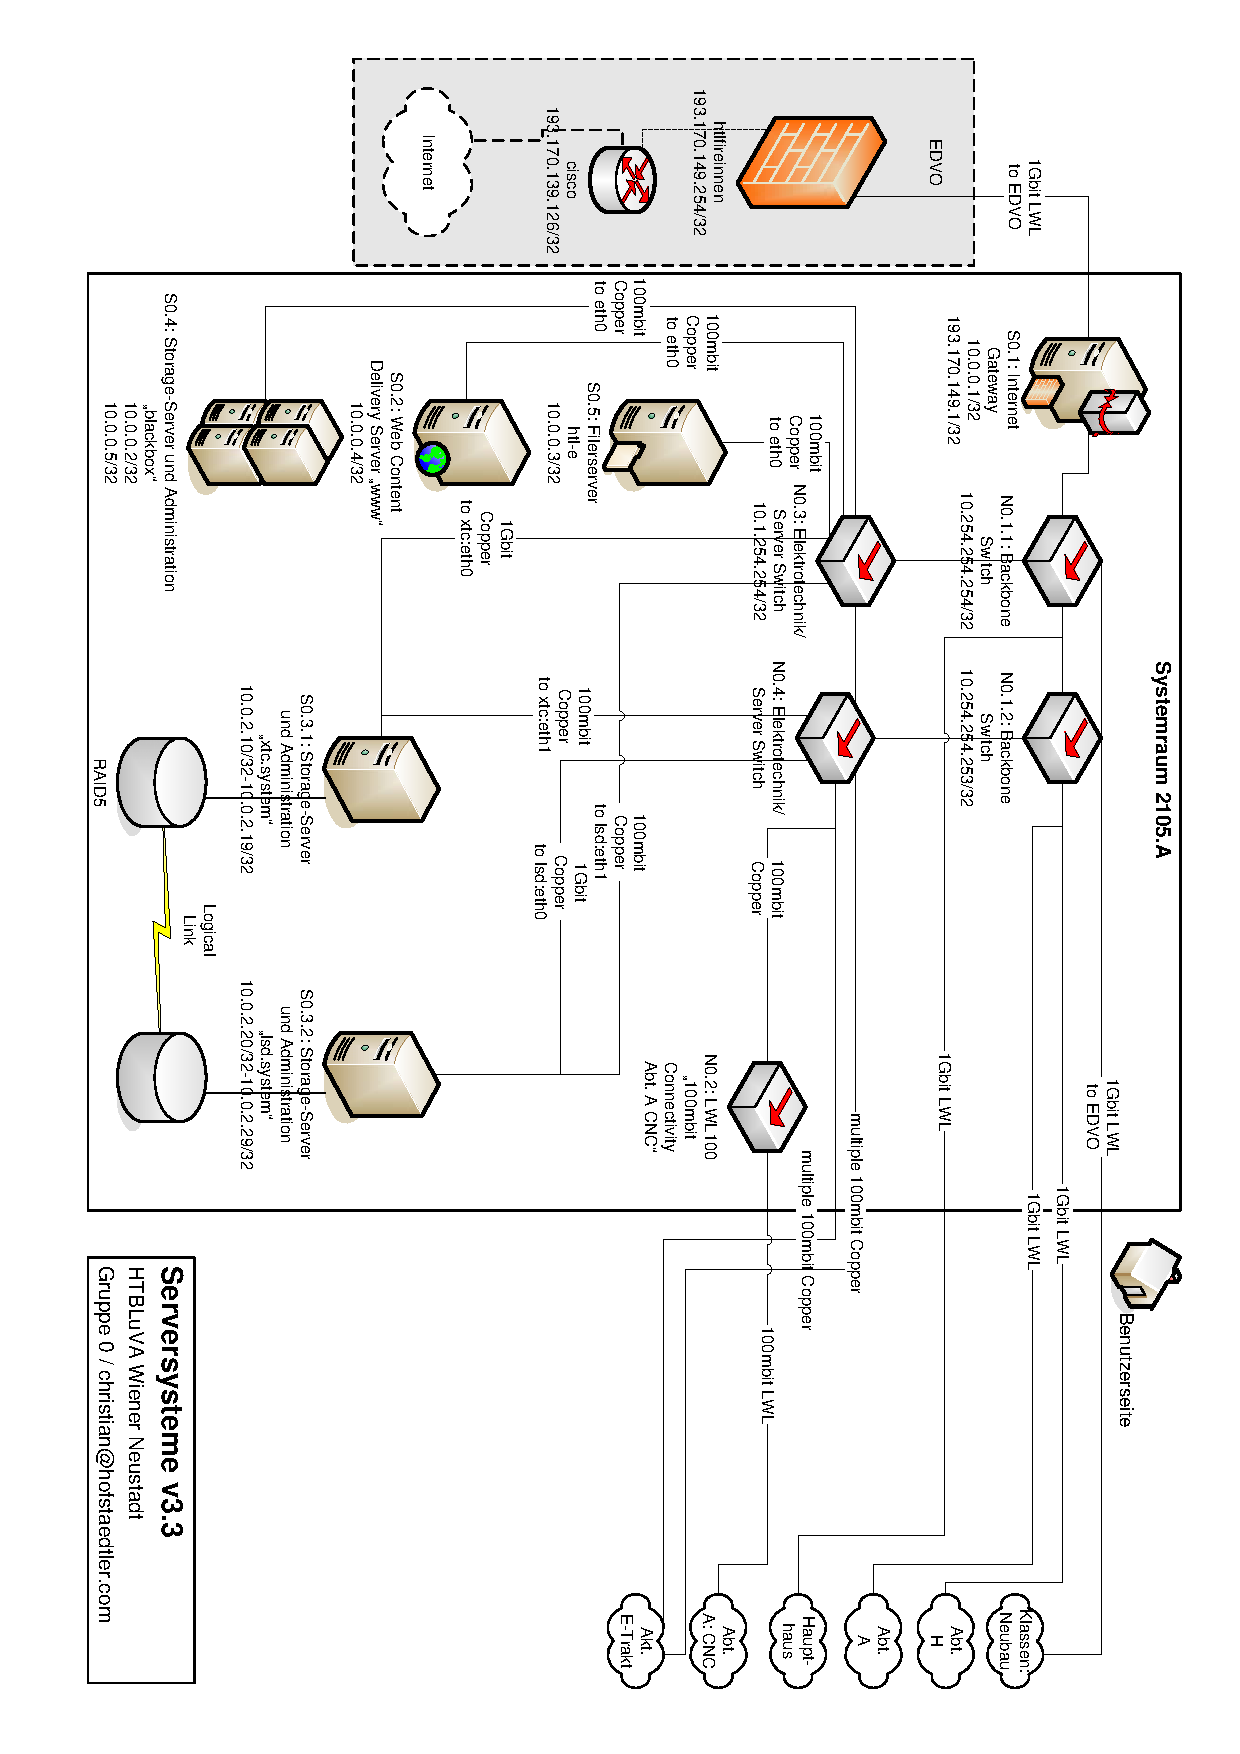
\includepdf[pages={1}]{files/htl-net-struct.pdf}
%\{htl-net-struct.pdf}{HTL Netzwerkstruktur}

\cChapter{HTL eDirectory Struktur}
\begin{landscape}
Im folgenden findet sich eine �bersicht des eDirectory Verzeichnisses. Hier mit Treename "HTL" und Basiskontext "o=htlwrn,c=at".

Der Kontext "o=System" ist nicht via LDAP sichtbar, kann daher auch nicht einfach von Applikationen ver�ndert/besch�digt werden.

\placefig{htl-nds-struct}{HTL eDirectory Struktur}

FIXME: Administration Container zeichnen.

\par

\section{Neue eDirectory Attribute}

inetStatus, loggedonHost, loggedonMac, traffic und lastActivity werden in den Benutzer-, Gruppen-, Klassen-, und Computer-Objekten verwendet. Die qbePolicy*-Attribute werden nur f�r die Computer-Policy-Objekte (qbeHostPolicy) verwendet.

\begin{lstlisting}
attributeTypes: ( 1.2.826.0.1.16224.0.0.0.10 NAME 'inetStatus' SYNTAX 1.3.6.1.4.1.1466.115.121.1.27 SINGLE-VALUE )
attributeTypes: ( 1.2.826.0.1.16224.0.0.0.11 NAME 'loggedonHost' SYNTAX 1.3.6.1.4.1.1466.115.121.1.15{64512} SINGLE-VALUE )
attributeTypes: ( 1.2.826.0.1.16224.0.0.0.12 NAME 'loggedonMac' SYNTAX 1.3.6.1.4.1.1466.115.121.1.15{128} SINGLE-VALUE )
attributeTypes: ( 1.2.826.0.1.16224.0.0.0.13 NAME 'traffic' SYNTAX 1.3.6.1.4.1.1466.115.121.1.36{64512} SINGLE-VALUE )
attributeTypes: ( 1.2.826.0.1.16224.0.0.0.14 NAME 'lastActivity' SYNTAX 1.3.6.1.4.1.1466.115.121.1.27 SINGLE-VALUE )
attributeTypes: ( 1.2.826.0.1.16224.0.0.0.15 NAME 'qbePolicyDynamicUserGroup' SYNTAX 1.3.6.1.4.1.1466.115.121.1.15{64512} )
attributeTypes: ( 1.2.826.0.1.16224.0.0.0.16 NAME 'qbePolicyDynamicUserEnabled' SYNTAX 1.3.6.1.4.1.1466.115.121.1.27 SINGLE-VALUE )
attributeTypes: ( 1.2.826.0.1.16224.0.0.0.17 NAME 'qbePolicyName' SYNTAX 1.3.6.1.4.1.1466.115.121.1.12 )
attributeTypes: ( 1.2.826.0.1.16224.0.0.0.18 NAME 'qbePolicyLoginScript' SYNTAX 1.3.6.1.4.1.1466.115.121.1.15{64512} SINGLE-VALUE )
attributeTypes: ( 1.2.826.0.1.16224.0.0.0.19 NAME 'qbePolicyHomeDrive' SYNTAX1.3.6.1.4.1.1466.115.121.1.15{64512} SINGLE-VALUE )
attributeTypes: ( 1.2.826.0.1.16224.0.0.0.20 NAME 'qbePolicyHomeDriveDir' SYNTAX 1.3.6.1.4.1.1466.115.121.1.15{64512} SINGLE-VALUE )
\end{lstlisting}

Bei einer Neuinstallation sollten die Attribute inetStatus, loggedonHost, loggedonMac, traffic und lastActivity auf qbe* umbenannt werden. Dies w�rde die Schemaverwaltung vereinfachen, zieht jedoch auch �nderungen in den PHP Skripten nach sich.


\section{Neue eDirectory Objekte}

qbeOrganizationalUnit und qbeGroup werden f�r die Klassen-/Gruppen-Verwaltung verwendet. qbeIpDevice, qbeOwnedObject und qbeHostPolicy f�r die ComputerVerwaltung.

\begin{lstlisting}
objectClasses: ( 1.2.826.0.1.16224.0.0.0.1 NAME 'qbeOrganizationalUnit' SUP organizationalUnit AUXILIARY MAY ( cn $ inetStatus ) X-NDS_NOT_CONTAINER '1' )
objectClasses: ( 1.2.826.0.1.16224.0.0.0.2 NAME 'qbeGroup' SUP groupOfNames AUXILIARY MAY inetStatus X-NDS_NOT_CONTAINER '1' )

objectClasses: ( 1.2.826.0.1.16224.0.0.0.3 NAME 'qbeIpDevice' AUXILIARY MAY ( macAddress $ ipHostNumber $ qbePolicyName ) X-NDS_NOT_CONTAINER '1' )
objectClasses: ( 1.2.826.0.1.16224.0.0.0.4 NAME 'qbeOwnedObject' AUXILIARY MAY owner X-NDS_NOT_CONTAINER '1' )
objectClasses: ( 1.2.826.0.1.16224.0.0.0.5 NAME 'qbeHostPolicy' AUXILIARY MUST qbePolicyDynamicUserEnabled MAY ( qbePolicyDynamicUserGroup $ qbePolicyHomeDrive $ qbePolicyHomeDriveDir $ qbePolicyLoginScript ) X-NDS_NOT_CONTAINER '1' )
\end{lstlisting}

\end{landscape}


\cChapter{Cluster-Installation HTL}

Der HTL-Cluster f�r den Authentication Server besteht aus zwei identischen Intel-Servern. Der Cluster-Name lautet auf qbe-auth.htlwrn.ac.at. Die Intel-Server wurden xtc.system.htlwrn.ac.at (Prim�rer Server) und lsd.system.htlwrn.ac.at (Sekund�rer Server) getauft.

Als Cluster Monitor-Software wird heartbeat eingesetzt. Die Intel-Server sind vom Modell SR2300 und mit dem Intel SE7501WV2 sowie dem Intel Raid-Controller SRCZCR ausgestattet.

Novell eDirectory wird nicht vom heartbeat verwaltet, es l�uft immer auf beiden Cluster Nodes. Alle anderen Dienste werden vom heartbeat gestartet/gestoppt.

Die Cluster-Applikationen und IP-Adressen:
\begin{description}
\item[Filesystem::/dev/nb0::/raid::ext3::noatime,usrquota,grpquota]{Das /raid (Daten-)Dateisystem}
\item[qbe-sas-daemon]{Hintergrunddienste vom Application Server}
\item[10.0.2.100]{Application Server IP}
\item[172.16.0.1/16]{Application Server IP f�r unbekannte Clients}
\item[apache::/etc/apache/httpd.conf]{Application Server Webserver}
\item[samba]{CIFS Server}
\item[mysql]{SQL Server}
\item[vsftpd]{FTP Server}
\item[nfs-kernel-server]{Network File System (NFS) Server f�r die www}
\item[dhcp3-server]{DHCP Server}
\item[10.0.2.104]{SubVersion IP}
\item[apache2]{SubVersion Server}
\end{description}


%% *eof*


% Code XRef SAS Client
\lstset{numbers=none}
%
%\cChapter{Code XRef: Qbe SAS Client Namespace Documentation}
%\hypertarget{namespaceQbe}{
\section{Qbe Namensbereichsreferenz}
\label{namespaceQbe}\index{Qbe@{Qbe}}
}




\subsection*{Klassen}
\begin{CompactItemize}
\item 
class \hyperlink{classQbe_1_1QbeClientVersion}{Qbe\-Client\-Version}
\end{CompactItemize}

%\hypertarget{namespaceQbeLoginScript}{
\section{Qbe\-Login\-Script Namensbereichsreferenz}
\label{namespaceQbeLoginScript}\index{QbeLoginScript@{QbeLoginScript}}
}




\subsection*{Klassen}
\begin{CompactItemize}
\item 
class \hyperlink{classQbeLoginScript_1_1frmLoginScript}{frm\-Login\-Script}
\item 
class \hyperlink{classQbeLoginScript_1_1InputDialog}{Input\-Dialog}
\end{CompactItemize}

%\hypertarget{namespaceQbeNDI}{
\section{Qbe\-NDI Namensbereichsreferenz}
\label{namespaceQbeNDI}\index{QbeNDI@{QbeNDI}}
}




\subsection*{Klassen}
\begin{CompactItemize}
\item 
class \hyperlink{classQbeNDI_1_1MainForm}{Main\-Form}
\item 
class \hyperlink{classQbeNDI_1_1NetConfig}{Net\-Config}
\end{CompactItemize}
\subsection*{Variablen}
\begin{CompactItemize}
\item 
char \hyperlink{namespaceQbeNDI_a0}{command\-Line} \mbox{[}514\mbox{]}
\item 
int \hyperlink{namespaceQbeNDI_a1}{prev\-Work\-State} = 0
\end{CompactItemize}


\subsection{Variablen-Dokumentation}
\hypertarget{namespaceQbeNDI_a0}{
\index{QbeNDI@{Qbe\-NDI}!commandLine@{commandLine}}
\index{commandLine@{commandLine}!QbeNDI@{Qbe\-NDI}}
\subsubsection[commandLine]{\setlength{\rightskip}{0pt plus 5cm}char \hyperlink{namespaceQbeNDI_a0}{command\-Line}\mbox{[}514\mbox{]}}}
\label{namespaceQbeNDI_a0}




Definiert in Zeile 13 der Datei Main\-Form.h.

Wird benutzt von \_\-t\-Win\-Main() und Main\-Form::tmr\-Run\_\-Tick().\hypertarget{namespaceQbeNDI_a1}{
\index{QbeNDI@{Qbe\-NDI}!prevWorkState@{prevWorkState}}
\index{prevWorkState@{prevWorkState}!QbeNDI@{Qbe\-NDI}}
\subsubsection[prevWorkState]{\setlength{\rightskip}{0pt plus 5cm}int \hyperlink{namespaceQbeNDI_a1}{prev\-Work\-State} = 0}}
\label{namespaceQbeNDI_a1}




Definiert in Zeile 14 der Datei Main\-Form.h.

Wird benutzt von Main\-Form::tmr\-Check\_\-Tick().
%\hypertarget{namespaceQbeSAS}{
\section{Qbe\-SAS Namensbereichsreferenz}
\label{namespaceQbeSAS}\index{QbeSAS@{QbeSAS}}
}




\subsection*{Klassen}
\begin{CompactItemize}
\item 
class \hyperlink{classQbeSAS_1_1ClientUI}{Client\-UI}
\begin{CompactList}\small\item\em Das gesamte Benutzerinterface des Win32 Clients. \item\end{CompactList}\item 
class \hyperlink{classQbeSAS_1_1AllCertsAreOK}{All\-Certs\-Are\-OK}
\item 
class \hyperlink{classQbeSAS_1_1HttpService}{Http\-Service}
\begin{CompactList}\small\item\em Implementiert den HTTP Dienst im Qbe\-Svc fuer alle Platformen, inklusive der Kommunikation mit dem \hyperlink{namespaceQbe}{Qbe} Authentication Server. \item\end{CompactList}\item 
class \hyperlink{classQbeSAS_1_1HttpService_1_1ServiceHttpResponse}{Http\-Service::Service\-Http\-Response}
\item 
class \hyperlink{classQbeSAS_1_1HttpService_1_1ServiceDataType}{Http\-Service::Service\-Data\-Type}
\begin{CompactList}\small\item\em Datenspeicher fuer den HTTP Service. \item\end{CompactList}\item 
class \hyperlink{classQbeSAS_1_1HttpService_1_1UriGetParameter}{Http\-Service::Uri\-Get\-Parameter}
\item 
class \hyperlink{classQbeSAS_1_1HttpService_1_1ForeignHttpResponse}{Http\-Service::Foreign\-Http\-Response}
\item 
class \hyperlink{classQbeSAS_1_1HttpService_1_1execNotificationThread}{Http\-Service::exec\-Notification\-Thread}
\item 
class \hyperlink{classQbeSAS_1_1PFC}{PFC}
\item 
class \hyperlink{classQbeSAS_1_1SysState}{Sys\-State}
\item 
class \hyperlink{classQbeSAS_1_1WinInf}{Win\-Inf}
\begin{CompactList}\small\item\em Interface fuer das Setup um den ganzen INF Stuff. \item\end{CompactList}\item 
class \hyperlink{classQbeSAS_1_1WinServiceAPI}{Win\-Service\-API}
\item 
class \hyperlink{classQbeSAS_1_1WinServiceAPI_1_1SERVICE__STATUS}{Win\-Service\-API::SERVICE\_\-STATUS}
\item 
class \hyperlink{classQbeSAS_1_1WinVersionAPI}{Win\-Version\-API}
\begin{CompactList}\small\item\em Abstraktion um das Win32 Get\-Version\-Ex() API. \item\end{CompactList}\item 
class \hyperlink{classQbeSAS_1_1WinVersionAPI_1_1OSVERSIONINFO}{Win\-Version\-API::OSVERSIONINFO}
\end{CompactItemize}

%\hypertarget{namespaceQbeService}{
\section{Qbe\-Service Namensbereichsreferenz}
\label{namespaceQbeService}\index{QbeService@{QbeService}}
}




\subsection*{Klassen}
\begin{CompactItemize}
\item 
class \hyperlink{classQbeService_1_1UnixMain}{Unix\-Main}
\begin{CompactList}\small\item\em Stellt die Umgebung fuer den XPlat-Client zur Verfuegung. \item\end{CompactList}\end{CompactItemize}

%\hypertarget{namespaceQbeStart}{
\section{Qbe\-Start Namensbereichsreferenz}
\label{namespaceQbeStart}\index{QbeStart@{QbeStart}}
}




\subsection*{Klassen}
\begin{CompactItemize}
\item 
class \hyperlink{classQbeStart_1_1Splash}{Splash}
\begin{CompactList}\small\item\em \hyperlink{classQbeStart_1_1Splash}{Splash} stellt das Start-Fenster fuer den Windows Qbe\-Server zur Verfuegung. \item\end{CompactList}\item 
class \hyperlink{classQbeStart_1_1StartX}{Start\-X}
\begin{CompactList}\small\item\em Code fuer den Client-Start, verwendet allerhand \hyperlink{namespaceQbeSAS}{Qbe\-SAS}:: Methoden und \hyperlink{classQbeStart_1_1Splash}{Qbe\-Start::Splash}. \item\end{CompactList}\end{CompactItemize}

%\hypertarget{namespaceQbeTray}{
\section{Qbe\-Tray Namensbereichsreferenz}
\label{namespaceQbeTray}\index{QbeTray@{QbeTray}}
}




\subsection*{Klassen}
\begin{CompactItemize}
\item 
class \hyperlink{classQbeTray_1_1Tray}{Tray}
\item 
class \hyperlink{classQbeTray_1_1TrayNotify}{Tray\-Notify}
\item 
struct \hyperlink{structQbeTray_1_1TrayNotify_1_1NOTIFYICONDATA}{Tray\-Notify::NOTIFYICONDATA}
\end{CompactItemize}


\cChapter{Code XRef: Qbe SAS Client Class Documentation}
%\hypertarget{struct__MSV1__0__INTERACTIVE__LOGON}{
\section{\_\-MSV1\_\-0\_\-INTERACTIVE\_\-LOGON Strukturreferenz}
\label{struct__MSV1__0__INTERACTIVE__LOGON}\index{_MSV1_0_INTERACTIVE_LOGON@{\_\-MSV1\_\-0\_\-INTERACTIVE\_\-LOGON}}
}
{\tt \#include $<$Npaux.h$>$}

\subsection*{\"{O}ffentliche Attribute}
\begin{CompactItemize}
\item 
\hyperlink{Npaux_8h_a5}{MSV1\_\-0\_\-LOGON\_\-SUBMIT\_\-TYPE} \hyperlink{struct__MSV1__0__INTERACTIVE__LOGON___MSV1__0__INTERACTIVE__LOGONo0}{Message\-Type}
\item 
\hyperlink{struct__UNICODE__STRING}{UNICODE\_\-STRING} \hyperlink{struct__MSV1__0__INTERACTIVE__LOGON___MSV1__0__INTERACTIVE__LOGONo1}{Logon\-Domain\-Name}
\item 
\hyperlink{struct__UNICODE__STRING}{UNICODE\_\-STRING} \hyperlink{struct__MSV1__0__INTERACTIVE__LOGON___MSV1__0__INTERACTIVE__LOGONo2}{User\-Name}
\item 
\hyperlink{struct__UNICODE__STRING}{UNICODE\_\-STRING} \hyperlink{struct__MSV1__0__INTERACTIVE__LOGON___MSV1__0__INTERACTIVE__LOGONo3}{Password}
\end{CompactItemize}


\subsection{Dokumentation der Datenelemente}
\hypertarget{struct__MSV1__0__INTERACTIVE__LOGON___MSV1__0__INTERACTIVE__LOGONo1}{
\index{_MSV1_0_INTERACTIVE_LOGON@{\_\-MSV1\_\-0\_\-INTERACTIVE\_\-LOGON}!LogonDomainName@{LogonDomainName}}
\index{LogonDomainName@{LogonDomainName}!_MSV1_0_INTERACTIVE_LOGON@{\_\-MSV1\_\-0\_\-INTERACTIVE\_\-LOGON}}
\subsubsection[LogonDomainName]{\setlength{\rightskip}{0pt plus 5cm}\hyperlink{struct__UNICODE__STRING}{UNICODE\_\-STRING} \hyperlink{struct__MSV1__0__INTERACTIVE__LOGON___MSV1__0__INTERACTIVE__LOGONo1}{Logon\-Domain\-Name}}}
\label{struct__MSV1__0__INTERACTIVE__LOGON___MSV1__0__INTERACTIVE__LOGONo1}




Definiert in Zeile 45 der Datei Npaux.h.\hypertarget{struct__MSV1__0__INTERACTIVE__LOGON___MSV1__0__INTERACTIVE__LOGONo0}{
\index{_MSV1_0_INTERACTIVE_LOGON@{\_\-MSV1\_\-0\_\-INTERACTIVE\_\-LOGON}!MessageType@{MessageType}}
\index{MessageType@{MessageType}!_MSV1_0_INTERACTIVE_LOGON@{\_\-MSV1\_\-0\_\-INTERACTIVE\_\-LOGON}}
\subsubsection[MessageType]{\setlength{\rightskip}{0pt plus 5cm}\hyperlink{Npaux_8h_a5}{MSV1\_\-0\_\-LOGON\_\-SUBMIT\_\-TYPE} \hyperlink{struct__MSV1__0__INTERACTIVE__LOGON___MSV1__0__INTERACTIVE__LOGONo0}{Message\-Type}}}
\label{struct__MSV1__0__INTERACTIVE__LOGON___MSV1__0__INTERACTIVE__LOGONo0}




Definiert in Zeile 44 der Datei Npaux.h.\hypertarget{struct__MSV1__0__INTERACTIVE__LOGON___MSV1__0__INTERACTIVE__LOGONo3}{
\index{_MSV1_0_INTERACTIVE_LOGON@{\_\-MSV1\_\-0\_\-INTERACTIVE\_\-LOGON}!Password@{Password}}
\index{Password@{Password}!_MSV1_0_INTERACTIVE_LOGON@{\_\-MSV1\_\-0\_\-INTERACTIVE\_\-LOGON}}
\subsubsection[Password]{\setlength{\rightskip}{0pt plus 5cm}\hyperlink{struct__UNICODE__STRING}{UNICODE\_\-STRING} \hyperlink{struct__MSV1__0__INTERACTIVE__LOGON___MSV1__0__INTERACTIVE__LOGONo3}{Password}}}
\label{struct__MSV1__0__INTERACTIVE__LOGON___MSV1__0__INTERACTIVE__LOGONo3}




Definiert in Zeile 47 der Datei Npaux.h.\hypertarget{struct__MSV1__0__INTERACTIVE__LOGON___MSV1__0__INTERACTIVE__LOGONo2}{
\index{_MSV1_0_INTERACTIVE_LOGON@{\_\-MSV1\_\-0\_\-INTERACTIVE\_\-LOGON}!UserName@{UserName}}
\index{UserName@{UserName}!_MSV1_0_INTERACTIVE_LOGON@{\_\-MSV1\_\-0\_\-INTERACTIVE\_\-LOGON}}
\subsubsection[UserName]{\setlength{\rightskip}{0pt plus 5cm}\hyperlink{struct__UNICODE__STRING}{UNICODE\_\-STRING} \hyperlink{struct__MSV1__0__INTERACTIVE__LOGON___MSV1__0__INTERACTIVE__LOGONo2}{User\-Name}}}
\label{struct__MSV1__0__INTERACTIVE__LOGON___MSV1__0__INTERACTIVE__LOGONo2}




Definiert in Zeile 46 der Datei Npaux.h.
%\hypertarget{struct__UNICODE__STRING}{
\section{\_\-UNICODE\_\-STRING Strukturreferenz}
\label{struct__UNICODE__STRING}\index{_UNICODE_STRING@{\_\-UNICODE\_\-STRING}}
}
{\tt \#include $<$Npaux.h$>$}

\subsection*{\"{O}ffentliche Attribute}
\begin{CompactItemize}
\item 
USHORT \hyperlink{struct__UNICODE__STRING___UNICODE__STRINGo0}{Length}
\item 
USHORT \hyperlink{struct__UNICODE__STRING___UNICODE__STRINGo1}{Maximum\-Length}
\item 
\hyperlink{QbeGina_8h_a8}{PWSTR} \hyperlink{struct__UNICODE__STRING___UNICODE__STRINGo2}{Buffer}
\end{CompactItemize}


\subsection{Dokumentation der Datenelemente}
\hypertarget{struct__UNICODE__STRING___UNICODE__STRINGo2}{
\index{_UNICODE_STRING@{\_\-UNICODE\_\-STRING}!Buffer@{Buffer}}
\index{Buffer@{Buffer}!_UNICODE_STRING@{\_\-UNICODE\_\-STRING}}
\subsubsection[Buffer]{\setlength{\rightskip}{0pt plus 5cm}\hyperlink{QbeGina_8h_a8}{PWSTR} \hyperlink{struct__UNICODE__STRING___UNICODE__STRINGo2}{Buffer}}}
\label{struct__UNICODE__STRING___UNICODE__STRINGo2}




Definiert in Zeile 29 der Datei Npaux.h.\hypertarget{struct__UNICODE__STRING___UNICODE__STRINGo0}{
\index{_UNICODE_STRING@{\_\-UNICODE\_\-STRING}!Length@{Length}}
\index{Length@{Length}!_UNICODE_STRING@{\_\-UNICODE\_\-STRING}}
\subsubsection[Length]{\setlength{\rightskip}{0pt plus 5cm}USHORT \hyperlink{struct__UNICODE__STRING___UNICODE__STRINGo0}{Length}}}
\label{struct__UNICODE__STRING___UNICODE__STRINGo0}




Definiert in Zeile 24 der Datei Npaux.h.\hypertarget{struct__UNICODE__STRING___UNICODE__STRINGo1}{
\index{_UNICODE_STRING@{\_\-UNICODE\_\-STRING}!MaximumLength@{MaximumLength}}
\index{MaximumLength@{MaximumLength}!_UNICODE_STRING@{\_\-UNICODE\_\-STRING}}
\subsubsection[MaximumLength]{\setlength{\rightskip}{0pt plus 5cm}USHORT \hyperlink{struct__UNICODE__STRING___UNICODE__STRINGo1}{Maximum\-Length}}}
\label{struct__UNICODE__STRING___UNICODE__STRINGo1}




Definiert in Zeile 25 der Datei Npaux.h.
\hypertarget{classQbeSAS_1_1AllCertsAreOK}{
\section{All\-Certs\-Are\-OK Klassenreferenz}
\label{classQbeSAS_1_1AllCertsAreOK}\index{QbeSAS::AllCertsAreOK@{QbeSAS::AllCertsAreOK}}
}
\subsection*{\"{O}ffentliche Methoden}
\begin{CompactItemize}
\item 
bool \hyperlink{classQbeSAS_1_1AllCertsAreOK_QbeSAS_1_1AllCertsAreOKa0}{Check\-Validation\-Result} (System.Net.Service\-Point sp, System.Security.Cryptography.X509Certificates.X509Certificate cert, System.Net.Web\-Request request, int problem)
\end{CompactItemize}


\subsection{Dokumentation der Elementfunktionen}
\hypertarget{classQbeSAS_1_1AllCertsAreOK_QbeSAS_1_1AllCertsAreOKa0}{
\index{QbeSAS::AllCertsAreOK@{Qbe\-SAS::All\-Certs\-Are\-OK}!CheckValidationResult@{CheckValidationResult}}
\index{CheckValidationResult@{CheckValidationResult}!QbeSAS::AllCertsAreOK@{Qbe\-SAS::All\-Certs\-Are\-OK}}
\subsubsection[CheckValidationResult]{\setlength{\rightskip}{0pt plus 5cm}bool Check\-Validation\-Result (System.Net.Service\-Point {\em sp}, System.Security.Cryptography.X509Certificates.X509Certificate {\em cert}, System.Net.Web\-Request {\em request}, int {\em problem})}}
\label{classQbeSAS_1_1AllCertsAreOK_QbeSAS_1_1AllCertsAreOKa0}




Definiert in Zeile 7 der Datei Http\-Service.cs.



\footnotesize\begin{verbatim}8     {
9       return true;  // as long as there is a cert, it's ok for us.
10     }
\end{verbatim}\normalsize 

\hypertarget{classQbeSAS_1_1ClientUI}{
\section{Client\-UI Klassenreferenz}
\label{classQbeSAS_1_1ClientUI}\index{QbeSAS::ClientUI@{QbeSAS::ClientUI}}
}


\subsection{Ausf\"{u}hrliche Beschreibung}
Das gesamte Benutzerinterface des Win32 Clients. 



Definiert in Zeile 6 der Datei Client\-UI.cs.\subsection*{\"{O}ffentliche Methoden}
\begin{CompactItemize}
\item 
\hyperlink{classQbeSAS_1_1ClientUI_QbeSAS_1_1ClientUIa0}{Client\-UI} (bool \hyperlink{classQbeSAS_1_1ClientUI_QbeSAS_1_1ClientUIr0}{b\-Silent})
\begin{CompactList}\small\item\em Initialisert \hyperlink{classQbeSAS_1_1ClientUI}{Client\-UI}::. Initialisert Qbe\-Directory (app\-Path) und this.b\-Silent. \item\end{CompactList}\item 
bool \hyperlink{classQbeSAS_1_1ClientUI_QbeSAS_1_1ClientUIa1}{display\-SASLogin} ()
\begin{CompactList}\small\item\em Ruft einen Browser mit dem Web-Interface Login auf. \item\end{CompactList}\item 
bool \hyperlink{classQbeSAS_1_1ClientUI_QbeSAS_1_1ClientUIa2}{display\-Client\-Login} ()
\begin{CompactList}\small\item\em Ruft die i\-Login.hta auf. \item\end{CompactList}\item 
bool \hyperlink{classQbeSAS_1_1ClientUI_QbeSAS_1_1ClientUIa3}{display\-Client\-Startup} ()
\begin{CompactList}\small\item\em Ruft die startup.hta auf. \item\end{CompactList}\item 
bool \hyperlink{classQbeSAS_1_1ClientUI_QbeSAS_1_1ClientUIa4}{import\-Settings} ()
\begin{CompactList}\small\item\em Importiert die Einstellungen (Proxy usw.) in die Registry. Dazu wird das i\-Login.reg einfach mit dem regedit importiert. \item\end{CompactList}\end{CompactItemize}
\subsection*{Private Attribute}
\begin{CompactItemize}
\item 
bool \hyperlink{classQbeSAS_1_1ClientUI_QbeSAS_1_1ClientUIr0}{b\-Silent}
\item 
String \hyperlink{classQbeSAS_1_1ClientUI_QbeSAS_1_1ClientUIr1}{app\-Path} = \char`\"{}\char`\"{}
\end{CompactItemize}


\subsection{Beschreibung der Konstruktoren und Destruktoren}
\hypertarget{classQbeSAS_1_1ClientUI_QbeSAS_1_1ClientUIa0}{
\index{QbeSAS::ClientUI@{Qbe\-SAS::Client\-UI}!ClientUI@{ClientUI}}
\index{ClientUI@{ClientUI}!QbeSAS::ClientUI@{Qbe\-SAS::Client\-UI}}
\subsubsection[ClientUI]{\setlength{\rightskip}{0pt plus 5cm}\hyperlink{classQbeSAS_1_1ClientUI}{Client\-UI} (bool {\em b\-Silent})}}
\label{classQbeSAS_1_1ClientUI_QbeSAS_1_1ClientUIa0}


Initialisert \hyperlink{classQbeSAS_1_1ClientUI}{Client\-UI}::. Initialisert Qbe\-Directory (app\-Path) und this.b\-Silent. 



Definiert in Zeile 12 der Datei Client\-UI.cs.

Benutzt Client\-UI::app\-Path.



\footnotesize\begin{verbatim}13     {
14       appPath = System.Environment.SystemDirectory;
15       if (!appPath.EndsWith("\\"))
16         appPath += "\\";
17       appPath += "Qbe\\";
18 
19       this.bSilent = bSilent;
20     }
\end{verbatim}\normalsize 


\subsection{Dokumentation der Elementfunktionen}
\hypertarget{classQbeSAS_1_1ClientUI_QbeSAS_1_1ClientUIa2}{
\index{QbeSAS::ClientUI@{Qbe\-SAS::Client\-UI}!displayClientLogin@{displayClientLogin}}
\index{displayClientLogin@{displayClientLogin}!QbeSAS::ClientUI@{Qbe\-SAS::Client\-UI}}
\subsubsection[displayClientLogin]{\setlength{\rightskip}{0pt plus 5cm}bool display\-Client\-Login ()}}
\label{classQbeSAS_1_1ClientUI_QbeSAS_1_1ClientUIa2}


Ruft die i\-Login.hta auf. 



Definiert in Zeile 40 der Datei Client\-UI.cs.

Benutzt Client\-UI::app\-Path und Client\-UI::b\-Silent.



\footnotesize\begin{verbatim}41     {
42       System.Diagnostics.ProcessStartInfo si = new System.Diagnostics.ProcessStartInfo();
43       si.WorkingDirectory = appPath;
44       si.UseShellExecute = true;
45       si.FileName = appPath + "iLogin.hta";
46       try 
47       {
48         System.Diagnostics.Process.Start(si);
49         return true;
50       } 
51       catch (Exception ex)
52       { ex=ex;
53         if (!bSilent)
54           System.Windows.Forms.MessageBox.Show("Could not find required file \"iLogin.hta\".", "Qbe SAS Client", System.Windows.Forms.MessageBoxButtons.OK, System.Windows.Forms.MessageBoxIcon.Error);
55         return false;
56       }
57     }
\end{verbatim}\normalsize 
\hypertarget{classQbeSAS_1_1ClientUI_QbeSAS_1_1ClientUIa3}{
\index{QbeSAS::ClientUI@{Qbe\-SAS::Client\-UI}!displayClientStartup@{displayClientStartup}}
\index{displayClientStartup@{displayClientStartup}!QbeSAS::ClientUI@{Qbe\-SAS::Client\-UI}}
\subsubsection[displayClientStartup]{\setlength{\rightskip}{0pt plus 5cm}bool display\-Client\-Startup ()}}
\label{classQbeSAS_1_1ClientUI_QbeSAS_1_1ClientUIa3}


Ruft die startup.hta auf. 



Definiert in Zeile 60 der Datei Client\-UI.cs.

Benutzt Client\-UI::app\-Path und Client\-UI::b\-Silent.



\footnotesize\begin{verbatim}61     {
62       System.Diagnostics.ProcessStartInfo si = new System.Diagnostics.ProcessStartInfo();
63       si.WorkingDirectory = appPath;
64       si.UseShellExecute = true;
65       si.FileName = appPath + "startup.hta";
66       try 
67       {
68         System.Diagnostics.Process.Start(si);
69         return true;
70       } 
71       catch (Exception ex)
72       { ex=ex;
73         if (!bSilent)
74           System.Windows.Forms.MessageBox.Show("Could not find required file \"startup.hta\".", "Qbe SAS Client", System.Windows.Forms.MessageBoxButtons.OK, System.Windows.Forms.MessageBoxIcon.Error);
75         return false;
76       }
77     }
\end{verbatim}\normalsize 
\hypertarget{classQbeSAS_1_1ClientUI_QbeSAS_1_1ClientUIa1}{
\index{QbeSAS::ClientUI@{Qbe\-SAS::Client\-UI}!displaySASLogin@{displaySASLogin}}
\index{displaySASLogin@{displaySASLogin}!QbeSAS::ClientUI@{Qbe\-SAS::Client\-UI}}
\subsubsection[displaySASLogin]{\setlength{\rightskip}{0pt plus 5cm}bool display\-SASLogin ()}}
\label{classQbeSAS_1_1ClientUI_QbeSAS_1_1ClientUIa1}


Ruft einen Browser mit dem Web-Interface Login auf. 



Definiert in Zeile 23 der Datei Client\-UI.cs.

Benutzt Client\-UI::b\-Silent.



\footnotesize\begin{verbatim}24     {
25       try 
26       {
27         System.Diagnostics.Process.Start( "http://qbe-auth/modules/core/checklogin.php" );
28         return true;
29       } 
30       catch (Exception ex)
31       { ex=ex;
32         if (!bSilent)
33                     System.Windows.Forms.MessageBox.Show("Could not start the default browser to view the Qbe SAS login page. Operation aborted.","Qbe SAS Client",System.Windows.Forms.MessageBoxButtons.OK,System.Windows.Forms.MessageBoxIcon.Error);
34         return false;
35       }
36 
37     }
\end{verbatim}\normalsize 
\hypertarget{classQbeSAS_1_1ClientUI_QbeSAS_1_1ClientUIa4}{
\index{QbeSAS::ClientUI@{Qbe\-SAS::Client\-UI}!importSettings@{importSettings}}
\index{importSettings@{importSettings}!QbeSAS::ClientUI@{Qbe\-SAS::Client\-UI}}
\subsubsection[importSettings]{\setlength{\rightskip}{0pt plus 5cm}bool import\-Settings ()}}
\label{classQbeSAS_1_1ClientUI_QbeSAS_1_1ClientUIa4}


Importiert die Einstellungen (Proxy usw.) in die Registry. Dazu wird das i\-Login.reg einfach mit dem regedit importiert. 



Definiert in Zeile 80 der Datei Client\-UI.cs.

Benutzt Client\-UI::app\-Path und Client\-UI::b\-Silent.



\footnotesize\begin{verbatim}81     {
82       System.Diagnostics.ProcessStartInfo si = new System.Diagnostics.ProcessStartInfo();
83       si.WorkingDirectory = appPath;
84       si.UseShellExecute = false;
85       si.FileName = "regedit.exe";
86       si.Arguments = "/s \"" + appPath + "iLogin.reg\"";
87       try 
88       {
89         System.Diagnostics.Process.Start(si);
90         return true;
91       } 
92       catch (Exception ex)
93       { ex=ex;
94         if (!bSilent)
95           System.Windows.Forms.MessageBox.Show("Could not find required file \"iLogin.reg\".", "Qbe SAS Client", System.Windows.Forms.MessageBoxButtons.OK, System.Windows.Forms.MessageBoxIcon.Error);
96         return false;
97       }
98     }
\end{verbatim}\normalsize 


\subsection{Dokumentation der Datenelemente}
\hypertarget{classQbeSAS_1_1ClientUI_QbeSAS_1_1ClientUIr1}{
\index{QbeSAS::ClientUI@{Qbe\-SAS::Client\-UI}!appPath@{appPath}}
\index{appPath@{appPath}!QbeSAS::ClientUI@{Qbe\-SAS::Client\-UI}}
\subsubsection[appPath]{\setlength{\rightskip}{0pt plus 5cm}String \hyperlink{classQbeSAS_1_1ClientUI_QbeSAS_1_1ClientUIr1}{app\-Path} = \char`\"{}\char`\"{}\hspace{0.3cm}{\tt  \mbox{[}private\mbox{]}}}}
\label{classQbeSAS_1_1ClientUI_QbeSAS_1_1ClientUIr1}




Definiert in Zeile 9 der Datei Client\-UI.cs.

Wird benutzt von Client\-UI::Client\-UI(), Client\-UI::display\-Client\-Login(), Client\-UI::display\-Client\-Startup() und Client\-UI::import\-Settings().\hypertarget{classQbeSAS_1_1ClientUI_QbeSAS_1_1ClientUIr0}{
\index{QbeSAS::ClientUI@{Qbe\-SAS::Client\-UI}!bSilent@{bSilent}}
\index{bSilent@{bSilent}!QbeSAS::ClientUI@{Qbe\-SAS::Client\-UI}}
\subsubsection[bSilent]{\setlength{\rightskip}{0pt plus 5cm}bool \hyperlink{classQbeSAS_1_1ClientUI_QbeSAS_1_1ClientUIr0}{b\-Silent}\hspace{0.3cm}{\tt  \mbox{[}private\mbox{]}}}}
\label{classQbeSAS_1_1ClientUI_QbeSAS_1_1ClientUIr0}




Definiert in Zeile 8 der Datei Client\-UI.cs.

Wird benutzt von Client\-UI::display\-Client\-Login(), Client\-UI::display\-Client\-Startup(), Client\-UI::display\-SASLogin() und Client\-UI::import\-Settings().
\hypertarget{classQbeLoginScript_1_1frmLoginScript}{
\section{frm\-Login\-Script Klassenreferenz}
\label{classQbeLoginScript_1_1frmLoginScript}\index{QbeLoginScript::frmLoginScript@{QbeLoginScript::frmLoginScript}}
}


\subsection{Ausf\"{u}hrliche Beschreibung}
Zusammenfassung f\"{u}r \hyperlink{classQbeLoginScript_1_1frmLoginScript}{frm\-Login\-Script}.  



Definiert in Zeile 13 der Datei frm\-Login\-Script.cs.\subsection*{\"{O}ffentliche Methoden}
\begin{CompactItemize}
\item 
\hyperlink{classQbeLoginScript_1_1frmLoginScript_QbeLoginScript_1_1frmLoginScripta0}{frm\-Login\-Script} ()
\item 
void \hyperlink{classQbeLoginScript_1_1frmLoginScript_QbeLoginScript_1_1frmLoginScripta1}{start\-Script} ()
\item 
void \hyperlink{classQbeLoginScript_1_1frmLoginScript_QbeLoginScript_1_1frmLoginScripta2}{Login\-Script\-Thread} ()
\item 
void \hyperlink{classQbeLoginScript_1_1frmLoginScript_QbeLoginScript_1_1frmLoginScripta3}{Read\-Std\-Out\-Thread} ()
\item 
void \hyperlink{classQbeLoginScript_1_1frmLoginScript_QbeLoginScript_1_1frmLoginScripta4}{Read\-Std\-Err\-Thread} ()
\item 
void \hyperlink{classQbeLoginScript_1_1frmLoginScript_QbeLoginScript_1_1frmLoginScripta5}{Write\-Std\-In\-Thread} ()
\end{CompactItemize}
\subsection*{Gesch\"{u}tzte Methoden}
\begin{CompactItemize}
\item 
override void \hyperlink{classQbeLoginScript_1_1frmLoginScript_QbeLoginScript_1_1frmLoginScriptb0}{Dispose} (bool disposing)
\end{CompactItemize}
\subsection*{Private Methoden}
\begin{CompactItemize}
\item 
void \hyperlink{classQbeLoginScript_1_1frmLoginScript_QbeLoginScript_1_1frmLoginScriptd0}{Add\-Login\-Script\-Output} (System.String output)
\item 
void \hyperlink{classQbeLoginScript_1_1frmLoginScript_QbeLoginScript_1_1frmLoginScriptd1}{Initialize\-Component} ()
\item 
void \hyperlink{classQbeLoginScript_1_1frmLoginScript_QbeLoginScript_1_1frmLoginScriptd2}{btn\-Close\_\-Click} (object sender, System.Event\-Args e)
\item 
void \hyperlink{classQbeLoginScript_1_1frmLoginScript_QbeLoginScript_1_1frmLoginScriptd3}{frm\-Login\-Script\_\-Load} (object sender, System.Event\-Args e)
\item 
void \hyperlink{classQbeLoginScript_1_1frmLoginScript_QbeLoginScript_1_1frmLoginScriptd4}{tmr\-Start\_\-Tick} (object sender, System.Event\-Args e)
\end{CompactItemize}
\subsection*{Private, statische Methoden}
\begin{CompactItemize}
\item 
void \hyperlink{classQbeLoginScript_1_1frmLoginScript_QbeLoginScript_1_1frmLoginScripth0}{Main} (string\mbox{[}$\,$\mbox{]} args)
\end{CompactItemize}
\subsection*{Private Attribute}
\begin{CompactItemize}
\item 
System.Windows.Forms.Button \hyperlink{classQbeLoginScript_1_1frmLoginScript_QbeLoginScript_1_1frmLoginScriptr0}{btn\-Close}
\item 
System.Windows.Forms.Text\-Box \hyperlink{classQbeLoginScript_1_1frmLoginScript_QbeLoginScript_1_1frmLoginScriptr1}{txt\-Output}
\item 
System.Windows.Forms.Picture\-Box \hyperlink{classQbeLoginScript_1_1frmLoginScript_QbeLoginScript_1_1frmLoginScriptr2}{pct\-Background}
\item 
System.String \hyperlink{classQbeLoginScript_1_1frmLoginScript_QbeLoginScript_1_1frmLoginScriptr3}{str\-Login\-Script}
\item 
System.String \hyperlink{classQbeLoginScript_1_1frmLoginScript_QbeLoginScript_1_1frmLoginScriptr4}{str\-Copied\-Login\-Script}
\item 
System.String \hyperlink{classQbeLoginScript_1_1frmLoginScript_QbeLoginScript_1_1frmLoginScriptr5}{str\-Handler}
\item 
System.String \hyperlink{classQbeLoginScript_1_1frmLoginScript_QbeLoginScript_1_1frmLoginScriptr6}{str\-Handler\-Args}
\item 
System.Boolean \hyperlink{classQbeLoginScript_1_1frmLoginScript_QbeLoginScript_1_1frmLoginScriptr7}{b\-Copy\-File}
\item 
System.Boolean \hyperlink{classQbeLoginScript_1_1frmLoginScript_QbeLoginScript_1_1frmLoginScriptr8}{b\-Auto\-Close}
\item 
System.Diagnostics.Process\-Start\-Info \hyperlink{classQbeLoginScript_1_1frmLoginScript_QbeLoginScript_1_1frmLoginScriptr9}{si\-Script}
\item 
System.Diagnostics.Process \hyperlink{classQbeLoginScript_1_1frmLoginScript_QbeLoginScript_1_1frmLoginScriptr10}{proc\-Script}
\item 
System.Threading.Thread \hyperlink{classQbeLoginScript_1_1frmLoginScript_QbeLoginScript_1_1frmLoginScriptr11}{thread\-Script}
\item 
System.Threading.Thread \hyperlink{classQbeLoginScript_1_1frmLoginScript_QbeLoginScript_1_1frmLoginScriptr12}{thread\-Write\-Std\-In}
\item 
System.Threading.Thread \hyperlink{classQbeLoginScript_1_1frmLoginScript_QbeLoginScript_1_1frmLoginScriptr13}{thread\-Read\-Std\-Out}
\item 
System.Threading.Thread \hyperlink{classQbeLoginScript_1_1frmLoginScript_QbeLoginScript_1_1frmLoginScriptr14}{thread\-Read\-Std\-Err}
\item 
System.Windows.Forms.Timer \hyperlink{classQbeLoginScript_1_1frmLoginScript_QbeLoginScript_1_1frmLoginScriptr15}{tmr\-Start}
\item 
System.Component\-Model.IContainer \hyperlink{classQbeLoginScript_1_1frmLoginScript_QbeLoginScript_1_1frmLoginScriptr16}{components}
\end{CompactItemize}


\subsection{Beschreibung der Konstruktoren und Destruktoren}
\hypertarget{classQbeLoginScript_1_1frmLoginScript_QbeLoginScript_1_1frmLoginScripta0}{
\index{QbeLoginScript::frmLoginScript@{Qbe\-Login\-Script::frm\-Login\-Script}!frmLoginScript@{frmLoginScript}}
\index{frmLoginScript@{frmLoginScript}!QbeLoginScript::frmLoginScript@{Qbe\-Login\-Script::frm\-Login\-Script}}
\subsubsection[frmLoginScript]{\setlength{\rightskip}{0pt plus 5cm}\hyperlink{classQbeLoginScript_1_1frmLoginScript}{frm\-Login\-Script} ()}}
\label{classQbeLoginScript_1_1frmLoginScript_QbeLoginScript_1_1frmLoginScripta0}




Definiert in Zeile 33 der Datei frm\-Login\-Script.cs.

Benutzt frm\-Login\-Script::Initialize\-Component().

Wird benutzt von frm\-Login\-Script::Main().



\footnotesize\begin{verbatim}34     {
35       //
36       // Erforderlich f�r die Windows Form-Designerunterst�tzung
37       //
38       InitializeComponent();
39     }
\end{verbatim}\normalsize 


\subsection{Dokumentation der Elementfunktionen}
\hypertarget{classQbeLoginScript_1_1frmLoginScript_QbeLoginScript_1_1frmLoginScriptd0}{
\index{QbeLoginScript::frmLoginScript@{Qbe\-Login\-Script::frm\-Login\-Script}!AddLoginScriptOutput@{AddLoginScriptOutput}}
\index{AddLoginScriptOutput@{AddLoginScriptOutput}!QbeLoginScript::frmLoginScript@{Qbe\-Login\-Script::frm\-Login\-Script}}
\subsubsection[AddLoginScriptOutput]{\setlength{\rightskip}{0pt plus 5cm}void Add\-Login\-Script\-Output (System.String {\em output})\hspace{0.3cm}{\tt  \mbox{[}private\mbox{]}}}}
\label{classQbeLoginScript_1_1frmLoginScript_QbeLoginScript_1_1frmLoginScriptd0}




Definiert in Zeile 129 der Datei frm\-Login\-Script.cs.

Benutzt frm\-Login\-Script::txt\-Output.

Wird benutzt von frm\-Login\-Script::Login\-Script\-Thread(), frm\-Login\-Script::Read\-Std\-Err\-Thread(), frm\-Login\-Script::Read\-Std\-Out\-Thread() und frm\-Login\-Script::start\-Script().



\footnotesize\begin{verbatim}130     {
131       this.txtOutput.Text += output + "\r\n";
132       this.txtOutput.Select(this.txtOutput.TextLength,0);
133       this.Refresh();
134       Application.DoEvents();
135     }
\end{verbatim}\normalsize 
\hypertarget{classQbeLoginScript_1_1frmLoginScript_QbeLoginScript_1_1frmLoginScriptd2}{
\index{QbeLoginScript::frmLoginScript@{Qbe\-Login\-Script::frm\-Login\-Script}!btnClose_Click@{btnClose\_\-Click}}
\index{btnClose_Click@{btnClose\_\-Click}!QbeLoginScript::frmLoginScript@{Qbe\-Login\-Script::frm\-Login\-Script}}
\subsubsection[btnClose\_\-Click]{\setlength{\rightskip}{0pt plus 5cm}void btn\-Close\_\-Click (object {\em sender}, System.Event\-Args {\em e})\hspace{0.3cm}{\tt  \mbox{[}private\mbox{]}}}}
\label{classQbeLoginScript_1_1frmLoginScript_QbeLoginScript_1_1frmLoginScriptd2}




Definiert in Zeile 314 der Datei frm\-Login\-Script.cs.

Wird benutzt von frm\-Login\-Script::Initialize\-Component().



\footnotesize\begin{verbatim}315     {
316       Application.Exit();
317     }
\end{verbatim}\normalsize 
\hypertarget{classQbeLoginScript_1_1frmLoginScript_QbeLoginScript_1_1frmLoginScriptb0}{
\index{QbeLoginScript::frmLoginScript@{Qbe\-Login\-Script::frm\-Login\-Script}!Dispose@{Dispose}}
\index{Dispose@{Dispose}!QbeLoginScript::frmLoginScript@{Qbe\-Login\-Script::frm\-Login\-Script}}
\subsubsection[Dispose]{\setlength{\rightskip}{0pt plus 5cm}override void Dispose (bool {\em disposing})\hspace{0.3cm}{\tt  \mbox{[}protected\mbox{]}}}}
\label{classQbeLoginScript_1_1frmLoginScript_QbeLoginScript_1_1frmLoginScriptb0}


Die verwendeten Ressourcen bereinigen.  

Definiert in Zeile 183 der Datei frm\-Login\-Script.cs.

Benutzt frm\-Login\-Script::components.



\footnotesize\begin{verbatim}184     {
185       if( disposing )
186       {
187         if (components != null) 
188         {
189           components.Dispose();
190         }
191       }
192       base.Dispose( disposing );
193     }
\end{verbatim}\normalsize 
\hypertarget{classQbeLoginScript_1_1frmLoginScript_QbeLoginScript_1_1frmLoginScriptd3}{
\index{QbeLoginScript::frmLoginScript@{Qbe\-Login\-Script::frm\-Login\-Script}!frmLoginScript_Load@{frmLoginScript\_\-Load}}
\index{frmLoginScript_Load@{frmLoginScript\_\-Load}!QbeLoginScript::frmLoginScript@{Qbe\-Login\-Script::frm\-Login\-Script}}
\subsubsection[frmLoginScript\_\-Load]{\setlength{\rightskip}{0pt plus 5cm}void frm\-Login\-Script\_\-Load (object {\em sender}, System.Event\-Args {\em e})\hspace{0.3cm}{\tt  \mbox{[}private\mbox{]}}}}
\label{classQbeLoginScript_1_1frmLoginScript_QbeLoginScript_1_1frmLoginScriptd3}




Definiert in Zeile 319 der Datei frm\-Login\-Script.cs.

Benutzt frm\-Login\-Script::tmr\-Start.

Wird benutzt von frm\-Login\-Script::Initialize\-Component().



\footnotesize\begin{verbatim}320     {
321       this.Show();
322       this.WindowState = System.Windows.Forms.FormWindowState.Normal;
323       Application.DoEvents();
324       tmrStart.Enabled = true;
325     }
\end{verbatim}\normalsize 
\hypertarget{classQbeLoginScript_1_1frmLoginScript_QbeLoginScript_1_1frmLoginScriptd1}{
\index{QbeLoginScript::frmLoginScript@{Qbe\-Login\-Script::frm\-Login\-Script}!InitializeComponent@{InitializeComponent}}
\index{InitializeComponent@{InitializeComponent}!QbeLoginScript::frmLoginScript@{Qbe\-Login\-Script::frm\-Login\-Script}}
\subsubsection[InitializeComponent]{\setlength{\rightskip}{0pt plus 5cm}void Initialize\-Component ()\hspace{0.3cm}{\tt  \mbox{[}private\mbox{]}}}}
\label{classQbeLoginScript_1_1frmLoginScript_QbeLoginScript_1_1frmLoginScriptd1}


Erforderliche Methode f\"{u}r die Designerunterst\"{u}tzung. Der Inhalt der Methode darf nicht mit dem Code-Editor ge\"{a}ndert werden.  

Definiert in Zeile 200 der Datei frm\-Login\-Script.cs.

Benutzt frm\-Login\-Script::btn\-Close, frm\-Login\-Script::btn\-Close\_\-Click(), frm\-Login\-Script::components, frm\-Login\-Script::frm\-Login\-Script\_\-Load(), frm\-Login\-Script::pct\-Background, frm\-Login\-Script::tmr\-Start\_\-Tick() und frm\-Login\-Script::txt\-Output.

Wird benutzt von frm\-Login\-Script::frm\-Login\-Script().



\footnotesize\begin{verbatim}201     {
202       this.components = new System.ComponentModel.Container();
203       System.Resources.ResourceManager resources = new System.Resources.ResourceManager("frmLoginScript",System.Reflection.Assembly.GetExecutingAssembly());
204       this.btnClose = new System.Windows.Forms.Button();
205       this.txtOutput = new System.Windows.Forms.TextBox();
206       this.pctBackground = new System.Windows.Forms.PictureBox();
207       this.tmrStart = new System.Windows.Forms.Timer(this.components);
208       this.SuspendLayout();
209       // 
210       // btnClose
211       // 
212       this.btnClose.Anchor = ((System.Windows.Forms.AnchorStyles)(((System.Windows.Forms.AnchorStyles.Bottom | System.Windows.Forms.AnchorStyles.Left) 
213         | System.Windows.Forms.AnchorStyles.Right)));
214       this.btnClose.BackColor = System.Drawing.SystemColors.Control;
215       this.btnClose.DialogResult = System.Windows.Forms.DialogResult.Cancel;
216       this.btnClose.Enabled = false;
217       this.btnClose.Location = new System.Drawing.Point(200, 384);
218       this.btnClose.Name = "btnClose";
219       this.btnClose.Size = new System.Drawing.Size(80, 24);
220       this.btnClose.TabIndex = 0;
221       this.btnClose.Text = "Close";
222       this.btnClose.Click += new System.EventHandler(this.btnClose_Click);
223       // 
224       // txtOutput
225       // 
226       this.txtOutput.Anchor = ((System.Windows.Forms.AnchorStyles)((((System.Windows.Forms.AnchorStyles.Top | System.Windows.Forms.AnchorStyles.Bottom) 
227         | System.Windows.Forms.AnchorStyles.Left) 
228         | System.Windows.Forms.AnchorStyles.Right)));
229       this.txtOutput.AutoSize = false;
230       this.txtOutput.BackColor = System.Drawing.Color.FromArgb(((System.Byte)(51)), ((System.Byte)(102)), ((System.Byte)(153)));
231       this.txtOutput.BorderStyle = System.Windows.Forms.BorderStyle.None;
232       this.txtOutput.ForeColor = System.Drawing.Color.White;
233       this.txtOutput.Location = new System.Drawing.Point(8, 88);
234       this.txtOutput.Multiline = true;
235       this.txtOutput.Name = "txtOutput";
236       this.txtOutput.ReadOnly = true;
237       this.txtOutput.ScrollBars = System.Windows.Forms.ScrollBars.Both;
238       this.txtOutput.Size = new System.Drawing.Size(464, 288);
239       this.txtOutput.TabIndex = 1;
240       this.txtOutput.Text = "";
241       // 
242       // pctBackground
243       // 
244       this.pctBackground.BackColor = System.Drawing.Color.Transparent;
245       this.pctBackground.Image = ((System.Drawing.Image)(resources.GetObject("pctBackground.Image")));
246       this.pctBackground.Location = new System.Drawing.Point(0, 0);
247       this.pctBackground.Name = "pctBackground";
248       this.pctBackground.Size = new System.Drawing.Size(400, 200);
249       this.pctBackground.SizeMode = System.Windows.Forms.PictureBoxSizeMode.AutoSize;
250       this.pctBackground.TabIndex = 2;
251       this.pctBackground.TabStop = false;
252       // 
253       // tmrStart
254       // 
255       this.tmrStart.Tick += new System.EventHandler(this.tmrStart_Tick);
256       // 
257       // frmLoginScript
258       // 
259       this.AcceptButton = this.btnClose;
260       this.AutoScaleBaseSize = new System.Drawing.Size(5, 13);
261       this.BackColor = System.Drawing.Color.FromArgb(((System.Byte)(51)), ((System.Byte)(102)), ((System.Byte)(153)));
262       this.CancelButton = this.btnClose;
263       this.ClientSize = new System.Drawing.Size(480, 414);
264       this.ControlBox = false;
265       this.Controls.Add(this.txtOutput);
266       this.Controls.Add(this.btnClose);
267       this.Controls.Add(this.pctBackground);
268       this.MaximizeBox = false;
269       this.MinimizeBox = false;
270       this.Name = "frmLoginScript";
271       this.StartPosition = System.Windows.Forms.FormStartPosition.CenterScreen;
272       this.Text = "Qbe Login Script";
273       this.Load += new System.EventHandler(this.frmLoginScript_Load);
274       this.ResumeLayout(false);
275 
276     }
\end{verbatim}\normalsize 
\hypertarget{classQbeLoginScript_1_1frmLoginScript_QbeLoginScript_1_1frmLoginScripta2}{
\index{QbeLoginScript::frmLoginScript@{Qbe\-Login\-Script::frm\-Login\-Script}!LoginScriptThread@{LoginScriptThread}}
\index{LoginScriptThread@{LoginScriptThread}!QbeLoginScript::frmLoginScript@{Qbe\-Login\-Script::frm\-Login\-Script}}
\subsubsection[LoginScriptThread]{\setlength{\rightskip}{0pt plus 5cm}void Login\-Script\-Thread ()}}
\label{classQbeLoginScript_1_1frmLoginScript_QbeLoginScript_1_1frmLoginScripta2}




Definiert in Zeile 95 der Datei frm\-Login\-Script.cs.

Benutzt frm\-Login\-Script::Add\-Login\-Script\-Output(), frm\-Login\-Script::btn\-Close, frm\-Login\-Script::proc\-Script, frm\-Login\-Script::str\-Copied\-Login\-Script, frm\-Login\-Script::thread\-Read\-Std\-Err, frm\-Login\-Script::thread\-Read\-Std\-Out und frm\-Login\-Script::thread\-Write\-Std\-In.

Wird benutzt von frm\-Login\-Script::start\-Script().



\footnotesize\begin{verbatim}96     {
97       this.procScript.WaitForExit();
98       btnClose.Enabled = true;
99       Application.DoEvents();
100 
101       try 
102       {
103         threadWriteStdIn.Abort();
104         threadReadStdOut.Abort();
105         threadReadStdErr.Abort();
106 
107         if (this.bCopyFile)
108         { // delete the file we created.
109           try {System.IO.File.Delete(this.strCopiedLoginScript);}  
110           catch (Exception ex) {ex=ex; MessageBox.Show("ex handler"); }
111         }
112 
113         AddLoginScriptOutput("");
114         AddLoginScriptOutput("Qbe Login Script returned Exit Code " + this.procScript.ExitCode.ToString());
115 
116 
117         if ((this.procScript.ExitCode == 0) && (this.bAutoClose))
118         {
119           this.Close();
120         }
121       }
122       catch (Exception ex)
123       {
124         ex=ex;
125       }
126 
127     }
\end{verbatim}\normalsize 
\hypertarget{classQbeLoginScript_1_1frmLoginScript_QbeLoginScript_1_1frmLoginScripth0}{
\index{QbeLoginScript::frmLoginScript@{Qbe\-Login\-Script::frm\-Login\-Script}!Main@{Main}}
\index{Main@{Main}!QbeLoginScript::frmLoginScript@{Qbe\-Login\-Script::frm\-Login\-Script}}
\subsubsection[Main]{\setlength{\rightskip}{0pt plus 5cm}void Main (string\mbox{[}$\,$\mbox{]} {\em args})\hspace{0.3cm}{\tt  \mbox{[}static, private\mbox{]}}}}
\label{classQbeLoginScript_1_1frmLoginScript_QbeLoginScript_1_1frmLoginScripth0}


Der Haupteinstiegspunkt f\"{u}r die Anwendung.  

Definiert in Zeile 283 der Datei frm\-Login\-Script.cs.

Benutzt frm\-Login\-Script::b\-Auto\-Close, frm\-Login\-Script::b\-Copy\-File, frm\-Login\-Script::frm\-Login\-Script(), frm\-Login\-Script::str\-Handler, frm\-Login\-Script::str\-Handler\-Args und frm\-Login\-Script::str\-Login\-Script.



\footnotesize\begin{verbatim}284     {
285       if (args.Length < 4)
286       {
287         MessageBox.Show("Usage: QbeLoginScript.exe HandlerPath HandlerArgs LoginScriptFile [CopyLoginScript = FALSE] [AutoCloseWindow = TRUE]","Qbe SAS Client");
288         return;
289       }
290       
291       try 
292       {
293         frmLoginScript frm;
294         frm = new frmLoginScript();
295         frm.strHandler = args[0];
296         frm.strHandlerArgs = args[1];
297         frm.strLoginScript = args[2];
298         if (args.Length > 3)
299           frm.bCopyFile = System.Boolean.Parse(args[3]);
300         else
301           frm.bCopyFile = false;
302         if (args.Length > 4)
303           frm.bAutoClose = System.Boolean.Parse(args[4]);
304         else
305           frm.bAutoClose = true;
306         Application.Run(frm);
307       } 
308       catch (Exception ex)
309       {
310         MessageBox.Show("Error: "+ ex.Message + "\r\n" +ex.StackTrace,"Qbe SAS Login",System.Windows.Forms.MessageBoxButtons.OK,System.Windows.Forms.MessageBoxIcon.Error);
311       }
312     }
\end{verbatim}\normalsize 
\hypertarget{classQbeLoginScript_1_1frmLoginScript_QbeLoginScript_1_1frmLoginScripta4}{
\index{QbeLoginScript::frmLoginScript@{Qbe\-Login\-Script::frm\-Login\-Script}!ReadStdErrThread@{ReadStdErrThread}}
\index{ReadStdErrThread@{ReadStdErrThread}!QbeLoginScript::frmLoginScript@{Qbe\-Login\-Script::frm\-Login\-Script}}
\subsubsection[ReadStdErrThread]{\setlength{\rightskip}{0pt plus 5cm}void Read\-Std\-Err\-Thread ()}}
\label{classQbeLoginScript_1_1frmLoginScript_QbeLoginScript_1_1frmLoginScripta4}




Definiert in Zeile 145 der Datei frm\-Login\-Script.cs.

Benutzt frm\-Login\-Script::Add\-Login\-Script\-Output() und frm\-Login\-Script::proc\-Script.

Wird benutzt von frm\-Login\-Script::start\-Script().



\footnotesize\begin{verbatim}146     {
147       string output;
148       while ((output = procScript.StandardError.ReadLine()) != null)
149       {
150         AddLoginScriptOutput(output);
151       }
152     }
\end{verbatim}\normalsize 
\hypertarget{classQbeLoginScript_1_1frmLoginScript_QbeLoginScript_1_1frmLoginScripta3}{
\index{QbeLoginScript::frmLoginScript@{Qbe\-Login\-Script::frm\-Login\-Script}!ReadStdOutThread@{ReadStdOutThread}}
\index{ReadStdOutThread@{ReadStdOutThread}!QbeLoginScript::frmLoginScript@{Qbe\-Login\-Script::frm\-Login\-Script}}
\subsubsection[ReadStdOutThread]{\setlength{\rightskip}{0pt plus 5cm}void Read\-Std\-Out\-Thread ()}}
\label{classQbeLoginScript_1_1frmLoginScript_QbeLoginScript_1_1frmLoginScripta3}




Definiert in Zeile 137 der Datei frm\-Login\-Script.cs.

Benutzt frm\-Login\-Script::Add\-Login\-Script\-Output() und frm\-Login\-Script::proc\-Script.

Wird benutzt von frm\-Login\-Script::start\-Script().



\footnotesize\begin{verbatim}138     {     
139       string output;
140       while ((output = procScript.StandardOutput.ReadLine()) != null)
141       {
142         AddLoginScriptOutput(output);
143       }
144     }
\end{verbatim}\normalsize 
\hypertarget{classQbeLoginScript_1_1frmLoginScript_QbeLoginScript_1_1frmLoginScripta1}{
\index{QbeLoginScript::frmLoginScript@{Qbe\-Login\-Script::frm\-Login\-Script}!startScript@{startScript}}
\index{startScript@{startScript}!QbeLoginScript::frmLoginScript@{Qbe\-Login\-Script::frm\-Login\-Script}}
\subsubsection[startScript]{\setlength{\rightskip}{0pt plus 5cm}void start\-Script ()}}
\label{classQbeLoginScript_1_1frmLoginScript_QbeLoginScript_1_1frmLoginScripta1}




Definiert in Zeile 41 der Datei frm\-Login\-Script.cs.

Benutzt frm\-Login\-Script::Add\-Login\-Script\-Output(), frm\-Login\-Script::b\-Auto\-Close, frm\-Login\-Script::b\-Copy\-File, frm\-Login\-Script::Login\-Script\-Thread(), frm\-Login\-Script::proc\-Script, frm\-Login\-Script::Read\-Std\-Err\-Thread(), frm\-Login\-Script::Read\-Std\-Out\-Thread(), frm\-Login\-Script::si\-Script, frm\-Login\-Script::str\-Handler, frm\-Login\-Script::str\-Handler\-Args, frm\-Login\-Script::str\-Login\-Script, frm\-Login\-Script::thread\-Read\-Std\-Err, frm\-Login\-Script::thread\-Read\-Std\-Out, frm\-Login\-Script::thread\-Script, frm\-Login\-Script::thread\-Write\-Std\-In und frm\-Login\-Script::Write\-Std\-In\-Thread().



\footnotesize\begin{verbatim}42     {
43       System.String strScript;
44 
45       try 
46       {
47 
48         if (this.bCopyFile)
49         {
50           System.String newFileName = System.IO.Path.GetTempPath() + "\\" + System.IO.Path.GetFileName(this.strLoginScript);
51           try {System.IO.File.Delete(newFileName);}  
52           catch (Exception ex) {ex=ex; MessageBox.Show("ex handler"); }
53           System.IO.File.Copy(this.strLoginScript,newFileName);
54           strScript = newFileName;
55           this.strCopiedLoginScript = newFileName;
56         } 
57         else 
58         {
59           strScript = this.strLoginScript;
60         }
61 
62         AddLoginScriptOutput("Qbe Login Script: " + strScript);
63         AddLoginScriptOutput("AutoClose: " + this.bAutoClose);
64         AddLoginScriptOutput("CopyScript: " + this.bCopyFile);
65 
66         siScript = new System.Diagnostics.ProcessStartInfo(strHandler,strHandlerArgs);
67         siScript.CreateNoWindow = true;
68         siScript.RedirectStandardError = true;
69         siScript.RedirectStandardOutput = true;
70         siScript.RedirectStandardInput = true;
71         siScript.WorkingDirectory = System.IO.Path.GetPathRoot(strScript);
72         siScript.UseShellExecute = false;
73 
74         procScript = new System.Diagnostics.Process();
75         procScript.StartInfo = siScript;
76 
77         threadScript = new System.Threading.Thread(new System.Threading.ThreadStart(LoginScriptThread));
78         threadWriteStdIn = new System.Threading.Thread(new System.Threading.ThreadStart(WriteStdInThread));
79         threadReadStdOut = new System.Threading.Thread(new System.Threading.ThreadStart(ReadStdOutThread));
80         threadReadStdErr = new System.Threading.Thread(new System.Threading.ThreadStart(ReadStdErrThread));
81 
82         procScript.Start();
83         threadScript.Start();
84         threadWriteStdIn.Start();
85         threadReadStdOut.Start();
86         threadReadStdErr.Start();
87       } 
88       catch (Exception ex)
89       {
90         MessageBox.Show("Error: "+ ex.Message + "\r\n" +ex.StackTrace,"Qbe SAS Login",System.Windows.Forms.MessageBoxButtons.OK,System.Windows.Forms.MessageBoxIcon.Error);
91       }
92     }
\end{verbatim}\normalsize 
\hypertarget{classQbeLoginScript_1_1frmLoginScript_QbeLoginScript_1_1frmLoginScriptd4}{
\index{QbeLoginScript::frmLoginScript@{Qbe\-Login\-Script::frm\-Login\-Script}!tmrStart_Tick@{tmrStart\_\-Tick}}
\index{tmrStart_Tick@{tmrStart\_\-Tick}!QbeLoginScript::frmLoginScript@{Qbe\-Login\-Script::frm\-Login\-Script}}
\subsubsection[tmrStart\_\-Tick]{\setlength{\rightskip}{0pt plus 5cm}void tmr\-Start\_\-Tick (object {\em sender}, System.Event\-Args {\em e})\hspace{0.3cm}{\tt  \mbox{[}private\mbox{]}}}}
\label{classQbeLoginScript_1_1frmLoginScript_QbeLoginScript_1_1frmLoginScriptd4}




Definiert in Zeile 327 der Datei frm\-Login\-Script.cs.

Wird benutzt von frm\-Login\-Script::Initialize\-Component().



\footnotesize\begin{verbatim}328     {
329       this.tmrStart.Enabled = false;
330       this.startScript();
331     }
\end{verbatim}\normalsize 
\hypertarget{classQbeLoginScript_1_1frmLoginScript_QbeLoginScript_1_1frmLoginScripta5}{
\index{QbeLoginScript::frmLoginScript@{Qbe\-Login\-Script::frm\-Login\-Script}!WriteStdInThread@{WriteStdInThread}}
\index{WriteStdInThread@{WriteStdInThread}!QbeLoginScript::frmLoginScript@{Qbe\-Login\-Script::frm\-Login\-Script}}
\subsubsection[WriteStdInThread]{\setlength{\rightskip}{0pt plus 5cm}void Write\-Std\-In\-Thread ()}}
\label{classQbeLoginScript_1_1frmLoginScript_QbeLoginScript_1_1frmLoginScripta5}




Definiert in Zeile 153 der Datei frm\-Login\-Script.cs.

Wird benutzt von frm\-Login\-Script::start\-Script().



\footnotesize\begin{verbatim}154     {
155     /*  while (!procScript.HasExited)
156       {
157         try 
158         {
159           procScript.WaitForInputIdle();
160         } 
161         catch (Exception ex)
162         {
163           try 
164           {
165             ex=ex;
166             InputDialog dlg = new InputDialog();
167             dlg.ShowDialog(this);
168             procScript.StandardInput.WriteLine(dlg.strAnswer); 
169 
170             this.Refresh();
171             Application.DoEvents();
172             System.Threading.Thread.Sleep(100);
173           } 
174           catch (Exception ex2) { ex2=ex2; }
175         }
176       } 
177       */
178     }
\end{verbatim}\normalsize 


\subsection{Dokumentation der Datenelemente}
\hypertarget{classQbeLoginScript_1_1frmLoginScript_QbeLoginScript_1_1frmLoginScriptr8}{
\index{QbeLoginScript::frmLoginScript@{Qbe\-Login\-Script::frm\-Login\-Script}!bAutoClose@{bAutoClose}}
\index{bAutoClose@{bAutoClose}!QbeLoginScript::frmLoginScript@{Qbe\-Login\-Script::frm\-Login\-Script}}
\subsubsection[bAutoClose]{\setlength{\rightskip}{0pt plus 5cm}System.Boolean \hyperlink{classQbeLoginScript_1_1frmLoginScript_QbeLoginScript_1_1frmLoginScriptr8}{b\-Auto\-Close}\hspace{0.3cm}{\tt  \mbox{[}private\mbox{]}}}}
\label{classQbeLoginScript_1_1frmLoginScript_QbeLoginScript_1_1frmLoginScriptr8}




Definiert in Zeile 23 der Datei frm\-Login\-Script.cs.

Wird benutzt von frm\-Login\-Script::Main() und frm\-Login\-Script::start\-Script().\hypertarget{classQbeLoginScript_1_1frmLoginScript_QbeLoginScript_1_1frmLoginScriptr7}{
\index{QbeLoginScript::frmLoginScript@{Qbe\-Login\-Script::frm\-Login\-Script}!bCopyFile@{bCopyFile}}
\index{bCopyFile@{bCopyFile}!QbeLoginScript::frmLoginScript@{Qbe\-Login\-Script::frm\-Login\-Script}}
\subsubsection[bCopyFile]{\setlength{\rightskip}{0pt plus 5cm}System.Boolean \hyperlink{classQbeLoginScript_1_1frmLoginScript_QbeLoginScript_1_1frmLoginScriptr7}{b\-Copy\-File}\hspace{0.3cm}{\tt  \mbox{[}private\mbox{]}}}}
\label{classQbeLoginScript_1_1frmLoginScript_QbeLoginScript_1_1frmLoginScriptr7}




Definiert in Zeile 22 der Datei frm\-Login\-Script.cs.

Wird benutzt von frm\-Login\-Script::Main() und frm\-Login\-Script::start\-Script().\hypertarget{classQbeLoginScript_1_1frmLoginScript_QbeLoginScript_1_1frmLoginScriptr0}{
\index{QbeLoginScript::frmLoginScript@{Qbe\-Login\-Script::frm\-Login\-Script}!btnClose@{btnClose}}
\index{btnClose@{btnClose}!QbeLoginScript::frmLoginScript@{Qbe\-Login\-Script::frm\-Login\-Script}}
\subsubsection[btnClose]{\setlength{\rightskip}{0pt plus 5cm}System.Windows.Forms.Button \hyperlink{classQbeLoginScript_1_1frmLoginScript_QbeLoginScript_1_1frmLoginScriptr0}{btn\-Close}\hspace{0.3cm}{\tt  \mbox{[}private\mbox{]}}}}
\label{classQbeLoginScript_1_1frmLoginScript_QbeLoginScript_1_1frmLoginScriptr0}




Definiert in Zeile 15 der Datei frm\-Login\-Script.cs.

Wird benutzt von frm\-Login\-Script::Initialize\-Component() und frm\-Login\-Script::Login\-Script\-Thread().\hypertarget{classQbeLoginScript_1_1frmLoginScript_QbeLoginScript_1_1frmLoginScriptr16}{
\index{QbeLoginScript::frmLoginScript@{Qbe\-Login\-Script::frm\-Login\-Script}!components@{components}}
\index{components@{components}!QbeLoginScript::frmLoginScript@{Qbe\-Login\-Script::frm\-Login\-Script}}
\subsubsection[components]{\setlength{\rightskip}{0pt plus 5cm}System.Component\-Model.IContainer \hyperlink{classQbeLoginScript_1_1frmLoginScript_QbeLoginScript_1_1frmLoginScriptr16}{components}\hspace{0.3cm}{\tt  \mbox{[}private\mbox{]}}}}
\label{classQbeLoginScript_1_1frmLoginScript_QbeLoginScript_1_1frmLoginScriptr16}




Definiert in Zeile 31 der Datei frm\-Login\-Script.cs.

Wird benutzt von frm\-Login\-Script::Dispose() und frm\-Login\-Script::Initialize\-Component().\hypertarget{classQbeLoginScript_1_1frmLoginScript_QbeLoginScript_1_1frmLoginScriptr2}{
\index{QbeLoginScript::frmLoginScript@{Qbe\-Login\-Script::frm\-Login\-Script}!pctBackground@{pctBackground}}
\index{pctBackground@{pctBackground}!QbeLoginScript::frmLoginScript@{Qbe\-Login\-Script::frm\-Login\-Script}}
\subsubsection[pctBackground]{\setlength{\rightskip}{0pt plus 5cm}System.Windows.Forms.Picture\-Box \hyperlink{classQbeLoginScript_1_1frmLoginScript_QbeLoginScript_1_1frmLoginScriptr2}{pct\-Background}\hspace{0.3cm}{\tt  \mbox{[}private\mbox{]}}}}
\label{classQbeLoginScript_1_1frmLoginScript_QbeLoginScript_1_1frmLoginScriptr2}




Definiert in Zeile 17 der Datei frm\-Login\-Script.cs.

Wird benutzt von frm\-Login\-Script::Initialize\-Component().\hypertarget{classQbeLoginScript_1_1frmLoginScript_QbeLoginScript_1_1frmLoginScriptr10}{
\index{QbeLoginScript::frmLoginScript@{Qbe\-Login\-Script::frm\-Login\-Script}!procScript@{procScript}}
\index{procScript@{procScript}!QbeLoginScript::frmLoginScript@{Qbe\-Login\-Script::frm\-Login\-Script}}
\subsubsection[procScript]{\setlength{\rightskip}{0pt plus 5cm}System.Diagnostics.Process \hyperlink{classQbeLoginScript_1_1frmLoginScript_QbeLoginScript_1_1frmLoginScriptr10}{proc\-Script}\hspace{0.3cm}{\tt  \mbox{[}private\mbox{]}}}}
\label{classQbeLoginScript_1_1frmLoginScript_QbeLoginScript_1_1frmLoginScriptr10}




Definiert in Zeile 25 der Datei frm\-Login\-Script.cs.

Wird benutzt von frm\-Login\-Script::Login\-Script\-Thread(), frm\-Login\-Script::Read\-Std\-Err\-Thread(), frm\-Login\-Script::Read\-Std\-Out\-Thread() und frm\-Login\-Script::start\-Script().\hypertarget{classQbeLoginScript_1_1frmLoginScript_QbeLoginScript_1_1frmLoginScriptr9}{
\index{QbeLoginScript::frmLoginScript@{Qbe\-Login\-Script::frm\-Login\-Script}!siScript@{siScript}}
\index{siScript@{siScript}!QbeLoginScript::frmLoginScript@{Qbe\-Login\-Script::frm\-Login\-Script}}
\subsubsection[siScript]{\setlength{\rightskip}{0pt plus 5cm}System.Diagnostics.Process\-Start\-Info \hyperlink{classQbeLoginScript_1_1frmLoginScript_QbeLoginScript_1_1frmLoginScriptr9}{si\-Script}\hspace{0.3cm}{\tt  \mbox{[}private\mbox{]}}}}
\label{classQbeLoginScript_1_1frmLoginScript_QbeLoginScript_1_1frmLoginScriptr9}




Definiert in Zeile 24 der Datei frm\-Login\-Script.cs.

Wird benutzt von frm\-Login\-Script::start\-Script().\hypertarget{classQbeLoginScript_1_1frmLoginScript_QbeLoginScript_1_1frmLoginScriptr4}{
\index{QbeLoginScript::frmLoginScript@{Qbe\-Login\-Script::frm\-Login\-Script}!strCopiedLoginScript@{strCopiedLoginScript}}
\index{strCopiedLoginScript@{strCopiedLoginScript}!QbeLoginScript::frmLoginScript@{Qbe\-Login\-Script::frm\-Login\-Script}}
\subsubsection[strCopiedLoginScript]{\setlength{\rightskip}{0pt plus 5cm}System.String \hyperlink{classQbeLoginScript_1_1frmLoginScript_QbeLoginScript_1_1frmLoginScriptr4}{str\-Copied\-Login\-Script}\hspace{0.3cm}{\tt  \mbox{[}private\mbox{]}}}}
\label{classQbeLoginScript_1_1frmLoginScript_QbeLoginScript_1_1frmLoginScriptr4}




Definiert in Zeile 19 der Datei frm\-Login\-Script.cs.

Wird benutzt von frm\-Login\-Script::Login\-Script\-Thread().\hypertarget{classQbeLoginScript_1_1frmLoginScript_QbeLoginScript_1_1frmLoginScriptr5}{
\index{QbeLoginScript::frmLoginScript@{Qbe\-Login\-Script::frm\-Login\-Script}!strHandler@{strHandler}}
\index{strHandler@{strHandler}!QbeLoginScript::frmLoginScript@{Qbe\-Login\-Script::frm\-Login\-Script}}
\subsubsection[strHandler]{\setlength{\rightskip}{0pt plus 5cm}System.String \hyperlink{classQbeLoginScript_1_1frmLoginScript_QbeLoginScript_1_1frmLoginScriptr5}{str\-Handler}\hspace{0.3cm}{\tt  \mbox{[}private\mbox{]}}}}
\label{classQbeLoginScript_1_1frmLoginScript_QbeLoginScript_1_1frmLoginScriptr5}




Definiert in Zeile 20 der Datei frm\-Login\-Script.cs.

Wird benutzt von frm\-Login\-Script::Main() und frm\-Login\-Script::start\-Script().\hypertarget{classQbeLoginScript_1_1frmLoginScript_QbeLoginScript_1_1frmLoginScriptr6}{
\index{QbeLoginScript::frmLoginScript@{Qbe\-Login\-Script::frm\-Login\-Script}!strHandlerArgs@{strHandlerArgs}}
\index{strHandlerArgs@{strHandlerArgs}!QbeLoginScript::frmLoginScript@{Qbe\-Login\-Script::frm\-Login\-Script}}
\subsubsection[strHandlerArgs]{\setlength{\rightskip}{0pt plus 5cm}System.String \hyperlink{classQbeLoginScript_1_1frmLoginScript_QbeLoginScript_1_1frmLoginScriptr6}{str\-Handler\-Args}\hspace{0.3cm}{\tt  \mbox{[}private\mbox{]}}}}
\label{classQbeLoginScript_1_1frmLoginScript_QbeLoginScript_1_1frmLoginScriptr6}




Definiert in Zeile 21 der Datei frm\-Login\-Script.cs.

Wird benutzt von frm\-Login\-Script::Main() und frm\-Login\-Script::start\-Script().\hypertarget{classQbeLoginScript_1_1frmLoginScript_QbeLoginScript_1_1frmLoginScriptr3}{
\index{QbeLoginScript::frmLoginScript@{Qbe\-Login\-Script::frm\-Login\-Script}!strLoginScript@{strLoginScript}}
\index{strLoginScript@{strLoginScript}!QbeLoginScript::frmLoginScript@{Qbe\-Login\-Script::frm\-Login\-Script}}
\subsubsection[strLoginScript]{\setlength{\rightskip}{0pt plus 5cm}System.String \hyperlink{classQbeLoginScript_1_1frmLoginScript_QbeLoginScript_1_1frmLoginScriptr3}{str\-Login\-Script}\hspace{0.3cm}{\tt  \mbox{[}private\mbox{]}}}}
\label{classQbeLoginScript_1_1frmLoginScript_QbeLoginScript_1_1frmLoginScriptr3}




Definiert in Zeile 18 der Datei frm\-Login\-Script.cs.

Wird benutzt von frm\-Login\-Script::Main() und frm\-Login\-Script::start\-Script().\hypertarget{classQbeLoginScript_1_1frmLoginScript_QbeLoginScript_1_1frmLoginScriptr14}{
\index{QbeLoginScript::frmLoginScript@{Qbe\-Login\-Script::frm\-Login\-Script}!threadReadStdErr@{threadReadStdErr}}
\index{threadReadStdErr@{threadReadStdErr}!QbeLoginScript::frmLoginScript@{Qbe\-Login\-Script::frm\-Login\-Script}}
\subsubsection[threadReadStdErr]{\setlength{\rightskip}{0pt plus 5cm}System.Threading.Thread \hyperlink{classQbeLoginScript_1_1frmLoginScript_QbeLoginScript_1_1frmLoginScriptr14}{thread\-Read\-Std\-Err}\hspace{0.3cm}{\tt  \mbox{[}private\mbox{]}}}}
\label{classQbeLoginScript_1_1frmLoginScript_QbeLoginScript_1_1frmLoginScriptr14}




Definiert in Zeile 29 der Datei frm\-Login\-Script.cs.

Wird benutzt von frm\-Login\-Script::Login\-Script\-Thread() und frm\-Login\-Script::start\-Script().\hypertarget{classQbeLoginScript_1_1frmLoginScript_QbeLoginScript_1_1frmLoginScriptr13}{
\index{QbeLoginScript::frmLoginScript@{Qbe\-Login\-Script::frm\-Login\-Script}!threadReadStdOut@{threadReadStdOut}}
\index{threadReadStdOut@{threadReadStdOut}!QbeLoginScript::frmLoginScript@{Qbe\-Login\-Script::frm\-Login\-Script}}
\subsubsection[threadReadStdOut]{\setlength{\rightskip}{0pt plus 5cm}System.Threading.Thread \hyperlink{classQbeLoginScript_1_1frmLoginScript_QbeLoginScript_1_1frmLoginScriptr13}{thread\-Read\-Std\-Out}\hspace{0.3cm}{\tt  \mbox{[}private\mbox{]}}}}
\label{classQbeLoginScript_1_1frmLoginScript_QbeLoginScript_1_1frmLoginScriptr13}




Definiert in Zeile 28 der Datei frm\-Login\-Script.cs.

Wird benutzt von frm\-Login\-Script::Login\-Script\-Thread() und frm\-Login\-Script::start\-Script().\hypertarget{classQbeLoginScript_1_1frmLoginScript_QbeLoginScript_1_1frmLoginScriptr11}{
\index{QbeLoginScript::frmLoginScript@{Qbe\-Login\-Script::frm\-Login\-Script}!threadScript@{threadScript}}
\index{threadScript@{threadScript}!QbeLoginScript::frmLoginScript@{Qbe\-Login\-Script::frm\-Login\-Script}}
\subsubsection[threadScript]{\setlength{\rightskip}{0pt plus 5cm}System.Threading.Thread \hyperlink{classQbeLoginScript_1_1frmLoginScript_QbeLoginScript_1_1frmLoginScriptr11}{thread\-Script}\hspace{0.3cm}{\tt  \mbox{[}private\mbox{]}}}}
\label{classQbeLoginScript_1_1frmLoginScript_QbeLoginScript_1_1frmLoginScriptr11}




Definiert in Zeile 26 der Datei frm\-Login\-Script.cs.

Wird benutzt von frm\-Login\-Script::start\-Script().\hypertarget{classQbeLoginScript_1_1frmLoginScript_QbeLoginScript_1_1frmLoginScriptr12}{
\index{QbeLoginScript::frmLoginScript@{Qbe\-Login\-Script::frm\-Login\-Script}!threadWriteStdIn@{threadWriteStdIn}}
\index{threadWriteStdIn@{threadWriteStdIn}!QbeLoginScript::frmLoginScript@{Qbe\-Login\-Script::frm\-Login\-Script}}
\subsubsection[threadWriteStdIn]{\setlength{\rightskip}{0pt plus 5cm}System.Threading.Thread \hyperlink{classQbeLoginScript_1_1frmLoginScript_QbeLoginScript_1_1frmLoginScriptr12}{thread\-Write\-Std\-In}\hspace{0.3cm}{\tt  \mbox{[}private\mbox{]}}}}
\label{classQbeLoginScript_1_1frmLoginScript_QbeLoginScript_1_1frmLoginScriptr12}




Definiert in Zeile 27 der Datei frm\-Login\-Script.cs.

Wird benutzt von frm\-Login\-Script::Login\-Script\-Thread() und frm\-Login\-Script::start\-Script().\hypertarget{classQbeLoginScript_1_1frmLoginScript_QbeLoginScript_1_1frmLoginScriptr15}{
\index{QbeLoginScript::frmLoginScript@{Qbe\-Login\-Script::frm\-Login\-Script}!tmrStart@{tmrStart}}
\index{tmrStart@{tmrStart}!QbeLoginScript::frmLoginScript@{Qbe\-Login\-Script::frm\-Login\-Script}}
\subsubsection[tmrStart]{\setlength{\rightskip}{0pt plus 5cm}System.Windows.Forms.Timer \hyperlink{classQbeLoginScript_1_1frmLoginScript_QbeLoginScript_1_1frmLoginScriptr15}{tmr\-Start}\hspace{0.3cm}{\tt  \mbox{[}private\mbox{]}}}}
\label{classQbeLoginScript_1_1frmLoginScript_QbeLoginScript_1_1frmLoginScriptr15}




Definiert in Zeile 30 der Datei frm\-Login\-Script.cs.

Wird benutzt von frm\-Login\-Script::frm\-Login\-Script\_\-Load().\hypertarget{classQbeLoginScript_1_1frmLoginScript_QbeLoginScript_1_1frmLoginScriptr1}{
\index{QbeLoginScript::frmLoginScript@{Qbe\-Login\-Script::frm\-Login\-Script}!txtOutput@{txtOutput}}
\index{txtOutput@{txtOutput}!QbeLoginScript::frmLoginScript@{Qbe\-Login\-Script::frm\-Login\-Script}}
\subsubsection[txtOutput]{\setlength{\rightskip}{0pt plus 5cm}System.Windows.Forms.Text\-Box \hyperlink{classQbeLoginScript_1_1frmLoginScript_QbeLoginScript_1_1frmLoginScriptr1}{txt\-Output}\hspace{0.3cm}{\tt  \mbox{[}private\mbox{]}}}}
\label{classQbeLoginScript_1_1frmLoginScript_QbeLoginScript_1_1frmLoginScriptr1}




Definiert in Zeile 16 der Datei frm\-Login\-Script.cs.

Wird benutzt von frm\-Login\-Script::Add\-Login\-Script\-Output() und frm\-Login\-Script::Initialize\-Component().
%\hypertarget{structGINA__CONTEXT}{
\section{GINA\_\-CONTEXT Strukturreferenz}
\label{structGINA__CONTEXT}\index{GINA_CONTEXT@{GINA\_\-CONTEXT}}
}
{\tt \#include $<$Qbe\-Gina.h$>$}

\subsection*{\"{O}ffentliche Attribute}
\begin{CompactItemize}
\item 
\hyperlink{QbeGina_8h_a0}{HANDLE} \hyperlink{structGINA__CONTEXT_GINA__CONTEXTo0}{h\-Wlx}
\item 
LPWSTR \hyperlink{structGINA__CONTEXT_GINA__CONTEXTo1}{station}
\item 
PWLX\_\-DISPATCH\_\-VERSION\_\-1\_\-3 \hyperlink{structGINA__CONTEXT_GINA__CONTEXTo2}{p\-Wlx\-Funcs}
\item 
\hyperlink{QbeGina_8h_a0}{HANDLE} \hyperlink{structGINA__CONTEXT_GINA__CONTEXTo3}{h\-Dll\-Instance}
\item 
\hyperlink{QbeGina_8h_a0}{HANDLE} \hyperlink{structGINA__CONTEXT_GINA__CONTEXTo4}{User\-Token}
\end{CompactItemize}


\subsection{Dokumentation der Datenelemente}
\hypertarget{structGINA__CONTEXT_GINA__CONTEXTo3}{
\index{GINA_CONTEXT@{GINA\_\-CONTEXT}!hDllInstance@{hDllInstance}}
\index{hDllInstance@{hDllInstance}!GINA_CONTEXT@{GINA\_\-CONTEXT}}
\subsubsection[hDllInstance]{\setlength{\rightskip}{0pt plus 5cm}\hyperlink{QbeGina_8h_a0}{HANDLE} \hyperlink{structGINA__CONTEXT_GINA__CONTEXTo3}{h\-Dll\-Instance}}}
\label{structGINA__CONTEXT_GINA__CONTEXTo3}




Definiert in Zeile 68 der Datei Qbe\-Gina.h.\hypertarget{structGINA__CONTEXT_GINA__CONTEXTo0}{
\index{GINA_CONTEXT@{GINA\_\-CONTEXT}!hWlx@{hWlx}}
\index{hWlx@{hWlx}!GINA_CONTEXT@{GINA\_\-CONTEXT}}
\subsubsection[hWlx]{\setlength{\rightskip}{0pt plus 5cm}\hyperlink{QbeGina_8h_a0}{HANDLE} \hyperlink{structGINA__CONTEXT_GINA__CONTEXTo0}{h\-Wlx}}}
\label{structGINA__CONTEXT_GINA__CONTEXTo0}




Definiert in Zeile 65 der Datei Qbe\-Gina.h.\hypertarget{structGINA__CONTEXT_GINA__CONTEXTo2}{
\index{GINA_CONTEXT@{GINA\_\-CONTEXT}!pWlxFuncs@{pWlxFuncs}}
\index{pWlxFuncs@{pWlxFuncs}!GINA_CONTEXT@{GINA\_\-CONTEXT}}
\subsubsection[pWlxFuncs]{\setlength{\rightskip}{0pt plus 5cm}PWLX\_\-DISPATCH\_\-VERSION\_\-1\_\-3 \hyperlink{structGINA__CONTEXT_GINA__CONTEXTo2}{p\-Wlx\-Funcs}}}
\label{structGINA__CONTEXT_GINA__CONTEXTo2}




Definiert in Zeile 67 der Datei Qbe\-Gina.h.\hypertarget{structGINA__CONTEXT_GINA__CONTEXTo1}{
\index{GINA_CONTEXT@{GINA\_\-CONTEXT}!station@{station}}
\index{station@{station}!GINA_CONTEXT@{GINA\_\-CONTEXT}}
\subsubsection[station]{\setlength{\rightskip}{0pt plus 5cm}LPWSTR \hyperlink{structGINA__CONTEXT_GINA__CONTEXTo1}{station}}}
\label{structGINA__CONTEXT_GINA__CONTEXTo1}




Definiert in Zeile 66 der Datei Qbe\-Gina.h.\hypertarget{structGINA__CONTEXT_GINA__CONTEXTo4}{
\index{GINA_CONTEXT@{GINA\_\-CONTEXT}!UserToken@{UserToken}}
\index{UserToken@{UserToken}!GINA_CONTEXT@{GINA\_\-CONTEXT}}
\subsubsection[UserToken]{\setlength{\rightskip}{0pt plus 5cm}\hyperlink{QbeGina_8h_a0}{HANDLE} \hyperlink{structGINA__CONTEXT_GINA__CONTEXTo4}{User\-Token}}}
\label{structGINA__CONTEXT_GINA__CONTEXTo4}




Definiert in Zeile 69 der Datei Qbe\-Gina.h.
\hypertarget{classQbeSAS_1_1HttpService}{
\section{Http\-Service Klassenreferenz}
\label{classQbeSAS_1_1HttpService}\index{QbeSAS::HttpService@{QbeSAS::HttpService}}
}


\subsection{Ausf\"{u}hrliche Beschreibung}
Implementiert den HTTP Dienst im Qbe\-Svc fuer alle Platformen, inklusive der Kommunikation mit dem \hyperlink{namespaceQbe}{Qbe} Authentication Server. 



Definiert in Zeile 14 der Datei Http\-Service.cs.\subsection*{\"{O}ffentliche Methoden}
\begin{CompactItemize}
\item 
\hyperlink{classQbeSAS_1_1HttpService_QbeSAS_1_1HttpServicea0}{Http\-Service} (int tcp\-Port, bool enable\-SSL)
\begin{CompactList}\small\item\em Standardkonstruktor. Erwartet eine TCP/IP Portnummer (normalerweise 7666) und ob SSL aktiviert werden soll. \item\end{CompactList}\item 
bool \hyperlink{classQbeSAS_1_1HttpService_QbeSAS_1_1HttpServicea1}{Run\-As\-Own\-Thread} ()
\begin{CompactList}\small\item\em Startet die Ausfuehrung des HTTP Service in einem eigenen Thread. \item\end{CompactList}\item 
bool \hyperlink{classQbeSAS_1_1HttpService_QbeSAS_1_1HttpServicea2}{Kill\-Own\-Thread} ()
\item 
bool \hyperlink{classQbeSAS_1_1HttpService_QbeSAS_1_1HttpServicea3}{Run} ()
\item 
void \hyperlink{classQbeSAS_1_1HttpService_QbeSAS_1_1HttpServicea4}{run\-Logout} ()
\begin{CompactList}\small\item\em Ruft den RPC client/logout am Authentication Server auf. \item\end{CompactList}\item 
void \hyperlink{classQbeSAS_1_1HttpService_QbeSAS_1_1HttpServicea5}{run\-Login} ()
\begin{CompactList}\small\item\em Ruft den RPC client/login am Authentication Server auf. \item\end{CompactList}\end{CompactItemize}
\subsection*{Private Methoden}
\begin{CompactItemize}
\item 
void \hyperlink{classQbeSAS_1_1HttpService_QbeSAS_1_1HttpServiced0}{Run\-As\-Own\-Thread\-Thread\-Func} ()
\item 
bool \hyperlink{classQbeSAS_1_1HttpService_QbeSAS_1_1HttpServiced1}{Run2} ()
\item 
void \hyperlink{classQbeSAS_1_1HttpService_QbeSAS_1_1HttpServiced2}{Tcp\-Client\-Handler\-Func} ()
\item 
String \hyperlink{classQbeSAS_1_1HttpService_QbeSAS_1_1HttpServiced3}{Make\-Resp\-Err\-Generic} (String error\-Text)
\begin{CompactList}\small\item\em Genertiert eine Standard-HTTP-Fehlerantwort. \item\end{CompactList}\item 
String \hyperlink{classQbeSAS_1_1HttpService_QbeSAS_1_1HttpServiced4}{Make\-Resp\-Err\-Not\-Implemented} ()
\begin{CompactList}\small\item\em Generiert eine Standard-HTTP-Fehlerantwort fuer nicht implementierte Befehle. \item\end{CompactList}\item 
String \hyperlink{classQbeSAS_1_1HttpService_QbeSAS_1_1HttpServiced5}{Make\-Resp\-Ok} ()
\begin{CompactList}\small\item\em Generiert eine Standard-HTTP-Erfolgsantwort. \item\end{CompactList}\item 
String \hyperlink{classQbeSAS_1_1HttpService_QbeSAS_1_1HttpServiced6}{Make\-Resp\-Ok\-With\-Data} (String Data)
\item 
String \hyperlink{classQbeSAS_1_1HttpService_QbeSAS_1_1HttpServiced7}{Make\-Resp\-Login\-Form} (bool b\-Automatic)
\item 
\hyperlink{classQbeSAS_1_1HttpService_1_1ServiceHttpResponse}{Service\-Http\-Response} \hyperlink{classQbeSAS_1_1HttpService_QbeSAS_1_1HttpServiced8}{Parse\-Request} (String Filename, \hyperlink{classQbeSAS_1_1HttpService_1_1UriGetParameter}{Uri\-Get\-Parameter}\mbox{[}$\,$\mbox{]} Parameters)
\begin{CompactList}\small\item\em Bearbeited die schon zerpflueckte Anfrage an den HTTP Service. \item\end{CompactList}\item 
\hyperlink{classQbeSAS_1_1HttpService_1_1ForeignHttpResponse}{Foreign\-Http\-Response} \hyperlink{classQbeSAS_1_1HttpService_QbeSAS_1_1HttpServiced9}{run\-Url} (string url\-Str)
\begin{CompactList}\small\item\em Fuehrt einen RPC Aufruf am \hyperlink{namespaceQbe}{Qbe} Authentication Server aus. \item\end{CompactList}\item 
void \hyperlink{classQbeSAS_1_1HttpService_QbeSAS_1_1HttpServiced10}{exec\-Login} ()
\item 
void \hyperlink{classQbeSAS_1_1HttpService_QbeSAS_1_1HttpServiced11}{exec\-Logout} ()
\item 
void \hyperlink{classQbeSAS_1_1HttpService_QbeSAS_1_1HttpServiced12}{exec\-Notification} (String Message\-Text)
\end{CompactItemize}
\subsection*{Private Attribute}
\begin{CompactItemize}
\item 
const String \hyperlink{classQbeSAS_1_1HttpService_QbeSAS_1_1HttpServicer0}{RES\_\-NEWLINE} = \char`\"{}$\backslash$r$\backslash$n\char`\"{}
\item 
const String \hyperlink{classQbeSAS_1_1HttpService_QbeSAS_1_1HttpServicer1}{RES\_\-HEADER\_\-SERVER} = \char`\"{}Server: Qbe\-Service/\char`\"{} + Qbe.Qbe\-Client\-Version.Client\-Version + \hyperlink{classQbeSAS_1_1HttpService_QbeSAS_1_1HttpServicer0}{RES\_\-NEWLINE}
\item 
const String \hyperlink{classQbeSAS_1_1HttpService_QbeSAS_1_1HttpServicer2}{RES\_\-HEADERS}
\item 
const String \hyperlink{classQbeSAS_1_1HttpService_QbeSAS_1_1HttpServicer3}{RES\_\-HEADER\_\-REFRESH0} = \char`\"{}Refresh: 0; url=\{0\}\char`\"{} + RES\_\-NEWLINE
\item 
const String \hyperlink{classQbeSAS_1_1HttpService_QbeSAS_1_1HttpServicer4}{RES\_\-HEADER\_\-REFRESH5} = \char`\"{}Refresh: 5; url=\{0\}\char`\"{} + RES\_\-NEWLINE
\item 
const String \hyperlink{classQbeSAS_1_1HttpService_QbeSAS_1_1HttpServicer5}{RES\_\-HTTP} = \char`\"{}HTTP/1.0\char`\"{}
\item 
const String \hyperlink{classQbeSAS_1_1HttpService_QbeSAS_1_1HttpServicer6}{RES\_\-HTTP\_\-OK} = \hyperlink{classQbeSAS_1_1HttpService_QbeSAS_1_1HttpServicer5}{RES\_\-HTTP} + \char`\"{} 200 Ok\char`\"{} + RES\_\-NEWLINE
\item 
const String \hyperlink{classQbeSAS_1_1HttpService_QbeSAS_1_1HttpServicer7}{RES\_\-HTTP\_\-BADREQUEST} = \hyperlink{classQbeSAS_1_1HttpService_QbeSAS_1_1HttpServicer5}{RES\_\-HTTP} + \char`\"{} 400 Bad Request\char`\"{} + RES\_\-NEWLINE
\item 
const String \hyperlink{classQbeSAS_1_1HttpService_QbeSAS_1_1HttpServicer8}{RES\_\-HTTP\_\-NOTFOUND} = \hyperlink{classQbeSAS_1_1HttpService_QbeSAS_1_1HttpServicer5}{RES\_\-HTTP} + \char`\"{} 404 Not Found\char`\"{} + RES\_\-NEWLINE
\item 
const String \hyperlink{classQbeSAS_1_1HttpService_QbeSAS_1_1HttpServicer9}{RES\_\-HTTP\_\-ERROR} = \hyperlink{classQbeSAS_1_1HttpService_QbeSAS_1_1HttpServicer5}{RES\_\-HTTP} + \char`\"{} 500 Internal Server Error\char`\"{} + RES\_\-NEWLINE
\item 
const String \hyperlink{classQbeSAS_1_1HttpService_QbeSAS_1_1HttpServicer10}{RES\_\-DEFAULT\_\-OK} = \hyperlink{classQbeSAS_1_1HttpService_QbeSAS_1_1HttpServicer6}{RES\_\-HTTP\_\-OK} + \hyperlink{classQbeSAS_1_1HttpService_QbeSAS_1_1HttpServicer1}{RES\_\-HEADER\_\-SERVER} + \hyperlink{classQbeSAS_1_1HttpService_QbeSAS_1_1HttpServicer2}{RES\_\-HEADERS}
\item 
const String \hyperlink{classQbeSAS_1_1HttpService_QbeSAS_1_1HttpServicer11}{RES\_\-DEFAULT\_\-NOTFOUND} = \hyperlink{classQbeSAS_1_1HttpService_QbeSAS_1_1HttpServicer8}{RES\_\-HTTP\_\-NOTFOUND} + \hyperlink{classQbeSAS_1_1HttpService_QbeSAS_1_1HttpServicer1}{RES\_\-HEADER\_\-SERVER} + \hyperlink{classQbeSAS_1_1HttpService_QbeSAS_1_1HttpServicer2}{RES\_\-HEADERS} + \hyperlink{classQbeSAS_1_1HttpService_QbeSAS_1_1HttpServicer0}{RES\_\-NEWLINE} + \char`\"{}Location not found.\char`\"{} + RES\_\-NEWLINE
\item 
const String \hyperlink{classQbeSAS_1_1HttpService_QbeSAS_1_1HttpServicer12}{RES\_\-HTML\_\-HEADER}
\item 
const String \hyperlink{classQbeSAS_1_1HttpService_QbeSAS_1_1HttpServicer13}{RES\_\-HTML\_\-FOOTER}
\item 
const String \hyperlink{classQbeSAS_1_1HttpService_QbeSAS_1_1HttpServicer14}{RES\_\-USERAGENT} = \char`\"{}Qbe\-Service/\char`\"{} + Qbe.Qbe\-Client\-Version.Client\-Version
\item 
\hyperlink{classQbeSAS_1_1HttpService_1_1ServiceDataType}{Service\-Data\-Type} \hyperlink{classQbeSAS_1_1HttpService_QbeSAS_1_1HttpServicer15}{Service\-Data} = new \hyperlink{classQbeSAS_1_1HttpService_1_1ServiceDataType}{Service\-Data\-Type}()
\item 
System.Net.Sockets.Tcp\-Listener \hyperlink{classQbeSAS_1_1HttpService_QbeSAS_1_1HttpServicer16}{tcp\-Listener} = null
\item 
System.Net.Sockets.Socket \hyperlink{classQbeSAS_1_1HttpService_QbeSAS_1_1HttpServicer17}{tcp\-Client} = null
\item 
System.Threading.Thread \hyperlink{classQbeSAS_1_1HttpService_QbeSAS_1_1HttpServicer18}{Own\-Thread} = null
\item 
bool \hyperlink{classQbeSAS_1_1HttpService_QbeSAS_1_1HttpServicer19}{tcp\-Client\-Running} = false
\end{CompactItemize}


\subsection{Beschreibung der Konstruktoren und Destruktoren}
\hypertarget{classQbeSAS_1_1HttpService_QbeSAS_1_1HttpServicea0}{
\index{QbeSAS::HttpService@{Qbe\-SAS::Http\-Service}!HttpService@{HttpService}}
\index{HttpService@{HttpService}!QbeSAS::HttpService@{Qbe\-SAS::Http\-Service}}
\subsubsection[HttpService]{\setlength{\rightskip}{0pt plus 5cm}\hyperlink{classQbeSAS_1_1HttpService}{Http\-Service} (int {\em tcp\-Port}, bool {\em enable\-SSL})}}
\label{classQbeSAS_1_1HttpService_QbeSAS_1_1HttpServicea0}


Standardkonstruktor. Erwartet eine TCP/IP Portnummer (normalerweise 7666) und ob SSL aktiviert werden soll. 



Definiert in Zeile 126 der Datei Http\-Service.cs.

Benutzt Http\-Service::tcp\-Listener.



\footnotesize\begin{verbatim}127     {
128       //System.Net.IPAddress ipAddress = System.Net.Dns.Resolve("localhost").AddressList[0];
129       this.ServiceData.bUseSSL = enableSSL;
130       try
131       {
132         tcpListener = new System.Net.Sockets.TcpListener(System.Net.IPAddress.Any,tcpPort);
133         Console.WriteLine("Listening on: " + tcpListener.LocalEndpoint.ToString());
134       }
135       catch (Exception ex)
136       { ex=ex;
137         Console.WriteLine(ex.Message + "\n" + ex.StackTrace);
138         tcpListener = null;
139         return;
140       }
141     }
\end{verbatim}\normalsize 


\subsection{Dokumentation der Elementfunktionen}
\hypertarget{classQbeSAS_1_1HttpService_QbeSAS_1_1HttpServiced10}{
\index{QbeSAS::HttpService@{Qbe\-SAS::Http\-Service}!execLogin@{execLogin}}
\index{execLogin@{execLogin}!QbeSAS::HttpService@{Qbe\-SAS::Http\-Service}}
\subsubsection[execLogin]{\setlength{\rightskip}{0pt plus 5cm}void exec\-Login ()\hspace{0.3cm}{\tt  \mbox{[}private\mbox{]}}}}
\label{classQbeSAS_1_1HttpService_QbeSAS_1_1HttpServiced10}




Definiert in Zeile 811 der Datei Http\-Service.cs.



\footnotesize\begin{verbatim}812     {
813       this.ServiceData.User_Internet = -1;
814       this.ServiceData.User_Traffic = -1;
815       this.ServiceData.User_Diskspace = -1;
816       this.ServiceData.ConnectionError = -1;    // reset data
817       this.ServiceData.ConnectionState = -1;    // first, so the refreshing will work
818       this.ServiceData.LastTime = DateTime.Now;
819 
820       System.Threading.Thread t;
821       t = new System.Threading.Thread(new System.Threading.ThreadStart(this.runLogin));
822       t.Start();
823     }
\end{verbatim}\normalsize 
\hypertarget{classQbeSAS_1_1HttpService_QbeSAS_1_1HttpServiced11}{
\index{QbeSAS::HttpService@{Qbe\-SAS::Http\-Service}!execLogout@{execLogout}}
\index{execLogout@{execLogout}!QbeSAS::HttpService@{Qbe\-SAS::Http\-Service}}
\subsubsection[execLogout]{\setlength{\rightskip}{0pt plus 5cm}void exec\-Logout ()\hspace{0.3cm}{\tt  \mbox{[}private\mbox{]}}}}
\label{classQbeSAS_1_1HttpService_QbeSAS_1_1HttpServiced11}




Definiert in Zeile 824 der Datei Http\-Service.cs.



\footnotesize\begin{verbatim}825     {
826       this.ServiceData.User_Internet = -1;
827       this.ServiceData.User_Traffic = -1;
828       this.ServiceData.User_Diskspace = -1;
829       System.Threading.Thread t;
830       t = new System.Threading.Thread(new System.Threading.ThreadStart(this.runLogout));
831       t.Start();
832     }
\end{verbatim}\normalsize 
\hypertarget{classQbeSAS_1_1HttpService_QbeSAS_1_1HttpServiced12}{
\index{QbeSAS::HttpService@{Qbe\-SAS::Http\-Service}!execNotification@{execNotification}}
\index{execNotification@{execNotification}!QbeSAS::HttpService@{Qbe\-SAS::Http\-Service}}
\subsubsection[execNotification]{\setlength{\rightskip}{0pt plus 5cm}void exec\-Notification (String {\em Message\-Text})\hspace{0.3cm}{\tt  \mbox{[}private\mbox{]}}}}
\label{classQbeSAS_1_1HttpService_QbeSAS_1_1HttpServiced12}




Definiert in Zeile 834 der Datei Http\-Service.cs.

Benutzt Http\-Service::exec\-Notification\-Thread::exec\-Notification\-Thread\-Func().



\footnotesize\begin{verbatim}835     {
836       System.Threading.Thread t;
837       execNotificationThread thread = new execNotificationThread(MessageText);
838       t = new System.Threading.Thread(new System.Threading.ThreadStart(thread.execNotificationThreadFunc));
839       t.Start();
840     }
\end{verbatim}\normalsize 
\hypertarget{classQbeSAS_1_1HttpService_QbeSAS_1_1HttpServicea2}{
\index{QbeSAS::HttpService@{Qbe\-SAS::Http\-Service}!KillOwnThread@{KillOwnThread}}
\index{KillOwnThread@{KillOwnThread}!QbeSAS::HttpService@{Qbe\-SAS::Http\-Service}}
\subsubsection[KillOwnThread]{\setlength{\rightskip}{0pt plus 5cm}bool Kill\-Own\-Thread ()}}
\label{classQbeSAS_1_1HttpService_QbeSAS_1_1HttpServicea2}




Definiert in Zeile 168 der Datei Http\-Service.cs.

Benutzt Http\-Service::Own\-Thread.

Wird benutzt von Service\-Start().



\footnotesize\begin{verbatim}169     {
170       try 
171       {
172         OwnThread.Abort();
173       } 
174       catch (Exception ex) { ex=ex; /* no error */ }
175 
176       OwnThread = null;
177       return true;
178     }
\end{verbatim}\normalsize 
\hypertarget{classQbeSAS_1_1HttpService_QbeSAS_1_1HttpServiced3}{
\index{QbeSAS::HttpService@{Qbe\-SAS::Http\-Service}!MakeRespErrGeneric@{MakeRespErrGeneric}}
\index{MakeRespErrGeneric@{MakeRespErrGeneric}!QbeSAS::HttpService@{Qbe\-SAS::Http\-Service}}
\subsubsection[MakeRespErrGeneric]{\setlength{\rightskip}{0pt plus 5cm}String Make\-Resp\-Err\-Generic (String {\em error\-Text})\hspace{0.3cm}{\tt  \mbox{[}private\mbox{]}}}}
\label{classQbeSAS_1_1HttpService_QbeSAS_1_1HttpServiced3}


Genertiert eine Standard-HTTP-Fehlerantwort. 



Definiert in Zeile 314 der Datei Http\-Service.cs.

Benutzt Http\-Service::RES\_\-HEADER\_\-SERVER, Http\-Service::RES\_\-HEADERS, Http\-Service::RES\_\-HTTP\_\-ERROR und Http\-Service::RES\_\-NEWLINE.



\footnotesize\begin{verbatim}315     {
316       return RES_HTTP_ERROR + RES_HEADER_SERVER + RES_HEADERS + "Sorry, an error has occoured: " + errorText + RES_NEWLINE;
317     }
\end{verbatim}\normalsize 
\hypertarget{classQbeSAS_1_1HttpService_QbeSAS_1_1HttpServiced4}{
\index{QbeSAS::HttpService@{Qbe\-SAS::Http\-Service}!MakeRespErrNotImplemented@{MakeRespErrNotImplemented}}
\index{MakeRespErrNotImplemented@{MakeRespErrNotImplemented}!QbeSAS::HttpService@{Qbe\-SAS::Http\-Service}}
\subsubsection[MakeRespErrNotImplemented]{\setlength{\rightskip}{0pt plus 5cm}String Make\-Resp\-Err\-Not\-Implemented ()\hspace{0.3cm}{\tt  \mbox{[}private\mbox{]}}}}
\label{classQbeSAS_1_1HttpService_QbeSAS_1_1HttpServiced4}


Generiert eine Standard-HTTP-Fehlerantwort fuer nicht implementierte Befehle. 



Definiert in Zeile 319 der Datei Http\-Service.cs.

Benutzt Http\-Service::RES\_\-HEADER\_\-SERVER, Http\-Service::RES\_\-HEADERS, Http\-Service::RES\_\-HTTP\_\-ERROR und Http\-Service::RES\_\-NEWLINE.



\footnotesize\begin{verbatim}320     {
321       return RES_HTTP_ERROR + RES_HEADER_SERVER + RES_HEADERS + "Sorry, this command has not been implemented." + RES_NEWLINE;
322     }
\end{verbatim}\normalsize 
\hypertarget{classQbeSAS_1_1HttpService_QbeSAS_1_1HttpServiced7}{
\index{QbeSAS::HttpService@{Qbe\-SAS::Http\-Service}!MakeRespLoginForm@{MakeRespLoginForm}}
\index{MakeRespLoginForm@{MakeRespLoginForm}!QbeSAS::HttpService@{Qbe\-SAS::Http\-Service}}
\subsubsection[MakeRespLoginForm]{\setlength{\rightskip}{0pt plus 5cm}String Make\-Resp\-Login\-Form (bool {\em b\-Automatic})\hspace{0.3cm}{\tt  \mbox{[}private\mbox{]}}}}
\label{classQbeSAS_1_1HttpService_QbeSAS_1_1HttpServiced7}




Definiert in Zeile 332 der Datei Http\-Service.cs.

Benutzt Http\-Service::RES\_\-DEFAULT\_\-OK, Http\-Service::RES\_\-HTML\_\-FOOTER, Http\-Service::RES\_\-HTML\_\-HEADER und Http\-Service::RES\_\-NEWLINE.



\footnotesize\begin{verbatim}333     {
334       String ResponseText;
335 
336       bool bCloseThis;
337       bCloseThis = (bAutomatic && (this.ServiceData.ConnectionError == 200) && (this.ServiceData.ConnectionState == 0));
338         
339       if (bCloseThis)
340       {
341         ResponseText = RES_DEFAULT_OK + RES_HTML_HEADER; 
342         ResponseText += "<script>window.close(); top.window.close();</script>" + RES_NEWLINE;
343         ResponseText += RES_HTML_FOOTER;
344         return ResponseText;
345       }
346         
347       ResponseText = RES_DEFAULT_OK;
348       ResponseText += RES_HTML_HEADER;
349       ResponseText += "<form method=get action=\"/web/hta-login-post\" id=\"loginform\" name=\"loginform\">";
350       ResponseText += "<table border=0 cellpadding=2>";
351 
352       ResponseText += "<tr><td><b>Benutzername:</b></td align=left><td><input type=text name=user id=user size=15></td></tr>";
353       ResponseText += "<tr><td><b>Kennwort:</b></td><td align=left><input type=password name=pass id=pass size=15></td></tr>";
354 #if !UNIX
355       ResponseText += "<tr><td></td><td align=left><input type=checkbox name=save id=save> Kennwort speichern</td></tr>";
356 #endif
357       if (bAutomatic == true)
358       {
359         ResponseText += "<input type=hidden name=auto value=1>";
360       }
361       ResponseText += "<tr><td></td><td align=left><button type=submit onClick=\"submitform();\">Anmelden</button></td></tr>";
362 
363       ResponseText += "</table>";
364       ResponseText += "</form>";
365 
366 #if !UNIX
367       // 31337 script for saving username and password using COM in the user reg
368       ResponseText += "<script language=vbscript>" + RES_NEWLINE;
369       ResponseText += "Function submitform(): set iluser = CreateObject(\"iLoginCOM.UserDetails\"): iluser.saveData loginform.user.value,loginform.pass.value,loginform.save.checked: loginform.submit: End Function" + RES_NEWLINE;
370       ResponseText += "set iluser = CreateObject(\"iLoginCOM.UserDetails\"): loginform.user.value = iluser.getUsername(): loginform.pass.value = iluser.getPassword(): if loginform.pass.value <> \"\" then: loginform.submit: end if" + RES_NEWLINE + "</script>" + RES_NEWLINE;
371 #endif
372 
373       ResponseText += RES_HTML_FOOTER;
374       return ResponseText;
375     }
\end{verbatim}\normalsize 
\hypertarget{classQbeSAS_1_1HttpService_QbeSAS_1_1HttpServiced5}{
\index{QbeSAS::HttpService@{Qbe\-SAS::Http\-Service}!MakeRespOk@{MakeRespOk}}
\index{MakeRespOk@{MakeRespOk}!QbeSAS::HttpService@{Qbe\-SAS::Http\-Service}}
\subsubsection[MakeRespOk]{\setlength{\rightskip}{0pt plus 5cm}String Make\-Resp\-Ok ()\hspace{0.3cm}{\tt  \mbox{[}private\mbox{]}}}}
\label{classQbeSAS_1_1HttpService_QbeSAS_1_1HttpServiced5}


Generiert eine Standard-HTTP-Erfolgsantwort. 



Definiert in Zeile 324 der Datei Http\-Service.cs.

Benutzt Http\-Service::RES\_\-HEADER\_\-SERVER, Http\-Service::RES\_\-HEADERS, Http\-Service::RES\_\-HTTP\_\-OK und Http\-Service::RES\_\-NEWLINE.



\footnotesize\begin{verbatim}325     {
326       return RES_HTTP_OK + RES_HEADER_SERVER + RES_HEADERS + "Ok, Sir." + RES_NEWLINE;
327     }
\end{verbatim}\normalsize 
\hypertarget{classQbeSAS_1_1HttpService_QbeSAS_1_1HttpServiced6}{
\index{QbeSAS::HttpService@{Qbe\-SAS::Http\-Service}!MakeRespOkWithData@{MakeRespOkWithData}}
\index{MakeRespOkWithData@{MakeRespOkWithData}!QbeSAS::HttpService@{Qbe\-SAS::Http\-Service}}
\subsubsection[MakeRespOkWithData]{\setlength{\rightskip}{0pt plus 5cm}String Make\-Resp\-Ok\-With\-Data (String {\em Data})\hspace{0.3cm}{\tt  \mbox{[}private\mbox{]}}}}
\label{classQbeSAS_1_1HttpService_QbeSAS_1_1HttpServiced6}




Definiert in Zeile 328 der Datei Http\-Service.cs.

Benutzt Http\-Service::RES\_\-HEADER\_\-SERVER, Http\-Service::RES\_\-HEADERS, Http\-Service::RES\_\-HTTP\_\-OK und Http\-Service::RES\_\-NEWLINE.



\footnotesize\begin{verbatim}329     {
330       return RES_HTTP_OK + RES_HEADER_SERVER + RES_HEADERS + Data + RES_NEWLINE;
331     }
\end{verbatim}\normalsize 
\hypertarget{classQbeSAS_1_1HttpService_QbeSAS_1_1HttpServiced8}{
\index{QbeSAS::HttpService@{Qbe\-SAS::Http\-Service}!ParseRequest@{ParseRequest}}
\index{ParseRequest@{ParseRequest}!QbeSAS::HttpService@{Qbe\-SAS::Http\-Service}}
\subsubsection[ParseRequest]{\setlength{\rightskip}{0pt plus 5cm}\hyperlink{classQbeSAS_1_1HttpService_1_1ServiceHttpResponse}{Service\-Http\-Response} Parse\-Request (String {\em Filename}, \hyperlink{classQbeSAS_1_1HttpService_1_1UriGetParameter}{Uri\-Get\-Parameter}\mbox{[}$\,$\mbox{]} {\em Parameters})\hspace{0.3cm}{\tt  \mbox{[}private\mbox{]}}}}
\label{classQbeSAS_1_1HttpService_QbeSAS_1_1HttpServiced8}


Bearbeited die schon zerpflueckte Anfrage an den HTTP Service. 



Definiert in Zeile 378 der Datei Http\-Service.cs.

Benutzt Http\-Service::Service\-Data\-Type::Auth\-Server, Http\-Service::Service\-Data\-Type::Connection\-Error, Http\-Service::Service\-Data\-Type::Connection\-State, Http\-Service::RES\_\-DEFAULT\_\-NOTFOUND, Http\-Service::RES\_\-DEFAULT\_\-OK, Http\-Service::RES\_\-HTML\_\-FOOTER, Http\-Service::RES\_\-HTML\_\-HEADER, Http\-Service::RES\_\-HTTP, Http\-Service::RES\_\-NEWLINE, Http\-Service::Service\-Http\-Response::Response\-Text, Http\-Service::Service\-Data, Http\-Service::Service\-Http\-Response::Shutdown\-Service, Http\-Service::Uri\-Get\-Parameter::Unsplitted\-Value, Http\-Service::Service\-Data\-Type::User\_\-Internet und Http\-Service::Service\-Data\-Type::Username.



\footnotesize\begin{verbatim}379     {
380       ServiceHttpResponse resp = new ServiceHttpResponse("");
381       String ResponseText = "";
382 
383       switch (Filename)
384       {
385         case "/":
386         {
387           ResponseText = RES_HTTP + " 302 Moved" + RES_NEWLINE; 
388           ResponseText += "Location: /web/html-frameset";
389           ResponseText += RES_NEWLINE + RES_NEWLINE;
390 
391           break;
392         }
393         case "/web/menu":
394         {
395           ResponseText = RES_DEFAULT_OK;
396           ResponseText += RES_HTML_HEADER;
397           ResponseText += "<meta http-equiv=refresh content=\"2\" />";
398           ResponseText += "<table border=0 cellpadding=2>";
399 
400           if (this.ServiceData.LastTime.Ticks != 0)
401             ResponseText += "<tr><td colspan=2>" + QbeSAS.SysState.getStateString(this.ServiceData.ConnectionState,this.ServiceData.User_Internet,this.ServiceData.Username) + " (" + this.ServiceData.ConnectionError.ToString() + ")</td></tr>";
402           // else: never tried!
403 
404           ResponseText += "<tr><td>Benutzername:</td><td>" + (this.ServiceData.Username != "" ? this.ServiceData.Username : "(unbekannt)")+ "</td></tr>";
405 
406           if (this.ServiceData.User_Internet != -1)
407             ResponseText += "<tr><td>Internetstatus:</td><td>" + this.ServiceData.User_Internet.ToString()+ "</td></tr>";
408 
409           if ( (this.ServiceData.User_Diskspace != -1) && (this.ServiceData.User_Traffic != -1) )
410             ResponseText += "<tr><td>Statistik:</td><td>Diskspace: " + this.ServiceData.User_Diskspace.ToString() + "% Traffic: " + this.ServiceData.User_Traffic.ToString() + "%</td></tr>";
411 
412           if (this.ServiceData.LastTime.Ticks != 0)
413             ResponseText += "<tr><td>LastConnection:</td><td>" + this.ServiceData.LastTime.ToString()+ "</td></tr>";
414 
415           ResponseText += "</table>";
416           ResponseText += RES_HTML_FOOTER;
417           break;
418         }
419         case "/web/html-topframe":
420           ResponseText = RES_DEFAULT_OK + "<html><body bgcolor=\"#336699\" style=\"color: white; font-family: 'Trebuchet MS',Geneva,Helvetica,Arial; font-size: 22pt; font-weight: bold;\">Qbe <span style=\"color: red;\">SAS Client "+ Qbe.QbeClientVersion.ClientVersion +"</span></body></html>" + RES_NEWLINE;
421           break;
422         case "/web/html-frameset":
423           ResponseText = RES_DEFAULT_OK + "<frameset rows=\"55,*\" border=0><frame src=\"/web/html-topframe\"><frame src=\"/web/menu\"></frameset>" + RES_NEWLINE;
424           break;
425         case "/web/login":
426           ResponseText = this.MakeRespLoginForm(false);
427           break;
428         case "/web/hta-login":
429           ResponseText = this.MakeRespLoginForm(true);
430           break;
431         case "/web/hta-login-post":
432         {
433           if (Parameters.Length >= 2)
434           { 
435             bool bAutomatic = false;
436             if (UriGetParameter.FindParameter(Parameters,"auto") != null) 
437               if (UriGetParameter.FindParameter(Parameters,"auto") == "1")
438                 bAutomatic = true;
439 
440             this.ServiceData.Username = UriGetParameter.FindParameter(Parameters,"user");
441             this.ServiceData.Password = UriGetParameter.FindParameter(Parameters,"pass");
442             if ( (this.ServiceData.Username != null) && (this.ServiceData.Username == "") )
443               this.ServiceData.Username = null;
444             if ( (this.ServiceData.Password != null) && (this.ServiceData.Password == "") )
445               this.ServiceData.Password = null;
446       
447             if ( (this.ServiceData.Username != null) && (this.ServiceData.Password != null))
448             {
449               ResponseText = RES_DEFAULT_OK + RES_HTML_HEADER + "Sie werden angemeldet... <meta http-equiv=refresh content=\"2; url=/web/hta-login-done?auto=" + (bAutomatic ? "1" : "0") + "\">" + RES_HTML_FOOTER;
450               this.execLogin();
451             }
452             else 
453             {
454               ResponseText = RES_DEFAULT_OK + RES_HTML_HEADER + "<script language=JavaScript>alert(\"Kein Benutzername/Passwort angegeben!\"); history.go(-1);</script>" + RES_HTML_FOOTER;
455             }
456           }
457           break;
458         }
459         case "/web/hta-login-done":
460         {
461           bool bAutomatic = false;
462           if (UriGetParameter.FindParameter(Parameters,"auto") != null) 
463             if (UriGetParameter.FindParameter(Parameters,"auto") == "1")
464               bAutomatic = true;
465 
466           ResponseText = RES_DEFAULT_OK + RES_HTML_HEADER;
467           switch (this.ServiceData.ConnectionState)
468           {
469             case -1:
470               if (this.ServiceData.LastTime.Ticks != 0)
471               {
472                 ResponseText += "Anmeldung l&auml;uft. <meta http-equiv=refresh content=\"1\">";
473               } 
474               else 
475               {
476                 ResponseText += "<meta http-equiv=refresh content=\"0; url=/web/hta-login\">";
477               }
478               break;
479             case 0:
480               ResponseText += "<script language=vbscript>set iluser = CreateObject(\"iLoginCOM.UserDetails\"): iluser.NetworkLogon \"" + this.ServiceData.Username + "\", \"" + this.ServiceData.Password + "\"" + RES_NEWLINE;
481 
482               if (bAutomatic)
483                 ResponseText += "window.close: window.top.close: top.window.close</script>";
484               else
485                 ResponseText += "</script><big>Okay.</big><meta http-equiv=refresh content=\"0; url=/web/menu\">";
486               break;
487             case 1:
488               ResponseText += "<big style=\"color: red;\">Fehler:</span><br>Der Server hat die Verbindung zur&uuml;ckgewiesen.<br>";
489               if (this.ServiceData.ConnectionError == 403)
490               {
491                 ResponseText += " &nbsp; <b>Benutzername/Passwort falsch.</b><br>";
492               }
493               break;
494             default:
495               break;
496           }
497 
498           ResponseText += RES_HTML_FOOTER;
499           break;
500         }
501         case "/web/logout":
502         {
503           ResponseText = RES_DEFAULT_OK;
504           ResponseText += RES_HTML_HEADER;
505           ResponseText += "Sie werden abgemeldet.";
506           ResponseText += "<script language=vbscript>set iluser = CreateObject(\"iLoginCOM.UserDetails\"): iluser.NetworkLogout \"" + this.ServiceData.Username + "\":</script>\n";
507           ResponseText += "<meta http-equiv=refresh content=\"5; url=/web/menu\">";
508           ResponseText += RES_HTML_FOOTER;
509           this.execLogout();
510           break;
511         }
512         case "/web/cleardata":
513         {
514           ResponseText = RES_DEFAULT_OK;
515           ResponseText += RES_HTML_HEADER;
516           ResponseText += "<script language=vbscript>set iluser = CreateObject(\"iLoginCOM.UserDetails\"): iluser.saveData \"\",\"\",0: alert \"Benutzername und Passwort wurde entfernt.\": window.location = \"/web/menu\"</script>\n";
517           ResponseText += RES_HTML_FOOTER;
518           break;
519         }
520         case "/auth/login":
521           if ( (this.ServiceData.Username == "") || (this.ServiceData.Password == ""))
522           {
523             ResponseText = this.MakeRespErrGeneric("No Username.");
524           } 
525           else 
526           {
527             ResponseText = this.MakeRespOk();
528             this.runLogin();
529           }
530           break;
531         case "/auth/setauthserver":
532           if (Parameters.Length > 0)
533           {
534             this.ServiceData.AuthServer = Parameters[0].UnsplittedValue;
535             ResponseText = this.MakeRespOk();
536           } else {
537             ResponseText = this.MakeRespErrGeneric("No Server specified!");
538           }
539           break;
540         case "/auth/setlogin":
541           if (Parameters.Length >= 2)
542           {
543             this.ServiceData.Username = UriGetParameter.FindParameter(Parameters,"user");
544             this.ServiceData.Password = UriGetParameter.FindParameter(Parameters,"pass");
545       
546             if ( (this.ServiceData.Username != null) && (this.ServiceData.Password != null))
547             {
548               ResponseText = this.MakeRespOk();
549             }
550             else 
551             {
552               ResponseText = this.MakeRespErrGeneric("No Username/Password specified");
553             }
554           }
555           break;
556         case "/auth/logout":
557           ResponseText = this.MakeRespOk();
558           this.runLogout();
559           break;
560         case "/ilogin/forcerefresh":
561           ResponseText = this.MakeRespOk();
562           this.ServiceData.LastTime = DateTime.Now;
563           break;
564         case "/ilogin/statusupdate":
565           switch (UriGetParameter.FindParameter(Parameters,"event"))
566           {
567             case "dataupdate":
568             {
569               if (UriGetParameter.FindParameter(Parameters,"inetstate")!= null)
570                 if (UriGetParameter.FindParameter(Parameters,"inetstate")!="")
571                 {
572                   Console.WriteLine("inetstate: " + UriGetParameter.FindParameter(Parameters,"inetstate"));
573                   this.ServiceData.User_Internet = Int32.Parse(UriGetParameter.FindParameter(Parameters,"inetstate"));
574                 }
575               
576               if (UriGetParameter.FindParameter(Parameters,"diskspace")!= null)
577                 if (UriGetParameter.FindParameter(Parameters,"diskspace")!="")
578                 {
579                   Console.WriteLine("diskspace: " + UriGetParameter.FindParameter(Parameters,"diskspace"));
580                   this.ServiceData.User_Diskspace = Int32.Parse(UriGetParameter.FindParameter(Parameters,"diskspace"));
581                 }
582               if (UriGetParameter.FindParameter(Parameters,"traffic")!= null)
583                 if (UriGetParameter.FindParameter(Parameters,"traffic")!="")
584                 {
585                   Console.WriteLine("traffic: " + UriGetParameter.FindParameter(Parameters,"traffic"));
586                   this.ServiceData.User_Traffic = Int32.Parse(UriGetParameter.FindParameter(Parameters,"traffic"));
587                 }
588               
589               ResponseText = this.MakeRespOk();
590 #if UNIX
591               Console.WriteLine("New Statistics: Inet: " + this.ServiceData.User_Internet + ", Diskspace: " + this.ServiceData.User_Diskspace + "%, Traffic: " + this.ServiceData.User_Traffic + "%");
592 #endif
593               break;
594             }
595             case "unlock":
596               this.ServiceData.User_Internet = 0;
597               ResponseText = this.MakeRespOk();
598 #if UNIX
599               Console.WriteLine("Proxy unlocked you.");
600 #endif
601               break;
602             case "lock":
603               this.ServiceData.User_Internet = 1;
604               ResponseText = this.MakeRespOk();
605 #if UNIX
606               Console.WriteLine("Proxy locked you.");
607 #endif
608               break;
609             default:
610               ResponseText = RES_DEFAULT_NOTFOUND;
611               break;
612           }
613           break;
614         case "/system/getinfo":
615           if (Parameters.Length == 1)
616           {
617             String WantedType = UriGetParameter.FindParameter(Parameters,"type");
618             if (WantedType != null)
619             {
620               switch (WantedType)
621               {
622                 case "username":
623                   // TERRIBLE MISTAKE
624                   // JUST DONT DO THAT :-)
625 /*                  if (this.ServiceData.LastTime.Ticks != 0)
626                     ResponseText = this.MakeRespOkWithData( (this.ServiceData.Username != null ? this.ServiceData.Username : "*VOID*" ) );
627                   else
628                     ResponseText = this.MakeRespOkWithData("logged out: " + (this.ServiceData.Username != null ? this.ServiceData.Username : "*VOID*" ));
629                     */
630                   ResponseText = this.MakeRespOkWithData( (this.ServiceData.Username != null ? this.ServiceData.Username : "*VOID*" ) );
631                   break;
632                 case "hostname":
633                   ResponseText = this.MakeRespOkWithData( Environment.MachineName );
634                   break;
635                 case "osversion":
636                   ResponseText = this.MakeRespOkWithData( Environment.OSVersion.ToString() );
637                   break;
638                 case "osboottime":
639                   ResponseText = this.MakeRespOkWithData( Environment.TickCount.ToString() );
640                   break;
641                 case "version":
642                   ResponseText = this.MakeRespOkWithData( Qbe.QbeClientVersion.ClientVersion );
643                   break;
644                 case "cvsid":
645                   ResponseText = this.MakeRespOkWithData( Qbe.QbeClientVersion.CVSID );
646                   break;
647                 case "internetstate":
648                   ResponseText = this.MakeRespOkWithData( this.ServiceData.User_Internet.ToString() );
649                   break;
650                 case "connectionstate":
651                   ResponseText = this.MakeRespOkWithData( this.ServiceData.ConnectionState.ToString() );
652                   break;
653                 case "connectionerror":
654                   ResponseText = this.MakeRespOkWithData( this.ServiceData.ConnectionError.ToString() );
655                   break;
656                 case "copyright":
657                   ResponseText = this.MakeRespOkWithData( "(C) Copyright 2002-2004 Christian Hofstaedtler" );
658                   break;
659                 case "authserver":
660                   ResponseText = this.MakeRespOkWithData( this.ServiceData.AuthServer );
661                   break;
662                 case "time":
663                   ResponseText = this.MakeRespOkWithData( DateTime.Now.Ticks.ToString() );
664                   break;
665                 default:
666                   ResponseText = RES_DEFAULT_NOTFOUND;
667                   break;
668               }
669             }
670             else 
671               ResponseText = RES_DEFAULT_NOTFOUND;
672           } 
673           else 
674             ResponseText = RES_DEFAULT_NOTFOUND;
675           break;
676         case "/system/message":
677           if (Parameters.Length == 1)
678           {
679             this.execNotification(Parameters[0].UnsplittedValue);
680             ResponseText = this.MakeRespOk();
681           } 
682           else 
683           {
684             ResponseText = this.MakeRespErrGeneric("No message specified.");
685           }
686           break;
687         case "/system/stopservice":
688           ResponseText = this.MakeRespOk();
689           resp.ShutdownService = true;
690           break;
691         case "/system/setauthserver":
692           if ( (Parameters.Length == 1) && ( Parameters[0].UnsplittedValue != null ) ) 
693             this.ServiceData.AuthServer = Parameters[0].UnsplittedValue;
694           break;
695         case "/system/setmanager":
696           if ( (Parameters.Length == 1) && ( Parameters[0].UnsplittedValue != null ) ) 
697             this.ServiceData.ManagerAddress = System.Net.IPAddress.Parse(Parameters[0].UnsplittedValue);
698           break;
699         case "/system/exec":
700           if ( (Parameters.Length == 1) && ( Parameters[0].UnsplittedValue != null ) ) 
701             System.Diagnostics.Process.Start(Parameters[0].UnsplittedValue);
702           break;
703         case "/system/shutdown":
704           ResponseText = this.MakeRespOk();
705           System.Diagnostics.Process.Start("rundll32.exe","user.exe,exitwindows");
706           break;
707         case "/system/restart":
708           ResponseText = this.MakeRespOk();
709           System.Diagnostics.Process.Start("rundll32.exe","user.exe,restartwindows");
710           break;
711         default:
712           ResponseText = RES_DEFAULT_NOTFOUND;
713           break;
714       }
715 
716       resp.ResponseText = ResponseText;
717       return resp;
718     }
\end{verbatim}\normalsize 
\hypertarget{classQbeSAS_1_1HttpService_QbeSAS_1_1HttpServicea3}{
\index{QbeSAS::HttpService@{Qbe\-SAS::Http\-Service}!Run@{Run}}
\index{Run@{Run}!QbeSAS::HttpService@{Qbe\-SAS::Http\-Service}}
\subsubsection[Run]{\setlength{\rightskip}{0pt plus 5cm}bool Run ()}}
\label{classQbeSAS_1_1HttpService_QbeSAS_1_1HttpServicea3}




Definiert in Zeile 180 der Datei Http\-Service.cs.

Benutzt Http\-Service::Run2() und Http\-Service::tcp\-Listener.



\footnotesize\begin{verbatim}181     {
182       if (tcpListener == null) { Console.WriteLine("tcpListener not initialized"); return false; }
183 
184       try
185       {
186         tcpListener.Start();
187       }
188       catch (Exception ex)
189       {
190         ex=ex;
191         Console.WriteLine("TCPListener Error: " + ex.Message + "\n" + ex.StackTrace);
192         return false;
193       }
194       return Run2();
195     }
\end{verbatim}\normalsize 
\hypertarget{classQbeSAS_1_1HttpService_QbeSAS_1_1HttpServiced1}{
\index{QbeSAS::HttpService@{Qbe\-SAS::Http\-Service}!Run2@{Run2}}
\index{Run2@{Run2}!QbeSAS::HttpService@{Qbe\-SAS::Http\-Service}}
\subsubsection[Run2]{\setlength{\rightskip}{0pt plus 5cm}bool Run2 ()\hspace{0.3cm}{\tt  \mbox{[}private\mbox{]}}}}
\label{classQbeSAS_1_1HttpService_QbeSAS_1_1HttpServiced1}




Definiert in Zeile 197 der Datei Http\-Service.cs.

Benutzt Http\-Service::tcp\-Client, Http\-Service::Tcp\-Client\-Handler\-Func(), Http\-Service::tcp\-Client\-Running und Http\-Service::tcp\-Listener.

Wird benutzt von Http\-Service::Run().



\footnotesize\begin{verbatim}198     {
199       while(true)
200       {
201         System.Threading.Thread t = new System.Threading.Thread(new System.Threading.ThreadStart(TcpClientHandlerFunc));
202         tcpClient = tcpListener.AcceptSocket();
203 
204         tcpClientRunning = false;
205         t.Start();
206         while (!tcpClientRunning) { System.Threading.Thread.Sleep(10); }
207       }
208     }
\end{verbatim}\normalsize 
\hypertarget{classQbeSAS_1_1HttpService_QbeSAS_1_1HttpServicea1}{
\index{QbeSAS::HttpService@{Qbe\-SAS::Http\-Service}!RunAsOwnThread@{RunAsOwnThread}}
\index{RunAsOwnThread@{RunAsOwnThread}!QbeSAS::HttpService@{Qbe\-SAS::Http\-Service}}
\subsubsection[RunAsOwnThread]{\setlength{\rightskip}{0pt plus 5cm}bool Run\-As\-Own\-Thread ()}}
\label{classQbeSAS_1_1HttpService_QbeSAS_1_1HttpServicea1}


Startet die Ausfuehrung des HTTP Service in einem eigenen Thread. 



Definiert in Zeile 144 der Datei Http\-Service.cs.

Benutzt Http\-Service::Own\-Thread, Http\-Service::Run\-As\-Own\-Thread\-Thread\-Func() und Http\-Service::tcp\-Listener.

Wird benutzt von Service\-Start().



\footnotesize\begin{verbatim}145     {
146       if (tcpListener == null)
147         return false;
148 
149       try 
150       {
151         tcpListener.Start();
152       }
153       catch (Exception ex) 
154       {
155         ex=ex;
156         return false;
157       }
158 
159       OwnThread = new System.Threading.Thread(new System.Threading.ThreadStart(RunAsOwnThreadThreadFunc));
160       OwnThread.Start();
161       return true;
162     }
\end{verbatim}\normalsize 
\hypertarget{classQbeSAS_1_1HttpService_QbeSAS_1_1HttpServiced0}{
\index{QbeSAS::HttpService@{Qbe\-SAS::Http\-Service}!RunAsOwnThreadThreadFunc@{RunAsOwnThreadThreadFunc}}
\index{RunAsOwnThreadThreadFunc@{RunAsOwnThreadThreadFunc}!QbeSAS::HttpService@{Qbe\-SAS::Http\-Service}}
\subsubsection[RunAsOwnThreadThreadFunc]{\setlength{\rightskip}{0pt plus 5cm}void Run\-As\-Own\-Thread\-Thread\-Func ()\hspace{0.3cm}{\tt  \mbox{[}private\mbox{]}}}}
\label{classQbeSAS_1_1HttpService_QbeSAS_1_1HttpServiced0}




Definiert in Zeile 163 der Datei Http\-Service.cs.

Wird benutzt von Http\-Service::Run\-As\-Own\-Thread().



\footnotesize\begin{verbatim}164     {
165       this.Run2();
166     }
\end{verbatim}\normalsize 
\hypertarget{classQbeSAS_1_1HttpService_QbeSAS_1_1HttpServicea5}{
\index{QbeSAS::HttpService@{Qbe\-SAS::Http\-Service}!runLogin@{runLogin}}
\index{runLogin@{runLogin}!QbeSAS::HttpService@{Qbe\-SAS::Http\-Service}}
\subsubsection[runLogin]{\setlength{\rightskip}{0pt plus 5cm}void run\-Login ()}}
\label{classQbeSAS_1_1HttpService_QbeSAS_1_1HttpServicea5}


Ruft den RPC client/login am Authentication Server auf. 



Definiert in Zeile 790 der Datei Http\-Service.cs.

Benutzt Http\-Service::Foreign\-Http\-Response::Status\-Code.



\footnotesize\begin{verbatim}791     {
792       ForeignHttpResponse Response;
793       Response = this.runUrl("/rpc/client/login?ver="+Qbe.QbeClientVersion.ClientVersion);
794 //      Console.WriteLine(Response.StatusCode.ToString() + " " + Response.StatusDescription + ": " + Response.Body);
795 
796       this.ServiceData.LastTime = DateTime.Now;
797       this.ServiceData.ConnectionError = Response.StatusCode;
798       if (Response.StatusCode == 200) 
799       {
800         // connection ok
801         this.ServiceData.ConnectionState = 0; 
802       } 
803       else { 
804         // no connection
805         this.ServiceData.ConnectionState = -1; 
806         if (Response.StatusCode > 400)
807           this.ServiceData.ConnectionState = 1; // server declined request
808       }
809     }
\end{verbatim}\normalsize 
\hypertarget{classQbeSAS_1_1HttpService_QbeSAS_1_1HttpServicea4}{
\index{QbeSAS::HttpService@{Qbe\-SAS::Http\-Service}!runLogout@{runLogout}}
\index{runLogout@{runLogout}!QbeSAS::HttpService@{Qbe\-SAS::Http\-Service}}
\subsubsection[runLogout]{\setlength{\rightskip}{0pt plus 5cm}void run\-Logout ()}}
\label{classQbeSAS_1_1HttpService_QbeSAS_1_1HttpServicea4}


Ruft den RPC client/logout am Authentication Server auf. 



Definiert in Zeile 773 der Datei Http\-Service.cs.

Benutzt Http\-Service::Foreign\-Http\-Response::Status\-Code.



\footnotesize\begin{verbatim}774     {
775       ForeignHttpResponse Response;
776       Response = this.runUrl("/rpc/client/logout");
777 //      Console.WriteLine(Response.StatusCode.ToString() + " " + Response.StatusDescription + ": " + Response.Body);
778 
779       this.ServiceData.LastTime = DateTime.Now;
780       this.ServiceData.ConnectionError = Response.StatusCode;
781       this.ServiceData.ConnectionState = -1;  // no connection
782       this.ServiceData.Username = "";
783       if (Response.StatusCode == 200) 
784       {
785              this.ServiceData.ConnectionError = -1; // wah ZAP EVERYTHING
786       }
787     }
\end{verbatim}\normalsize 
\hypertarget{classQbeSAS_1_1HttpService_QbeSAS_1_1HttpServiced9}{
\index{QbeSAS::HttpService@{Qbe\-SAS::Http\-Service}!runUrl@{runUrl}}
\index{runUrl@{runUrl}!QbeSAS::HttpService@{Qbe\-SAS::Http\-Service}}
\subsubsection[runUrl]{\setlength{\rightskip}{0pt plus 5cm}\hyperlink{classQbeSAS_1_1HttpService_1_1ForeignHttpResponse}{Foreign\-Http\-Response} run\-Url (string {\em url\-Str})\hspace{0.3cm}{\tt  \mbox{[}private\mbox{]}}}}
\label{classQbeSAS_1_1HttpService_QbeSAS_1_1HttpServiced9}


Fuehrt einen RPC Aufruf am \hyperlink{namespaceQbe}{Qbe} Authentication Server aus. 



Definiert in Zeile 721 der Datei Http\-Service.cs.

Benutzt Http\-Service::Foreign\-Http\-Response::Body, Http\-Service::Service\-Data\-Type::b\-Use\-SSL, Http\-Service::Service\-Data\-Type::Password, Http\-Service::RES\_\-USERAGENT, Http\-Service::Service\-Data, Http\-Service::Foreign\-Http\-Response::Status\-Code, Http\-Service::Foreign\-Http\-Response::Status\-Description und Http\-Service::Service\-Data\-Type::Username.



\footnotesize\begin{verbatim}722     {
723       Console.WriteLine("rpc call: " + urlStr);
724       
725       ForeignHttpResponse ret = new ForeignHttpResponse();
726       System.Uri url = null;
727       System.Net.HttpWebRequest req = null;
728       System.Net.HttpWebResponse resp = null;
729       System.IO.Stream respStream = null;
730       System.IO.StreamReader rdr = null;
731 
732       try 
733       {
734         url = new System.Uri((this.ServiceData.bUseSSL == true ? "https://" : "http://") + this.ServiceData.AuthServer + urlStr);
735         req = (System.Net.HttpWebRequest)System.Net.HttpWebRequest.Create(url);
736         req.Proxy = new System.Net.WebProxy();
737         System.Net.ServicePointManager.CertificatePolicy = new QbeSAS.AllCertsAreOK();
738         
739         req.UserAgent = RES_USERAGENT;
740         req.Headers.Add("iLogin-User",this.ServiceData.Username);
741         req.Headers.Add("iLogin-Pass",this.ServiceData.Password);
742 
743         resp = (System.Net.HttpWebResponse)req.GetResponse();
744         respStream = resp.GetResponseStream();
745         rdr = new System.IO.StreamReader(respStream);
746         ret.StatusCode = (Int16)resp.StatusCode;
747         ret.StatusDescription = resp.StatusDescription;
748         ret.Body = rdr.ReadToEnd();
749       } 
750       catch (System.Net.WebException webEx)
751       {
752         System.Net.HttpWebResponse r = (System.Net.HttpWebResponse)webEx.Response;
753         ret.StatusCode = (Int16)r.StatusCode;
754         ret.StatusDescription = r.StatusDescription;
755         ret.Body = (new System.IO.StreamReader(r.GetResponseStream())).ReadToEnd();
756       }
757       catch (Exception ex)
758       {
759         throw new Exception("Connection Error",ex);
760       } 
761       finally 
762       {
763         if (req != null) req.Abort();
764         if (resp != null) resp.Close();
765         if (respStream != null) respStream.Close();
766         if (rdr != null) rdr.Close();
767       }
768       
769       return ret;
770     }
\end{verbatim}\normalsize 
\hypertarget{classQbeSAS_1_1HttpService_QbeSAS_1_1HttpServiced2}{
\index{QbeSAS::HttpService@{Qbe\-SAS::Http\-Service}!TcpClientHandlerFunc@{TcpClientHandlerFunc}}
\index{TcpClientHandlerFunc@{TcpClientHandlerFunc}!QbeSAS::HttpService@{Qbe\-SAS::Http\-Service}}
\subsubsection[TcpClientHandlerFunc]{\setlength{\rightskip}{0pt plus 5cm}void Tcp\-Client\-Handler\-Func ()\hspace{0.3cm}{\tt  \mbox{[}private\mbox{]}}}}
\label{classQbeSAS_1_1HttpService_QbeSAS_1_1HttpServiced2}




Definiert in Zeile 210 der Datei Http\-Service.cs.

Benutzt Http\-Service::Uri\-Get\-Parameter::Is\-Splitted, Http\-Service::Uri\-Get\-Parameter::Name, Http\-Service::RES\_\-HEADERS, Http\-Service::RES\_\-HTTP\_\-BADREQUEST, Http\-Service::RES\_\-NEWLINE, Http\-Service::Service\-Http\-Response::Response\-Text, Http\-Service::tcp\-Client, Http\-Service::tcp\-Client\-Running, Http\-Service::Uri\-Get\-Parameter::Unsplitted\-Value und Http\-Service::Uri\-Get\-Parameter::Value.

Wird benutzt von Http\-Service::Run2().



\footnotesize\begin{verbatim}211     {
212       System.Net.Sockets.Socket myClient = tcpClient;
213       tcpClientRunning = true;    // clear lock
214 
215       System.Net.Sockets.NetworkStream stream = new System.Net.Sockets.NetworkStream(myClient,true);
216       System.IO.StreamReader strr = new System.IO.StreamReader(stream);
217       System.IO.StreamWriter strw = new System.IO.StreamWriter(stream);
218 
219       byte[] ipAddr = ((System.Net.IPEndPoint)tcpClient.RemoteEndPoint).Address.GetAddressBytes();
220       byte[] managerIp = null; 
221       if (this.ServiceData.ManagerAddress != null) { this.ServiceData.ManagerAddress.GetAddressBytes(); }
222       bool ConnectionOkay = false;
223 
224       if ( (ipAddr[0] == 127) && (ipAddr[1] == 0) &&(ipAddr[2] == 0) && (ipAddr[3] == 1))
225         ConnectionOkay = true;
226 
227       if ( (ipAddr[0] == 10) && (ipAddr[1] == 0) &&(ipAddr[2] == 2))
228         ConnectionOkay = true;
229 
230       if (managerIp != null)
231       if ( (ipAddr[0] == managerIp[0]) && (ipAddr[1] == managerIp[1]) && (ipAddr[2] == managerIp[2]) && (ipAddr[3] == managerIp[3]))
232         ConnectionOkay = true;
233 
234       String thisLine = strr.ReadLine();
235 
236       if (!ConnectionOkay)
237       {
238         strw.WriteLine("HTTP/1.0 403 Forbidden" + RES_NEWLINE + RES_NEWLINE );
239         strw.Flush();
240         stream.Flush();
241         stream.Close();
242         myClient.Close();
243         return;
244       }
245 
246       if (thisLine.StartsWith("GET "))
247       {
248         int iHttp = thisLine.LastIndexOf(" HTTP/");
249         if (iHttp < 5)
250           strw.WriteLine(RES_HTTP_BADREQUEST + RES_HEADERS + RES_NEWLINE + "<b>The Server could not understand your request.</b>" + RES_NEWLINE);
251         else
252         {
253           String requestString = thisLine.Substring(4,iHttp-4);
254           Uri uri = new Uri("http://localhost"+requestString);
255 
256           String requestFilename = System.Web.HttpUtility.UrlDecode(uri.AbsolutePath);
257           String requestQuery = uri.Query;
258           if (requestQuery.StartsWith("?")) { requestQuery = requestQuery.Substring(1); }
259 
260           String[] requestParams;
261           if (requestQuery != "") 
262           { 
263             requestParams = requestQuery.Split("&".ToCharArray());
264           } 
265           else 
266           {
267             requestParams = new String[0];
268           }
269 
270           System.Collections.ArrayList requestParameters = new System.Collections.ArrayList();
271 
272           foreach(String bla in requestParams)
273           {
274             UriGetParameter thisParm = new UriGetParameter();
275             thisParm.UnsplittedValue = System.Web.HttpUtility.UrlDecode(bla);
276             String[] splitted = bla.Split("=".ToCharArray());
277             if (splitted.Length == 2)
278             {
279               thisParm.IsSplitted = true;
280               thisParm.Name = System.Web.HttpUtility.UrlDecode(splitted[0]);
281               thisParm.Value = System.Web.HttpUtility.UrlDecode(splitted[1]);
282             } 
283             else 
284             {
285               thisParm.IsSplitted = false;
286             }
287             requestParameters.Add(thisParm);
288           }
289           
290           UriGetParameter[] Parameters = new UriGetParameter[requestParameters.Count];
291           int el = 0;
292           foreach(UriGetParameter thisParm in requestParameters)
293           {
294             Parameters[el] = thisParm;
295             el++;
296           }
297 
298           ServiceHttpResponse response = this.ParseRequest(requestFilename,Parameters);
299           strw.Write(response.ResponseText);
300         }
301         strw.Flush();
302       } 
303       else  
304       {
305         strw.WriteLine(RES_HTTP_BADREQUEST + RES_HEADERS + "<b>The Server could not understand your request.</b>" + RES_NEWLINE);
306         strw.Flush();
307       }
308       stream.Flush();
309       stream.Close();
310       myClient.Close();
311     }
\end{verbatim}\normalsize 


\subsection{Dokumentation der Datenelemente}
\hypertarget{classQbeSAS_1_1HttpService_QbeSAS_1_1HttpServicer18}{
\index{QbeSAS::HttpService@{Qbe\-SAS::Http\-Service}!OwnThread@{OwnThread}}
\index{OwnThread@{OwnThread}!QbeSAS::HttpService@{Qbe\-SAS::Http\-Service}}
\subsubsection[OwnThread]{\setlength{\rightskip}{0pt plus 5cm}System.Threading.Thread \hyperlink{classQbeSAS_1_1HttpService_QbeSAS_1_1HttpServicer18}{Own\-Thread} = null\hspace{0.3cm}{\tt  \mbox{[}private\mbox{]}}}}
\label{classQbeSAS_1_1HttpService_QbeSAS_1_1HttpServicer18}




Definiert in Zeile 97 der Datei Http\-Service.cs.

Wird benutzt von Http\-Service::Kill\-Own\-Thread() und Http\-Service::Run\-As\-Own\-Thread().\hypertarget{classQbeSAS_1_1HttpService_QbeSAS_1_1HttpServicer11}{
\index{QbeSAS::HttpService@{Qbe\-SAS::Http\-Service}!RES_DEFAULT_NOTFOUND@{RES\_\-DEFAULT\_\-NOTFOUND}}
\index{RES_DEFAULT_NOTFOUND@{RES\_\-DEFAULT\_\-NOTFOUND}!QbeSAS::HttpService@{Qbe\-SAS::Http\-Service}}
\subsubsection[RES\_\-DEFAULT\_\-NOTFOUND]{\setlength{\rightskip}{0pt plus 5cm}const String \hyperlink{classQbeSAS_1_1HttpService_QbeSAS_1_1HttpServicer11}{RES\_\-DEFAULT\_\-NOTFOUND} = \hyperlink{classQbeSAS_1_1HttpService_QbeSAS_1_1HttpServicer8}{RES\_\-HTTP\_\-NOTFOUND} + \hyperlink{classQbeSAS_1_1HttpService_QbeSAS_1_1HttpServicer1}{RES\_\-HEADER\_\-SERVER} + \hyperlink{classQbeSAS_1_1HttpService_QbeSAS_1_1HttpServicer2}{RES\_\-HEADERS} + \hyperlink{classQbeSAS_1_1HttpService_QbeSAS_1_1HttpServicer0}{RES\_\-NEWLINE} + \char`\"{}Location not found.\char`\"{} + RES\_\-NEWLINE\hspace{0.3cm}{\tt  \mbox{[}private\mbox{]}}}}
\label{classQbeSAS_1_1HttpService_QbeSAS_1_1HttpServicer11}




Definiert in Zeile 30 der Datei Http\-Service.cs.

Wird benutzt von Http\-Service::Parse\-Request().\hypertarget{classQbeSAS_1_1HttpService_QbeSAS_1_1HttpServicer10}{
\index{QbeSAS::HttpService@{Qbe\-SAS::Http\-Service}!RES_DEFAULT_OK@{RES\_\-DEFAULT\_\-OK}}
\index{RES_DEFAULT_OK@{RES\_\-DEFAULT\_\-OK}!QbeSAS::HttpService@{Qbe\-SAS::Http\-Service}}
\subsubsection[RES\_\-DEFAULT\_\-OK]{\setlength{\rightskip}{0pt plus 5cm}const String \hyperlink{classQbeSAS_1_1HttpService_QbeSAS_1_1HttpServicer10}{RES\_\-DEFAULT\_\-OK} = \hyperlink{classQbeSAS_1_1HttpService_QbeSAS_1_1HttpServicer6}{RES\_\-HTTP\_\-OK} + \hyperlink{classQbeSAS_1_1HttpService_QbeSAS_1_1HttpServicer1}{RES\_\-HEADER\_\-SERVER} + \hyperlink{classQbeSAS_1_1HttpService_QbeSAS_1_1HttpServicer2}{RES\_\-HEADERS}\hspace{0.3cm}{\tt  \mbox{[}private\mbox{]}}}}
\label{classQbeSAS_1_1HttpService_QbeSAS_1_1HttpServicer10}




Definiert in Zeile 29 der Datei Http\-Service.cs.

Wird benutzt von Http\-Service::Make\-Resp\-Login\-Form() und Http\-Service::Parse\-Request().\hypertarget{classQbeSAS_1_1HttpService_QbeSAS_1_1HttpServicer3}{
\index{QbeSAS::HttpService@{Qbe\-SAS::Http\-Service}!RES_HEADER_REFRESH0@{RES\_\-HEADER\_\-REFRESH0}}
\index{RES_HEADER_REFRESH0@{RES\_\-HEADER\_\-REFRESH0}!QbeSAS::HttpService@{Qbe\-SAS::Http\-Service}}
\subsubsection[RES\_\-HEADER\_\-REFRESH0]{\setlength{\rightskip}{0pt plus 5cm}const String \hyperlink{classQbeSAS_1_1HttpService_QbeSAS_1_1HttpServicer3}{RES\_\-HEADER\_\-REFRESH0} = \char`\"{}Refresh: 0; url=\{0\}\char`\"{} + RES\_\-NEWLINE\hspace{0.3cm}{\tt  \mbox{[}private\mbox{]}}}}
\label{classQbeSAS_1_1HttpService_QbeSAS_1_1HttpServicer3}




Definiert in Zeile 21 der Datei Http\-Service.cs.\hypertarget{classQbeSAS_1_1HttpService_QbeSAS_1_1HttpServicer4}{
\index{QbeSAS::HttpService@{Qbe\-SAS::Http\-Service}!RES_HEADER_REFRESH5@{RES\_\-HEADER\_\-REFRESH5}}
\index{RES_HEADER_REFRESH5@{RES\_\-HEADER\_\-REFRESH5}!QbeSAS::HttpService@{Qbe\-SAS::Http\-Service}}
\subsubsection[RES\_\-HEADER\_\-REFRESH5]{\setlength{\rightskip}{0pt plus 5cm}const String \hyperlink{classQbeSAS_1_1HttpService_QbeSAS_1_1HttpServicer4}{RES\_\-HEADER\_\-REFRESH5} = \char`\"{}Refresh: 5; url=\{0\}\char`\"{} + RES\_\-NEWLINE\hspace{0.3cm}{\tt  \mbox{[}private\mbox{]}}}}
\label{classQbeSAS_1_1HttpService_QbeSAS_1_1HttpServicer4}




Definiert in Zeile 22 der Datei Http\-Service.cs.\hypertarget{classQbeSAS_1_1HttpService_QbeSAS_1_1HttpServicer1}{
\index{QbeSAS::HttpService@{Qbe\-SAS::Http\-Service}!RES_HEADER_SERVER@{RES\_\-HEADER\_\-SERVER}}
\index{RES_HEADER_SERVER@{RES\_\-HEADER\_\-SERVER}!QbeSAS::HttpService@{Qbe\-SAS::Http\-Service}}
\subsubsection[RES\_\-HEADER\_\-SERVER]{\setlength{\rightskip}{0pt plus 5cm}const String \hyperlink{classQbeSAS_1_1HttpService_QbeSAS_1_1HttpServicer1}{RES\_\-HEADER\_\-SERVER} = \char`\"{}Server: Qbe\-Service/\char`\"{} + Qbe.Qbe\-Client\-Version.Client\-Version + \hyperlink{classQbeSAS_1_1HttpService_QbeSAS_1_1HttpServicer0}{RES\_\-NEWLINE}\hspace{0.3cm}{\tt  \mbox{[}private\mbox{]}}}}
\label{classQbeSAS_1_1HttpService_QbeSAS_1_1HttpServicer1}




Definiert in Zeile 17 der Datei Http\-Service.cs.

Wird benutzt von Http\-Service::Make\-Resp\-Err\-Generic(), Http\-Service::Make\-Resp\-Err\-Not\-Implemented(), Http\-Service::Make\-Resp\-Ok() und Http\-Service::Make\-Resp\-Ok\-With\-Data().\hypertarget{classQbeSAS_1_1HttpService_QbeSAS_1_1HttpServicer2}{
\index{QbeSAS::HttpService@{Qbe\-SAS::Http\-Service}!RES_HEADERS@{RES\_\-HEADERS}}
\index{RES_HEADERS@{RES\_\-HEADERS}!QbeSAS::HttpService@{Qbe\-SAS::Http\-Service}}
\subsubsection[RES\_\-HEADERS]{\setlength{\rightskip}{0pt plus 5cm}const String \hyperlink{classQbeSAS_1_1HttpService_QbeSAS_1_1HttpServicer2}{RES\_\-HEADERS}\hspace{0.3cm}{\tt  \mbox{[}private\mbox{]}}}}
\label{classQbeSAS_1_1HttpService_QbeSAS_1_1HttpServicer2}


{\bf Initialisierung:}

\footnotesize\begin{verbatim} "Connection: close" + RES_NEWLINE + "Pragma: no-cache" + RES_NEWLINE + 
                        "Content-Type: text/html; charset=iso-8859-1" + RES_NEWLINE + 
                        "Expires: 0" + RES_NEWLINE + RES_NEWLINE
\end{verbatim}\normalsize 


Definiert in Zeile 18 der Datei Http\-Service.cs.

Wird benutzt von Http\-Service::Make\-Resp\-Err\-Generic(), Http\-Service::Make\-Resp\-Err\-Not\-Implemented(), Http\-Service::Make\-Resp\-Ok(), Http\-Service::Make\-Resp\-Ok\-With\-Data() und Http\-Service::Tcp\-Client\-Handler\-Func().\hypertarget{classQbeSAS_1_1HttpService_QbeSAS_1_1HttpServicer13}{
\index{QbeSAS::HttpService@{Qbe\-SAS::Http\-Service}!RES_HTML_FOOTER@{RES\_\-HTML\_\-FOOTER}}
\index{RES_HTML_FOOTER@{RES\_\-HTML\_\-FOOTER}!QbeSAS::HttpService@{Qbe\-SAS::Http\-Service}}
\subsubsection[RES\_\-HTML\_\-FOOTER]{\setlength{\rightskip}{0pt plus 5cm}const String \hyperlink{classQbeSAS_1_1HttpService_QbeSAS_1_1HttpServicer13}{RES\_\-HTML\_\-FOOTER}\hspace{0.3cm}{\tt  \mbox{[}private\mbox{]}}}}
\label{classQbeSAS_1_1HttpService_QbeSAS_1_1HttpServicer13}


{\bf Initialisierung:}

\footnotesize\begin{verbatim} "<br><table border=0><tr><td><span style=\"color: #336699; font-size: 25pt; font-weight: bold;\">Q</span></td><td><span>" + RES_NEWLINE + 
                        "Qbe SAS Client " + Qbe.QbeClientVersion.ClientVersion + " &copy; 2001-2004 Christian Hofst&auml;dtler<br>" + 
                        Qbe.QbeClientVersion.CVSID + "</span></td></tr></table>" + 
                        "</body></html>" + RES_NEWLINE + RES_NEWLINE
\end{verbatim}\normalsize 


Definiert in Zeile 44 der Datei Http\-Service.cs.

Wird benutzt von Http\-Service::Make\-Resp\-Login\-Form() und Http\-Service::Parse\-Request().\hypertarget{classQbeSAS_1_1HttpService_QbeSAS_1_1HttpServicer12}{
\index{QbeSAS::HttpService@{Qbe\-SAS::Http\-Service}!RES_HTML_HEADER@{RES\_\-HTML\_\-HEADER}}
\index{RES_HTML_HEADER@{RES\_\-HTML\_\-HEADER}!QbeSAS::HttpService@{Qbe\-SAS::Http\-Service}}
\subsubsection[RES\_\-HTML\_\-HEADER]{\setlength{\rightskip}{0pt plus 5cm}const String \hyperlink{classQbeSAS_1_1HttpService_QbeSAS_1_1HttpServicer12}{RES\_\-HTML\_\-HEADER}\hspace{0.3cm}{\tt  \mbox{[}private\mbox{]}}}}
\label{classQbeSAS_1_1HttpService_QbeSAS_1_1HttpServicer12}


{\bf Initialisierung:}

\footnotesize\begin{verbatim} "<html>" + 
                        "<title>Qbe SAS Client</title>" + 
                        "<body bgcolor=white text=black>" + RES_NEWLINE +
                        "<style>body,p,input,form { font-family: \"Trebuchet MS\",Geneva,Helvetica,Arial; font-size: 8pt; background-color: white; }" + RES_NEWLINE +
                        "tr,td { font-family: \"Trebuchet MS\",Geneva,Helvetica,Arial; font-size: 8pt; }" + RES_NEWLINE +
                        "a { color: navy; }</style>" + RES_NEWLINE +
                        "<a href=\"/web/menu\">Status</a> &nbsp; <a href=\"/web/login\">Anmelden</a> &nbsp; <a href=\"/web/logout\">Abmelden</a>" + 

                        " &nbsp; <a href=\"/web/cleardata\">Daten l&ouml;schen</a><br><br>"



                        + RES_NEWLINE
\end{verbatim}\normalsize 


Definiert in Zeile 31 der Datei Http\-Service.cs.

Wird benutzt von Http\-Service::Make\-Resp\-Login\-Form() und Http\-Service::Parse\-Request().\hypertarget{classQbeSAS_1_1HttpService_QbeSAS_1_1HttpServicer5}{
\index{QbeSAS::HttpService@{Qbe\-SAS::Http\-Service}!RES_HTTP@{RES\_\-HTTP}}
\index{RES_HTTP@{RES\_\-HTTP}!QbeSAS::HttpService@{Qbe\-SAS::Http\-Service}}
\subsubsection[RES\_\-HTTP]{\setlength{\rightskip}{0pt plus 5cm}const String \hyperlink{classQbeSAS_1_1HttpService_QbeSAS_1_1HttpServicer5}{RES\_\-HTTP} = \char`\"{}HTTP/1.0\char`\"{}\hspace{0.3cm}{\tt  \mbox{[}private\mbox{]}}}}
\label{classQbeSAS_1_1HttpService_QbeSAS_1_1HttpServicer5}




Definiert in Zeile 23 der Datei Http\-Service.cs.

Wird benutzt von Http\-Service::Parse\-Request().\hypertarget{classQbeSAS_1_1HttpService_QbeSAS_1_1HttpServicer7}{
\index{QbeSAS::HttpService@{Qbe\-SAS::Http\-Service}!RES_HTTP_BADREQUEST@{RES\_\-HTTP\_\-BADREQUEST}}
\index{RES_HTTP_BADREQUEST@{RES\_\-HTTP\_\-BADREQUEST}!QbeSAS::HttpService@{Qbe\-SAS::Http\-Service}}
\subsubsection[RES\_\-HTTP\_\-BADREQUEST]{\setlength{\rightskip}{0pt plus 5cm}const String \hyperlink{classQbeSAS_1_1HttpService_QbeSAS_1_1HttpServicer7}{RES\_\-HTTP\_\-BADREQUEST} = \hyperlink{classQbeSAS_1_1HttpService_QbeSAS_1_1HttpServicer5}{RES\_\-HTTP} + \char`\"{} 400 Bad Request\char`\"{} + RES\_\-NEWLINE\hspace{0.3cm}{\tt  \mbox{[}private\mbox{]}}}}
\label{classQbeSAS_1_1HttpService_QbeSAS_1_1HttpServicer7}




Definiert in Zeile 25 der Datei Http\-Service.cs.

Wird benutzt von Http\-Service::Tcp\-Client\-Handler\-Func().\hypertarget{classQbeSAS_1_1HttpService_QbeSAS_1_1HttpServicer9}{
\index{QbeSAS::HttpService@{Qbe\-SAS::Http\-Service}!RES_HTTP_ERROR@{RES\_\-HTTP\_\-ERROR}}
\index{RES_HTTP_ERROR@{RES\_\-HTTP\_\-ERROR}!QbeSAS::HttpService@{Qbe\-SAS::Http\-Service}}
\subsubsection[RES\_\-HTTP\_\-ERROR]{\setlength{\rightskip}{0pt plus 5cm}const String \hyperlink{classQbeSAS_1_1HttpService_QbeSAS_1_1HttpServicer9}{RES\_\-HTTP\_\-ERROR} = \hyperlink{classQbeSAS_1_1HttpService_QbeSAS_1_1HttpServicer5}{RES\_\-HTTP} + \char`\"{} 500 Internal Server Error\char`\"{} + RES\_\-NEWLINE\hspace{0.3cm}{\tt  \mbox{[}private\mbox{]}}}}
\label{classQbeSAS_1_1HttpService_QbeSAS_1_1HttpServicer9}




Definiert in Zeile 27 der Datei Http\-Service.cs.

Wird benutzt von Http\-Service::Make\-Resp\-Err\-Generic() und Http\-Service::Make\-Resp\-Err\-Not\-Implemented().\hypertarget{classQbeSAS_1_1HttpService_QbeSAS_1_1HttpServicer8}{
\index{QbeSAS::HttpService@{Qbe\-SAS::Http\-Service}!RES_HTTP_NOTFOUND@{RES\_\-HTTP\_\-NOTFOUND}}
\index{RES_HTTP_NOTFOUND@{RES\_\-HTTP\_\-NOTFOUND}!QbeSAS::HttpService@{Qbe\-SAS::Http\-Service}}
\subsubsection[RES\_\-HTTP\_\-NOTFOUND]{\setlength{\rightskip}{0pt plus 5cm}const String \hyperlink{classQbeSAS_1_1HttpService_QbeSAS_1_1HttpServicer8}{RES\_\-HTTP\_\-NOTFOUND} = \hyperlink{classQbeSAS_1_1HttpService_QbeSAS_1_1HttpServicer5}{RES\_\-HTTP} + \char`\"{} 404 Not Found\char`\"{} + RES\_\-NEWLINE\hspace{0.3cm}{\tt  \mbox{[}private\mbox{]}}}}
\label{classQbeSAS_1_1HttpService_QbeSAS_1_1HttpServicer8}




Definiert in Zeile 26 der Datei Http\-Service.cs.\hypertarget{classQbeSAS_1_1HttpService_QbeSAS_1_1HttpServicer6}{
\index{QbeSAS::HttpService@{Qbe\-SAS::Http\-Service}!RES_HTTP_OK@{RES\_\-HTTP\_\-OK}}
\index{RES_HTTP_OK@{RES\_\-HTTP\_\-OK}!QbeSAS::HttpService@{Qbe\-SAS::Http\-Service}}
\subsubsection[RES\_\-HTTP\_\-OK]{\setlength{\rightskip}{0pt plus 5cm}const String \hyperlink{classQbeSAS_1_1HttpService_QbeSAS_1_1HttpServicer6}{RES\_\-HTTP\_\-OK} = \hyperlink{classQbeSAS_1_1HttpService_QbeSAS_1_1HttpServicer5}{RES\_\-HTTP} + \char`\"{} 200 Ok\char`\"{} + RES\_\-NEWLINE\hspace{0.3cm}{\tt  \mbox{[}private\mbox{]}}}}
\label{classQbeSAS_1_1HttpService_QbeSAS_1_1HttpServicer6}




Definiert in Zeile 24 der Datei Http\-Service.cs.

Wird benutzt von Http\-Service::Make\-Resp\-Ok() und Http\-Service::Make\-Resp\-Ok\-With\-Data().\hypertarget{classQbeSAS_1_1HttpService_QbeSAS_1_1HttpServicer0}{
\index{QbeSAS::HttpService@{Qbe\-SAS::Http\-Service}!RES_NEWLINE@{RES\_\-NEWLINE}}
\index{RES_NEWLINE@{RES\_\-NEWLINE}!QbeSAS::HttpService@{Qbe\-SAS::Http\-Service}}
\subsubsection[RES\_\-NEWLINE]{\setlength{\rightskip}{0pt plus 5cm}const String \hyperlink{classQbeSAS_1_1HttpService_QbeSAS_1_1HttpServicer0}{RES\_\-NEWLINE} = \char`\"{}$\backslash$r$\backslash$n\char`\"{}\hspace{0.3cm}{\tt  \mbox{[}private\mbox{]}}}}
\label{classQbeSAS_1_1HttpService_QbeSAS_1_1HttpServicer0}




Definiert in Zeile 16 der Datei Http\-Service.cs.

Wird benutzt von Http\-Service::Make\-Resp\-Err\-Generic(), Http\-Service::Make\-Resp\-Err\-Not\-Implemented(), Http\-Service::Make\-Resp\-Login\-Form(), Http\-Service::Make\-Resp\-Ok(), Http\-Service::Make\-Resp\-Ok\-With\-Data(), Http\-Service::Parse\-Request() und Http\-Service::Tcp\-Client\-Handler\-Func().\hypertarget{classQbeSAS_1_1HttpService_QbeSAS_1_1HttpServicer14}{
\index{QbeSAS::HttpService@{Qbe\-SAS::Http\-Service}!RES_USERAGENT@{RES\_\-USERAGENT}}
\index{RES_USERAGENT@{RES\_\-USERAGENT}!QbeSAS::HttpService@{Qbe\-SAS::Http\-Service}}
\subsubsection[RES\_\-USERAGENT]{\setlength{\rightskip}{0pt plus 5cm}const String \hyperlink{classQbeSAS_1_1HttpService_QbeSAS_1_1HttpServicer14}{RES\_\-USERAGENT} = \char`\"{}Qbe\-Service/\char`\"{} + Qbe.Qbe\-Client\-Version.Client\-Version\hspace{0.3cm}{\tt  \mbox{[}private\mbox{]}}}}
\label{classQbeSAS_1_1HttpService_QbeSAS_1_1HttpServicer14}




Definiert in Zeile 49 der Datei Http\-Service.cs.

Wird benutzt von Http\-Service::run\-Url().\hypertarget{classQbeSAS_1_1HttpService_QbeSAS_1_1HttpServicer15}{
\index{QbeSAS::HttpService@{Qbe\-SAS::Http\-Service}!ServiceData@{ServiceData}}
\index{ServiceData@{ServiceData}!QbeSAS::HttpService@{Qbe\-SAS::Http\-Service}}
\subsubsection[ServiceData]{\setlength{\rightskip}{0pt plus 5cm}\hyperlink{classQbeSAS_1_1HttpService_1_1ServiceDataType}{Service\-Data\-Type} \hyperlink{classQbeSAS_1_1HttpService_QbeSAS_1_1HttpServicer15}{Service\-Data} = new \hyperlink{classQbeSAS_1_1HttpService_1_1ServiceDataType}{Service\-Data\-Type}()\hspace{0.3cm}{\tt  \mbox{[}private\mbox{]}}}}
\label{classQbeSAS_1_1HttpService_QbeSAS_1_1HttpServicer15}




Definiert in Zeile 94 der Datei Http\-Service.cs.

Wird benutzt von Http\-Service::Parse\-Request() und Http\-Service::run\-Url().\hypertarget{classQbeSAS_1_1HttpService_QbeSAS_1_1HttpServicer17}{
\index{QbeSAS::HttpService@{Qbe\-SAS::Http\-Service}!tcpClient@{tcpClient}}
\index{tcpClient@{tcpClient}!QbeSAS::HttpService@{Qbe\-SAS::Http\-Service}}
\subsubsection[tcpClient]{\setlength{\rightskip}{0pt plus 5cm}System.Net.Sockets.Socket \hyperlink{classQbeSAS_1_1HttpService_QbeSAS_1_1HttpServicer17}{tcp\-Client} = null\hspace{0.3cm}{\tt  \mbox{[}private\mbox{]}}}}
\label{classQbeSAS_1_1HttpService_QbeSAS_1_1HttpServicer17}




Definiert in Zeile 96 der Datei Http\-Service.cs.

Wird benutzt von Http\-Service::Run2() und Http\-Service::Tcp\-Client\-Handler\-Func().\hypertarget{classQbeSAS_1_1HttpService_QbeSAS_1_1HttpServicer19}{
\index{QbeSAS::HttpService@{Qbe\-SAS::Http\-Service}!tcpClientRunning@{tcpClientRunning}}
\index{tcpClientRunning@{tcpClientRunning}!QbeSAS::HttpService@{Qbe\-SAS::Http\-Service}}
\subsubsection[tcpClientRunning]{\setlength{\rightskip}{0pt plus 5cm}bool \hyperlink{classQbeSAS_1_1HttpService_QbeSAS_1_1HttpServicer19}{tcp\-Client\-Running} = false\hspace{0.3cm}{\tt  \mbox{[}private\mbox{]}}}}
\label{classQbeSAS_1_1HttpService_QbeSAS_1_1HttpServicer19}




Definiert in Zeile 98 der Datei Http\-Service.cs.

Wird benutzt von Http\-Service::Run2() und Http\-Service::Tcp\-Client\-Handler\-Func().\hypertarget{classQbeSAS_1_1HttpService_QbeSAS_1_1HttpServicer16}{
\index{QbeSAS::HttpService@{Qbe\-SAS::Http\-Service}!tcpListener@{tcpListener}}
\index{tcpListener@{tcpListener}!QbeSAS::HttpService@{Qbe\-SAS::Http\-Service}}
\subsubsection[tcpListener]{\setlength{\rightskip}{0pt plus 5cm}System.Net.Sockets.Tcp\-Listener \hyperlink{classQbeSAS_1_1HttpService_QbeSAS_1_1HttpServicer16}{tcp\-Listener} = null\hspace{0.3cm}{\tt  \mbox{[}private\mbox{]}}}}
\label{classQbeSAS_1_1HttpService_QbeSAS_1_1HttpServicer16}




Definiert in Zeile 95 der Datei Http\-Service.cs.

Wird benutzt von Http\-Service::Http\-Service(), Http\-Service::Run(), Http\-Service::Run2() und Http\-Service::Run\-As\-Own\-Thread().
\hypertarget{classQbeSAS_1_1HttpService_1_1execNotificationThread}{
\section{Http\-Service::exec\-Notification\-Thread Klassenreferenz}
\label{classQbeSAS_1_1HttpService_1_1execNotificationThread}\index{QbeSAS::HttpService::execNotificationThread@{QbeSAS::HttpService::execNotificationThread}}
}
\subsection*{\"{O}ffentliche Methoden}
\begin{CompactItemize}
\item 
\hyperlink{classQbeSAS_1_1HttpService_1_1execNotificationThread_QbeSAS_1_1HttpService_1_1execNotificationThreada0}{exec\-Notification\-Thread} (String Text)
\item 
void \hyperlink{classQbeSAS_1_1HttpService_1_1execNotificationThread_QbeSAS_1_1HttpService_1_1execNotificationThreada1}{exec\-Notification\-Thread\-Func} ()
\end{CompactItemize}
\subsection*{Private Attribute}
\begin{CompactItemize}
\item 
String \hyperlink{classQbeSAS_1_1HttpService_1_1execNotificationThread_QbeSAS_1_1HttpService_1_1execNotificationThreadr0}{Message\-Text} = \char`\"{}\char`\"{}
\end{CompactItemize}


\subsection{Beschreibung der Konstruktoren und Destruktoren}
\hypertarget{classQbeSAS_1_1HttpService_1_1execNotificationThread_QbeSAS_1_1HttpService_1_1execNotificationThreada0}{
\index{QbeSAS::HttpService::execNotificationThread@{Qbe\-SAS::Http\-Service::exec\-Notification\-Thread}!execNotificationThread@{execNotificationThread}}
\index{execNotificationThread@{execNotificationThread}!QbeSAS::HttpService::execNotificationThread@{Qbe\-SAS::Http\-Service::exec\-Notification\-Thread}}
\subsubsection[execNotificationThread]{\setlength{\rightskip}{0pt plus 5cm}\hyperlink{classQbeSAS_1_1HttpService_1_1execNotificationThread}{exec\-Notification\-Thread} (String {\em Text})}}
\label{classQbeSAS_1_1HttpService_1_1execNotificationThread_QbeSAS_1_1HttpService_1_1execNotificationThreada0}




Definiert in Zeile 845 der Datei Http\-Service.cs.

Benutzt Http\-Service::exec\-Notification\-Thread::Message\-Text.



\footnotesize\begin{verbatim}845 { MessageText = Text; }
\end{verbatim}\normalsize 


\subsection{Dokumentation der Elementfunktionen}
\hypertarget{classQbeSAS_1_1HttpService_1_1execNotificationThread_QbeSAS_1_1HttpService_1_1execNotificationThreada1}{
\index{QbeSAS::HttpService::execNotificationThread@{Qbe\-SAS::Http\-Service::exec\-Notification\-Thread}!execNotificationThreadFunc@{execNotificationThreadFunc}}
\index{execNotificationThreadFunc@{execNotificationThreadFunc}!QbeSAS::HttpService::execNotificationThread@{Qbe\-SAS::Http\-Service::exec\-Notification\-Thread}}
\subsubsection[execNotificationThreadFunc]{\setlength{\rightskip}{0pt plus 5cm}void exec\-Notification\-Thread\-Func ()}}
\label{classQbeSAS_1_1HttpService_1_1execNotificationThread_QbeSAS_1_1HttpService_1_1execNotificationThreada1}




Definiert in Zeile 846 der Datei Http\-Service.cs.

Benutzt Http\-Service::exec\-Notification\-Thread::Message\-Text.

Wird benutzt von Http\-Service::exec\-Notification().



\footnotesize\begin{verbatim}847       {
848 #if UNIX
849         Console.WriteLine("System Notification: \"" + MessageText +"\"");
850 #else
851         System.Windows.Forms.MessageBox.Show(MessageText,"Qbe SAS System",System.Windows.Forms.MessageBoxButtons.OK,System.Windows.Forms.MessageBoxIcon.Information);
852 #endif
853       }
\end{verbatim}\normalsize 


\subsection{Dokumentation der Datenelemente}
\hypertarget{classQbeSAS_1_1HttpService_1_1execNotificationThread_QbeSAS_1_1HttpService_1_1execNotificationThreadr0}{
\index{QbeSAS::HttpService::execNotificationThread@{Qbe\-SAS::Http\-Service::exec\-Notification\-Thread}!MessageText@{MessageText}}
\index{MessageText@{MessageText}!QbeSAS::HttpService::execNotificationThread@{Qbe\-SAS::Http\-Service::exec\-Notification\-Thread}}
\subsubsection[MessageText]{\setlength{\rightskip}{0pt plus 5cm}String \hyperlink{classQbeSAS_1_1HttpService_1_1execNotificationThread_QbeSAS_1_1HttpService_1_1execNotificationThreadr0}{Message\-Text} = \char`\"{}\char`\"{}\hspace{0.3cm}{\tt  \mbox{[}private\mbox{]}}}}
\label{classQbeSAS_1_1HttpService_1_1execNotificationThread_QbeSAS_1_1HttpService_1_1execNotificationThreadr0}




Definiert in Zeile 844 der Datei Http\-Service.cs.

Wird benutzt von Http\-Service::exec\-Notification\-Thread::exec\-Notification\-Thread() und Http\-Service::exec\-Notification\-Thread::exec\-Notification\-Thread\-Func().
\hypertarget{classQbeSAS_1_1HttpService_1_1ForeignHttpResponse}{
\section{Http\-Service::Foreign\-Http\-Response Klassenreferenz}
\label{classQbeSAS_1_1HttpService_1_1ForeignHttpResponse}\index{QbeSAS::HttpService::ForeignHttpResponse@{QbeSAS::HttpService::ForeignHttpResponse}}
}
\subsection*{\"{O}ffentliche Attribute}
\begin{CompactItemize}
\item 
int \hyperlink{classQbeSAS_1_1HttpService_1_1ForeignHttpResponse_QbeSAS_1_1HttpService_1_1ForeignHttpResponseo0}{Status\-Code}
\begin{CompactList}\small\item\em HTTP Status-Nummer. \item\end{CompactList}\item 
string \hyperlink{classQbeSAS_1_1HttpService_1_1ForeignHttpResponse_QbeSAS_1_1HttpService_1_1ForeignHttpResponseo1}{Status\-Description}
\begin{CompactList}\small\item\em HTTP Status-Beschreibung. \item\end{CompactList}\item 
string \hyperlink{classQbeSAS_1_1HttpService_1_1ForeignHttpResponse_QbeSAS_1_1HttpService_1_1ForeignHttpResponseo2}{Body}
\begin{CompactList}\small\item\em Daten. \item\end{CompactList}\end{CompactItemize}


\subsection{Dokumentation der Datenelemente}
\hypertarget{classQbeSAS_1_1HttpService_1_1ForeignHttpResponse_QbeSAS_1_1HttpService_1_1ForeignHttpResponseo2}{
\index{QbeSAS::HttpService::ForeignHttpResponse@{Qbe\-SAS::Http\-Service::Foreign\-Http\-Response}!Body@{Body}}
\index{Body@{Body}!QbeSAS::HttpService::ForeignHttpResponse@{Qbe\-SAS::Http\-Service::Foreign\-Http\-Response}}
\subsubsection[Body]{\setlength{\rightskip}{0pt plus 5cm}string \hyperlink{classQbeSAS_1_1HttpService_1_1ForeignHttpResponse_QbeSAS_1_1HttpService_1_1ForeignHttpResponseo2}{Body}}}
\label{classQbeSAS_1_1HttpService_1_1ForeignHttpResponse_QbeSAS_1_1HttpService_1_1ForeignHttpResponseo2}


Daten. 



Definiert in Zeile 122 der Datei Http\-Service.cs.

Wird benutzt von Http\-Service::run\-Url().\hypertarget{classQbeSAS_1_1HttpService_1_1ForeignHttpResponse_QbeSAS_1_1HttpService_1_1ForeignHttpResponseo0}{
\index{QbeSAS::HttpService::ForeignHttpResponse@{Qbe\-SAS::Http\-Service::Foreign\-Http\-Response}!StatusCode@{StatusCode}}
\index{StatusCode@{StatusCode}!QbeSAS::HttpService::ForeignHttpResponse@{Qbe\-SAS::Http\-Service::Foreign\-Http\-Response}}
\subsubsection[StatusCode]{\setlength{\rightskip}{0pt plus 5cm}int \hyperlink{classQbeSAS_1_1HttpService_1_1ForeignHttpResponse_QbeSAS_1_1HttpService_1_1ForeignHttpResponseo0}{Status\-Code}}}
\label{classQbeSAS_1_1HttpService_1_1ForeignHttpResponse_QbeSAS_1_1HttpService_1_1ForeignHttpResponseo0}


HTTP Status-Nummer. 



Definiert in Zeile 118 der Datei Http\-Service.cs.

Wird benutzt von Http\-Service::run\-Login(), Http\-Service::run\-Logout() und Http\-Service::run\-Url().\hypertarget{classQbeSAS_1_1HttpService_1_1ForeignHttpResponse_QbeSAS_1_1HttpService_1_1ForeignHttpResponseo1}{
\index{QbeSAS::HttpService::ForeignHttpResponse@{Qbe\-SAS::Http\-Service::Foreign\-Http\-Response}!StatusDescription@{StatusDescription}}
\index{StatusDescription@{StatusDescription}!QbeSAS::HttpService::ForeignHttpResponse@{Qbe\-SAS::Http\-Service::Foreign\-Http\-Response}}
\subsubsection[StatusDescription]{\setlength{\rightskip}{0pt plus 5cm}string \hyperlink{classQbeSAS_1_1HttpService_1_1ForeignHttpResponse_QbeSAS_1_1HttpService_1_1ForeignHttpResponseo1}{Status\-Description}}}
\label{classQbeSAS_1_1HttpService_1_1ForeignHttpResponse_QbeSAS_1_1HttpService_1_1ForeignHttpResponseo1}


HTTP Status-Beschreibung. 



Definiert in Zeile 120 der Datei Http\-Service.cs.

Wird benutzt von Http\-Service::run\-Url().
\hypertarget{classQbeSAS_1_1HttpService_1_1ServiceDataType}{
\section{Http\-Service::Service\-Data\-Type Klassenreferenz}
\label{classQbeSAS_1_1HttpService_1_1ServiceDataType}\index{QbeSAS::HttpService::ServiceDataType@{QbeSAS::HttpService::ServiceDataType}}
}


\subsection{Ausf\"{u}hrliche Beschreibung}
Datenspeicher fuer den HTTP Service. 



Definiert in Zeile 64 der Datei Http\-Service.cs.\subsection*{\"{O}ffentliche Attribute}
\begin{CompactItemize}
\item 
String \hyperlink{classQbeSAS_1_1HttpService_1_1ServiceDataType_QbeSAS_1_1HttpService_1_1ServiceDataTypeo0}{Username} = \char`\"{}\char`\"{}
\begin{CompactList}\small\item\em Aktueller Benutzername. \item\end{CompactList}\item 
String \hyperlink{classQbeSAS_1_1HttpService_1_1ServiceDataType_QbeSAS_1_1HttpService_1_1ServiceDataTypeo1}{Password} = \char`\"{}\char`\"{}
\begin{CompactList}\small\item\em Password des aktuellen Benutzers. \item\end{CompactList}\item 
String \hyperlink{classQbeSAS_1_1HttpService_1_1ServiceDataType_QbeSAS_1_1HttpService_1_1ServiceDataTypeo2}{Auth\-Server} = \char`\"{}qbe-auth\char`\"{}
\begin{CompactList}\small\item\em Name des Authentication Servers. to be set by the server; if the client decides to know it better, it can change this... \item\end{CompactList}\item 
int \hyperlink{classQbeSAS_1_1HttpService_1_1ServiceDataType_QbeSAS_1_1HttpService_1_1ServiceDataTypeo3}{User\_\-Internet} = -1
\begin{CompactList}\small\item\em Internetstatus des Benutzers (kommt vom Server). \item\end{CompactList}\item 
int \hyperlink{classQbeSAS_1_1HttpService_1_1ServiceDataType_QbeSAS_1_1HttpService_1_1ServiceDataTypeo4}{User\_\-Diskspace} = -1
\begin{CompactList}\small\item\em Benutzer Speicher in Prozent (kommt vom Server). \item\end{CompactList}\item 
int \hyperlink{classQbeSAS_1_1HttpService_1_1ServiceDataType_QbeSAS_1_1HttpService_1_1ServiceDataTypeo5}{User\_\-Traffic} = -1
\begin{CompactList}\small\item\em Verursachter Traffic in Prozent (kommt vom Server). \item\end{CompactList}\item 
System.Net.IPAddress \hyperlink{classQbeSAS_1_1HttpService_1_1ServiceDataType_QbeSAS_1_1HttpService_1_1ServiceDataTypeo6}{Manager\-Address}
\begin{CompactList}\small\item\em Zusaetzliche IP Adresse auf die der Client reagiert. \item\end{CompactList}\item 
int \hyperlink{classQbeSAS_1_1HttpService_1_1ServiceDataType_QbeSAS_1_1HttpService_1_1ServiceDataTypeo7}{Connection\-State} = -1
\item 
int \hyperlink{classQbeSAS_1_1HttpService_1_1ServiceDataType_QbeSAS_1_1HttpService_1_1ServiceDataTypeo8}{Connection\-Error} = -1
\item 
System.Date\-Time \hyperlink{classQbeSAS_1_1HttpService_1_1ServiceDataType_QbeSAS_1_1HttpService_1_1ServiceDataTypeo9}{Last\-Time}
\begin{CompactList}\small\item\em Zeit der letzten Kommunikation mit dem Server. \item\end{CompactList}\item 
bool \hyperlink{classQbeSAS_1_1HttpService_1_1ServiceDataType_QbeSAS_1_1HttpService_1_1ServiceDataTypeo10}{b\-Use\-SSL} = true
\begin{CompactList}\small\item\em Soll SSL verwendet werden? \item\end{CompactList}\end{CompactItemize}


\subsection{Dokumentation der Datenelemente}
\hypertarget{classQbeSAS_1_1HttpService_1_1ServiceDataType_QbeSAS_1_1HttpService_1_1ServiceDataTypeo2}{
\index{QbeSAS::HttpService::ServiceDataType@{Qbe\-SAS::Http\-Service::Service\-Data\-Type}!AuthServer@{AuthServer}}
\index{AuthServer@{AuthServer}!QbeSAS::HttpService::ServiceDataType@{Qbe\-SAS::Http\-Service::Service\-Data\-Type}}
\subsubsection[AuthServer]{\setlength{\rightskip}{0pt plus 5cm}String \hyperlink{classQbeSAS_1_1HttpService_1_1ServiceDataType_QbeSAS_1_1HttpService_1_1ServiceDataTypeo2}{Auth\-Server} = \char`\"{}qbe-auth\char`\"{}}}
\label{classQbeSAS_1_1HttpService_1_1ServiceDataType_QbeSAS_1_1HttpService_1_1ServiceDataTypeo2}


Name des Authentication Servers. to be set by the server; if the client decides to know it better, it can change this... 



Definiert in Zeile 72 der Datei Http\-Service.cs.

Wird benutzt von Http\-Service::Parse\-Request().\hypertarget{classQbeSAS_1_1HttpService_1_1ServiceDataType_QbeSAS_1_1HttpService_1_1ServiceDataTypeo10}{
\index{QbeSAS::HttpService::ServiceDataType@{Qbe\-SAS::Http\-Service::Service\-Data\-Type}!bUseSSL@{bUseSSL}}
\index{bUseSSL@{bUseSSL}!QbeSAS::HttpService::ServiceDataType@{Qbe\-SAS::Http\-Service::Service\-Data\-Type}}
\subsubsection[bUseSSL]{\setlength{\rightskip}{0pt plus 5cm}bool \hyperlink{classQbeSAS_1_1HttpService_1_1ServiceDataType_QbeSAS_1_1HttpService_1_1ServiceDataTypeo10}{b\-Use\-SSL} = true}}
\label{classQbeSAS_1_1HttpService_1_1ServiceDataType_QbeSAS_1_1HttpService_1_1ServiceDataTypeo10}


Soll SSL verwendet werden? 



Definiert in Zeile 91 der Datei Http\-Service.cs.

Wird benutzt von Http\-Service::run\-Url().\hypertarget{classQbeSAS_1_1HttpService_1_1ServiceDataType_QbeSAS_1_1HttpService_1_1ServiceDataTypeo8}{
\index{QbeSAS::HttpService::ServiceDataType@{Qbe\-SAS::Http\-Service::Service\-Data\-Type}!ConnectionError@{ConnectionError}}
\index{ConnectionError@{ConnectionError}!QbeSAS::HttpService::ServiceDataType@{Qbe\-SAS::Http\-Service::Service\-Data\-Type}}
\subsubsection[ConnectionError]{\setlength{\rightskip}{0pt plus 5cm}int \hyperlink{classQbeSAS_1_1HttpService_1_1ServiceDataType_QbeSAS_1_1HttpService_1_1ServiceDataTypeo8}{Connection\-Error} = -1}}
\label{classQbeSAS_1_1HttpService_1_1ServiceDataType_QbeSAS_1_1HttpService_1_1ServiceDataTypeo8}




Definiert in Zeile 85 der Datei Http\-Service.cs.

Wird benutzt von Http\-Service::Parse\-Request().\hypertarget{classQbeSAS_1_1HttpService_1_1ServiceDataType_QbeSAS_1_1HttpService_1_1ServiceDataTypeo7}{
\index{QbeSAS::HttpService::ServiceDataType@{Qbe\-SAS::Http\-Service::Service\-Data\-Type}!ConnectionState@{ConnectionState}}
\index{ConnectionState@{ConnectionState}!QbeSAS::HttpService::ServiceDataType@{Qbe\-SAS::Http\-Service::Service\-Data\-Type}}
\subsubsection[ConnectionState]{\setlength{\rightskip}{0pt plus 5cm}int \hyperlink{classQbeSAS_1_1HttpService_1_1ServiceDataType_QbeSAS_1_1HttpService_1_1ServiceDataTypeo7}{Connection\-State} = -1}}
\label{classQbeSAS_1_1HttpService_1_1ServiceDataType_QbeSAS_1_1HttpService_1_1ServiceDataTypeo7}




Definiert in Zeile 84 der Datei Http\-Service.cs.

Wird benutzt von Http\-Service::Parse\-Request().\hypertarget{classQbeSAS_1_1HttpService_1_1ServiceDataType_QbeSAS_1_1HttpService_1_1ServiceDataTypeo9}{
\index{QbeSAS::HttpService::ServiceDataType@{Qbe\-SAS::Http\-Service::Service\-Data\-Type}!LastTime@{LastTime}}
\index{LastTime@{LastTime}!QbeSAS::HttpService::ServiceDataType@{Qbe\-SAS::Http\-Service::Service\-Data\-Type}}
\subsubsection[LastTime]{\setlength{\rightskip}{0pt plus 5cm}System.Date\-Time \hyperlink{classQbeSAS_1_1HttpService_1_1ServiceDataType_QbeSAS_1_1HttpService_1_1ServiceDataTypeo9}{Last\-Time}}}
\label{classQbeSAS_1_1HttpService_1_1ServiceDataType_QbeSAS_1_1HttpService_1_1ServiceDataTypeo9}


Zeit der letzten Kommunikation mit dem Server. 



Definiert in Zeile 88 der Datei Http\-Service.cs.\hypertarget{classQbeSAS_1_1HttpService_1_1ServiceDataType_QbeSAS_1_1HttpService_1_1ServiceDataTypeo6}{
\index{QbeSAS::HttpService::ServiceDataType@{Qbe\-SAS::Http\-Service::Service\-Data\-Type}!ManagerAddress@{ManagerAddress}}
\index{ManagerAddress@{ManagerAddress}!QbeSAS::HttpService::ServiceDataType@{Qbe\-SAS::Http\-Service::Service\-Data\-Type}}
\subsubsection[ManagerAddress]{\setlength{\rightskip}{0pt plus 5cm}System.Net.IPAddress \hyperlink{classQbeSAS_1_1HttpService_1_1ServiceDataType_QbeSAS_1_1HttpService_1_1ServiceDataTypeo6}{Manager\-Address}}}
\label{classQbeSAS_1_1HttpService_1_1ServiceDataType_QbeSAS_1_1HttpService_1_1ServiceDataTypeo6}


Zusaetzliche IP Adresse auf die der Client reagiert. 



Definiert in Zeile 82 der Datei Http\-Service.cs.\hypertarget{classQbeSAS_1_1HttpService_1_1ServiceDataType_QbeSAS_1_1HttpService_1_1ServiceDataTypeo1}{
\index{QbeSAS::HttpService::ServiceDataType@{Qbe\-SAS::Http\-Service::Service\-Data\-Type}!Password@{Password}}
\index{Password@{Password}!QbeSAS::HttpService::ServiceDataType@{Qbe\-SAS::Http\-Service::Service\-Data\-Type}}
\subsubsection[Password]{\setlength{\rightskip}{0pt plus 5cm}String \hyperlink{classQbeSAS_1_1HttpService_1_1ServiceDataType_QbeSAS_1_1HttpService_1_1ServiceDataTypeo1}{Password} = \char`\"{}\char`\"{}}}
\label{classQbeSAS_1_1HttpService_1_1ServiceDataType_QbeSAS_1_1HttpService_1_1ServiceDataTypeo1}


Password des aktuellen Benutzers. 



Definiert in Zeile 69 der Datei Http\-Service.cs.

Wird benutzt von Http\-Service::run\-Url().\hypertarget{classQbeSAS_1_1HttpService_1_1ServiceDataType_QbeSAS_1_1HttpService_1_1ServiceDataTypeo4}{
\index{QbeSAS::HttpService::ServiceDataType@{Qbe\-SAS::Http\-Service::Service\-Data\-Type}!User_Diskspace@{User\_\-Diskspace}}
\index{User_Diskspace@{User\_\-Diskspace}!QbeSAS::HttpService::ServiceDataType@{Qbe\-SAS::Http\-Service::Service\-Data\-Type}}
\subsubsection[User\_\-Diskspace]{\setlength{\rightskip}{0pt plus 5cm}int \hyperlink{classQbeSAS_1_1HttpService_1_1ServiceDataType_QbeSAS_1_1HttpService_1_1ServiceDataTypeo4}{User\_\-Diskspace} = -1}}
\label{classQbeSAS_1_1HttpService_1_1ServiceDataType_QbeSAS_1_1HttpService_1_1ServiceDataTypeo4}


Benutzer Speicher in Prozent (kommt vom Server). 



Definiert in Zeile 77 der Datei Http\-Service.cs.\hypertarget{classQbeSAS_1_1HttpService_1_1ServiceDataType_QbeSAS_1_1HttpService_1_1ServiceDataTypeo3}{
\index{QbeSAS::HttpService::ServiceDataType@{Qbe\-SAS::Http\-Service::Service\-Data\-Type}!User_Internet@{User\_\-Internet}}
\index{User_Internet@{User\_\-Internet}!QbeSAS::HttpService::ServiceDataType@{Qbe\-SAS::Http\-Service::Service\-Data\-Type}}
\subsubsection[User\_\-Internet]{\setlength{\rightskip}{0pt plus 5cm}int \hyperlink{classQbeSAS_1_1HttpService_1_1ServiceDataType_QbeSAS_1_1HttpService_1_1ServiceDataTypeo3}{User\_\-Internet} = -1}}
\label{classQbeSAS_1_1HttpService_1_1ServiceDataType_QbeSAS_1_1HttpService_1_1ServiceDataTypeo3}


Internetstatus des Benutzers (kommt vom Server). 



Definiert in Zeile 75 der Datei Http\-Service.cs.

Wird benutzt von Http\-Service::Parse\-Request().\hypertarget{classQbeSAS_1_1HttpService_1_1ServiceDataType_QbeSAS_1_1HttpService_1_1ServiceDataTypeo5}{
\index{QbeSAS::HttpService::ServiceDataType@{Qbe\-SAS::Http\-Service::Service\-Data\-Type}!User_Traffic@{User\_\-Traffic}}
\index{User_Traffic@{User\_\-Traffic}!QbeSAS::HttpService::ServiceDataType@{Qbe\-SAS::Http\-Service::Service\-Data\-Type}}
\subsubsection[User\_\-Traffic]{\setlength{\rightskip}{0pt plus 5cm}int \hyperlink{classQbeSAS_1_1HttpService_1_1ServiceDataType_QbeSAS_1_1HttpService_1_1ServiceDataTypeo5}{User\_\-Traffic} = -1}}
\label{classQbeSAS_1_1HttpService_1_1ServiceDataType_QbeSAS_1_1HttpService_1_1ServiceDataTypeo5}


Verursachter Traffic in Prozent (kommt vom Server). 



Definiert in Zeile 79 der Datei Http\-Service.cs.\hypertarget{classQbeSAS_1_1HttpService_1_1ServiceDataType_QbeSAS_1_1HttpService_1_1ServiceDataTypeo0}{
\index{QbeSAS::HttpService::ServiceDataType@{Qbe\-SAS::Http\-Service::Service\-Data\-Type}!Username@{Username}}
\index{Username@{Username}!QbeSAS::HttpService::ServiceDataType@{Qbe\-SAS::Http\-Service::Service\-Data\-Type}}
\subsubsection[Username]{\setlength{\rightskip}{0pt plus 5cm}String \hyperlink{classQbeSAS_1_1HttpService_1_1ServiceDataType_QbeSAS_1_1HttpService_1_1ServiceDataTypeo0}{Username} = \char`\"{}\char`\"{}}}
\label{classQbeSAS_1_1HttpService_1_1ServiceDataType_QbeSAS_1_1HttpService_1_1ServiceDataTypeo0}


Aktueller Benutzername. 



Definiert in Zeile 67 der Datei Http\-Service.cs.

Wird benutzt von Http\-Service::Parse\-Request() und Http\-Service::run\-Url().
\hypertarget{classQbeSAS_1_1HttpService_1_1ServiceHttpResponse}{
\section{Http\-Service::Service\-Http\-Response Klassenreferenz}
\label{classQbeSAS_1_1HttpService_1_1ServiceHttpResponse}\index{QbeSAS::HttpService::ServiceHttpResponse@{QbeSAS::HttpService::ServiceHttpResponse}}
}
\subsection*{\"{O}ffentliche Methoden}
\begin{CompactItemize}
\item 
\hyperlink{classQbeSAS_1_1HttpService_1_1ServiceHttpResponse_QbeSAS_1_1HttpService_1_1ServiceHttpResponsea0}{Service\-Http\-Response} (String Text)
\end{CompactItemize}
\subsection*{\"{O}ffentliche Attribute}
\begin{CompactItemize}
\item 
String \hyperlink{classQbeSAS_1_1HttpService_1_1ServiceHttpResponse_QbeSAS_1_1HttpService_1_1ServiceHttpResponseo0}{Response\-Text}
\item 
bool \hyperlink{classQbeSAS_1_1HttpService_1_1ServiceHttpResponse_QbeSAS_1_1HttpService_1_1ServiceHttpResponseo1}{Shutdown\-Service} = false
\end{CompactItemize}


\subsection{Beschreibung der Konstruktoren und Destruktoren}
\hypertarget{classQbeSAS_1_1HttpService_1_1ServiceHttpResponse_QbeSAS_1_1HttpService_1_1ServiceHttpResponsea0}{
\index{QbeSAS::HttpService::ServiceHttpResponse@{Qbe\-SAS::Http\-Service::Service\-Http\-Response}!ServiceHttpResponse@{ServiceHttpResponse}}
\index{ServiceHttpResponse@{ServiceHttpResponse}!QbeSAS::HttpService::ServiceHttpResponse@{Qbe\-SAS::Http\-Service::Service\-Http\-Response}}
\subsubsection[ServiceHttpResponse]{\setlength{\rightskip}{0pt plus 5cm}\hyperlink{classQbeSAS_1_1HttpService_1_1ServiceHttpResponse}{Service\-Http\-Response} (String {\em Text})}}
\label{classQbeSAS_1_1HttpService_1_1ServiceHttpResponse_QbeSAS_1_1HttpService_1_1ServiceHttpResponsea0}




Definiert in Zeile 57 der Datei Http\-Service.cs.



\footnotesize\begin{verbatim}58       {
59         this.ResponseText = Text;
60       }
\end{verbatim}\normalsize 


\subsection{Dokumentation der Datenelemente}
\hypertarget{classQbeSAS_1_1HttpService_1_1ServiceHttpResponse_QbeSAS_1_1HttpService_1_1ServiceHttpResponseo0}{
\index{QbeSAS::HttpService::ServiceHttpResponse@{Qbe\-SAS::Http\-Service::Service\-Http\-Response}!ResponseText@{ResponseText}}
\index{ResponseText@{ResponseText}!QbeSAS::HttpService::ServiceHttpResponse@{Qbe\-SAS::Http\-Service::Service\-Http\-Response}}
\subsubsection[ResponseText]{\setlength{\rightskip}{0pt plus 5cm}String \hyperlink{classQbeSAS_1_1HttpService_1_1ServiceHttpResponse_QbeSAS_1_1HttpService_1_1ServiceHttpResponseo0}{Response\-Text}}}
\label{classQbeSAS_1_1HttpService_1_1ServiceHttpResponse_QbeSAS_1_1HttpService_1_1ServiceHttpResponseo0}




Definiert in Zeile 53 der Datei Http\-Service.cs.

Wird benutzt von Http\-Service::Parse\-Request() und Http\-Service::Tcp\-Client\-Handler\-Func().\hypertarget{classQbeSAS_1_1HttpService_1_1ServiceHttpResponse_QbeSAS_1_1HttpService_1_1ServiceHttpResponseo1}{
\index{QbeSAS::HttpService::ServiceHttpResponse@{Qbe\-SAS::Http\-Service::Service\-Http\-Response}!ShutdownService@{ShutdownService}}
\index{ShutdownService@{ShutdownService}!QbeSAS::HttpService::ServiceHttpResponse@{Qbe\-SAS::Http\-Service::Service\-Http\-Response}}
\subsubsection[ShutdownService]{\setlength{\rightskip}{0pt plus 5cm}bool \hyperlink{classQbeSAS_1_1HttpService_1_1ServiceHttpResponse_QbeSAS_1_1HttpService_1_1ServiceHttpResponseo1}{Shutdown\-Service} = false}}
\label{classQbeSAS_1_1HttpService_1_1ServiceHttpResponse_QbeSAS_1_1HttpService_1_1ServiceHttpResponseo1}




Definiert in Zeile 54 der Datei Http\-Service.cs.

Wird benutzt von Http\-Service::Parse\-Request().
\hypertarget{classQbeSAS_1_1HttpService_1_1UriGetParameter}{
\section{Http\-Service::Uri\-Get\-Parameter Klassenreferenz}
\label{classQbeSAS_1_1HttpService_1_1UriGetParameter}\index{QbeSAS::HttpService::UriGetParameter@{QbeSAS::HttpService::UriGetParameter}}
}
\subsection*{\"{O}ffentliche, statische Methoden}
\begin{CompactItemize}
\item 
String \hyperlink{classQbeSAS_1_1HttpService_1_1UriGetParameter_QbeSAS_1_1HttpService_1_1UriGetParametere0}{Find\-Parameter} (\hyperlink{classQbeSAS_1_1HttpService_1_1UriGetParameter}{Uri\-Get\-Parameter}\mbox{[}$\,$\mbox{]} ar, String par\-Name)
\end{CompactItemize}
\subsection*{\"{O}ffentliche Attribute}
\begin{CompactItemize}
\item 
bool \hyperlink{classQbeSAS_1_1HttpService_1_1UriGetParameter_QbeSAS_1_1HttpService_1_1UriGetParametero0}{Is\-Splitted} = true
\item 
String \hyperlink{classQbeSAS_1_1HttpService_1_1UriGetParameter_QbeSAS_1_1HttpService_1_1UriGetParametero1}{Name} = \char`\"{}\char`\"{}
\item 
String \hyperlink{classQbeSAS_1_1HttpService_1_1UriGetParameter_QbeSAS_1_1HttpService_1_1UriGetParametero2}{Value} = \char`\"{}\char`\"{}
\item 
String \hyperlink{classQbeSAS_1_1HttpService_1_1UriGetParameter_QbeSAS_1_1HttpService_1_1UriGetParametero3}{Unsplitted\-Value} = \char`\"{}\char`\"{}
\end{CompactItemize}


\subsection{Dokumentation der Elementfunktionen}
\hypertarget{classQbeSAS_1_1HttpService_1_1UriGetParameter_QbeSAS_1_1HttpService_1_1UriGetParametere0}{
\index{QbeSAS::HttpService::UriGetParameter@{Qbe\-SAS::Http\-Service::Uri\-Get\-Parameter}!FindParameter@{FindParameter}}
\index{FindParameter@{FindParameter}!QbeSAS::HttpService::UriGetParameter@{Qbe\-SAS::Http\-Service::Uri\-Get\-Parameter}}
\subsubsection[FindParameter]{\setlength{\rightskip}{0pt plus 5cm}String Find\-Parameter (\hyperlink{classQbeSAS_1_1HttpService_1_1UriGetParameter}{Uri\-Get\-Parameter}\mbox{[}$\,$\mbox{]} {\em ar}, String {\em par\-Name})\hspace{0.3cm}{\tt  \mbox{[}static\mbox{]}}}}
\label{classQbeSAS_1_1HttpService_1_1UriGetParameter_QbeSAS_1_1HttpService_1_1UriGetParametere0}




Definiert in Zeile 107 der Datei Http\-Service.cs.



\footnotesize\begin{verbatim}108       {
109         foreach(UriGetParameter bla in ar)
110           if (bla.Name.Equals(parName)) return bla.Value;
111         return null;
112       }
\end{verbatim}\normalsize 


\subsection{Dokumentation der Datenelemente}
\hypertarget{classQbeSAS_1_1HttpService_1_1UriGetParameter_QbeSAS_1_1HttpService_1_1UriGetParametero0}{
\index{QbeSAS::HttpService::UriGetParameter@{Qbe\-SAS::Http\-Service::Uri\-Get\-Parameter}!IsSplitted@{IsSplitted}}
\index{IsSplitted@{IsSplitted}!QbeSAS::HttpService::UriGetParameter@{Qbe\-SAS::Http\-Service::Uri\-Get\-Parameter}}
\subsubsection[IsSplitted]{\setlength{\rightskip}{0pt plus 5cm}bool \hyperlink{classQbeSAS_1_1HttpService_1_1UriGetParameter_QbeSAS_1_1HttpService_1_1UriGetParametero0}{Is\-Splitted} = true}}
\label{classQbeSAS_1_1HttpService_1_1UriGetParameter_QbeSAS_1_1HttpService_1_1UriGetParametero0}




Definiert in Zeile 102 der Datei Http\-Service.cs.

Wird benutzt von Http\-Service::Tcp\-Client\-Handler\-Func().\hypertarget{classQbeSAS_1_1HttpService_1_1UriGetParameter_QbeSAS_1_1HttpService_1_1UriGetParametero1}{
\index{QbeSAS::HttpService::UriGetParameter@{Qbe\-SAS::Http\-Service::Uri\-Get\-Parameter}!Name@{Name}}
\index{Name@{Name}!QbeSAS::HttpService::UriGetParameter@{Qbe\-SAS::Http\-Service::Uri\-Get\-Parameter}}
\subsubsection[Name]{\setlength{\rightskip}{0pt plus 5cm}String \hyperlink{classQbeSAS_1_1HttpService_1_1UriGetParameter_QbeSAS_1_1HttpService_1_1UriGetParametero1}{Name} = \char`\"{}\char`\"{}}}
\label{classQbeSAS_1_1HttpService_1_1UriGetParameter_QbeSAS_1_1HttpService_1_1UriGetParametero1}




Definiert in Zeile 103 der Datei Http\-Service.cs.

Wird benutzt von Http\-Service::Tcp\-Client\-Handler\-Func().\hypertarget{classQbeSAS_1_1HttpService_1_1UriGetParameter_QbeSAS_1_1HttpService_1_1UriGetParametero3}{
\index{QbeSAS::HttpService::UriGetParameter@{Qbe\-SAS::Http\-Service::Uri\-Get\-Parameter}!UnsplittedValue@{UnsplittedValue}}
\index{UnsplittedValue@{UnsplittedValue}!QbeSAS::HttpService::UriGetParameter@{Qbe\-SAS::Http\-Service::Uri\-Get\-Parameter}}
\subsubsection[UnsplittedValue]{\setlength{\rightskip}{0pt plus 5cm}String \hyperlink{classQbeSAS_1_1HttpService_1_1UriGetParameter_QbeSAS_1_1HttpService_1_1UriGetParametero3}{Unsplitted\-Value} = \char`\"{}\char`\"{}}}
\label{classQbeSAS_1_1HttpService_1_1UriGetParameter_QbeSAS_1_1HttpService_1_1UriGetParametero3}




Definiert in Zeile 105 der Datei Http\-Service.cs.

Wird benutzt von Http\-Service::Parse\-Request() und Http\-Service::Tcp\-Client\-Handler\-Func().\hypertarget{classQbeSAS_1_1HttpService_1_1UriGetParameter_QbeSAS_1_1HttpService_1_1UriGetParametero2}{
\index{QbeSAS::HttpService::UriGetParameter@{Qbe\-SAS::Http\-Service::Uri\-Get\-Parameter}!Value@{Value}}
\index{Value@{Value}!QbeSAS::HttpService::UriGetParameter@{Qbe\-SAS::Http\-Service::Uri\-Get\-Parameter}}
\subsubsection[Value]{\setlength{\rightskip}{0pt plus 5cm}String \hyperlink{classQbeSAS_1_1HttpService_1_1UriGetParameter_QbeSAS_1_1HttpService_1_1UriGetParametero2}{Value} = \char`\"{}\char`\"{}}}
\label{classQbeSAS_1_1HttpService_1_1UriGetParameter_QbeSAS_1_1HttpService_1_1UriGetParametero2}




Definiert in Zeile 104 der Datei Http\-Service.cs.

Wird benutzt von Http\-Service::Tcp\-Client\-Handler\-Func().
\hypertarget{classQbeLoginScript_1_1InputDialog}{
\section{Input\-Dialog Klassenreferenz}
\label{classQbeLoginScript_1_1InputDialog}\index{QbeLoginScript::InputDialog@{QbeLoginScript::InputDialog}}
}


\subsection{Ausf\"{u}hrliche Beschreibung}
Zusammenfassung f\"{u}r \hyperlink{classQbeLoginScript_1_1InputDialog}{Input\-Dialog}.  



Definiert in Zeile 12 der Datei Input\-Dialog.cs.\subsection*{\"{O}ffentliche Methoden}
\begin{CompactItemize}
\item 
\hyperlink{classQbeLoginScript_1_1InputDialog_QbeLoginScript_1_1InputDialoga0}{Input\-Dialog} ()
\end{CompactItemize}
\subsection*{\"{O}ffentliche Attribute}
\begin{CompactItemize}
\item 
System.String \hyperlink{classQbeLoginScript_1_1InputDialog_QbeLoginScript_1_1InputDialogo0}{str\-Answer}
\end{CompactItemize}
\subsection*{Gesch\"{u}tzte Methoden}
\begin{CompactItemize}
\item 
override void \hyperlink{classQbeLoginScript_1_1InputDialog_QbeLoginScript_1_1InputDialogb0}{Dispose} (bool disposing)
\end{CompactItemize}
\subsection*{Private Methoden}
\begin{CompactItemize}
\item 
void \hyperlink{classQbeLoginScript_1_1InputDialog_QbeLoginScript_1_1InputDialogd0}{Initialize\-Component} ()
\item 
void \hyperlink{classQbeLoginScript_1_1InputDialog_QbeLoginScript_1_1InputDialogd1}{btn\-OK\_\-Click} (object sender, System.Event\-Args e)
\item 
void \hyperlink{classQbeLoginScript_1_1InputDialog_QbeLoginScript_1_1InputDialogd2}{Input\-Dialog\_\-Load} (object sender, System.Event\-Args e)
\end{CompactItemize}
\subsection*{Private Attribute}
\begin{CompactItemize}
\item 
System.Windows.Forms.Text\-Box \hyperlink{classQbeLoginScript_1_1InputDialog_QbeLoginScript_1_1InputDialogr0}{text\-Box1}
\item 
System.Windows.Forms.Button \hyperlink{classQbeLoginScript_1_1InputDialog_QbeLoginScript_1_1InputDialogr1}{btn\-OK}
\item 
System.Windows.Forms.Label \hyperlink{classQbeLoginScript_1_1InputDialog_QbeLoginScript_1_1InputDialogr2}{label1}
\item 
System.Windows.Forms.Picture\-Box \hyperlink{classQbeLoginScript_1_1InputDialog_QbeLoginScript_1_1InputDialogr3}{pct\-Q}
\item 
System.Component\-Model.Container \hyperlink{classQbeLoginScript_1_1InputDialog_QbeLoginScript_1_1InputDialogr4}{components} = null
\end{CompactItemize}


\subsection{Beschreibung der Konstruktoren und Destruktoren}
\hypertarget{classQbeLoginScript_1_1InputDialog_QbeLoginScript_1_1InputDialoga0}{
\index{QbeLoginScript::InputDialog@{Qbe\-Login\-Script::Input\-Dialog}!InputDialog@{InputDialog}}
\index{InputDialog@{InputDialog}!QbeLoginScript::InputDialog@{Qbe\-Login\-Script::Input\-Dialog}}
\subsubsection[InputDialog]{\setlength{\rightskip}{0pt plus 5cm}\hyperlink{classQbeLoginScript_1_1InputDialog}{Input\-Dialog} ()}}
\label{classQbeLoginScript_1_1InputDialog_QbeLoginScript_1_1InputDialoga0}




Definiert in Zeile 24 der Datei Input\-Dialog.cs.

Benutzt Input\-Dialog::Initialize\-Component() und Input\-Dialog::pct\-Q.



\footnotesize\begin{verbatim}25     {
26       //
27       // Erforderlich f�r die Windows Form-Designerunterst�tzung
28       //
29       InitializeComponent();
30 
31       System.Drawing.Bitmap img = SystemIcons.Question.ToBitmap();
32       img.MakeTransparent();
33       pctQ.Image = img;
34     }
\end{verbatim}\normalsize 


\subsection{Dokumentation der Elementfunktionen}
\hypertarget{classQbeLoginScript_1_1InputDialog_QbeLoginScript_1_1InputDialogd1}{
\index{QbeLoginScript::InputDialog@{Qbe\-Login\-Script::Input\-Dialog}!btnOK_Click@{btnOK\_\-Click}}
\index{btnOK_Click@{btnOK\_\-Click}!QbeLoginScript::InputDialog@{Qbe\-Login\-Script::Input\-Dialog}}
\subsubsection[btnOK\_\-Click]{\setlength{\rightskip}{0pt plus 5cm}void btn\-OK\_\-Click (object {\em sender}, System.Event\-Args {\em e})\hspace{0.3cm}{\tt  \mbox{[}private\mbox{]}}}}
\label{classQbeLoginScript_1_1InputDialog_QbeLoginScript_1_1InputDialogd1}




Definiert in Zeile 121 der Datei Input\-Dialog.cs.

Benutzt Input\-Dialog::str\-Answer und Input\-Dialog::text\-Box1.

Wird benutzt von Input\-Dialog::Initialize\-Component().



\footnotesize\begin{verbatim}122     {
123       strAnswer = textBox1.Text;
124       this.Close();
125     }
\end{verbatim}\normalsize 
\hypertarget{classQbeLoginScript_1_1InputDialog_QbeLoginScript_1_1InputDialogb0}{
\index{QbeLoginScript::InputDialog@{Qbe\-Login\-Script::Input\-Dialog}!Dispose@{Dispose}}
\index{Dispose@{Dispose}!QbeLoginScript::InputDialog@{Qbe\-Login\-Script::Input\-Dialog}}
\subsubsection[Dispose]{\setlength{\rightskip}{0pt plus 5cm}override void Dispose (bool {\em disposing})\hspace{0.3cm}{\tt  \mbox{[}protected\mbox{]}}}}
\label{classQbeLoginScript_1_1InputDialog_QbeLoginScript_1_1InputDialogb0}


Die verwendeten Ressourcen bereinigen.  

Definiert in Zeile 39 der Datei Input\-Dialog.cs.



\footnotesize\begin{verbatim}40     {
41       if( disposing )
42       {
43         if(components != null)
44         {
45           components.Dispose();
46         }
47       }
48       base.Dispose( disposing );
49     }
\end{verbatim}\normalsize 
\hypertarget{classQbeLoginScript_1_1InputDialog_QbeLoginScript_1_1InputDialogd0}{
\index{QbeLoginScript::InputDialog@{Qbe\-Login\-Script::Input\-Dialog}!InitializeComponent@{InitializeComponent}}
\index{InitializeComponent@{InitializeComponent}!QbeLoginScript::InputDialog@{Qbe\-Login\-Script::Input\-Dialog}}
\subsubsection[InitializeComponent]{\setlength{\rightskip}{0pt plus 5cm}void Initialize\-Component ()\hspace{0.3cm}{\tt  \mbox{[}private\mbox{]}}}}
\label{classQbeLoginScript_1_1InputDialog_QbeLoginScript_1_1InputDialogd0}


Erforderliche Methode f\"{u}r die Designerunterst\"{u}tzung. Der Inhalt der Methode darf nicht mit dem Code-Editor ge\"{a}ndert werden.  

Definiert in Zeile 56 der Datei Input\-Dialog.cs.

Benutzt Input\-Dialog::btn\-OK, Input\-Dialog::btn\-OK\_\-Click(), Input\-Dialog::Input\-Dialog\_\-Load(), Input\-Dialog::label1, Input\-Dialog::pct\-Q und Input\-Dialog::text\-Box1.

Wird benutzt von Input\-Dialog::Input\-Dialog().



\footnotesize\begin{verbatim}57     {
58       this.textBox1 = new System.Windows.Forms.TextBox();
59       this.btnOK = new System.Windows.Forms.Button();
60       this.label1 = new System.Windows.Forms.Label();
61       this.pctQ = new System.Windows.Forms.PictureBox();
62       this.SuspendLayout();
63       // 
64       // textBox1
65       // 
66       this.textBox1.Location = new System.Drawing.Point(48, 32);
67       this.textBox1.Name = "textBox1";
68       this.textBox1.Size = new System.Drawing.Size(352, 20);
69       this.textBox1.TabIndex = 0;
70       this.textBox1.Text = "";
71       // 
72       // btnOK
73       // 
74       this.btnOK.Location = new System.Drawing.Point(328, 56);
75       this.btnOK.Name = "btnOK";
76       this.btnOK.Size = new System.Drawing.Size(72, 24);
77       this.btnOK.TabIndex = 1;
78       this.btnOK.Text = "OK";
79       this.btnOK.Click += new System.EventHandler(this.btnOK_Click);
80       // 
81       // label1
82       // 
83       this.label1.Location = new System.Drawing.Point(48, 8);
84       this.label1.Name = "label1";
85       this.label1.Size = new System.Drawing.Size(344, 24);
86       this.label1.TabIndex = 2;
87       this.label1.Text = "The login script requires input. Please type here:";
88       // 
89       // pctQ
90       // 
91       this.pctQ.Location = new System.Drawing.Point(8, 8);
92       this.pctQ.Name = "pctQ";
93       this.pctQ.Size = new System.Drawing.Size(40, 48);
94       this.pctQ.TabIndex = 3;
95       this.pctQ.TabStop = false;
96       // 
97       // InputDialog
98       // 
99       this.AcceptButton = this.btnOK;
100       this.AutoScaleBaseSize = new System.Drawing.Size(5, 13);
101       this.ClientSize = new System.Drawing.Size(410, 86);
102       this.ControlBox = false;
103       this.Controls.Add(this.pctQ);
104       this.Controls.Add(this.label1);
105       this.Controls.Add(this.btnOK);
106       this.Controls.Add(this.textBox1);
107       this.FormBorderStyle = System.Windows.Forms.FormBorderStyle.FixedSingle;
108       this.MaximizeBox = false;
109       this.MinimizeBox = false;
110       this.Name = "InputDialog";
111       this.ShowInTaskbar = false;
112       this.StartPosition = System.Windows.Forms.FormStartPosition.CenterParent;
113       this.Text = "Qbe SAS Login";
114       this.TopMost = true;
115       this.Load += new System.EventHandler(this.InputDialog_Load);
116       this.ResumeLayout(false);
117 
118     }
\end{verbatim}\normalsize 
\hypertarget{classQbeLoginScript_1_1InputDialog_QbeLoginScript_1_1InputDialogd2}{
\index{QbeLoginScript::InputDialog@{Qbe\-Login\-Script::Input\-Dialog}!InputDialog_Load@{InputDialog\_\-Load}}
\index{InputDialog_Load@{InputDialog\_\-Load}!QbeLoginScript::InputDialog@{Qbe\-Login\-Script::Input\-Dialog}}
\subsubsection[InputDialog\_\-Load]{\setlength{\rightskip}{0pt plus 5cm}void Input\-Dialog\_\-Load (object {\em sender}, System.Event\-Args {\em e})\hspace{0.3cm}{\tt  \mbox{[}private\mbox{]}}}}
\label{classQbeLoginScript_1_1InputDialog_QbeLoginScript_1_1InputDialogd2}




Definiert in Zeile 127 der Datei Input\-Dialog.cs.

Wird benutzt von Input\-Dialog::Initialize\-Component().



\footnotesize\begin{verbatim}128     {
129       
130     }
\end{verbatim}\normalsize 


\subsection{Dokumentation der Datenelemente}
\hypertarget{classQbeLoginScript_1_1InputDialog_QbeLoginScript_1_1InputDialogr1}{
\index{QbeLoginScript::InputDialog@{Qbe\-Login\-Script::Input\-Dialog}!btnOK@{btnOK}}
\index{btnOK@{btnOK}!QbeLoginScript::InputDialog@{Qbe\-Login\-Script::Input\-Dialog}}
\subsubsection[btnOK]{\setlength{\rightskip}{0pt plus 5cm}System.Windows.Forms.Button \hyperlink{classQbeLoginScript_1_1InputDialog_QbeLoginScript_1_1InputDialogr1}{btn\-OK}\hspace{0.3cm}{\tt  \mbox{[}private\mbox{]}}}}
\label{classQbeLoginScript_1_1InputDialog_QbeLoginScript_1_1InputDialogr1}




Definiert in Zeile 15 der Datei Input\-Dialog.cs.

Wird benutzt von Input\-Dialog::Initialize\-Component().\hypertarget{classQbeLoginScript_1_1InputDialog_QbeLoginScript_1_1InputDialogr4}{
\index{QbeLoginScript::InputDialog@{Qbe\-Login\-Script::Input\-Dialog}!components@{components}}
\index{components@{components}!QbeLoginScript::InputDialog@{Qbe\-Login\-Script::Input\-Dialog}}
\subsubsection[components]{\setlength{\rightskip}{0pt plus 5cm}System.Component\-Model.Container \hyperlink{classQbeLoginScript_1_1InputDialog_QbeLoginScript_1_1InputDialogr4}{components} = null\hspace{0.3cm}{\tt  \mbox{[}private\mbox{]}}}}
\label{classQbeLoginScript_1_1InputDialog_QbeLoginScript_1_1InputDialogr4}


Erforderliche Designervariable.  

Definiert in Zeile 22 der Datei Input\-Dialog.cs.\hypertarget{classQbeLoginScript_1_1InputDialog_QbeLoginScript_1_1InputDialogr2}{
\index{QbeLoginScript::InputDialog@{Qbe\-Login\-Script::Input\-Dialog}!label1@{label1}}
\index{label1@{label1}!QbeLoginScript::InputDialog@{Qbe\-Login\-Script::Input\-Dialog}}
\subsubsection[label1]{\setlength{\rightskip}{0pt plus 5cm}System.Windows.Forms.Label \hyperlink{classQbeLoginScript_1_1InputDialog_QbeLoginScript_1_1InputDialogr2}{label1}\hspace{0.3cm}{\tt  \mbox{[}private\mbox{]}}}}
\label{classQbeLoginScript_1_1InputDialog_QbeLoginScript_1_1InputDialogr2}




Definiert in Zeile 16 der Datei Input\-Dialog.cs.

Wird benutzt von Input\-Dialog::Initialize\-Component().\hypertarget{classQbeLoginScript_1_1InputDialog_QbeLoginScript_1_1InputDialogr3}{
\index{QbeLoginScript::InputDialog@{Qbe\-Login\-Script::Input\-Dialog}!pctQ@{pctQ}}
\index{pctQ@{pctQ}!QbeLoginScript::InputDialog@{Qbe\-Login\-Script::Input\-Dialog}}
\subsubsection[pctQ]{\setlength{\rightskip}{0pt plus 5cm}System.Windows.Forms.Picture\-Box \hyperlink{classQbeLoginScript_1_1InputDialog_QbeLoginScript_1_1InputDialogr3}{pct\-Q}\hspace{0.3cm}{\tt  \mbox{[}private\mbox{]}}}}
\label{classQbeLoginScript_1_1InputDialog_QbeLoginScript_1_1InputDialogr3}




Definiert in Zeile 18 der Datei Input\-Dialog.cs.

Wird benutzt von Input\-Dialog::Initialize\-Component() und Input\-Dialog::Input\-Dialog().\hypertarget{classQbeLoginScript_1_1InputDialog_QbeLoginScript_1_1InputDialogo0}{
\index{QbeLoginScript::InputDialog@{Qbe\-Login\-Script::Input\-Dialog}!strAnswer@{strAnswer}}
\index{strAnswer@{strAnswer}!QbeLoginScript::InputDialog@{Qbe\-Login\-Script::Input\-Dialog}}
\subsubsection[strAnswer]{\setlength{\rightskip}{0pt plus 5cm}System.String \hyperlink{classQbeLoginScript_1_1InputDialog_QbeLoginScript_1_1InputDialogo0}{str\-Answer}}}
\label{classQbeLoginScript_1_1InputDialog_QbeLoginScript_1_1InputDialogo0}




Definiert in Zeile 17 der Datei Input\-Dialog.cs.

Wird benutzt von Input\-Dialog::btn\-OK\_\-Click().\hypertarget{classQbeLoginScript_1_1InputDialog_QbeLoginScript_1_1InputDialogr0}{
\index{QbeLoginScript::InputDialog@{Qbe\-Login\-Script::Input\-Dialog}!textBox1@{textBox1}}
\index{textBox1@{textBox1}!QbeLoginScript::InputDialog@{Qbe\-Login\-Script::Input\-Dialog}}
\subsubsection[textBox1]{\setlength{\rightskip}{0pt plus 5cm}System.Windows.Forms.Text\-Box \hyperlink{classQbeLoginScript_1_1InputDialog_QbeLoginScript_1_1InputDialogr0}{text\-Box1}\hspace{0.3cm}{\tt  \mbox{[}private\mbox{]}}}}
\label{classQbeLoginScript_1_1InputDialog_QbeLoginScript_1_1InputDialogr0}




Definiert in Zeile 14 der Datei Input\-Dialog.cs.

Wird benutzt von Input\-Dialog::btn\-OK\_\-Click() und Input\-Dialog::Initialize\-Component().
\hypertarget{classQbeNDI_1_1MainForm}{
\section{Main\-Form Klassenreferenz}
\label{classQbeNDI_1_1MainForm}\index{QbeNDI::MainForm@{QbeNDI::MainForm}}
}
{\tt \#include $<$Main\-Form.h$>$}



\subsection{Ausf\"{u}hrliche Beschreibung}
Zusammenfassung f\"{u}r \hyperlink{classQbeNDI_1_1MainForm}{Main\-Form}

Achtung: Wenn Sie den Namen dieser Klasse \"{a}ndern, m\"{u}ssen Sie die Eigenschaft 'Ressourcendateiname' f\"{u}r das Compilertool f\"{u}r verwaltete Ressourcen \"{a}ndern, das allen .resx-Dateien zugewiesen ist, von denen diese Klasse abh\"{a}ngt. Anderenfalls k\"{o}nnen die Designer nicht korrekt mit den lokalisierten Ressourcen arbeiten, die diesem Formular zugewiesen sind.  



Definiert in Zeile 33 der Datei Main\-Form.h.\subsection*{\"{O}ffentliche Methoden}
\begin{CompactItemize}
\item 
\hyperlink{classQbeNDI_1_1MainForm_QbeNDI_1_1MainForma0}{Main\-Form} (void)
\end{CompactItemize}
\subsection*{Gesch\"{u}tzte Methoden}
\begin{CompactItemize}
\item 
void \hyperlink{classQbeNDI_1_1MainForm_QbeNDI_1_1MainFormb0}{Dispose} (Boolean disposing)
\end{CompactItemize}
\subsection*{Private Methoden}
\begin{CompactItemize}
\item 
void \hyperlink{classQbeNDI_1_1MainForm_QbeNDI_1_1MainFormd0}{Initialize\-Component} (void)
\item 
System::Void \hyperlink{classQbeNDI_1_1MainForm_QbeNDI_1_1MainFormd1}{tmr\-Run\_\-Tick} (System::Object $\ast$sender, System::Event\-Args $\ast$e)
\item 
System::Void \hyperlink{classQbeNDI_1_1MainForm_QbeNDI_1_1MainFormd2}{Main\-Form\_\-Load} (System::Object $\ast$sender, System::Event\-Args $\ast$e)
\item 
System::Void \hyperlink{classQbeNDI_1_1MainForm_QbeNDI_1_1MainFormd3}{tmr\-Check\_\-Tick} (System::Object $\ast$sender, System::Event\-Args $\ast$e)
\end{CompactItemize}
\subsection*{Private Attribute}
\begin{CompactItemize}
\item 
System::Windows::Forms::Group\-Box $\ast$ \hyperlink{classQbeNDI_1_1MainForm_QbeNDI_1_1MainFormr0}{grp\-Text}
\item 
System::Windows::Forms::Label $\ast$ \hyperlink{classQbeNDI_1_1MainForm_QbeNDI_1_1MainFormr1}{lbl\-Status}
\item 
System::Windows::Forms::Timer $\ast$ \hyperlink{classQbeNDI_1_1MainForm_QbeNDI_1_1MainFormr2}{tmr\-Run}
\item 
System::Windows::Forms::Timer $\ast$ \hyperlink{classQbeNDI_1_1MainForm_QbeNDI_1_1MainFormr3}{tmr\-Check}
\item 
System::Windows::Forms::Picture\-Box $\ast$ \hyperlink{classQbeNDI_1_1MainForm_QbeNDI_1_1MainFormr4}{picture\-Box1}
\item 
System::Windows::Forms::Label $\ast$ \hyperlink{classQbeNDI_1_1MainForm_QbeNDI_1_1MainFormr5}{label1}
\item 
System::Component\-Model::IContainer $\ast$ \hyperlink{classQbeNDI_1_1MainForm_QbeNDI_1_1MainFormr6}{components}
\end{CompactItemize}


\subsection{Beschreibung der Konstruktoren und Destruktoren}
\hypertarget{classQbeNDI_1_1MainForm_QbeNDI_1_1MainForma0}{
\index{QbeNDI::MainForm@{Qbe\-NDI::Main\-Form}!MainForm@{MainForm}}
\index{MainForm@{MainForm}!QbeNDI::MainForm@{Qbe\-NDI::Main\-Form}}
\subsubsection[MainForm]{\setlength{\rightskip}{0pt plus 5cm}\hyperlink{classQbeNDI_1_1MainForm}{Main\-Form} (void)}}
\label{classQbeNDI_1_1MainForm_QbeNDI_1_1MainForma0}




Definiert in Zeile 36 der Datei Main\-Form.h.

Benutzt Main\-Form::Initialize\-Component().



\footnotesize\begin{verbatim}37     {
38       InitializeComponent();
39     }
\end{verbatim}\normalsize 


\subsection{Dokumentation der Elementfunktionen}
\hypertarget{classQbeNDI_1_1MainForm_QbeNDI_1_1MainFormb0}{
\index{QbeNDI::MainForm@{Qbe\-NDI::Main\-Form}!Dispose@{Dispose}}
\index{Dispose@{Dispose}!QbeNDI::MainForm@{Qbe\-NDI::Main\-Form}}
\subsubsection[Dispose]{\setlength{\rightskip}{0pt plus 5cm}void Dispose (Boolean {\em disposing})\hspace{0.3cm}{\tt  \mbox{[}protected\mbox{]}}}}
\label{classQbeNDI_1_1MainForm_QbeNDI_1_1MainFormb0}




Definiert in Zeile 42 der Datei Main\-Form.h.



\footnotesize\begin{verbatim}43     {
44       if (disposing && components)
45       {
46         components->Dispose();
47       }
48       __super::Dispose(disposing);
49     }
\end{verbatim}\normalsize 
\hypertarget{classQbeNDI_1_1MainForm_QbeNDI_1_1MainFormd0}{
\index{QbeNDI::MainForm@{Qbe\-NDI::Main\-Form}!InitializeComponent@{InitializeComponent}}
\index{InitializeComponent@{InitializeComponent}!QbeNDI::MainForm@{Qbe\-NDI::Main\-Form}}
\subsubsection[InitializeComponent]{\setlength{\rightskip}{0pt plus 5cm}void Initialize\-Component (void)\hspace{0.3cm}{\tt  \mbox{[}private\mbox{]}}}}
\label{classQbeNDI_1_1MainForm_QbeNDI_1_1MainFormd0}


Erforderliche Methode f\"{u}r die Designerunterst\"{u}tzung. Der Inhalt der Methode darf nicht mit dem Code-Editor ge\"{a}ndert werden.  

Definiert in Zeile 71 der Datei Main\-Form.h.

Benutzt Main\-Form::grp\-Text, Main\-Form::lbl\-Status, Main\-Form::Main\-Form\_\-Load(), Main\-Form::picture\-Box1, Main\-Form::tmr\-Check, Main\-Form::tmr\-Check\_\-Tick(), Main\-Form::tmr\-Run und Main\-Form::tmr\-Run\_\-Tick().

Wird benutzt von Main\-Form::Main\-Form().



\footnotesize\begin{verbatim}72     {
73       this->components = new System::ComponentModel::Container();
74       System::Resources::ResourceManager *  resources = new System::Resources::ResourceManager("MainForm",System::Reflection::Assembly::GetCallingAssembly());
75       this->grpText = new System::Windows::Forms::GroupBox();
76       this->lblStatus = new System::Windows::Forms::Label();
77       this->tmrRun = new System::Windows::Forms::Timer(this->components);
78       this->tmrCheck = new System::Windows::Forms::Timer(this->components);
79       this->pictureBox1 = new System::Windows::Forms::PictureBox();
80       this->label1 = new System::Windows::Forms::Label();
81       this->grpText->SuspendLayout();
82       this->SuspendLayout();
83       // 
84       // grpText
85       // 
86       this->grpText->Anchor = (System::Windows::Forms::AnchorStyles)(((System::Windows::Forms::AnchorStyles::Top | System::Windows::Forms::AnchorStyles::Bottom) 
87         | System::Windows::Forms::AnchorStyles::Left) 
88         | System::Windows::Forms::AnchorStyles::Right);
89       this->grpText->Controls->Add(this->lblStatus);
90       this->grpText->Font = new System::Drawing::Font(S"Trebuchet MS", 8.25F, System::Drawing::FontStyle::Regular, System::Drawing::GraphicsUnit::Point, (System::Byte)0);
91       this->grpText->ForeColor = System::Drawing::Color::White;
92       this->grpText->Location = System::Drawing::Point(8, 128);
93       this->grpText->Name = S"grpText";
94       this->grpText->Size = System::Drawing::Size(352, 112);
95       this->grpText->TabIndex = 5;
96       this->grpText->TabStop = false;
97       this->grpText->Text = S"Detail";
98       // 
99       // lblStatus
100       // 
101       this->lblStatus->BackColor = System::Drawing::Color::FromArgb((System::Byte)51, (System::Byte)102, (System::Byte)153);
102       this->lblStatus->Dock = System::Windows::Forms::DockStyle::Fill;
103       this->lblStatus->Font = new System::Drawing::Font(S"Trebuchet MS", 8.25F, System::Drawing::FontStyle::Regular, System::Drawing::GraphicsUnit::Point, (System::Byte)0);
104       this->lblStatus->ForeColor = System::Drawing::Color::White;
105       this->lblStatus->Location = System::Drawing::Point(3, 16);
106       this->lblStatus->Name = S"lblStatus";
107       this->lblStatus->Size = System::Drawing::Size(346, 93);
108       this->lblStatus->TabIndex = 1;
109       // 
110       // tmrRun
111       // 
112       this->tmrRun->Enabled = true;
113       this->tmrRun->Tick += new System::EventHandler(this, tmrRun_Tick);
114       // 
115       // tmrCheck
116       // 
117       this->tmrCheck->Tick += new System::EventHandler(this, tmrCheck_Tick);
118       // 
119       // pictureBox1
120       // 
121       this->pictureBox1->Image = (__try_cast<System::Drawing::Image *  >(resources->GetObject(S"pictureBox1.Image")));
122       this->pictureBox1->Location = System::Drawing::Point(0, 0);
123       this->pictureBox1->Name = S"pictureBox1";
124       this->pictureBox1->Size = System::Drawing::Size(368, 120);
125       this->pictureBox1->TabIndex = 6;
126       this->pictureBox1->TabStop = false;
127       // 
128       // label1
129       // 
130       this->label1->Font = new System::Drawing::Font(S"Trebuchet MS", 8.25F, System::Drawing::FontStyle::Bold, System::Drawing::GraphicsUnit::Point, (System::Byte)0);
131       this->label1->ForeColor = System::Drawing::Color::White;
132       this->label1->Location = System::Drawing::Point(128, 72);
133       this->label1->Name = S"label1";
134       this->label1->Size = System::Drawing::Size(232, 16);
135       this->label1->TabIndex = 7;
136       this->label1->Text = S"Software Setup";
137       // 
138       // MainForm
139       // 
140       this->AutoScaleBaseSize = System::Drawing::Size(5, 13);
141       this->BackColor = System::Drawing::Color::FromArgb((System::Byte)51, (System::Byte)102, (System::Byte)153);
142       this->ClientSize = System::Drawing::Size(368, 246);
143       this->ControlBox = false;
144       this->Controls->Add(this->label1);
145       this->Controls->Add(this->pictureBox1);
146       this->Controls->Add(this->grpText);
147       this->FormBorderStyle = System::Windows::Forms::FormBorderStyle::None;
148       this->Name = S"MainForm";
149       this->StartPosition = System::Windows::Forms::FormStartPosition::CenterScreen;
150       this->Text = S"Qbe Software Setup";
151       this->Load += new System::EventHandler(this, MainForm_Load);
152       this->grpText->ResumeLayout(false);
153       this->ResumeLayout(false);
154 
155     } 
\end{verbatim}\normalsize 
\hypertarget{classQbeNDI_1_1MainForm_QbeNDI_1_1MainFormd2}{
\index{QbeNDI::MainForm@{Qbe\-NDI::Main\-Form}!MainForm_Load@{MainForm\_\-Load}}
\index{MainForm_Load@{MainForm\_\-Load}!QbeNDI::MainForm@{Qbe\-NDI::Main\-Form}}
\subsubsection[MainForm\_\-Load]{\setlength{\rightskip}{0pt plus 5cm}System::Void Main\-Form\_\-Load (System::Object $\ast$ {\em sender}, System::Event\-Args $\ast$ {\em e})\hspace{0.3cm}{\tt  \mbox{[}private\mbox{]}}}}
\label{classQbeNDI_1_1MainForm_QbeNDI_1_1MainFormd2}




Definiert in Zeile 293 der Datei Main\-Form.h.

Wird benutzt von Main\-Form::Initialize\-Component().



\footnotesize\begin{verbatim}293          : System::Void MainForm_Load(System::Object *  sender, System::EventArgs *  e)
294        {
295        }
\end{verbatim}\normalsize 
\hypertarget{classQbeNDI_1_1MainForm_QbeNDI_1_1MainFormd3}{
\index{QbeNDI::MainForm@{Qbe\-NDI::Main\-Form}!tmrCheck_Tick@{tmrCheck\_\-Tick}}
\index{tmrCheck_Tick@{tmrCheck\_\-Tick}!QbeNDI::MainForm@{Qbe\-NDI::Main\-Form}}
\subsubsection[tmrCheck\_\-Tick]{\setlength{\rightskip}{0pt plus 5cm}System::Void tmr\-Check\_\-Tick (System::Object $\ast$ {\em sender}, System::Event\-Args $\ast$ {\em e})\hspace{0.3cm}{\tt  \mbox{[}private\mbox{]}}}}
\label{classQbeNDI_1_1MainForm_QbeNDI_1_1MainFormd3}




Definiert in Zeile 297 der Datei Main\-Form.h.

Benutzt Main\-Form::lbl\-Status, Qbe\-NDI::prev\-Work\-State und work\-State.

Wird benutzt von Main\-Form::Initialize\-Component().



\footnotesize\begin{verbatim}297          : System::Void tmrCheck_Tick(System::Object *  sender, System::EventArgs *  e)
298      {
299        if (workState != prevWorkState)
300        {
301          prevWorkState = workState;
302          System::Text::StringBuilder* strb = new System::Text::StringBuilder(lblStatus->Text);
303          strb->Append("\n");
304          if (workState == 1)  strb->Append(" -> INF Datei wurde kopiert.");
305          if (workState == 2)  strb->Append(" -> Netzwerkkonfiguration wurde gelockt.");
306          if (workState == 5)  strb->Append(" -> NetService wird installiert...");
307          if (workState == 6)  strb->Append(" -> Installation fertig.");
308         // progressBar->Value = 40+(workState*10);
309          lblStatus->Text = strb->ToString();
310          Application::DoEvents();
311        }
312 
313      }
\end{verbatim}\normalsize 
\hypertarget{classQbeNDI_1_1MainForm_QbeNDI_1_1MainFormd1}{
\index{QbeNDI::MainForm@{Qbe\-NDI::Main\-Form}!tmrRun_Tick@{tmrRun\_\-Tick}}
\index{tmrRun_Tick@{tmrRun\_\-Tick}!QbeNDI::MainForm@{Qbe\-NDI::Main\-Form}}
\subsubsection[tmrRun\_\-Tick]{\setlength{\rightskip}{0pt plus 5cm}System::Void tmr\-Run\_\-Tick (System::Object $\ast$ {\em sender}, System::Event\-Args $\ast$ {\em e})\hspace{0.3cm}{\tt  \mbox{[}private\mbox{]}}}}
\label{classQbeNDI_1_1MainForm_QbeNDI_1_1MainFormd1}




Definiert in Zeile 156 der Datei Main\-Form.h.

Benutzt PFC::cleanup(), Qbe\-NDI::command\-Line, Win\-Inf::del\-Old\-Oem\-Inf\-Files(), PFC::exec\-Check\-Service\-Pack(), PFC::exec\-Kill\-Apps(), PFC::exec\-Kill\-Service(), Main\-Form::lbl\-Status, Main\-Form::tmr\-Run und Net\-Config::Uninstall\-Net\-Component().

Wird benutzt von Main\-Form::Initialize\-Component().



\footnotesize\begin{verbatim}156          : System::Void tmrRun_Tick(System::Object *  sender, System::EventArgs *  e)
157       {
158         tmrRun->Enabled = false;
159 
160         //WCHAR wCmdLine[514];
161 
162         if (strlen(commandLine) > 0)
163         {
164         //  progressBar->Value = 20;
165           Application::DoEvents();
166 
167           if (stricmp(commandLine,"/?") == 0)
168           {
169             goto showUsage;
170             goto done;    // never reached?
171           }
172           if (stricmp(commandLine,"-?") == 0)
173           {
174             goto showUsage;
175             goto done;    // never reached?
176           }
177           if (stricmp(commandLine,"-u") == 0)
178           {
179             lblStatus->Text = " -> Deinstalliere Software...\n";
180             Application::DoEvents();
181 
182             QbeNDI::NetConfig::UninstallNetComponent();
183 
184             System::Text::StringBuilder* strb = new System::Text::StringBuilder(lblStatus->Text);
185             strb->Append(" -> Entferne INF Dateien...\n"); lblStatus->Text = strb->ToString();
186             Application::DoEvents();
187 
188             QbeSAS::WinInf::delOldOemInfFiles();
189 
190             Application::DoEvents();
191             goto done;
192           }
193           if (stricmp(commandLine,"-uv") == 0)
194           {
195   
196             lblStatus->Text = " -> Deinstalliere Software...\n";
197             Application::DoEvents();
198 
199             if (!QbeNDI::NetConfig::UninstallNetComponent())
200               MessageBox(NULL,"Konnte Netzwerkkomponente nicht entfernen.","Qbe Software Setup",MB_ICONERROR);
201 
202             System::Text::StringBuilder* strb = new System::Text::StringBuilder(lblStatus->Text);
203             strb->Append(" -> Entferne INF Dateien...\n"); lblStatus->Text = strb->ToString();
204             Application::DoEvents();
205 
206             QbeSAS::WinInf::delOldOemInfFiles();
207 
208             Application::DoEvents();
209             goto done;
210           }
211           if (stricmp(commandLine,"-k") == 0)
212           { // PreFlightCheck
213             QbeSAS::PFC* pfc;
214             pfc = new QbeSAS::PFC();
215 
216             lblStatus->Text = "Post Flight Check...\n";
217             System::Text::StringBuilder* strb = new System::Text::StringBuilder(lblStatus->Text);
218             Application::DoEvents();
219 
220             strb->Append(" -> Beende SystemService...\n"); lblStatus->Text = strb->ToString();
221             Application::DoEvents();
222             pfc->execKillService(false);
223 
224             strb->Append(" -> Beende Applikationen...\n"); lblStatus->Text = strb->ToString();
225             Application::DoEvents();
226             pfc->execKillApps();
227 
228             strb->Append(" -> Fertig...\n"); lblStatus->Text = strb->ToString();
229             Application::DoEvents();
230             pfc->cleanup();
231 
232 //            delete(pfc);
233             goto done;
234           }
235           if (stricmp(commandLine,"-p") == 0)
236           { // PreFlightCheck
237             QbeSAS::PFC* pfc;
238             pfc = new QbeSAS::PFC();
239 
240             lblStatus->Text = "Pre Flight Check...\n";
241             System::Text::StringBuilder* strb = new System::Text::StringBuilder(lblStatus->Text);
242             Application::DoEvents();
243 
244             strb->Append(" -> Beende SystemService...\n"); lblStatus->Text = strb->ToString();
245             Application::DoEvents();
246             pfc->execKillService(true);
247 
248             strb->Append(" -> Beende Applikationen...\n"); lblStatus->Text = strb->ToString();
249             Application::DoEvents();
250             pfc->execKillApps();
251 
252             strb->Append(" -> OS ServicePack Check...\n"); lblStatus->Text = strb->ToString();
253             Application::DoEvents();
254             pfc->execCheckServicePack();
255 
256             strb->Append(" -> Fertig...\n"); lblStatus->Text = strb->ToString();
257             Application::DoEvents();
258             pfc->cleanup();
259 
260 //            delete(pfc);
261             goto done;
262           }
263           goto showUsage;
264 /*
265           // ok, no help, no pfc, no uninstall...then install...
266           lblStatus->Text = "Installiere Software...";
267           Application::DoEvents();
268 
269           tmrCheck->Enabled = true;
270 
271           System::Text::StringBuilder *params = new System::Text::StringBuilder("setupapi.dll,InstallHinfSection 128 ");
272           params->Append(commandLine);
273 
274           System::Diagnostics::ProcessStartInfo *psi = new System::Diagnostics::ProcessStartInfo("rundll32.exe",params->ToString());
275           psi->set_UseShellExecute(false);
276           System::Diagnostics::Process *proc = new System::Diagnostics::Process::Start(psi);
277           proc->WaitForExit();
278 
279           System::Threading::Thread::Sleep(500);
280 
281           Application::DoEvents();
282 */
283         }
284         goto done;
285         // \n<inffile>: Install
286 showUsage:
287         MessageBox (NULL,"Valid Options:\n\n-u: Silent Uninstall\n-uv: Verbose Uninstall", "Qbe Software Setup", MB_ICONINFORMATION|MB_OK);
288         //goto done;
289 done:
290         Application::Exit();
291       }
\end{verbatim}\normalsize 


\subsection{Dokumentation der Datenelemente}
\hypertarget{classQbeNDI_1_1MainForm_QbeNDI_1_1MainFormr6}{
\index{QbeNDI::MainForm@{Qbe\-NDI::Main\-Form}!components@{components}}
\index{components@{components}!QbeNDI::MainForm@{Qbe\-NDI::Main\-Form}}
\subsubsection[components]{\setlength{\rightskip}{0pt plus 5cm}System::Component\-Model::IContainer$\ast$ \hyperlink{classQbeNDI_1_1MainForm_QbeNDI_1_1MainFormr6}{components}\hspace{0.3cm}{\tt  \mbox{[}private\mbox{]}}}}
\label{classQbeNDI_1_1MainForm_QbeNDI_1_1MainFormr6}




Definiert in Zeile 59 der Datei Main\-Form.h.\hypertarget{classQbeNDI_1_1MainForm_QbeNDI_1_1MainFormr0}{
\index{QbeNDI::MainForm@{Qbe\-NDI::Main\-Form}!grpText@{grpText}}
\index{grpText@{grpText}!QbeNDI::MainForm@{Qbe\-NDI::Main\-Form}}
\subsubsection[grpText]{\setlength{\rightskip}{0pt plus 5cm}System::Windows::Forms::Group\-Box$\ast$ \hyperlink{classQbeNDI_1_1MainForm_QbeNDI_1_1MainFormr0}{grp\-Text}\hspace{0.3cm}{\tt  \mbox{[}private\mbox{]}}}}
\label{classQbeNDI_1_1MainForm_QbeNDI_1_1MainFormr0}




Definiert in Zeile 53 der Datei Main\-Form.h.

Wird benutzt von Main\-Form::Initialize\-Component().\hypertarget{classQbeNDI_1_1MainForm_QbeNDI_1_1MainFormr5}{
\index{QbeNDI::MainForm@{Qbe\-NDI::Main\-Form}!label1@{label1}}
\index{label1@{label1}!QbeNDI::MainForm@{Qbe\-NDI::Main\-Form}}
\subsubsection[label1]{\setlength{\rightskip}{0pt plus 5cm}System::Windows::Forms::Label$\ast$ \hyperlink{classQbeNDI_1_1MainForm_QbeNDI_1_1MainFormr5}{label1}\hspace{0.3cm}{\tt  \mbox{[}private\mbox{]}}}}
\label{classQbeNDI_1_1MainForm_QbeNDI_1_1MainFormr5}




Definiert in Zeile 58 der Datei Main\-Form.h.\hypertarget{classQbeNDI_1_1MainForm_QbeNDI_1_1MainFormr1}{
\index{QbeNDI::MainForm@{Qbe\-NDI::Main\-Form}!lblStatus@{lblStatus}}
\index{lblStatus@{lblStatus}!QbeNDI::MainForm@{Qbe\-NDI::Main\-Form}}
\subsubsection[lblStatus]{\setlength{\rightskip}{0pt plus 5cm}System::Windows::Forms::Label$\ast$ \hyperlink{classQbeNDI_1_1MainForm_QbeNDI_1_1MainFormr1}{lbl\-Status}\hspace{0.3cm}{\tt  \mbox{[}private\mbox{]}}}}
\label{classQbeNDI_1_1MainForm_QbeNDI_1_1MainFormr1}




Definiert in Zeile 54 der Datei Main\-Form.h.

Wird benutzt von Main\-Form::Initialize\-Component(), Main\-Form::tmr\-Check\_\-Tick() und Main\-Form::tmr\-Run\_\-Tick().\hypertarget{classQbeNDI_1_1MainForm_QbeNDI_1_1MainFormr4}{
\index{QbeNDI::MainForm@{Qbe\-NDI::Main\-Form}!pictureBox1@{pictureBox1}}
\index{pictureBox1@{pictureBox1}!QbeNDI::MainForm@{Qbe\-NDI::Main\-Form}}
\subsubsection[pictureBox1]{\setlength{\rightskip}{0pt plus 5cm}System::Windows::Forms::Picture\-Box$\ast$ \hyperlink{classQbeNDI_1_1MainForm_QbeNDI_1_1MainFormr4}{picture\-Box1}\hspace{0.3cm}{\tt  \mbox{[}private\mbox{]}}}}
\label{classQbeNDI_1_1MainForm_QbeNDI_1_1MainFormr4}




Definiert in Zeile 57 der Datei Main\-Form.h.

Wird benutzt von Main\-Form::Initialize\-Component().\hypertarget{classQbeNDI_1_1MainForm_QbeNDI_1_1MainFormr3}{
\index{QbeNDI::MainForm@{Qbe\-NDI::Main\-Form}!tmrCheck@{tmrCheck}}
\index{tmrCheck@{tmrCheck}!QbeNDI::MainForm@{Qbe\-NDI::Main\-Form}}
\subsubsection[tmrCheck]{\setlength{\rightskip}{0pt plus 5cm}System::Windows::Forms::Timer$\ast$ \hyperlink{classQbeNDI_1_1MainForm_QbeNDI_1_1MainFormr3}{tmr\-Check}\hspace{0.3cm}{\tt  \mbox{[}private\mbox{]}}}}
\label{classQbeNDI_1_1MainForm_QbeNDI_1_1MainFormr3}




Definiert in Zeile 56 der Datei Main\-Form.h.

Wird benutzt von Main\-Form::Initialize\-Component().\hypertarget{classQbeNDI_1_1MainForm_QbeNDI_1_1MainFormr2}{
\index{QbeNDI::MainForm@{Qbe\-NDI::Main\-Form}!tmrRun@{tmrRun}}
\index{tmrRun@{tmrRun}!QbeNDI::MainForm@{Qbe\-NDI::Main\-Form}}
\subsubsection[tmrRun]{\setlength{\rightskip}{0pt plus 5cm}System::Windows::Forms::Timer$\ast$ \hyperlink{classQbeNDI_1_1MainForm_QbeNDI_1_1MainFormr2}{tmr\-Run}\hspace{0.3cm}{\tt  \mbox{[}private\mbox{]}}}}
\label{classQbeNDI_1_1MainForm_QbeNDI_1_1MainFormr2}




Definiert in Zeile 55 der Datei Main\-Form.h.

Wird benutzt von Main\-Form::Initialize\-Component() und Main\-Form::tmr\-Run\_\-Tick().
\hypertarget{classQbeNDI_1_1NetConfig}{
\section{Net\-Config Klassenreferenz}
\label{classQbeNDI_1_1NetConfig}\index{QbeNDI::NetConfig@{QbeNDI::NetConfig}}
}
{\tt \#include $<$NDI.h$>$}

\subsection*{\"{O}ffentliche, statische Methoden}
\begin{CompactItemize}
\item 
bool \hyperlink{classQbeNDI_1_1NetConfig_QbeNDI_1_1NetConfige0}{Install\-Net\-Service} (IN PCSTR sz\-Inf\-Full\-Path)
\item 
bool \hyperlink{classQbeNDI_1_1NetConfig_QbeNDI_1_1NetConfige1}{Uninstall\-Net\-Component} ()
\end{CompactItemize}


\subsection{Dokumentation der Elementfunktionen}
\hypertarget{classQbeNDI_1_1NetConfig_QbeNDI_1_1NetConfige0}{
\index{QbeNDI::NetConfig@{Qbe\-NDI::Net\-Config}!InstallNetService@{InstallNetService}}
\index{InstallNetService@{InstallNetService}!QbeNDI::NetConfig@{Qbe\-NDI::Net\-Config}}
\subsubsection[InstallNetService]{\setlength{\rightskip}{0pt plus 5cm}bool Install\-Net\-Service (IN PCSTR {\em sz\-Inf\-Full\-Path})\hspace{0.3cm}{\tt  \mbox{[}static\mbox{]}}}}
\label{classQbeNDI_1_1NetConfig_QbeNDI_1_1NetConfige0}




Definiert in Zeile 282 der Datei NDI.cpp.

Benutzt DWORD, Hr\-Get\-INet\-Cfg(), Hr\-Install\-Net\-Component(), Hr\-Release\-INet\-Cfg() und work\-State.



\footnotesize\begin{verbatim}283   {
284     bool ret = false;
285     HRESULT hr=S_OK;
286     INetCfg* pnc;
287 
288         // if full path to INF has been specified, the INF
289         // needs to be copied using Setup API to ensure that any other files
290         // that the primary INF copies will be correctly found by Setup API
291         //
292         if (szInfFullPath && strlen(szInfFullPath))
293         {
294 //         if (workState == 1)  strb->Append("INF Datei wurde kopiert.");
295 //         if (workState == 2)  strb->Append("Netzwerkkonfiguration wurde gelockt.");
296 //         if (workState == 5)  strb->Append("NetService wird installiert...");
297 //         if (workState == 6)  strb->Append("Installation fertig.");
298 
299             CHAR szInfNameAfterCopy[MAX_PATH+1];
300             if (SetupCopyOEMInf(
301                     szInfFullPath,
302                     NULL,               // other files are in the
303                                         // same dir. as primary INF
304                     SPOST_PATH,         // first param. contains path to INF
305                     0,                  // default copy style
306                     szInfNameAfterCopy, // receives the name of the INF
307                                         // after it is copied to %windir%\inf
308                     MAX_PATH,           // max buf. size for the above
309                     NULL,               // receives required size if non-null
310                     NULL))              // optionally retrieves filename
311                                         // component of szInfNameAfterCopy
312             {
313                // ShowMessage(L"...%s was copied to %s",
314                //             szInfFullPath,
315                //             szInfNameAfterCopy);
316         
317             }
318             else
319             {
320                 DWORD dwError = GetLastError();
321                 hr = HRESULT_FROM_WIN32(dwError);
322             }
323       workState = 1;
324       Sleep(10);
325         }
326 
327         if (S_OK == hr)
328         {
329             // get INetCfg interface
330             hr = HrGetINetCfg(TRUE, &pnc);
331       workState = 2;
332       Sleep(10);
333 
334             if (SUCCEEDED(hr))
335             {
336         workState = 5;
337         Sleep(10);
338 
339         // install szComponentId
340                 hr = HrInstallNetComponent(pnc, L"QBE_CLIENTSERVICE", &GUID_DEVCLASS_NETSERVICE);
341                 if (SUCCEEDED(hr))
342                 {
343           workState = 6;
344           Sleep(10);
345 
346                     // Apply the changes
347                     hr = pnc->Apply();
348           ret = true;
349                 }
350 
351         // release INetCfg
352                 (void) HrReleaseINetCfg(TRUE, pnc);
353 
354 
355             }
356         }
357         // show success/failure message
358         //ShowHrMessage(hr);
359 
360     return ret;
361   }
\end{verbatim}\normalsize 
\hypertarget{classQbeNDI_1_1NetConfig_QbeNDI_1_1NetConfige1}{
\index{QbeNDI::NetConfig@{Qbe\-NDI::Net\-Config}!UninstallNetComponent@{UninstallNetComponent}}
\index{UninstallNetComponent@{UninstallNetComponent}!QbeNDI::NetConfig@{Qbe\-NDI::Net\-Config}}
\subsubsection[UninstallNetComponent]{\setlength{\rightskip}{0pt plus 5cm}bool Uninstall\-Net\-Component ()\hspace{0.3cm}{\tt  \mbox{[}static\mbox{]}}}}
\label{classQbeNDI_1_1NetConfig_QbeNDI_1_1NetConfige1}




Definiert in Zeile 363 der Datei NDI.cpp.

Benutzt Hr\-Get\-INet\-Cfg(), Hr\-Release\-INet\-Cfg() und Hr\-Uninstall\-Net\-Component().

Wird benutzt von Main\-Form::tmr\-Run\_\-Tick().



\footnotesize\begin{verbatim}364   {
365     bool ret = false;
366     HRESULT hr=S_OK;
367     INetCfg* pnc;
368 
369     //ShowMessage(L"Trying to uninstall '%s'...", szComponentId);
370 
371     // get INetCfg interface
372     hr = HrGetINetCfg(TRUE, &pnc);
373 
374     if (SUCCEEDED(hr))
375     {
376       // uninstall szComponentId
377       hr = HrUninstallNetComponent(pnc, L"QBE_CLIENTSERVICE");
378 
379       if (S_OK == hr)
380       {
381         // Apply the changes
382         hr = pnc->Apply();
383         ret = true;
384       }
385       else if (S_FALSE == hr)
386       {
387       //  ShowMessage(L"...'%s' is not installed", szComponentId);
388       }
389 
390       // release INetCfg
391       (void) HrReleaseINetCfg(TRUE, pnc);
392     }
393 
394     // show success/failure message
395     //ShowHrMessage(hr);
396 
397     return ret;
398   }
\end{verbatim}\normalsize 

\hypertarget{classQbeSAS_1_1PFC}{
\section{PFC Klassenreferenz}
\label{classQbeSAS_1_1PFC}\index{QbeSAS::PFC@{QbeSAS::PFC}}
}


\subsection{Ausf\"{u}hrliche Beschreibung}
Funktionen fuer Qbe\-PFC/Qbe\-NDI



Definiert in Zeile 9 der Datei PFC.cs.\subsection*{\"{O}ffentliche Methoden}
\begin{CompactItemize}
\item 
bool \hyperlink{classQbeSAS_1_1PFC_QbeSAS_1_1PFCa0}{cleanup} ()
\begin{CompactList}\small\item\em 1 Sekunde warten \item\end{CompactList}\item 
bool \hyperlink{classQbeSAS_1_1PFC_QbeSAS_1_1PFCa1}{exec\-Kill\-Service} (bool b\-Remove)
\item 
bool \hyperlink{classQbeSAS_1_1PFC_QbeSAS_1_1PFCa2}{exec\-Kill\-Apps} ()
\item 
bool \hyperlink{classQbeSAS_1_1PFC_QbeSAS_1_1PFCa3}{exec\-Check\-Service\-Pack} ()
\end{CompactItemize}


\subsection{Dokumentation der Elementfunktionen}
\hypertarget{classQbeSAS_1_1PFC_QbeSAS_1_1PFCa0}{
\index{QbeSAS::PFC@{Qbe\-SAS::PFC}!cleanup@{cleanup}}
\index{cleanup@{cleanup}!QbeSAS::PFC@{Qbe\-SAS::PFC}}
\subsubsection[cleanup]{\setlength{\rightskip}{0pt plus 5cm}bool cleanup ()}}
\label{classQbeSAS_1_1PFC_QbeSAS_1_1PFCa0}


1 Sekunde warten 



Definiert in Zeile 12 der Datei PFC.cs.

Wird benutzt von Main\-Form::tmr\-Run\_\-Tick().



\footnotesize\begin{verbatim}13     {
14       System.Threading.Thread.Sleep(1000);
15       return true;
16     }
\end{verbatim}\normalsize 
\hypertarget{classQbeSAS_1_1PFC_QbeSAS_1_1PFCa3}{
\index{QbeSAS::PFC@{Qbe\-SAS::PFC}!execCheckServicePack@{execCheckServicePack}}
\index{execCheckServicePack@{execCheckServicePack}!QbeSAS::PFC@{Qbe\-SAS::PFC}}
\subsubsection[execCheckServicePack]{\setlength{\rightskip}{0pt plus 5cm}bool exec\-Check\-Service\-Pack ()}}
\label{classQbeSAS_1_1PFC_QbeSAS_1_1PFCa3}


Abfrage der Service Pack Version sowie Download (mit Service\-Pack.exe) des aktuellen Service Packs Es wird nur Windows 2000 (5.0) und XP (5.1) abgefragt. Unter NT4.0 laeufts eh nicht, und Win2003 sollte ohne weiteres funktionieren. 

Definiert in Zeile 110 der Datei PFC.cs.

Wird benutzt von Main\-Form::tmr\-Run\_\-Tick().



\footnotesize\begin{verbatim}111     {
112       try
113       {
114       System.Diagnostics.Process procSPack;
115       System.OperatingSystem os;
116 
117       os = Environment.OSVersion;
118 
119       if (os.Version.Major == 5)
120       {
121         int spack = QbeSAS.WinVersionAPI.getServicePack();
122 
123         if (os.Version.Minor == 0 && spack < 3)
124         {
125           procSPack = System.Diagnostics.Process.Start("ServicePack.exe", "os=5.0");
126           while (!procSPack.HasExited)
127             System.Threading.Thread.Sleep(1000);
128         }
129         if (os.Version.Minor == 1 && spack < 1)
130         {
131           procSPack = System.Diagnostics.Process.Start("ServicePack.exe", "os=5.1");
132           while (!procSPack.HasExited)
133             System.Threading.Thread.Sleep(1000);
134         }
135       }
136       } 
137       catch (Exception e) { e=e; }
138       return true;
139     }
\end{verbatim}\normalsize 
\hypertarget{classQbeSAS_1_1PFC_QbeSAS_1_1PFCa2}{
\index{QbeSAS::PFC@{Qbe\-SAS::PFC}!execKillApps@{execKillApps}}
\index{execKillApps@{execKillApps}!QbeSAS::PFC@{Qbe\-SAS::PFC}}
\subsubsection[execKillApps]{\setlength{\rightskip}{0pt plus 5cm}bool exec\-Kill\-Apps ()}}
\label{classQbeSAS_1_1PFC_QbeSAS_1_1PFCa2}


Beendet alle moeglichen Applikationen die die Installation beeintraechtigen koennen Das sind z.B. der qbesvc, qbetray, Internet Explorer und alle alten i\-Login/Qbe Client Applikationen 

Definiert in Zeile 56 der Datei PFC.cs.

Wird benutzt von Main\-Form::tmr\-Run\_\-Tick().



\footnotesize\begin{verbatim}57     {
58       String ProcName;
59 
60       foreach (System.Diagnostics.Process Proc in System.Diagnostics.Process.GetProcesses())
61       {
62         try
63         {
64         ProcName = Proc.ProcessName.ToLower();
65         if (ProcName == "qbesvc") 
66           Proc.Kill();
67         if (ProcName == "qbetray") 
68           Proc.Kill();
69         if (ProcName == "mshta") 
70           Proc.Kill();
71         if (ProcName == "ilogin") 
72           Proc.Kill();
73         if (ProcName == "iloginlite") 
74           Proc.Kill();
75         if (ProcName == "qbestart") 
76           Proc.Kill();
77         if (ProcName == "qbelauncher") 
78           Proc.Kill();
79         if (ProcName == "iliveup") 
80           Proc.Kill();
81         if (ProcName == "rpcsvc") 
82           Proc.Kill();
83         if (ProcName == "iexplore") 
84           Proc.Kill();
85         } 
86         catch (Exception e) { e=e; }
87 
88       }
89 
90       foreach (System.Diagnostics.Process Proc in System.Diagnostics.Process.GetProcesses())
91       {
92         try
93         {
94         ProcName = Proc.ProcessName.ToLower();
95         if (ProcName == "qbesvc") 
96         {
97           Proc.Kill();
98           while (!Proc.HasExited)
99             Proc.WaitForExit(5000);
100         }
101         } 
102         catch (Exception e) { e=e; }
103       }
104       return true;
105     }
\end{verbatim}\normalsize 
\hypertarget{classQbeSAS_1_1PFC_QbeSAS_1_1PFCa1}{
\index{QbeSAS::PFC@{Qbe\-SAS::PFC}!execKillService@{execKillService}}
\index{execKillService@{execKillService}!QbeSAS::PFC@{Qbe\-SAS::PFC}}
\subsubsection[execKillService]{\setlength{\rightskip}{0pt plus 5cm}bool exec\-Kill\-Service (bool {\em b\-Remove})}}
\label{classQbeSAS_1_1PFC_QbeSAS_1_1PFCa1}


Qbe\-Svc stoppen, entfernen und eventuell abschiessen Es werden alle Moeglichkeiten versucht um den Qbe\-Svc zu entfernen. 

Definiert in Zeile 20 der Datei PFC.cs.

Wird benutzt von Main\-Form::tmr\-Run\_\-Tick().



\footnotesize\begin{verbatim}21     {
22       System.Diagnostics.ProcessStartInfo pi;
23       if (bRemove)
24         QbeSAS.WinServiceAPI.RemoveService();
25 
26       pi = new System.Diagnostics.ProcessStartInfo();
27       pi.WindowStyle = System.Diagnostics.ProcessWindowStyle.Minimized;
28 
29       try 
30       {
31         System.ServiceProcess.ServiceController svcCtrl;
32         svcCtrl = new System.ServiceProcess.ServiceController("qbesvc");
33         svcCtrl.Refresh();
34         svcCtrl.Stop();
35 
36         if (svcCtrl.Status != System.ServiceProcess.ServiceControllerStatus.Stopped)
37         {
38           pi.FileName = "net.exe";
39           pi.Arguments = "stop qbesvc";
40           System.Diagnostics.Process.Start(pi);
41           if (bRemove)
42           {
43             pi.FileName = "qbesvc.exe";
44             pi.Arguments = "-remove";
45             System.Diagnostics.Process.Start(pi);
46           }
47         }
48       } 
49       catch (Exception e) { e=e; }
50 
51       return true;
52     }
\end{verbatim}\normalsize 

%\hypertarget{classQbe_1_1QbeClientVersion}{
\section{Qbe\-Client\-Version Klassenreferenz}
\label{classQbe_1_1QbeClientVersion}\index{Qbe::QbeClientVersion@{Qbe::QbeClientVersion}}
}
\subsection*{\"{O}ffentliche Attribute}
\begin{CompactItemize}
\item 
const string \hyperlink{classQbe_1_1QbeClientVersion_Qbe_1_1QbeClientVersiono0}{Client\-Version} = \char`\"{}2.23.93\char`\"{}
\item 
const string \hyperlink{classQbe_1_1QbeClientVersion_Qbe_1_1QbeClientVersiono1}{CVSID} = \char`\"{}\$Id: ilogin-version.h 71 2004-05-03 06:52:31Z ch \$\char`\"{}
\end{CompactItemize}


\subsection{Dokumentation der Datenelemente}
\hypertarget{classQbe_1_1QbeClientVersion_Qbe_1_1QbeClientVersiono0}{
\index{Qbe::QbeClientVersion@{Qbe::Qbe\-Client\-Version}!ClientVersion@{ClientVersion}}
\index{ClientVersion@{ClientVersion}!Qbe::QbeClientVersion@{Qbe::Qbe\-Client\-Version}}
\subsubsection[ClientVersion]{\setlength{\rightskip}{0pt plus 5cm}const string \hyperlink{classQbe_1_1QbeClientVersion_Qbe_1_1QbeClientVersiono0}{Client\-Version} = \char`\"{}2.23.93\char`\"{}}}
\label{classQbe_1_1QbeClientVersion_Qbe_1_1QbeClientVersiono0}




Definiert in Zeile 6 der Datei ilogin-version.cs.\hypertarget{classQbe_1_1QbeClientVersion_Qbe_1_1QbeClientVersiono1}{
\index{Qbe::QbeClientVersion@{Qbe::Qbe\-Client\-Version}!CVSID@{CVSID}}
\index{CVSID@{CVSID}!Qbe::QbeClientVersion@{Qbe::Qbe\-Client\-Version}}
\subsubsection[CVSID]{\setlength{\rightskip}{0pt plus 5cm}const string \hyperlink{classQbe_1_1QbeClientVersion_Qbe_1_1QbeClientVersiono1}{CVSID} = \char`\"{}\$Id: ilogin-version.h 71 2004-05-03 06:52:31Z ch \$\char`\"{}}}
\label{classQbe_1_1QbeClientVersion_Qbe_1_1QbeClientVersiono1}




Definiert in Zeile 7 der Datei ilogin-version.cs.
\hypertarget{structQbeGina__AccountInfo}{
\section{Qbe\-Gina\_\-Account\-Info Strukturreferenz}
\label{structQbeGina__AccountInfo}\index{QbeGina_AccountInfo@{QbeGina\_\-AccountInfo}}
}
{\tt \#include $<$Qbe\-Gina.h$>$}

\subsection*{\"{O}ffentliche Attribute}
\begin{CompactItemize}
\item 
LPWSTR \hyperlink{structQbeGina__AccountInfo_QbeGina__AccountInfoo0}{psz\-Username}
\begin{CompactList}\small\item\em Benutzername. \item\end{CompactList}\item 
LPWSTR \hyperlink{structQbeGina__AccountInfo_QbeGina__AccountInfoo1}{psz\-Domain}
\begin{CompactList}\small\item\em Domain-/Computername. \item\end{CompactList}\item 
LPWSTR \hyperlink{structQbeGina__AccountInfo_QbeGina__AccountInfoo2}{psz\-Password}
\begin{CompactList}\small\item\em Passwort. \item\end{CompactList}\item 
LPWSTR \hyperlink{structQbeGina__AccountInfo_QbeGina__AccountInfoo3}{psz\-Fullname}
\begin{CompactList}\small\item\em Vollst\"{a}ndiger Name. \item\end{CompactList}\item 
LPWSTR \hyperlink{structQbeGina__AccountInfo_QbeGina__AccountInfoo4}{psz\-UID}
\begin{CompactList}\small\item\em User-ID-Nummer. \item\end{CompactList}\item 
LPWSTR \hyperlink{structQbeGina__AccountInfo_QbeGina__AccountInfoo5}{psz\-GID}
\begin{CompactList}\small\item\em Gruppen-ID-Nummer. \item\end{CompactList}\item 
\hyperlink{QbeGina_8h_a0}{HANDLE} \hyperlink{structQbeGina__AccountInfo_QbeGina__AccountInfoo6}{h\-User\-Token}
\begin{CompactList}\small\item\em Token. \item\end{CompactList}\item 
BOOL \hyperlink{structQbeGina__AccountInfo_QbeGina__AccountInfoo7}{b\-Server\-Auth}
\begin{CompactList}\small\item\em Am Server angemeldet? \item\end{CompactList}\item 
BOOL \hyperlink{structQbeGina__AccountInfo_QbeGina__AccountInfoo8}{b\-Created\-Local\-User}
\begin{CompactList}\small\item\em Lokalen Benutzer erstellt? \item\end{CompactList}\end{CompactItemize}


\subsection{Dokumentation der Datenelemente}
\hypertarget{structQbeGina__AccountInfo_QbeGina__AccountInfoo8}{
\index{QbeGina_AccountInfo@{Qbe\-Gina\_\-Account\-Info}!bCreatedLocalUser@{bCreatedLocalUser}}
\index{bCreatedLocalUser@{bCreatedLocalUser}!QbeGina_AccountInfo@{Qbe\-Gina\_\-Account\-Info}}
\subsubsection[bCreatedLocalUser]{\setlength{\rightskip}{0pt plus 5cm}BOOL \hyperlink{structQbeGina__AccountInfo_QbeGina__AccountInfoo8}{b\-Created\-Local\-User}}}
\label{structQbeGina__AccountInfo_QbeGina__AccountInfoo8}


Lokalen Benutzer erstellt? 



Definiert in Zeile 61 der Datei Qbe\-Gina.h.

Wird benutzt von Wlx\-Logged\-Out\-SAS() und Wlx\-Logoff().\hypertarget{structQbeGina__AccountInfo_QbeGina__AccountInfoo7}{
\index{QbeGina_AccountInfo@{Qbe\-Gina\_\-Account\-Info}!bServerAuth@{bServerAuth}}
\index{bServerAuth@{bServerAuth}!QbeGina_AccountInfo@{Qbe\-Gina\_\-Account\-Info}}
\subsubsection[bServerAuth]{\setlength{\rightskip}{0pt plus 5cm}BOOL \hyperlink{structQbeGina__AccountInfo_QbeGina__AccountInfoo7}{b\-Server\-Auth}}}
\label{structQbeGina__AccountInfo_QbeGina__AccountInfoo7}


Am Server angemeldet? 



Definiert in Zeile 59 der Datei Qbe\-Gina.h.

Wird benutzt von My\-Login\-Box\-Proc().\hypertarget{structQbeGina__AccountInfo_QbeGina__AccountInfoo6}{
\index{QbeGina_AccountInfo@{Qbe\-Gina\_\-Account\-Info}!hUserToken@{hUserToken}}
\index{hUserToken@{hUserToken}!QbeGina_AccountInfo@{Qbe\-Gina\_\-Account\-Info}}
\subsubsection[hUserToken]{\setlength{\rightskip}{0pt plus 5cm}\hyperlink{QbeGina_8h_a0}{HANDLE} \hyperlink{structQbeGina__AccountInfo_QbeGina__AccountInfoo6}{h\-User\-Token}}}
\label{structQbeGina__AccountInfo_QbeGina__AccountInfoo6}


Token. 



Definiert in Zeile 57 der Datei Qbe\-Gina.h.\hypertarget{structQbeGina__AccountInfo_QbeGina__AccountInfoo1}{
\index{QbeGina_AccountInfo@{Qbe\-Gina\_\-Account\-Info}!pszDomain@{pszDomain}}
\index{pszDomain@{pszDomain}!QbeGina_AccountInfo@{Qbe\-Gina\_\-Account\-Info}}
\subsubsection[pszDomain]{\setlength{\rightskip}{0pt plus 5cm}LPWSTR \hyperlink{structQbeGina__AccountInfo_QbeGina__AccountInfoo1}{psz\-Domain}}}
\label{structQbeGina__AccountInfo_QbeGina__AccountInfoo1}


Domain-/Computername. 



Definiert in Zeile 47 der Datei Qbe\-Gina.h.\hypertarget{structQbeGina__AccountInfo_QbeGina__AccountInfoo3}{
\index{QbeGina_AccountInfo@{Qbe\-Gina\_\-Account\-Info}!pszFullname@{pszFullname}}
\index{pszFullname@{pszFullname}!QbeGina_AccountInfo@{Qbe\-Gina\_\-Account\-Info}}
\subsubsection[pszFullname]{\setlength{\rightskip}{0pt plus 5cm}LPWSTR \hyperlink{structQbeGina__AccountInfo_QbeGina__AccountInfoo3}{psz\-Fullname}}}
\label{structQbeGina__AccountInfo_QbeGina__AccountInfoo3}


Vollst\"{a}ndiger Name. 



Definiert in Zeile 51 der Datei Qbe\-Gina.h.\hypertarget{structQbeGina__AccountInfo_QbeGina__AccountInfoo5}{
\index{QbeGina_AccountInfo@{Qbe\-Gina\_\-Account\-Info}!pszGID@{pszGID}}
\index{pszGID@{pszGID}!QbeGina_AccountInfo@{Qbe\-Gina\_\-Account\-Info}}
\subsubsection[pszGID]{\setlength{\rightskip}{0pt plus 5cm}LPWSTR \hyperlink{structQbeGina__AccountInfo_QbeGina__AccountInfoo5}{psz\-GID}}}
\label{structQbeGina__AccountInfo_QbeGina__AccountInfoo5}


Gruppen-ID-Nummer. 



Definiert in Zeile 55 der Datei Qbe\-Gina.h.\hypertarget{structQbeGina__AccountInfo_QbeGina__AccountInfoo2}{
\index{QbeGina_AccountInfo@{Qbe\-Gina\_\-Account\-Info}!pszPassword@{pszPassword}}
\index{pszPassword@{pszPassword}!QbeGina_AccountInfo@{Qbe\-Gina\_\-Account\-Info}}
\subsubsection[pszPassword]{\setlength{\rightskip}{0pt plus 5cm}LPWSTR \hyperlink{structQbeGina__AccountInfo_QbeGina__AccountInfoo2}{psz\-Password}}}
\label{structQbeGina__AccountInfo_QbeGina__AccountInfoo2}


Passwort. 



Definiert in Zeile 49 der Datei Qbe\-Gina.h.

Wird benutzt von My\-Login\-Box\-Proc() und Wlx\-Logged\-Out\-SAS().\hypertarget{structQbeGina__AccountInfo_QbeGina__AccountInfoo4}{
\index{QbeGina_AccountInfo@{Qbe\-Gina\_\-Account\-Info}!pszUID@{pszUID}}
\index{pszUID@{pszUID}!QbeGina_AccountInfo@{Qbe\-Gina\_\-Account\-Info}}
\subsubsection[pszUID]{\setlength{\rightskip}{0pt plus 5cm}LPWSTR \hyperlink{structQbeGina__AccountInfo_QbeGina__AccountInfoo4}{psz\-UID}}}
\label{structQbeGina__AccountInfo_QbeGina__AccountInfoo4}


User-ID-Nummer. 



Definiert in Zeile 53 der Datei Qbe\-Gina.h.\hypertarget{structQbeGina__AccountInfo_QbeGina__AccountInfoo0}{
\index{QbeGina_AccountInfo@{Qbe\-Gina\_\-Account\-Info}!pszUsername@{pszUsername}}
\index{pszUsername@{pszUsername}!QbeGina_AccountInfo@{Qbe\-Gina\_\-Account\-Info}}
\subsubsection[pszUsername]{\setlength{\rightskip}{0pt plus 5cm}LPWSTR \hyperlink{structQbeGina__AccountInfo_QbeGina__AccountInfoo0}{psz\-Username}}}
\label{structQbeGina__AccountInfo_QbeGina__AccountInfoo0}


Benutzername. 



Definiert in Zeile 45 der Datei Qbe\-Gina.h.

Wird benutzt von My\-Login\-Box\-Proc(), Wlx\-Logged\-Out\-SAS() und Wlx\-Logoff().
\hypertarget{structQbeSAS__HostPolicy}{
\section{Qbe\-SAS\_\-Host\-Policy Strukturreferenz}
\label{structQbeSAS__HostPolicy}\index{QbeSAS_HostPolicy@{QbeSAS\_\-HostPolicy}}
}
{\tt \#include $<$qbeldap.h$>$}



\subsection{Ausf\"{u}hrliche Beschreibung}
Enthaelt die Konfiguration fuer die lokale Arbeitsstation (\char`\"{}Host\-Policy\char`\"{}). 



Definiert in Zeile 12 der Datei qbeldap.h.\subsection*{\"{O}ffentliche Attribute}
\begin{CompactItemize}
\item 
int \hyperlink{structQbeSAS__HostPolicy_QbeSAS__HostPolicyo0}{enable\-Dynamic\-User}
\begin{CompactList}\small\item\em Soll ein Lokaler Benutzer bei erfolgreicher Server-Authentifizierung erstellt werden. \item\end{CompactList}\item 
LPWSTR \hyperlink{structQbeSAS__HostPolicy_QbeSAS__HostPolicyo1}{Dynamic\-User\-Group}
\begin{CompactList}\small\item\em Gruppenname fuer den lokalen Benutzer. \item\end{CompactList}\item 
LPWSTR \hyperlink{structQbeSAS__HostPolicy_QbeSAS__HostPolicyo2}{Login\-Script}
\begin{CompactList}\small\item\em Pfad und Parameter zum Login-Skript. \item\end{CompactList}\item 
LPWSTR \hyperlink{structQbeSAS__HostPolicy_QbeSAS__HostPolicyo3}{Home\-Drive}
\begin{CompactList}\small\item\em Laufwerksbuchstabe fuer das Benutzerverzeichnis (z.B. Q). \item\end{CompactList}\item 
LPWSTR \hyperlink{structQbeSAS__HostPolicy_QbeSAS__HostPolicyo4}{Home\-Drive\-Dir}
\begin{CompactList}\small\item\em Pfad zum Benutzerverzeichnis. \item\end{CompactList}\end{CompactItemize}


\subsection{Dokumentation der Datenelemente}
\hypertarget{structQbeSAS__HostPolicy_QbeSAS__HostPolicyo1}{
\index{QbeSAS_HostPolicy@{Qbe\-SAS\_\-Host\-Policy}!DynamicUserGroup@{DynamicUserGroup}}
\index{DynamicUserGroup@{DynamicUserGroup}!QbeSAS_HostPolicy@{Qbe\-SAS\_\-Host\-Policy}}
\subsubsection[DynamicUserGroup]{\setlength{\rightskip}{0pt plus 5cm}LPWSTR \hyperlink{structQbeSAS__HostPolicy_QbeSAS__HostPolicyo1}{Dynamic\-User\-Group}}}
\label{structQbeSAS__HostPolicy_QbeSAS__HostPolicyo1}


Gruppenname fuer den lokalen Benutzer. 



Definiert in Zeile 17 der Datei qbeldap.h.

Wird benutzt von qbe\_\-ldap\_\-getpolicy() und qbe\_\-sam\_\-createuser().\hypertarget{structQbeSAS__HostPolicy_QbeSAS__HostPolicyo0}{
\index{QbeSAS_HostPolicy@{Qbe\-SAS\_\-Host\-Policy}!enableDynamicUser@{enableDynamicUser}}
\index{enableDynamicUser@{enableDynamicUser}!QbeSAS_HostPolicy@{Qbe\-SAS\_\-Host\-Policy}}
\subsubsection[enableDynamicUser]{\setlength{\rightskip}{0pt plus 5cm}int \hyperlink{structQbeSAS__HostPolicy_QbeSAS__HostPolicyo0}{enable\-Dynamic\-User}}}
\label{structQbeSAS__HostPolicy_QbeSAS__HostPolicyo0}


Soll ein Lokaler Benutzer bei erfolgreicher Server-Authentifizierung erstellt werden. 



Definiert in Zeile 15 der Datei qbeldap.h.

Wird benutzt von qbe\_\-ldap\_\-getpolicy() und Wlx\-Logged\-Out\-SAS().\hypertarget{structQbeSAS__HostPolicy_QbeSAS__HostPolicyo3}{
\index{QbeSAS_HostPolicy@{Qbe\-SAS\_\-Host\-Policy}!HomeDrive@{HomeDrive}}
\index{HomeDrive@{HomeDrive}!QbeSAS_HostPolicy@{Qbe\-SAS\_\-Host\-Policy}}
\subsubsection[HomeDrive]{\setlength{\rightskip}{0pt plus 5cm}LPWSTR \hyperlink{structQbeSAS__HostPolicy_QbeSAS__HostPolicyo3}{Home\-Drive}}}
\label{structQbeSAS__HostPolicy_QbeSAS__HostPolicyo3}


Laufwerksbuchstabe fuer das Benutzerverzeichnis (z.B. Q). 



Definiert in Zeile 21 der Datei qbeldap.h.

Wird benutzt von NPLogon\-Notify(), qbe\_\-ldap\_\-getpolicy() und qbe\_\-sam\_\-createuser().\hypertarget{structQbeSAS__HostPolicy_QbeSAS__HostPolicyo4}{
\index{QbeSAS_HostPolicy@{Qbe\-SAS\_\-Host\-Policy}!HomeDriveDir@{HomeDriveDir}}
\index{HomeDriveDir@{HomeDriveDir}!QbeSAS_HostPolicy@{Qbe\-SAS\_\-Host\-Policy}}
\subsubsection[HomeDriveDir]{\setlength{\rightskip}{0pt plus 5cm}LPWSTR \hyperlink{structQbeSAS__HostPolicy_QbeSAS__HostPolicyo4}{Home\-Drive\-Dir}}}
\label{structQbeSAS__HostPolicy_QbeSAS__HostPolicyo4}


Pfad zum Benutzerverzeichnis. 



Definiert in Zeile 23 der Datei qbeldap.h.

Wird benutzt von NPLogon\-Notify(), qbe\_\-ldap\_\-getpolicy() und qbe\_\-sam\_\-createuser().\hypertarget{structQbeSAS__HostPolicy_QbeSAS__HostPolicyo2}{
\index{QbeSAS_HostPolicy@{Qbe\-SAS\_\-Host\-Policy}!LoginScript@{LoginScript}}
\index{LoginScript@{LoginScript}!QbeSAS_HostPolicy@{Qbe\-SAS\_\-Host\-Policy}}
\subsubsection[LoginScript]{\setlength{\rightskip}{0pt plus 5cm}LPWSTR \hyperlink{structQbeSAS__HostPolicy_QbeSAS__HostPolicyo2}{Login\-Script}}}
\label{structQbeSAS__HostPolicy_QbeSAS__HostPolicyo2}


Pfad und Parameter zum Login-Skript. 



Definiert in Zeile 19 der Datei qbeldap.h.

Wird benutzt von NPLogon\-Notify() und qbe\_\-ldap\_\-getpolicy().
%\hypertarget{classQbeStart_1_1Splash}{
\section{Splash Klassenreferenz}
\label{classQbeStart_1_1Splash}\index{QbeStart::Splash@{QbeStart::Splash}}
}


\subsection{Ausf\"{u}hrliche Beschreibung}
\hyperlink{classQbeStart_1_1Splash}{Splash} stellt das Start-Fenster fuer den Windows Qbe\-Server zur Verfuegung. 



Definiert in Zeile 15 der Datei Splash.cs.\subsection*{\"{O}ffentliche Methoden}
\begin{CompactItemize}
\item 
\hyperlink{classQbeStart_1_1Splash_QbeStart_1_1Splasha0}{Splash} ()
\end{CompactItemize}
\subsection*{\"{O}ffentliche Attribute}
\begin{CompactItemize}
\item 
System.Windows.Forms.Label \hyperlink{classQbeStart_1_1Splash_QbeStart_1_1Splasho0}{st\-Lbl\_\-Service}
\item 
System.Windows.Forms.Label \hyperlink{classQbeStart_1_1Splash_QbeStart_1_1Splasho1}{st\-Lbl\_\-Net\-Init}
\item 
System.Windows.Forms.Label \hyperlink{classQbeStart_1_1Splash_QbeStart_1_1Splasho2}{st\-Lbl\_\-Client}
\item 
System.Windows.Forms.Picture\-Box \hyperlink{classQbeStart_1_1Splash_QbeStart_1_1Splasho3}{pct\-Service}
\item 
System.Windows.Forms.Picture\-Box \hyperlink{classQbeStart_1_1Splash_QbeStart_1_1Splasho4}{pct\-Net\-Init}
\item 
System.Windows.Forms.Picture\-Box \hyperlink{classQbeStart_1_1Splash_QbeStart_1_1Splasho5}{pct\-Client}
\item 
System.Windows.Forms.Picture\-Box \hyperlink{classQbeStart_1_1Splash_QbeStart_1_1Splasho6}{pct\-Tpl\_\-Ok}
\item 
System.Windows.Forms.Picture\-Box \hyperlink{classQbeStart_1_1Splash_QbeStart_1_1Splasho7}{pct\-Tpl\_\-Fail}
\item 
System.Windows.Forms.Label \hyperlink{classQbeStart_1_1Splash_QbeStart_1_1Splasho8}{lbl\-Version}
\end{CompactItemize}
\subsection*{Gesch\"{u}tzte Methoden}
\begin{CompactItemize}
\item 
override void \hyperlink{classQbeStart_1_1Splash_QbeStart_1_1Splashb0}{Dispose} (bool disposing)
\begin{CompactList}\small\item\em Die verwendeten Ressourcen bereinigen. \item\end{CompactList}\end{CompactItemize}
\subsection*{Private Methoden}
\begin{CompactItemize}
\item 
void \hyperlink{classQbeStart_1_1Splash_QbeStart_1_1Splashd0}{Initialize\-Component} ()
\item 
void \hyperlink{classQbeStart_1_1Splash_QbeStart_1_1Splashd1}{pct\-Background\_\-Click} (object sender, System.Event\-Args e)
\end{CompactItemize}
\subsection*{Private Attribute}
\begin{CompactItemize}
\item 
System.Windows.Forms.Picture\-Box \hyperlink{classQbeStart_1_1Splash_QbeStart_1_1Splashr0}{pct\-Background}
\item 
System.Component\-Model.Container \hyperlink{classQbeStart_1_1Splash_QbeStart_1_1Splashr1}{components} = null
\end{CompactItemize}


\subsection{Beschreibung der Konstruktoren und Destruktoren}
\hypertarget{classQbeStart_1_1Splash_QbeStart_1_1Splasha0}{
\index{QbeStart::Splash@{Qbe\-Start::Splash}!Splash@{Splash}}
\index{Splash@{Splash}!QbeStart::Splash@{Qbe\-Start::Splash}}
\subsubsection[Splash]{\setlength{\rightskip}{0pt plus 5cm}\hyperlink{classQbeStart_1_1Splash}{Splash} ()}}
\label{classQbeStart_1_1Splash_QbeStart_1_1Splasha0}




Definiert in Zeile 32 der Datei Splash.cs.

Benutzt Splash::Initialize\-Component().



\footnotesize\begin{verbatim}33     {
34       //
35       // Erforderlich f�r die Windows Form-Designerunterst�tzung
36       //
37       InitializeComponent();
38     }
\end{verbatim}\normalsize 


\subsection{Dokumentation der Elementfunktionen}
\hypertarget{classQbeStart_1_1Splash_QbeStart_1_1Splashb0}{
\index{QbeStart::Splash@{Qbe\-Start::Splash}!Dispose@{Dispose}}
\index{Dispose@{Dispose}!QbeStart::Splash@{Qbe\-Start::Splash}}
\subsubsection[Dispose]{\setlength{\rightskip}{0pt plus 5cm}override void Dispose (bool {\em disposing})\hspace{0.3cm}{\tt  \mbox{[}protected\mbox{]}}}}
\label{classQbeStart_1_1Splash_QbeStart_1_1Splashb0}


Die verwendeten Ressourcen bereinigen. 



Definiert in Zeile 41 der Datei Splash.cs.



\footnotesize\begin{verbatim}42     {
43       if( disposing )
44       {
45         if(components != null)
46         {
47           components.Dispose();
48         }
49       }
50       base.Dispose( disposing );
51     }
\end{verbatim}\normalsize 
\hypertarget{classQbeStart_1_1Splash_QbeStart_1_1Splashd0}{
\index{QbeStart::Splash@{Qbe\-Start::Splash}!InitializeComponent@{InitializeComponent}}
\index{InitializeComponent@{InitializeComponent}!QbeStart::Splash@{Qbe\-Start::Splash}}
\subsubsection[InitializeComponent]{\setlength{\rightskip}{0pt plus 5cm}void Initialize\-Component (void)\hspace{0.3cm}{\tt  \mbox{[}private\mbox{]}}}}
\label{classQbeStart_1_1Splash_QbeStart_1_1Splashd0}


Erforderliche Methode f\"{u}r die Designerunterst\"{u}tzung. Der Inhalt der Methode darf nicht mit dem Code-Editor ge\"{a}ndert werden. 

Definiert in Zeile 56 der Datei Splash.cs.

Benutzt Splash::lbl\-Version, Splash::pct\-Background\_\-Click(), Splash::pct\-Client, Splash::pct\-Net\-Init, Splash::pct\-Service, Splash::pct\-Tpl\_\-Fail, Splash::pct\-Tpl\_\-Ok, Splash::st\-Lbl\_\-Client, Splash::st\-Lbl\_\-Net\-Init und Splash::st\-Lbl\_\-Service.

Wird benutzt von Splash::Splash().



\footnotesize\begin{verbatim}57     {
58       System.Resources.ResourceManager resources = new System.Resources.ResourceManager("Splash",System.Reflection.Assembly.GetExecutingAssembly());
59       this.pctBackground = new System.Windows.Forms.PictureBox();
60       this.stLbl_Service = new System.Windows.Forms.Label();
61       this.stLbl_NetInit = new System.Windows.Forms.Label();
62       this.stLbl_Client = new System.Windows.Forms.Label();
63       this.pctService = new System.Windows.Forms.PictureBox();
64       this.pctNetInit = new System.Windows.Forms.PictureBox();
65       this.pctClient = new System.Windows.Forms.PictureBox();
66       this.pctTpl_Ok = new System.Windows.Forms.PictureBox();
67       this.pctTpl_Fail = new System.Windows.Forms.PictureBox();
68       this.lblVersion = new System.Windows.Forms.Label();
69       this.SuspendLayout();
70       // 
71       // pctBackground
72       // 
73       this.pctBackground.BackColor = System.Drawing.Color.Transparent;
74       this.pctBackground.Dock = System.Windows.Forms.DockStyle.Fill;
75       this.pctBackground.Image = ((System.Drawing.Image)(resources.GetObject("pctBackground.Image")));
76       this.pctBackground.Location = new System.Drawing.Point(0, 0);
77       this.pctBackground.Name = "pctBackground";
78       this.pctBackground.Size = new System.Drawing.Size(400, 200);
79       this.pctBackground.SizeMode = System.Windows.Forms.PictureBoxSizeMode.AutoSize;
80       this.pctBackground.TabIndex = 0;
81       this.pctBackground.TabStop = false;
82       this.pctBackground.Click += new System.EventHandler(this.pctBackground_Click);
83       // 
84       // stLbl_Service
85       // 
86       this.stLbl_Service.BackColor = System.Drawing.Color.FromArgb(((System.Byte)(51)), ((System.Byte)(102)), ((System.Byte)(153)));
87       this.stLbl_Service.Font = new System.Drawing.Font("Trebuchet MS", 8.25F, System.Drawing.FontStyle.Regular, System.Drawing.GraphicsUnit.Point, ((System.Byte)(0)));
88       this.stLbl_Service.ForeColor = System.Drawing.Color.White;
89       this.stLbl_Service.Location = new System.Drawing.Point(128, 120);
90       this.stLbl_Service.Name = "stLbl_Service";
91       this.stLbl_Service.Size = new System.Drawing.Size(224, 16);
92       this.stLbl_Service.TabIndex = 1;
93       this.stLbl_Service.Text = "System Service";
94       this.stLbl_Service.TextAlign = System.Drawing.ContentAlignment.MiddleLeft;
95       // 
96       // stLbl_NetInit
97       // 
98       this.stLbl_NetInit.BackColor = System.Drawing.Color.FromArgb(((System.Byte)(51)), ((System.Byte)(102)), ((System.Byte)(153)));
99       this.stLbl_NetInit.Font = new System.Drawing.Font("Trebuchet MS", 8.25F, System.Drawing.FontStyle.Regular, System.Drawing.GraphicsUnit.Point, ((System.Byte)(0)));
100       this.stLbl_NetInit.ForeColor = System.Drawing.Color.White;
101       this.stLbl_NetInit.Location = new System.Drawing.Point(128, 104);
102       this.stLbl_NetInit.Name = "stLbl_NetInit";
103       this.stLbl_NetInit.Size = new System.Drawing.Size(224, 16);
104       this.stLbl_NetInit.TabIndex = 2;
105       this.stLbl_NetInit.Text = "Network Initialization";
106       this.stLbl_NetInit.TextAlign = System.Drawing.ContentAlignment.MiddleLeft;
107       // 
108       // stLbl_Client
109       // 
110       this.stLbl_Client.BackColor = System.Drawing.Color.FromArgb(((System.Byte)(51)), ((System.Byte)(102)), ((System.Byte)(153)));
111       this.stLbl_Client.Font = new System.Drawing.Font("Trebuchet MS", 8.25F, System.Drawing.FontStyle.Regular, System.Drawing.GraphicsUnit.Point, ((System.Byte)(0)));
112       this.stLbl_Client.ForeColor = System.Drawing.Color.White;
113       this.stLbl_Client.Location = new System.Drawing.Point(128, 136);
114       this.stLbl_Client.Name = "stLbl_Client";
115       this.stLbl_Client.Size = new System.Drawing.Size(224, 16);
116       this.stLbl_Client.TabIndex = 3;
117       this.stLbl_Client.Text = "Client";
118       this.stLbl_Client.TextAlign = System.Drawing.ContentAlignment.MiddleLeft;
119       // 
120       // pctService
121       // 
122       this.pctService.BackColor = System.Drawing.Color.FromArgb(((System.Byte)(51)), ((System.Byte)(102)), ((System.Byte)(153)));
123       this.pctService.Location = new System.Drawing.Point(112, 120);
124       this.pctService.Name = "pctService";
125       this.pctService.Size = new System.Drawing.Size(16, 16);
126       this.pctService.SizeMode = System.Windows.Forms.PictureBoxSizeMode.AutoSize;
127       this.pctService.TabIndex = 4;
128       this.pctService.TabStop = false;
129       // 
130       // pctNetInit
131       // 
132       this.pctNetInit.BackColor = System.Drawing.Color.FromArgb(((System.Byte)(51)), ((System.Byte)(102)), ((System.Byte)(153)));
133       this.pctNetInit.Location = new System.Drawing.Point(112, 104);
134       this.pctNetInit.Name = "pctNetInit";
135       this.pctNetInit.Size = new System.Drawing.Size(16, 16);
136       this.pctNetInit.SizeMode = System.Windows.Forms.PictureBoxSizeMode.AutoSize;
137       this.pctNetInit.TabIndex = 5;
138       this.pctNetInit.TabStop = false;
139       // 
140       // pctClient
141       // 
142       this.pctClient.BackColor = System.Drawing.Color.FromArgb(((System.Byte)(51)), ((System.Byte)(102)), ((System.Byte)(153)));
143       this.pctClient.Location = new System.Drawing.Point(112, 136);
144       this.pctClient.Name = "pctClient";
145       this.pctClient.Size = new System.Drawing.Size(16, 16);
146       this.pctClient.SizeMode = System.Windows.Forms.PictureBoxSizeMode.AutoSize;
147       this.pctClient.TabIndex = 6;
148       this.pctClient.TabStop = false;
149       // 
150       // pctTpl_Ok
151       // 
152       this.pctTpl_Ok.BackColor = System.Drawing.Color.FromArgb(((System.Byte)(51)), ((System.Byte)(102)), ((System.Byte)(153)));
153       this.pctTpl_Ok.Image = ((System.Drawing.Image)(resources.GetObject("pctTpl_Ok.Image")));
154       this.pctTpl_Ok.Location = new System.Drawing.Point(16, 104);
155       this.pctTpl_Ok.Name = "pctTpl_Ok";
156       this.pctTpl_Ok.Size = new System.Drawing.Size(16, 16);
157       this.pctTpl_Ok.SizeMode = System.Windows.Forms.PictureBoxSizeMode.AutoSize;
158       this.pctTpl_Ok.TabIndex = 7;
159       this.pctTpl_Ok.TabStop = false;
160       this.pctTpl_Ok.Visible = false;
161       // 
162       // pctTpl_Fail
163       // 
164       this.pctTpl_Fail.BackColor = System.Drawing.Color.FromArgb(((System.Byte)(51)), ((System.Byte)(102)), ((System.Byte)(153)));
165       this.pctTpl_Fail.Image = ((System.Drawing.Image)(resources.GetObject("pctTpl_Fail.Image")));
166       this.pctTpl_Fail.Location = new System.Drawing.Point(40, 104);
167       this.pctTpl_Fail.Name = "pctTpl_Fail";
168       this.pctTpl_Fail.Size = new System.Drawing.Size(16, 16);
169       this.pctTpl_Fail.SizeMode = System.Windows.Forms.PictureBoxSizeMode.AutoSize;
170       this.pctTpl_Fail.TabIndex = 8;
171       this.pctTpl_Fail.TabStop = false;
172       this.pctTpl_Fail.Visible = false;
173       // 
174       // lblVersion
175       // 
176       this.lblVersion.BackColor = System.Drawing.Color.FromArgb(((System.Byte)(51)), ((System.Byte)(102)), ((System.Byte)(153)));
177       this.lblVersion.Font = new System.Drawing.Font("Trebuchet MS", 8.25F, System.Drawing.FontStyle.Regular, System.Drawing.GraphicsUnit.Point, ((System.Byte)(0)));
178       this.lblVersion.ForeColor = System.Drawing.Color.White;
179       this.lblVersion.Location = new System.Drawing.Point(127, 68);
180       this.lblVersion.Name = "lblVersion";
181       this.lblVersion.Size = new System.Drawing.Size(209, 15);
182       this.lblVersion.TabIndex = 9;
183       this.lblVersion.Text = "[version]";
184       this.lblVersion.TextAlign = System.Drawing.ContentAlignment.MiddleLeft;
185       // 
186       // Splash
187       // 
188       this.AutoScale = false;
189       this.AutoScaleBaseSize = new System.Drawing.Size(5, 13);
190       this.BackColor = System.Drawing.Color.White;
191       this.ClientSize = new System.Drawing.Size(376, 160);
192       this.ControlBox = false;
193       this.Controls.Add(this.lblVersion);
194       this.Controls.Add(this.pctTpl_Fail);
195       this.Controls.Add(this.pctTpl_Ok);
196       this.Controls.Add(this.pctClient);
197       this.Controls.Add(this.pctNetInit);
198       this.Controls.Add(this.pctService);
199       this.Controls.Add(this.stLbl_Service);
200       this.Controls.Add(this.stLbl_Client);
201       this.Controls.Add(this.stLbl_NetInit);
202       this.Controls.Add(this.pctBackground);
203       this.FormBorderStyle = System.Windows.Forms.FormBorderStyle.None;
204       this.MaximizeBox = false;
205       this.MinimizeBox = false;
206       this.Name = "Splash";
207       this.ShowInTaskbar = false;
208       this.StartPosition = System.Windows.Forms.FormStartPosition.CenterScreen;
209       this.ResumeLayout(false);
210 
211     }
\end{verbatim}\normalsize 
\hypertarget{classQbeStart_1_1Splash_QbeStart_1_1Splashd1}{
\index{QbeStart::Splash@{Qbe\-Start::Splash}!pctBackground_Click@{pctBackground\_\-Click}}
\index{pctBackground_Click@{pctBackground\_\-Click}!QbeStart::Splash@{Qbe\-Start::Splash}}
\subsubsection[pctBackground\_\-Click]{\setlength{\rightskip}{0pt plus 5cm}void pct\-Background\_\-Click (object {\em sender}, System.Event\-Args {\em e})\hspace{0.3cm}{\tt  \mbox{[}private\mbox{]}}}}
\label{classQbeStart_1_1Splash_QbeStart_1_1Splashd1}




Definiert in Zeile 214 der Datei Splash.cs.

Wird benutzt von Splash::Initialize\-Component().



\footnotesize\begin{verbatim}215     {
216     
217     }
\end{verbatim}\normalsize 


\subsection{Dokumentation der Datenelemente}
\hypertarget{classQbeStart_1_1Splash_QbeStart_1_1Splashr1}{
\index{QbeStart::Splash@{Qbe\-Start::Splash}!components@{components}}
\index{components@{components}!QbeStart::Splash@{Qbe\-Start::Splash}}
\subsubsection[components]{\setlength{\rightskip}{0pt plus 5cm}System.Component\-Model.Container \hyperlink{classQbeStart_1_1Splash_QbeStart_1_1Splashr1}{components} = null\hspace{0.3cm}{\tt  \mbox{[}private\mbox{]}}}}
\label{classQbeStart_1_1Splash_QbeStart_1_1Splashr1}


Erforderliche Designervariable.  

Definiert in Zeile 30 der Datei Splash.cs.\hypertarget{classQbeStart_1_1Splash_QbeStart_1_1Splasho8}{
\index{QbeStart::Splash@{Qbe\-Start::Splash}!lblVersion@{lblVersion}}
\index{lblVersion@{lblVersion}!QbeStart::Splash@{Qbe\-Start::Splash}}
\subsubsection[lblVersion]{\setlength{\rightskip}{0pt plus 5cm}System.Windows.Forms.Label \hyperlink{classQbeStart_1_1Splash_QbeStart_1_1Splasho8}{lbl\-Version}}}
\label{classQbeStart_1_1Splash_QbeStart_1_1Splasho8}




Definiert in Zeile 26 der Datei Splash.cs.

Wird benutzt von Splash::Initialize\-Component().\hypertarget{classQbeStart_1_1Splash_QbeStart_1_1Splashr0}{
\index{QbeStart::Splash@{Qbe\-Start::Splash}!pctBackground@{pctBackground}}
\index{pctBackground@{pctBackground}!QbeStart::Splash@{Qbe\-Start::Splash}}
\subsubsection[pctBackground]{\setlength{\rightskip}{0pt plus 5cm}System.Windows.Forms.Picture\-Box \hyperlink{classQbeStart_1_1Splash_QbeStart_1_1Splashr0}{pct\-Background}\hspace{0.3cm}{\tt  \mbox{[}private\mbox{]}}}}
\label{classQbeStart_1_1Splash_QbeStart_1_1Splashr0}




Definiert in Zeile 20 der Datei Splash.cs.\hypertarget{classQbeStart_1_1Splash_QbeStart_1_1Splasho5}{
\index{QbeStart::Splash@{Qbe\-Start::Splash}!pctClient@{pctClient}}
\index{pctClient@{pctClient}!QbeStart::Splash@{Qbe\-Start::Splash}}
\subsubsection[pctClient]{\setlength{\rightskip}{0pt plus 5cm}System.Windows.Forms.Picture\-Box \hyperlink{classQbeStart_1_1Splash_QbeStart_1_1Splasho5}{pct\-Client}}}
\label{classQbeStart_1_1Splash_QbeStart_1_1Splasho5}




Definiert in Zeile 23 der Datei Splash.cs.

Wird benutzt von Splash::Initialize\-Component().\hypertarget{classQbeStart_1_1Splash_QbeStart_1_1Splasho4}{
\index{QbeStart::Splash@{Qbe\-Start::Splash}!pctNetInit@{pctNetInit}}
\index{pctNetInit@{pctNetInit}!QbeStart::Splash@{Qbe\-Start::Splash}}
\subsubsection[pctNetInit]{\setlength{\rightskip}{0pt plus 5cm}System.Windows.Forms.Picture\-Box \hyperlink{classQbeStart_1_1Splash_QbeStart_1_1Splasho4}{pct\-Net\-Init}}}
\label{classQbeStart_1_1Splash_QbeStart_1_1Splasho4}




Definiert in Zeile 22 der Datei Splash.cs.

Wird benutzt von Splash::Initialize\-Component().\hypertarget{classQbeStart_1_1Splash_QbeStart_1_1Splasho3}{
\index{QbeStart::Splash@{Qbe\-Start::Splash}!pctService@{pctService}}
\index{pctService@{pctService}!QbeStart::Splash@{Qbe\-Start::Splash}}
\subsubsection[pctService]{\setlength{\rightskip}{0pt plus 5cm}System.Windows.Forms.Picture\-Box \hyperlink{classQbeStart_1_1Splash_QbeStart_1_1Splasho3}{pct\-Service}}}
\label{classQbeStart_1_1Splash_QbeStart_1_1Splasho3}




Definiert in Zeile 21 der Datei Splash.cs.

Wird benutzt von Splash::Initialize\-Component().\hypertarget{classQbeStart_1_1Splash_QbeStart_1_1Splasho7}{
\index{QbeStart::Splash@{Qbe\-Start::Splash}!pctTpl_Fail@{pctTpl\_\-Fail}}
\index{pctTpl_Fail@{pctTpl\_\-Fail}!QbeStart::Splash@{Qbe\-Start::Splash}}
\subsubsection[pctTpl\_\-Fail]{\setlength{\rightskip}{0pt plus 5cm}System.Windows.Forms.Picture\-Box \hyperlink{classQbeStart_1_1Splash_QbeStart_1_1Splasho7}{pct\-Tpl\_\-Fail}}}
\label{classQbeStart_1_1Splash_QbeStart_1_1Splasho7}




Definiert in Zeile 25 der Datei Splash.cs.

Wird benutzt von Splash::Initialize\-Component().\hypertarget{classQbeStart_1_1Splash_QbeStart_1_1Splasho6}{
\index{QbeStart::Splash@{Qbe\-Start::Splash}!pctTpl_Ok@{pctTpl\_\-Ok}}
\index{pctTpl_Ok@{pctTpl\_\-Ok}!QbeStart::Splash@{Qbe\-Start::Splash}}
\subsubsection[pctTpl\_\-Ok]{\setlength{\rightskip}{0pt plus 5cm}System.Windows.Forms.Picture\-Box \hyperlink{classQbeStart_1_1Splash_QbeStart_1_1Splasho6}{pct\-Tpl\_\-Ok}}}
\label{classQbeStart_1_1Splash_QbeStart_1_1Splasho6}




Definiert in Zeile 24 der Datei Splash.cs.

Wird benutzt von Splash::Initialize\-Component().\hypertarget{classQbeStart_1_1Splash_QbeStart_1_1Splasho2}{
\index{QbeStart::Splash@{Qbe\-Start::Splash}!stLbl_Client@{stLbl\_\-Client}}
\index{stLbl_Client@{stLbl\_\-Client}!QbeStart::Splash@{Qbe\-Start::Splash}}
\subsubsection[stLbl\_\-Client]{\setlength{\rightskip}{0pt plus 5cm}System.Windows.Forms.Label \hyperlink{classQbeStart_1_1Splash_QbeStart_1_1Splasho2}{st\-Lbl\_\-Client}}}
\label{classQbeStart_1_1Splash_QbeStart_1_1Splasho2}




Definiert in Zeile 19 der Datei Splash.cs.

Wird benutzt von Splash::Initialize\-Component().\hypertarget{classQbeStart_1_1Splash_QbeStart_1_1Splasho1}{
\index{QbeStart::Splash@{Qbe\-Start::Splash}!stLbl_NetInit@{stLbl\_\-NetInit}}
\index{stLbl_NetInit@{stLbl\_\-NetInit}!QbeStart::Splash@{Qbe\-Start::Splash}}
\subsubsection[stLbl\_\-NetInit]{\setlength{\rightskip}{0pt plus 5cm}System.Windows.Forms.Label \hyperlink{classQbeStart_1_1Splash_QbeStart_1_1Splasho1}{st\-Lbl\_\-Net\-Init}}}
\label{classQbeStart_1_1Splash_QbeStart_1_1Splasho1}




Definiert in Zeile 18 der Datei Splash.cs.

Wird benutzt von Splash::Initialize\-Component().\hypertarget{classQbeStart_1_1Splash_QbeStart_1_1Splasho0}{
\index{QbeStart::Splash@{Qbe\-Start::Splash}!stLbl_Service@{stLbl\_\-Service}}
\index{stLbl_Service@{stLbl\_\-Service}!QbeStart::Splash@{Qbe\-Start::Splash}}
\subsubsection[stLbl\_\-Service]{\setlength{\rightskip}{0pt plus 5cm}System.Windows.Forms.Label \hyperlink{classQbeStart_1_1Splash_QbeStart_1_1Splasho0}{st\-Lbl\_\-Service}}}
\label{classQbeStart_1_1Splash_QbeStart_1_1Splasho0}




Definiert in Zeile 17 der Datei Splash.cs.

Wird benutzt von Splash::Initialize\-Component().
\hypertarget{classQbeStart_1_1StartX}{
\section{Start\-X Klassenreferenz}
\label{classQbeStart_1_1StartX}\index{QbeStart::StartX@{QbeStart::StartX}}
}


\subsection{Ausf\"{u}hrliche Beschreibung}
Code fuer den Client-Start, verwendet allerhand \hyperlink{namespaceQbeSAS}{Qbe\-SAS}:: Methoden und \hyperlink{classQbeStart_1_1Splash}{Qbe\-Start::Splash}. 



Definiert in Zeile 13 der Datei Start\-X.cs.\subsection*{\"{O}ffentliche Methoden}
\begin{CompactItemize}
\item 
void \hyperlink{classQbeStart_1_1StartX_QbeStart_1_1StartXa0}{Show\-DNSError} ()
\begin{CompactList}\small\item\em Zeigt die Fehlermeldung wenn \char`\"{}qbe-auth\char`\"{} nicht aufgeloest werden konnte. \item\end{CompactList}\item 
void \hyperlink{classQbeStart_1_1StartX_QbeStart_1_1StartXa1}{Start\-XExec} (bool b\-Auto)
\end{CompactItemize}
\subsection*{\"{O}ffentliche, statische Methoden}
\begin{CompactItemize}
\item 
void \hyperlink{classQbeStart_1_1StartX_QbeStart_1_1StartXe0}{Main} (string\mbox{[}$\,$\mbox{]} args)
\end{CompactItemize}
\subsection*{Private Methoden}
\begin{CompactItemize}
\item 
void \hyperlink{classQbeStart_1_1StartX_QbeStart_1_1StartXd0}{Form\-Thread} ()
\begin{CompactList}\small\item\em Background-Thread fuer das GUI. \item\end{CompactList}\end{CompactItemize}
\subsection*{Private Attribute}
\begin{CompactItemize}
\item 
bool \hyperlink{classQbeStart_1_1StartX_QbeStart_1_1StartXr0}{running\-In\-Automatic\-Mode} = false
\item 
Qbe\-Start.\hyperlink{classQbeStart_1_1Splash}{Splash} \hyperlink{classQbeStart_1_1StartX_QbeStart_1_1StartXr1}{splash\-Form} = null
\end{CompactItemize}


\subsection{Dokumentation der Elementfunktionen}
\hypertarget{classQbeStart_1_1StartX_QbeStart_1_1StartXd0}{
\index{QbeStart::StartX@{Qbe\-Start::Start\-X}!FormThread@{FormThread}}
\index{FormThread@{FormThread}!QbeStart::StartX@{Qbe\-Start::Start\-X}}
\subsubsection[FormThread]{\setlength{\rightskip}{0pt plus 5cm}void Form\-Thread ()\hspace{0.3cm}{\tt  \mbox{[}private\mbox{]}}}}
\label{classQbeStart_1_1StartX_QbeStart_1_1StartXd0}


Background-Thread fuer das GUI. 



Definiert in Zeile 26 der Datei Start\-X.cs.

Benutzt Start\-X::splash\-Form.



\footnotesize\begin{verbatim}27     {
28       try 
29       {
30         splashForm.lblVersion.Text = "Version "+Qbe.QbeClientVersion.ClientVersion;
31 
32         System.Windows.Forms.Application.Run(splashForm);
33       } 
34       catch (Exception ex)
35       {
36         ex=ex; //shut up!
37 //  don't!
38 //        System.Windows.Forms.MessageBox.Show("FormThread Error:\nMsg: "+ex.Message +"\nLocation: "+ex.StackTrace);
39       }
40     }
\end{verbatim}\normalsize 
\hypertarget{classQbeStart_1_1StartX_QbeStart_1_1StartXe0}{
\index{QbeStart::StartX@{Qbe\-Start::Start\-X}!Main@{Main}}
\index{Main@{Main}!QbeStart::StartX@{Qbe\-Start::Start\-X}}
\subsubsection[Main]{\setlength{\rightskip}{0pt plus 5cm}void Main (string\mbox{[}$\,$\mbox{]} {\em args})\hspace{0.3cm}{\tt  \mbox{[}static\mbox{]}}}}
\label{classQbeStart_1_1StartX_QbeStart_1_1StartXe0}


Einsprungspunkt fuer den Win32 \hyperlink{namespaceQbe}{Qbe} SAS Client -- \hyperlink{namespaceQbeTray}{Qbe\-Tray} -auto wird als Parameter akzeptiert, und uebergibt dies an die \hyperlink{classQbeStart_1_1StartX_QbeStart_1_1StartXa1}{Start\-XExec()} 

Definiert in Zeile 186 der Datei Start\-X.cs.

Benutzt Start\-X::Start\-XExec().



\footnotesize\begin{verbatim}187     {
188       bool bAuto = false;
189 
190       try 
191       {
192         if (args.Length == 1)
193           if (args[0].Equals("-auto"))
194             bAuto = true;
195       } 
196       catch (Exception ex)
197       {
198         System.Windows.Forms.MessageBox.Show(ex.StackTrace);
199       }
200 
201       StartX app = new StartX();
202       app.StartXExec(bAuto);
203     }
\end{verbatim}\normalsize 
\hypertarget{classQbeStart_1_1StartX_QbeStart_1_1StartXa0}{
\index{QbeStart::StartX@{Qbe\-Start::Start\-X}!ShowDNSError@{ShowDNSError}}
\index{ShowDNSError@{ShowDNSError}!QbeStart::StartX@{Qbe\-Start::Start\-X}}
\subsubsection[ShowDNSError]{\setlength{\rightskip}{0pt plus 5cm}void Show\-DNSError ()}}
\label{classQbeStart_1_1StartX_QbeStart_1_1StartXa0}


Zeigt die Fehlermeldung wenn \char`\"{}qbe-auth\char`\"{} nicht aufgeloest werden konnte. 



Definiert in Zeile 19 der Datei Start\-X.cs.

Benutzt Start\-X::running\-In\-Automatic\-Mode.

Wird benutzt von Start\-X::Start\-XExec().



\footnotesize\begin{verbatim}20     {
21       if (!runningInAutomaticMode)
22         System.Windows.Forms.MessageBox.Show("Qbe SAS Client kann den Loginserver \"qbe-auth\" nicht finden.\nStellen Sie sicher, dass Ihr Netzwerkkabel angesteckt ist und Ihr PC die richtige IP-Adresse zugewiesen bekommt.", "Qbe SAS Client", System.Windows.Forms.MessageBoxButtons.OK, System.Windows.Forms.MessageBoxIcon.Exclamation);
23     } 
\end{verbatim}\normalsize 
\hypertarget{classQbeStart_1_1StartX_QbeStart_1_1StartXa1}{
\index{QbeStart::StartX@{Qbe\-Start::Start\-X}!StartXExec@{StartXExec}}
\index{StartXExec@{StartXExec}!QbeStart::StartX@{Qbe\-Start::Start\-X}}
\subsubsection[StartXExec]{\setlength{\rightskip}{0pt plus 5cm}void Start\-XExec (bool {\em b\-Auto})}}
\label{classQbeStart_1_1StartX_QbeStart_1_1StartXa1}


Die Funktion die den Client initialisiert b\-Auto == true: keine Fehler zeigen und einfach beenden, wird normalerweise beim Systemstart verwendet 

Definiert in Zeile 44 der Datei Start\-X.cs.

Benutzt Start\-X::running\-In\-Automatic\-Mode, Start\-X::Show\-DNSError() und Start\-X::splash\-Form.

Wird benutzt von Start\-X::Main().



\footnotesize\begin{verbatim}45     {
46       System.Threading.Thread t = null;
47       QbeSAS.ClientUI sasClientUI = null;
48       System.ServiceProcess.ServiceController serviceController1 = null;
49       
50       splashForm = new QbeStart.Splash();     
51 
52       // Client UI initialisieren
53       try 
54       {
55         sasClientUI = new QbeSAS.ClientUI(bAuto);
56       } 
57       catch (Exception ex)
58       {
59         System.Windows.Forms.MessageBox.Show("Error initializing QbeLib.\n"+ex.StackTrace);
60       }
61 
62       runningInAutomaticMode = bAuto;
63       bool bAllOk = true;
64 
65       try 
66       {
67         t = new System.Threading.Thread(new System.Threading.ThreadStart(FormThread));
68         t.Start();
69         System.Windows.Forms.Application.DoEvents();
70         System.Threading.Thread.Sleep(500);
71       } 
72       catch (Exception ex)
73       {
74         System.Windows.Forms.MessageBox.Show("Error initializing QbeTray [Stage 1].\n"+ex.StackTrace);
75       }
76 
77       splashForm.stLbl_NetInit.Font = new System.Drawing.Font(splashForm.stLbl_NetInit.Font, System.Drawing.FontStyle.Bold);
78       System.Windows.Forms.Application.DoEvents();
79             System.Threading.Thread.Sleep(5000);
80 
81       try
82       {
83         System.Net.IPHostEntry QbeAuthHE = System.Net.Dns.GetHostByName("qbe-auth");
84         splashForm.pctNetInit.Image = splashForm.pctTpl_Ok.Image;
85       } 
86       catch (Exception ex)
87       { ex = ex;  // keep compiler quiet
88         bAllOk = false;
89         splashForm.pctNetInit.Image = splashForm.pctTpl_Fail.Image;
90         ShowDNSError();
91         if (runningInAutomaticMode)
92         {
93           System.Windows.Forms.Application.Exit();
94           return;
95         }
96       } 
97       splashForm.stLbl_NetInit.Font = new System.Drawing.Font(splashForm.stLbl_NetInit.Font, System.Drawing.FontStyle.Regular);
98       System.Windows.Forms.Application.DoEvents();
99       splashForm.stLbl_Service.Font = new System.Drawing.Font(splashForm.stLbl_Service.Font, System.Drawing.FontStyle.Bold);
100       System.Windows.Forms.Application.DoEvents();
101 
102       try 
103       {
104         serviceController1 = new System.ServiceProcess.ServiceController("QbeSvc");
105         serviceController1.Refresh();
106       } 
107       catch (Exception ex)
108       {
109         ex = ex;  // keep compiler quiet
110         bAllOk = false;
111         if (!runningInAutomaticMode)
112           System.Windows.Forms.MessageBox.Show("The Windows Service Manager returend an error while requesting a connection to the Qbe SAS Client service. Try rebooting the computer or reinstalling the application.", "Qbe SAS Client", System.Windows.Forms.MessageBoxButtons.OK, System.Windows.Forms.MessageBoxIcon.Error);
113         else
114         {
115           System.Windows.Forms.Application.Exit();
116           return;
117         }
118       }
119 
120       try 
121       {
122         if (serviceController1 != null)
123         {
124           if (serviceController1.Status != System.ServiceProcess.ServiceControllerStatus.Running)
125             serviceController1.Start();
126           splashForm.pctService.Image = splashForm.pctTpl_Ok.Image;
127         } 
128         else 
129         {
130           throw new Exception();
131         }
132       } 
133       catch (Exception ex)
134       {
135         ex = ex;  // keep compiler quiet
136         
137         splashForm.pctService.Image = splashForm.pctTpl_Fail.Image;
138         bAllOk = false;
139         if (!runningInAutomaticMode)
140           System.Windows.Forms.MessageBox.Show("Could not talk to Qbe SAS Client service. Try rebooting the computer or reinstalling the application.", "Qbe SAS Client", System.Windows.Forms.MessageBoxButtons.OK, System.Windows.Forms.MessageBoxIcon.Error);
141         else
142         {
143           System.Windows.Forms.Application.Exit();
144           return;
145         }
146       }
147 
148       splashForm.stLbl_Service.Font = new System.Drawing.Font(splashForm.stLbl_Service.Font, System.Drawing.FontStyle.Regular);
149       System.Windows.Forms.Application.DoEvents();
150       splashForm.stLbl_Client.Font = new System.Drawing.Font(splashForm.stLbl_Client.Font, System.Drawing.FontStyle.Bold);
151       System.Windows.Forms.Application.DoEvents();
152 
153       if ( bAllOk )
154       {
155         sasClientUI.importSettings();
156         if (sasClientUI.displayClientStartup())
157           splashForm.pctClient.Image = splashForm.pctTpl_Ok.Image;
158         else
159           splashForm.pctClient.Image = splashForm.pctTpl_Fail.Image;
160       }
161       else
162         splashForm.pctClient.Image = splashForm.pctTpl_Fail.Image;
163 
164       splashForm.stLbl_Client.Font = new System.Drawing.Font(splashForm.stLbl_Client.Font, System.Drawing.FontStyle.Regular);
165       System.Windows.Forms.Application.DoEvents();
166       System.Threading.Thread.Sleep(1000);
167 
168       splashForm.Close();
169 
170       System.Diagnostics.Process[] oldTrays = System.Diagnostics.Process.GetProcessesByName("QbeTray");
171       if (oldTrays.Length > 1)
172       {
173         System.Windows.Forms.MessageBox.Show("Qbe SAS Client l�uft bereits. Diese Instanz wird beendet.","Qbe SAS Client",System.Windows.Forms.MessageBoxButtons.OK,System.Windows.Forms.MessageBoxIcon.Exclamation);
174         return;
175       }
176 
177       System.Windows.Forms.Application.DoEvents();
178 //      System.Windows.Forms.Application.Exit();      
179       QbeTray.Tray trayIcon = new QbeTray.Tray();
180       System.Windows.Forms.Application.Run();
181     }
\end{verbatim}\normalsize 


\subsection{Dokumentation der Datenelemente}
\hypertarget{classQbeStart_1_1StartX_QbeStart_1_1StartXr0}{
\index{QbeStart::StartX@{Qbe\-Start::Start\-X}!runningInAutomaticMode@{runningInAutomaticMode}}
\index{runningInAutomaticMode@{runningInAutomaticMode}!QbeStart::StartX@{Qbe\-Start::Start\-X}}
\subsubsection[runningInAutomaticMode]{\setlength{\rightskip}{0pt plus 5cm}bool \hyperlink{classQbeStart_1_1StartX_QbeStart_1_1StartXr0}{running\-In\-Automatic\-Mode} = false\hspace{0.3cm}{\tt  \mbox{[}private\mbox{]}}}}
\label{classQbeStart_1_1StartX_QbeStart_1_1StartXr0}




Definiert in Zeile 15 der Datei Start\-X.cs.

Wird benutzt von Start\-X::Show\-DNSError() und Start\-X::Start\-XExec().\hypertarget{classQbeStart_1_1StartX_QbeStart_1_1StartXr1}{
\index{QbeStart::StartX@{Qbe\-Start::Start\-X}!splashForm@{splashForm}}
\index{splashForm@{splashForm}!QbeStart::StartX@{Qbe\-Start::Start\-X}}
\subsubsection[splashForm]{\setlength{\rightskip}{0pt plus 5cm}Qbe\-Start.\hyperlink{classQbeStart_1_1Splash}{Splash} \hyperlink{classQbeStart_1_1StartX_QbeStart_1_1StartXr1}{splash\-Form} = null\hspace{0.3cm}{\tt  \mbox{[}private\mbox{]}}}}
\label{classQbeStart_1_1StartX_QbeStart_1_1StartXr1}




Definiert in Zeile 16 der Datei Start\-X.cs.

Wird benutzt von Start\-X::Form\-Thread() und Start\-X::Start\-XExec().
\hypertarget{classQbeSAS_1_1SysState}{
\section{Sys\-State Klassenreferenz}
\label{classQbeSAS_1_1SysState}\index{QbeSAS::SysState@{QbeSAS::SysState}}
}
\subsection*{\"{O}ffentliche, statische Methoden}
\begin{CompactItemize}
\item 
string \hyperlink{classQbeSAS_1_1SysState_QbeSAS_1_1SysStatee0}{run\-Url} (string url\-Str)
\item 
string \hyperlink{classQbeSAS_1_1SysState_QbeSAS_1_1SysStatee1}{run\-Logout} ()
\item 
string \hyperlink{classQbeSAS_1_1SysState_QbeSAS_1_1SysStatee2}{run\-Login} ()
\item 
string \hyperlink{classQbeSAS_1_1SysState_QbeSAS_1_1SysStatee3}{query\-Service\-Agent\-Ex} (string question)
\item 
string \hyperlink{classQbeSAS_1_1SysState_QbeSAS_1_1SysStatee4}{query\-Service\-Agent\-Str} (string question)
\item 
int \hyperlink{classQbeSAS_1_1SysState_QbeSAS_1_1SysStatee5}{query\-Service\-Agent\-Int} (string question)
\item 
string \hyperlink{classQbeSAS_1_1SysState_QbeSAS_1_1SysStatee6}{get\-State\-String} (int conn\-State, int inet\-State, string username)
\end{CompactItemize}


\subsection{Dokumentation der Elementfunktionen}
\hypertarget{classQbeSAS_1_1SysState_QbeSAS_1_1SysStatee6}{
\index{QbeSAS::SysState@{Qbe\-SAS::Sys\-State}!getStateString@{getStateString}}
\index{getStateString@{getStateString}!QbeSAS::SysState@{Qbe\-SAS::Sys\-State}}
\subsubsection[getStateString]{\setlength{\rightskip}{0pt plus 5cm}string get\-State\-String (int {\em conn\-State}, int {\em inet\-State}, string {\em username})\hspace{0.3cm}{\tt  \mbox{[}static\mbox{]}}}}
\label{classQbeSAS_1_1SysState_QbeSAS_1_1SysStatee6}




Definiert in Zeile 79 der Datei Sys\-State.cs.



\footnotesize\begin{verbatim}80     {
81       switch (connState)
82       {
83         case 0:
84         {
85           return "Angemeldet als "+username+".";
86         }
87         case 1:
88         {
89           return "Verbindung wurde vom Server abgelehnt.";
90         }
91         case -1:
92         default:
93         {
94           return "Keine Verbindung zum Server.";
95         }
96       }
97     }
\end{verbatim}\normalsize 
\hypertarget{classQbeSAS_1_1SysState_QbeSAS_1_1SysStatee3}{
\index{QbeSAS::SysState@{Qbe\-SAS::Sys\-State}!queryServiceAgentEx@{queryServiceAgentEx}}
\index{queryServiceAgentEx@{queryServiceAgentEx}!QbeSAS::SysState@{Qbe\-SAS::Sys\-State}}
\subsubsection[queryServiceAgentEx]{\setlength{\rightskip}{0pt plus 5cm}string query\-Service\-Agent\-Ex (string {\em question})\hspace{0.3cm}{\tt  \mbox{[}static\mbox{]}}}}
\label{classQbeSAS_1_1SysState_QbeSAS_1_1SysStatee3}




Definiert in Zeile 52 der Datei Sys\-State.cs.

Benutzt Sys\-State::run\-Url().

Wird benutzt von Sys\-State::query\-Service\-Agent\-Int() und Sys\-State::query\-Service\-Agent\-Str().



\footnotesize\begin{verbatim}53     {
54       return runUrl("system/getinfo?type="+question);
55     }
\end{verbatim}\normalsize 
\hypertarget{classQbeSAS_1_1SysState_QbeSAS_1_1SysStatee5}{
\index{QbeSAS::SysState@{Qbe\-SAS::Sys\-State}!queryServiceAgentInt@{queryServiceAgentInt}}
\index{queryServiceAgentInt@{queryServiceAgentInt}!QbeSAS::SysState@{Qbe\-SAS::Sys\-State}}
\subsubsection[queryServiceAgentInt]{\setlength{\rightskip}{0pt plus 5cm}int query\-Service\-Agent\-Int (string {\em question})\hspace{0.3cm}{\tt  \mbox{[}static\mbox{]}}}}
\label{classQbeSAS_1_1SysState_QbeSAS_1_1SysStatee5}




Definiert in Zeile 68 der Datei Sys\-State.cs.

Benutzt Sys\-State::query\-Service\-Agent\-Ex().



\footnotesize\begin{verbatim}69     { 
70       try 
71       {
72         return int.Parse(queryServiceAgentEx(question));
73       } 
74       catch (Exception ex){ ex=ex;
75         return -1;
76       }
77     }
\end{verbatim}\normalsize 
\hypertarget{classQbeSAS_1_1SysState_QbeSAS_1_1SysStatee4}{
\index{QbeSAS::SysState@{Qbe\-SAS::Sys\-State}!queryServiceAgentStr@{queryServiceAgentStr}}
\index{queryServiceAgentStr@{queryServiceAgentStr}!QbeSAS::SysState@{Qbe\-SAS::Sys\-State}}
\subsubsection[queryServiceAgentStr]{\setlength{\rightskip}{0pt plus 5cm}string query\-Service\-Agent\-Str (string {\em question})\hspace{0.3cm}{\tt  \mbox{[}static\mbox{]}}}}
\label{classQbeSAS_1_1SysState_QbeSAS_1_1SysStatee4}




Definiert in Zeile 57 der Datei Sys\-State.cs.

Benutzt Sys\-State::query\-Service\-Agent\-Ex().



\footnotesize\begin{verbatim}58     {
59       try 
60       {
61         return queryServiceAgentEx(question);
62       } 
63       catch (Exception ex) { ex=ex;
64         return "";
65       }
66     }
\end{verbatim}\normalsize 
\hypertarget{classQbeSAS_1_1SysState_QbeSAS_1_1SysStatee2}{
\index{QbeSAS::SysState@{Qbe\-SAS::Sys\-State}!runLogin@{runLogin}}
\index{runLogin@{runLogin}!QbeSAS::SysState@{Qbe\-SAS::Sys\-State}}
\subsubsection[runLogin]{\setlength{\rightskip}{0pt plus 5cm}string run\-Login ()\hspace{0.3cm}{\tt  \mbox{[}static\mbox{]}}}}
\label{classQbeSAS_1_1SysState_QbeSAS_1_1SysStatee2}




Definiert in Zeile 47 der Datei Sys\-State.cs.

Benutzt Sys\-State::run\-Url().



\footnotesize\begin{verbatim}48     {
49       return runUrl("auth/login");
50     }
\end{verbatim}\normalsize 
\hypertarget{classQbeSAS_1_1SysState_QbeSAS_1_1SysStatee1}{
\index{QbeSAS::SysState@{Qbe\-SAS::Sys\-State}!runLogout@{runLogout}}
\index{runLogout@{runLogout}!QbeSAS::SysState@{Qbe\-SAS::Sys\-State}}
\subsubsection[runLogout]{\setlength{\rightskip}{0pt plus 5cm}string run\-Logout ()\hspace{0.3cm}{\tt  \mbox{[}static\mbox{]}}}}
\label{classQbeSAS_1_1SysState_QbeSAS_1_1SysStatee1}




Definiert in Zeile 43 der Datei Sys\-State.cs.

Benutzt Sys\-State::run\-Url().



\footnotesize\begin{verbatim}44     {
45       return runUrl("auth/logout");
46     }
\end{verbatim}\normalsize 
\hypertarget{classQbeSAS_1_1SysState_QbeSAS_1_1SysStatee0}{
\index{QbeSAS::SysState@{Qbe\-SAS::Sys\-State}!runUrl@{runUrl}}
\index{runUrl@{runUrl}!QbeSAS::SysState@{Qbe\-SAS::Sys\-State}}
\subsubsection[runUrl]{\setlength{\rightskip}{0pt plus 5cm}string run\-Url (string {\em url\-Str})\hspace{0.3cm}{\tt  \mbox{[}static\mbox{]}}}}
\label{classQbeSAS_1_1SysState_QbeSAS_1_1SysStatee0}




Definiert in Zeile 10 der Datei Sys\-State.cs.

Wird benutzt von Sys\-State::query\-Service\-Agent\-Ex(), Sys\-State::run\-Login() und Sys\-State::run\-Logout().



\footnotesize\begin{verbatim}11     {
12       String returnString = "";
13       System.Uri url = null;
14       System.Net.WebRequest req = null;
15       System.Net.WebResponse resp = null;
16       System.IO.Stream respStream = null;
17       System.IO.StreamReader rdr = null;
18 
19       try 
20       {
21         url = new System.Uri("http://127.0.0.1:7666/"+urlStr);
22         req = System.Net.HttpWebRequest.Create(url);
23         resp = req.GetResponse();
24         respStream = resp.GetResponseStream();
25         rdr = new System.IO.StreamReader(respStream);
26         returnString = rdr.ReadLine();
27       } 
28       catch (Exception ex)
29       {
30         returnString = "";
31         throw new Exception("Connection Error",ex);
32       } 
33       finally 
34       {
35         if (req != null) req.Abort();
36         if (resp != null) resp.Close();
37         if (respStream != null) respStream.Close();
38         if (rdr != null) rdr.Close();
39       }
40       return returnString;
41     }
\end{verbatim}\normalsize 

\hypertarget{classQbeTray_1_1Tray}{
\section{Tray Klassenreferenz}
\label{classQbeTray_1_1Tray}\index{QbeTray::Tray@{QbeTray::Tray}}
}
\subsection*{\"{O}ffentliche Methoden}
\begin{CompactItemize}
\item 
\hyperlink{classQbeTray_1_1Tray_QbeTray_1_1Traya0}{Tray} ()
\end{CompactItemize}
\subsection*{Private Methoden}
\begin{CompactItemize}
\item 
void \hyperlink{classQbeTray_1_1Tray_QbeTray_1_1Trayd0}{timer\_\-Tick} (object sender, Event\-Args e)
\item 
void \hyperlink{classQbeTray_1_1Tray_QbeTray_1_1Trayd1}{System\-Events\_\-Session\-Ending} (object sender, Microsoft.Win32.Session\-Ending\-Event\-Args e)
\item 
void \hyperlink{classQbeTray_1_1Tray_QbeTray_1_1Trayd2}{System\-Events\_\-Power\-Mode\-Changed} (object sender, Microsoft.Win32.Power\-Mode\-Changed\-Event\-Args e)
\end{CompactItemize}
\subsection*{Private Attribute}
\begin{CompactItemize}
\item 
\hyperlink{classQbeTray_1_1TrayNotify}{Tray\-Notify} \hyperlink{classQbeTray_1_1Tray_QbeTray_1_1Trayr0}{notify\-Icon}
\item 
System.Windows.Forms.Timer \hyperlink{classQbeTray_1_1Tray_QbeTray_1_1Trayr1}{timer}
\item 
System.Resources.Resource\-Manager \hyperlink{classQbeTray_1_1Tray_QbeTray_1_1Trayr2}{resources}
\item 
int \hyperlink{classQbeTray_1_1Tray_QbeTray_1_1Trayr3}{prev\-Connstate} = 0
\item 
int \hyperlink{classQbeTray_1_1Tray_QbeTray_1_1Trayr4}{prev\-Inetstate} = 1
\end{CompactItemize}


\subsection{Beschreibung der Konstruktoren und Destruktoren}
\hypertarget{classQbeTray_1_1Tray_QbeTray_1_1Traya0}{
\index{QbeTray::Tray@{Qbe\-Tray::Tray}!Tray@{Tray}}
\index{Tray@{Tray}!QbeTray::Tray@{Qbe\-Tray::Tray}}
\subsubsection[Tray]{\setlength{\rightskip}{0pt plus 5cm}\hyperlink{classQbeTray_1_1Tray}{Tray} ()}}
\label{classQbeTray_1_1Tray_QbeTray_1_1Traya0}




Definiert in Zeile 18 der Datei Tray.cs.

Benutzt Tray::notify\-Icon, Tray::resources, Tray\-Notify::Set\-Tray\-Icon(), Tray::System\-Events\_\-Power\-Mode\-Changed(), Tray::System\-Events\_\-Session\-Ending(), Tray::timer und Tray::timer\_\-Tick().



\footnotesize\begin{verbatim}19     {
20       resources = new System.Resources.ResourceManager("Resource",System.Reflection.Assembly.GetExecutingAssembly());
21       notifyIcon = new TrayNotify(); //System.Windows.Forms.NotifyIcon();
22       notifyIcon.Text = "Qbe Tray";
23       notifyIcon.Icon = (System.Drawing.Icon)resources.GetObject("IconNoConnection");
24       /*      notifyIcon.Visible = true;
25             notifyIcon.MouseDown += new System.Windows.Forms.MouseEventHandler(notifyIcon_MouseDown);
26       */  
27       notifyIcon.SetTrayIcon();
28 
29       timer = new System.Windows.Forms.Timer();
30       timer.Interval = 30000;
31       timer.Tick += new EventHandler(timer_Tick);
32       timer.Enabled = true;
33 
34       Microsoft.Win32.SystemEvents.SessionEnding += new Microsoft.Win32.SessionEndingEventHandler(SystemEvents_SessionEnding);
35       Microsoft.Win32.SystemEvents.PowerModeChanged += new Microsoft.Win32.PowerModeChangedEventHandler(SystemEvents_PowerModeChanged);
36     }
\end{verbatim}\normalsize 


\subsection{Dokumentation der Elementfunktionen}
\hypertarget{classQbeTray_1_1Tray_QbeTray_1_1Trayd2}{
\index{QbeTray::Tray@{Qbe\-Tray::Tray}!SystemEvents_PowerModeChanged@{SystemEvents\_\-PowerModeChanged}}
\index{SystemEvents_PowerModeChanged@{SystemEvents\_\-PowerModeChanged}!QbeTray::Tray@{Qbe\-Tray::Tray}}
\subsubsection[SystemEvents\_\-PowerModeChanged]{\setlength{\rightskip}{0pt plus 5cm}void System\-Events\_\-Power\-Mode\-Changed (object {\em sender}, Microsoft.Win32.Power\-Mode\-Changed\-Event\-Args {\em e})\hspace{0.3cm}{\tt  \mbox{[}private\mbox{]}}}}
\label{classQbeTray_1_1Tray_QbeTray_1_1Trayd2}




Definiert in Zeile 95 der Datei Tray.cs.

Wird benutzt von Tray::Tray().



\footnotesize\begin{verbatim}96     {
97       if (e.Mode == Microsoft.Win32.PowerModes.Resume) 
98       { 
99         QbeSAS.SysState.runLogin();
100       }
101       else if (e.Mode == Microsoft.Win32.PowerModes.Suspend)
102       {
103         QbeSAS.SysState.runLogout();
104       }
105     }
\end{verbatim}\normalsize 
\hypertarget{classQbeTray_1_1Tray_QbeTray_1_1Trayd1}{
\index{QbeTray::Tray@{Qbe\-Tray::Tray}!SystemEvents_SessionEnding@{SystemEvents\_\-SessionEnding}}
\index{SystemEvents_SessionEnding@{SystemEvents\_\-SessionEnding}!QbeTray::Tray@{Qbe\-Tray::Tray}}
\subsubsection[SystemEvents\_\-SessionEnding]{\setlength{\rightskip}{0pt plus 5cm}void System\-Events\_\-Session\-Ending (object {\em sender}, Microsoft.Win32.Session\-Ending\-Event\-Args {\em e})\hspace{0.3cm}{\tt  \mbox{[}private\mbox{]}}}}
\label{classQbeTray_1_1Tray_QbeTray_1_1Trayd1}




Definiert in Zeile 90 der Datei Tray.cs.

Wird benutzt von Tray::Tray().



\footnotesize\begin{verbatim}91     {
92       QbeSAS.SysState.runLogout();
93     }
\end{verbatim}\normalsize 
\hypertarget{classQbeTray_1_1Tray_QbeTray_1_1Trayd0}{
\index{QbeTray::Tray@{Qbe\-Tray::Tray}!timer_Tick@{timer\_\-Tick}}
\index{timer_Tick@{timer\_\-Tick}!QbeTray::Tray@{Qbe\-Tray::Tray}}
\subsubsection[timer\_\-Tick]{\setlength{\rightskip}{0pt plus 5cm}void timer\_\-Tick (object {\em sender}, Event\-Args {\em e})\hspace{0.3cm}{\tt  \mbox{[}private\mbox{]}}}}
\label{classQbeTray_1_1Tray_QbeTray_1_1Trayd0}




Definiert in Zeile 39 der Datei Tray.cs.

Benutzt Tray::notify\-Icon, Tray::prev\-Connstate, Tray::prev\-Inetstate, Tray::resources, Tray\-Notify::Show\-Tray\-Balloon() und Tray\-Notify::Update\-Tray\-Icon().

Wird benutzt von Tray::Tray().



\footnotesize\begin{verbatim}40     {
41       int inetState = QbeSAS.SysState.queryServiceAgentInt("internetstate");
42       int connState = QbeSAS.SysState.queryServiceAgentInt("connectionstate");
43       notifyIcon.Text = QbeSAS.SysState.getStateString(connState,inetState,QbeSAS.SysState.queryServiceAgentStr("username"));
44       switch (connState)
45       {
46         case 0:
47         {
48           if (inetState == 0)
49             notifyIcon.Icon = (System.Drawing.Icon)resources.GetObject("IconInetFree");
50           if (inetState == 1)
51             notifyIcon.Icon = (System.Drawing.Icon)resources.GetObject("IconInetLock");
52           break;
53         }
54         case 1:
55         {
56           notifyIcon.Icon = (System.Drawing.Icon)resources.GetObject("IconNoConnection");
57           break;
58         }
59         case -1:
60         default:
61         {
62           notifyIcon.Icon = (System.Drawing.Icon)resources.GetObject("IconNoConnection");
63           break;
64         }
65       }
66       notifyIcon.UpdateTrayIcon();
67       
68 /*      if ( (prevConnstate != connState) && (connState != 0) )
69       {
70         notifyIcon.ShowTrayBalloon("Qbe SAS Client: Fehler", "Verbindung zum Systemdienst verloren.", TrayNotify.NIIF_ERROR);
71       } 
72 */      
73 
74       if ( (prevInetstate != inetState) && (connState == 0) )
75       {
76         if (inetState == 0)
77         {
78           notifyIcon.ShowTrayBalloon("Qbe SAS Client", "Verbindung zum Internet wurde durch das System freigegeben.", TrayNotify.NIIF_INFO);
79         }
80         if (inetState == 1)
81         {
82           notifyIcon.ShowTrayBalloon("Qbe SAS Client", "Verbindung zum Internet wurde durch das System gesperrt.", TrayNotify.NIIF_INFO);
83         }
84       }
85 
86       prevConnstate = connState;
87       prevInetstate = inetState;
88     }
\end{verbatim}\normalsize 


\subsection{Dokumentation der Datenelemente}
\hypertarget{classQbeTray_1_1Tray_QbeTray_1_1Trayr0}{
\index{QbeTray::Tray@{Qbe\-Tray::Tray}!notifyIcon@{notifyIcon}}
\index{notifyIcon@{notifyIcon}!QbeTray::Tray@{Qbe\-Tray::Tray}}
\subsubsection[notifyIcon]{\setlength{\rightskip}{0pt plus 5cm}\hyperlink{classQbeTray_1_1TrayNotify}{Tray\-Notify} \hyperlink{classQbeTray_1_1Tray_QbeTray_1_1Trayr0}{notify\-Icon}\hspace{0.3cm}{\tt  \mbox{[}private\mbox{]}}}}
\label{classQbeTray_1_1Tray_QbeTray_1_1Trayr0}




Definiert in Zeile 11 der Datei Tray.cs.

Wird benutzt von Tray::timer\_\-Tick() und Tray::Tray().\hypertarget{classQbeTray_1_1Tray_QbeTray_1_1Trayr3}{
\index{QbeTray::Tray@{Qbe\-Tray::Tray}!prevConnstate@{prevConnstate}}
\index{prevConnstate@{prevConnstate}!QbeTray::Tray@{Qbe\-Tray::Tray}}
\subsubsection[prevConnstate]{\setlength{\rightskip}{0pt plus 5cm}int \hyperlink{classQbeTray_1_1Tray_QbeTray_1_1Trayr3}{prev\-Connstate} = 0\hspace{0.3cm}{\tt  \mbox{[}private\mbox{]}}}}
\label{classQbeTray_1_1Tray_QbeTray_1_1Trayr3}




Definiert in Zeile 15 der Datei Tray.cs.

Wird benutzt von Tray::timer\_\-Tick().\hypertarget{classQbeTray_1_1Tray_QbeTray_1_1Trayr4}{
\index{QbeTray::Tray@{Qbe\-Tray::Tray}!prevInetstate@{prevInetstate}}
\index{prevInetstate@{prevInetstate}!QbeTray::Tray@{Qbe\-Tray::Tray}}
\subsubsection[prevInetstate]{\setlength{\rightskip}{0pt plus 5cm}int \hyperlink{classQbeTray_1_1Tray_QbeTray_1_1Trayr4}{prev\-Inetstate} = 1\hspace{0.3cm}{\tt  \mbox{[}private\mbox{]}}}}
\label{classQbeTray_1_1Tray_QbeTray_1_1Trayr4}




Definiert in Zeile 16 der Datei Tray.cs.

Wird benutzt von Tray::timer\_\-Tick().\hypertarget{classQbeTray_1_1Tray_QbeTray_1_1Trayr2}{
\index{QbeTray::Tray@{Qbe\-Tray::Tray}!resources@{resources}}
\index{resources@{resources}!QbeTray::Tray@{Qbe\-Tray::Tray}}
\subsubsection[resources]{\setlength{\rightskip}{0pt plus 5cm}System.Resources.Resource\-Manager \hyperlink{classQbeTray_1_1Tray_QbeTray_1_1Trayr2}{resources}\hspace{0.3cm}{\tt  \mbox{[}private\mbox{]}}}}
\label{classQbeTray_1_1Tray_QbeTray_1_1Trayr2}




Definiert in Zeile 13 der Datei Tray.cs.

Wird benutzt von Tray::timer\_\-Tick() und Tray::Tray().\hypertarget{classQbeTray_1_1Tray_QbeTray_1_1Trayr1}{
\index{QbeTray::Tray@{Qbe\-Tray::Tray}!timer@{timer}}
\index{timer@{timer}!QbeTray::Tray@{Qbe\-Tray::Tray}}
\subsubsection[timer]{\setlength{\rightskip}{0pt plus 5cm}System.Windows.Forms.Timer \hyperlink{classQbeTray_1_1Tray_QbeTray_1_1Trayr1}{timer}\hspace{0.3cm}{\tt  \mbox{[}private\mbox{]}}}}
\label{classQbeTray_1_1Tray_QbeTray_1_1Trayr1}




Definiert in Zeile 12 der Datei Tray.cs.

Wird benutzt von Tray::Tray().
\hypertarget{classQbeTray_1_1TrayNotify}{
\section{Tray\-Notify Klassenreferenz}
\label{classQbeTray_1_1TrayNotify}\index{QbeTray::TrayNotify@{QbeTray::TrayNotify}}
}


\subsection{Ausf\"{u}hrliche Beschreibung}
Eigene \hyperlink{classQbeTray_1_1TrayNotify}{Tray\-Notify} Klasse die auch Balloon Tooltips anzeigen kann, und nicht unbedingt an ein richtiges Fenster gebunden sein muss. 



Definiert in Zeile 12 der Datei Tray\-Notify.cs.\subsection*{\"{O}ffentliche Methoden}
\begin{CompactItemize}
\item 
\hyperlink{classQbeTray_1_1TrayNotify_QbeTray_1_1TrayNotifya0}{Tray\-Notify} ()
\item 
void \hyperlink{classQbeTray_1_1TrayNotify_QbeTray_1_1TrayNotifya1}{Del\-Tray\-Icon} ()
\begin{CompactList}\small\item\em \hyperlink{classQbeTray_1_1Tray}{Tray} Icon entfernen. \item\end{CompactList}\item 
void \hyperlink{classQbeTray_1_1TrayNotify_QbeTray_1_1TrayNotifya2}{Set\-Tray\-Icon} ()
\begin{CompactList}\small\item\em \hyperlink{classQbeTray_1_1Tray}{Tray} Icon setzen. \item\end{CompactList}\item 
void \hyperlink{classQbeTray_1_1TrayNotify_QbeTray_1_1TrayNotifya3}{Update\-Tray\-Icon} ()
\begin{CompactList}\small\item\em \hyperlink{classQbeTray_1_1Tray}{Tray} icon aktualisieren. \item\end{CompactList}\item 
void \hyperlink{classQbeTray_1_1TrayNotify_QbeTray_1_1TrayNotifya4}{Show\-Tray\-Balloon} (string Title, string Text, int flags)
\begin{CompactList}\small\item\em Einen Balloon Tooltip initialisieren und anzeigen. \item\end{CompactList}\end{CompactItemize}
\subsection*{\"{O}ffentliche Attribute}
\begin{CompactItemize}
\item 
const int \hyperlink{classQbeTray_1_1TrayNotify_QbeTray_1_1TrayNotifyo0}{NIIF\_\-NONE} = 0x00
\begin{CompactList}\small\item\em Icon: keines (shellapi.h). \item\end{CompactList}\item 
const int \hyperlink{classQbeTray_1_1TrayNotify_QbeTray_1_1TrayNotifyo1}{NIIF\_\-INFO} = 0x01
\begin{CompactList}\small\item\em Icon: Information (shellapi.h). \item\end{CompactList}\item 
const int \hyperlink{classQbeTray_1_1TrayNotify_QbeTray_1_1TrayNotifyo2}{NIIF\_\-WARNING} = 0x02
\begin{CompactList}\small\item\em Icon: Achtung (shellapi.h). \item\end{CompactList}\item 
const int \hyperlink{classQbeTray_1_1TrayNotify_QbeTray_1_1TrayNotifyo3}{NIIF\_\-ERROR} = 0x03
\begin{CompactList}\small\item\em Icon: Fehler (shellapi.h). \item\end{CompactList}\item 
string \hyperlink{classQbeTray_1_1TrayNotify_QbeTray_1_1TrayNotifyo4}{icon\-Text} = \char`\"{}\char`\"{}
\begin{CompactList}\small\item\em Text fuer das \hyperlink{classQbeTray_1_1Tray}{Tray} Icon. \item\end{CompactList}\end{CompactItemize}
\subsection*{Gesch\"{u}tzte Methoden}
\begin{CompactItemize}
\item 
override void \hyperlink{classQbeTray_1_1TrayNotify_QbeTray_1_1TrayNotifyb0}{Wnd\-Proc} (ref Message msg)
\begin{CompactList}\small\item\em Interne Routine um die Klick-Events abzufangen. \item\end{CompactList}\item 
override void \hyperlink{classQbeTray_1_1TrayNotify_QbeTray_1_1TrayNotifyb1}{Dispose} (bool disposing)
\end{CompactItemize}
\subsection*{Private Methoden}
\begin{CompactItemize}
\item 
bool \hyperlink{classQbeTray_1_1TrayNotify_QbeTray_1_1TrayNotifyd0}{Shell\_\-Notify\-Icon} (int dw\-Message, ref \hyperlink{structQbeTray_1_1TrayNotify_1_1NOTIFYICONDATA}{NOTIFYICONDATA} lp\-Data)
\item 
void \hyperlink{classQbeTray_1_1TrayNotify_QbeTray_1_1TrayNotifyd1}{Initialize\-Component} ()
\end{CompactItemize}
\subsection*{Private Attribute}
\begin{CompactItemize}
\item 
const int \hyperlink{classQbeTray_1_1TrayNotify_QbeTray_1_1TrayNotifyr0}{WM\_\-LBUTTONDOWN} = 0x0201
\item 
const int \hyperlink{classQbeTray_1_1TrayNotify_QbeTray_1_1TrayNotifyr1}{WM\_\-LBUTTONUP} = 0x0202
\item 
const int \hyperlink{classQbeTray_1_1TrayNotify_QbeTray_1_1TrayNotifyr2}{WM\_\-LBUTTONDBLCLK} = 0x0203
\item 
const int \hyperlink{classQbeTray_1_1TrayNotify_QbeTray_1_1TrayNotifyr3}{WM\_\-RBUTTONDOWN} = 0x0204
\item 
const int \hyperlink{classQbeTray_1_1TrayNotify_QbeTray_1_1TrayNotifyr4}{WM\_\-RBUTTONUP} = 0x0205
\item 
const int \hyperlink{classQbeTray_1_1TrayNotify_QbeTray_1_1TrayNotifyr5}{WM\_\-RBUTTONDBLCLK} = 0x0206
\item 
const int \hyperlink{classQbeTray_1_1TrayNotify_QbeTray_1_1TrayNotifyr6}{WM\_\-MBUTTONDOWN} = 0x0207
\item 
const int \hyperlink{classQbeTray_1_1TrayNotify_QbeTray_1_1TrayNotifyr7}{WM\_\-MBUTTONUP} = 0x0208
\item 
const int \hyperlink{classQbeTray_1_1TrayNotify_QbeTray_1_1TrayNotifyr8}{WM\_\-MBUTTONDBLCLK} = 0x0209
\item 
internal readonly int \hyperlink{classQbeTray_1_1TrayNotify_QbeTray_1_1TrayNotifyr9}{u\-ID} = 4711
\item 
const int \hyperlink{classQbeTray_1_1TrayNotify_QbeTray_1_1TrayNotifyr10}{NIF\_\-MESSAGE} = 0x01
\item 
const int \hyperlink{classQbeTray_1_1TrayNotify_QbeTray_1_1TrayNotifyr11}{NIF\_\-ICON} = 0x02
\item 
const int \hyperlink{classQbeTray_1_1TrayNotify_QbeTray_1_1TrayNotifyr12}{NIF\_\-TIP} = 0x04
\item 
const int \hyperlink{classQbeTray_1_1TrayNotify_QbeTray_1_1TrayNotifyr13}{NIF\_\-STATE} = 0x08
\item 
const int \hyperlink{classQbeTray_1_1TrayNotify_QbeTray_1_1TrayNotifyr14}{NIF\_\-INFO} = 0x10
\item 
const int \hyperlink{classQbeTray_1_1TrayNotify_QbeTray_1_1TrayNotifyr15}{NIM\_\-ADD} = 0x00
\item 
const int \hyperlink{classQbeTray_1_1TrayNotify_QbeTray_1_1TrayNotifyr16}{NIM\_\-MODIFY} = 0x01
\item 
const int \hyperlink{classQbeTray_1_1TrayNotify_QbeTray_1_1TrayNotifyr17}{NIM\_\-DELETE} = 0x02
\item 
const int \hyperlink{classQbeTray_1_1TrayNotify_QbeTray_1_1TrayNotifyr18}{NIM\_\-SETFOCUS} = 0x03
\item 
const int \hyperlink{classQbeTray_1_1TrayNotify_QbeTray_1_1TrayNotifyr19}{NIM\_\-SETVERSION} = 0x04
\item 
const int \hyperlink{classQbeTray_1_1TrayNotify_QbeTray_1_1TrayNotifyr20}{NIS\_\-HIDDEN} = 0x01
\item 
const int \hyperlink{classQbeTray_1_1TrayNotify_QbeTray_1_1TrayNotifyr21}{NIS\_\-SHAREDICON} = 0x02
\item 
const int \hyperlink{classQbeTray_1_1TrayNotify_QbeTray_1_1TrayNotifyr22}{NOTIFYICON\_\-OLDVERSION} = 0x00
\item 
const int \hyperlink{classQbeTray_1_1TrayNotify_QbeTray_1_1TrayNotifyr23}{NOTIFYICON\_\-VERSION} = 0x03
\item 
\hyperlink{structQbeTray_1_1TrayNotify_1_1NOTIFYICONDATA}{NOTIFYICONDATA} \hyperlink{classQbeTray_1_1TrayNotify_QbeTray_1_1TrayNotifyr24}{notify\-Icon\-Tray}
\item 
System.Component\-Model.Container \hyperlink{classQbeTray_1_1TrayNotify_QbeTray_1_1TrayNotifyr25}{components} = null
\begin{CompactList}\small\item\em Erforderliche Designervariable. \item\end{CompactList}\end{CompactItemize}
\subsection*{Statische private Attribute}
\begin{CompactItemize}
\item 
internal readonly int \hyperlink{classQbeTray_1_1TrayNotify_QbeTray_1_1TrayNotifyv0}{WM\_\-NOTIFY\_\-TRAY} = 0x0400 + 2001
\end{CompactItemize}


\subsection{Beschreibung der Konstruktoren und Destruktoren}
\hypertarget{classQbeTray_1_1TrayNotify_QbeTray_1_1TrayNotifya0}{
\index{QbeTray::TrayNotify@{Qbe\-Tray::Tray\-Notify}!TrayNotify@{TrayNotify}}
\index{TrayNotify@{TrayNotify}!QbeTray::TrayNotify@{Qbe\-Tray::Tray\-Notify}}
\subsubsection[TrayNotify]{\setlength{\rightskip}{0pt plus 5cm}\hyperlink{classQbeTray_1_1TrayNotify}{Tray\-Notify} ()}}
\label{classQbeTray_1_1TrayNotify_QbeTray_1_1TrayNotifya0}




Definiert in Zeile 92 der Datei Tray\-Notify.cs.

Benutzt Tray\-Notify::Initialize\-Component() und Tray\-Notify::notify\-Icon\-Tray.



\footnotesize\begin{verbatim}93     {
94       //
95       // Erforderlich f�r die Windows Form-Designerunterst�tzung
96       //
97       InitializeComponent();
98 
99       notifyIconTray = new NOTIFYICONDATA();
100     }
\end{verbatim}\normalsize 


\subsection{Dokumentation der Elementfunktionen}
\hypertarget{classQbeTray_1_1TrayNotify_QbeTray_1_1TrayNotifya1}{
\index{QbeTray::TrayNotify@{Qbe\-Tray::Tray\-Notify}!DelTrayIcon@{DelTrayIcon}}
\index{DelTrayIcon@{DelTrayIcon}!QbeTray::TrayNotify@{Qbe\-Tray::Tray\-Notify}}
\subsubsection[DelTrayIcon]{\setlength{\rightskip}{0pt plus 5cm}void Del\-Tray\-Icon ()}}
\label{classQbeTray_1_1TrayNotify_QbeTray_1_1TrayNotifya1}


\hyperlink{classQbeTray_1_1Tray}{Tray} Icon entfernen. 



Definiert in Zeile 103 der Datei Tray\-Notify.cs.

Benutzt Tray\-Notify::NIM\_\-DELETE, Tray\-Notify::notify\-Icon\-Tray und Tray\-Notify::Shell\_\-Notify\-Icon().

Wird benutzt von Tray\-Notify::Dispose().



\footnotesize\begin{verbatim}104     {
105       Shell_NotifyIcon(NIM_DELETE, ref notifyIconTray);
106     }
\end{verbatim}\normalsize 
\hypertarget{classQbeTray_1_1TrayNotify_QbeTray_1_1TrayNotifyb1}{
\index{QbeTray::TrayNotify@{Qbe\-Tray::Tray\-Notify}!Dispose@{Dispose}}
\index{Dispose@{Dispose}!QbeTray::TrayNotify@{Qbe\-Tray::Tray\-Notify}}
\subsubsection[Dispose]{\setlength{\rightskip}{0pt plus 5cm}override void Dispose (bool {\em disposing})\hspace{0.3cm}{\tt  \mbox{[}protected\mbox{]}}}}
\label{classQbeTray_1_1TrayNotify_QbeTray_1_1TrayNotifyb1}


Die verwendeten Ressourcen bereinigen.  

Definiert in Zeile 175 der Datei Tray\-Notify.cs.

Benutzt Tray\-Notify::Del\-Tray\-Icon().



\footnotesize\begin{verbatim}176     {
177       if( disposing )
178       {
179         DelTrayIcon();
180         if(components != null)
181         {
182           components.Dispose();
183         }
184       }
185       base.Dispose( disposing );
186     }
\end{verbatim}\normalsize 
\hypertarget{classQbeTray_1_1TrayNotify_QbeTray_1_1TrayNotifyd1}{
\index{QbeTray::TrayNotify@{Qbe\-Tray::Tray\-Notify}!InitializeComponent@{InitializeComponent}}
\index{InitializeComponent@{InitializeComponent}!QbeTray::TrayNotify@{Qbe\-Tray::Tray\-Notify}}
\subsubsection[InitializeComponent]{\setlength{\rightskip}{0pt plus 5cm}void Initialize\-Component (void)\hspace{0.3cm}{\tt  \mbox{[}private\mbox{]}}}}
\label{classQbeTray_1_1TrayNotify_QbeTray_1_1TrayNotifyd1}


Erforderliche Methode f\"{u}r die Designerunterst\"{u}tzung. Der Inhalt der Methode darf nicht mit dem Code-Editor ge\"{a}ndert werden.  

Definiert in Zeile 193 der Datei Tray\-Notify.cs.

Wird benutzt von Tray\-Notify::Tray\-Notify().



\footnotesize\begin{verbatim}194     {
195       // 
196       // TrayNotify
197       // 
198       this.AutoScaleBaseSize = new System.Drawing.Size(5, 13);
199       this.ClientSize = new System.Drawing.Size(144, 16);
200       this.ControlBox = false;
201       this.FormBorderStyle = System.Windows.Forms.FormBorderStyle.None;
202       this.MaximizeBox = false;
203       this.MinimizeBox = false;
204       this.Name = "TrayNotify";
205       this.ShowInTaskbar = false;
206       this.Text = "TrayNotify";
207 
208     }
\end{verbatim}\normalsize 
\hypertarget{classQbeTray_1_1TrayNotify_QbeTray_1_1TrayNotifya2}{
\index{QbeTray::TrayNotify@{Qbe\-Tray::Tray\-Notify}!SetTrayIcon@{SetTrayIcon}}
\index{SetTrayIcon@{SetTrayIcon}!QbeTray::TrayNotify@{Qbe\-Tray::Tray\-Notify}}
\subsubsection[SetTrayIcon]{\setlength{\rightskip}{0pt plus 5cm}void Set\-Tray\-Icon ()}}
\label{classQbeTray_1_1TrayNotify_QbeTray_1_1TrayNotifya2}


\hyperlink{classQbeTray_1_1Tray}{Tray} Icon setzen. 



Definiert in Zeile 109 der Datei Tray\-Notify.cs.

Benutzt Tray\-Notify::NOTIFYICONDATA::cb\-Size, Tray\-Notify::NOTIFYICONDATA::dw\-Info\-Flags, Tray\-Notify::NOTIFYICONDATA::h\-Icon, Tray\-Notify::NOTIFYICONDATA::hwnd, Tray\-Notify::NIF\_\-ICON, Tray\-Notify::NIF\_\-MESSAGE, Tray\-Notify::NIF\_\-TIP, Tray\-Notify::NIIF\_\-INFO, Tray\-Notify::NIM\_\-ADD, Tray\-Notify::NOTIFYICON\_\-VERSION, Tray\-Notify::notify\-Icon\-Tray, Tray\-Notify::Shell\_\-Notify\-Icon(), Tray\-Notify::NOTIFYICONDATA::sz\-Info, Tray\-Notify::NOTIFYICONDATA::sz\-Info\-Title, Tray\-Notify::NOTIFYICONDATA::sz\-Tip, Tray\-Notify::NOTIFYICONDATA::u\-Callback\-Message, Tray\-Notify::NOTIFYICONDATA::u\-Flags, Tray\-Notify::u\-ID, Tray\-Notify::NOTIFYICONDATA::u\-ID, Tray\-Notify::NOTIFYICONDATA::u\-Timeout\-And\-Version und Tray\-Notify::WM\_\-NOTIFY\_\-TRAY.

Wird benutzt von Tray::Tray().



\footnotesize\begin{verbatim}110     {
111 
112       notifyIconTray.cbSize = System.Runtime.InteropServices.Marshal.SizeOf(notifyIconTray); // struct size
113       notifyIconTray.hwnd = this.Handle; // WndProc form
114       notifyIconTray.uID = uID; // message WParam, for callback
115       notifyIconTray.uFlags = NIF_MESSAGE|NIF_ICON|NIF_TIP; // Flags 
116       notifyIconTray.uCallbackMessage = WM_NOTIFY_TRAY; // message ID, for call back
117       notifyIconTray.hIcon = this.Icon.Handle; // icon handle, for animation icon if u need
118       notifyIconTray.uTimeoutAndVersion = 10 * 1000 | NOTIFYICON_VERSION; // "Balloon Tooltip" timeout
119 
120       notifyIconTray.dwInfoFlags = NIIF_INFO; // info type Flag, u can try waring, error, info
121 
122       notifyIconTray.szTip = this.Text; // tooltip message
123 
124       notifyIconTray.szInfoTitle = ""; // "Balloon Tooltip" title
125       notifyIconTray.szInfo = ""; // "Balloon Tooltip" body
126 
127       Shell_NotifyIcon(NIM_ADD, ref notifyIconTray);
128 
129     }
\end{verbatim}\normalsize 
\hypertarget{classQbeTray_1_1TrayNotify_QbeTray_1_1TrayNotifyd0}{
\index{QbeTray::TrayNotify@{Qbe\-Tray::Tray\-Notify}!Shell_NotifyIcon@{Shell\_\-NotifyIcon}}
\index{Shell_NotifyIcon@{Shell\_\-NotifyIcon}!QbeTray::TrayNotify@{Qbe\-Tray::Tray\-Notify}}
\subsubsection[Shell\_\-NotifyIcon]{\setlength{\rightskip}{0pt plus 5cm}bool Shell\_\-Notify\-Icon (int {\em dw\-Message}, ref \hyperlink{structQbeTray_1_1TrayNotify_1_1NOTIFYICONDATA}{NOTIFYICONDATA} {\em lp\-Data})\hspace{0.3cm}{\tt  \mbox{[}private\mbox{]}}}}
\label{classQbeTray_1_1TrayNotify_QbeTray_1_1TrayNotifyd0}




Wird benutzt von Tray\-Notify::Del\-Tray\-Icon(), Tray\-Notify::Set\-Tray\-Icon(), Tray\-Notify::Show\-Tray\-Balloon() und Tray\-Notify::Update\-Tray\-Icon().\hypertarget{classQbeTray_1_1TrayNotify_QbeTray_1_1TrayNotifya4}{
\index{QbeTray::TrayNotify@{Qbe\-Tray::Tray\-Notify}!ShowTrayBalloon@{ShowTrayBalloon}}
\index{ShowTrayBalloon@{ShowTrayBalloon}!QbeTray::TrayNotify@{Qbe\-Tray::Tray\-Notify}}
\subsubsection[ShowTrayBalloon]{\setlength{\rightskip}{0pt plus 5cm}void Show\-Tray\-Balloon (string {\em Title}, string {\em Text}, int {\em flags})}}
\label{classQbeTray_1_1TrayNotify_QbeTray_1_1TrayNotifya4}


Einen Balloon Tooltip initialisieren und anzeigen. 



Definiert in Zeile 143 der Datei Tray\-Notify.cs.

Benutzt Tray\-Notify::NOTIFYICONDATA::dw\-Info\-Flags, Tray\-Notify::NOTIFYICONDATA::h\-Icon, Tray\-Notify::NIF\_\-ICON, Tray\-Notify::NIF\_\-INFO, Tray\-Notify::NIF\_\-MESSAGE, Tray\-Notify::NIF\_\-TIP, Tray\-Notify::NIM\_\-MODIFY, Tray\-Notify::notify\-Icon\-Tray, Tray\-Notify::Shell\_\-Notify\-Icon(), Tray\-Notify::NOTIFYICONDATA::sz\-Info, Tray\-Notify::NOTIFYICONDATA::sz\-Info\-Title und Tray\-Notify::NOTIFYICONDATA::u\-Flags.

Wird benutzt von Tray::timer\_\-Tick().



\footnotesize\begin{verbatim}144     {
145       notifyIconTray.uFlags = NIF_MESSAGE|NIF_ICON|NIF_INFO|NIF_TIP;
146       notifyIconTray.szInfoTitle = Title;
147       notifyIconTray.szInfo = Text;
148       notifyIconTray.dwInfoFlags = flags;
149       notifyIconTray.hIcon = this.Icon.Handle;
150       Shell_NotifyIcon(NIM_MODIFY, ref notifyIconTray);
151     }
\end{verbatim}\normalsize 
\hypertarget{classQbeTray_1_1TrayNotify_QbeTray_1_1TrayNotifya3}{
\index{QbeTray::TrayNotify@{Qbe\-Tray::Tray\-Notify}!UpdateTrayIcon@{UpdateTrayIcon}}
\index{UpdateTrayIcon@{UpdateTrayIcon}!QbeTray::TrayNotify@{Qbe\-Tray::Tray\-Notify}}
\subsubsection[UpdateTrayIcon]{\setlength{\rightskip}{0pt plus 5cm}void Update\-Tray\-Icon ()}}
\label{classQbeTray_1_1TrayNotify_QbeTray_1_1TrayNotifya3}


\hyperlink{classQbeTray_1_1Tray}{Tray} icon aktualisieren. 



Definiert in Zeile 132 der Datei Tray\-Notify.cs.

Benutzt Tray\-Notify::NOTIFYICONDATA::h\-Icon, Tray\-Notify::NIF\_\-ICON, Tray\-Notify::NIF\_\-INFO, Tray\-Notify::NIF\_\-MESSAGE, Tray\-Notify::NIF\_\-TIP, Tray\-Notify::NIM\_\-MODIFY, Tray\-Notify::notify\-Icon\-Tray, Tray\-Notify::Shell\_\-Notify\-Icon(), Tray\-Notify::NOTIFYICONDATA::sz\-Info, Tray\-Notify::NOTIFYICONDATA::sz\-Info\-Title, Tray\-Notify::NOTIFYICONDATA::sz\-Tip und Tray\-Notify::NOTIFYICONDATA::u\-Flags.

Wird benutzt von Tray::timer\_\-Tick().



\footnotesize\begin{verbatim}133     {
134       notifyIconTray.uFlags = NIF_MESSAGE|NIF_ICON|NIF_TIP|NIF_INFO;
135       notifyIconTray.szInfoTitle = "";
136       notifyIconTray.szInfo = "";
137       notifyIconTray.szTip = this.Text;
138       notifyIconTray.hIcon = this.Icon.Handle;
139       Shell_NotifyIcon(NIM_MODIFY, ref notifyIconTray);
140     }
\end{verbatim}\normalsize 
\hypertarget{classQbeTray_1_1TrayNotify_QbeTray_1_1TrayNotifyb0}{
\index{QbeTray::TrayNotify@{Qbe\-Tray::Tray\-Notify}!WndProc@{WndProc}}
\index{WndProc@{WndProc}!QbeTray::TrayNotify@{Qbe\-Tray::Tray\-Notify}}
\subsubsection[WndProc]{\setlength{\rightskip}{0pt plus 5cm}override void Wnd\-Proc (ref Message {\em msg})\hspace{0.3cm}{\tt  \mbox{[}protected\mbox{]}}}}
\label{classQbeTray_1_1TrayNotify_QbeTray_1_1TrayNotifyb0}


Interne Routine um die Klick-Events abzufangen. 



Definiert in Zeile 154 der Datei Tray\-Notify.cs.

Benutzt Tray\-Notify::WM\_\-LBUTTONDOWN, Tray\-Notify::WM\_\-NOTIFY\_\-TRAY und Tray\-Notify::WM\_\-RBUTTONDOWN.



\footnotesize\begin{verbatim}155     {
156       if (msg.Msg == WM_NOTIFY_TRAY) 
157       {
158         if((int)msg.LParam == WM_LBUTTONDOWN) 
159         {
160           QbeSAS.ClientUI sasClientUI = new QbeSAS.ClientUI(false);
161           sasClientUI.displayClientLogin();
162         }
163         if((int)msg.LParam == WM_RBUTTONDOWN) 
164         {
165           QbeSAS.ClientUI sasClientUI = new QbeSAS.ClientUI(false);
166           sasClientUI.displaySASLogin();
167         }
168       }
169       base.WndProc(ref msg);
170     }
\end{verbatim}\normalsize 


\subsection{Dokumentation der Datenelemente}
\hypertarget{classQbeTray_1_1TrayNotify_QbeTray_1_1TrayNotifyr25}{
\index{QbeTray::TrayNotify@{Qbe\-Tray::Tray\-Notify}!components@{components}}
\index{components@{components}!QbeTray::TrayNotify@{Qbe\-Tray::Tray\-Notify}}
\subsubsection[components]{\setlength{\rightskip}{0pt plus 5cm}System.Component\-Model.Container \hyperlink{classQbeTray_1_1TrayNotify_QbeTray_1_1TrayNotifyr25}{components} = null\hspace{0.3cm}{\tt  \mbox{[}private\mbox{]}}}}
\label{classQbeTray_1_1TrayNotify_QbeTray_1_1TrayNotifyr25}


Erforderliche Designervariable. 



Definiert in Zeile 90 der Datei Tray\-Notify.cs.\hypertarget{classQbeTray_1_1TrayNotify_QbeTray_1_1TrayNotifyo4}{
\index{QbeTray::TrayNotify@{Qbe\-Tray::Tray\-Notify}!iconText@{iconText}}
\index{iconText@{iconText}!QbeTray::TrayNotify@{Qbe\-Tray::Tray\-Notify}}
\subsubsection[iconText]{\setlength{\rightskip}{0pt plus 5cm}string \hyperlink{classQbeTray_1_1TrayNotify_QbeTray_1_1TrayNotifyo4}{icon\-Text} = \char`\"{}\char`\"{}}}
\label{classQbeTray_1_1TrayNotify_QbeTray_1_1TrayNotifyo4}


Text fuer das \hyperlink{classQbeTray_1_1Tray}{Tray} Icon. 



Definiert in Zeile 87 der Datei Tray\-Notify.cs.\hypertarget{classQbeTray_1_1TrayNotify_QbeTray_1_1TrayNotifyr11}{
\index{QbeTray::TrayNotify@{Qbe\-Tray::Tray\-Notify}!NIF_ICON@{NIF\_\-ICON}}
\index{NIF_ICON@{NIF\_\-ICON}!QbeTray::TrayNotify@{Qbe\-Tray::Tray\-Notify}}
\subsubsection[NIF\_\-ICON]{\setlength{\rightskip}{0pt plus 5cm}const int \hyperlink{classQbeTray_1_1TrayNotify_QbeTray_1_1TrayNotifyr11}{NIF\_\-ICON} = 0x02\hspace{0.3cm}{\tt  \mbox{[}private\mbox{]}}}}
\label{classQbeTray_1_1TrayNotify_QbeTray_1_1TrayNotifyr11}




Definiert in Zeile 40 der Datei Tray\-Notify.cs.

Wird benutzt von Tray\-Notify::Set\-Tray\-Icon(), Tray\-Notify::Show\-Tray\-Balloon() und Tray\-Notify::Update\-Tray\-Icon().\hypertarget{classQbeTray_1_1TrayNotify_QbeTray_1_1TrayNotifyr14}{
\index{QbeTray::TrayNotify@{Qbe\-Tray::Tray\-Notify}!NIF_INFO@{NIF\_\-INFO}}
\index{NIF_INFO@{NIF\_\-INFO}!QbeTray::TrayNotify@{Qbe\-Tray::Tray\-Notify}}
\subsubsection[NIF\_\-INFO]{\setlength{\rightskip}{0pt plus 5cm}const int \hyperlink{classQbeTray_1_1TrayNotify_QbeTray_1_1TrayNotifyr14}{NIF\_\-INFO} = 0x10\hspace{0.3cm}{\tt  \mbox{[}private\mbox{]}}}}
\label{classQbeTray_1_1TrayNotify_QbeTray_1_1TrayNotifyr14}




Definiert in Zeile 43 der Datei Tray\-Notify.cs.

Wird benutzt von Tray\-Notify::Show\-Tray\-Balloon() und Tray\-Notify::Update\-Tray\-Icon().\hypertarget{classQbeTray_1_1TrayNotify_QbeTray_1_1TrayNotifyr10}{
\index{QbeTray::TrayNotify@{Qbe\-Tray::Tray\-Notify}!NIF_MESSAGE@{NIF\_\-MESSAGE}}
\index{NIF_MESSAGE@{NIF\_\-MESSAGE}!QbeTray::TrayNotify@{Qbe\-Tray::Tray\-Notify}}
\subsubsection[NIF\_\-MESSAGE]{\setlength{\rightskip}{0pt plus 5cm}const int \hyperlink{classQbeTray_1_1TrayNotify_QbeTray_1_1TrayNotifyr10}{NIF\_\-MESSAGE} = 0x01\hspace{0.3cm}{\tt  \mbox{[}private\mbox{]}}}}
\label{classQbeTray_1_1TrayNotify_QbeTray_1_1TrayNotifyr10}




Definiert in Zeile 39 der Datei Tray\-Notify.cs.

Wird benutzt von Tray\-Notify::Set\-Tray\-Icon(), Tray\-Notify::Show\-Tray\-Balloon() und Tray\-Notify::Update\-Tray\-Icon().\hypertarget{classQbeTray_1_1TrayNotify_QbeTray_1_1TrayNotifyr13}{
\index{QbeTray::TrayNotify@{Qbe\-Tray::Tray\-Notify}!NIF_STATE@{NIF\_\-STATE}}
\index{NIF_STATE@{NIF\_\-STATE}!QbeTray::TrayNotify@{Qbe\-Tray::Tray\-Notify}}
\subsubsection[NIF\_\-STATE]{\setlength{\rightskip}{0pt plus 5cm}const int \hyperlink{classQbeTray_1_1TrayNotify_QbeTray_1_1TrayNotifyr13}{NIF\_\-STATE} = 0x08\hspace{0.3cm}{\tt  \mbox{[}private\mbox{]}}}}
\label{classQbeTray_1_1TrayNotify_QbeTray_1_1TrayNotifyr13}




Definiert in Zeile 42 der Datei Tray\-Notify.cs.\hypertarget{classQbeTray_1_1TrayNotify_QbeTray_1_1TrayNotifyr12}{
\index{QbeTray::TrayNotify@{Qbe\-Tray::Tray\-Notify}!NIF_TIP@{NIF\_\-TIP}}
\index{NIF_TIP@{NIF\_\-TIP}!QbeTray::TrayNotify@{Qbe\-Tray::Tray\-Notify}}
\subsubsection[NIF\_\-TIP]{\setlength{\rightskip}{0pt plus 5cm}const int \hyperlink{classQbeTray_1_1TrayNotify_QbeTray_1_1TrayNotifyr12}{NIF\_\-TIP} = 0x04\hspace{0.3cm}{\tt  \mbox{[}private\mbox{]}}}}
\label{classQbeTray_1_1TrayNotify_QbeTray_1_1TrayNotifyr12}




Definiert in Zeile 41 der Datei Tray\-Notify.cs.

Wird benutzt von Tray\-Notify::Set\-Tray\-Icon(), Tray\-Notify::Show\-Tray\-Balloon() und Tray\-Notify::Update\-Tray\-Icon().\hypertarget{classQbeTray_1_1TrayNotify_QbeTray_1_1TrayNotifyo3}{
\index{QbeTray::TrayNotify@{Qbe\-Tray::Tray\-Notify}!NIIF_ERROR@{NIIF\_\-ERROR}}
\index{NIIF_ERROR@{NIIF\_\-ERROR}!QbeTray::TrayNotify@{Qbe\-Tray::Tray\-Notify}}
\subsubsection[NIIF\_\-ERROR]{\setlength{\rightskip}{0pt plus 5cm}const int \hyperlink{classQbeTray_1_1TrayNotify_QbeTray_1_1TrayNotifyo3}{NIIF\_\-ERROR} = 0x03}}
\label{classQbeTray_1_1TrayNotify_QbeTray_1_1TrayNotifyo3}


Icon: Fehler (shellapi.h). 



Definiert in Zeile 37 der Datei Tray\-Notify.cs.\hypertarget{classQbeTray_1_1TrayNotify_QbeTray_1_1TrayNotifyo1}{
\index{QbeTray::TrayNotify@{Qbe\-Tray::Tray\-Notify}!NIIF_INFO@{NIIF\_\-INFO}}
\index{NIIF_INFO@{NIIF\_\-INFO}!QbeTray::TrayNotify@{Qbe\-Tray::Tray\-Notify}}
\subsubsection[NIIF\_\-INFO]{\setlength{\rightskip}{0pt plus 5cm}const int \hyperlink{classQbeTray_1_1TrayNotify_QbeTray_1_1TrayNotifyo1}{NIIF\_\-INFO} = 0x01}}
\label{classQbeTray_1_1TrayNotify_QbeTray_1_1TrayNotifyo1}


Icon: Information (shellapi.h). 



Definiert in Zeile 33 der Datei Tray\-Notify.cs.

Wird benutzt von Tray\-Notify::Set\-Tray\-Icon().\hypertarget{classQbeTray_1_1TrayNotify_QbeTray_1_1TrayNotifyo0}{
\index{QbeTray::TrayNotify@{Qbe\-Tray::Tray\-Notify}!NIIF_NONE@{NIIF\_\-NONE}}
\index{NIIF_NONE@{NIIF\_\-NONE}!QbeTray::TrayNotify@{Qbe\-Tray::Tray\-Notify}}
\subsubsection[NIIF\_\-NONE]{\setlength{\rightskip}{0pt plus 5cm}const int \hyperlink{classQbeTray_1_1TrayNotify_QbeTray_1_1TrayNotifyo0}{NIIF\_\-NONE} = 0x00}}
\label{classQbeTray_1_1TrayNotify_QbeTray_1_1TrayNotifyo0}


Icon: keines (shellapi.h). 



Definiert in Zeile 31 der Datei Tray\-Notify.cs.\hypertarget{classQbeTray_1_1TrayNotify_QbeTray_1_1TrayNotifyo2}{
\index{QbeTray::TrayNotify@{Qbe\-Tray::Tray\-Notify}!NIIF_WARNING@{NIIF\_\-WARNING}}
\index{NIIF_WARNING@{NIIF\_\-WARNING}!QbeTray::TrayNotify@{Qbe\-Tray::Tray\-Notify}}
\subsubsection[NIIF\_\-WARNING]{\setlength{\rightskip}{0pt plus 5cm}const int \hyperlink{classQbeTray_1_1TrayNotify_QbeTray_1_1TrayNotifyo2}{NIIF\_\-WARNING} = 0x02}}
\label{classQbeTray_1_1TrayNotify_QbeTray_1_1TrayNotifyo2}


Icon: Achtung (shellapi.h). 



Definiert in Zeile 35 der Datei Tray\-Notify.cs.\hypertarget{classQbeTray_1_1TrayNotify_QbeTray_1_1TrayNotifyr15}{
\index{QbeTray::TrayNotify@{Qbe\-Tray::Tray\-Notify}!NIM_ADD@{NIM\_\-ADD}}
\index{NIM_ADD@{NIM\_\-ADD}!QbeTray::TrayNotify@{Qbe\-Tray::Tray\-Notify}}
\subsubsection[NIM\_\-ADD]{\setlength{\rightskip}{0pt plus 5cm}const int \hyperlink{classQbeTray_1_1TrayNotify_QbeTray_1_1TrayNotifyr15}{NIM\_\-ADD} = 0x00\hspace{0.3cm}{\tt  \mbox{[}private\mbox{]}}}}
\label{classQbeTray_1_1TrayNotify_QbeTray_1_1TrayNotifyr15}




Definiert in Zeile 45 der Datei Tray\-Notify.cs.

Wird benutzt von Tray\-Notify::Set\-Tray\-Icon().\hypertarget{classQbeTray_1_1TrayNotify_QbeTray_1_1TrayNotifyr17}{
\index{QbeTray::TrayNotify@{Qbe\-Tray::Tray\-Notify}!NIM_DELETE@{NIM\_\-DELETE}}
\index{NIM_DELETE@{NIM\_\-DELETE}!QbeTray::TrayNotify@{Qbe\-Tray::Tray\-Notify}}
\subsubsection[NIM\_\-DELETE]{\setlength{\rightskip}{0pt plus 5cm}const int \hyperlink{classQbeTray_1_1TrayNotify_QbeTray_1_1TrayNotifyr17}{NIM\_\-DELETE} = 0x02\hspace{0.3cm}{\tt  \mbox{[}private\mbox{]}}}}
\label{classQbeTray_1_1TrayNotify_QbeTray_1_1TrayNotifyr17}




Definiert in Zeile 47 der Datei Tray\-Notify.cs.

Wird benutzt von Tray\-Notify::Del\-Tray\-Icon().\hypertarget{classQbeTray_1_1TrayNotify_QbeTray_1_1TrayNotifyr16}{
\index{QbeTray::TrayNotify@{Qbe\-Tray::Tray\-Notify}!NIM_MODIFY@{NIM\_\-MODIFY}}
\index{NIM_MODIFY@{NIM\_\-MODIFY}!QbeTray::TrayNotify@{Qbe\-Tray::Tray\-Notify}}
\subsubsection[NIM\_\-MODIFY]{\setlength{\rightskip}{0pt plus 5cm}const int \hyperlink{classQbeTray_1_1TrayNotify_QbeTray_1_1TrayNotifyr16}{NIM\_\-MODIFY} = 0x01\hspace{0.3cm}{\tt  \mbox{[}private\mbox{]}}}}
\label{classQbeTray_1_1TrayNotify_QbeTray_1_1TrayNotifyr16}




Definiert in Zeile 46 der Datei Tray\-Notify.cs.

Wird benutzt von Tray\-Notify::Show\-Tray\-Balloon() und Tray\-Notify::Update\-Tray\-Icon().\hypertarget{classQbeTray_1_1TrayNotify_QbeTray_1_1TrayNotifyr18}{
\index{QbeTray::TrayNotify@{Qbe\-Tray::Tray\-Notify}!NIM_SETFOCUS@{NIM\_\-SETFOCUS}}
\index{NIM_SETFOCUS@{NIM\_\-SETFOCUS}!QbeTray::TrayNotify@{Qbe\-Tray::Tray\-Notify}}
\subsubsection[NIM\_\-SETFOCUS]{\setlength{\rightskip}{0pt plus 5cm}const int \hyperlink{classQbeTray_1_1TrayNotify_QbeTray_1_1TrayNotifyr18}{NIM\_\-SETFOCUS} = 0x03\hspace{0.3cm}{\tt  \mbox{[}private\mbox{]}}}}
\label{classQbeTray_1_1TrayNotify_QbeTray_1_1TrayNotifyr18}




Definiert in Zeile 48 der Datei Tray\-Notify.cs.\hypertarget{classQbeTray_1_1TrayNotify_QbeTray_1_1TrayNotifyr19}{
\index{QbeTray::TrayNotify@{Qbe\-Tray::Tray\-Notify}!NIM_SETVERSION@{NIM\_\-SETVERSION}}
\index{NIM_SETVERSION@{NIM\_\-SETVERSION}!QbeTray::TrayNotify@{Qbe\-Tray::Tray\-Notify}}
\subsubsection[NIM\_\-SETVERSION]{\setlength{\rightskip}{0pt plus 5cm}const int \hyperlink{classQbeTray_1_1TrayNotify_QbeTray_1_1TrayNotifyr19}{NIM\_\-SETVERSION} = 0x04\hspace{0.3cm}{\tt  \mbox{[}private\mbox{]}}}}
\label{classQbeTray_1_1TrayNotify_QbeTray_1_1TrayNotifyr19}




Definiert in Zeile 49 der Datei Tray\-Notify.cs.\hypertarget{classQbeTray_1_1TrayNotify_QbeTray_1_1TrayNotifyr20}{
\index{QbeTray::TrayNotify@{Qbe\-Tray::Tray\-Notify}!NIS_HIDDEN@{NIS\_\-HIDDEN}}
\index{NIS_HIDDEN@{NIS\_\-HIDDEN}!QbeTray::TrayNotify@{Qbe\-Tray::Tray\-Notify}}
\subsubsection[NIS\_\-HIDDEN]{\setlength{\rightskip}{0pt plus 5cm}const int \hyperlink{classQbeTray_1_1TrayNotify_QbeTray_1_1TrayNotifyr20}{NIS\_\-HIDDEN} = 0x01\hspace{0.3cm}{\tt  \mbox{[}private\mbox{]}}}}
\label{classQbeTray_1_1TrayNotify_QbeTray_1_1TrayNotifyr20}




Definiert in Zeile 51 der Datei Tray\-Notify.cs.\hypertarget{classQbeTray_1_1TrayNotify_QbeTray_1_1TrayNotifyr21}{
\index{QbeTray::TrayNotify@{Qbe\-Tray::Tray\-Notify}!NIS_SHAREDICON@{NIS\_\-SHAREDICON}}
\index{NIS_SHAREDICON@{NIS\_\-SHAREDICON}!QbeTray::TrayNotify@{Qbe\-Tray::Tray\-Notify}}
\subsubsection[NIS\_\-SHAREDICON]{\setlength{\rightskip}{0pt plus 5cm}const int \hyperlink{classQbeTray_1_1TrayNotify_QbeTray_1_1TrayNotifyr21}{NIS\_\-SHAREDICON} = 0x02\hspace{0.3cm}{\tt  \mbox{[}private\mbox{]}}}}
\label{classQbeTray_1_1TrayNotify_QbeTray_1_1TrayNotifyr21}




Definiert in Zeile 52 der Datei Tray\-Notify.cs.\hypertarget{classQbeTray_1_1TrayNotify_QbeTray_1_1TrayNotifyr22}{
\index{QbeTray::TrayNotify@{Qbe\-Tray::Tray\-Notify}!NOTIFYICON_OLDVERSION@{NOTIFYICON\_\-OLDVERSION}}
\index{NOTIFYICON_OLDVERSION@{NOTIFYICON\_\-OLDVERSION}!QbeTray::TrayNotify@{Qbe\-Tray::Tray\-Notify}}
\subsubsection[NOTIFYICON\_\-OLDVERSION]{\setlength{\rightskip}{0pt plus 5cm}const int \hyperlink{classQbeTray_1_1TrayNotify_QbeTray_1_1TrayNotifyr22}{NOTIFYICON\_\-OLDVERSION} = 0x00\hspace{0.3cm}{\tt  \mbox{[}private\mbox{]}}}}
\label{classQbeTray_1_1TrayNotify_QbeTray_1_1TrayNotifyr22}




Definiert in Zeile 54 der Datei Tray\-Notify.cs.\hypertarget{classQbeTray_1_1TrayNotify_QbeTray_1_1TrayNotifyr23}{
\index{QbeTray::TrayNotify@{Qbe\-Tray::Tray\-Notify}!NOTIFYICON_VERSION@{NOTIFYICON\_\-VERSION}}
\index{NOTIFYICON_VERSION@{NOTIFYICON\_\-VERSION}!QbeTray::TrayNotify@{Qbe\-Tray::Tray\-Notify}}
\subsubsection[NOTIFYICON\_\-VERSION]{\setlength{\rightskip}{0pt plus 5cm}const int \hyperlink{classQbeTray_1_1TrayNotify_QbeTray_1_1TrayNotifyr23}{NOTIFYICON\_\-VERSION} = 0x03\hspace{0.3cm}{\tt  \mbox{[}private\mbox{]}}}}
\label{classQbeTray_1_1TrayNotify_QbeTray_1_1TrayNotifyr23}




Definiert in Zeile 55 der Datei Tray\-Notify.cs.

Wird benutzt von Tray\-Notify::Set\-Tray\-Icon().\hypertarget{classQbeTray_1_1TrayNotify_QbeTray_1_1TrayNotifyr24}{
\index{QbeTray::TrayNotify@{Qbe\-Tray::Tray\-Notify}!notifyIconTray@{notifyIconTray}}
\index{notifyIconTray@{notifyIconTray}!QbeTray::TrayNotify@{Qbe\-Tray::Tray\-Notify}}
\subsubsection[notifyIconTray]{\setlength{\rightskip}{0pt plus 5cm}\hyperlink{structQbeTray_1_1TrayNotify_1_1NOTIFYICONDATA}{NOTIFYICONDATA} \hyperlink{classQbeTray_1_1TrayNotify_QbeTray_1_1TrayNotifyr24}{notify\-Icon\-Tray}\hspace{0.3cm}{\tt  \mbox{[}private\mbox{]}}}}
\label{classQbeTray_1_1TrayNotify_QbeTray_1_1TrayNotifyr24}




Definiert in Zeile 85 der Datei Tray\-Notify.cs.

Wird benutzt von Tray\-Notify::Del\-Tray\-Icon(), Tray\-Notify::Set\-Tray\-Icon(), Tray\-Notify::Show\-Tray\-Balloon(), Tray\-Notify::Tray\-Notify() und Tray\-Notify::Update\-Tray\-Icon().\hypertarget{classQbeTray_1_1TrayNotify_QbeTray_1_1TrayNotifyr9}{
\index{QbeTray::TrayNotify@{Qbe\-Tray::Tray\-Notify}!uID@{uID}}
\index{uID@{uID}!QbeTray::TrayNotify@{Qbe\-Tray::Tray\-Notify}}
\subsubsection[uID]{\setlength{\rightskip}{0pt plus 5cm}internal readonly int \hyperlink{classQbeTray_1_1TrayNotify_QbeTray_1_1TrayNotifyr9}{u\-ID} = 4711\hspace{0.3cm}{\tt  \mbox{[}private\mbox{]}}}}
\label{classQbeTray_1_1TrayNotify_QbeTray_1_1TrayNotifyr9}




Definiert in Zeile 28 der Datei Tray\-Notify.cs.

Wird benutzt von Tray\-Notify::Set\-Tray\-Icon().\hypertarget{classQbeTray_1_1TrayNotify_QbeTray_1_1TrayNotifyr2}{
\index{QbeTray::TrayNotify@{Qbe\-Tray::Tray\-Notify}!WM_LBUTTONDBLCLK@{WM\_\-LBUTTONDBLCLK}}
\index{WM_LBUTTONDBLCLK@{WM\_\-LBUTTONDBLCLK}!QbeTray::TrayNotify@{Qbe\-Tray::Tray\-Notify}}
\subsubsection[WM\_\-LBUTTONDBLCLK]{\setlength{\rightskip}{0pt plus 5cm}const int \hyperlink{classQbeTray_1_1TrayNotify_QbeTray_1_1TrayNotifyr2}{WM\_\-LBUTTONDBLCLK} = 0x0203\hspace{0.3cm}{\tt  \mbox{[}private\mbox{]}}}}
\label{classQbeTray_1_1TrayNotify_QbeTray_1_1TrayNotifyr2}




Definiert in Zeile 17 der Datei Tray\-Notify.cs.\hypertarget{classQbeTray_1_1TrayNotify_QbeTray_1_1TrayNotifyr0}{
\index{QbeTray::TrayNotify@{Qbe\-Tray::Tray\-Notify}!WM_LBUTTONDOWN@{WM\_\-LBUTTONDOWN}}
\index{WM_LBUTTONDOWN@{WM\_\-LBUTTONDOWN}!QbeTray::TrayNotify@{Qbe\-Tray::Tray\-Notify}}
\subsubsection[WM\_\-LBUTTONDOWN]{\setlength{\rightskip}{0pt plus 5cm}const int \hyperlink{classQbeTray_1_1TrayNotify_QbeTray_1_1TrayNotifyr0}{WM\_\-LBUTTONDOWN} = 0x0201\hspace{0.3cm}{\tt  \mbox{[}private\mbox{]}}}}
\label{classQbeTray_1_1TrayNotify_QbeTray_1_1TrayNotifyr0}




Definiert in Zeile 15 der Datei Tray\-Notify.cs.

Wird benutzt von Tray\-Notify::Wnd\-Proc().\hypertarget{classQbeTray_1_1TrayNotify_QbeTray_1_1TrayNotifyr1}{
\index{QbeTray::TrayNotify@{Qbe\-Tray::Tray\-Notify}!WM_LBUTTONUP@{WM\_\-LBUTTONUP}}
\index{WM_LBUTTONUP@{WM\_\-LBUTTONUP}!QbeTray::TrayNotify@{Qbe\-Tray::Tray\-Notify}}
\subsubsection[WM\_\-LBUTTONUP]{\setlength{\rightskip}{0pt plus 5cm}const int \hyperlink{classQbeTray_1_1TrayNotify_QbeTray_1_1TrayNotifyr1}{WM\_\-LBUTTONUP} = 0x0202\hspace{0.3cm}{\tt  \mbox{[}private\mbox{]}}}}
\label{classQbeTray_1_1TrayNotify_QbeTray_1_1TrayNotifyr1}




Definiert in Zeile 16 der Datei Tray\-Notify.cs.\hypertarget{classQbeTray_1_1TrayNotify_QbeTray_1_1TrayNotifyr8}{
\index{QbeTray::TrayNotify@{Qbe\-Tray::Tray\-Notify}!WM_MBUTTONDBLCLK@{WM\_\-MBUTTONDBLCLK}}
\index{WM_MBUTTONDBLCLK@{WM\_\-MBUTTONDBLCLK}!QbeTray::TrayNotify@{Qbe\-Tray::Tray\-Notify}}
\subsubsection[WM\_\-MBUTTONDBLCLK]{\setlength{\rightskip}{0pt plus 5cm}const int \hyperlink{classQbeTray_1_1TrayNotify_QbeTray_1_1TrayNotifyr8}{WM\_\-MBUTTONDBLCLK} = 0x0209\hspace{0.3cm}{\tt  \mbox{[}private\mbox{]}}}}
\label{classQbeTray_1_1TrayNotify_QbeTray_1_1TrayNotifyr8}




Definiert in Zeile 23 der Datei Tray\-Notify.cs.\hypertarget{classQbeTray_1_1TrayNotify_QbeTray_1_1TrayNotifyr6}{
\index{QbeTray::TrayNotify@{Qbe\-Tray::Tray\-Notify}!WM_MBUTTONDOWN@{WM\_\-MBUTTONDOWN}}
\index{WM_MBUTTONDOWN@{WM\_\-MBUTTONDOWN}!QbeTray::TrayNotify@{Qbe\-Tray::Tray\-Notify}}
\subsubsection[WM\_\-MBUTTONDOWN]{\setlength{\rightskip}{0pt plus 5cm}const int \hyperlink{classQbeTray_1_1TrayNotify_QbeTray_1_1TrayNotifyr6}{WM\_\-MBUTTONDOWN} = 0x0207\hspace{0.3cm}{\tt  \mbox{[}private\mbox{]}}}}
\label{classQbeTray_1_1TrayNotify_QbeTray_1_1TrayNotifyr6}




Definiert in Zeile 21 der Datei Tray\-Notify.cs.\hypertarget{classQbeTray_1_1TrayNotify_QbeTray_1_1TrayNotifyr7}{
\index{QbeTray::TrayNotify@{Qbe\-Tray::Tray\-Notify}!WM_MBUTTONUP@{WM\_\-MBUTTONUP}}
\index{WM_MBUTTONUP@{WM\_\-MBUTTONUP}!QbeTray::TrayNotify@{Qbe\-Tray::Tray\-Notify}}
\subsubsection[WM\_\-MBUTTONUP]{\setlength{\rightskip}{0pt plus 5cm}const int \hyperlink{classQbeTray_1_1TrayNotify_QbeTray_1_1TrayNotifyr7}{WM\_\-MBUTTONUP} = 0x0208\hspace{0.3cm}{\tt  \mbox{[}private\mbox{]}}}}
\label{classQbeTray_1_1TrayNotify_QbeTray_1_1TrayNotifyr7}




Definiert in Zeile 22 der Datei Tray\-Notify.cs.\hypertarget{classQbeTray_1_1TrayNotify_QbeTray_1_1TrayNotifyv0}{
\index{QbeTray::TrayNotify@{Qbe\-Tray::Tray\-Notify}!WM_NOTIFY_TRAY@{WM\_\-NOTIFY\_\-TRAY}}
\index{WM_NOTIFY_TRAY@{WM\_\-NOTIFY\_\-TRAY}!QbeTray::TrayNotify@{Qbe\-Tray::Tray\-Notify}}
\subsubsection[WM\_\-NOTIFY\_\-TRAY]{\setlength{\rightskip}{0pt plus 5cm}internal readonly int \hyperlink{classQbeTray_1_1TrayNotify_QbeTray_1_1TrayNotifyv0}{WM\_\-NOTIFY\_\-TRAY} = 0x0400 + 2001\hspace{0.3cm}{\tt  \mbox{[}static, private\mbox{]}}}}
\label{classQbeTray_1_1TrayNotify_QbeTray_1_1TrayNotifyv0}




Definiert in Zeile 27 der Datei Tray\-Notify.cs.

Wird benutzt von Tray\-Notify::Set\-Tray\-Icon() und Tray\-Notify::Wnd\-Proc().\hypertarget{classQbeTray_1_1TrayNotify_QbeTray_1_1TrayNotifyr5}{
\index{QbeTray::TrayNotify@{Qbe\-Tray::Tray\-Notify}!WM_RBUTTONDBLCLK@{WM\_\-RBUTTONDBLCLK}}
\index{WM_RBUTTONDBLCLK@{WM\_\-RBUTTONDBLCLK}!QbeTray::TrayNotify@{Qbe\-Tray::Tray\-Notify}}
\subsubsection[WM\_\-RBUTTONDBLCLK]{\setlength{\rightskip}{0pt plus 5cm}const int \hyperlink{classQbeTray_1_1TrayNotify_QbeTray_1_1TrayNotifyr5}{WM\_\-RBUTTONDBLCLK} = 0x0206\hspace{0.3cm}{\tt  \mbox{[}private\mbox{]}}}}
\label{classQbeTray_1_1TrayNotify_QbeTray_1_1TrayNotifyr5}




Definiert in Zeile 20 der Datei Tray\-Notify.cs.\hypertarget{classQbeTray_1_1TrayNotify_QbeTray_1_1TrayNotifyr3}{
\index{QbeTray::TrayNotify@{Qbe\-Tray::Tray\-Notify}!WM_RBUTTONDOWN@{WM\_\-RBUTTONDOWN}}
\index{WM_RBUTTONDOWN@{WM\_\-RBUTTONDOWN}!QbeTray::TrayNotify@{Qbe\-Tray::Tray\-Notify}}
\subsubsection[WM\_\-RBUTTONDOWN]{\setlength{\rightskip}{0pt plus 5cm}const int \hyperlink{classQbeTray_1_1TrayNotify_QbeTray_1_1TrayNotifyr3}{WM\_\-RBUTTONDOWN} = 0x0204\hspace{0.3cm}{\tt  \mbox{[}private\mbox{]}}}}
\label{classQbeTray_1_1TrayNotify_QbeTray_1_1TrayNotifyr3}




Definiert in Zeile 18 der Datei Tray\-Notify.cs.

Wird benutzt von Tray\-Notify::Wnd\-Proc().\hypertarget{classQbeTray_1_1TrayNotify_QbeTray_1_1TrayNotifyr4}{
\index{QbeTray::TrayNotify@{Qbe\-Tray::Tray\-Notify}!WM_RBUTTONUP@{WM\_\-RBUTTONUP}}
\index{WM_RBUTTONUP@{WM\_\-RBUTTONUP}!QbeTray::TrayNotify@{Qbe\-Tray::Tray\-Notify}}
\subsubsection[WM\_\-RBUTTONUP]{\setlength{\rightskip}{0pt plus 5cm}const int \hyperlink{classQbeTray_1_1TrayNotify_QbeTray_1_1TrayNotifyr4}{WM\_\-RBUTTONUP} = 0x0205\hspace{0.3cm}{\tt  \mbox{[}private\mbox{]}}}}
\label{classQbeTray_1_1TrayNotify_QbeTray_1_1TrayNotifyr4}




Definiert in Zeile 19 der Datei Tray\-Notify.cs.
\hypertarget{structQbeTray_1_1TrayNotify_1_1NOTIFYICONDATA}{
\section{Tray\-Notify::NOTIFYICONDATA Strukturreferenz}
\label{structQbeTray_1_1TrayNotify_1_1NOTIFYICONDATA}\index{QbeTray::TrayNotify::NOTIFYICONDATA@{QbeTray::TrayNotify::NOTIFYICONDATA}}
}
\subsection*{\"{O}ffentliche Attribute}
\begin{CompactItemize}
\item 
internal int \hyperlink{structQbeTray_1_1TrayNotify_1_1NOTIFYICONDATA_QbeTray_1_1TrayNotify_1_1NOTIFYICONDATAo0}{cb\-Size}
\item 
internal Int\-Ptr \hyperlink{structQbeTray_1_1TrayNotify_1_1NOTIFYICONDATA_QbeTray_1_1TrayNotify_1_1NOTIFYICONDATAo1}{hwnd}
\item 
internal int \hyperlink{structQbeTray_1_1TrayNotify_1_1NOTIFYICONDATA_QbeTray_1_1TrayNotify_1_1NOTIFYICONDATAo2}{u\-ID}
\item 
internal int \hyperlink{structQbeTray_1_1TrayNotify_1_1NOTIFYICONDATA_QbeTray_1_1TrayNotify_1_1NOTIFYICONDATAo3}{u\-Flags}
\item 
internal int \hyperlink{structQbeTray_1_1TrayNotify_1_1NOTIFYICONDATA_QbeTray_1_1TrayNotify_1_1NOTIFYICONDATAo4}{u\-Callback\-Message}
\item 
internal Int\-Ptr \hyperlink{structQbeTray_1_1TrayNotify_1_1NOTIFYICONDATA_QbeTray_1_1TrayNotify_1_1NOTIFYICONDATAo5}{h\-Icon}
\item 
internal string \hyperlink{structQbeTray_1_1TrayNotify_1_1NOTIFYICONDATA_QbeTray_1_1TrayNotify_1_1NOTIFYICONDATAo6}{sz\-Tip}
\item 
internal int \hyperlink{structQbeTray_1_1TrayNotify_1_1NOTIFYICONDATA_QbeTray_1_1TrayNotify_1_1NOTIFYICONDATAo7}{dw\-State}
\item 
internal int \hyperlink{structQbeTray_1_1TrayNotify_1_1NOTIFYICONDATA_QbeTray_1_1TrayNotify_1_1NOTIFYICONDATAo8}{dw\-State\-Mask}
\item 
internal string \hyperlink{structQbeTray_1_1TrayNotify_1_1NOTIFYICONDATA_QbeTray_1_1TrayNotify_1_1NOTIFYICONDATAo9}{sz\-Info}
\item 
internal int \hyperlink{structQbeTray_1_1TrayNotify_1_1NOTIFYICONDATA_QbeTray_1_1TrayNotify_1_1NOTIFYICONDATAo10}{u\-Timeout\-And\-Version}
\item 
internal string \hyperlink{structQbeTray_1_1TrayNotify_1_1NOTIFYICONDATA_QbeTray_1_1TrayNotify_1_1NOTIFYICONDATAo11}{sz\-Info\-Title}
\item 
internal int \hyperlink{structQbeTray_1_1TrayNotify_1_1NOTIFYICONDATA_QbeTray_1_1TrayNotify_1_1NOTIFYICONDATAo12}{dw\-Info\-Flags}
\end{CompactItemize}


\subsection{Dokumentation der Datenelemente}
\hypertarget{structQbeTray_1_1TrayNotify_1_1NOTIFYICONDATA_QbeTray_1_1TrayNotify_1_1NOTIFYICONDATAo0}{
\index{QbeTray::TrayNotify::NOTIFYICONDATA@{Qbe\-Tray::Tray\-Notify::NOTIFYICONDATA}!cbSize@{cbSize}}
\index{cbSize@{cbSize}!QbeTray::TrayNotify::NOTIFYICONDATA@{Qbe\-Tray::Tray\-Notify::NOTIFYICONDATA}}
\subsubsection[cbSize]{\setlength{\rightskip}{0pt plus 5cm}internal int \hyperlink{structQbeTray_1_1TrayNotify_1_1NOTIFYICONDATA_QbeTray_1_1TrayNotify_1_1NOTIFYICONDATAo0}{cb\-Size}}}
\label{structQbeTray_1_1TrayNotify_1_1NOTIFYICONDATA_QbeTray_1_1TrayNotify_1_1NOTIFYICONDATAo0}




Definiert in Zeile 66 der Datei Tray\-Notify.cs.

Wird benutzt von Tray\-Notify::Set\-Tray\-Icon().\hypertarget{structQbeTray_1_1TrayNotify_1_1NOTIFYICONDATA_QbeTray_1_1TrayNotify_1_1NOTIFYICONDATAo12}{
\index{QbeTray::TrayNotify::NOTIFYICONDATA@{Qbe\-Tray::Tray\-Notify::NOTIFYICONDATA}!dwInfoFlags@{dwInfoFlags}}
\index{dwInfoFlags@{dwInfoFlags}!QbeTray::TrayNotify::NOTIFYICONDATA@{Qbe\-Tray::Tray\-Notify::NOTIFYICONDATA}}
\subsubsection[dwInfoFlags]{\setlength{\rightskip}{0pt plus 5cm}internal int \hyperlink{structQbeTray_1_1TrayNotify_1_1NOTIFYICONDATA_QbeTray_1_1TrayNotify_1_1NOTIFYICONDATAo12}{dw\-Info\-Flags}}}
\label{structQbeTray_1_1TrayNotify_1_1NOTIFYICONDATA_QbeTray_1_1TrayNotify_1_1NOTIFYICONDATAo12}




Definiert in Zeile 81 der Datei Tray\-Notify.cs.

Wird benutzt von Tray\-Notify::Set\-Tray\-Icon() und Tray\-Notify::Show\-Tray\-Balloon().\hypertarget{structQbeTray_1_1TrayNotify_1_1NOTIFYICONDATA_QbeTray_1_1TrayNotify_1_1NOTIFYICONDATAo7}{
\index{QbeTray::TrayNotify::NOTIFYICONDATA@{Qbe\-Tray::Tray\-Notify::NOTIFYICONDATA}!dwState@{dwState}}
\index{dwState@{dwState}!QbeTray::TrayNotify::NOTIFYICONDATA@{Qbe\-Tray::Tray\-Notify::NOTIFYICONDATA}}
\subsubsection[dwState]{\setlength{\rightskip}{0pt plus 5cm}internal int \hyperlink{structQbeTray_1_1TrayNotify_1_1NOTIFYICONDATA_QbeTray_1_1TrayNotify_1_1NOTIFYICONDATAo7}{dw\-State}}}
\label{structQbeTray_1_1TrayNotify_1_1NOTIFYICONDATA_QbeTray_1_1TrayNotify_1_1NOTIFYICONDATAo7}




Definiert in Zeile 74 der Datei Tray\-Notify.cs.\hypertarget{structQbeTray_1_1TrayNotify_1_1NOTIFYICONDATA_QbeTray_1_1TrayNotify_1_1NOTIFYICONDATAo8}{
\index{QbeTray::TrayNotify::NOTIFYICONDATA@{Qbe\-Tray::Tray\-Notify::NOTIFYICONDATA}!dwStateMask@{dwStateMask}}
\index{dwStateMask@{dwStateMask}!QbeTray::TrayNotify::NOTIFYICONDATA@{Qbe\-Tray::Tray\-Notify::NOTIFYICONDATA}}
\subsubsection[dwStateMask]{\setlength{\rightskip}{0pt plus 5cm}internal int \hyperlink{structQbeTray_1_1TrayNotify_1_1NOTIFYICONDATA_QbeTray_1_1TrayNotify_1_1NOTIFYICONDATAo8}{dw\-State\-Mask}}}
\label{structQbeTray_1_1TrayNotify_1_1NOTIFYICONDATA_QbeTray_1_1TrayNotify_1_1NOTIFYICONDATAo8}




Definiert in Zeile 75 der Datei Tray\-Notify.cs.\hypertarget{structQbeTray_1_1TrayNotify_1_1NOTIFYICONDATA_QbeTray_1_1TrayNotify_1_1NOTIFYICONDATAo5}{
\index{QbeTray::TrayNotify::NOTIFYICONDATA@{Qbe\-Tray::Tray\-Notify::NOTIFYICONDATA}!hIcon@{hIcon}}
\index{hIcon@{hIcon}!QbeTray::TrayNotify::NOTIFYICONDATA@{Qbe\-Tray::Tray\-Notify::NOTIFYICONDATA}}
\subsubsection[hIcon]{\setlength{\rightskip}{0pt plus 5cm}internal Int\-Ptr \hyperlink{structQbeTray_1_1TrayNotify_1_1NOTIFYICONDATA_QbeTray_1_1TrayNotify_1_1NOTIFYICONDATAo5}{h\-Icon}}}
\label{structQbeTray_1_1TrayNotify_1_1NOTIFYICONDATA_QbeTray_1_1TrayNotify_1_1NOTIFYICONDATAo5}




Definiert in Zeile 71 der Datei Tray\-Notify.cs.

Wird benutzt von Tray\-Notify::Set\-Tray\-Icon(), Tray\-Notify::Show\-Tray\-Balloon() und Tray\-Notify::Update\-Tray\-Icon().\hypertarget{structQbeTray_1_1TrayNotify_1_1NOTIFYICONDATA_QbeTray_1_1TrayNotify_1_1NOTIFYICONDATAo1}{
\index{QbeTray::TrayNotify::NOTIFYICONDATA@{Qbe\-Tray::Tray\-Notify::NOTIFYICONDATA}!hwnd@{hwnd}}
\index{hwnd@{hwnd}!QbeTray::TrayNotify::NOTIFYICONDATA@{Qbe\-Tray::Tray\-Notify::NOTIFYICONDATA}}
\subsubsection[hwnd]{\setlength{\rightskip}{0pt plus 5cm}internal Int\-Ptr \hyperlink{structQbeTray_1_1TrayNotify_1_1NOTIFYICONDATA_QbeTray_1_1TrayNotify_1_1NOTIFYICONDATAo1}{hwnd}}}
\label{structQbeTray_1_1TrayNotify_1_1NOTIFYICONDATA_QbeTray_1_1TrayNotify_1_1NOTIFYICONDATAo1}




Definiert in Zeile 67 der Datei Tray\-Notify.cs.

Wird benutzt von Tray\-Notify::Set\-Tray\-Icon().\hypertarget{structQbeTray_1_1TrayNotify_1_1NOTIFYICONDATA_QbeTray_1_1TrayNotify_1_1NOTIFYICONDATAo9}{
\index{QbeTray::TrayNotify::NOTIFYICONDATA@{Qbe\-Tray::Tray\-Notify::NOTIFYICONDATA}!szInfo@{szInfo}}
\index{szInfo@{szInfo}!QbeTray::TrayNotify::NOTIFYICONDATA@{Qbe\-Tray::Tray\-Notify::NOTIFYICONDATA}}
\subsubsection[szInfo]{\setlength{\rightskip}{0pt plus 5cm}internal string \hyperlink{structQbeTray_1_1TrayNotify_1_1NOTIFYICONDATA_QbeTray_1_1TrayNotify_1_1NOTIFYICONDATAo9}{sz\-Info}}}
\label{structQbeTray_1_1TrayNotify_1_1NOTIFYICONDATA_QbeTray_1_1TrayNotify_1_1NOTIFYICONDATAo9}




Definiert in Zeile 77 der Datei Tray\-Notify.cs.

Wird benutzt von Tray\-Notify::Set\-Tray\-Icon(), Tray\-Notify::Show\-Tray\-Balloon() und Tray\-Notify::Update\-Tray\-Icon().\hypertarget{structQbeTray_1_1TrayNotify_1_1NOTIFYICONDATA_QbeTray_1_1TrayNotify_1_1NOTIFYICONDATAo11}{
\index{QbeTray::TrayNotify::NOTIFYICONDATA@{Qbe\-Tray::Tray\-Notify::NOTIFYICONDATA}!szInfoTitle@{szInfoTitle}}
\index{szInfoTitle@{szInfoTitle}!QbeTray::TrayNotify::NOTIFYICONDATA@{Qbe\-Tray::Tray\-Notify::NOTIFYICONDATA}}
\subsubsection[szInfoTitle]{\setlength{\rightskip}{0pt plus 5cm}internal string \hyperlink{structQbeTray_1_1TrayNotify_1_1NOTIFYICONDATA_QbeTray_1_1TrayNotify_1_1NOTIFYICONDATAo11}{sz\-Info\-Title}}}
\label{structQbeTray_1_1TrayNotify_1_1NOTIFYICONDATA_QbeTray_1_1TrayNotify_1_1NOTIFYICONDATAo11}




Definiert in Zeile 80 der Datei Tray\-Notify.cs.

Wird benutzt von Tray\-Notify::Set\-Tray\-Icon(), Tray\-Notify::Show\-Tray\-Balloon() und Tray\-Notify::Update\-Tray\-Icon().\hypertarget{structQbeTray_1_1TrayNotify_1_1NOTIFYICONDATA_QbeTray_1_1TrayNotify_1_1NOTIFYICONDATAo6}{
\index{QbeTray::TrayNotify::NOTIFYICONDATA@{Qbe\-Tray::Tray\-Notify::NOTIFYICONDATA}!szTip@{szTip}}
\index{szTip@{szTip}!QbeTray::TrayNotify::NOTIFYICONDATA@{Qbe\-Tray::Tray\-Notify::NOTIFYICONDATA}}
\subsubsection[szTip]{\setlength{\rightskip}{0pt plus 5cm}internal string \hyperlink{structQbeTray_1_1TrayNotify_1_1NOTIFYICONDATA_QbeTray_1_1TrayNotify_1_1NOTIFYICONDATAo6}{sz\-Tip}}}
\label{structQbeTray_1_1TrayNotify_1_1NOTIFYICONDATA_QbeTray_1_1TrayNotify_1_1NOTIFYICONDATAo6}




Definiert in Zeile 73 der Datei Tray\-Notify.cs.

Wird benutzt von Tray\-Notify::Set\-Tray\-Icon() und Tray\-Notify::Update\-Tray\-Icon().\hypertarget{structQbeTray_1_1TrayNotify_1_1NOTIFYICONDATA_QbeTray_1_1TrayNotify_1_1NOTIFYICONDATAo4}{
\index{QbeTray::TrayNotify::NOTIFYICONDATA@{Qbe\-Tray::Tray\-Notify::NOTIFYICONDATA}!uCallbackMessage@{uCallbackMessage}}
\index{uCallbackMessage@{uCallbackMessage}!QbeTray::TrayNotify::NOTIFYICONDATA@{Qbe\-Tray::Tray\-Notify::NOTIFYICONDATA}}
\subsubsection[uCallbackMessage]{\setlength{\rightskip}{0pt plus 5cm}internal int \hyperlink{structQbeTray_1_1TrayNotify_1_1NOTIFYICONDATA_QbeTray_1_1TrayNotify_1_1NOTIFYICONDATAo4}{u\-Callback\-Message}}}
\label{structQbeTray_1_1TrayNotify_1_1NOTIFYICONDATA_QbeTray_1_1TrayNotify_1_1NOTIFYICONDATAo4}




Definiert in Zeile 70 der Datei Tray\-Notify.cs.

Wird benutzt von Tray\-Notify::Set\-Tray\-Icon().\hypertarget{structQbeTray_1_1TrayNotify_1_1NOTIFYICONDATA_QbeTray_1_1TrayNotify_1_1NOTIFYICONDATAo3}{
\index{QbeTray::TrayNotify::NOTIFYICONDATA@{Qbe\-Tray::Tray\-Notify::NOTIFYICONDATA}!uFlags@{uFlags}}
\index{uFlags@{uFlags}!QbeTray::TrayNotify::NOTIFYICONDATA@{Qbe\-Tray::Tray\-Notify::NOTIFYICONDATA}}
\subsubsection[uFlags]{\setlength{\rightskip}{0pt plus 5cm}internal int \hyperlink{structQbeTray_1_1TrayNotify_1_1NOTIFYICONDATA_QbeTray_1_1TrayNotify_1_1NOTIFYICONDATAo3}{u\-Flags}}}
\label{structQbeTray_1_1TrayNotify_1_1NOTIFYICONDATA_QbeTray_1_1TrayNotify_1_1NOTIFYICONDATAo3}




Definiert in Zeile 69 der Datei Tray\-Notify.cs.

Wird benutzt von Tray\-Notify::Set\-Tray\-Icon(), Tray\-Notify::Show\-Tray\-Balloon() und Tray\-Notify::Update\-Tray\-Icon().\hypertarget{structQbeTray_1_1TrayNotify_1_1NOTIFYICONDATA_QbeTray_1_1TrayNotify_1_1NOTIFYICONDATAo2}{
\index{QbeTray::TrayNotify::NOTIFYICONDATA@{Qbe\-Tray::Tray\-Notify::NOTIFYICONDATA}!uID@{uID}}
\index{uID@{uID}!QbeTray::TrayNotify::NOTIFYICONDATA@{Qbe\-Tray::Tray\-Notify::NOTIFYICONDATA}}
\subsubsection[uID]{\setlength{\rightskip}{0pt plus 5cm}internal int \hyperlink{structQbeTray_1_1TrayNotify_1_1NOTIFYICONDATA_QbeTray_1_1TrayNotify_1_1NOTIFYICONDATAo2}{u\-ID}}}
\label{structQbeTray_1_1TrayNotify_1_1NOTIFYICONDATA_QbeTray_1_1TrayNotify_1_1NOTIFYICONDATAo2}




Definiert in Zeile 68 der Datei Tray\-Notify.cs.

Wird benutzt von Tray\-Notify::Set\-Tray\-Icon().\hypertarget{structQbeTray_1_1TrayNotify_1_1NOTIFYICONDATA_QbeTray_1_1TrayNotify_1_1NOTIFYICONDATAo10}{
\index{QbeTray::TrayNotify::NOTIFYICONDATA@{Qbe\-Tray::Tray\-Notify::NOTIFYICONDATA}!uTimeoutAndVersion@{uTimeoutAndVersion}}
\index{uTimeoutAndVersion@{uTimeoutAndVersion}!QbeTray::TrayNotify::NOTIFYICONDATA@{Qbe\-Tray::Tray\-Notify::NOTIFYICONDATA}}
\subsubsection[uTimeoutAndVersion]{\setlength{\rightskip}{0pt plus 5cm}internal int \hyperlink{structQbeTray_1_1TrayNotify_1_1NOTIFYICONDATA_QbeTray_1_1TrayNotify_1_1NOTIFYICONDATAo10}{u\-Timeout\-And\-Version}}}
\label{structQbeTray_1_1TrayNotify_1_1NOTIFYICONDATA_QbeTray_1_1TrayNotify_1_1NOTIFYICONDATAo10}




Definiert in Zeile 78 der Datei Tray\-Notify.cs.

Wird benutzt von Tray\-Notify::Set\-Tray\-Icon().
\hypertarget{classQbeService_1_1UnixMain}{
\section{Unix\-Main Klassenreferenz}
\label{classQbeService_1_1UnixMain}\index{QbeService::UnixMain@{QbeService::UnixMain}}
}


\subsection{Ausf\"{u}hrliche Beschreibung}
Stellt die Umgebung fuer den XPlat-Client zur Verfuegung. 



Definiert in Zeile 6 der Datei Unix\-Main.cs.\subsection*{Private, statische Methoden}
\begin{CompactItemize}
\item 
void \hyperlink{classQbeService_1_1UnixMain_QbeService_1_1UnixMainh0}{Main} (string\mbox{[}$\,$\mbox{]} args)
\end{CompactItemize}


\subsection{Dokumentation der Elementfunktionen}
\hypertarget{classQbeService_1_1UnixMain_QbeService_1_1UnixMainh0}{
\index{QbeService::UnixMain@{Qbe\-Service::Unix\-Main}!Main@{Main}}
\index{Main@{Main}!QbeService::UnixMain@{Qbe\-Service::Unix\-Main}}
\subsubsection[Main]{\setlength{\rightskip}{0pt plus 5cm}void Main (string\mbox{[}$\,$\mbox{]} {\em args})\hspace{0.3cm}{\tt  \mbox{[}static, private\mbox{]}}}}
\label{classQbeService_1_1UnixMain_QbeService_1_1UnixMainh0}


Einsprungsfunktion fuer den XPlat-Client -ssl aktiviert SSL -V zeigt die Versionsnummer 

Definiert in Zeile 12 der Datei Unix\-Main.cs.



\footnotesize\begin{verbatim}13     {
14       bool bUseSSL = false;
15       // SSL aktivieren?
16       if (args.Length > 0) if (args[0] == "-ssl")
17         bUseSSL = true;
18 
19       // Version ausgeben
20       Console.WriteLine("Qbe SAS Client XPlat Service " + Qbe.QbeClientVersion.ClientVersion);
21       Console.WriteLine("(C) Copyright 2001-2004 Christian Hofstaedtler");
22       Console.WriteLine(Qbe.QbeClientVersion.CVSID);
23       
24       // -V (=nur Version), jetzt beenden
25       if (args.Length > 0) if (args[0] == "-V")
26         return;
27       
28       Console.WriteLine("  SSL: " + (bUseSSL == true ? "enabled" : "disabled"));
29       // Qbe SAS Http Service starten
30       QbeSAS.HttpService service = new QbeSAS.HttpService(7666,bUseSSL);
31       service.Run();
32     }
\end{verbatim}\normalsize 

\hypertarget{classQbeSAS_1_1WinInf}{
\section{Win\-Inf Klassenreferenz}
\label{classQbeSAS_1_1WinInf}\index{QbeSAS::WinInf@{QbeSAS::WinInf}}
}


\subsection{Ausf\"{u}hrliche Beschreibung}
Interface fuer das Setup um den ganzen INF Stuff. 



Definiert in Zeile 6 der Datei Win\-Inf.cs.\subsection*{\"{O}ffentliche, statische Methoden}
\begin{CompactItemize}
\item 
bool \hyperlink{classQbeSAS_1_1WinInf_QbeSAS_1_1WinInfe0}{del\-Old\-Oem\-Inf\-Files} ()
\begin{CompactList}\small\item\em Abstraktion um die alten INF Dateien vom \hyperlink{namespaceQbe}{Qbe} Setup zu suchen und zu loeschen Sucht und loescht alte Qbe\-Setup INF Dateien. Schreibt eine Log Datei nach system32$\backslash$\hyperlink{namespaceQbe}{Qbe}$\backslash$Setup$\backslash$PFCLog.txt. Die OEM$\ast$.INF Dateien werden in system32$\backslash$..$\backslash$inf gesucht. Als Identifikation wird der Text \char`\"{}; \$Id: net\-Qbe.inf\char`\"{} in den ersten zehn Zeilen gesucht. \item\end{CompactList}\end{CompactItemize}


\subsection{Dokumentation der Elementfunktionen}
\hypertarget{classQbeSAS_1_1WinInf_QbeSAS_1_1WinInfe0}{
\index{QbeSAS::WinInf@{Qbe\-SAS::Win\-Inf}!delOldOemInfFiles@{delOldOemInfFiles}}
\index{delOldOemInfFiles@{delOldOemInfFiles}!QbeSAS::WinInf@{Qbe\-SAS::Win\-Inf}}
\subsubsection[delOldOemInfFiles]{\setlength{\rightskip}{0pt plus 5cm}bool del\-Old\-Oem\-Inf\-Files ()\hspace{0.3cm}{\tt  \mbox{[}static\mbox{]}}}}
\label{classQbeSAS_1_1WinInf_QbeSAS_1_1WinInfe0}


Abstraktion um die alten INF Dateien vom \hyperlink{namespaceQbe}{Qbe} Setup zu suchen und zu loeschen Sucht und loescht alte Qbe\-Setup INF Dateien. Schreibt eine Log Datei nach system32$\backslash$\hyperlink{namespaceQbe}{Qbe}$\backslash$Setup$\backslash$PFCLog.txt. Die OEM$\ast$.INF Dateien werden in system32$\backslash$..$\backslash$inf gesucht. Als Identifikation wird der Text \char`\"{}; \$Id: net\-Qbe.inf\char`\"{} in den ersten zehn Zeilen gesucht. 



Definiert in Zeile 12 der Datei Win\-Inf.cs.

Wird benutzt von Main\-Form::tmr\-Run\_\-Tick().



\footnotesize\begin{verbatim}13     {
14       try
15       {
16         System.IO.FileStream logStream = new System.IO.FileStream(Environment.SystemDirectory+"\\Qbe\\Setup\\PFCLog.txt",System.IO.FileMode.Append);
17         System.IO.StreamWriter logfile = new System.IO.StreamWriter(logStream);
18         System.IO.DirectoryInfo di = new System.IO.DirectoryInfo(Environment.SystemDirectory+"\\..\\inf");
19         foreach (System.IO.FileInfo file in di.GetFiles("oem*.inf"))
20         {
21           try 
22           {
23             logfile.WriteLine("File: "+file.Name+"\n");
24             System.IO.FileStream readStream = file.OpenRead();
25             System.IO.StreamReader readBuff = new System.IO.StreamReader(readStream);
26 
27             bool bKillFile = false;
28 
29             for (int i=0;i<10;i++)
30             {
31               String thisLine = readBuff.ReadLine();
32               if (thisLine.StartsWith("; $Id: netQbe.inf"))
33               {
34                 logfile.WriteLine("  Found signature: "+thisLine+"\n");
35                 bKillFile = true;
36                 break;
37               }
38             }
39 
40             readBuff.Close();
41             readStream.Close();
42 
43             // entsprechende Datei gefunden
44             if (bKillFile)
45             {
46               try 
47               {
48                 logfile.WriteLine("  Delete.\n");
49                 file.Delete();
50               } 
51               catch (Exception ex)
52               {
53                 ex=ex;
54                 logfile.WriteLine("  **Exception: "+ex.StackTrace+"\n");
55               }
56 
57               // es gibt immer ein dummes PNF (Precompiled iNF) zu jedem INF.
58               // wenn man es nicht loescht, bringt die ganze Sache nix.
59               try 
60               {
61                 logfile.WriteLine("  Delete PNF\n");
62                 System.IO.FileInfo pnfFile = new System.IO.FileInfo(file.FullName.Replace(".inf",".pnf"));
63                 pnfFile.Delete();
64               } 
65               catch (Exception ex)
66               {
67                 ex=ex;
68                 logfile.WriteLine("  **Exception: "+ex.StackTrace+"\n");
69               }
70 
71             }
72 
73 
74           } 
75           catch (Exception ex)
76           {
77             ex=ex;
78             logfile.WriteLine("  **Exception: "+ex.StackTrace+"\n");
79           }
80         }
81 
82         logfile.Close();
83         return true;
84       } 
85       catch (Exception ex)
86       {
87         ex=ex;
88         System.Windows.Forms.MessageBox.Show("Exception: "+ex.Message+"\n"+ex.StackTrace );
89         return false;
90       }
91     }
\end{verbatim}\normalsize 

\hypertarget{classQbeSAS_1_1WinServiceAPI}{
\section{Win\-Service\-API Klassenreferenz}
\label{classQbeSAS_1_1WinServiceAPI}\index{QbeSAS::WinServiceAPI@{QbeSAS::WinServiceAPI}}
}


\subsection{Ausf\"{u}hrliche Beschreibung}
\hyperlink{classQbeSAS_1_1WinServiceAPI}{Win\-Service\-API} stellt Routinen zur Verwaltung des Qbe\-Svc unter Windows zur Verfuegung. In der aktuellen Version ist nur \hyperlink{classQbeSAS_1_1WinServiceAPI_QbeSAS_1_1WinServiceAPIe0}{Remove\-Service()} vorhanden. 



Definiert in Zeile 8 der Datei Win\-Service\-API.cs.\subsection*{\"{O}ffentliche, statische Methoden}
\begin{CompactItemize}
\item 
bool \hyperlink{classQbeSAS_1_1WinServiceAPI_QbeSAS_1_1WinServiceAPIe0}{Remove\-Service} ()
\end{CompactItemize}
\subsection*{Private Methoden}
\begin{CompactItemize}
\item 
int \hyperlink{classQbeSAS_1_1WinServiceAPI_QbeSAS_1_1WinServiceAPId0}{Open\-SCManager} (string Machine\-Name, string Database\-Name, int dw\-Desired\-Access)
\item 
int \hyperlink{classQbeSAS_1_1WinServiceAPI_QbeSAS_1_1WinServiceAPId1}{Open\-Service} (int h\-SCManager, string lp\-Service\-Name, int dw\-Desired\-Access)
\item 
int \hyperlink{classQbeSAS_1_1WinServiceAPI_QbeSAS_1_1WinServiceAPId2}{Control\-Service} (int h\-Service, int action,\mbox{[}Out, Marshal\-As(System.Runtime.Interop\-Services.Unmanaged\-Type.LPStruct)\mbox{]} \hyperlink{classQbeSAS_1_1WinServiceAPI_1_1SERVICE__STATUS}{SERVICE\_\-STATUS} status)
\item 
int \hyperlink{classQbeSAS_1_1WinServiceAPI_QbeSAS_1_1WinServiceAPId3}{Query\-Service\-Status} (int h\-Service,\mbox{[}Out, Marshal\-As(System.Runtime.Interop\-Services.Unmanaged\-Type.LPStruct)\mbox{]} \hyperlink{classQbeSAS_1_1WinServiceAPI_1_1SERVICE__STATUS}{SERVICE\_\-STATUS} status)
\item 
int \hyperlink{classQbeSAS_1_1WinServiceAPI_QbeSAS_1_1WinServiceAPId4}{Delete\-Service} (int h\-Service)
\item 
int \hyperlink{classQbeSAS_1_1WinServiceAPI_QbeSAS_1_1WinServiceAPId5}{Close\-Service\-Handle} (int h\-Service)
\end{CompactItemize}


\subsection{Dokumentation der Elementfunktionen}
\hypertarget{classQbeSAS_1_1WinServiceAPI_QbeSAS_1_1WinServiceAPId5}{
\index{QbeSAS::WinServiceAPI@{Qbe\-SAS::Win\-Service\-API}!CloseServiceHandle@{CloseServiceHandle}}
\index{CloseServiceHandle@{CloseServiceHandle}!QbeSAS::WinServiceAPI@{Qbe\-SAS::Win\-Service\-API}}
\subsubsection[CloseServiceHandle]{\setlength{\rightskip}{0pt plus 5cm}int Close\-Service\-Handle (int {\em h\-Service})\hspace{0.3cm}{\tt  \mbox{[}private\mbox{]}}}}
\label{classQbeSAS_1_1WinServiceAPI_QbeSAS_1_1WinServiceAPId5}




Wird benutzt von Win\-Service\-API::Remove\-Service().\hypertarget{classQbeSAS_1_1WinServiceAPI_QbeSAS_1_1WinServiceAPId2}{
\index{QbeSAS::WinServiceAPI@{Qbe\-SAS::Win\-Service\-API}!ControlService@{ControlService}}
\index{ControlService@{ControlService}!QbeSAS::WinServiceAPI@{Qbe\-SAS::Win\-Service\-API}}
\subsubsection[ControlService]{\setlength{\rightskip}{0pt plus 5cm}int Control\-Service (int {\em h\-Service}, int {\em action}, \mbox{[}Out, Marshal\-As(System.Runtime.Interop\-Services.Unmanaged\-Type.LPStruct)\mbox{]} \hyperlink{classQbeSAS_1_1WinServiceAPI_1_1SERVICE__STATUS}{SERVICE\_\-STATUS} {\em status})\hspace{0.3cm}{\tt  \mbox{[}private\mbox{]}}}}
\label{classQbeSAS_1_1WinServiceAPI_QbeSAS_1_1WinServiceAPId2}




Wird benutzt von Win\-Service\-API::Remove\-Service().\hypertarget{classQbeSAS_1_1WinServiceAPI_QbeSAS_1_1WinServiceAPId4}{
\index{QbeSAS::WinServiceAPI@{Qbe\-SAS::Win\-Service\-API}!DeleteService@{DeleteService}}
\index{DeleteService@{DeleteService}!QbeSAS::WinServiceAPI@{Qbe\-SAS::Win\-Service\-API}}
\subsubsection[DeleteService]{\setlength{\rightskip}{0pt plus 5cm}int Delete\-Service (int {\em h\-Service})\hspace{0.3cm}{\tt  \mbox{[}private\mbox{]}}}}
\label{classQbeSAS_1_1WinServiceAPI_QbeSAS_1_1WinServiceAPId4}




Wird benutzt von Win\-Service\-API::Remove\-Service().\hypertarget{classQbeSAS_1_1WinServiceAPI_QbeSAS_1_1WinServiceAPId0}{
\index{QbeSAS::WinServiceAPI@{Qbe\-SAS::Win\-Service\-API}!OpenSCManager@{OpenSCManager}}
\index{OpenSCManager@{OpenSCManager}!QbeSAS::WinServiceAPI@{Qbe\-SAS::Win\-Service\-API}}
\subsubsection[OpenSCManager]{\setlength{\rightskip}{0pt plus 5cm}int Open\-SCManager (string {\em Machine\-Name}, string {\em Database\-Name}, int {\em dw\-Desired\-Access})\hspace{0.3cm}{\tt  \mbox{[}private\mbox{]}}}}
\label{classQbeSAS_1_1WinServiceAPI_QbeSAS_1_1WinServiceAPId0}




Wird benutzt von Win\-Service\-API::Remove\-Service().\hypertarget{classQbeSAS_1_1WinServiceAPI_QbeSAS_1_1WinServiceAPId1}{
\index{QbeSAS::WinServiceAPI@{Qbe\-SAS::Win\-Service\-API}!OpenService@{OpenService}}
\index{OpenService@{OpenService}!QbeSAS::WinServiceAPI@{Qbe\-SAS::Win\-Service\-API}}
\subsubsection[OpenService]{\setlength{\rightskip}{0pt plus 5cm}int Open\-Service (int {\em h\-SCManager}, string {\em lp\-Service\-Name}, int {\em dw\-Desired\-Access})\hspace{0.3cm}{\tt  \mbox{[}private\mbox{]}}}}
\label{classQbeSAS_1_1WinServiceAPI_QbeSAS_1_1WinServiceAPId1}




Wird benutzt von Win\-Service\-API::Remove\-Service().\hypertarget{classQbeSAS_1_1WinServiceAPI_QbeSAS_1_1WinServiceAPId3}{
\index{QbeSAS::WinServiceAPI@{Qbe\-SAS::Win\-Service\-API}!QueryServiceStatus@{QueryServiceStatus}}
\index{QueryServiceStatus@{QueryServiceStatus}!QbeSAS::WinServiceAPI@{Qbe\-SAS::Win\-Service\-API}}
\subsubsection[QueryServiceStatus]{\setlength{\rightskip}{0pt plus 5cm}int Query\-Service\-Status (int {\em h\-Service}, \mbox{[}Out, Marshal\-As(System.Runtime.Interop\-Services.Unmanaged\-Type.LPStruct)\mbox{]} \hyperlink{classQbeSAS_1_1WinServiceAPI_1_1SERVICE__STATUS}{SERVICE\_\-STATUS} {\em status})\hspace{0.3cm}{\tt  \mbox{[}private\mbox{]}}}}
\label{classQbeSAS_1_1WinServiceAPI_QbeSAS_1_1WinServiceAPId3}




Wird benutzt von Win\-Service\-API::Remove\-Service().\hypertarget{classQbeSAS_1_1WinServiceAPI_QbeSAS_1_1WinServiceAPIe0}{
\index{QbeSAS::WinServiceAPI@{Qbe\-SAS::Win\-Service\-API}!RemoveService@{RemoveService}}
\index{RemoveService@{RemoveService}!QbeSAS::WinServiceAPI@{Qbe\-SAS::Win\-Service\-API}}
\subsubsection[RemoveService]{\setlength{\rightskip}{0pt plus 5cm}bool Remove\-Service ()\hspace{0.3cm}{\tt  \mbox{[}static\mbox{]}}}}
\label{classQbeSAS_1_1WinServiceAPI_QbeSAS_1_1WinServiceAPIe0}


Stoppt und entfernt den Qbe\-Svc. Dazu sind Administratorrechte erforderlich. 

Definiert in Zeile 37 der Datei Win\-Service\-API.cs.

Benutzt Win\-Service\-API::Close\-Service\-Handle(), Win\-Service\-API::Control\-Service(), Win\-Service\-API::Delete\-Service(), Win\-Service\-API::SERVICE\_\-STATUS::dw\-Current\-State, Win\-Service\-API::Open\-SCManager(), Win\-Service\-API::Open\-Service(), Win\-Service\-API::Query\-Service\-Status() und ss\-Status.



\footnotesize\begin{verbatim}38     {
39       int schService;
40       int schSCManager;
41       SERVICE_STATUS ssStatus = new SERVICE_STATUS();
42 
43       int accessManagerConnect = 0x0001;
44       int accessServiceDelete = 0x00010000;
45       int accessServiceStop = 0x0020;
46       int accessServiceQueryStatus = 0x0004;
47 
48       int controlServiceStop = 0x01;
49       int serviceStopPending = 0x00000003;
50 
51       // ServiceControl Manager oeffnen
52       schSCManager = OpenSCManager( null, null, accessManagerConnect );
53 
54       if ( schSCManager != 0 )
55       {
56         // Service oeffnen
57         schService = OpenService(schSCManager, "qbesvc", accessServiceDelete | accessServiceStop | accessServiceQueryStatus);
58 
59         if (schService != 0 )
60         {
61           // try to stop the service
62           if ( ControlService( schService, controlServiceStop, ssStatus ) != 0 )
63           {
64             System.Threading.Thread.Sleep( 1000 );
65             while ( QueryServiceStatus( schService, ssStatus ) != 0 )
66             {
67               if ( ssStatus.dwCurrentState == serviceStopPending )
68                 System.Threading.Thread.Sleep( 1000 );
69                             else
70                 break;
71             }
72           }
73 
74           DeleteService(schService);
75           CloseServiceHandle(schService);
76                 }
77         CloseServiceHandle(schSCManager);
78         return true;
79       } 
80       else 
81         return false;
82 
83     }
\end{verbatim}\normalsize 

\hypertarget{classQbeSAS_1_1WinServiceAPI_1_1SERVICE__STATUS}{
\section{Win\-Service\-API::SERVICE\_\-STATUS Klassenreferenz}
\label{classQbeSAS_1_1WinServiceAPI_1_1SERVICE__STATUS}\index{QbeSAS::WinServiceAPI::SERVICE_STATUS@{QbeSAS::WinServiceAPI::SERVICE\_\-STATUS}}
}
\subsection*{\"{O}ffentliche Attribute}
\begin{CompactItemize}
\item 
int \hyperlink{classQbeSAS_1_1WinServiceAPI_1_1SERVICE__STATUS_QbeSAS_1_1WinServiceAPI_1_1SERVICE__STATUSo0}{dw\-Service\-Type} = 0
\item 
int \hyperlink{classQbeSAS_1_1WinServiceAPI_1_1SERVICE__STATUS_QbeSAS_1_1WinServiceAPI_1_1SERVICE__STATUSo1}{dw\-Current\-State} = 0
\item 
int \hyperlink{classQbeSAS_1_1WinServiceAPI_1_1SERVICE__STATUS_QbeSAS_1_1WinServiceAPI_1_1SERVICE__STATUSo2}{dw\-Controls\-Accepted} = 0
\item 
int \hyperlink{classQbeSAS_1_1WinServiceAPI_1_1SERVICE__STATUS_QbeSAS_1_1WinServiceAPI_1_1SERVICE__STATUSo3}{dw\-Win32Exit\-Code} = 0
\item 
int \hyperlink{classQbeSAS_1_1WinServiceAPI_1_1SERVICE__STATUS_QbeSAS_1_1WinServiceAPI_1_1SERVICE__STATUSo4}{dw\-Service\-Specific\-Exit\-Code} = 0
\item 
int \hyperlink{classQbeSAS_1_1WinServiceAPI_1_1SERVICE__STATUS_QbeSAS_1_1WinServiceAPI_1_1SERVICE__STATUSo5}{dw\-Check\-Point} = 0
\item 
int \hyperlink{classQbeSAS_1_1WinServiceAPI_1_1SERVICE__STATUS_QbeSAS_1_1WinServiceAPI_1_1SERVICE__STATUSo6}{dw\-Wait\-Hint} = 0
\end{CompactItemize}


\subsection{Dokumentation der Datenelemente}
\hypertarget{classQbeSAS_1_1WinServiceAPI_1_1SERVICE__STATUS_QbeSAS_1_1WinServiceAPI_1_1SERVICE__STATUSo5}{
\index{QbeSAS::WinServiceAPI::SERVICE_STATUS@{Qbe\-SAS::Win\-Service\-API::SERVICE\_\-STATUS}!dwCheckPoint@{dwCheckPoint}}
\index{dwCheckPoint@{dwCheckPoint}!QbeSAS::WinServiceAPI::SERVICE_STATUS@{Qbe\-SAS::Win\-Service\-API::SERVICE\_\-STATUS}}
\subsubsection[dwCheckPoint]{\setlength{\rightskip}{0pt plus 5cm}int \hyperlink{classQbeSAS_1_1WinServiceAPI_1_1SERVICE__STATUS_QbeSAS_1_1WinServiceAPI_1_1SERVICE__STATUSo5}{dw\-Check\-Point} = 0}}
\label{classQbeSAS_1_1WinServiceAPI_1_1SERVICE__STATUS_QbeSAS_1_1WinServiceAPI_1_1SERVICE__STATUSo5}




Definiert in Zeile 18 der Datei Win\-Service\-API.cs.\hypertarget{classQbeSAS_1_1WinServiceAPI_1_1SERVICE__STATUS_QbeSAS_1_1WinServiceAPI_1_1SERVICE__STATUSo2}{
\index{QbeSAS::WinServiceAPI::SERVICE_STATUS@{Qbe\-SAS::Win\-Service\-API::SERVICE\_\-STATUS}!dwControlsAccepted@{dwControlsAccepted}}
\index{dwControlsAccepted@{dwControlsAccepted}!QbeSAS::WinServiceAPI::SERVICE_STATUS@{Qbe\-SAS::Win\-Service\-API::SERVICE\_\-STATUS}}
\subsubsection[dwControlsAccepted]{\setlength{\rightskip}{0pt plus 5cm}int \hyperlink{classQbeSAS_1_1WinServiceAPI_1_1SERVICE__STATUS_QbeSAS_1_1WinServiceAPI_1_1SERVICE__STATUSo2}{dw\-Controls\-Accepted} = 0}}
\label{classQbeSAS_1_1WinServiceAPI_1_1SERVICE__STATUS_QbeSAS_1_1WinServiceAPI_1_1SERVICE__STATUSo2}




Definiert in Zeile 15 der Datei Win\-Service\-API.cs.\hypertarget{classQbeSAS_1_1WinServiceAPI_1_1SERVICE__STATUS_QbeSAS_1_1WinServiceAPI_1_1SERVICE__STATUSo1}{
\index{QbeSAS::WinServiceAPI::SERVICE_STATUS@{Qbe\-SAS::Win\-Service\-API::SERVICE\_\-STATUS}!dwCurrentState@{dwCurrentState}}
\index{dwCurrentState@{dwCurrentState}!QbeSAS::WinServiceAPI::SERVICE_STATUS@{Qbe\-SAS::Win\-Service\-API::SERVICE\_\-STATUS}}
\subsubsection[dwCurrentState]{\setlength{\rightskip}{0pt plus 5cm}int \hyperlink{classQbeSAS_1_1WinServiceAPI_1_1SERVICE__STATUS_QbeSAS_1_1WinServiceAPI_1_1SERVICE__STATUSo1}{dw\-Current\-State} = 0}}
\label{classQbeSAS_1_1WinServiceAPI_1_1SERVICE__STATUS_QbeSAS_1_1WinServiceAPI_1_1SERVICE__STATUSo1}




Definiert in Zeile 14 der Datei Win\-Service\-API.cs.

Wird benutzt von Win\-Service\-API::Remove\-Service().\hypertarget{classQbeSAS_1_1WinServiceAPI_1_1SERVICE__STATUS_QbeSAS_1_1WinServiceAPI_1_1SERVICE__STATUSo4}{
\index{QbeSAS::WinServiceAPI::SERVICE_STATUS@{Qbe\-SAS::Win\-Service\-API::SERVICE\_\-STATUS}!dwServiceSpecificExitCode@{dwServiceSpecificExitCode}}
\index{dwServiceSpecificExitCode@{dwServiceSpecificExitCode}!QbeSAS::WinServiceAPI::SERVICE_STATUS@{Qbe\-SAS::Win\-Service\-API::SERVICE\_\-STATUS}}
\subsubsection[dwServiceSpecificExitCode]{\setlength{\rightskip}{0pt plus 5cm}int \hyperlink{classQbeSAS_1_1WinServiceAPI_1_1SERVICE__STATUS_QbeSAS_1_1WinServiceAPI_1_1SERVICE__STATUSo4}{dw\-Service\-Specific\-Exit\-Code} = 0}}
\label{classQbeSAS_1_1WinServiceAPI_1_1SERVICE__STATUS_QbeSAS_1_1WinServiceAPI_1_1SERVICE__STATUSo4}




Definiert in Zeile 17 der Datei Win\-Service\-API.cs.\hypertarget{classQbeSAS_1_1WinServiceAPI_1_1SERVICE__STATUS_QbeSAS_1_1WinServiceAPI_1_1SERVICE__STATUSo0}{
\index{QbeSAS::WinServiceAPI::SERVICE_STATUS@{Qbe\-SAS::Win\-Service\-API::SERVICE\_\-STATUS}!dwServiceType@{dwServiceType}}
\index{dwServiceType@{dwServiceType}!QbeSAS::WinServiceAPI::SERVICE_STATUS@{Qbe\-SAS::Win\-Service\-API::SERVICE\_\-STATUS}}
\subsubsection[dwServiceType]{\setlength{\rightskip}{0pt plus 5cm}int \hyperlink{classQbeSAS_1_1WinServiceAPI_1_1SERVICE__STATUS_QbeSAS_1_1WinServiceAPI_1_1SERVICE__STATUSo0}{dw\-Service\-Type} = 0}}
\label{classQbeSAS_1_1WinServiceAPI_1_1SERVICE__STATUS_QbeSAS_1_1WinServiceAPI_1_1SERVICE__STATUSo0}




Definiert in Zeile 13 der Datei Win\-Service\-API.cs.\hypertarget{classQbeSAS_1_1WinServiceAPI_1_1SERVICE__STATUS_QbeSAS_1_1WinServiceAPI_1_1SERVICE__STATUSo6}{
\index{QbeSAS::WinServiceAPI::SERVICE_STATUS@{Qbe\-SAS::Win\-Service\-API::SERVICE\_\-STATUS}!dwWaitHint@{dwWaitHint}}
\index{dwWaitHint@{dwWaitHint}!QbeSAS::WinServiceAPI::SERVICE_STATUS@{Qbe\-SAS::Win\-Service\-API::SERVICE\_\-STATUS}}
\subsubsection[dwWaitHint]{\setlength{\rightskip}{0pt plus 5cm}int \hyperlink{classQbeSAS_1_1WinServiceAPI_1_1SERVICE__STATUS_QbeSAS_1_1WinServiceAPI_1_1SERVICE__STATUSo6}{dw\-Wait\-Hint} = 0}}
\label{classQbeSAS_1_1WinServiceAPI_1_1SERVICE__STATUS_QbeSAS_1_1WinServiceAPI_1_1SERVICE__STATUSo6}




Definiert in Zeile 19 der Datei Win\-Service\-API.cs.\hypertarget{classQbeSAS_1_1WinServiceAPI_1_1SERVICE__STATUS_QbeSAS_1_1WinServiceAPI_1_1SERVICE__STATUSo3}{
\index{QbeSAS::WinServiceAPI::SERVICE_STATUS@{Qbe\-SAS::Win\-Service\-API::SERVICE\_\-STATUS}!dwWin32ExitCode@{dwWin32ExitCode}}
\index{dwWin32ExitCode@{dwWin32ExitCode}!QbeSAS::WinServiceAPI::SERVICE_STATUS@{Qbe\-SAS::Win\-Service\-API::SERVICE\_\-STATUS}}
\subsubsection[dwWin32ExitCode]{\setlength{\rightskip}{0pt plus 5cm}int \hyperlink{classQbeSAS_1_1WinServiceAPI_1_1SERVICE__STATUS_QbeSAS_1_1WinServiceAPI_1_1SERVICE__STATUSo3}{dw\-Win32Exit\-Code} = 0}}
\label{classQbeSAS_1_1WinServiceAPI_1_1SERVICE__STATUS_QbeSAS_1_1WinServiceAPI_1_1SERVICE__STATUSo3}




Definiert in Zeile 16 der Datei Win\-Service\-API.cs.
\hypertarget{classQbeSAS_1_1WinVersionAPI}{
\section{Win\-Version\-API Klassenreferenz}
\label{classQbeSAS_1_1WinVersionAPI}\index{QbeSAS::WinVersionAPI@{QbeSAS::WinVersionAPI}}
}


\subsection{Ausf\"{u}hrliche Beschreibung}
Abstraktion um das Win32 Get\-Version\-Ex() API. 



Definiert in Zeile 7 der Datei Win\-Version\-API.cs.\subsection*{\"{O}ffentliche, statische Methoden}
\begin{CompactItemize}
\item 
int \hyperlink{classQbeSAS_1_1WinVersionAPI_QbeSAS_1_1WinVersionAPIe0}{get\-Service\-Pack} ()
\begin{CompactList}\small\item\em Service Pack Nummer abrufen. \item\end{CompactList}\end{CompactItemize}
\subsection*{Private, statische Methoden}
\begin{CompactItemize}
\item 
short \hyperlink{classQbeSAS_1_1WinVersionAPI_QbeSAS_1_1WinVersionAPIh0}{Get\-Version\-Ex\-A} (\mbox{[}In, Out\mbox{]}\mbox{[}Marshal\-As(System.Runtime.Interop\-Services.Unmanaged\-Type.LPStruct)\mbox{]} \hyperlink{classQbeSAS_1_1WinVersionAPI_1_1OSVERSIONINFO}{OSVERSIONINFO} lp\-Version\-Information)
\end{CompactItemize}


\subsection{Dokumentation der Elementfunktionen}
\hypertarget{classQbeSAS_1_1WinVersionAPI_QbeSAS_1_1WinVersionAPIe0}{
\index{QbeSAS::WinVersionAPI@{Qbe\-SAS::Win\-Version\-API}!getServicePack@{getServicePack}}
\index{getServicePack@{getServicePack}!QbeSAS::WinVersionAPI@{Qbe\-SAS::Win\-Version\-API}}
\subsubsection[getServicePack]{\setlength{\rightskip}{0pt plus 5cm}int get\-Service\-Pack ()\hspace{0.3cm}{\tt  \mbox{[}static\mbox{]}}}}
\label{classQbeSAS_1_1WinVersionAPI_QbeSAS_1_1WinVersionAPIe0}


Service Pack Nummer abrufen. 



Definiert in Zeile 25 der Datei Win\-Version\-API.cs.

Benutzt Win\-Version\-API::OSVERSIONINFO::dw\-OSVersion\-Info\-Size, Win\-Version\-API::Get\-Version\-Ex\-A() und Win\-Version\-API::OSVERSIONINFO::sz\-CSDVersion.



\footnotesize\begin{verbatim}26     {
27       OSVERSIONINFO osinfo = new OSVERSIONINFO();
28       short retvalue;
29 
30       osinfo.dwOSVersionInfoSize = 148;
31       retvalue = GetVersionExA(osinfo);
32       if (osinfo.szCSDVersion.Length == 0)
33         return 0;
34       else
35         return int.Parse(osinfo.szCSDVersion.Substring(13, 1));   
36     }
\end{verbatim}\normalsize 
\hypertarget{classQbeSAS_1_1WinVersionAPI_QbeSAS_1_1WinVersionAPIh0}{
\index{QbeSAS::WinVersionAPI@{Qbe\-SAS::Win\-Version\-API}!GetVersionExA@{GetVersionExA}}
\index{GetVersionExA@{GetVersionExA}!QbeSAS::WinVersionAPI@{Qbe\-SAS::Win\-Version\-API}}
\subsubsection[GetVersionExA]{\setlength{\rightskip}{0pt plus 5cm}short Get\-Version\-Ex\-A (\mbox{[}Marshal\-As(System.Runtime.Interop\-Services.Unmanaged\-Type.LPStruct)\mbox{]} \hyperlink{classQbeSAS_1_1WinVersionAPI_1_1OSVERSIONINFO}{OSVERSIONINFO} {\em lp\-Version\-Information})\hspace{0.3cm}{\tt  \mbox{[}static, private\mbox{]}}}}
\label{classQbeSAS_1_1WinVersionAPI_QbeSAS_1_1WinVersionAPIh0}




Wird benutzt von Win\-Version\-API::get\-Service\-Pack().
\hypertarget{classQbeSAS_1_1WinVersionAPI_1_1OSVERSIONINFO}{
\section{Win\-Version\-API::OSVERSIONINFO Klassenreferenz}
\label{classQbeSAS_1_1WinVersionAPI_1_1OSVERSIONINFO}\index{QbeSAS::WinVersionAPI::OSVERSIONINFO@{QbeSAS::WinVersionAPI::OSVERSIONINFO}}
}
\subsection*{\"{O}ffentliche Attribute}
\begin{CompactItemize}
\item 
int \hyperlink{classQbeSAS_1_1WinVersionAPI_1_1OSVERSIONINFO_QbeSAS_1_1WinVersionAPI_1_1OSVERSIONINFOo0}{dw\-OSVersion\-Info\-Size} = 0
\item 
int \hyperlink{classQbeSAS_1_1WinVersionAPI_1_1OSVERSIONINFO_QbeSAS_1_1WinVersionAPI_1_1OSVERSIONINFOo1}{dw\-Major\-Version} = 0
\item 
int \hyperlink{classQbeSAS_1_1WinVersionAPI_1_1OSVERSIONINFO_QbeSAS_1_1WinVersionAPI_1_1OSVERSIONINFOo2}{dw\-Minor\-Version} = 0
\item 
int \hyperlink{classQbeSAS_1_1WinVersionAPI_1_1OSVERSIONINFO_QbeSAS_1_1WinVersionAPI_1_1OSVERSIONINFOo3}{dw\-Build\-Number} = 0
\item 
int \hyperlink{classQbeSAS_1_1WinVersionAPI_1_1OSVERSIONINFO_QbeSAS_1_1WinVersionAPI_1_1OSVERSIONINFOo4}{dw\-Platform\-Id} = 0
\item 
string \hyperlink{classQbeSAS_1_1WinVersionAPI_1_1OSVERSIONINFO_QbeSAS_1_1WinVersionAPI_1_1OSVERSIONINFOo5}{sz\-CSDVersion} = \char`\"{}\char`\"{}
\end{CompactItemize}


\subsection{Dokumentation der Datenelemente}
\hypertarget{classQbeSAS_1_1WinVersionAPI_1_1OSVERSIONINFO_QbeSAS_1_1WinVersionAPI_1_1OSVERSIONINFOo3}{
\index{QbeSAS::WinVersionAPI::OSVERSIONINFO@{Qbe\-SAS::Win\-Version\-API::OSVERSIONINFO}!dwBuildNumber@{dwBuildNumber}}
\index{dwBuildNumber@{dwBuildNumber}!QbeSAS::WinVersionAPI::OSVERSIONINFO@{Qbe\-SAS::Win\-Version\-API::OSVERSIONINFO}}
\subsubsection[dwBuildNumber]{\setlength{\rightskip}{0pt plus 5cm}int \hyperlink{classQbeSAS_1_1WinVersionAPI_1_1OSVERSIONINFO_QbeSAS_1_1WinVersionAPI_1_1OSVERSIONINFOo3}{dw\-Build\-Number} = 0}}
\label{classQbeSAS_1_1WinVersionAPI_1_1OSVERSIONINFO_QbeSAS_1_1WinVersionAPI_1_1OSVERSIONINFOo3}




Definiert in Zeile 15 der Datei Win\-Version\-API.cs.\hypertarget{classQbeSAS_1_1WinVersionAPI_1_1OSVERSIONINFO_QbeSAS_1_1WinVersionAPI_1_1OSVERSIONINFOo1}{
\index{QbeSAS::WinVersionAPI::OSVERSIONINFO@{Qbe\-SAS::Win\-Version\-API::OSVERSIONINFO}!dwMajorVersion@{dwMajorVersion}}
\index{dwMajorVersion@{dwMajorVersion}!QbeSAS::WinVersionAPI::OSVERSIONINFO@{Qbe\-SAS::Win\-Version\-API::OSVERSIONINFO}}
\subsubsection[dwMajorVersion]{\setlength{\rightskip}{0pt plus 5cm}int \hyperlink{classQbeSAS_1_1WinVersionAPI_1_1OSVERSIONINFO_QbeSAS_1_1WinVersionAPI_1_1OSVERSIONINFOo1}{dw\-Major\-Version} = 0}}
\label{classQbeSAS_1_1WinVersionAPI_1_1OSVERSIONINFO_QbeSAS_1_1WinVersionAPI_1_1OSVERSIONINFOo1}




Definiert in Zeile 13 der Datei Win\-Version\-API.cs.\hypertarget{classQbeSAS_1_1WinVersionAPI_1_1OSVERSIONINFO_QbeSAS_1_1WinVersionAPI_1_1OSVERSIONINFOo2}{
\index{QbeSAS::WinVersionAPI::OSVERSIONINFO@{Qbe\-SAS::Win\-Version\-API::OSVERSIONINFO}!dwMinorVersion@{dwMinorVersion}}
\index{dwMinorVersion@{dwMinorVersion}!QbeSAS::WinVersionAPI::OSVERSIONINFO@{Qbe\-SAS::Win\-Version\-API::OSVERSIONINFO}}
\subsubsection[dwMinorVersion]{\setlength{\rightskip}{0pt plus 5cm}int \hyperlink{classQbeSAS_1_1WinVersionAPI_1_1OSVERSIONINFO_QbeSAS_1_1WinVersionAPI_1_1OSVERSIONINFOo2}{dw\-Minor\-Version} = 0}}
\label{classQbeSAS_1_1WinVersionAPI_1_1OSVERSIONINFO_QbeSAS_1_1WinVersionAPI_1_1OSVERSIONINFOo2}




Definiert in Zeile 14 der Datei Win\-Version\-API.cs.\hypertarget{classQbeSAS_1_1WinVersionAPI_1_1OSVERSIONINFO_QbeSAS_1_1WinVersionAPI_1_1OSVERSIONINFOo0}{
\index{QbeSAS::WinVersionAPI::OSVERSIONINFO@{Qbe\-SAS::Win\-Version\-API::OSVERSIONINFO}!dwOSVersionInfoSize@{dwOSVersionInfoSize}}
\index{dwOSVersionInfoSize@{dwOSVersionInfoSize}!QbeSAS::WinVersionAPI::OSVERSIONINFO@{Qbe\-SAS::Win\-Version\-API::OSVERSIONINFO}}
\subsubsection[dwOSVersionInfoSize]{\setlength{\rightskip}{0pt plus 5cm}int \hyperlink{classQbeSAS_1_1WinVersionAPI_1_1OSVERSIONINFO_QbeSAS_1_1WinVersionAPI_1_1OSVERSIONINFOo0}{dw\-OSVersion\-Info\-Size} = 0}}
\label{classQbeSAS_1_1WinVersionAPI_1_1OSVERSIONINFO_QbeSAS_1_1WinVersionAPI_1_1OSVERSIONINFOo0}




Definiert in Zeile 12 der Datei Win\-Version\-API.cs.

Wird benutzt von Win\-Version\-API::get\-Service\-Pack().\hypertarget{classQbeSAS_1_1WinVersionAPI_1_1OSVERSIONINFO_QbeSAS_1_1WinVersionAPI_1_1OSVERSIONINFOo4}{
\index{QbeSAS::WinVersionAPI::OSVERSIONINFO@{Qbe\-SAS::Win\-Version\-API::OSVERSIONINFO}!dwPlatformId@{dwPlatformId}}
\index{dwPlatformId@{dwPlatformId}!QbeSAS::WinVersionAPI::OSVERSIONINFO@{Qbe\-SAS::Win\-Version\-API::OSVERSIONINFO}}
\subsubsection[dwPlatformId]{\setlength{\rightskip}{0pt plus 5cm}int \hyperlink{classQbeSAS_1_1WinVersionAPI_1_1OSVERSIONINFO_QbeSAS_1_1WinVersionAPI_1_1OSVERSIONINFOo4}{dw\-Platform\-Id} = 0}}
\label{classQbeSAS_1_1WinVersionAPI_1_1OSVERSIONINFO_QbeSAS_1_1WinVersionAPI_1_1OSVERSIONINFOo4}




Definiert in Zeile 16 der Datei Win\-Version\-API.cs.\hypertarget{classQbeSAS_1_1WinVersionAPI_1_1OSVERSIONINFO_QbeSAS_1_1WinVersionAPI_1_1OSVERSIONINFOo5}{
\index{QbeSAS::WinVersionAPI::OSVERSIONINFO@{Qbe\-SAS::Win\-Version\-API::OSVERSIONINFO}!szCSDVersion@{szCSDVersion}}
\index{szCSDVersion@{szCSDVersion}!QbeSAS::WinVersionAPI::OSVERSIONINFO@{Qbe\-SAS::Win\-Version\-API::OSVERSIONINFO}}
\subsubsection[szCSDVersion]{\setlength{\rightskip}{0pt plus 5cm}string \hyperlink{classQbeSAS_1_1WinVersionAPI_1_1OSVERSIONINFO_QbeSAS_1_1WinVersionAPI_1_1OSVERSIONINFOo5}{sz\-CSDVersion} = \char`\"{}\char`\"{}}}
\label{classQbeSAS_1_1WinVersionAPI_1_1OSVERSIONINFO_QbeSAS_1_1WinVersionAPI_1_1OSVERSIONINFOo5}




Definiert in Zeile 18 der Datei Win\-Version\-API.cs.

Wird benutzt von Win\-Version\-API::get\-Service\-Pack().

\cChapter{Code XRef: Qbe SAS Client File Documentation}
%\hypertarget{ClientUI_8cs}{
\section{Client\-UI.cs Dateireferenz}
\label{ClientUI_8cs}\index{ClientUI.cs@{ClientUI.cs}}
}


\subsection*{Namensbereiche}
\begin{CompactItemize}
\item 
namespace \hyperlink{namespaceQbeSAS}{Qbe\-SAS}
\end{CompactItemize}

\hypertarget{fileutil_8c}{
\section{fileutil.c Dateireferenz}
\label{fileutil_8c}\index{fileutil.c@{fileutil.c}}
}


{\tt \#include $<$windows.h$>$}\par
\subsection*{Makrodefinitionen}
\begin{CompactItemize}
\item 
\#define \hyperlink{fileutil_8c_a0}{UNICODE}
\end{CompactItemize}
\subsection*{Funktionen}
\begin{CompactItemize}
\item 
void \hyperlink{fileutil_8c_a1}{sys\_\-util\_\-deletefolder} (LPCWSTR directory)
\begin{CompactList}\small\item\em Loescht den Ordner directory und alle Unterordner und Dateien. \item\end{CompactList}\end{CompactItemize}


\subsection{Makro-Dokumentation}
\hypertarget{fileutil_8c_a0}{
\index{fileutil.c@{fileutil.c}!UNICODE@{UNICODE}}
\index{UNICODE@{UNICODE}!fileutil.c@{fileutil.c}}
\subsubsection[UNICODE]{\setlength{\rightskip}{0pt plus 5cm}\#define UNICODE}}
\label{fileutil_8c_a0}




Definiert in Zeile 1 der Datei fileutil.c.

\subsection{Dokumentation der Funktionen}
\hypertarget{fileutil_8c_a1}{
\index{fileutil.c@{fileutil.c}!sys_util_deletefolder@{sys\_\-util\_\-deletefolder}}
\index{sys_util_deletefolder@{sys\_\-util\_\-deletefolder}!fileutil.c@{fileutil.c}}
\subsubsection[sys\_\-util\_\-deletefolder]{\setlength{\rightskip}{0pt plus 5cm}void sys\_\-util\_\-deletefolder (LPCWSTR {\em directory})}}
\label{fileutil_8c_a1}


Loescht den Ordner directory und alle Unterordner und Dateien. 



Definiert in Zeile 5 der Datei fileutil.c.

Benutzt HANDLE.

Wird benutzt von Wlx\-Logoff().



\footnotesize\begin{verbatim}6 {
7   WIN32_FIND_DATA FileInformation;
8   HANDLE hFile;
9   WCHAR fullPath[2048];
10 
11   // Alle Dateien und Ordner suchen
12   wcscpy(fullPath,directory);
13   wcscat(fullPath,TEXT("\\*.*"));
14 
15   hFile = FindFirstFile(fullPath,&FileInformation);
16   if(hFile != INVALID_HANDLE_VALUE)
17   {
18     do
19     {
20       if((((FileInformation.cFileName[0]) == '.') &&
21         ((FileInformation.cFileName[1]) != '.') &&
22         /*Changed NULL to '\0' produced warning on indirection levels*/
23         ((FileInformation.cFileName[1]) != '\0'))
24          || ((FileInformation.cFileName[0]) != '.'))
25       {
26         wcscpy(fullPath,directory);
27         wcscat(fullPath,TEXT("\\"));
28         wcscat(fullPath,FileInformation.cFileName);
29 
30         if(FileInformation.dwFileAttributes & FILE_ATTRIBUTE_DIRECTORY)
31         {
32           // Verzeichnis gefunden, dieses mit uns selbst loeschen.
33           sys_util_deletefolder((LPCTSTR)fullPath);
34         }
35         else
36         {
37           // Dateiattribute ruecksetzen
38           if(SetFileAttributes(fullPath,FILE_ATTRIBUTE_NORMAL) == FALSE)
39             return;
40 
41           // Datei loeschen
42           if(DeleteFile(fullPath) == FALSE)
43             return;
44 
45         }
46       }
47     } while(FindNextFile(hFile,&FileInformation) == TRUE);
48 
49     FindClose(hFile);
50 
51     if(SetFileAttributes(directory,FILE_ATTRIBUTE_NORMAL) == FALSE)
52       return;
53 
54     // Das Hauptverzeichnis loeschen
55     if(RemoveDirectory(directory) == FALSE)
56       return;
57   }
58 }
\end{verbatim}\normalsize 

%\hypertarget{frmLoginScript_8cs}{
\section{frm\-Login\-Script.cs Dateireferenz}
\label{frmLoginScript_8cs}\index{frmLoginScript.cs@{frmLoginScript.cs}}
}


\subsection*{Namensbereiche}
\begin{CompactItemize}
\item 
namespace \hyperlink{namespaceQbeLoginScript}{Qbe\-Login\-Script}
\end{CompactItemize}

%\hypertarget{HttpService_8cs}{
\section{Http\-Service.cs Dateireferenz}
\label{HttpService_8cs}\index{HttpService.cs@{HttpService.cs}}
}


\subsection*{Namensbereiche}
\begin{CompactItemize}
\item 
namespace \hyperlink{namespaceQbeSAS}{Qbe\-SAS}
\end{CompactItemize}

%\hypertarget{ilogin-version_8cs}{
\section{ilogin-version.cs Dateireferenz}
\label{ilogin-version_8cs}\index{ilogin-version.cs@{ilogin-version.cs}}
}


\subsection*{Namensbereiche}
\begin{CompactItemize}
\item 
namespace \hyperlink{namespaceQbe}{Qbe}
\end{CompactItemize}

\hypertarget{ilogin-version_8h}{
\section{ilogin-version.h Dateireferenz}
\label{ilogin-version_8h}\index{ilogin-version.h@{ilogin-version.h}}
}


\subsection*{Makrodefinitionen}
\begin{CompactItemize}
\item 
\#define \hyperlink{ilogin-version_8h_a0}{INC\_\-ILOGIN\_\-VERSION}\ 2.23.93
\begin{CompactList}\small\item\em Versionsnummer fuer Makrodefinitionen. \item\end{CompactList}\item 
\#define \hyperlink{ilogin-version_8h_a1}{L\_\-ILOGIN\_\-VERSION}\ L\char`\"{}2.23.93\char`\"{}
\begin{CompactList}\small\item\em UNICODE-Versionsnummer. \item\end{CompactList}\item 
\#define \hyperlink{ilogin-version_8h_a2}{ILOGIN\_\-VERSION}\ \char`\"{}2.23.93\char`\"{}
\begin{CompactList}\small\item\em ASCII-Versionsnummer. \item\end{CompactList}\item 
\#define \hyperlink{ilogin-version_8h_a3}{ILOGIN\_\-ASSEMBLYVERSION}\ \char`\"{}2.23.93.$\ast$\char`\"{}
\begin{CompactList}\small\item\em Versionsnummer fuer .NET Assemblies. \item\end{CompactList}\item 
\#define \hyperlink{ilogin-version_8h_a4}{ILOGIN\_\-CVSID}\ \char`\"{}\$Id: ilogin-version.h 71 2004-05-03 06:52:31Z ch \$\char`\"{}
\begin{CompactList}\small\item\em Versionskontrollsystem ID. \item\end{CompactList}\end{CompactItemize}


\subsection{Makro-Dokumentation}
\hypertarget{ilogin-version_8h_a3}{
\index{ilogin-version.h@{ilogin-version.h}!ILOGIN_ASSEMBLYVERSION@{ILOGIN\_\-ASSEMBLYVERSION}}
\index{ILOGIN_ASSEMBLYVERSION@{ILOGIN\_\-ASSEMBLYVERSION}!ilogin-version.h@{ilogin-version.h}}
\subsubsection[ILOGIN\_\-ASSEMBLYVERSION]{\setlength{\rightskip}{0pt plus 5cm}\#define ILOGIN\_\-ASSEMBLYVERSION\ \char`\"{}2.23.93.$\ast$\char`\"{}}}
\label{ilogin-version_8h_a3}


Versionsnummer fuer .NET Assemblies. 



Definiert in Zeile 11 der Datei ilogin-version.h.\hypertarget{ilogin-version_8h_a4}{
\index{ilogin-version.h@{ilogin-version.h}!ILOGIN_CVSID@{ILOGIN\_\-CVSID}}
\index{ILOGIN_CVSID@{ILOGIN\_\-CVSID}!ilogin-version.h@{ilogin-version.h}}
\subsubsection[ILOGIN\_\-CVSID]{\setlength{\rightskip}{0pt plus 5cm}\#define ILOGIN\_\-CVSID\ \char`\"{}\$Id: ilogin-version.h 71 2004-05-03 06:52:31Z ch \$\char`\"{}}}
\label{ilogin-version_8h_a4}


Versionskontrollsystem ID. 



Definiert in Zeile 13 der Datei ilogin-version.h.\hypertarget{ilogin-version_8h_a2}{
\index{ilogin-version.h@{ilogin-version.h}!ILOGIN_VERSION@{ILOGIN\_\-VERSION}}
\index{ILOGIN_VERSION@{ILOGIN\_\-VERSION}!ilogin-version.h@{ilogin-version.h}}
\subsubsection[ILOGIN\_\-VERSION]{\setlength{\rightskip}{0pt plus 5cm}\#define ILOGIN\_\-VERSION\ \char`\"{}2.23.93\char`\"{}}}
\label{ilogin-version_8h_a2}


ASCII-Versionsnummer. 



Definiert in Zeile 9 der Datei ilogin-version.h.\hypertarget{ilogin-version_8h_a0}{
\index{ilogin-version.h@{ilogin-version.h}!INC_ILOGIN_VERSION@{INC\_\-ILOGIN\_\-VERSION}}
\index{INC_ILOGIN_VERSION@{INC\_\-ILOGIN\_\-VERSION}!ilogin-version.h@{ilogin-version.h}}
\subsubsection[INC\_\-ILOGIN\_\-VERSION]{\setlength{\rightskip}{0pt plus 5cm}\#define INC\_\-ILOGIN\_\-VERSION\ 2.23.93}}
\label{ilogin-version_8h_a0}


Versionsnummer fuer Makrodefinitionen. 

\hyperlink{namespaceQbe}{Qbe} SAS Client Versionsinformationen Master Header 

Definiert in Zeile 5 der Datei ilogin-version.h.\hypertarget{ilogin-version_8h_a1}{
\index{ilogin-version.h@{ilogin-version.h}!L_ILOGIN_VERSION@{L\_\-ILOGIN\_\-VERSION}}
\index{L_ILOGIN_VERSION@{L\_\-ILOGIN\_\-VERSION}!ilogin-version.h@{ilogin-version.h}}
\subsubsection[L\_\-ILOGIN\_\-VERSION]{\setlength{\rightskip}{0pt plus 5cm}\#define L\_\-ILOGIN\_\-VERSION\ L\char`\"{}2.23.93\char`\"{}}}
\label{ilogin-version_8h_a1}


UNICODE-Versionsnummer. 



Definiert in Zeile 7 der Datei ilogin-version.h.

Wird benutzt von wmain().
%\hypertarget{InputDialog_8cs}{
\section{Input\-Dialog.cs Dateireferenz}
\label{InputDialog_8cs}\index{InputDialog.cs@{InputDialog.cs}}
}


\subsection*{Namensbereiche}
\begin{CompactItemize}
\item 
namespace \hyperlink{namespaceQbeLoginScript}{Qbe\-Login\-Script}
\end{CompactItemize}

\hypertarget{MainForm_8cpp}{
\section{Main\-Form.cpp Dateireferenz}
\label{MainForm_8cpp}\index{MainForm.cpp@{MainForm.cpp}}
}


{\tt \#include \char`\"{}stdafx.h\char`\"{}}\par
{\tt \#include \char`\"{}Main\-Form.h\char`\"{}}\par
\subsection*{Funktionen}
\begin{CompactItemize}
\item 
int APIENTRY \hyperlink{MainForm_8cpp_a0}{\_\-t\-Win\-Main} (HINSTANCE h\-Instance, HINSTANCE h\-Prev\-Instance, LPTSTR lp\-Cmd\-Line, int n\-Cmd\-Show)
\end{CompactItemize}


\subsection{Dokumentation der Funktionen}
\hypertarget{MainForm_8cpp_a0}{
\index{MainForm.cpp@{Main\-Form.cpp}!_tWinMain@{\_\-tWinMain}}
\index{_tWinMain@{\_\-tWinMain}!MainForm.cpp@{Main\-Form.cpp}}
\subsubsection[\_\-tWinMain]{\setlength{\rightskip}{0pt plus 5cm}int APIENTRY \_\-t\-Win\-Main (HINSTANCE {\em h\-Instance}, HINSTANCE {\em h\-Prev\-Instance}, LPTSTR {\em lp\-Cmd\-Line}, int {\em n\-Cmd\-Show})}}
\label{MainForm_8cpp_a0}




Definiert in Zeile 6 der Datei Main\-Form.cpp.

Benutzt Qbe\-NDI::command\-Line.



\footnotesize\begin{verbatim}10 {
11   System::Threading::Thread::CurrentThread->ApartmentState = System::Threading::ApartmentState::STA;
12   strncpy(commandLine,lpCmdLine,512);
13   commandLine[512]=0;
14   Application::Run(new MainForm());
15   return 0;
16 }
\end{verbatim}\normalsize 

\hypertarget{MainForm_8h}{
\section{Main\-Form.h Dateireferenz}
\label{MainForm_8h}\index{MainForm.h@{MainForm.h}}
}


{\tt \#include \char`\"{}NDI.h\char`\"{}}\par
\subsection*{Namensbereiche}
\begin{CompactItemize}
\item 
namespace \hyperlink{namespaceQbeNDI}{Qbe\-NDI}
\item 
namespace \hyperlink{namespaceSystem}{System}
\item 
namespace \hyperlink{namespaceSystem_1_1ComponentModel}{System::Component\-Model}
\item 
namespace \hyperlink{namespaceSystem_1_1Collections}{System::Collections}
\item 
namespace \hyperlink{namespaceSystem_1_1Windows_1_1Forms}{System::Windows::Forms}
\item 
namespace \hyperlink{namespaceSystem_1_1Data}{System::Data}
\item 
namespace \hyperlink{namespaceSystem_1_1Drawing}{System::Drawing}
\item 
namespace \hyperlink{namespaceSystem_1_1Resources}{System::Resources}
\end{CompactItemize}
\subsection*{Variablen}
\begin{CompactItemize}
\item 
int \hyperlink{MainForm_8h_a0}{work\-State} = 0
\end{CompactItemize}


\subsection{Variablen-Dokumentation}
\hypertarget{MainForm_8h_a0}{
\index{MainForm.h@{Main\-Form.h}!workState@{workState}}
\index{workState@{workState}!MainForm.h@{Main\-Form.h}}
\subsubsection[workState]{\setlength{\rightskip}{0pt plus 5cm}int \hyperlink{NDI_8cpp_a0}{work\-State} = 0}}
\label{MainForm_8h_a0}




Definiert in Zeile 9 der Datei Main\-Form.h.

Wird benutzt von Net\-Config::Install\-Net\-Service() und Main\-Form::tmr\-Check\_\-Tick().
\hypertarget{NDI_8cpp}{
\section{NDI.cpp Dateireferenz}
\label{NDI_8cpp}\index{NDI.cpp@{NDI.cpp}}
}


{\tt \#include \char`\"{}stdafx.h\char`\"{}}\par
{\tt \#include $<$setupapi.h$>$}\par
{\tt \#include $<$devguid.h$>$}\par
{\tt \#include $<$objbase.h$>$}\par
{\tt \#include $<$ole2.h$>$}\par
{\tt \#include \char`\"{}C:$\backslash$WINDDK$\backslash$2600.1106$\backslash$inc$\backslash$w2k$\backslash$netcfgx.h\char`\"{}}\par
{\tt \#include \char`\"{}C:$\backslash$WINDDK$\backslash$2600.1106$\backslash$inc$\backslash$w2k$\backslash$netcfgn.h\char`\"{}}\par
{\tt \#include \char`\"{}NDI.h\char`\"{}}\par
\subsection*{Namensbereiche}
\begin{CompactItemize}
\item 
namespace \hyperlink{namespaceQbeNDI}{Qbe\-NDI}
\end{CompactItemize}
\subsection*{Funktionen}
\begin{CompactItemize}
\item 
ULONG \hyperlink{NDI_8cpp_a1}{Release\-Obj} (IUnknown $\ast$punk)
\item 
HRESULT \hyperlink{NDI_8cpp_a2}{Hr\-Get\-INet\-Cfg} (IN BOOL f\-Get\-Write\-Lock, INet\-Cfg $\ast$$\ast$ppnc)
\item 
HRESULT \hyperlink{NDI_8cpp_a3}{Hr\-Release\-INet\-Cfg} (BOOL f\-Has\-Write\-Lock, INet\-Cfg $\ast$pnc)
\item 
HRESULT \hyperlink{NDI_8cpp_a4}{Hr\-Install\-Net\-Component} (IN INet\-Cfg $\ast$pnc, IN PCWSTR sz\-Component\-Id, IN const GUID $\ast$pguid\-Class)
\item 
HRESULT \hyperlink{NDI_8cpp_a5}{Hr\-Uninstall\-Net\-Component} (IN INet\-Cfg $\ast$pnc, IN PCWSTR sz\-Component\-Id)
\end{CompactItemize}
\subsection*{Variablen}
\begin{CompactItemize}
\item 
int \hyperlink{NDI_8cpp_a0}{work\-State}
\end{CompactItemize}


\subsection{Dokumentation der Funktionen}
\hypertarget{NDI_8cpp_a2}{
\index{NDI.cpp@{NDI.cpp}!HrGetINetCfg@{HrGetINetCfg}}
\index{HrGetINetCfg@{HrGetINetCfg}!NDI.cpp@{NDI.cpp}}
\subsubsection[HrGetINetCfg]{\setlength{\rightskip}{0pt plus 5cm}HRESULT Hr\-Get\-INet\-Cfg (IN BOOL {\em f\-Get\-Write\-Lock}, INet\-Cfg $\ast$$\ast$ {\em ppnc})}}
\label{NDI_8cpp_a2}




Definiert in Zeile 37 der Datei NDI.cpp.

Benutzt PWSTR und Release\-Obj().

Wird benutzt von Net\-Config::Install\-Net\-Service() und Net\-Config::Uninstall\-Net\-Component().



\footnotesize\begin{verbatim}39   {
40     HRESULT hr=S_OK;
41 
42     // Initialize the output parameters.
43     *ppnc = NULL;
44 
45     // initialize COM
46     hr = CoInitializeEx(NULL,
47               COINIT_DISABLE_OLE1DDE | COINIT_APARTMENTTHREADED );
48 
49     if (SUCCEEDED(hr))
50     {
51       // Create the object implementing INetCfg.
52       //
53       INetCfg* pnc;
54       hr = CoCreateInstance(CLSID_CNetCfg, NULL, CLSCTX_INPROC_SERVER,
55                 IID_INetCfg, (void**)&pnc);
56       if (SUCCEEDED(hr))
57       {
58         INetCfgLock * pncLock = NULL;
59         if (fGetWriteLock)
60         {
61           // Get the locking interface
62           hr = pnc->QueryInterface(IID_INetCfgLock,
63                       (LPVOID *)&pncLock);
64           if (SUCCEEDED(hr))
65           {
66             // Attempt to lock the INetCfg for read/write
67             static const ULONG c_cmsTimeout = 15000;
68             static const WCHAR c_szSampleNetcfgApp[] =
69               TEXT("Qbe NDI Helper");
70             PWSTR szLockedBy;
71 
72             hr = pncLock->AcquireWriteLock(c_cmsTimeout,
73                           c_szSampleNetcfgApp,
74                           &szLockedBy);
75             if (S_FALSE == hr)
76             {
77               hr = NETCFG_E_NO_WRITE_LOCK;
78 //              _tprintf(L"Could not lock INetcfg, it is already locked by '%s'", szLockedBy);
79             }
80           }
81         }
82 
83         if (SUCCEEDED(hr))
84         {
85           // Initialize the INetCfg object.
86           //
87           hr = pnc->Initialize(NULL);
88           if (SUCCEEDED(hr))
89           {
90             *ppnc = pnc;
91             pnc->AddRef();
92           }
93           else
94           {
95             // initialize failed, if obtained lock, release it
96             if (pncLock)
97             {
98               pncLock->ReleaseWriteLock();
99             }
100           }
101         }
102         ReleaseObj(pncLock);
103         ReleaseObj(pnc);
104       }
105 
106       if (FAILED(hr))
107       {
108         CoUninitialize();
109       }
110     }
111 
112     return hr;
113   }
\end{verbatim}\normalsize 
\hypertarget{NDI_8cpp_a4}{
\index{NDI.cpp@{NDI.cpp}!HrInstallNetComponent@{HrInstallNetComponent}}
\index{HrInstallNetComponent@{HrInstallNetComponent}!NDI.cpp@{NDI.cpp}}
\subsubsection[HrInstallNetComponent]{\setlength{\rightskip}{0pt plus 5cm}HRESULT Hr\-Install\-Net\-Component (IN INet\-Cfg $\ast$ {\em pnc}, IN PCWSTR {\em sz\-Component\-Id}, IN const GUID $\ast$ {\em pguid\-Class})}}
\label{NDI_8cpp_a4}




Definiert in Zeile 174 der Datei NDI.cpp.

Benutzt Release\-Obj().

Wird benutzt von Net\-Config::Install\-Net\-Service().



\footnotesize\begin{verbatim}177 {
178     HRESULT hr=S_OK;
179     OBO_TOKEN OboToken;
180     INetCfgClassSetup* pncClassSetup;
181     INetCfgComponent* pncc;
182 
183     // OBO_TOKEN specifies the entity on whose behalf this
184     // component is being installed
185 
186     // set it to OBO_USER so that szComponentId will be installed
187     // On-Behalf-Of "user"
188     ZeroMemory (&OboToken, sizeof(OboToken));
189     OboToken.Type = OBO_USER;
190 
191     hr = pnc->QueryNetCfgClass (pguidClass, IID_INetCfgClassSetup,
192                                 (void**)&pncClassSetup);
193     if (SUCCEEDED(hr))
194     {
195         hr = pncClassSetup->Install(szComponentId,
196                                     &OboToken,
197                                     NSF_POSTSYSINSTALL,
198                                     0,       // <upgrade-from-build-num>
199                                     NULL,    // answerfile name
200                                     NULL,    // answerfile section name
201                                     &pncc);
202         if (S_OK == hr)
203         {
204             // we dont want to use pncc (INetCfgComponent), release it
205             ReleaseObj(pncc);
206         }
207 
208         ReleaseObj(pncClassSetup);
209     }
210 
211     return hr;
212 }
\end{verbatim}\normalsize 
\hypertarget{NDI_8cpp_a3}{
\index{NDI.cpp@{NDI.cpp}!HrReleaseINetCfg@{HrReleaseINetCfg}}
\index{HrReleaseINetCfg@{HrReleaseINetCfg}!NDI.cpp@{NDI.cpp}}
\subsubsection[HrReleaseINetCfg]{\setlength{\rightskip}{0pt plus 5cm}HRESULT Hr\-Release\-INet\-Cfg (BOOL {\em f\-Has\-Write\-Lock}, INet\-Cfg $\ast$ {\em pnc})}}
\label{NDI_8cpp_a3}




Definiert in Zeile 130 der Datei NDI.cpp.

Benutzt Release\-Obj().

Wird benutzt von Net\-Config::Install\-Net\-Service() und Net\-Config::Uninstall\-Net\-Component().



\footnotesize\begin{verbatim}131   {
132     HRESULT hr = S_OK;
133 
134     // uninitialize INetCfg
135     hr = pnc->Uninitialize();
136 
137     // if write lock is present, unlock it
138     if (SUCCEEDED(hr) && fHasWriteLock)
139     {
140       INetCfgLock* pncLock;
141 
142       // Get the locking interface
143       hr = pnc->QueryInterface(IID_INetCfgLock,
144                   (LPVOID *)&pncLock);
145       if (SUCCEEDED(hr))
146       {
147         hr = pncLock->ReleaseWriteLock();
148         ReleaseObj(pncLock);
149       }
150     }
151 
152     ReleaseObj(pnc);
153 
154     CoUninitialize();
155 
156     return hr;
157   }
\end{verbatim}\normalsize 
\hypertarget{NDI_8cpp_a5}{
\index{NDI.cpp@{NDI.cpp}!HrUninstallNetComponent@{HrUninstallNetComponent}}
\index{HrUninstallNetComponent@{HrUninstallNetComponent}!NDI.cpp@{NDI.cpp}}
\subsubsection[HrUninstallNetComponent]{\setlength{\rightskip}{0pt plus 5cm}HRESULT Hr\-Uninstall\-Net\-Component (IN INet\-Cfg $\ast$ {\em pnc}, IN PCWSTR {\em sz\-Component\-Id})}}
\label{NDI_8cpp_a5}




Definiert in Zeile 229 der Datei NDI.cpp.

Benutzt Release\-Obj().

Wird benutzt von Net\-Config::Uninstall\-Net\-Component().



\footnotesize\begin{verbatim}230 {
231     HRESULT hr=S_OK;
232     OBO_TOKEN OboToken;
233     INetCfgComponent* pncc;
234     GUID guidClass;
235     INetCfgClass* pncClass;
236     INetCfgClassSetup* pncClassSetup;
237 
238     // OBO_TOKEN specifies the entity on whose behalf this
239     // component is being uninstalld
240 
241     // set it to OBO_USER so that szComponentId will be uninstalld
242     // On-Behalf-Of "user"
243     ZeroMemory (&OboToken, sizeof(OboToken));
244     OboToken.Type = OBO_USER;
245 
246     // see if the component is really installed
247     hr = pnc->FindComponent(szComponentId, &pncc);
248 
249     if (S_OK == hr)
250     {
251         // yes, it is installed. obtain INetCfgClassSetup and DeInstall
252 
253         hr = pncc->GetClassGuid(&guidClass);
254 
255         if (S_OK == hr)
256         {
257             hr = pnc->QueryNetCfgClass(&guidClass, IID_INetCfgClass,
258                                        (void**)&pncClass);
259             if (SUCCEEDED(hr))
260             {
261                 hr = pncClass->QueryInterface(IID_INetCfgClassSetup,
262                                               (void**)&pncClassSetup);
263                     if (SUCCEEDED(hr))
264                     {
265                         hr = pncClassSetup->DeInstall (pncc, &OboToken, NULL);
266 
267                         ReleaseObj (pncClassSetup);
268                     }
269                 ReleaseObj(pncClass);
270             }
271         }
272         ReleaseObj(pncc);
273     }
274 
275     return hr;
276 }
\end{verbatim}\normalsize 
\hypertarget{NDI_8cpp_a1}{
\index{NDI.cpp@{NDI.cpp}!ReleaseObj@{ReleaseObj}}
\index{ReleaseObj@{ReleaseObj}!NDI.cpp@{NDI.cpp}}
\subsubsection[ReleaseObj]{\setlength{\rightskip}{0pt plus 5cm}ULONG Release\-Obj (IUnknown $\ast$ {\em punk})}}
\label{NDI_8cpp_a1}




Definiert in Zeile 17 der Datei NDI.cpp.

Wird benutzt von Hr\-Get\-INet\-Cfg(), Hr\-Install\-Net\-Component(), Hr\-Release\-INet\-Cfg() und Hr\-Uninstall\-Net\-Component().



\footnotesize\begin{verbatim}18 {
19     return (punk) ? punk->Release () : 0;
20 }
\end{verbatim}\normalsize 


\subsection{Variablen-Dokumentation}
\hypertarget{NDI_8cpp_a0}{
\index{NDI.cpp@{NDI.cpp}!workState@{workState}}
\index{workState@{workState}!NDI.cpp@{NDI.cpp}}
\subsubsection[workState]{\setlength{\rightskip}{0pt plus 5cm}int \hyperlink{NDI_8cpp_a0}{work\-State}}}
\label{NDI_8cpp_a0}




Definiert in Zeile 15 der Datei NDI.cpp.

Wird benutzt von Net\-Config::Install\-Net\-Service() und Main\-Form::tmr\-Check\_\-Tick().
%\hypertarget{NDI_8h}{
\section{NDI.h Dateireferenz}
\label{NDI_8h}\index{NDI.h@{NDI.h}}
}


\subsection*{Namensbereiche}
\begin{CompactItemize}
\item 
namespace \hyperlink{namespaceQbeNDI}{Qbe\-NDI}
\end{CompactItemize}

%\hypertarget{Npaux_8h}{
\section{Npaux.h Dateireferenz}
\label{Npaux_8h}\index{Npaux.h@{Npaux.h}}
}


\subsection*{Klassen}
\begin{CompactItemize}
\item 
struct \hyperlink{struct__UNICODE__STRING}{\_\-UNICODE\_\-STRING}
\item 
struct \hyperlink{struct__MSV1__0__INTERACTIVE__LOGON}{\_\-MSV1\_\-0\_\-INTERACTIVE\_\-LOGON}
\end{CompactItemize}
\subsection*{Makrodefinitionen}
\begin{CompactItemize}
\item 
\#define \hyperlink{Npaux_8h_a0}{INC\_\-NPAUX\_\-H}
\item 
\#define \hyperlink{Npaux_8h_a1}{QBENP\_\-INTERACTIVESTATION}\ TEXT(\char`\"{}Win\-Sta0\char`\"{})
\item 
\#define \hyperlink{Npaux_8h_a2}{UNICODE\_\-NULL}\ ((WCHAR)0)
\end{CompactItemize}
\subsection*{Typendefinitionen}
\begin{CompactItemize}
\item 
typedef \hyperlink{struct__UNICODE__STRING}{\_\-UNICODE\_\-STRING} \hyperlink{Npaux_8h_a3}{UNICODE\_\-STRING}
\item 
typedef \hyperlink{struct__UNICODE__STRING}{UNICODE\_\-STRING} $\ast$ \hyperlink{Npaux_8h_a4}{PUNICODE\_\-STRING}
\item 
typedef enum \hyperlink{Npaux_8h_a10}{\_\-MSV1\_\-0\_\-LOGON\_\-SUBMIT\_\-TYPE} \hyperlink{Npaux_8h_a5}{MSV1\_\-0\_\-LOGON\_\-SUBMIT\_\-TYPE}
\item 
typedef enum \hyperlink{Npaux_8h_a10}{\_\-MSV1\_\-0\_\-LOGON\_\-SUBMIT\_\-TYPE} $\ast$ \hyperlink{Npaux_8h_a6}{PMSV1\_\-0\_\-LOGON\_\-SUBMIT\_\-TYPE}
\item 
typedef \hyperlink{struct__MSV1__0__INTERACTIVE__LOGON}{\_\-MSV1\_\-0\_\-INTERACTIVE\_\-LOGON} \hyperlink{Npaux_8h_a7}{MSV1\_\-0\_\-INTERACTIVE\_\-LOGON}
\item 
typedef \hyperlink{struct__MSV1__0__INTERACTIVE__LOGON}{\_\-MSV1\_\-0\_\-INTERACTIVE\_\-LOGON} $\ast$ \hyperlink{Npaux_8h_a8}{PMSV1\_\-0\_\-INTERACTIVE\_\-LOGON}
\end{CompactItemize}
\subsection*{Aufz\"{a}hlungen}
\begin{CompactItemize}
\item 
enum \hyperlink{Npaux_8h_a10}{\_\-MSV1\_\-0\_\-LOGON\_\-SUBMIT\_\-TYPE} \{ \hyperlink{Npaux_8h_a10a9}{Dummy}
 \}
\end{CompactItemize}


\subsection{Makro-Dokumentation}
\hypertarget{Npaux_8h_a0}{
\index{Npaux.h@{Npaux.h}!INC_NPAUX_H@{INC\_\-NPAUX\_\-H}}
\index{INC_NPAUX_H@{INC\_\-NPAUX\_\-H}!Npaux.h@{Npaux.h}}
\subsubsection[INC\_\-NPAUX\_\-H]{\setlength{\rightskip}{0pt plus 5cm}\#define INC\_\-NPAUX\_\-H}}
\label{Npaux_8h_a0}




Definiert in Zeile 13 der Datei Npaux.h.\hypertarget{Npaux_8h_a1}{
\index{Npaux.h@{Npaux.h}!QBENP_INTERACTIVESTATION@{QBENP\_\-INTERACTIVESTATION}}
\index{QBENP_INTERACTIVESTATION@{QBENP\_\-INTERACTIVESTATION}!Npaux.h@{Npaux.h}}
\subsubsection[QBENP\_\-INTERACTIVESTATION]{\setlength{\rightskip}{0pt plus 5cm}\#define QBENP\_\-INTERACTIVESTATION\ TEXT(\char`\"{}Win\-Sta0\char`\"{})}}
\label{Npaux_8h_a1}




Definiert in Zeile 15 der Datei Npaux.h.

Wird benutzt von NPLogon\-Notify().\hypertarget{Npaux_8h_a2}{
\index{Npaux.h@{Npaux.h}!UNICODE_NULL@{UNICODE\_\-NULL}}
\index{UNICODE_NULL@{UNICODE\_\-NULL}!Npaux.h@{Npaux.h}}
\subsubsection[UNICODE\_\-NULL]{\setlength{\rightskip}{0pt plus 5cm}\#define UNICODE\_\-NULL\ ((WCHAR)0)}}
\label{Npaux_8h_a2}




Definiert in Zeile 33 der Datei Npaux.h.

\subsection{Dokumentation der benutzerdefinerten Typen}
\hypertarget{Npaux_8h_a7}{
\index{Npaux.h@{Npaux.h}!MSV1_0_INTERACTIVE_LOGON@{MSV1\_\-0\_\-INTERACTIVE\_\-LOGON}}
\index{MSV1_0_INTERACTIVE_LOGON@{MSV1\_\-0\_\-INTERACTIVE\_\-LOGON}!Npaux.h@{Npaux.h}}
\subsubsection[MSV1\_\-0\_\-INTERACTIVE\_\-LOGON]{\setlength{\rightskip}{0pt plus 5cm}typedef struct \hyperlink{struct__MSV1__0__INTERACTIVE__LOGON}{\_\-MSV1\_\-0\_\-INTERACTIVE\_\-LOGON}  \hyperlink{struct__MSV1__0__INTERACTIVE__LOGON}{MSV1\_\-0\_\-INTERACTIVE\_\-LOGON}}}
\label{Npaux_8h_a7}


\hypertarget{Npaux_8h_a5}{
\index{Npaux.h@{Npaux.h}!MSV1_0_LOGON_SUBMIT_TYPE@{MSV1\_\-0\_\-LOGON\_\-SUBMIT\_\-TYPE}}
\index{MSV1_0_LOGON_SUBMIT_TYPE@{MSV1\_\-0\_\-LOGON\_\-SUBMIT\_\-TYPE}!Npaux.h@{Npaux.h}}
\subsubsection[MSV1\_\-0\_\-LOGON\_\-SUBMIT\_\-TYPE]{\setlength{\rightskip}{0pt plus 5cm}typedef enum \hyperlink{Npaux_8h_a10}{\_\-MSV1\_\-0\_\-LOGON\_\-SUBMIT\_\-TYPE}  \hyperlink{Npaux_8h_a5}{MSV1\_\-0\_\-LOGON\_\-SUBMIT\_\-TYPE}}}
\label{Npaux_8h_a5}


\hypertarget{Npaux_8h_a8}{
\index{Npaux.h@{Npaux.h}!PMSV1_0_INTERACTIVE_LOGON@{PMSV1\_\-0\_\-INTERACTIVE\_\-LOGON}}
\index{PMSV1_0_INTERACTIVE_LOGON@{PMSV1\_\-0\_\-INTERACTIVE\_\-LOGON}!Npaux.h@{Npaux.h}}
\subsubsection[PMSV1\_\-0\_\-INTERACTIVE\_\-LOGON]{\setlength{\rightskip}{0pt plus 5cm}typedef struct \hyperlink{struct__MSV1__0__INTERACTIVE__LOGON}{\_\-MSV1\_\-0\_\-INTERACTIVE\_\-LOGON} $\ast$ \hyperlink{struct__MSV1__0__INTERACTIVE__LOGON}{PMSV1\_\-0\_\-INTERACTIVE\_\-LOGON}}}
\label{Npaux_8h_a8}




Wird benutzt von NPLogon\-Notify().\hypertarget{Npaux_8h_a6}{
\index{Npaux.h@{Npaux.h}!PMSV1_0_LOGON_SUBMIT_TYPE@{PMSV1\_\-0\_\-LOGON\_\-SUBMIT\_\-TYPE}}
\index{PMSV1_0_LOGON_SUBMIT_TYPE@{PMSV1\_\-0\_\-LOGON\_\-SUBMIT\_\-TYPE}!Npaux.h@{Npaux.h}}
\subsubsection[PMSV1\_\-0\_\-LOGON\_\-SUBMIT\_\-TYPE]{\setlength{\rightskip}{0pt plus 5cm}typedef enum \hyperlink{Npaux_8h_a10}{\_\-MSV1\_\-0\_\-LOGON\_\-SUBMIT\_\-TYPE} $\ast$ \hyperlink{Npaux_8h_a6}{PMSV1\_\-0\_\-LOGON\_\-SUBMIT\_\-TYPE}}}
\label{Npaux_8h_a6}


\hypertarget{Npaux_8h_a4}{
\index{Npaux.h@{Npaux.h}!PUNICODE_STRING@{PUNICODE\_\-STRING}}
\index{PUNICODE_STRING@{PUNICODE\_\-STRING}!Npaux.h@{Npaux.h}}
\subsubsection[PUNICODE\_\-STRING]{\setlength{\rightskip}{0pt plus 5cm}typedef \hyperlink{struct__UNICODE__STRING}{UNICODE\_\-STRING}$\ast$ \hyperlink{struct__UNICODE__STRING}{PUNICODE\_\-STRING}}}
\label{Npaux_8h_a4}




Definiert in Zeile 32 der Datei Npaux.h.\hypertarget{Npaux_8h_a3}{
\index{Npaux.h@{Npaux.h}!UNICODE_STRING@{UNICODE\_\-STRING}}
\index{UNICODE_STRING@{UNICODE\_\-STRING}!Npaux.h@{Npaux.h}}
\subsubsection[UNICODE\_\-STRING]{\setlength{\rightskip}{0pt plus 5cm}typedef struct \hyperlink{struct__UNICODE__STRING}{\_\-UNICODE\_\-STRING}  \hyperlink{struct__UNICODE__STRING}{UNICODE\_\-STRING}}}
\label{Npaux_8h_a3}




\subsection{Dokumentation der Aufz\"{a}hlungstypen}
\hypertarget{Npaux_8h_a10}{
\index{Npaux.h@{Npaux.h}!_MSV1_0_LOGON_SUBMIT_TYPE@{\_\-MSV1\_\-0\_\-LOGON\_\-SUBMIT\_\-TYPE}}
\index{_MSV1_0_LOGON_SUBMIT_TYPE@{\_\-MSV1\_\-0\_\-LOGON\_\-SUBMIT\_\-TYPE}!Npaux.h@{Npaux.h}}
\subsubsection[\_\-MSV1\_\-0\_\-LOGON\_\-SUBMIT\_\-TYPE]{\setlength{\rightskip}{0pt plus 5cm}enum \hyperlink{Npaux_8h_a10}{\_\-MSV1\_\-0\_\-LOGON\_\-SUBMIT\_\-TYPE}}}
\label{Npaux_8h_a10}


\begin{Desc}
\item[Aufz\"{a}hlungswerte: ]\par
\begin{description}
\index{Dummy@{Dummy}!Npaux.h@{Npaux.h}}\index{Npaux.h@{Npaux.h}!Dummy@{Dummy}}\item[{\em 
\hypertarget{Npaux_8h_a10a9}{
Dummy}
\label{Npaux_8h_a10a9}
}]\end{description}
\end{Desc}



Definiert in Zeile 36 der Datei Npaux.h.



\footnotesize\begin{verbatim}37 {
38    Dummy
39 } MSV1_0_LOGON_SUBMIT_TYPE, *PMSV1_0_LOGON_SUBMIT_TYPE;
\end{verbatim}\normalsize 

%\hypertarget{PFC_8cs}{
\section{PFC.cs Dateireferenz}
\label{PFC_8cs}\index{PFC.cs@{PFC.cs}}
}


\subsection*{Namensbereiche}
\begin{CompactItemize}
\item 
namespace \hyperlink{namespaceQbeSAS}{Qbe\-SAS}
\end{CompactItemize}

\hypertarget{QbeGina_8c}{
\section{Qbe\-Gina.c Dateireferenz}
\label{QbeGina_8c}\index{QbeGina.c@{QbeGina.c}}
}


{\tt \#include $<$windows.h$>$}\par
{\tt \#include $<$winwlx.h$>$}\par
{\tt \#include $<$lm.h$>$}\par
{\tt \#include $<$tchar.h$>$}\par
{\tt \#include $<$stdio.h$>$}\par
{\tt \#include $<$direct.h$>$}\par
{\tt \#include $<$winnetwk.h$>$}\par
{\tt \#include $<$Winsvc.h$>$}\par
{\tt \#include $<$Mmsystem.h$>$}\par
{\tt \#include $<$process.h$>$}\par
{\tt \#include \char`\"{}resource.h\char`\"{}}\par
{\tt \#include \char`\"{}Qbe\-Gina.h\char`\"{}}\par
{\tt \#include \char`\"{}qbeldap.h\char`\"{}}\par
{\tt \#include \char`\"{}qbereg.h\char`\"{}}\par
{\tt \#include \char`\"{}qbesvc.h\char`\"{}}\par
\subsection*{Makrodefinitionen}
\begin{CompactItemize}
\item 
\#define \hyperlink{QbeGina_8c_a0}{\_\-WIN32\_\-WINNT}\ 0x0500
\item 
\#define \hyperlink{QbeGina_8c_a1}{UNICODE}
\item 
\#define \hyperlink{QbeGina_8c_a2}{\_\-UNICODE}
\item 
\#define \hyperlink{QbeGina_8c_a3}{QBEGINA\_\-LOGINACTION\_\-NONE}\ 0
\begin{CompactList}\small\item\em Nichts ist passiert. \item\end{CompactList}\item 
\#define \hyperlink{QbeGina_8c_a4}{QBEGINA\_\-LOGINACTION\_\-LOGON}\ 1
\begin{CompactList}\small\item\em Der Benutzer wird angemeldet. \item\end{CompactList}\item 
\#define \hyperlink{QbeGina_8c_a5}{QBEGINA\_\-LOGINACTION\_\-SHUTDOWN}\ 2
\begin{CompactList}\small\item\em \hyperlink{namespaceSystem}{System} wird heruntergefahren. \item\end{CompactList}\item 
\#define \hyperlink{QbeGina_8c_a6}{QBEGINA\_\-LOGINACTION\_\-WINLOGON}\ 3
\begin{CompactList}\small\item\em Win\-Logon Event. \item\end{CompactList}\item 
\#define \hyperlink{QbeGina_8c_a7}{REALGINA\_\-PATH}\ TEXT(\char`\"{}MSGINA.DLL\char`\"{})
\item 
\#define \hyperlink{QbeGina_8c_a8}{GINASTUB\_\-VERSION}\ (WLX\_\-VERSION\_\-1\_\-3)
\begin{CompactList}\small\item\em Versionsnummer des System-APIs dass von unserer SASGina unterst\"{u}tzt wird. \item\end{CompactList}\end{CompactItemize}
\subsection*{Typendefinitionen}
\begin{CompactItemize}
\item 
typedef \hyperlink{QbeGina_8h_a2}{DWORD}(STDAPICALLTYPE $\ast$ \hyperlink{QbeGina_8c_a36}{PFNSHELLSHUTDOWNDIALOG} )(HWND hwnd\-Parent, LPCTSTR sz\-Username, \hyperlink{QbeGina_8h_a2}{DWORD} dw\-Exclude\-Items)
\end{CompactItemize}
\subsection*{Funktionen}
\begin{CompactItemize}
\item 
BOOL \hyperlink{QbeGina_8c_a38}{init\-Policy} ()
\begin{CompactList}\small\item\em Initialisiert das Host\-Policy Objekt. \item\end{CompactList}\item 
void \hyperlink{QbeGina_8c_a39}{Write\-Log\-File} (LPTSTR String)
\begin{CompactList}\small\item\em Debug stuff. \item\end{CompactList}\item 
\hyperlink{QbeGina_8h_a2}{DWORD} \hyperlink{QbeGina_8c_a40}{Start\-RPCService} ()
\begin{CompactList}\small\item\em Funktion um den Qbe\-Svc zu starten. \item\end{CompactList}\item 
BOOL WINAPI \hyperlink{QbeGina_8c_a41}{Dll\-Main} (HINSTANCE h\-Instance, \hyperlink{QbeGina_8h_a2}{DWORD} dw\-Reason, LPVOID lp\-Reserved)
\begin{CompactList}\small\item\em Einsprungspunkt der Qbe\-Gina.DLL. \item\end{CompactList}\item 
BOOL \hyperlink{QbeGina_8c_a42}{My\-Initialize} (HINSTANCE h\-Dll, \hyperlink{QbeGina_8h_a2}{DWORD} dw\-Wlx\-Version)
\begin{CompactList}\small\item\em Hook into the real MSGINA. \item\end{CompactList}\item 
BOOL WINAPI \hyperlink{QbeGina_8c_a43}{Wlx\-Negotiate} (\hyperlink{QbeGina_8h_a2}{DWORD} dw\-Winlogon\-Version, \hyperlink{QbeGina_8h_a2}{DWORD} $\ast$pdw\-Dll\-Version)
\item 
BOOL WINAPI \hyperlink{QbeGina_8c_a44}{Wlx\-Initialize} (LPWSTR lp\-Winsta, \hyperlink{QbeGina_8h_a0}{HANDLE} h\-Wlx, \hyperlink{QbeGina_8h_a1}{PVOID} pv\-Reserved, \hyperlink{QbeGina_8h_a1}{PVOID} p\-Winlogon\-Functions, \hyperlink{QbeGina_8h_a1}{PVOID} $\ast$p\-Wlx\-Context)
\item 
BOOL CALLBACK \hyperlink{QbeGina_8c_a45}{Dialog\-Proc\_\-SASNotice} (HWND hwnd\-Dlg, UINT u\-Msg, WPARAM w\-Param, LPARAM l\-Param)
\begin{CompactList}\small\item\em GUI Handlerfunktion fuer die CTRL-ALT-DEL Dialogbox. \item\end{CompactList}\item 
VOID WINAPI \hyperlink{QbeGina_8c_a46}{Wlx\-Display\-SASNotice} (\hyperlink{QbeGina_8h_a1}{PVOID} p\-Wlx\-Context)
\item 
VOID \hyperlink{QbeGina_8c_a47}{Center\-Window} (HWND hwnd)
\begin{CompactList}\small\item\em Das Fenster in hwnd am Bildschirm zentrieren. \item\end{CompactList}\item 
BOOL \hyperlink{QbeGina_8c_a48}{get\-Local\-Machine\-Name} (LPWSTR sz\-Workstation\-Name)
\begin{CompactList}\small\item\em Liefert den Computernamen zur\"{u}ck. \item\end{CompactList}\item 
BOOL CALLBACK \hyperlink{QbeGina_8c_a49}{My\-Login\-Box\-Proc} (HWND hwnd\-Dlg, UINT u\-Msg, WPARAM w\-Param, LPARAM l\-Param)
\begin{CompactList}\small\item\em GUI Handlerfunktion fuer die Anmeldedialogbox. \item\end{CompactList}\item 
int \hyperlink{QbeGina_8c_a50}{qbe\_\-sam\_\-createuser} (LPWSTR sz\-Username, LPWSTR sz\-Password)
\item 
int WINAPI \hyperlink{QbeGina_8c_a51}{Wlx\-Logged\-Out\-SAS} (\hyperlink{QbeGina_8h_a1}{PVOID} p\-Wlx\-Context, \hyperlink{QbeGina_8h_a2}{DWORD} dw\-Sas\-Type, \hyperlink{QbeGina_8h_a3}{PLUID} p\-Authentication\-Id, \hyperlink{QbeGina_8h_a4}{PSID} p\-Logon\-Sid, \hyperlink{QbeGina_8h_a5}{PDWORD} pdw\-Options, \hyperlink{QbeGina_8h_a6}{PHANDLE} ph\-Token, \hyperlink{QbeGina_8h_a7}{PWLX\_\-MPR\_\-NOTIFY\_\-INFO} p\-Mpr\-Notify\-Info, \hyperlink{QbeGina_8h_a1}{PVOID} $\ast$p\-Profile)
\item 
BOOL WINAPI \hyperlink{QbeGina_8c_a52}{Wlx\-Activate\-User\-Shell} (\hyperlink{QbeGina_8h_a1}{PVOID} p\-Wlx\-Context, \hyperlink{QbeGina_8h_a8}{PWSTR} psz\-Desktop\-Name, \hyperlink{QbeGina_8h_a8}{PWSTR} psz\-Mpr\-Logon\-Script, \hyperlink{QbeGina_8h_a1}{PVOID} p\-Environment)
\item 
int WINAPI \hyperlink{QbeGina_8c_a53}{Wlx\-Logged\-On\-SAS} (\hyperlink{QbeGina_8h_a1}{PVOID} p\-Wlx\-Context, \hyperlink{QbeGina_8h_a2}{DWORD} dw\-Sas\-Type, \hyperlink{QbeGina_8h_a1}{PVOID} p\-Reserved)
\item 
VOID WINAPI \hyperlink{QbeGina_8c_a54}{Wlx\-Display\-Locked\-Notice} (\hyperlink{QbeGina_8h_a1}{PVOID} p\-Wlx\-Context)
\item 
BOOL WINAPI \hyperlink{QbeGina_8c_a55}{Wlx\-Is\-Lock\-Ok} (\hyperlink{QbeGina_8h_a1}{PVOID} p\-Wlx\-Context)
\item 
int WINAPI \hyperlink{QbeGina_8c_a56}{Wlx\-Wksta\-Locked\-SAS} (\hyperlink{QbeGina_8h_a1}{PVOID} p\-Wlx\-Context, \hyperlink{QbeGina_8h_a2}{DWORD} dw\-Sas\-Type)
\item 
BOOL WINAPI \hyperlink{QbeGina_8c_a57}{Wlx\-Is\-Logoff\-Ok} (\hyperlink{QbeGina_8h_a1}{PVOID} p\-Wlx\-Context)
\item 
void \hyperlink{QbeGina_8c_a58}{sys\_\-util\_\-deletefolder} (LPCWSTR directory)
\begin{CompactList}\small\item\em Loescht den Ordner directory und alle Unterordner und Dateien. \item\end{CompactList}\item 
VOID WINAPI \hyperlink{QbeGina_8c_a59}{Wlx\-Logoff} (\hyperlink{QbeGina_8h_a1}{PVOID} p\-Wlx\-Context)
\item 
VOID WINAPI \hyperlink{QbeGina_8c_a60}{Wlx\-Shutdown} (\hyperlink{QbeGina_8h_a1}{PVOID} p\-Wlx\-Context, \hyperlink{QbeGina_8h_a2}{DWORD} Shutdown\-Type)
\item 
BOOL WINAPI \hyperlink{QbeGina_8c_a61}{Wlx\-Screen\-Saver\-Notify} (\hyperlink{QbeGina_8h_a1}{PVOID} p\-Wlx\-Context, BOOL $\ast$p\-Secure)
\item 
BOOL WINAPI \hyperlink{QbeGina_8c_a62}{Wlx\-Start\-Application} (\hyperlink{QbeGina_8h_a1}{PVOID} p\-Wlx\-Context, \hyperlink{QbeGina_8h_a8}{PWSTR} psz\-Desktop\-Name, \hyperlink{QbeGina_8h_a1}{PVOID} p\-Environment, \hyperlink{QbeGina_8h_a8}{PWSTR} psz\-Cmd\-Line)
\item 
BOOL WINAPI \hyperlink{QbeGina_8c_a63}{Wlx\-Network\-Provider\-Load} (\hyperlink{QbeGina_8h_a1}{PVOID} p\-Wlx\-Context, \hyperlink{QbeGina_8h_a7}{PWLX\_\-MPR\_\-NOTIFY\_\-INFO} p\-Npr\-Notify\-Info)
\item 
BOOL WINAPI \hyperlink{QbeGina_8c_a64}{Wlx\-Display\-Status\-Message} (\hyperlink{QbeGina_8h_a1}{PVOID} p\-Wlx\-Context, \hyperlink{QbeGina_8h_a9}{HDESK} h\-Desktop, \hyperlink{QbeGina_8h_a2}{DWORD} dw\-Options, \hyperlink{QbeGina_8h_a8}{PWSTR} p\-Title, \hyperlink{QbeGina_8h_a8}{PWSTR} p\-Message)
\item 
BOOL WINAPI \hyperlink{QbeGina_8c_a65}{Wlx\-Get\-Status\-Message} (\hyperlink{QbeGina_8h_a1}{PVOID} p\-Wlx\-Context, \hyperlink{QbeGina_8h_a2}{DWORD} $\ast$pdw\-Options, \hyperlink{QbeGina_8h_a8}{PWSTR} p\-Message, \hyperlink{QbeGina_8h_a2}{DWORD} dw\-Buffer\-Size)
\item 
BOOL WINAPI \hyperlink{QbeGina_8c_a66}{Wlx\-Remove\-Status\-Message} (\hyperlink{QbeGina_8h_a1}{PVOID} p\-Wlx\-Context)
\end{CompactItemize}
\subsection*{Variablen}
\begin{CompactItemize}
\item 
\hyperlink{QbeGina_8h_a1}{PVOID} \hyperlink{QbeGina_8c_a9}{g\_\-p\-Winlogon} = NULL
\item 
\hyperlink{QbeGina_8h_a2}{DWORD} \hyperlink{QbeGina_8c_a10}{g\_\-dw\-Version} = WLX\_\-VERSION\_\-1\_\-3
\item 
\hyperlink{QbeGina_8h_a0}{HANDLE} \hyperlink{QbeGina_8c_a11}{g\_\-h\-Wlx} = NULL
\item 
HINSTANCE \hyperlink{QbeGina_8c_a12}{g\_\-h\-Dll} = NULL
\item 
HINSTANCE \hyperlink{QbeGina_8c_a13}{g\_\-h\-SASGina\-Dll} = NULL
\item 
HCURSOR \hyperlink{QbeGina_8c_a14}{h\-Wait\-Cursor} = NULL
\begin{CompactList}\small\item\em Sand-Uhr Mauszeiger Handle. \item\end{CompactList}\item 
HBITMAP \hyperlink{QbeGina_8c_a15}{h\-Logo\-Bitmap} = NULL
\begin{CompactList}\small\item\em \hyperlink{namespaceQbe}{Qbe} Logo Bild Handle. \item\end{CompactList}\item 
HBITMAP \hyperlink{QbeGina_8c_a16}{h\-Ctrl\-Alt\-Del\-Bitmap} = NULL
\begin{CompactList}\small\item\em Dr\"{u}cken Sie Ctrl-Alt-Del-... Bild Handle. \item\end{CompactList}\item 
\hyperlink{structQbeSAS__HostPolicy}{Qbe\-SAS\_\-Host\-Policy} $\ast$ \hyperlink{QbeGina_8c_a17}{g\_\-Host\-Policy} = NULL
\begin{CompactList}\small\item\em Unsere Host\-Policy. \item\end{CompactList}\item 
PFWLXNEGOTIATE \hyperlink{QbeGina_8c_a18}{pf\-Wlx\-Negotiate}
\begin{CompactList}\small\item\em Pointer zu den Funktionen der echten MSGina.DLL, werden zur Laufzeit importiert. \item\end{CompactList}\item 
PFWLXINITIALIZE \hyperlink{QbeGina_8c_a19}{pf\-Wlx\-Initialize}
\item 
PFWLXDISPLAYSASNOTICE \hyperlink{QbeGina_8c_a20}{pf\-Wlx\-Display\-SASNotice}
\item 
PFWLXLOGGEDOUTSAS \hyperlink{QbeGina_8c_a21}{pf\-Wlx\-Logged\-Out\-SAS}
\item 
PFWLXACTIVATEUSERSHELL \hyperlink{QbeGina_8c_a22}{pf\-Wlx\-Activate\-User\-Shell}
\item 
PFWLXLOGGEDONSAS \hyperlink{QbeGina_8c_a23}{pf\-Wlx\-Logged\-On\-SAS}
\item 
PFWLXDISPLAYLOCKEDNOTICE \hyperlink{QbeGina_8c_a24}{pf\-Wlx\-Display\-Locked\-Notice}
\item 
PFWLXWKSTALOCKEDSAS \hyperlink{QbeGina_8c_a25}{pf\-Wlx\-Wksta\-Locked\-SAS}
\item 
PFWLXISLOCKOK \hyperlink{QbeGina_8c_a26}{pf\-Wlx\-Is\-Lock\-Ok}
\item 
PFWLXISLOGOFFOK \hyperlink{QbeGina_8c_a27}{pf\-Wlx\-Is\-Logoff\-Ok}
\item 
PFWLXLOGOFF \hyperlink{QbeGina_8c_a28}{pf\-Wlx\-Logoff}
\item 
PFWLXSHUTDOWN \hyperlink{QbeGina_8c_a29}{pf\-Wlx\-Shutdown}
\item 
PFWLXSTARTAPPLICATION \hyperlink{QbeGina_8c_a30}{pf\-Wlx\-Start\-Application} = NULL
\item 
PFWLXSCREENSAVERNOTIFY \hyperlink{QbeGina_8c_a31}{pf\-Wlx\-Screen\-Saver\-Notify} = NULL
\item 
PFWLXNETWORKPROVIDERLOAD \hyperlink{QbeGina_8c_a32}{pf\-Wlx\-Network\-Provider\-Load} = NULL
\item 
PFWLXDISPLAYSTATUSMESSAGE \hyperlink{QbeGina_8c_a33}{pf\-Wlx\-Display\-Status\-Message} = NULL
\item 
PFWLXGETSTATUSMESSAGE \hyperlink{QbeGina_8c_a34}{pf\-Wlx\-Get\-Status\-Message} = NULL
\item 
PFWLXREMOVESTATUSMESSAGE \hyperlink{QbeGina_8c_a35}{pf\-Wlx\-Remove\-Status\-Message} = NULL
\item 
\hyperlink{QbeGina_8c_a36}{PFNSHELLSHUTDOWNDIALOG} \hyperlink{QbeGina_8c_a37}{pfn\-Shell\-Shutdown\-Dialog} = NULL
\end{CompactItemize}


\subsection{Makro-Dokumentation}
\hypertarget{QbeGina_8c_a2}{
\index{QbeGina.c@{Qbe\-Gina.c}!_UNICODE@{\_\-UNICODE}}
\index{_UNICODE@{\_\-UNICODE}!QbeGina.c@{Qbe\-Gina.c}}
\subsubsection[\_\-UNICODE]{\setlength{\rightskip}{0pt plus 5cm}\#define \_\-UNICODE}}
\label{QbeGina_8c_a2}




Definiert in Zeile 19 der Datei Qbe\-Gina.c.\hypertarget{QbeGina_8c_a0}{
\index{QbeGina.c@{Qbe\-Gina.c}!_WIN32_WINNT@{\_\-WIN32\_\-WINNT}}
\index{_WIN32_WINNT@{\_\-WIN32\_\-WINNT}!QbeGina.c@{Qbe\-Gina.c}}
\subsubsection[\_\-WIN32\_\-WINNT]{\setlength{\rightskip}{0pt plus 5cm}\#define \_\-WIN32\_\-WINNT\ 0x0500}}
\label{QbeGina_8c_a0}




Definiert in Zeile 15 der Datei Qbe\-Gina.c.\hypertarget{QbeGina_8c_a8}{
\index{QbeGina.c@{Qbe\-Gina.c}!GINASTUB_VERSION@{GINASTUB\_\-VERSION}}
\index{GINASTUB_VERSION@{GINASTUB\_\-VERSION}!QbeGina.c@{Qbe\-Gina.c}}
\subsubsection[GINASTUB\_\-VERSION]{\setlength{\rightskip}{0pt plus 5cm}\#define GINASTUB\_\-VERSION\ (WLX\_\-VERSION\_\-1\_\-3)}}
\label{QbeGina_8c_a8}


Versionsnummer des System-APIs dass von unserer SASGina unterst\"{u}tzt wird. 



Definiert in Zeile 58 der Datei Qbe\-Gina.c.

Wird benutzt von Wlx\-Negotiate().\hypertarget{QbeGina_8c_a4}{
\index{QbeGina.c@{Qbe\-Gina.c}!QBEGINA_LOGINACTION_LOGON@{QBEGINA\_\-LOGINACTION\_\-LOGON}}
\index{QBEGINA_LOGINACTION_LOGON@{QBEGINA\_\-LOGINACTION\_\-LOGON}!QbeGina.c@{Qbe\-Gina.c}}
\subsubsection[QBEGINA\_\-LOGINACTION\_\-LOGON]{\setlength{\rightskip}{0pt plus 5cm}\#define QBEGINA\_\-LOGINACTION\_\-LOGON\ 1}}
\label{QbeGina_8c_a4}


Der Benutzer wird angemeldet. 



Definiert in Zeile 46 der Datei Qbe\-Gina.c.

Wird benutzt von My\-Login\-Box\-Proc() und Wlx\-Logged\-Out\-SAS().\hypertarget{QbeGina_8c_a3}{
\index{QbeGina.c@{Qbe\-Gina.c}!QBEGINA_LOGINACTION_NONE@{QBEGINA\_\-LOGINACTION\_\-NONE}}
\index{QBEGINA_LOGINACTION_NONE@{QBEGINA\_\-LOGINACTION\_\-NONE}!QbeGina.c@{Qbe\-Gina.c}}
\subsubsection[QBEGINA\_\-LOGINACTION\_\-NONE]{\setlength{\rightskip}{0pt plus 5cm}\#define QBEGINA\_\-LOGINACTION\_\-NONE\ 0}}
\label{QbeGina_8c_a3}


Nichts ist passiert. 



Definiert in Zeile 44 der Datei Qbe\-Gina.c.

Wird benutzt von My\-Login\-Box\-Proc() und Wlx\-Logged\-Out\-SAS().\hypertarget{QbeGina_8c_a5}{
\index{QbeGina.c@{Qbe\-Gina.c}!QBEGINA_LOGINACTION_SHUTDOWN@{QBEGINA\_\-LOGINACTION\_\-SHUTDOWN}}
\index{QBEGINA_LOGINACTION_SHUTDOWN@{QBEGINA\_\-LOGINACTION\_\-SHUTDOWN}!QbeGina.c@{Qbe\-Gina.c}}
\subsubsection[QBEGINA\_\-LOGINACTION\_\-SHUTDOWN]{\setlength{\rightskip}{0pt plus 5cm}\#define QBEGINA\_\-LOGINACTION\_\-SHUTDOWN\ 2}}
\label{QbeGina_8c_a5}


\hyperlink{namespaceSystem}{System} wird heruntergefahren. 



Definiert in Zeile 48 der Datei Qbe\-Gina.c.

Wird benutzt von My\-Login\-Box\-Proc() und Wlx\-Logged\-Out\-SAS().\hypertarget{QbeGina_8c_a6}{
\index{QbeGina.c@{Qbe\-Gina.c}!QBEGINA_LOGINACTION_WINLOGON@{QBEGINA\_\-LOGINACTION\_\-WINLOGON}}
\index{QBEGINA_LOGINACTION_WINLOGON@{QBEGINA\_\-LOGINACTION\_\-WINLOGON}!QbeGina.c@{Qbe\-Gina.c}}
\subsubsection[QBEGINA\_\-LOGINACTION\_\-WINLOGON]{\setlength{\rightskip}{0pt plus 5cm}\#define QBEGINA\_\-LOGINACTION\_\-WINLOGON\ 3}}
\label{QbeGina_8c_a6}


Win\-Logon Event. 



Definiert in Zeile 50 der Datei Qbe\-Gina.c.

Wird benutzt von Wlx\-Logged\-Out\-SAS().\hypertarget{QbeGina_8c_a7}{
\index{QbeGina.c@{Qbe\-Gina.c}!REALGINA_PATH@{REALGINA\_\-PATH}}
\index{REALGINA_PATH@{REALGINA\_\-PATH}!QbeGina.c@{Qbe\-Gina.c}}
\subsubsection[REALGINA\_\-PATH]{\setlength{\rightskip}{0pt plus 5cm}\#define REALGINA\_\-PATH\ TEXT(\char`\"{}MSGINA.DLL\char`\"{})}}
\label{QbeGina_8c_a7}


Name der Original MSGINA.DLL Da dieser Name fix codiert ist, kann die SASGina nicht mit anderen Gina-Modulen verwendet werden. 

Definiert in Zeile 55 der Datei Qbe\-Gina.c.

Wird benutzt von Wlx\-Negotiate().\hypertarget{QbeGina_8c_a1}{
\index{QbeGina.c@{Qbe\-Gina.c}!UNICODE@{UNICODE}}
\index{UNICODE@{UNICODE}!QbeGina.c@{Qbe\-Gina.c}}
\subsubsection[UNICODE]{\setlength{\rightskip}{0pt plus 5cm}\#define UNICODE}}
\label{QbeGina_8c_a1}




Definiert in Zeile 18 der Datei Qbe\-Gina.c.

\subsection{Dokumentation der benutzerdefinerten Typen}
\hypertarget{QbeGina_8c_a36}{
\index{QbeGina.c@{Qbe\-Gina.c}!PFNSHELLSHUTDOWNDIALOG@{PFNSHELLSHUTDOWNDIALOG}}
\index{PFNSHELLSHUTDOWNDIALOG@{PFNSHELLSHUTDOWNDIALOG}!QbeGina.c@{Qbe\-Gina.c}}
\subsubsection[PFNSHELLSHUTDOWNDIALOG]{\setlength{\rightskip}{0pt plus 5cm}typedef \hyperlink{QbeGina_8h_a2}{DWORD}(STDAPICALLTYPE$\ast$ \hyperlink{QbeGina_8c_a36}{PFNSHELLSHUTDOWNDIALOG})(HWND hwnd\-Parent, LPCTSTR sz\-Username, \hyperlink{QbeGina_8h_a2}{DWORD} dw\-Exclude\-Items)}}
\label{QbeGina_8c_a36}




Definiert in Zeile 102 der Datei Qbe\-Gina.c.

Wird benutzt von My\-Initialize().

\subsection{Dokumentation der Funktionen}
\hypertarget{QbeGina_8c_a47}{
\index{QbeGina.c@{Qbe\-Gina.c}!CenterWindow@{CenterWindow}}
\index{CenterWindow@{CenterWindow}!QbeGina.c@{Qbe\-Gina.c}}
\subsubsection[CenterWindow]{\setlength{\rightskip}{0pt plus 5cm}VOID Center\-Window (HWND {\em hwnd})}}
\label{QbeGina_8c_a47}


Das Fenster in hwnd am Bildschirm zentrieren. 



Definiert in Zeile 550 der Datei Qbe\-Gina.c.

Benutzt VOID().



\footnotesize\begin{verbatim}551 {
552   RECT    rect;
553   LONG    dx, dy;
554   LONG    dxParent, dyParent;
555   LONG    Style;
556   GetWindowRect(hwnd, &rect);
557   dx = rect.right - rect.left;
558   dy = rect.bottom - rect.top;
559   Style = GetWindowLong(hwnd, GWL_STYLE);
560   if ((Style & WS_CHILD) == 0) 
561     {
562       dxParent = GetSystemMetrics(SM_CXSCREEN);
563       dyParent = GetSystemMetrics(SM_CYSCREEN);
564     } 
565   else 
566     {
567       HWND    hwndParent;
568       RECT    rectParent;
569       hwndParent = GetParent(hwnd);
570       if (hwndParent == NULL)
571     hwndParent = GetDesktopWindow();
572       GetWindowRect(hwndParent, &rectParent);
573       dxParent = rectParent.right - rectParent.left;
574       dyParent = rectParent.bottom - rectParent.top;
575     }
576   rect.left = (dxParent - dx) / 2;
577   rect.top  = (dyParent - dy) / 3;
578   SetWindowPos(hwnd, HWND_TOPMOST, rect.left, rect.top, 320, 152, SWP_NOCOPYBITS);  //SWP_NOSIZE
579   SetForegroundWindow(hwnd);
580 }
\end{verbatim}\normalsize 
\hypertarget{QbeGina_8c_a45}{
\index{QbeGina.c@{Qbe\-Gina.c}!DialogProc_SASNotice@{DialogProc\_\-SASNotice}}
\index{DialogProc_SASNotice@{DialogProc\_\-SASNotice}!QbeGina.c@{Qbe\-Gina.c}}
\subsubsection[DialogProc\_\-SASNotice]{\setlength{\rightskip}{0pt plus 5cm}BOOL CALLBACK Dialog\-Proc\_\-SASNotice (HWND {\em hwnd\-Dlg}, UINT {\em u\-Msg}, WPARAM {\em w\-Param}, LPARAM {\em l\-Param})}}
\label{QbeGina_8c_a45}


GUI Handlerfunktion fuer die CTRL-ALT-DEL Dialogbox. 



Definiert in Zeile 472 der Datei Qbe\-Gina.c.

Benutzt h\-Ctrl\-Alt\-Del\-Bitmap und h\-Logo\-Bitmap.

Wird benutzt von Wlx\-Display\-SASNotice().



\footnotesize\begin{verbatim}476 {
477   switch (uMsg)
478   {
479   case WM_INITDIALOG:
480     {
481       SetWindowText (hwndDlg, TEXT("Qbe Network Logon") );
482       // fall through
483     }
484   case WM_PAINT:
485     {
486       HBRUSH hBrush;
487       HDC hDC;
488       RECT rect;
489 
490       GetClientRect( hwndDlg, &rect );
491       rect.bottom = 110;
492       
493       hDC = GetDC(hwndDlg);
494       hBrush = CreateSolidBrush(RGB(0x33,0x66,0x99));
495       FillRect(hDC, &rect, hBrush);
496 
497       DeleteObject(hBrush);
498 
499       GetClientRect( hwndDlg, &rect );
500       rect.top = 110;
501       
502       hDC = GetDC(hwndDlg);
503       hBrush = CreateSolidBrush(RGB(0xFF,0xFF,0xFF));
504       FillRect(hDC, &rect, hBrush);
505       
506       DeleteObject(hBrush);
507       
508       SendDlgItemMessage(hwndDlg, IDC_LOGO, STM_SETIMAGE, IMAGE_BITMAP, (LPARAM)hLogoBitmap);
509       SendDlgItemMessage(hwndDlg, IDC_CTRLALTDEL, STM_SETIMAGE, IMAGE_BITMAP, (LPARAM)hCtrlAltDelBitmap);
510 
511     return FALSE;
512     }
513   default:
514     return FALSE;
515   }
516   return FALSE;
517 }
\end{verbatim}\normalsize 
\hypertarget{QbeGina_8c_a41}{
\index{QbeGina.c@{Qbe\-Gina.c}!DllMain@{DllMain}}
\index{DllMain@{DllMain}!QbeGina.c@{Qbe\-Gina.c}}
\subsubsection[DllMain]{\setlength{\rightskip}{0pt plus 5cm}BOOL WINAPI Dll\-Main (HINSTANCE {\em h\-Instance}, \hyperlink{QbeGina_8h_a2}{DWORD} {\em dw\-Reason}, LPVOID {\em lp\-Reserved})}}
\label{QbeGina_8c_a41}


Einsprungspunkt der Qbe\-Gina.DLL. 



Definiert in Zeile 213 der Datei Qbe\-Gina.c.

Benutzt BOOL(), g\_\-h\-SASGina\-Dll, h\-Ctrl\-Alt\-Del\-Bitmap und h\-Logo\-Bitmap.



\footnotesize\begin{verbatim}214 {
215   switch(dwReason)
216   {
217   case DLL_PROCESS_ATTACH:
218     // hInstance speichern
219     g_hSASGinaDll = hInstance;
220     // Bitmaps laden
221     hLogoBitmap = LoadBitmap(g_hSASGinaDll,MAKEINTRESOURCE(IDB_SYSLOGIN));
222     hCtrlAltDelBitmap = LoadBitmap(g_hSASGinaDll,MAKEINTRESOURCE(IDB_CTRLALTDEL));
223     // Fall through and return true
224   case DLL_PROCESS_DETACH:
225   default:
226     return(TRUE);
227   }
228 }
\end{verbatim}\normalsize 
\hypertarget{QbeGina_8c_a48}{
\index{QbeGina.c@{Qbe\-Gina.c}!getLocalMachineName@{getLocalMachineName}}
\index{getLocalMachineName@{getLocalMachineName}!QbeGina.c@{Qbe\-Gina.c}}
\subsubsection[getLocalMachineName]{\setlength{\rightskip}{0pt plus 5cm}BOOL get\-Local\-Machine\-Name (LPWSTR {\em sz\-Workstation\-Name})}}
\label{QbeGina_8c_a48}


Liefert den Computernamen zur\"{u}ck. 



Definiert in Zeile 583 der Datei Qbe\-Gina.c.

Benutzt BOOL().



\footnotesize\begin{verbatim}584 {
585   NET_API_STATUS netstatus;
586   LPWKSTA_INFO_100 lpWkstaInfo;
587 
588   netstatus = NetApiBufferAllocate(sizeof(LPWKSTA_INFO_100), (LPVOID *) &lpWkstaInfo);
589   if (netstatus == NERR_Success)
590   {
591     NetApiBufferFree(&lpWkstaInfo);
592   }
593   
594   //
595   // Get local machine name.
596   //
597   netstatus = NetWkstaGetInfo(NULL, 100, (LPBYTE *) &lpWkstaInfo);
598   if (netstatus != NERR_Success)
599   {
600     while (netstatus == NERR_WkstaNotStarted)
601     {
602       Sleep(1000);
603       // try again
604       netstatus = NetWkstaGetInfo(NULL, 100, (LPBYTE *) &lpWkstaInfo);
605       if (netstatus == NERR_Success)
606         break;
607       if (netstatus != NERR_WkstaNotStarted)
608         return FALSE;
609     }
610   }            
611   
612   wcscpy(szWorkstationName,lpWkstaInfo->wki100_computername);
613 
614   NetApiBufferFree((LPVOID) lpWkstaInfo);
615   
616   return TRUE;
617 }
\end{verbatim}\normalsize 
\hypertarget{QbeGina_8c_a38}{
\index{QbeGina.c@{Qbe\-Gina.c}!initPolicy@{initPolicy}}
\index{initPolicy@{initPolicy}!QbeGina.c@{Qbe\-Gina.c}}
\subsubsection[initPolicy]{\setlength{\rightskip}{0pt plus 5cm}BOOL init\-Policy ()}}
\label{QbeGina_8c_a38}


Initialisiert das Host\-Policy Objekt. 



Definiert in Zeile 620 der Datei Qbe\-Gina.c.

Benutzt BOOL(), g\_\-Host\-Policy, get\-Local\-Machine\-Name() und qbe\_\-ldap\_\-getpolicy().

Wird benutzt von NPLogon\-Notify() und Wlx\-Display\-SASNotice().



\footnotesize\begin{verbatim}621 {
622   LPWSTR szLocalMachineName = (LPWSTR)malloc(256);
623   if (g_HostPolicy==NULL)
624   {
625     g_HostPolicy = (struct QbeSAS_HostPolicy*)malloc(sizeof(struct QbeSAS_HostPolicy));
626   } else {
627     return TRUE;
628   }
629 
630   if (!getLocalMachineName(szLocalMachineName))
631   {
632     free(g_HostPolicy);
633     g_HostPolicy = NULL;
634     return FALSE;
635   }
636 
637   qbe_ldap_getpolicy(szLocalMachineName,g_HostPolicy);
638 
639   return TRUE;
640 } 
\end{verbatim}\normalsize 
\hypertarget{QbeGina_8c_a42}{
\index{QbeGina.c@{Qbe\-Gina.c}!MyInitialize@{MyInitialize}}
\index{MyInitialize@{MyInitialize}!QbeGina.c@{Qbe\-Gina.c}}
\subsubsection[MyInitialize]{\setlength{\rightskip}{0pt plus 5cm}BOOL My\-Initialize (HINSTANCE {\em h\-Dll}, \hyperlink{QbeGina_8h_a2}{DWORD} {\em dw\-Wlx\-Version})}}
\label{QbeGina_8c_a42}


Hook into the real MSGINA. 



Definiert in Zeile 231 der Datei Qbe\-Gina.c.

Benutzt BOOL(), g\_\-h\-Dll, h\-Wait\-Cursor, PFNSHELLSHUTDOWNDIALOG, pfn\-Shell\-Shutdown\-Dialog, pf\-Wlx\-Activate\-User\-Shell, pf\-Wlx\-Display\-Locked\-Notice, pf\-Wlx\-Display\-SASNotice, pf\-Wlx\-Display\-Status\-Message, pf\-Wlx\-Get\-Status\-Message, pf\-Wlx\-Initialize, pf\-Wlx\-Is\-Lock\-Ok, pf\-Wlx\-Is\-Logoff\-Ok, pf\-Wlx\-Logged\-On\-SAS, pf\-Wlx\-Logged\-Out\-SAS, pf\-Wlx\-Logoff, pf\-Wlx\-Network\-Provider\-Load, pf\-Wlx\-Remove\-Status\-Message, pf\-Wlx\-Screen\-Saver\-Notify, pf\-Wlx\-Shutdown, pf\-Wlx\-Start\-Application, pf\-Wlx\-Wksta\-Locked\-SAS und Start\-RPCService().

Wird benutzt von Wlx\-Negotiate().



\footnotesize\begin{verbatim}232 {
233   g_hDll = hDll;
234    //
235    // Get pointers to all of the WLX functions in the real MSGINA.
236    //
237    pfWlxInitialize = 
238       (PFWLXINITIALIZE) GetProcAddress(hDll, "WlxInitialize");
239    if (!pfWlxInitialize) 
240    {
241       return FALSE;
242    }
243 
244    pfWlxDisplaySASNotice =
245       (PFWLXDISPLAYSASNOTICE) GetProcAddress(hDll, "WlxDisplaySASNotice");
246    if (!pfWlxDisplaySASNotice) 
247    {
248       return FALSE;
249    }
250 
251    pfWlxLoggedOutSAS = 
252       (PFWLXLOGGEDOUTSAS) GetProcAddress(hDll, "WlxLoggedOutSAS");
253    if (!pfWlxLoggedOutSAS) 
254    {
255       return FALSE;
256    }
257 
258    pfWlxActivateUserShell =
259       (PFWLXACTIVATEUSERSHELL) GetProcAddress(hDll, "WlxActivateUserShell");
260    if (!pfWlxActivateUserShell) 
261    {
262       return FALSE;
263    }
264 
265    pfWlxLoggedOnSAS =
266       (PFWLXLOGGEDONSAS) GetProcAddress(hDll, "WlxLoggedOnSAS");
267    if (!pfWlxLoggedOnSAS) 
268    {
269       return FALSE;
270    }
271 
272    pfWlxDisplayLockedNotice =
273       (PFWLXDISPLAYLOCKEDNOTICE) GetProcAddress(hDll, "WlxDisplayLockedNotice");
274    if (!pfWlxDisplayLockedNotice) 
275    {
276       return FALSE;
277    }
278 
279    pfWlxIsLockOk = 
280       (PFWLXISLOCKOK) GetProcAddress(hDll, "WlxIsLockOk");
281    if (!pfWlxIsLockOk) 
282    {
283       return FALSE;
284    }
285 
286    pfWlxWkstaLockedSAS =
287        (PFWLXWKSTALOCKEDSAS) GetProcAddress(hDll, "WlxWkstaLockedSAS");
288    if (!pfWlxWkstaLockedSAS) 
289    {
290       return FALSE;
291    }
292 
293    pfWlxIsLogoffOk = 
294       (PFWLXISLOGOFFOK) GetProcAddress(hDll, "WlxIsLogoffOk");
295    if (!pfWlxIsLogoffOk) 
296    {
297       return FALSE;
298    }
299 
300    pfWlxLogoff = 
301       (PFWLXLOGOFF) GetProcAddress(hDll, "WlxLogoff");
302    if (!pfWlxLogoff) 
303    {
304       return FALSE;
305    }
306 
307    pfWlxShutdown = 
308       (PFWLXSHUTDOWN) GetProcAddress(hDll, "WlxShutdown");
309    if (!pfWlxShutdown) 
310    {
311       return FALSE;
312    }
313 
314    // PFNSHELLSHUTDOWNDIALOG pfnShellShutdownDialog = (PFNSHELLSHUTDOWNDIALOG)GetProcAddress(hGina, "ShellShutdownDialog");
315    pfnShellShutdownDialog =
316       (PFNSHELLSHUTDOWNDIALOG) GetProcAddress(hDll, "ShellShutdownDialog");
317    if (!pfnShellShutdownDialog)
318    {
319       return FALSE;
320    }
321 
322    //
323    // Load functions for version 1.1 as necessary.
324    //
325    if (dwWlxVersion > WLX_VERSION_1_0)
326    {
327       pfWlxStartApplication = 
328          (PFWLXSTARTAPPLICATION) GetProcAddress(hDll, "WlxStartApplication");
329       if (!pfWlxStartApplication)
330       {
331          return FALSE;
332       }
333 
334       pfWlxScreenSaverNotify = 
335          (PFWLXSCREENSAVERNOTIFY) GetProcAddress(hDll, "WlxScreenSaverNotify");
336       if (!pfWlxScreenSaverNotify)
337       {
338          return FALSE;
339       }
340    }
341 
342    //
343    // Load functions for version 1.3 as necessary.
344    //
345    if (dwWlxVersion > WLX_VERSION_1_2)
346    {
347       pfWlxNetworkProviderLoad = 
348          (PFWLXNETWORKPROVIDERLOAD) 
349             GetProcAddress(hDll, "WlxNetworkProviderLoad");
350       if (!pfWlxNetworkProviderLoad)
351       {
352          return FALSE;
353       }
354 
355       pfWlxDisplayStatusMessage =
356          (PFWLXDISPLAYSTATUSMESSAGE) 
357             GetProcAddress(hDll, "WlxDisplayStatusMessage");
358       if (!pfWlxDisplayStatusMessage)
359       {
360          return FALSE;
361       }
362 
363       pfWlxGetStatusMessage =
364          (PFWLXGETSTATUSMESSAGE)
365             GetProcAddress(hDll, "WlxGetStatusMessage");
366       if (!pfWlxGetStatusMessage)
367       {
368          return FALSE;
369       }
370 
371       pfWlxRemoveStatusMessage =
372          (PFWLXREMOVESTATUSMESSAGE)
373             GetProcAddress(hDll, "WlxRemoveStatusMessage");
374       if (!pfWlxRemoveStatusMessage)
375       {
376          return FALSE;
377       }
378    }
379    
380    // Mauszeiger laden
381    hWaitCursor = LoadCursor(NULL, IDC_WAIT);
382 
383    // QbeSvc starten
384    StartRPCService();
385    
386    // OK
387    return TRUE;
388 }
\end{verbatim}\normalsize 
\hypertarget{QbeGina_8c_a49}{
\index{QbeGina.c@{Qbe\-Gina.c}!MyLoginBoxProc@{MyLoginBoxProc}}
\index{MyLoginBoxProc@{MyLoginBoxProc}!QbeGina.c@{Qbe\-Gina.c}}
\subsubsection[MyLoginBoxProc]{\setlength{\rightskip}{0pt plus 5cm}BOOL CALLBACK My\-Login\-Box\-Proc (HWND {\em hwnd\-Dlg}, UINT {\em u\-Msg}, WPARAM {\em w\-Param}, LPARAM {\em l\-Param})}}
\label{QbeGina_8c_a49}


GUI Handlerfunktion fuer die Anmeldedialogbox. 



Definiert in Zeile 643 der Datei Qbe\-Gina.c.

Benutzt BOOL(), Qbe\-Gina\_\-Account\-Info::b\-Server\-Auth, DWORD, g\_\-Account\-Info, HANDLE, h\-Logo\-Bitmap, h\-Wait\-Cursor, pfn\-Shell\-Shutdown\-Dialog, Qbe\-Gina\_\-Account\-Info::psz\-Password, Qbe\-Gina\_\-Account\-Info::psz\-Username, PWSTR, qbe\_\-ldap\_\-checkuser(), QBEGINA\_\-LOGINACTION\_\-LOGON, QBEGINA\_\-LOGINACTION\_\-NONE und QBEGINA\_\-LOGINACTION\_\-SHUTDOWN.

Wird benutzt von Wlx\-Logged\-Out\-SAS().



\footnotesize\begin{verbatim}647 {
648   switch (uMsg)
649   {
650   case WM_PAINT:
651     {
652       HBRUSH hBrush;
653       HDC hDC;
654       RECT rect;
655 
656       GetClientRect( hwndDlg, &rect );
657       rect.bottom = 110;
658       
659       hDC = GetDC(hwndDlg);
660       hBrush = CreateSolidBrush(RGB(0x33,0x66,0x99));
661       FillRect(hDC, &rect, hBrush);
662 
663       DeleteObject(hBrush);
664 
665       SendDlgItemMessage(hwndDlg, IDC_LOGO, STM_SETIMAGE, IMAGE_BITMAP, (LPARAM)hLogoBitmap);
666 
667     return FALSE;
668     }
669   case WM_INITDIALOG:
670     {
671       // Hourglass...
672       HCURSOR hPrevCursor = SetCursor(hWaitCursor);
673 
674       // Bitmap setzen
675       SendDlgItemMessage(hwndDlg, IDC_LOGO, STM_SETIMAGE, IMAGE_BITMAP, (LPARAM)hLogoBitmap);
676       
677       // Dialog-Titel setzen
678       SetWindowText (hwndDlg, TEXT("Qbe Network Logon") );
679 
680       if (hPrevCursor != NULL)
681         SetCursor(hPrevCursor);
682       
683       // Fokus auf das Username-Feld setzen
684       SetFocus(GetDlgItem(hwndDlg, IDC_WLXLOGGEDOUTSAS_USERNAME)); 
685       return FALSE;
686     }
687   case WM_COMMAND:
688     {
689       switch (LOWORD(wParam))
690       {
691         case IDOK:  //ok
692           if (HIWORD(wParam) == BN_CLICKED)
693           {
694             DWORD QbeLdapReturnCode = -1;
695             HCURSOR hPrevCursor = SetCursor(hWaitCursor);
696             LPWSTR wszTemp = (PWSTR)malloc(1024);
697 
698             // get user + pass
699             GetDlgItemText(hwndDlg,IDC_WLXLOGGEDOUTSAS_USERNAME,wszTemp,1023);
700             g_AccountInfo.pszUsername = wcsdup(wszTemp);
701 
702             GetDlgItemText(hwndDlg,IDC_WLXLOGGEDOUTSAS_PASSWORD,wszTemp,1023);
703             g_AccountInfo.pszPassword = wcsdup(wszTemp);
704 
705             EnableWindow(GetDlgItem(hwndDlg,IDC_WLXLOGGEDOUTSAS_USERNAME),FALSE);
706             EnableWindow(GetDlgItem(hwndDlg,IDC_WLXLOGGEDOUTSAS_PASSWORD),FALSE);
707 
708             free(wszTemp);
709 
710             // check what ldap says
711             QbeLdapReturnCode = qbe_ldap_checkuser(g_AccountInfo.pszUsername,g_AccountInfo.pszPassword);
712             if (QbeLdapReturnCode == 0)
713             {
714               // successful LDAP login
715               SetCursor(hPrevCursor);
716               g_AccountInfo.bServerAuth = TRUE;
717               EndDialog(hwndDlg, QBEGINA_LOGINACTION_LOGON);
718               return FALSE;
719             } else {
720               // bleh, cant logon to ldap
721               if (QbeLdapReturnCode == -2)
722               {
723                 // cant connect to server!? - let the user try a local login
724                 if (IDYES == MessageBox(hwndDlg, TEXT("Connection to LDAP server lost. Do you want to try a local login?"), TEXT("Qbe SAS Client"), MB_YESNO|MB_ICONEXCLAMATION))
725                 {
726                   HANDLE hUser;
727                   if(LogonUser(g_AccountInfo.pszUsername,TEXT(""),g_AccountInfo.pszPassword,LOGON32_LOGON_INTERACTIVE,LOGON32_PROVIDER_DEFAULT, &hUser))
728                   { // local login ok.
729                     CloseHandle(hUser);
730                     g_AccountInfo.bServerAuth = FALSE;
731                     SetCursor(hPrevCursor);
732                     EndDialog(hwndDlg, QBEGINA_LOGINACTION_LOGON);
733                     return FALSE;
734                   } else {
735                     // fail.
736                     MessageBox(hwndDlg, TEXT("Local logon failed for your user."), TEXT("Qbe SAS Client"), MB_OK|MB_ICONERROR);
737                   }
738                 }
739               } else {
740                 MessageBox(hwndDlg, TEXT("Network login failed."), TEXT("Qbe SAS Client"), MB_OK|MB_ICONERROR);
741 
742               }
743             }
744 
745             SetDlgItemText(hwndDlg, IDC_WLXLOGGEDOUTSAS_USERNAME,TEXT(""));
746             SetDlgItemText(hwndDlg, IDC_WLXLOGGEDOUTSAS_PASSWORD,TEXT(""));
747             SetFocus(GetDlgItem(hwndDlg, IDC_WLXLOGGEDOUTSAS_USERNAME));
748             SetCursor(hPrevCursor);
749             EndDialog(hwndDlg, QBEGINA_LOGINACTION_NONE);
750             return FALSE;
751           }
752           break;
753         case IDCANCEL: //cancel
754           if (HIWORD(wParam) == BN_CLICKED)
755           {
756             SetDlgItemText(hwndDlg, IDC_WLXLOGGEDOUTSAS_USERNAME,TEXT(""));
757             SetDlgItemText(hwndDlg, IDC_WLXLOGGEDOUTSAS_PASSWORD,TEXT(""));
758             SetFocus(GetDlgItem(hwndDlg, IDC_WLXLOGGEDOUTSAS_USERNAME));
759             EndDialog(hwndDlg, QBEGINA_LOGINACTION_NONE);   //LOGIN_CANCELED
760             return FALSE;
761           }
762           break;
763         case IDC_SHUTDOWN:
764         {
765           TCHAR szUsername[500];
766           szUsername[0] = TEXT('\0');
767           
768           switch (pfnShellShutdownDialog(NULL, szUsername, 1))
769           {
770           case 2:
771             EndDialog(hwndDlg, QBEGINA_LOGINACTION_SHUTDOWN);
772             break;
773           case 4:
774             EndDialog(hwndDlg, WLX_SAS_ACTION_SHUTDOWN_REBOOT);
775             break;
776           case 16:
777             EndDialog(hwndDlg, WLX_SAS_ACTION_SHUTDOWN_SLEEP);
778             break;
779           case 64:
780             EndDialog(hwndDlg, WLX_SAS_ACTION_SHUTDOWN_HIBERNATE);
781             break;
782           case 0:
783           case 1:
784             default:
785             break;
786           }
787                 
788           return FALSE;
789         }
790     default:
791       return FALSE;
792     }
793     }
794   default:
795     return FALSE;
796   }
797   return FALSE;
798 }
\end{verbatim}\normalsize 
\hypertarget{QbeGina_8c_a50}{
\index{QbeGina.c@{Qbe\-Gina.c}!qbe_sam_createuser@{qbe\_\-sam\_\-createuser}}
\index{qbe_sam_createuser@{qbe\_\-sam\_\-createuser}!QbeGina.c@{Qbe\-Gina.c}}
\subsubsection[qbe\_\-sam\_\-createuser]{\setlength{\rightskip}{0pt plus 5cm}int qbe\_\-sam\_\-createuser (LPWSTR {\em sz\-Username}, LPWSTR {\em sz\-Password})}}
\label{QbeGina_8c_a50}




Definiert in Zeile 801 der Datei Qbe\-Gina.c.

Benutzt BOOL(), Qbe\-SAS\_\-Host\-Policy::Dynamic\-User\-Group, g\_\-Host\-Policy, Qbe\-SAS\_\-Host\-Policy::Home\-Drive, Qbe\-SAS\_\-Host\-Policy::Home\-Drive\-Dir und PSID.

Wird benutzt von Wlx\-Logged\-Out\-SAS().



\footnotesize\begin{verbatim}802 {
803   // for the user object
804   USER_INFO_2 ui;
805   USER_INFO_1006 ui1006;
806   USER_INFO_1053 ui1053;
807   NET_API_STATUS nStatus;
808   WCHAR szHomeDirectory[512];
809 
810   // user->admin group
811   SID_IDENTIFIER_AUTHORITY sidNTAuthority = SECURITY_NT_AUTHORITY;
812   PSID pSidAdmins = NULL;
813   
814   WCHAR szAdminGroupName[UNLEN+1];
815   ULONG ulAdminGroupName = UNLEN+1;
816   WCHAR szLocalDomainName[UNLEN+1];
817   ULONG ulLocalDomainName = UNLEN+1;
818   
819   SID_NAME_USE sidNameUse;
820   LOCALGROUP_MEMBERS_INFO_3 localgroupMemberInfo;
821   
822   int rc = 0;   // we pretend we are ok :>
823   
824   ui.usri2_name = szUsername;
825   ui.usri2_password = szPassword;
826   ui.usri2_home_dir = NULL; //szHomeDirectory;
827   ui.usri2_comment = TEXT("Qbe SAS User");
828   ui.usri2_priv = USER_PRIV_USER;
829   ui.usri2_flags = UF_PASSWD_CANT_CHANGE|UF_DONT_EXPIRE_PASSWD|UF_NORMAL_ACCOUNT;
830   ui.usri2_logon_server = TEXT("qbe-auth");
831 
832   ui.usri2_logon_hours = NULL;
833   ui.usri2_country_code = 0;
834   ui.usri2_code_page = 0;
835   ui.usri2_acct_expires = TIMEQ_FOREVER;
836   ui.usri2_max_storage = USER_MAXSTORAGE_UNLIMITED;
837   ui.usri2_auth_flags = 0;
838   ui.usri2_workstations = NULL;
839   ui.usri2_full_name = NULL;
840   ui.usri2_usr_comment = NULL;
841   ui.usri2_parms = NULL;
842   ui.usri2_script_path = NULL;
843   
844   nStatus = NetUserAdd( NULL, 1, (LPBYTE)&ui, NULL );
845   if ( (nStatus == NERR_UserExists) && (wcscmp(szUsername,TEXT("Administrator")) != 0) )
846   {
847     // delete user (if not teh admin) and then recreate it
848     NetUserDel(NULL, szUsername);
849     nStatus = NetUserAdd(NULL, 1, (LPBYTE)&ui, NULL);
850     if (nStatus == NERR_UserExists)
851       rc = -2;  // cant create user
852   }
853 
854 
855   if (g_HostPolicy->HomeDriveDir != NULL)
856   {
857     swprintf(szHomeDirectory, g_HostPolicy->HomeDriveDir, szUsername);
858   } else {
859     // some defaults
860     swprintf(szHomeDirectory, TEXT("\\\\qbe-auth\\%s"), szUsername);
861   }
862   ui1006.usri1006_home_dir = szHomeDirectory;
863   NetUserSetInfo( NULL, szUsername, 1006, (LPBYTE)&ui1006, NULL);
864 
865   if (g_HostPolicy->HomeDrive != NULL)
866   {
867     ui1053.usri1053_home_dir_drive = g_HostPolicy->HomeDrive;
868   } else {
869     // some defaults
870     ui1053.usri1053_home_dir_drive = TEXT("Q");
871   }
872   NetUserSetInfo( NULL, szUsername, 1053, (LPBYTE)&ui1053, NULL);
873 
874   if (g_HostPolicy->DynamicUserGroup != NULL)
875   {
876     // group mappings
877     BOOL bGotGroupName = FALSE;
878     localgroupMemberInfo.lgrmi3_domainandname = szUsername;
879     if ((!bGotGroupName) && (wcscmp(g_HostPolicy->DynamicUserGroup,TEXT("BUILTIN\\Administrators")) == 0))
880     {
881       AllocateAndInitializeSid(&sidNTAuthority, 2, SECURITY_BUILTIN_DOMAIN_RID, DOMAIN_ALIAS_RID_ADMINS, 0, 0, 0, 0, 0, 0, &pSidAdmins);
882       LookupAccountSidW(NULL, pSidAdmins, szAdminGroupName, &ulAdminGroupName, szLocalDomainName, &ulLocalDomainName, &sidNameUse);
883       bGotGroupName = TRUE;
884     }
885     if ((!bGotGroupName) && (wcscmp(g_HostPolicy->DynamicUserGroup,TEXT("BUILTIN\\Power Users")) == 0))
886     {
887       AllocateAndInitializeSid(&sidNTAuthority, 2, SECURITY_BUILTIN_DOMAIN_RID, DOMAIN_ALIAS_RID_POWER_USERS, 0, 0, 0, 0, 0, 0, &pSidAdmins);
888       LookupAccountSidW(NULL, pSidAdmins, szAdminGroupName, &ulAdminGroupName, szLocalDomainName, &ulLocalDomainName, &sidNameUse);
889       bGotGroupName = TRUE;
890     }
891     if ((!bGotGroupName) && (wcscmp(g_HostPolicy->DynamicUserGroup,TEXT("BUILTIN\\Users")) == 0))
892     {
893       AllocateAndInitializeSid(&sidNTAuthority, 2, SECURITY_BUILTIN_DOMAIN_RID, DOMAIN_ALIAS_RID_USERS, 0, 0, 0, 0, 0, 0, &pSidAdmins);
894       LookupAccountSidW(NULL, pSidAdmins, szAdminGroupName, &ulAdminGroupName, szLocalDomainName, &ulLocalDomainName, &sidNameUse);
895       bGotGroupName = TRUE;
896     }
897     if ((!bGotGroupName) && (wcscmp(g_HostPolicy->DynamicUserGroup,TEXT("BUILTIN\\Guests")) == 0))
898     {
899       AllocateAndInitializeSid(&sidNTAuthority, 2, SECURITY_BUILTIN_DOMAIN_RID, DOMAIN_ALIAS_RID_GUESTS, 0, 0, 0, 0, 0, 0, &pSidAdmins);
900       LookupAccountSidW(NULL, pSidAdmins, szAdminGroupName, &ulAdminGroupName, szLocalDomainName, &ulLocalDomainName, &sidNameUse);
901       bGotGroupName = TRUE;
902     }
903     if (!bGotGroupName)
904     {
905       wcscpy(szAdminGroupName, g_HostPolicy->DynamicUserGroup);
906     }
907 
908     nStatus = NetLocalGroupAddMembers(NULL, szAdminGroupName, 3, (LPBYTE)&localgroupMemberInfo, 1);
909     if (nStatus != NERR_Success)
910     {
911       MessageBox(NULL, TEXT("Your user object could not be added to the predefined group. You may not have the required rights to do your work.\nPlease contact your system administrator."),TEXT("Qbe SAS Client"),MB_OK|MB_ICONEXCLAMATION);
912     }
913 
914     nStatus = NetLocalGroupAddMembers(NULL, TEXT("Qbe SAS Users"), 3, (LPBYTE)&localgroupMemberInfo, 1);
915   }
916   
917   return rc;
918 }
\end{verbatim}\normalsize 
\hypertarget{QbeGina_8c_a40}{
\index{QbeGina.c@{Qbe\-Gina.c}!StartRPCService@{StartRPCService}}
\index{StartRPCService@{StartRPCService}!QbeGina.c@{Qbe\-Gina.c}}
\subsubsection[StartRPCService]{\setlength{\rightskip}{0pt plus 5cm}\hyperlink{QbeGina_8h_a2}{DWORD} Start\-RPCService ()}}
\label{QbeGina_8c_a40}


Funktion um den Qbe\-Svc zu starten. 



Definiert in Zeile 145 der Datei Qbe\-Gina.c.

Benutzt DWORD und Write\-Log\-File().

Wird benutzt von My\-Initialize().



\footnotesize\begin{verbatim}146 { 
147   DWORD dwStatus;
148 
149   SC_HANDLE schSCManager;
150   SC_HANDLE schService;
151   
152   schSCManager = OpenSCManager(
153     NULL,
154     NULL,
155     SC_MANAGER_ALL_ACCESS);
156 
157   WriteLogFile(TEXT("starting qbeservice\r\n"));
158 
159   schService = OpenService( 
160     schSCManager,          // SCM database 
161         TEXT("qbesvc"),              // service name
162         SERVICE_ALL_ACCESS); 
163  
164   if (schService == NULL) 
165   { 
166     dwStatus = FALSE;
167     goto closeservice;
168   }
169  
170   // Konfiguration vom QbeSvc abaendern, so dass dieser
171   // immer automatisch gestartet wird
172   ChangeServiceConfig (
173       schService,
174       SERVICE_NO_CHANGE,
175       SERVICE_AUTO_START,
176       SERVICE_NO_CHANGE,
177       NULL,
178       NULL,
179       NULL,
180       NULL,
181       NULL,
182       NULL,
183       NULL);
184 
185   // QbeSvc starten
186   dwStatus = StartService(
187             schService,  // handle to service 
188             0,           // number of arguments 
189             NULL);      // no arguments 
190 
191   if (!dwStatus)
192   { // Fehler!?
193     dwStatus = GetLastError();
194     if (dwStatus == ERROR_SERVICE_ALREADY_RUNNING)
195     { // QbeSvc laeuft bereits, das ist fuer uns kein Fehler
196       dwStatus = TRUE;
197     } else {
198       dwStatus = FALSE;
199     }
200 
201   } else {
202     dwStatus = TRUE;
203     SleepEx(500,TRUE);
204   }
205 
206 closeservice:
207   CloseServiceHandle(schService); 
208   CloseServiceHandle(schSCManager);
209   return dwStatus;
210 }
\end{verbatim}\normalsize 
\hypertarget{QbeGina_8c_a58}{
\index{QbeGina.c@{Qbe\-Gina.c}!sys_util_deletefolder@{sys\_\-util\_\-deletefolder}}
\index{sys_util_deletefolder@{sys\_\-util\_\-deletefolder}!QbeGina.c@{Qbe\-Gina.c}}
\subsubsection[sys\_\-util\_\-deletefolder]{\setlength{\rightskip}{0pt plus 5cm}void sys\_\-util\_\-deletefolder (LPCWSTR {\em directory})}}
\label{QbeGina_8c_a58}


Loescht den Ordner directory und alle Unterordner und Dateien. 



Definiert in Zeile 5 der Datei fileutil.c.

Benutzt HANDLE.

Wird benutzt von Wlx\-Logoff().



\footnotesize\begin{verbatim}6 {
7   WIN32_FIND_DATA FileInformation;
8   HANDLE hFile;
9   WCHAR fullPath[2048];
10 
11   // Alle Dateien und Ordner suchen
12   wcscpy(fullPath,directory);
13   wcscat(fullPath,TEXT("\\*.*"));
14 
15   hFile = FindFirstFile(fullPath,&FileInformation);
16   if(hFile != INVALID_HANDLE_VALUE)
17   {
18     do
19     {
20       if((((FileInformation.cFileName[0]) == '.') &&
21         ((FileInformation.cFileName[1]) != '.') &&
22         /*Changed NULL to '\0' produced warning on indirection levels*/
23         ((FileInformation.cFileName[1]) != '\0'))
24          || ((FileInformation.cFileName[0]) != '.'))
25       {
26         wcscpy(fullPath,directory);
27         wcscat(fullPath,TEXT("\\"));
28         wcscat(fullPath,FileInformation.cFileName);
29 
30         if(FileInformation.dwFileAttributes & FILE_ATTRIBUTE_DIRECTORY)
31         {
32           // Verzeichnis gefunden, dieses mit uns selbst loeschen.
33           sys_util_deletefolder((LPCTSTR)fullPath);
34         }
35         else
36         {
37           // Dateiattribute ruecksetzen
38           if(SetFileAttributes(fullPath,FILE_ATTRIBUTE_NORMAL) == FALSE)
39             return;
40 
41           // Datei loeschen
42           if(DeleteFile(fullPath) == FALSE)
43             return;
44 
45         }
46       }
47     } while(FindNextFile(hFile,&FileInformation) == TRUE);
48 
49     FindClose(hFile);
50 
51     if(SetFileAttributes(directory,FILE_ATTRIBUTE_NORMAL) == FALSE)
52       return;
53 
54     // Das Hauptverzeichnis loeschen
55     if(RemoveDirectory(directory) == FALSE)
56       return;
57   }
58 }
\end{verbatim}\normalsize 
\hypertarget{QbeGina_8c_a52}{
\index{QbeGina.c@{Qbe\-Gina.c}!WlxActivateUserShell@{WlxActivateUserShell}}
\index{WlxActivateUserShell@{WlxActivateUserShell}!QbeGina.c@{Qbe\-Gina.c}}
\subsubsection[WlxActivateUserShell]{\setlength{\rightskip}{0pt plus 5cm}BOOL WINAPI Wlx\-Activate\-User\-Shell (\hyperlink{QbeGina_8h_a1}{PVOID} {\em p\-Wlx\-Context}, \hyperlink{QbeGina_8h_a8}{PWSTR} {\em psz\-Desktop\-Name}, \hyperlink{QbeGina_8h_a8}{PWSTR} {\em psz\-Mpr\-Logon\-Script}, \hyperlink{QbeGina_8h_a1}{PVOID} {\em p\-Environment})}}
\label{QbeGina_8c_a52}




Definiert in Zeile 1078 der Datei Qbe\-Gina.c.

Benutzt pf\-Wlx\-Activate\-User\-Shell.



\footnotesize\begin{verbatim}1082 {
1083    return pfWlxActivateUserShell(pWlxContext,
1084                                  pszDesktopName,
1085                                  pszMprLogonScript,
1086                                  pEnvironment);
1087 
1088 }
\end{verbatim}\normalsize 
\hypertarget{QbeGina_8c_a54}{
\index{QbeGina.c@{Qbe\-Gina.c}!WlxDisplayLockedNotice@{WlxDisplayLockedNotice}}
\index{WlxDisplayLockedNotice@{WlxDisplayLockedNotice}!QbeGina.c@{Qbe\-Gina.c}}
\subsubsection[WlxDisplayLockedNotice]{\setlength{\rightskip}{0pt plus 5cm}VOID WINAPI Wlx\-Display\-Locked\-Notice (\hyperlink{QbeGina_8h_a1}{PVOID} {\em p\-Wlx\-Context})}}
\label{QbeGina_8c_a54}




Definiert in Zeile 1104 der Datei Qbe\-Gina.c.

Benutzt pf\-Wlx\-Display\-Locked\-Notice.



\footnotesize\begin{verbatim}1105 {
1106    pfWlxDisplayLockedNotice(pWlxContext);
1107 }
\end{verbatim}\normalsize 
\hypertarget{QbeGina_8c_a46}{
\index{QbeGina.c@{Qbe\-Gina.c}!WlxDisplaySASNotice@{WlxDisplaySASNotice}}
\index{WlxDisplaySASNotice@{WlxDisplaySASNotice}!QbeGina.c@{Qbe\-Gina.c}}
\subsubsection[WlxDisplaySASNotice]{\setlength{\rightskip}{0pt plus 5cm}VOID WINAPI Wlx\-Display\-SASNotice (\hyperlink{QbeGina_8h_a1}{PVOID} {\em p\-Wlx\-Context})}}
\label{QbeGina_8c_a46}




Definiert in Zeile 522 der Datei Qbe\-Gina.c.

Benutzt Dialog\-Proc\_\-SASNotice(), g\_\-dw\-Version, g\_\-h\-SASGina\-Dll, g\_\-h\-Wlx, g\_\-p\-Winlogon und init\-Policy().



\footnotesize\begin{verbatim}523 {
524   initPolicy();
525   switch (g_dwVersion)  // check winlogon version, 1.2 and smaller probably crash
526   {
527   case WLX_VERSION_1_3:
528     { 
529     ((PWLX_DISPATCH_VERSION_1_3) g_pWinlogon)->WlxDialogBox( g_hWlx,
530       g_hSASGinaDll,
531       MAKEINTRESOURCEW(IDD_SAS_CTRLALTDEL),
532       NULL,
533       DialogProc_SASNotice);
534     break;
535     }
536   case WLX_VERSION_1_4:
537   default:
538     { 
539     ((PWLX_DISPATCH_VERSION_1_4) g_pWinlogon)->WlxDialogBox( g_hWlx,
540       g_hSASGinaDll,
541       MAKEINTRESOURCEW(IDD_SAS_CTRLALTDEL),
542       NULL,
543       DialogProc_SASNotice);
544     break;
545     }
546   }
547 }
\end{verbatim}\normalsize 
\hypertarget{QbeGina_8c_a64}{
\index{QbeGina.c@{Qbe\-Gina.c}!WlxDisplayStatusMessage@{WlxDisplayStatusMessage}}
\index{WlxDisplayStatusMessage@{WlxDisplayStatusMessage}!QbeGina.c@{Qbe\-Gina.c}}
\subsubsection[WlxDisplayStatusMessage]{\setlength{\rightskip}{0pt plus 5cm}BOOL WINAPI Wlx\-Display\-Status\-Message (\hyperlink{QbeGina_8h_a1}{PVOID} {\em p\-Wlx\-Context}, \hyperlink{QbeGina_8h_a9}{HDESK} {\em h\-Desktop}, \hyperlink{QbeGina_8h_a2}{DWORD} {\em dw\-Options}, \hyperlink{QbeGina_8h_a8}{PWSTR} {\em p\-Title}, \hyperlink{QbeGina_8h_a8}{PWSTR} {\em p\-Message})}}
\label{QbeGina_8c_a64}




Definiert in Zeile 1233 der Datei Qbe\-Gina.c.

Benutzt pf\-Wlx\-Display\-Status\-Message.



\footnotesize\begin{verbatim}1238 {
1239 
1240    return pfWlxDisplayStatusMessage(pWlxContext,
1241                                     hDesktop,
1242                                     dwOptions,
1243                                     pTitle,
1244                                     pMessage);
1245 }
\end{verbatim}\normalsize 
\hypertarget{QbeGina_8c_a65}{
\index{QbeGina.c@{Qbe\-Gina.c}!WlxGetStatusMessage@{WlxGetStatusMessage}}
\index{WlxGetStatusMessage@{WlxGetStatusMessage}!QbeGina.c@{Qbe\-Gina.c}}
\subsubsection[WlxGetStatusMessage]{\setlength{\rightskip}{0pt plus 5cm}BOOL WINAPI Wlx\-Get\-Status\-Message (\hyperlink{QbeGina_8h_a1}{PVOID} {\em p\-Wlx\-Context}, \hyperlink{QbeGina_8h_a2}{DWORD} $\ast$ {\em pdw\-Options}, \hyperlink{QbeGina_8h_a8}{PWSTR} {\em p\-Message}, \hyperlink{QbeGina_8h_a2}{DWORD} {\em dw\-Buffer\-Size})}}
\label{QbeGina_8c_a65}




Definiert in Zeile 1250 der Datei Qbe\-Gina.c.

Benutzt pf\-Wlx\-Get\-Status\-Message.



\footnotesize\begin{verbatim}1254 {
1255 
1256    return pfWlxGetStatusMessage(pWlxContext,
1257                                 pdwOptions,
1258                                 pMessage,
1259                                 dwBufferSize);
1260 }
\end{verbatim}\normalsize 
\hypertarget{QbeGina_8c_a44}{
\index{QbeGina.c@{Qbe\-Gina.c}!WlxInitialize@{WlxInitialize}}
\index{WlxInitialize@{WlxInitialize}!QbeGina.c@{Qbe\-Gina.c}}
\subsubsection[WlxInitialize]{\setlength{\rightskip}{0pt plus 5cm}BOOL WINAPI Wlx\-Initialize (LPWSTR {\em lp\-Winsta}, \hyperlink{QbeGina_8h_a0}{HANDLE} {\em h\-Wlx}, \hyperlink{QbeGina_8h_a1}{PVOID} {\em pv\-Reserved}, \hyperlink{QbeGina_8h_a1}{PVOID} {\em p\-Winlogon\-Functions}, \hyperlink{QbeGina_8h_a1}{PVOID} $\ast$ {\em p\-Wlx\-Context})}}
\label{QbeGina_8c_a44}




Definiert in Zeile 441 der Datei Qbe\-Gina.c.

Benutzt g\_\-h\-Wlx, g\_\-p\-Winlogon und pf\-Wlx\-Initialize.



\footnotesize\begin{verbatim}446 {
447    //
448    // Save pointer to dispatch table.
449    // 
450    // Note that g_pWinlogon will need to be properly casted to the 
451    // appropriate version when used to call function in the dispatch 
452    // table.
453    //
454    // For example, assuming we are at WLX_VERSION_1_3, we would call
455    // WlxSasNotify() as follows:
456    //
457    // ((PWLX_DISPATCH_VERSION_1_3) g_pWinlogon)->WlxSasNotify(hWlx, MY_SAS);
458    //
459    g_pWinlogon = pWinlogonFunctions;
460    g_hWlx = hWlx;
461 
462    return pfWlxInitialize(lpWinsta,
463                           hWlx,
464                           pvReserved,
465                           pWinlogonFunctions,
466                           pWlxContext);
467 }
\end{verbatim}\normalsize 
\hypertarget{QbeGina_8c_a55}{
\index{QbeGina.c@{Qbe\-Gina.c}!WlxIsLockOk@{WlxIsLockOk}}
\index{WlxIsLockOk@{WlxIsLockOk}!QbeGina.c@{Qbe\-Gina.c}}
\subsubsection[WlxIsLockOk]{\setlength{\rightskip}{0pt plus 5cm}BOOL WINAPI Wlx\-Is\-Lock\-Ok (\hyperlink{QbeGina_8h_a1}{PVOID} {\em p\-Wlx\-Context})}}
\label{QbeGina_8c_a55}




Definiert in Zeile 1112 der Datei Qbe\-Gina.c.

Benutzt pf\-Wlx\-Is\-Lock\-Ok.



\footnotesize\begin{verbatim}1113 {
1114    return pfWlxIsLockOk(pWlxContext);
1115 }
\end{verbatim}\normalsize 
\hypertarget{QbeGina_8c_a57}{
\index{QbeGina.c@{Qbe\-Gina.c}!WlxIsLogoffOk@{WlxIsLogoffOk}}
\index{WlxIsLogoffOk@{WlxIsLogoffOk}!QbeGina.c@{Qbe\-Gina.c}}
\subsubsection[WlxIsLogoffOk]{\setlength{\rightskip}{0pt plus 5cm}BOOL WINAPI Wlx\-Is\-Logoff\-Ok (\hyperlink{QbeGina_8h_a1}{PVOID} {\em p\-Wlx\-Context})}}
\label{QbeGina_8c_a57}




Definiert in Zeile 1129 der Datei Qbe\-Gina.c.

Benutzt pf\-Wlx\-Is\-Logoff\-Ok.



\footnotesize\begin{verbatim}1130 {
1131    return pfWlxIsLogoffOk(pWlxContext);
1132 }
\end{verbatim}\normalsize 
\hypertarget{QbeGina_8c_a53}{
\index{QbeGina.c@{Qbe\-Gina.c}!WlxLoggedOnSAS@{WlxLoggedOnSAS}}
\index{WlxLoggedOnSAS@{WlxLoggedOnSAS}!QbeGina.c@{Qbe\-Gina.c}}
\subsubsection[WlxLoggedOnSAS]{\setlength{\rightskip}{0pt plus 5cm}int WINAPI Wlx\-Logged\-On\-SAS (\hyperlink{QbeGina_8h_a1}{PVOID} {\em p\-Wlx\-Context}, \hyperlink{QbeGina_8h_a2}{DWORD} {\em dw\-Sas\-Type}, \hyperlink{QbeGina_8h_a1}{PVOID} {\em p\-Reserved})}}
\label{QbeGina_8c_a53}




Definiert in Zeile 1092 der Datei Qbe\-Gina.c.

Benutzt pf\-Wlx\-Logged\-On\-SAS.



\footnotesize\begin{verbatim}1095 {
1096    return pfWlxLoggedOnSAS(pWlxContext, 
1097                            dwSasType, 
1098                            pReserved);
1099 }
\end{verbatim}\normalsize 
\hypertarget{QbeGina_8c_a51}{
\index{QbeGina.c@{Qbe\-Gina.c}!WlxLoggedOutSAS@{WlxLoggedOutSAS}}
\index{WlxLoggedOutSAS@{WlxLoggedOutSAS}!QbeGina.c@{Qbe\-Gina.c}}
\subsubsection[WlxLoggedOutSAS]{\setlength{\rightskip}{0pt plus 5cm}int WINAPI Wlx\-Logged\-Out\-SAS (\hyperlink{QbeGina_8h_a1}{PVOID} {\em p\-Wlx\-Context}, \hyperlink{QbeGina_8h_a2}{DWORD} {\em dw\-Sas\-Type}, \hyperlink{QbeGina_8h_a3}{PLUID} {\em p\-Authentication\-Id}, \hyperlink{QbeGina_8h_a4}{PSID} {\em p\-Logon\-Sid}, \hyperlink{QbeGina_8h_a5}{PDWORD} {\em pdw\-Options}, \hyperlink{QbeGina_8h_a6}{PHANDLE} {\em ph\-Token}, \hyperlink{QbeGina_8h_a7}{PWLX\_\-MPR\_\-NOTIFY\_\-INFO} {\em p\-Mpr\-Notify\-Info}, \hyperlink{QbeGina_8h_a1}{PVOID} $\ast$ {\em p\-Profile})}}
\label{QbeGina_8c_a51}




Definiert in Zeile 922 der Datei Qbe\-Gina.c.

Benutzt Qbe\-Gina\_\-Account\-Info::b\-Created\-Local\-User, Qbe\-SAS\_\-Host\-Policy::enable\-Dynamic\-User, g\_\-Account\-Info, g\_\-dw\-Version, g\_\-Host\-Policy, g\_\-h\-SASGina\-Dll, g\_\-h\-Wlx, g\_\-p\-Winlogon, My\-Login\-Box\-Proc(), pf\-Wlx\-Logged\-Out\-SAS, Qbe\-Gina\_\-Account\-Info::psz\-Password, Qbe\-Gina\_\-Account\-Info::psz\-Username, qbe\_\-qbesvc\_\-login(), qbe\_\-registry\_\-autologonuser(), qbe\_\-registry\_\-clearautologon(), qbe\_\-sam\_\-createuser(), QBEGINA\_\-LOGINACTION\_\-LOGON, QBEGINA\_\-LOGINACTION\_\-NONE, QBEGINA\_\-LOGINACTION\_\-SHUTDOWN und QBEGINA\_\-LOGINACTION\_\-WINLOGON.



\footnotesize\begin{verbatim}930 {
931    int iRet;
932 
933    if (dwSasType == WLX_SAS_TYPE_CTRL_ALT_DEL)
934    {
935   if (!phToken)
936     return WLX_SAS_ACTION_NONE;
937 
938   switch (g_dwVersion)  //check winlogon version
939   {
940   case WLX_VERSION_1_3:
941     { 
942     iRet = ((PWLX_DISPATCH_VERSION_1_3) g_pWinlogon)->WlxDialogBox( g_hWlx,
943       g_hSASGinaDll,
944       MAKEINTRESOURCEW(IDD_SAS_LOGIN),
945       NULL,
946       MyLoginBoxProc);
947     break;
948     }
949   case WLX_VERSION_1_4:
950   default:
951     { 
952     iRet = ((PWLX_DISPATCH_VERSION_1_4) g_pWinlogon)->WlxDialogBox( g_hWlx,
953       g_hSASGinaDll,
954       MAKEINTRESOURCEW(IDD_SAS_LOGIN),
955       NULL,
956       MyLoginBoxProc);
957     break;
958     }
959   }
960   
961 
962   switch (iRet)
963   {
964   case QBEGINA_LOGINACTION_NONE:    // dialog says, user pressed cancel or user/pass were wrong
965     iRet = WLX_SAS_ACTION_NONE;
966     break;
967   case QBEGINA_LOGINACTION_LOGON:   // dialog says, user pressed ok and user/pass were ok
968     // set auto admin logon
969     qbe_registry_autologonuser(g_AccountInfo.pszUsername, g_AccountInfo.pszPassword);
970     
971     g_AccountInfo.bCreatedLocalUser = FALSE;
972     if (g_HostPolicy->enableDynamicUser)
973     {
974       if (qbe_sam_createuser(g_AccountInfo.pszUsername, g_AccountInfo.pszPassword) == 0)
975         g_AccountInfo.bCreatedLocalUser = TRUE;
976     }
977     
978     iRet = pfWlxLoggedOutSAS(pWlxContext,
979       dwSasType,
980       pAuthenticationId,
981       pLogonSid,
982       pdwOptions,
983       phToken,
984       pMprNotifyInfo,
985       pProfile
986       );
987 
988     // probably DANGEROUS ?
989     if (pProfile != NULL)
990       HeapFree(GetProcessHeap(), 0, pProfile);
991   
992     {
993       PWLX_PROFILE_V1_0 pWlxProfile = NULL;
994       pWlxProfile = (PWLX_PROFILE_V1_0)HeapAlloc(GetProcessHeap(), 0, sizeof(WLX_PROFILE_V1_0) );
995       if (pWlxProfile != NULL)
996       { 
997         LPWSTR szProfilePath = (LPWSTR)malloc(512);
998         swprintf(szProfilePath,L"\\\\qbe-auth\\%s\\profile",g_AccountInfo.pszUsername);
999         pWlxProfile->dwType = WLX_PROFILE_TYPE_V1_0;
1000         pWlxProfile->pszProfile = szProfilePath;
1001         *pProfile = pWlxProfile;
1002         _wmkdir(szProfilePath);
1003       } 
1004     }
1005     
1006     // reset auth
1007     qbe_registry_clearautologon();
1008 
1009     // tell QbeSvc that a new user has logged in
1010     qbe_qbesvc_login(g_AccountInfo.pszUsername, g_AccountInfo.pszPassword);
1011 
1012     /* Map the network drive specified in policy object.
1013      * The bad thing is just, that we are too far away from the user session,
1014      * and it just doesnt work here. QbeNP does this now :/
1015      */
1016     
1017     break;
1018   case QBEGINA_LOGINACTION_SHUTDOWN:  // dialog says, shutdown the box
1019     iRet = WLX_SAS_ACTION_SHUTDOWN_POWER_OFF;
1020     break;
1021   case WLX_SAS_ACTION_SHUTDOWN:
1022     iRet = WLX_SAS_ACTION_SHUTDOWN_POWER_OFF;
1023     break;
1024   case WLX_SAS_ACTION_SHUTDOWN_POWER_OFF:
1025     iRet = WLX_SAS_ACTION_SHUTDOWN_POWER_OFF;
1026     break;
1027   case WLX_SAS_ACTION_SHUTDOWN_REBOOT:
1028     iRet = WLX_SAS_ACTION_SHUTDOWN_REBOOT;
1029     break;
1030   case WLX_SAS_ACTION_SHUTDOWN_SLEEP:
1031     iRet = WLX_SAS_ACTION_SHUTDOWN_SLEEP;
1032     break;
1033   case WLX_SAS_ACTION_SHUTDOWN_SLEEP2:
1034     iRet = WLX_SAS_ACTION_SHUTDOWN_SLEEP2;
1035     break;
1036   case WLX_SAS_ACTION_SHUTDOWN_HIBERNATE:
1037     iRet = WLX_SAS_ACTION_SHUTDOWN_HIBERNATE;
1038     break;
1039   case WLX_DLG_INPUT_TIMEOUT:   // Winlogon says, the user doesnt want to type...
1040     iRet = WLX_SAS_ACTION_NONE;
1041     break;
1042   case WLX_DLG_SAS:     // a Winlogon SAS event occoured
1043   case QBEGINA_LOGINACTION_WINLOGON:  // or user pressed "I want the f*cking windows login instead of you"
1044     iRet = pfWlxLoggedOutSAS(pWlxContext,
1045       dwSasType,
1046       pAuthenticationId,
1047       pLogonSid,
1048       pdwOptions,
1049       phToken,
1050       pMprNotifyInfo,
1051       pProfile
1052       );
1053     break;
1054   default:
1055     iRet = WLX_SAS_ACTION_NONE;
1056     break;
1057   }
1058           
1059    } else {
1060 
1061   iRet = pfWlxLoggedOutSAS(pWlxContext,
1062     dwSasType,
1063     pAuthenticationId,
1064     pLogonSid,
1065     pdwOptions,
1066     phToken,
1067     pMprNotifyInfo,
1068     pProfile
1069     );
1070 
1071    }
1072    return iRet;
1073 }
\end{verbatim}\normalsize 
\hypertarget{QbeGina_8c_a59}{
\index{QbeGina.c@{Qbe\-Gina.c}!WlxLogoff@{WlxLogoff}}
\index{WlxLogoff@{WlxLogoff}!QbeGina.c@{Qbe\-Gina.c}}
\subsubsection[WlxLogoff]{\setlength{\rightskip}{0pt plus 5cm}VOID WINAPI Wlx\-Logoff (\hyperlink{QbeGina_8h_a1}{PVOID} {\em p\-Wlx\-Context})}}
\label{QbeGina_8c_a59}




Definiert in Zeile 1138 der Datei Qbe\-Gina.c.

Benutzt Qbe\-Gina\_\-Account\-Info::b\-Created\-Local\-User, BOOL(), g\_\-Account\-Info, pf\-Wlx\-Logoff, Qbe\-Gina\_\-Account\-Info::psz\-Username, qbe\_\-qbesvc\_\-logout(), qbe\_\-registry\_\-clearautologon(), sys\_\-util\_\-deletefolder() und Write\-Log\-File().



\footnotesize\begin{verbatim}1139 {
1140   // first let MSGINA handle the user logout
1141   pfWlxLogoff(pWlxContext);
1142 
1143   // reset auth
1144   qbe_registry_clearautologon();
1145 
1146   // tell QbeSvc that the user has logged off
1147   qbe_qbesvc_logout();
1148 
1149   // then zap the user
1150   if ( (g_AccountInfo.bCreatedLocalUser) && (wcscmp(g_AccountInfo.pszUsername,TEXT("Administrator"))) )
1151   {
1152     BOOL bAborted = FALSE;
1153     LPWSTR szProfilePath = GlobalAlloc( GPTR, 2048 );
1154 
1155     WriteLogFile(TEXT("Deleting local user.\n"));
1156 
1157     if (szProfilePath)
1158       GetEnvironmentVariable( TEXT("USERPROFILE"), szProfilePath, 2048 );
1159 
1160     if (wcslen(szProfilePath)==0)
1161       swprintf(szProfilePath,TEXT("C:\\Dokumente und Einstellungen\\%s"),g_AccountInfo.pszUsername);
1162     
1163     if (NetUserDel(NULL, g_AccountInfo.pszUsername) != NERR_Success)
1164       MessageBox(NULL,TEXT("Your local user object could not be deleted.\nPlease contact your system administrator."),TEXT("Qbe SAS Client"),MB_OK|MB_ICONEXCLAMATION);
1165 
1166     sys_util_deletefolder(szProfilePath);
1167     
1168     swprintf(szProfilePath,TEXT("C:\\Dokumente und Einstellungen\\%s"),g_AccountInfo.pszUsername);
1169     sys_util_deletefolder(szProfilePath);
1170 
1171     swprintf(szProfilePath,TEXT("C:\\Documents and Settings\\%s"),g_AccountInfo.pszUsername);
1172     sys_util_deletefolder(szProfilePath);
1173   } else {
1174     WriteLogFile(TEXT("NOT Deleting local user.\n"));
1175   }
1176 }
\end{verbatim}\normalsize 
\hypertarget{QbeGina_8c_a43}{
\index{QbeGina.c@{Qbe\-Gina.c}!WlxNegotiate@{WlxNegotiate}}
\index{WlxNegotiate@{WlxNegotiate}!QbeGina.c@{Qbe\-Gina.c}}
\subsubsection[WlxNegotiate]{\setlength{\rightskip}{0pt plus 5cm}BOOL WINAPI Wlx\-Negotiate (\hyperlink{QbeGina_8h_a2}{DWORD} {\em dw\-Winlogon\-Version}, \hyperlink{QbeGina_8h_a2}{DWORD} $\ast$ {\em pdw\-Dll\-Version})}}
\label{QbeGina_8c_a43}




Definiert in Zeile 393 der Datei Qbe\-Gina.c.

Benutzt DWORD, g\_\-dw\-Version, GINASTUB\_\-VERSION, My\-Initialize(), pf\-Wlx\-Negotiate und REALGINA\_\-PATH.



\footnotesize\begin{verbatim}395 {
396    HINSTANCE hDll;
397    DWORD dwWlxVersion = GINASTUB_VERSION;
398 
399    // MSGINA.DLL Laden
400    if (!(hDll = LoadLibrary(REALGINA_PATH))) 
401    {
402       return FALSE;
403    }
404 
405    // WlxNegotiate importieren
406    pfWlxNegotiate = (PFWLXNEGOTIATE) GetProcAddress(hDll, "WlxNegotiate");
407    if (!pfWlxNegotiate) 
408    {
409       return FALSE;
410    }
411  
412    /* Check fuer alte System-API */
413    if (dwWinlogonVersion < dwWlxVersion)
414    {
415       dwWlxVersion = dwWinlogonVersion;
416    }
417 
418    /* MSGINA Negotiate aufrufen um die Version abzustimmen */
419    if (!pfWlxNegotiate(dwWlxVersion, &dwWlxVersion))
420    {
421       return FALSE;
422    }
423    
424    /* Alles weiter importieren */
425    if (!MyInitialize(hDll, dwWlxVersion))
426    {
427       return FALSE;
428    }
429 
430    /* System-API-Version an WinLogon zurueckliefern */
431    *pdwDllVersion = g_dwVersion = dwWlxVersion;
432 
433 
434    return TRUE;
435 }
\end{verbatim}\normalsize 
\hypertarget{QbeGina_8c_a63}{
\index{QbeGina.c@{Qbe\-Gina.c}!WlxNetworkProviderLoad@{WlxNetworkProviderLoad}}
\index{WlxNetworkProviderLoad@{WlxNetworkProviderLoad}!QbeGina.c@{Qbe\-Gina.c}}
\subsubsection[WlxNetworkProviderLoad]{\setlength{\rightskip}{0pt plus 5cm}BOOL WINAPI Wlx\-Network\-Provider\-Load (\hyperlink{QbeGina_8h_a1}{PVOID} {\em p\-Wlx\-Context}, \hyperlink{QbeGina_8h_a7}{PWLX\_\-MPR\_\-NOTIFY\_\-INFO} {\em p\-Npr\-Notify\-Info})}}
\label{QbeGina_8c_a63}




Definiert in Zeile 1223 der Datei Qbe\-Gina.c.

Benutzt pf\-Wlx\-Network\-Provider\-Load.



\footnotesize\begin{verbatim}1225 {
1226 
1227    return pfWlxNetworkProviderLoad(pWlxContext, pNprNotifyInfo);
1228 }
\end{verbatim}\normalsize 
\hypertarget{QbeGina_8c_a66}{
\index{QbeGina.c@{Qbe\-Gina.c}!WlxRemoveStatusMessage@{WlxRemoveStatusMessage}}
\index{WlxRemoveStatusMessage@{WlxRemoveStatusMessage}!QbeGina.c@{Qbe\-Gina.c}}
\subsubsection[WlxRemoveStatusMessage]{\setlength{\rightskip}{0pt plus 5cm}BOOL WINAPI Wlx\-Remove\-Status\-Message (\hyperlink{QbeGina_8h_a1}{PVOID} {\em p\-Wlx\-Context})}}
\label{QbeGina_8c_a66}




Definiert in Zeile 1265 der Datei Qbe\-Gina.c.

Benutzt pf\-Wlx\-Remove\-Status\-Message.



\footnotesize\begin{verbatim}1266 {
1267 
1268    return pfWlxRemoveStatusMessage(pWlxContext);
1269 }
\end{verbatim}\normalsize 
\hypertarget{QbeGina_8c_a61}{
\index{QbeGina.c@{Qbe\-Gina.c}!WlxScreenSaverNotify@{WlxScreenSaverNotify}}
\index{WlxScreenSaverNotify@{WlxScreenSaverNotify}!QbeGina.c@{Qbe\-Gina.c}}
\subsubsection[WlxScreenSaverNotify]{\setlength{\rightskip}{0pt plus 5cm}BOOL WINAPI Wlx\-Screen\-Saver\-Notify (\hyperlink{QbeGina_8h_a1}{PVOID} {\em p\-Wlx\-Context}, BOOL $\ast$ {\em p\-Secure})}}
\label{QbeGina_8c_a61}




Definiert in Zeile 1195 der Datei Qbe\-Gina.c.

Benutzt pf\-Wlx\-Screen\-Saver\-Notify.



\footnotesize\begin{verbatim}1197 {
1198 
1199    return pfWlxScreenSaverNotify(pWlxContext, pSecure);
1200 }
\end{verbatim}\normalsize 
\hypertarget{QbeGina_8c_a60}{
\index{QbeGina.c@{Qbe\-Gina.c}!WlxShutdown@{WlxShutdown}}
\index{WlxShutdown@{WlxShutdown}!QbeGina.c@{Qbe\-Gina.c}}
\subsubsection[WlxShutdown]{\setlength{\rightskip}{0pt plus 5cm}VOID WINAPI Wlx\-Shutdown (\hyperlink{QbeGina_8h_a1}{PVOID} {\em p\-Wlx\-Context}, \hyperlink{QbeGina_8h_a2}{DWORD} {\em Shutdown\-Type})}}
\label{QbeGina_8c_a60}




Definiert in Zeile 1181 der Datei Qbe\-Gina.c.

Benutzt pf\-Wlx\-Shutdown.



\footnotesize\begin{verbatim}1183 {
1184 
1185    pfWlxShutdown(pWlxContext, ShutdownType);
1186 }
\end{verbatim}\normalsize 
\hypertarget{QbeGina_8c_a62}{
\index{QbeGina.c@{Qbe\-Gina.c}!WlxStartApplication@{WlxStartApplication}}
\index{WlxStartApplication@{WlxStartApplication}!QbeGina.c@{Qbe\-Gina.c}}
\subsubsection[WlxStartApplication]{\setlength{\rightskip}{0pt plus 5cm}BOOL WINAPI Wlx\-Start\-Application (\hyperlink{QbeGina_8h_a1}{PVOID} {\em p\-Wlx\-Context}, \hyperlink{QbeGina_8h_a8}{PWSTR} {\em psz\-Desktop\-Name}, \hyperlink{QbeGina_8h_a1}{PVOID} {\em p\-Environment}, \hyperlink{QbeGina_8h_a8}{PWSTR} {\em psz\-Cmd\-Line})}}
\label{QbeGina_8c_a62}




Definiert in Zeile 1204 der Datei Qbe\-Gina.c.

Benutzt pf\-Wlx\-Start\-Application.



\footnotesize\begin{verbatim}1208 {
1209 
1210    return pfWlxStartApplication(pWlxContext,
1211                                 pszDesktopName,
1212                                 pEnvironment,
1213                                 pszCmdLine);
1214 }
\end{verbatim}\normalsize 
\hypertarget{QbeGina_8c_a56}{
\index{QbeGina.c@{Qbe\-Gina.c}!WlxWkstaLockedSAS@{WlxWkstaLockedSAS}}
\index{WlxWkstaLockedSAS@{WlxWkstaLockedSAS}!QbeGina.c@{Qbe\-Gina.c}}
\subsubsection[WlxWkstaLockedSAS]{\setlength{\rightskip}{0pt plus 5cm}int WINAPI Wlx\-Wksta\-Locked\-SAS (\hyperlink{QbeGina_8h_a1}{PVOID} {\em p\-Wlx\-Context}, \hyperlink{QbeGina_8h_a2}{DWORD} {\em dw\-Sas\-Type})}}
\label{QbeGina_8c_a56}




Definiert in Zeile 1120 der Datei Qbe\-Gina.c.

Benutzt pf\-Wlx\-Wksta\-Locked\-SAS.



\footnotesize\begin{verbatim}1122 {
1123    return pfWlxWkstaLockedSAS(pWlxContext, dwSasType);
1124 }
\end{verbatim}\normalsize 
\hypertarget{QbeGina_8c_a39}{
\index{QbeGina.c@{Qbe\-Gina.c}!WriteLogFile@{WriteLogFile}}
\index{WriteLogFile@{WriteLogFile}!QbeGina.c@{Qbe\-Gina.c}}
\subsubsection[WriteLogFile]{\setlength{\rightskip}{0pt plus 5cm}void Write\-Log\-File (LPTSTR {\em String})}}
\label{QbeGina_8c_a39}


Debug stuff. 



Definiert in Zeile 108 der Datei Qbe\-Gina.c.

Benutzt DWORD und HANDLE.

Wird benutzt von NPLogon\-Notify(), qbe\_\-ldap\_\-getpolicy(), qbe\_\-qbesvc\_\-login(), Start\-RPCService() und Wlx\-Logoff().



\footnotesize\begin{verbatim}109 {
110 // Ohne SASDEBUG ist das eine NOP.
111 #ifdef SASDEBUG
112    HANDLE hFile;
113    DWORD dwBytesWritten;
114 
115    hFile = CreateFile(
116                      TEXT("c:\\gina.txt"),
117                      GENERIC_WRITE,
118                      0,
119                      NULL,
120                      OPEN_ALWAYS,
121                      FILE_FLAG_SEQUENTIAL_SCAN,
122                      NULL
123                      );
124 
125    if (hFile == INVALID_HANDLE_VALUE) return;
126 
127    // Seek to the end of the file
128    SetFilePointer(hFile, 0, NULL, FILE_END);
129 
130    WriteFile(
131             hFile,
132             String,
133             lstrlen(String)*sizeof(TCHAR),
134             &dwBytesWritten,
135             NULL
136             );
137 
138    CloseHandle(hFile);
139 
140 #endif
141    return;
142 }
\end{verbatim}\normalsize 


\subsection{Variablen-Dokumentation}
\hypertarget{QbeGina_8c_a10}{
\index{QbeGina.c@{Qbe\-Gina.c}!g_dwVersion@{g\_\-dwVersion}}
\index{g_dwVersion@{g\_\-dwVersion}!QbeGina.c@{Qbe\-Gina.c}}
\subsubsection[g\_\-dwVersion]{\setlength{\rightskip}{0pt plus 5cm}\hyperlink{QbeGina_8h_a2}{DWORD} \hyperlink{QbeGina_8c_a10}{g\_\-dw\-Version} = WLX\_\-VERSION\_\-1\_\-3\hspace{0.3cm}{\tt  \mbox{[}static\mbox{]}}}}
\label{QbeGina_8c_a10}




Definiert in Zeile 62 der Datei Qbe\-Gina.c.

Wird benutzt von Wlx\-Display\-SASNotice(), Wlx\-Logged\-Out\-SAS() und Wlx\-Negotiate().\hypertarget{QbeGina_8c_a12}{
\index{QbeGina.c@{Qbe\-Gina.c}!g_hDll@{g\_\-hDll}}
\index{g_hDll@{g\_\-hDll}!QbeGina.c@{Qbe\-Gina.c}}
\subsubsection[g\_\-hDll]{\setlength{\rightskip}{0pt plus 5cm}HINSTANCE \hyperlink{QbeGina_8c_a12}{g\_\-h\-Dll} = NULL\hspace{0.3cm}{\tt  \mbox{[}static\mbox{]}}}}
\label{QbeGina_8c_a12}




Definiert in Zeile 64 der Datei Qbe\-Gina.c.

Wird benutzt von My\-Initialize().\hypertarget{QbeGina_8c_a17}{
\index{QbeGina.c@{Qbe\-Gina.c}!g_HostPolicy@{g\_\-HostPolicy}}
\index{g_HostPolicy@{g\_\-HostPolicy}!QbeGina.c@{Qbe\-Gina.c}}
\subsubsection[g\_\-HostPolicy]{\setlength{\rightskip}{0pt plus 5cm}struct \hyperlink{structQbeSAS__HostPolicy}{Qbe\-SAS\_\-Host\-Policy}$\ast$ \hyperlink{QbeGina_8c_a17}{g\_\-Host\-Policy} = NULL\hspace{0.3cm}{\tt  \mbox{[}static\mbox{]}}}}
\label{QbeGina_8c_a17}


Unsere Host\-Policy. 



Definiert in Zeile 75 der Datei Qbe\-Gina.c.

Wird benutzt von init\-Policy(), qbe\_\-sam\_\-createuser() und Wlx\-Logged\-Out\-SAS().\hypertarget{QbeGina_8c_a13}{
\index{QbeGina.c@{Qbe\-Gina.c}!g_hSASGinaDll@{g\_\-hSASGinaDll}}
\index{g_hSASGinaDll@{g\_\-hSASGinaDll}!QbeGina.c@{Qbe\-Gina.c}}
\subsubsection[g\_\-hSASGinaDll]{\setlength{\rightskip}{0pt plus 5cm}HINSTANCE \hyperlink{QbeGina_8c_a13}{g\_\-h\-SASGina\-Dll} = NULL\hspace{0.3cm}{\tt  \mbox{[}static\mbox{]}}}}
\label{QbeGina_8c_a13}




Definiert in Zeile 65 der Datei Qbe\-Gina.c.

Wird benutzt von Dll\-Main(), Wlx\-Display\-SASNotice() und Wlx\-Logged\-Out\-SAS().\hypertarget{QbeGina_8c_a11}{
\index{QbeGina.c@{Qbe\-Gina.c}!g_hWlx@{g\_\-hWlx}}
\index{g_hWlx@{g\_\-hWlx}!QbeGina.c@{Qbe\-Gina.c}}
\subsubsection[g\_\-hWlx]{\setlength{\rightskip}{0pt plus 5cm}\hyperlink{QbeGina_8h_a0}{HANDLE} \hyperlink{QbeGina_8c_a11}{g\_\-h\-Wlx} = NULL\hspace{0.3cm}{\tt  \mbox{[}static\mbox{]}}}}
\label{QbeGina_8c_a11}




Definiert in Zeile 63 der Datei Qbe\-Gina.c.

Wird benutzt von Wlx\-Display\-SASNotice(), Wlx\-Initialize() und Wlx\-Logged\-Out\-SAS().\hypertarget{QbeGina_8c_a9}{
\index{QbeGina.c@{Qbe\-Gina.c}!g_pWinlogon@{g\_\-pWinlogon}}
\index{g_pWinlogon@{g\_\-pWinlogon}!QbeGina.c@{Qbe\-Gina.c}}
\subsubsection[g\_\-pWinlogon]{\setlength{\rightskip}{0pt plus 5cm}\hyperlink{QbeGina_8h_a1}{PVOID} \hyperlink{QbeGina_8c_a9}{g\_\-p\-Winlogon} = NULL\hspace{0.3cm}{\tt  \mbox{[}static\mbox{]}}}}
\label{QbeGina_8c_a9}




Definiert in Zeile 61 der Datei Qbe\-Gina.c.

Wird benutzt von Wlx\-Display\-SASNotice(), Wlx\-Initialize() und Wlx\-Logged\-Out\-SAS().\hypertarget{QbeGina_8c_a16}{
\index{QbeGina.c@{Qbe\-Gina.c}!hCtrlAltDelBitmap@{hCtrlAltDelBitmap}}
\index{hCtrlAltDelBitmap@{hCtrlAltDelBitmap}!QbeGina.c@{Qbe\-Gina.c}}
\subsubsection[hCtrlAltDelBitmap]{\setlength{\rightskip}{0pt plus 5cm}HBITMAP \hyperlink{QbeGina_8c_a16}{h\-Ctrl\-Alt\-Del\-Bitmap} = NULL\hspace{0.3cm}{\tt  \mbox{[}static\mbox{]}}}}
\label{QbeGina_8c_a16}


Dr\"{u}cken Sie Ctrl-Alt-Del-... Bild Handle. 



Definiert in Zeile 73 der Datei Qbe\-Gina.c.

Wird benutzt von Dialog\-Proc\_\-SASNotice() und Dll\-Main().\hypertarget{QbeGina_8c_a15}{
\index{QbeGina.c@{Qbe\-Gina.c}!hLogoBitmap@{hLogoBitmap}}
\index{hLogoBitmap@{hLogoBitmap}!QbeGina.c@{Qbe\-Gina.c}}
\subsubsection[hLogoBitmap]{\setlength{\rightskip}{0pt plus 5cm}HBITMAP \hyperlink{QbeGina_8c_a15}{h\-Logo\-Bitmap} = NULL\hspace{0.3cm}{\tt  \mbox{[}static\mbox{]}}}}
\label{QbeGina_8c_a15}


\hyperlink{namespaceQbe}{Qbe} Logo Bild Handle. 



Definiert in Zeile 71 der Datei Qbe\-Gina.c.

Wird benutzt von Dialog\-Proc\_\-SASNotice(), Dll\-Main() und My\-Login\-Box\-Proc().\hypertarget{QbeGina_8c_a14}{
\index{QbeGina.c@{Qbe\-Gina.c}!hWaitCursor@{hWaitCursor}}
\index{hWaitCursor@{hWaitCursor}!QbeGina.c@{Qbe\-Gina.c}}
\subsubsection[hWaitCursor]{\setlength{\rightskip}{0pt plus 5cm}HCURSOR \hyperlink{QbeGina_8c_a14}{h\-Wait\-Cursor} = NULL\hspace{0.3cm}{\tt  \mbox{[}static\mbox{]}}}}
\label{QbeGina_8c_a14}


Sand-Uhr Mauszeiger Handle. 



Definiert in Zeile 69 der Datei Qbe\-Gina.c.

Wird benutzt von My\-Initialize() und My\-Login\-Box\-Proc().\hypertarget{QbeGina_8c_a37}{
\index{QbeGina.c@{Qbe\-Gina.c}!pfnShellShutdownDialog@{pfnShellShutdownDialog}}
\index{pfnShellShutdownDialog@{pfnShellShutdownDialog}!QbeGina.c@{Qbe\-Gina.c}}
\subsubsection[pfnShellShutdownDialog]{\setlength{\rightskip}{0pt plus 5cm}\hyperlink{QbeGina_8c_a36}{PFNSHELLSHUTDOWNDIALOG} \hyperlink{QbeGina_8c_a37}{pfn\-Shell\-Shutdown\-Dialog} = NULL\hspace{0.3cm}{\tt  \mbox{[}static\mbox{]}}}}
\label{QbeGina_8c_a37}




Definiert in Zeile 103 der Datei Qbe\-Gina.c.

Wird benutzt von My\-Initialize() und My\-Login\-Box\-Proc().\hypertarget{QbeGina_8c_a22}{
\index{QbeGina.c@{Qbe\-Gina.c}!pfWlxActivateUserShell@{pfWlxActivateUserShell}}
\index{pfWlxActivateUserShell@{pfWlxActivateUserShell}!QbeGina.c@{Qbe\-Gina.c}}
\subsubsection[pfWlxActivateUserShell]{\setlength{\rightskip}{0pt plus 5cm}PFWLXACTIVATEUSERSHELL \hyperlink{QbeGina_8c_a22}{pf\-Wlx\-Activate\-User\-Shell}\hspace{0.3cm}{\tt  \mbox{[}static\mbox{]}}}}
\label{QbeGina_8c_a22}




Definiert in Zeile 82 der Datei Qbe\-Gina.c.

Wird benutzt von My\-Initialize() und Wlx\-Activate\-User\-Shell().\hypertarget{QbeGina_8c_a24}{
\index{QbeGina.c@{Qbe\-Gina.c}!pfWlxDisplayLockedNotice@{pfWlxDisplayLockedNotice}}
\index{pfWlxDisplayLockedNotice@{pfWlxDisplayLockedNotice}!QbeGina.c@{Qbe\-Gina.c}}
\subsubsection[pfWlxDisplayLockedNotice]{\setlength{\rightskip}{0pt plus 5cm}PFWLXDISPLAYLOCKEDNOTICE \hyperlink{QbeGina_8c_a24}{pf\-Wlx\-Display\-Locked\-Notice}\hspace{0.3cm}{\tt  \mbox{[}static\mbox{]}}}}
\label{QbeGina_8c_a24}




Definiert in Zeile 84 der Datei Qbe\-Gina.c.

Wird benutzt von My\-Initialize() und Wlx\-Display\-Locked\-Notice().\hypertarget{QbeGina_8c_a20}{
\index{QbeGina.c@{Qbe\-Gina.c}!pfWlxDisplaySASNotice@{pfWlxDisplaySASNotice}}
\index{pfWlxDisplaySASNotice@{pfWlxDisplaySASNotice}!QbeGina.c@{Qbe\-Gina.c}}
\subsubsection[pfWlxDisplaySASNotice]{\setlength{\rightskip}{0pt plus 5cm}PFWLXDISPLAYSASNOTICE \hyperlink{QbeGina_8c_a20}{pf\-Wlx\-Display\-SASNotice}\hspace{0.3cm}{\tt  \mbox{[}static\mbox{]}}}}
\label{QbeGina_8c_a20}




Definiert in Zeile 80 der Datei Qbe\-Gina.c.

Wird benutzt von My\-Initialize().\hypertarget{QbeGina_8c_a33}{
\index{QbeGina.c@{Qbe\-Gina.c}!pfWlxDisplayStatusMessage@{pfWlxDisplayStatusMessage}}
\index{pfWlxDisplayStatusMessage@{pfWlxDisplayStatusMessage}!QbeGina.c@{Qbe\-Gina.c}}
\subsubsection[pfWlxDisplayStatusMessage]{\setlength{\rightskip}{0pt plus 5cm}PFWLXDISPLAYSTATUSMESSAGE \hyperlink{QbeGina_8c_a33}{pf\-Wlx\-Display\-Status\-Message} = NULL\hspace{0.3cm}{\tt  \mbox{[}static\mbox{]}}}}
\label{QbeGina_8c_a33}




Definiert in Zeile 96 der Datei Qbe\-Gina.c.

Wird benutzt von My\-Initialize() und Wlx\-Display\-Status\-Message().\hypertarget{QbeGina_8c_a34}{
\index{QbeGina.c@{Qbe\-Gina.c}!pfWlxGetStatusMessage@{pfWlxGetStatusMessage}}
\index{pfWlxGetStatusMessage@{pfWlxGetStatusMessage}!QbeGina.c@{Qbe\-Gina.c}}
\subsubsection[pfWlxGetStatusMessage]{\setlength{\rightskip}{0pt plus 5cm}PFWLXGETSTATUSMESSAGE \hyperlink{QbeGina_8c_a34}{pf\-Wlx\-Get\-Status\-Message} = NULL\hspace{0.3cm}{\tt  \mbox{[}static\mbox{]}}}}
\label{QbeGina_8c_a34}




Definiert in Zeile 97 der Datei Qbe\-Gina.c.

Wird benutzt von My\-Initialize() und Wlx\-Get\-Status\-Message().\hypertarget{QbeGina_8c_a19}{
\index{QbeGina.c@{Qbe\-Gina.c}!pfWlxInitialize@{pfWlxInitialize}}
\index{pfWlxInitialize@{pfWlxInitialize}!QbeGina.c@{Qbe\-Gina.c}}
\subsubsection[pfWlxInitialize]{\setlength{\rightskip}{0pt plus 5cm}PFWLXINITIALIZE \hyperlink{QbeGina_8c_a19}{pf\-Wlx\-Initialize}\hspace{0.3cm}{\tt  \mbox{[}static\mbox{]}}}}
\label{QbeGina_8c_a19}




Definiert in Zeile 79 der Datei Qbe\-Gina.c.

Wird benutzt von My\-Initialize() und Wlx\-Initialize().\hypertarget{QbeGina_8c_a26}{
\index{QbeGina.c@{Qbe\-Gina.c}!pfWlxIsLockOk@{pfWlxIsLockOk}}
\index{pfWlxIsLockOk@{pfWlxIsLockOk}!QbeGina.c@{Qbe\-Gina.c}}
\subsubsection[pfWlxIsLockOk]{\setlength{\rightskip}{0pt plus 5cm}PFWLXISLOCKOK \hyperlink{QbeGina_8c_a26}{pf\-Wlx\-Is\-Lock\-Ok}\hspace{0.3cm}{\tt  \mbox{[}static\mbox{]}}}}
\label{QbeGina_8c_a26}




Definiert in Zeile 86 der Datei Qbe\-Gina.c.

Wird benutzt von My\-Initialize() und Wlx\-Is\-Lock\-Ok().\hypertarget{QbeGina_8c_a27}{
\index{QbeGina.c@{Qbe\-Gina.c}!pfWlxIsLogoffOk@{pfWlxIsLogoffOk}}
\index{pfWlxIsLogoffOk@{pfWlxIsLogoffOk}!QbeGina.c@{Qbe\-Gina.c}}
\subsubsection[pfWlxIsLogoffOk]{\setlength{\rightskip}{0pt plus 5cm}PFWLXISLOGOFFOK \hyperlink{QbeGina_8c_a27}{pf\-Wlx\-Is\-Logoff\-Ok}\hspace{0.3cm}{\tt  \mbox{[}static\mbox{]}}}}
\label{QbeGina_8c_a27}




Definiert in Zeile 87 der Datei Qbe\-Gina.c.

Wird benutzt von My\-Initialize() und Wlx\-Is\-Logoff\-Ok().\hypertarget{QbeGina_8c_a23}{
\index{QbeGina.c@{Qbe\-Gina.c}!pfWlxLoggedOnSAS@{pfWlxLoggedOnSAS}}
\index{pfWlxLoggedOnSAS@{pfWlxLoggedOnSAS}!QbeGina.c@{Qbe\-Gina.c}}
\subsubsection[pfWlxLoggedOnSAS]{\setlength{\rightskip}{0pt plus 5cm}PFWLXLOGGEDONSAS \hyperlink{QbeGina_8c_a23}{pf\-Wlx\-Logged\-On\-SAS}\hspace{0.3cm}{\tt  \mbox{[}static\mbox{]}}}}
\label{QbeGina_8c_a23}




Definiert in Zeile 83 der Datei Qbe\-Gina.c.

Wird benutzt von My\-Initialize() und Wlx\-Logged\-On\-SAS().\hypertarget{QbeGina_8c_a21}{
\index{QbeGina.c@{Qbe\-Gina.c}!pfWlxLoggedOutSAS@{pfWlxLoggedOutSAS}}
\index{pfWlxLoggedOutSAS@{pfWlxLoggedOutSAS}!QbeGina.c@{Qbe\-Gina.c}}
\subsubsection[pfWlxLoggedOutSAS]{\setlength{\rightskip}{0pt plus 5cm}PFWLXLOGGEDOUTSAS \hyperlink{QbeGina_8c_a21}{pf\-Wlx\-Logged\-Out\-SAS}\hspace{0.3cm}{\tt  \mbox{[}static\mbox{]}}}}
\label{QbeGina_8c_a21}




Definiert in Zeile 81 der Datei Qbe\-Gina.c.

Wird benutzt von My\-Initialize() und Wlx\-Logged\-Out\-SAS().\hypertarget{QbeGina_8c_a28}{
\index{QbeGina.c@{Qbe\-Gina.c}!pfWlxLogoff@{pfWlxLogoff}}
\index{pfWlxLogoff@{pfWlxLogoff}!QbeGina.c@{Qbe\-Gina.c}}
\subsubsection[pfWlxLogoff]{\setlength{\rightskip}{0pt plus 5cm}PFWLXLOGOFF \hyperlink{QbeGina_8c_a28}{pf\-Wlx\-Logoff}\hspace{0.3cm}{\tt  \mbox{[}static\mbox{]}}}}
\label{QbeGina_8c_a28}




Definiert in Zeile 88 der Datei Qbe\-Gina.c.

Wird benutzt von My\-Initialize() und Wlx\-Logoff().\hypertarget{QbeGina_8c_a18}{
\index{QbeGina.c@{Qbe\-Gina.c}!pfWlxNegotiate@{pfWlxNegotiate}}
\index{pfWlxNegotiate@{pfWlxNegotiate}!QbeGina.c@{Qbe\-Gina.c}}
\subsubsection[pfWlxNegotiate]{\setlength{\rightskip}{0pt plus 5cm}PFWLXNEGOTIATE \hyperlink{QbeGina_8c_a18}{pf\-Wlx\-Negotiate}\hspace{0.3cm}{\tt  \mbox{[}static\mbox{]}}}}
\label{QbeGina_8c_a18}


Pointer zu den Funktionen der echten MSGina.DLL, werden zur Laufzeit importiert. 



Definiert in Zeile 78 der Datei Qbe\-Gina.c.

Wird benutzt von Wlx\-Negotiate().\hypertarget{QbeGina_8c_a32}{
\index{QbeGina.c@{Qbe\-Gina.c}!pfWlxNetworkProviderLoad@{pfWlxNetworkProviderLoad}}
\index{pfWlxNetworkProviderLoad@{pfWlxNetworkProviderLoad}!QbeGina.c@{Qbe\-Gina.c}}
\subsubsection[pfWlxNetworkProviderLoad]{\setlength{\rightskip}{0pt plus 5cm}PFWLXNETWORKPROVIDERLOAD \hyperlink{QbeGina_8c_a32}{pf\-Wlx\-Network\-Provider\-Load} = NULL\hspace{0.3cm}{\tt  \mbox{[}static\mbox{]}}}}
\label{QbeGina_8c_a32}




Definiert in Zeile 95 der Datei Qbe\-Gina.c.

Wird benutzt von My\-Initialize() und Wlx\-Network\-Provider\-Load().\hypertarget{QbeGina_8c_a35}{
\index{QbeGina.c@{Qbe\-Gina.c}!pfWlxRemoveStatusMessage@{pfWlxRemoveStatusMessage}}
\index{pfWlxRemoveStatusMessage@{pfWlxRemoveStatusMessage}!QbeGina.c@{Qbe\-Gina.c}}
\subsubsection[pfWlxRemoveStatusMessage]{\setlength{\rightskip}{0pt plus 5cm}PFWLXREMOVESTATUSMESSAGE \hyperlink{QbeGina_8c_a35}{pf\-Wlx\-Remove\-Status\-Message} = NULL\hspace{0.3cm}{\tt  \mbox{[}static\mbox{]}}}}
\label{QbeGina_8c_a35}




Definiert in Zeile 98 der Datei Qbe\-Gina.c.

Wird benutzt von My\-Initialize() und Wlx\-Remove\-Status\-Message().\hypertarget{QbeGina_8c_a31}{
\index{QbeGina.c@{Qbe\-Gina.c}!pfWlxScreenSaverNotify@{pfWlxScreenSaverNotify}}
\index{pfWlxScreenSaverNotify@{pfWlxScreenSaverNotify}!QbeGina.c@{Qbe\-Gina.c}}
\subsubsection[pfWlxScreenSaverNotify]{\setlength{\rightskip}{0pt plus 5cm}PFWLXSCREENSAVERNOTIFY \hyperlink{QbeGina_8c_a31}{pf\-Wlx\-Screen\-Saver\-Notify} = NULL\hspace{0.3cm}{\tt  \mbox{[}static\mbox{]}}}}
\label{QbeGina_8c_a31}




Definiert in Zeile 92 der Datei Qbe\-Gina.c.

Wird benutzt von My\-Initialize() und Wlx\-Screen\-Saver\-Notify().\hypertarget{QbeGina_8c_a29}{
\index{QbeGina.c@{Qbe\-Gina.c}!pfWlxShutdown@{pfWlxShutdown}}
\index{pfWlxShutdown@{pfWlxShutdown}!QbeGina.c@{Qbe\-Gina.c}}
\subsubsection[pfWlxShutdown]{\setlength{\rightskip}{0pt plus 5cm}PFWLXSHUTDOWN \hyperlink{QbeGina_8c_a29}{pf\-Wlx\-Shutdown}\hspace{0.3cm}{\tt  \mbox{[}static\mbox{]}}}}
\label{QbeGina_8c_a29}




Definiert in Zeile 89 der Datei Qbe\-Gina.c.

Wird benutzt von My\-Initialize() und Wlx\-Shutdown().\hypertarget{QbeGina_8c_a30}{
\index{QbeGina.c@{Qbe\-Gina.c}!pfWlxStartApplication@{pfWlxStartApplication}}
\index{pfWlxStartApplication@{pfWlxStartApplication}!QbeGina.c@{Qbe\-Gina.c}}
\subsubsection[pfWlxStartApplication]{\setlength{\rightskip}{0pt plus 5cm}PFWLXSTARTAPPLICATION \hyperlink{QbeGina_8c_a30}{pf\-Wlx\-Start\-Application} = NULL\hspace{0.3cm}{\tt  \mbox{[}static\mbox{]}}}}
\label{QbeGina_8c_a30}




Definiert in Zeile 91 der Datei Qbe\-Gina.c.

Wird benutzt von My\-Initialize() und Wlx\-Start\-Application().\hypertarget{QbeGina_8c_a25}{
\index{QbeGina.c@{Qbe\-Gina.c}!pfWlxWkstaLockedSAS@{pfWlxWkstaLockedSAS}}
\index{pfWlxWkstaLockedSAS@{pfWlxWkstaLockedSAS}!QbeGina.c@{Qbe\-Gina.c}}
\subsubsection[pfWlxWkstaLockedSAS]{\setlength{\rightskip}{0pt plus 5cm}PFWLXWKSTALOCKEDSAS \hyperlink{QbeGina_8c_a25}{pf\-Wlx\-Wksta\-Locked\-SAS}\hspace{0.3cm}{\tt  \mbox{[}static\mbox{]}}}}
\label{QbeGina_8c_a25}




Definiert in Zeile 85 der Datei Qbe\-Gina.c.

Wird benutzt von My\-Initialize() und Wlx\-Wksta\-Locked\-SAS().
%\hypertarget{QbeGina_8h}{
\section{Qbe\-Gina.h Dateireferenz}
\label{QbeGina_8h}\index{QbeGina.h@{QbeGina.h}}
}


\subsection*{Klassen}
\begin{CompactItemize}
\item 
struct \hyperlink{structQbeGina__AccountInfo}{Qbe\-Gina\_\-Account\-Info}
\item 
struct \hyperlink{structGINA__CONTEXT}{GINA\_\-CONTEXT}
\end{CompactItemize}
\subsection*{Typendefinitionen}
\begin{CompactItemize}
\item 
typedef $\ast$ \hyperlink{QbeGina_8h_a10}{PQbe\-Gina\_\-Account\-Info}
\item 
typedef $\ast$ \hyperlink{QbeGina_8h_a11}{PGINA\_\-CONTEXT}
\end{CompactItemize}
\subsection*{Funktionen}
\begin{CompactItemize}
\item 
typedef \hyperlink{QbeGina_8h_a13}{BOOL} (WINAPI $\ast$PFWLXNEGOTIATE)(\hyperlink{QbeGina_8h_a2}{DWORD}
\item 
typedef \hyperlink{QbeGina_8h_a14}{VOID} (WINAPI $\ast$PFWLXDISPLAYSASNOTICE)(\hyperlink{QbeGina_8h_a1}{PVOID})
\item 
typedef \hyperlink{QbeGina_8h_a15}{int} (WINAPI $\ast$PFWLXLOGGEDOUTSAS)(\hyperlink{QbeGina_8h_a1}{PVOID}
\end{CompactItemize}
\subsection*{Variablen}
\begin{CompactItemize}
\item 
typedef \hyperlink{QbeGina_8h_a0}{HANDLE}
\item 
typedef \hyperlink{QbeGina_8h_a1}{PVOID}
\item 
typedef \hyperlink{QbeGina_8h_a2}{DWORD}
\item 
typedef \hyperlink{QbeGina_8h_a3}{PLUID}
\item 
typedef \hyperlink{QbeGina_8h_a4}{PSID}
\item 
typedef \hyperlink{QbeGina_8h_a5}{PDWORD}
\item 
typedef \hyperlink{QbeGina_8h_a6}{PHANDLE}
\item 
typedef \hyperlink{QbeGina_8h_a7}{PWLX\_\-MPR\_\-NOTIFY\_\-INFO}
\item 
typedef \hyperlink{QbeGina_8h_a8}{PWSTR}
\item 
typedef \hyperlink{QbeGina_8h_a9}{HDESK}
\item 
\hyperlink{structQbeGina__AccountInfo}{Qbe\-Gina\_\-Account\-Info} \hyperlink{QbeGina_8h_a12}{g\_\-Account\-Info}
\end{CompactItemize}


\subsection{Dokumentation der benutzerdefinerten Typen}
\hypertarget{QbeGina_8h_a11}{
\index{QbeGina.h@{Qbe\-Gina.h}!PGINA_CONTEXT@{PGINA\_\-CONTEXT}}
\index{PGINA_CONTEXT@{PGINA\_\-CONTEXT}!QbeGina.h@{Qbe\-Gina.h}}
\subsubsection[PGINA\_\-CONTEXT]{\setlength{\rightskip}{0pt plus 5cm}typedef   $\ast$ \hyperlink{QbeGina_8h_a11}{PGINA\_\-CONTEXT}}}
\label{QbeGina_8h_a11}


\hypertarget{QbeGina_8h_a10}{
\index{QbeGina.h@{Qbe\-Gina.h}!PQbeGina_AccountInfo@{PQbeGina\_\-AccountInfo}}
\index{PQbeGina_AccountInfo@{PQbeGina\_\-AccountInfo}!QbeGina.h@{Qbe\-Gina.h}}
\subsubsection[PQbeGina\_\-AccountInfo]{\setlength{\rightskip}{0pt plus 5cm}typedef   $\ast$ \hyperlink{QbeGina_8h_a10}{PQbe\-Gina\_\-Account\-Info}}}
\label{QbeGina_8h_a10}




\subsection{Dokumentation der Funktionen}
\hypertarget{QbeGina_8h_a13}{
\index{QbeGina.h@{Qbe\-Gina.h}!BOOL@{BOOL}}
\index{BOOL@{BOOL}!QbeGina.h@{Qbe\-Gina.h}}
\subsubsection[BOOL]{\setlength{\rightskip}{0pt plus 5cm}typedef BOOL (WINAPI $\ast$ {\em PFWLXREMOVESTATUSMESSAGE})}}
\label{QbeGina_8h_a13}




Wird benutzt von Control\-Handler(), Dll\-Main(), get\-Local\-Machine\-Name(), init\-Policy(), My\-Initialize(), My\-Login\-Box\-Proc(), qbe\_\-sam\_\-createuser(), qbe\_\-sam\_\-issasuser(), Report\-Status\-To\-SCMgr() und Wlx\-Logoff().\hypertarget{QbeGina_8h_a15}{
\index{QbeGina.h@{Qbe\-Gina.h}!int@{int}}
\index{int@{int}!QbeGina.h@{Qbe\-Gina.h}}
\subsubsection[int]{\setlength{\rightskip}{0pt plus 5cm}typedef int (WINAPI $\ast$ {\em PFWLXWKSTALOCKEDSAS})}}
\label{QbeGina_8h_a15}


\hypertarget{QbeGina_8h_a14}{
\index{QbeGina.h@{Qbe\-Gina.h}!VOID@{VOID}}
\index{VOID@{VOID}!QbeGina.h@{Qbe\-Gina.h}}
\subsubsection[VOID]{\setlength{\rightskip}{0pt plus 5cm}typedef VOID (WINAPI $\ast$ {\em PFWLXDISPLAYSASNOTICE})}}
\label{QbeGina_8h_a14}




Wird benutzt von Add\-To\-Message\-Log(), Center\-Window(), service\_\-ctrl(), service\_\-main(), Service\-Start() und Service\-Stop().

\subsection{Variablen-Dokumentation}
\hypertarget{QbeGina_8h_a2}{
\index{QbeGina.h@{Qbe\-Gina.h}!DWORD@{DWORD}}
\index{DWORD@{DWORD}!QbeGina.h@{Qbe\-Gina.h}}
\subsubsection[DWORD]{\setlength{\rightskip}{0pt plus 5cm}typedef \hyperlink{QbeGina_8h_a2}{DWORD} \hyperlink{QbeGina_8h_a2}{DWORD}}}
\label{QbeGina_8h_a2}




Definiert in Zeile 40 der Datei Qbe\-Gina.h.

Wird benutzt von Cmd\-Debug\-Service(), Get\-Last\-Error\-Text(), Net\-Config::Install\-Net\-Service(), My\-Login\-Box\-Proc(), NPGet\-Caps(), NPLogon\-Notify(), qbe\_\-qbesvc\_\-login(), qbe\_\-qbesvc\_\-logout(), qbe\_\-sam\_\-issasuser(), Report\-Status\-To\-SCMgr(), service\_\-ctrl\-Ex(), Service\-Start(), Start\-RPCService(), Wlx\-Negotiate() und Write\-Log\-File().\hypertarget{QbeGina_8h_a12}{
\index{QbeGina.h@{Qbe\-Gina.h}!g_AccountInfo@{g\_\-AccountInfo}}
\index{g_AccountInfo@{g\_\-AccountInfo}!QbeGina.h@{Qbe\-Gina.h}}
\subsubsection[g\_\-AccountInfo]{\setlength{\rightskip}{0pt plus 5cm}\hyperlink{structQbeGina__AccountInfo}{Qbe\-Gina\_\-Account\-Info} \hyperlink{QbeGina_8h_a12}{g\_\-Account\-Info}}}
\label{QbeGina_8h_a12}




Definiert in Zeile 72 der Datei Qbe\-Gina.h.

Wird benutzt von My\-Login\-Box\-Proc(), Wlx\-Logged\-Out\-SAS() und Wlx\-Logoff().\hypertarget{QbeGina_8h_a0}{
\index{QbeGina.h@{Qbe\-Gina.h}!HANDLE@{HANDLE}}
\index{HANDLE@{HANDLE}!QbeGina.h@{Qbe\-Gina.h}}
\subsubsection[HANDLE]{\setlength{\rightskip}{0pt plus 5cm}typedef \hyperlink{QbeGina_8h_a0}{HANDLE}}}
\label{QbeGina_8h_a0}




Definiert in Zeile 13 der Datei Qbe\-Gina.h.

Wird benutzt von Add\-To\-Message\-Log(), My\-Login\-Box\-Proc(), sys\_\-util\_\-deletefolder() und Write\-Log\-File().\hypertarget{QbeGina_8h_a9}{
\index{QbeGina.h@{Qbe\-Gina.h}!HDESK@{HDESK}}
\index{HDESK@{HDESK}!QbeGina.h@{Qbe\-Gina.h}}
\subsubsection[HDESK]{\setlength{\rightskip}{0pt plus 5cm}typedef \hyperlink{QbeGina_8h_a9}{HDESK}}}
\label{QbeGina_8h_a9}




Definiert in Zeile 39 der Datei Qbe\-Gina.h.\hypertarget{QbeGina_8h_a5}{
\index{QbeGina.h@{Qbe\-Gina.h}!PDWORD@{PDWORD}}
\index{PDWORD@{PDWORD}!QbeGina.h@{Qbe\-Gina.h}}
\subsubsection[PDWORD]{\setlength{\rightskip}{0pt plus 5cm}typedef \hyperlink{QbeGina_8h_a5}{PDWORD}}}
\label{QbeGina_8h_a5}




Definiert in Zeile 15 der Datei Qbe\-Gina.h.\hypertarget{QbeGina_8h_a6}{
\index{QbeGina.h@{Qbe\-Gina.h}!PHANDLE@{PHANDLE}}
\index{PHANDLE@{PHANDLE}!QbeGina.h@{Qbe\-Gina.h}}
\subsubsection[PHANDLE]{\setlength{\rightskip}{0pt plus 5cm}typedef \hyperlink{QbeGina_8h_a6}{PHANDLE}}}
\label{QbeGina_8h_a6}




Definiert in Zeile 15 der Datei Qbe\-Gina.h.\hypertarget{QbeGina_8h_a3}{
\index{QbeGina.h@{Qbe\-Gina.h}!PLUID@{PLUID}}
\index{PLUID@{PLUID}!QbeGina.h@{Qbe\-Gina.h}}
\subsubsection[PLUID]{\setlength{\rightskip}{0pt plus 5cm}typedef \hyperlink{QbeGina_8h_a3}{PLUID}}}
\label{QbeGina_8h_a3}




Definiert in Zeile 15 der Datei Qbe\-Gina.h.\hypertarget{QbeGina_8h_a4}{
\index{QbeGina.h@{Qbe\-Gina.h}!PSID@{PSID}}
\index{PSID@{PSID}!QbeGina.h@{Qbe\-Gina.h}}
\subsubsection[PSID]{\setlength{\rightskip}{0pt plus 5cm}typedef \hyperlink{QbeGina_8h_a4}{PSID}}}
\label{QbeGina_8h_a4}




Definiert in Zeile 15 der Datei Qbe\-Gina.h.

Wird benutzt von qbe\_\-sam\_\-createuser().\hypertarget{QbeGina_8h_a1}{
\index{QbeGina.h@{Qbe\-Gina.h}!PVOID@{PVOID}}
\index{PVOID@{PVOID}!QbeGina.h@{Qbe\-Gina.h}}
\subsubsection[PVOID]{\setlength{\rightskip}{0pt plus 5cm}typedef \hyperlink{QbeGina_8h_a1}{PVOID}}}
\label{QbeGina_8h_a1}




Definiert in Zeile 32 der Datei Qbe\-Gina.h.\hypertarget{QbeGina_8h_a7}{
\index{QbeGina.h@{Qbe\-Gina.h}!PWLX_MPR_NOTIFY_INFO@{PWLX\_\-MPR\_\-NOTIFY\_\-INFO}}
\index{PWLX_MPR_NOTIFY_INFO@{PWLX\_\-MPR\_\-NOTIFY\_\-INFO}!QbeGina.h@{Qbe\-Gina.h}}
\subsubsection[PWLX\_\-MPR\_\-NOTIFY\_\-INFO]{\setlength{\rightskip}{0pt plus 5cm}typedef \hyperlink{QbeGina_8h_a7}{PWLX\_\-MPR\_\-NOTIFY\_\-INFO}}}
\label{QbeGina_8h_a7}




Definiert in Zeile 38 der Datei Qbe\-Gina.h.\hypertarget{QbeGina_8h_a8}{
\index{QbeGina.h@{Qbe\-Gina.h}!PWSTR@{PWSTR}}
\index{PWSTR@{PWSTR}!QbeGina.h@{Qbe\-Gina.h}}
\subsubsection[PWSTR]{\setlength{\rightskip}{0pt plus 5cm}typedef \hyperlink{QbeGina_8h_a2}{DWORD} \hyperlink{QbeGina_8h_a8}{PWSTR}}}
\label{QbeGina_8h_a8}




Definiert in Zeile 40 der Datei Qbe\-Gina.h.

Wird benutzt von Hr\-Get\-INet\-Cfg(), My\-Login\-Box\-Proc() und qbe\_\-ldap\_\-checkuser().
\hypertarget{qbeldap_8c}{
\section{qbeldap.c Dateireferenz}
\label{qbeldap_8c}\index{qbeldap.c@{qbeldap.c}}
}


{\tt \#include $<$windows.h$>$}\par
{\tt \#include $<$winldap.h$>$}\par
{\tt \#include $<$stdio.h$>$}\par
{\tt \#include $<$tchar.h$>$}\par
{\tt \#include \char`\"{}qbeldap.h\char`\"{}}\par
\subsection*{Makrodefinitionen}
\begin{CompactItemize}
\item 
\#define \hyperlink{qbeldap_8c_a0}{UNICODE}
\item 
\#define \hyperlink{qbeldap_8c_a1}{\_\-UNICODE}
\end{CompactItemize}
\subsection*{Funktionen}
\begin{CompactItemize}
\item 
void \hyperlink{qbeldap_8c_a2}{Write\-Log\-File} (LPTSTR String)
\begin{CompactList}\small\item\em Schreibt (falls mit SASDEBUG) aktiviert den \char`\"{}String\char`\"{} nach c:$\backslash$gina.txt. \item\end{CompactList}\item 
int \hyperlink{qbeldap_8c_a3}{qbe\_\-ldap\_\-checkuser} (LPWSTR username, LPWSTR password)
\begin{CompactList}\small\item\em UEberprueft Benutzername + Passwort gegenueber dem LDAP-Server. \item\end{CompactList}\item 
int \hyperlink{qbeldap_8c_a4}{qbe\_\-ldap\_\-getpolicy} (LPWSTR sz\-Workstation\-Name, struct \hyperlink{structQbeSAS__HostPolicy}{Qbe\-SAS\_\-Host\-Policy} $\ast$policy)
\end{CompactItemize}


\subsection{Makro-Dokumentation}
\hypertarget{qbeldap_8c_a1}{
\index{qbeldap.c@{qbeldap.c}!_UNICODE@{\_\-UNICODE}}
\index{_UNICODE@{\_\-UNICODE}!qbeldap.c@{qbeldap.c}}
\subsubsection[\_\-UNICODE]{\setlength{\rightskip}{0pt plus 5cm}\#define \_\-UNICODE}}
\label{qbeldap_8c_a1}




Definiert in Zeile 5 der Datei qbeldap.c.\hypertarget{qbeldap_8c_a0}{
\index{qbeldap.c@{qbeldap.c}!UNICODE@{UNICODE}}
\index{UNICODE@{UNICODE}!qbeldap.c@{qbeldap.c}}
\subsubsection[UNICODE]{\setlength{\rightskip}{0pt plus 5cm}\#define UNICODE}}
\label{qbeldap_8c_a0}




Definiert in Zeile 4 der Datei qbeldap.c.

\subsection{Dokumentation der Funktionen}
\hypertarget{qbeldap_8c_a3}{
\index{qbeldap.c@{qbeldap.c}!qbe_ldap_checkuser@{qbe\_\-ldap\_\-checkuser}}
\index{qbe_ldap_checkuser@{qbe\_\-ldap\_\-checkuser}!qbeldap.c@{qbeldap.c}}
\subsubsection[qbe\_\-ldap\_\-checkuser]{\setlength{\rightskip}{0pt plus 5cm}int qbe\_\-ldap\_\-checkuser (LPWSTR {\em username}, LPWSTR {\em password})}}
\label{qbeldap_8c_a3}


UEberprueft Benutzername + Passwort gegenueber dem LDAP-Server. 



Definiert in Zeile 22 der Datei qbeldap.c.

Benutzt PWSTR, QBE\_\-LDAP\_\-BASE, QBE\_\-LDAP\_\-PORT, QBE\_\-LDAP\_\-SEARCH und QBE\_\-LDAP\_\-SERVER.

Wird benutzt von My\-Login\-Box\-Proc().



\footnotesize\begin{verbatim}23 {
24   int rc = -1;
25   LDAP* ld;
26   LPWSTR szSearch = (PWSTR)malloc(((unsigned int)wcslen(username))+1024);
27   LPWSTR szDN = (PWSTR)malloc(((unsigned int)wcslen(username))+1024);
28   LDAPMessage *pMsg = NULL;
29 
30   // well, ldap doesnt accept empty user/pass
31   // so fuck him if he tries it...
32   if ((!wcslen(username)) || (!wcslen(password)))
33     return -10;
34 
35   // and, ehm, he shouldnt fuck us with the 1024 chars and so
36   if ((wcslen(username)>1000) || (wcslen(password)>1000))
37     return -10;
38 
39 
40   ld = ldap_init(QBE_LDAP_SERVER, QBE_LDAP_PORT);
41   if (ld==NULL) 
42     return -2;  // server failure
43   if (ldap_connect(ld, NULL) != LDAP_SUCCESS)
44     return -2;  // server failure
45 
46   ldap_simple_bind_s(ld, TEXT(""), TEXT("")); // anonymous bind
47 
48   swprintf(szSearch, QBE_LDAP_SEARCH, username);
49   if (ldap_search_s(ld, QBE_LDAP_BASE, LDAP_SCOPE_SUBTREE, szSearch, NULL, FALSE, &pMsg) == LDAP_SUCCESS)
50   {
51     // ok user exists
52     // lets see what to do next...ehm...login? ;>
53 
54     //TCHAR szTemp[1024];
55     PWCHAR DN;
56     LDAPMessage *pEntry = ldap_first_entry(ld, pMsg);
57     DN = ldap_get_dn(ld, pEntry);
58     if (DN == NULL)
59       rc = -10;
60     else if (!wcslen(DN))
61       rc = -10;
62 
63     // so far so good
64     // just hope that the fucker supplied a valid username
65     // and ehm see...
66     if (rc==-1)
67     {
68       // ok i got a username above
69       // now fuck our old connection and create a new one
70       ldap_unbind(ld);
71       ld = ldap_init(QBE_LDAP_SERVER, QBE_LDAP_PORT);
72       ldap_connect(ld, NULL);
73       // just for logging in...
74       if (ldap_simple_bind_s(ld, DN, password) == LDAP_SUCCESS) // the real bind
75         rc = 0;     // ok
76       else
77         rc = -11;   // wrong password, sucker.
78     }
79 
80     // m$ wants you to clear all up after they were here
81     if (DN != NULL)
82       ldap_memfree(DN);
83 
84   } else {
85     rc = -10; // user invalid
86   }
87 
88   // zap that dog out!
89   if (pMsg != NULL)
90     ldap_msgfree(pMsg);
91 
92   // and yes...kill that stale connection :>
93   ldap_unbind(ld);
94   return rc;  // ldap error
95 }
\end{verbatim}\normalsize 
\hypertarget{qbeldap_8c_a4}{
\index{qbeldap.c@{qbeldap.c}!qbe_ldap_getpolicy@{qbe\_\-ldap\_\-getpolicy}}
\index{qbe_ldap_getpolicy@{qbe\_\-ldap\_\-getpolicy}!qbeldap.c@{qbeldap.c}}
\subsubsection[qbe\_\-ldap\_\-getpolicy]{\setlength{\rightskip}{0pt plus 5cm}int qbe\_\-ldap\_\-getpolicy (LPWSTR {\em sz\-Workstation\-Name}, struct \hyperlink{structQbeSAS__HostPolicy}{Qbe\-SAS\_\-Host\-Policy} $\ast$ {\em policy})}}
\label{qbeldap_8c_a4}




Definiert in Zeile 97 der Datei qbeldap.c.

Benutzt Qbe\-SAS\_\-Host\-Policy::Dynamic\-User\-Group, Qbe\-SAS\_\-Host\-Policy::enable\-Dynamic\-User, Qbe\-SAS\_\-Host\-Policy::Home\-Drive, Qbe\-SAS\_\-Host\-Policy::Home\-Drive\-Dir, Qbe\-SAS\_\-Host\-Policy::Login\-Script, QBE\_\-LDAP\_\-BASE, QBE\_\-LDAP\_\-HOSTSEARCH, QBE\_\-LDAP\_\-PORT, QBE\_\-LDAP\_\-SERVER und Write\-Log\-File().

Wird benutzt von init\-Policy().



\footnotesize\begin{verbatim}98 {
99   int rc = -1;
100   LDAP* ld;
101   LPWSTR szPolicyName;
102   LPWSTR szSearch = (LPWSTR)malloc(((unsigned int)wcslen(szWorkstationName))+1024);
103   LPWSTR szDN = (LPWSTR)malloc(((unsigned int)wcslen(szWorkstationName))+1024);
104   LDAPMessage *pMsg = NULL;
105 
106   policy->enableDynamicUser = 0;
107   policy->enableDynamicUser = 0;
108   policy->DynamicUserGroup = NULL;
109   policy->LoginScript = NULL;
110   policy->HomeDrive = NULL;
111   policy->HomeDriveDir = NULL;
112 
113   ld = ldap_init(QBE_LDAP_SERVER, QBE_LDAP_PORT);
114   if (ld==NULL) 
115     return -2;  // server failure
116   if (ldap_connect(ld, NULL) != LDAP_SUCCESS)
117     return -2;  // server failure
118   ldap_simple_bind_s(ld, TEXT(""), TEXT("")); // anonymous bind
119 
120   swprintf(szSearch, QBE_LDAP_HOSTSEARCH, szWorkstationName);
121   if (ldap_search_s(ld, QBE_LDAP_BASE, LDAP_SCOPE_SUBTREE, szSearch, NULL, FALSE, &pMsg) == LDAP_SUCCESS)
122   {
123     // ok host exists
124     // lets see what to do next...
125 
126     PWCHAR DN;
127     LDAPMessage *pEntry;
128 
129     pEntry = ldap_first_entry(ld, pMsg);
130     DN = ldap_get_dn(ld, pEntry);
131     if (DN != NULL)
132     {
133       if (!wcslen(DN))
134         rc = -10;
135     } else {
136       rc = -10;
137     }
138     
139 
140     // so far so good
141     // just hope that the fucker supplied a valid username
142     // and ehm see...
143     if (rc==-1)
144     {
145       // get get get a policy dn
146       // ...
147       PWCHAR* pValues;
148       
149       ldap_memfree(DN); DN = NULL;
150 
151       pValues = ldap_get_values(ld, pEntry, TEXT("qbePolicyName"));
152       if (!ldap_count_values(pValues))
153       {
154         // doh! no values :/
155         rc = -11;
156 WriteLogFile(TEXT("No policy name in host object.\r\n"));
157       } else {
158 WriteLogFile(TEXT("Host object references policy name:\r\n"));
159         // fine, very fine.
160         szPolicyName = (LPWSTR)malloc(((unsigned int)wcslen(*pValues))+1024);
161         wcscpy(szPolicyName,*pValues);
162         ldap_value_free(pValues);
163 WriteLogFile(szPolicyName);
164 WriteLogFile(TEXT("\r\n"));
165       }
166       
167       
168     }
169 
170   
171     // free that.
172     ldap_msgfree(pMsg);
173     pMsg = NULL;
174 
175   } else {
176     rc = -10; // host invalid
177   }
178 
179   if (rc==-1)
180   {
181     // ok i have a policy-dn in policyName.
182     // 
183     if (ldap_search_s(ld, szPolicyName, LDAP_SCOPE_BASE, TEXT("(objectClass=*)"), NULL, FALSE, &pMsg) == LDAP_SUCCESS)
184     { // search ok
185       PWCHAR* pValues;
186       LDAPMessage *pEntry;
187       
188       pEntry = ldap_first_entry(ld, pMsg);
189       if (pEntry == NULL)
190         rc = -12; // unable to read policy object
191 
192       if (rc==-1)
193       {     
194         pValues = ldap_get_values(ld, pEntry, TEXT("qbePolicyDynamicUserEnabled"));
195         if (!ldap_count_values(pValues))
196         {
197           policy->enableDynamicUser = 0;
198         } else {
199           policy->enableDynamicUser = (*pValues[0]=='1');
200           ldap_value_free(pValues);
201         }
202       
203         pValues = ldap_get_values(ld, pEntry, TEXT("qbePolicyDynamicUserGroup"));
204         if (!ldap_count_values(pValues))
205         {
206           policy->DynamicUserGroup = NULL;
207         } else {
208           policy->DynamicUserGroup = (LPWSTR)malloc(((unsigned int)wcslen(*pValues))+1024);
209           wcscpy(policy->DynamicUserGroup,*pValues);
210           ldap_value_free(pValues);
211         }
212 
213         pValues = ldap_get_values(ld, pEntry, TEXT("qbePolicyLoginScript"));
214         if (!ldap_count_values(pValues))
215         {
216           policy->LoginScript = NULL;
217         } else {
218           policy->LoginScript = (LPWSTR)malloc(((unsigned int)wcslen(*pValues))+1024);
219           wcscpy(policy->LoginScript,*pValues);
220           ldap_value_free(pValues);
221         }
222 
223         pValues = ldap_get_values(ld, pEntry, TEXT("qbePolicyHomeDrive"));
224         if (!ldap_count_values(pValues))
225         {
226           policy->HomeDrive = NULL;
227         } else {
228           policy->HomeDrive = (LPWSTR)malloc(((unsigned int)wcslen(*pValues))+1024);
229           wcscpy(policy->HomeDrive,*pValues);
230           ldap_value_free(pValues);
231         }
232 
233         pValues = ldap_get_values(ld, pEntry, TEXT("qbePolicyHomeDriveDir"));
234         if (!ldap_count_values(pValues))
235         {
236           policy->HomeDriveDir = NULL;
237         } else {
238           policy->HomeDriveDir = (LPWSTR)malloc(((unsigned int)wcslen(*pValues))+1024);
239           wcscpy(policy->HomeDriveDir,*pValues);
240           ldap_value_free(pValues);
241         }
242       }
243       
244     } else {
245       // didnt find cool policy object
246       rc = -12;
247     }
248   }
249 
250 
251   // zap that dog out!
252   if (pMsg != NULL)
253     ldap_msgfree(pMsg);
254 
255   // and yes...kill that stale connection :>
256   ldap_unbind(ld);
257   return rc;  // ldap error
258 }
\end{verbatim}\normalsize 
\hypertarget{qbeldap_8c_a2}{
\index{qbeldap.c@{qbeldap.c}!WriteLogFile@{WriteLogFile}}
\index{WriteLogFile@{WriteLogFile}!qbeldap.c@{qbeldap.c}}
\subsubsection[WriteLogFile]{\setlength{\rightskip}{0pt plus 5cm}void Write\-Log\-File (LPTSTR {\em String})}}
\label{qbeldap_8c_a2}


Schreibt (falls mit SASDEBUG) aktiviert den \char`\"{}String\char`\"{} nach c:$\backslash$gina.txt. 



Definiert in Zeile 108 der Datei Qbe\-Gina.c.



\footnotesize\begin{verbatim}109 {
110 // Ohne SASDEBUG ist das eine NOP.
111 #ifdef SASDEBUG
112    HANDLE hFile;
113    DWORD dwBytesWritten;
114 
115    hFile = CreateFile(
116                      TEXT("c:\\gina.txt"),
117                      GENERIC_WRITE,
118                      0,
119                      NULL,
120                      OPEN_ALWAYS,
121                      FILE_FLAG_SEQUENTIAL_SCAN,
122                      NULL
123                      );
124 
125    if (hFile == INVALID_HANDLE_VALUE) return;
126 
127    // Seek to the end of the file
128    SetFilePointer(hFile, 0, NULL, FILE_END);
129 
130    WriteFile(
131             hFile,
132             String,
133             lstrlen(String)*sizeof(TCHAR),
134             &dwBytesWritten,
135             NULL
136             );
137 
138    CloseHandle(hFile);
139 
140 #endif
141    return;
142 }
\end{verbatim}\normalsize 

%\hypertarget{qbeldap_8h}{
\section{qbeldap.h Dateireferenz}
\label{qbeldap_8h}\index{qbeldap.h@{qbeldap.h}}
}


\subsection*{Klassen}
\begin{CompactItemize}
\item 
struct \hyperlink{structQbeSAS__HostPolicy}{Qbe\-SAS\_\-Host\-Policy}
\begin{CompactList}\small\item\em Enthaelt die Konfiguration fuer die lokale Arbeitsstation (\char`\"{}Host\-Policy\char`\"{}). \item\end{CompactList}\end{CompactItemize}
\subsection*{Makrodefinitionen}
\begin{CompactItemize}
\item 
\#define \hyperlink{qbeldap_8h_a0}{QBE\_\-LDAP\_\-SERVER}\ TEXT(\char`\"{}qbe-auth\char`\"{})
\item 
\#define \hyperlink{qbeldap_8h_a1}{QBE\_\-LDAP\_\-PORT}\ 389
\item 
\#define \hyperlink{qbeldap_8h_a2}{QBE\_\-LDAP\_\-BASE}\ TEXT(\char`\"{}o=htlwrn,c=at\char`\"{})
\item 
\#define \hyperlink{qbeldap_8h_a3}{QBE\_\-LDAP\_\-SEARCH}\ TEXT(\char`\"{}uid=\%s\char`\"{})
\item 
\#define \hyperlink{qbeldap_8h_a4}{QBE\_\-LDAP\_\-HOSTSEARCH}\ TEXT(\char`\"{}uid=\%s\$\char`\"{})
\end{CompactItemize}
\subsection*{Funktionen}
\begin{CompactItemize}
\item 
int \hyperlink{qbeldap_8h_a5}{qbe\_\-ldap\_\-checkuser} (LPWSTR username, LPWSTR password)
\begin{CompactList}\small\item\em UEberprueft Benutzername + Passwort gegenueber dem LDAP-Server. \item\end{CompactList}\item 
int \hyperlink{qbeldap_8h_a6}{qbe\_\-ldap\_\-getpolicy} (LPWSTR sz\-Workstation\-Name, struct \hyperlink{structQbeSAS__HostPolicy}{Qbe\-SAS\_\-Host\-Policy} $\ast$policy)
\end{CompactItemize}


\subsection{Makro-Dokumentation}
\hypertarget{qbeldap_8h_a2}{
\index{qbeldap.h@{qbeldap.h}!QBE_LDAP_BASE@{QBE\_\-LDAP\_\-BASE}}
\index{QBE_LDAP_BASE@{QBE\_\-LDAP\_\-BASE}!qbeldap.h@{qbeldap.h}}
\subsubsection[QBE\_\-LDAP\_\-BASE]{\setlength{\rightskip}{0pt plus 5cm}\#define QBE\_\-LDAP\_\-BASE\ TEXT(\char`\"{}o=htlwrn,c=at\char`\"{})}}
\label{qbeldap_8h_a2}




Definiert in Zeile 5 der Datei qbeldap.h.

Wird benutzt von qbe\_\-ldap\_\-checkuser() und qbe\_\-ldap\_\-getpolicy().\hypertarget{qbeldap_8h_a4}{
\index{qbeldap.h@{qbeldap.h}!QBE_LDAP_HOSTSEARCH@{QBE\_\-LDAP\_\-HOSTSEARCH}}
\index{QBE_LDAP_HOSTSEARCH@{QBE\_\-LDAP\_\-HOSTSEARCH}!qbeldap.h@{qbeldap.h}}
\subsubsection[QBE\_\-LDAP\_\-HOSTSEARCH]{\setlength{\rightskip}{0pt plus 5cm}\#define QBE\_\-LDAP\_\-HOSTSEARCH\ TEXT(\char`\"{}uid=\%s\$\char`\"{})}}
\label{qbeldap_8h_a4}




Definiert in Zeile 8 der Datei qbeldap.h.

Wird benutzt von qbe\_\-ldap\_\-getpolicy().\hypertarget{qbeldap_8h_a1}{
\index{qbeldap.h@{qbeldap.h}!QBE_LDAP_PORT@{QBE\_\-LDAP\_\-PORT}}
\index{QBE_LDAP_PORT@{QBE\_\-LDAP\_\-PORT}!qbeldap.h@{qbeldap.h}}
\subsubsection[QBE\_\-LDAP\_\-PORT]{\setlength{\rightskip}{0pt plus 5cm}\#define QBE\_\-LDAP\_\-PORT\ 389}}
\label{qbeldap_8h_a1}




Definiert in Zeile 4 der Datei qbeldap.h.

Wird benutzt von qbe\_\-ldap\_\-checkuser() und qbe\_\-ldap\_\-getpolicy().\hypertarget{qbeldap_8h_a3}{
\index{qbeldap.h@{qbeldap.h}!QBE_LDAP_SEARCH@{QBE\_\-LDAP\_\-SEARCH}}
\index{QBE_LDAP_SEARCH@{QBE\_\-LDAP\_\-SEARCH}!qbeldap.h@{qbeldap.h}}
\subsubsection[QBE\_\-LDAP\_\-SEARCH]{\setlength{\rightskip}{0pt plus 5cm}\#define QBE\_\-LDAP\_\-SEARCH\ TEXT(\char`\"{}uid=\%s\char`\"{})}}
\label{qbeldap_8h_a3}




Definiert in Zeile 6 der Datei qbeldap.h.

Wird benutzt von qbe\_\-ldap\_\-checkuser().\hypertarget{qbeldap_8h_a0}{
\index{qbeldap.h@{qbeldap.h}!QBE_LDAP_SERVER@{QBE\_\-LDAP\_\-SERVER}}
\index{QBE_LDAP_SERVER@{QBE\_\-LDAP\_\-SERVER}!qbeldap.h@{qbeldap.h}}
\subsubsection[QBE\_\-LDAP\_\-SERVER]{\setlength{\rightskip}{0pt plus 5cm}\#define QBE\_\-LDAP\_\-SERVER\ TEXT(\char`\"{}qbe-auth\char`\"{})}}
\label{qbeldap_8h_a0}




Definiert in Zeile 3 der Datei qbeldap.h.

Wird benutzt von qbe\_\-ldap\_\-checkuser() und qbe\_\-ldap\_\-getpolicy().

\subsection{Dokumentation der Funktionen}
\hypertarget{qbeldap_8h_a5}{
\index{qbeldap.h@{qbeldap.h}!qbe_ldap_checkuser@{qbe\_\-ldap\_\-checkuser}}
\index{qbe_ldap_checkuser@{qbe\_\-ldap\_\-checkuser}!qbeldap.h@{qbeldap.h}}
\subsubsection[qbe\_\-ldap\_\-checkuser]{\setlength{\rightskip}{0pt plus 5cm}int qbe\_\-ldap\_\-checkuser (LPWSTR {\em username}, LPWSTR {\em password})}}
\label{qbeldap_8h_a5}


UEberprueft Benutzername + Passwort gegenueber dem LDAP-Server. 



Definiert in Zeile 22 der Datei qbeldap.c.

Benutzt PWSTR, QBE\_\-LDAP\_\-BASE, QBE\_\-LDAP\_\-PORT, QBE\_\-LDAP\_\-SEARCH und QBE\_\-LDAP\_\-SERVER.

Wird benutzt von My\-Login\-Box\-Proc().



\footnotesize\begin{verbatim}23 {
24   int rc = -1;
25   LDAP* ld;
26   LPWSTR szSearch = (PWSTR)malloc(((unsigned int)wcslen(username))+1024);
27   LPWSTR szDN = (PWSTR)malloc(((unsigned int)wcslen(username))+1024);
28   LDAPMessage *pMsg = NULL;
29 
30   // well, ldap doesnt accept empty user/pass
31   // so fuck him if he tries it...
32   if ((!wcslen(username)) || (!wcslen(password)))
33     return -10;
34 
35   // and, ehm, he shouldnt fuck us with the 1024 chars and so
36   if ((wcslen(username)>1000) || (wcslen(password)>1000))
37     return -10;
38 
39 
40   ld = ldap_init(QBE_LDAP_SERVER, QBE_LDAP_PORT);
41   if (ld==NULL) 
42     return -2;  // server failure
43   if (ldap_connect(ld, NULL) != LDAP_SUCCESS)
44     return -2;  // server failure
45 
46   ldap_simple_bind_s(ld, TEXT(""), TEXT("")); // anonymous bind
47 
48   swprintf(szSearch, QBE_LDAP_SEARCH, username);
49   if (ldap_search_s(ld, QBE_LDAP_BASE, LDAP_SCOPE_SUBTREE, szSearch, NULL, FALSE, &pMsg) == LDAP_SUCCESS)
50   {
51     // ok user exists
52     // lets see what to do next...ehm...login? ;>
53 
54     //TCHAR szTemp[1024];
55     PWCHAR DN;
56     LDAPMessage *pEntry = ldap_first_entry(ld, pMsg);
57     DN = ldap_get_dn(ld, pEntry);
58     if (DN == NULL)
59       rc = -10;
60     else if (!wcslen(DN))
61       rc = -10;
62 
63     // so far so good
64     // just hope that the fucker supplied a valid username
65     // and ehm see...
66     if (rc==-1)
67     {
68       // ok i got a username above
69       // now fuck our old connection and create a new one
70       ldap_unbind(ld);
71       ld = ldap_init(QBE_LDAP_SERVER, QBE_LDAP_PORT);
72       ldap_connect(ld, NULL);
73       // just for logging in...
74       if (ldap_simple_bind_s(ld, DN, password) == LDAP_SUCCESS) // the real bind
75         rc = 0;     // ok
76       else
77         rc = -11;   // wrong password, sucker.
78     }
79 
80     // m$ wants you to clear all up after they were here
81     if (DN != NULL)
82       ldap_memfree(DN);
83 
84   } else {
85     rc = -10; // user invalid
86   }
87 
88   // zap that dog out!
89   if (pMsg != NULL)
90     ldap_msgfree(pMsg);
91 
92   // and yes...kill that stale connection :>
93   ldap_unbind(ld);
94   return rc;  // ldap error
95 }
\end{verbatim}\normalsize 
\hypertarget{qbeldap_8h_a6}{
\index{qbeldap.h@{qbeldap.h}!qbe_ldap_getpolicy@{qbe\_\-ldap\_\-getpolicy}}
\index{qbe_ldap_getpolicy@{qbe\_\-ldap\_\-getpolicy}!qbeldap.h@{qbeldap.h}}
\subsubsection[qbe\_\-ldap\_\-getpolicy]{\setlength{\rightskip}{0pt plus 5cm}int qbe\_\-ldap\_\-getpolicy (LPWSTR {\em sz\-Workstation\-Name}, struct \hyperlink{structQbeSAS__HostPolicy}{Qbe\-SAS\_\-Host\-Policy} $\ast$ {\em policy})}}
\label{qbeldap_8h_a6}




Definiert in Zeile 97 der Datei qbeldap.c.

Benutzt Qbe\-SAS\_\-Host\-Policy::Dynamic\-User\-Group, Qbe\-SAS\_\-Host\-Policy::enable\-Dynamic\-User, Qbe\-SAS\_\-Host\-Policy::Home\-Drive, Qbe\-SAS\_\-Host\-Policy::Home\-Drive\-Dir, Qbe\-SAS\_\-Host\-Policy::Login\-Script, QBE\_\-LDAP\_\-BASE, QBE\_\-LDAP\_\-HOSTSEARCH, QBE\_\-LDAP\_\-PORT, QBE\_\-LDAP\_\-SERVER und Write\-Log\-File().

Wird benutzt von init\-Policy().



\footnotesize\begin{verbatim}98 {
99   int rc = -1;
100   LDAP* ld;
101   LPWSTR szPolicyName;
102   LPWSTR szSearch = (LPWSTR)malloc(((unsigned int)wcslen(szWorkstationName))+1024);
103   LPWSTR szDN = (LPWSTR)malloc(((unsigned int)wcslen(szWorkstationName))+1024);
104   LDAPMessage *pMsg = NULL;
105 
106   policy->enableDynamicUser = 0;
107   policy->enableDynamicUser = 0;
108   policy->DynamicUserGroup = NULL;
109   policy->LoginScript = NULL;
110   policy->HomeDrive = NULL;
111   policy->HomeDriveDir = NULL;
112 
113   ld = ldap_init(QBE_LDAP_SERVER, QBE_LDAP_PORT);
114   if (ld==NULL) 
115     return -2;  // server failure
116   if (ldap_connect(ld, NULL) != LDAP_SUCCESS)
117     return -2;  // server failure
118   ldap_simple_bind_s(ld, TEXT(""), TEXT("")); // anonymous bind
119 
120   swprintf(szSearch, QBE_LDAP_HOSTSEARCH, szWorkstationName);
121   if (ldap_search_s(ld, QBE_LDAP_BASE, LDAP_SCOPE_SUBTREE, szSearch, NULL, FALSE, &pMsg) == LDAP_SUCCESS)
122   {
123     // ok host exists
124     // lets see what to do next...
125 
126     PWCHAR DN;
127     LDAPMessage *pEntry;
128 
129     pEntry = ldap_first_entry(ld, pMsg);
130     DN = ldap_get_dn(ld, pEntry);
131     if (DN != NULL)
132     {
133       if (!wcslen(DN))
134         rc = -10;
135     } else {
136       rc = -10;
137     }
138     
139 
140     // so far so good
141     // just hope that the fucker supplied a valid username
142     // and ehm see...
143     if (rc==-1)
144     {
145       // get get get a policy dn
146       // ...
147       PWCHAR* pValues;
148       
149       ldap_memfree(DN); DN = NULL;
150 
151       pValues = ldap_get_values(ld, pEntry, TEXT("qbePolicyName"));
152       if (!ldap_count_values(pValues))
153       {
154         // doh! no values :/
155         rc = -11;
156 WriteLogFile(TEXT("No policy name in host object.\r\n"));
157       } else {
158 WriteLogFile(TEXT("Host object references policy name:\r\n"));
159         // fine, very fine.
160         szPolicyName = (LPWSTR)malloc(((unsigned int)wcslen(*pValues))+1024);
161         wcscpy(szPolicyName,*pValues);
162         ldap_value_free(pValues);
163 WriteLogFile(szPolicyName);
164 WriteLogFile(TEXT("\r\n"));
165       }
166       
167       
168     }
169 
170   
171     // free that.
172     ldap_msgfree(pMsg);
173     pMsg = NULL;
174 
175   } else {
176     rc = -10; // host invalid
177   }
178 
179   if (rc==-1)
180   {
181     // ok i have a policy-dn in policyName.
182     // 
183     if (ldap_search_s(ld, szPolicyName, LDAP_SCOPE_BASE, TEXT("(objectClass=*)"), NULL, FALSE, &pMsg) == LDAP_SUCCESS)
184     { // search ok
185       PWCHAR* pValues;
186       LDAPMessage *pEntry;
187       
188       pEntry = ldap_first_entry(ld, pMsg);
189       if (pEntry == NULL)
190         rc = -12; // unable to read policy object
191 
192       if (rc==-1)
193       {     
194         pValues = ldap_get_values(ld, pEntry, TEXT("qbePolicyDynamicUserEnabled"));
195         if (!ldap_count_values(pValues))
196         {
197           policy->enableDynamicUser = 0;
198         } else {
199           policy->enableDynamicUser = (*pValues[0]=='1');
200           ldap_value_free(pValues);
201         }
202       
203         pValues = ldap_get_values(ld, pEntry, TEXT("qbePolicyDynamicUserGroup"));
204         if (!ldap_count_values(pValues))
205         {
206           policy->DynamicUserGroup = NULL;
207         } else {
208           policy->DynamicUserGroup = (LPWSTR)malloc(((unsigned int)wcslen(*pValues))+1024);
209           wcscpy(policy->DynamicUserGroup,*pValues);
210           ldap_value_free(pValues);
211         }
212 
213         pValues = ldap_get_values(ld, pEntry, TEXT("qbePolicyLoginScript"));
214         if (!ldap_count_values(pValues))
215         {
216           policy->LoginScript = NULL;
217         } else {
218           policy->LoginScript = (LPWSTR)malloc(((unsigned int)wcslen(*pValues))+1024);
219           wcscpy(policy->LoginScript,*pValues);
220           ldap_value_free(pValues);
221         }
222 
223         pValues = ldap_get_values(ld, pEntry, TEXT("qbePolicyHomeDrive"));
224         if (!ldap_count_values(pValues))
225         {
226           policy->HomeDrive = NULL;
227         } else {
228           policy->HomeDrive = (LPWSTR)malloc(((unsigned int)wcslen(*pValues))+1024);
229           wcscpy(policy->HomeDrive,*pValues);
230           ldap_value_free(pValues);
231         }
232 
233         pValues = ldap_get_values(ld, pEntry, TEXT("qbePolicyHomeDriveDir"));
234         if (!ldap_count_values(pValues))
235         {
236           policy->HomeDriveDir = NULL;
237         } else {
238           policy->HomeDriveDir = (LPWSTR)malloc(((unsigned int)wcslen(*pValues))+1024);
239           wcscpy(policy->HomeDriveDir,*pValues);
240           ldap_value_free(pValues);
241         }
242       }
243       
244     } else {
245       // didnt find cool policy object
246       rc = -12;
247     }
248   }
249 
250 
251   // zap that dog out!
252   if (pMsg != NULL)
253     ldap_msgfree(pMsg);
254 
255   // and yes...kill that stale connection :>
256   ldap_unbind(ld);
257   return rc;  // ldap error
258 }
\end{verbatim}\normalsize 

\hypertarget{QbeNP_8c}{
\section{Qbe\-NP.c Dateireferenz}
\label{QbeNP_8c}\index{QbeNP.c@{QbeNP.c}}
}


{\tt \#include $<$windows.h$>$}\par
{\tt \#include $<$lm.h$>$}\par
{\tt \#include $<$winhttp.h$>$}\par
{\tt \#include \char`\"{}../Qbe\-Gina/qbeldap.h\char`\"{}}\par
{\tt \#include \char`\"{}npapi.h\char`\"{}}\par
{\tt \#include \char`\"{}npaux.h\char`\"{}}\par
{\tt \#include \char`\"{}../Qbe\-Gina/qbeldap.c\char`\"{}}\par
\subsection*{Makrodefinitionen}
\begin{CompactItemize}
\item 
\#define \hyperlink{QbeNP_8c_a0}{UNICODE}
\item 
\#define \hyperlink{QbeNP_8c_a1}{\_\-UNICODE}
\item 
\#define \hyperlink{QbeNP_8c_a2}{HAVE\_\-WRITELOGFILE}
\item 
\#define \hyperlink{QbeNP_8c_a3}{MSV1\_\-0\_\-AUTH\_\-TYPE}\ L\char`\"{}MSV1\_\-0:Interactive\char`\"{}
\begin{CompactList}\small\item\em The authentication type is only used here in a Unicode context. \item\end{CompactList}\end{CompactItemize}
\subsection*{Funktionen}
\begin{CompactItemize}
\item 
void \hyperlink{QbeNP_8c_a4}{Write\-Log\-File} (LPTSTR String)
\begin{CompactList}\small\item\em Debug stuff. \item\end{CompactList}\item 
BOOL WINAPI \hyperlink{QbeNP_8c_a5}{Dll\-Main} (\hyperlink{QbeGina_8h_a0}{HANDLE} h\-Inst, \hyperlink{QbeGina_8h_a2}{DWORD} dw\-Reason, LPVOID lp\-Reserved)
\item 
BOOL \hyperlink{QbeNP_8c_a6}{qbe\_\-sam\_\-issasuser} (LPWSTR sz\-Username)
\item 
\hyperlink{QbeGina_8h_a2}{DWORD} WINAPI \hyperlink{QbeNP_8c_a7}{NPGet\-Caps} (\hyperlink{QbeGina_8h_a2}{DWORD} n\-Index)
\item 
BOOL \hyperlink{QbeNP_8c_a8}{get\-Local\-Machine\-Name} (LPWSTR sz\-Workstation\-Name)
\item 
BOOL \hyperlink{QbeNP_8c_a9}{init\-Policy} (struct \hyperlink{structQbeSAS__HostPolicy}{Qbe\-SAS\_\-Host\-Policy} $\ast$p\-Policy)
\item 
\hyperlink{QbeGina_8h_a2}{DWORD} WINAPI \hyperlink{QbeNP_8c_a10}{NPLogon\-Notify} (\hyperlink{QbeGina_8h_a3}{PLUID} lp\-Logon\-Id, LPCWSTR lp\-Authent\-Info\-Type, LPVOID lp\-Authent\-Info, LPCWSTR lp\-Previous\-Authent\-Info\-Type, LPVOID lp\-Previous\-Authent\-Info, LPWSTR lp\-Station\-Name, LPVOID Station\-Handle, LPWSTR $\ast$lp\-Logon\-Script)
\item 
\hyperlink{QbeGina_8h_a2}{DWORD} WINAPI \hyperlink{QbeNP_8c_a11}{NPPassword\-Change\-Notify} (LPCWSTR lp\-Authent\-Info\-Type, LPVOID lp\-Authent\-Info, LPCWSTR lp\-Previous\-Authent\-Info\-Type, LPVOID lp\-Previous\-Authent\-Info, LPWSTR lp\-Station\-Name, LPVOID Station\-Handle, \hyperlink{QbeGina_8h_a2}{DWORD} dw\-Change\-Info)
\end{CompactItemize}


\subsection{Makro-Dokumentation}
\hypertarget{QbeNP_8c_a1}{
\index{QbeNP.c@{Qbe\-NP.c}!_UNICODE@{\_\-UNICODE}}
\index{_UNICODE@{\_\-UNICODE}!QbeNP.c@{Qbe\-NP.c}}
\subsubsection[\_\-UNICODE]{\setlength{\rightskip}{0pt plus 5cm}\#define \_\-UNICODE}}
\label{QbeNP_8c_a1}




Definiert in Zeile 8 der Datei Qbe\-NP.c.\hypertarget{QbeNP_8c_a2}{
\index{QbeNP.c@{Qbe\-NP.c}!HAVE_WRITELOGFILE@{HAVE\_\-WRITELOGFILE}}
\index{HAVE_WRITELOGFILE@{HAVE\_\-WRITELOGFILE}!QbeNP.c@{Qbe\-NP.c}}
\subsubsection[HAVE\_\-WRITELOGFILE]{\setlength{\rightskip}{0pt plus 5cm}\#define HAVE\_\-WRITELOGFILE}}
\label{QbeNP_8c_a2}




Definiert in Zeile 17 der Datei Qbe\-NP.c.\hypertarget{QbeNP_8c_a3}{
\index{QbeNP.c@{Qbe\-NP.c}!MSV1_0_AUTH_TYPE@{MSV1\_\-0\_\-AUTH\_\-TYPE}}
\index{MSV1_0_AUTH_TYPE@{MSV1\_\-0\_\-AUTH\_\-TYPE}!QbeNP.c@{Qbe\-NP.c}}
\subsubsection[MSV1\_\-0\_\-AUTH\_\-TYPE]{\setlength{\rightskip}{0pt plus 5cm}\#define MSV1\_\-0\_\-AUTH\_\-TYPE\ L\char`\"{}MSV1\_\-0:Interactive\char`\"{}}}
\label{QbeNP_8c_a3}


The authentication type is only used here in a Unicode context. 



Definiert in Zeile 23 der Datei Qbe\-NP.c.

Wird benutzt von NPLogon\-Notify().\hypertarget{QbeNP_8c_a0}{
\index{QbeNP.c@{Qbe\-NP.c}!UNICODE@{UNICODE}}
\index{UNICODE@{UNICODE}!QbeNP.c@{Qbe\-NP.c}}
\subsubsection[UNICODE]{\setlength{\rightskip}{0pt plus 5cm}\#define UNICODE}}
\label{QbeNP_8c_a0}




Definiert in Zeile 7 der Datei Qbe\-NP.c.

\subsection{Dokumentation der Funktionen}
\hypertarget{QbeNP_8c_a5}{
\index{QbeNP.c@{Qbe\-NP.c}!DllMain@{DllMain}}
\index{DllMain@{DllMain}!QbeNP.c@{Qbe\-NP.c}}
\subsubsection[DllMain]{\setlength{\rightskip}{0pt plus 5cm}BOOL WINAPI Dll\-Main (\hyperlink{QbeGina_8h_a0}{HANDLE} {\em h\-Inst}, \hyperlink{QbeGina_8h_a2}{DWORD} {\em dw\-Reason}, LPVOID {\em lp\-Reserved})}}
\label{QbeNP_8c_a5}




Definiert in Zeile 27 der Datei Qbe\-NP.c.



\footnotesize\begin{verbatim}32 {
33    if (dwReason == DLL_PROCESS_ATTACH)
34    {
35       DisableThreadLibraryCalls(hInst);
36    }
37 
38    return TRUE;
39 }
\end{verbatim}\normalsize 
\hypertarget{QbeNP_8c_a8}{
\index{QbeNP.c@{Qbe\-NP.c}!getLocalMachineName@{getLocalMachineName}}
\index{getLocalMachineName@{getLocalMachineName}!QbeNP.c@{Qbe\-NP.c}}
\subsubsection[getLocalMachineName]{\setlength{\rightskip}{0pt plus 5cm}BOOL get\-Local\-Machine\-Name (LPWSTR {\em sz\-Workstation\-Name})}}
\label{QbeNP_8c_a8}




Definiert in Zeile 105 der Datei Qbe\-NP.c.

Benutzt BOOL().

Wird benutzt von init\-Policy().



\footnotesize\begin{verbatim}106 {
107   NET_API_STATUS netstatus;
108   LPWKSTA_INFO_100 lpWkstaInfo;
109 
110   netstatus = NetApiBufferAllocate(sizeof(LPWKSTA_INFO_100), (LPVOID *) &lpWkstaInfo);
111   if (netstatus == NERR_Success)
112   {
113     NetApiBufferFree(&lpWkstaInfo);
114   }
115   
116   //
117   // Get local machine name.
118   //
119   netstatus = NetWkstaGetInfo(NULL, 100, (LPBYTE *) &lpWkstaInfo);
120   if (netstatus != NERR_Success)
121   {
122     while (netstatus == NERR_WkstaNotStarted)
123     {
124       Sleep(1000);
125       // try again
126       netstatus = NetWkstaGetInfo(NULL, 100, (LPBYTE *) &lpWkstaInfo);
127       if (netstatus == NERR_Success)
128         break;
129       if (netstatus != NERR_WkstaNotStarted)
130         return FALSE;
131     }
132   }            
133   
134   wcscpy(szWorkstationName,lpWkstaInfo->wki100_computername);
135 
136   NetApiBufferFree((LPVOID) lpWkstaInfo);
137   
138   return TRUE;
139 }
\end{verbatim}\normalsize 
\hypertarget{QbeNP_8c_a9}{
\index{QbeNP.c@{Qbe\-NP.c}!initPolicy@{initPolicy}}
\index{initPolicy@{initPolicy}!QbeNP.c@{Qbe\-NP.c}}
\subsubsection[initPolicy]{\setlength{\rightskip}{0pt plus 5cm}BOOL init\-Policy (struct \hyperlink{structQbeSAS__HostPolicy}{Qbe\-SAS\_\-Host\-Policy} $\ast$ {\em p\-Policy})}}
\label{QbeNP_8c_a9}




Definiert in Zeile 141 der Datei Qbe\-NP.c.

Benutzt BOOL(), get\-Local\-Machine\-Name() und qbe\_\-ldap\_\-getpolicy().



\footnotesize\begin{verbatim}142 {
143   LPWSTR szLocalMachineName = (LPWSTR)malloc(256);
144 
145   if (!getLocalMachineName(szLocalMachineName))
146   {
147     return FALSE;
148   }
149 
150   qbe_ldap_getpolicy(szLocalMachineName,pPolicy);
151 
152   return TRUE;
153 } 
\end{verbatim}\normalsize 
\hypertarget{QbeNP_8c_a7}{
\index{QbeNP.c@{Qbe\-NP.c}!NPGetCaps@{NPGetCaps}}
\index{NPGetCaps@{NPGetCaps}!QbeNP.c@{Qbe\-NP.c}}
\subsubsection[NPGetCaps]{\setlength{\rightskip}{0pt plus 5cm}\hyperlink{QbeGina_8h_a2}{DWORD} WINAPI NPGet\-Caps (\hyperlink{QbeGina_8h_a2}{DWORD} {\em n\-Index})}}
\label{QbeNP_8c_a7}




Definiert in Zeile 71 der Datei Qbe\-NP.c.

Benutzt DWORD.



\footnotesize\begin{verbatim}74 {
75    DWORD dwRes;
76 
77    switch (nIndex)
78    {
79 
80    case WNNC_NET_TYPE:
81       dwRes = WNNC_CRED_MANAGER; // credential manager
82       break;
83 
84    case WNNC_SPEC_VERSION:
85       dwRes = WNNC_SPEC_VERSION51;  // We are using version 5.1 of the spec.
86       break;
87 
88    case WNNC_DRIVER_VERSION:
89       dwRes = 1;  // This driver is version 1.
90       break;
91 
92    case WNNC_START:
93       dwRes = 1;  // We are already "started"
94       break;
95 
96    default:
97       dwRes = 0;  // We don't support anything else
98       break;
99    }
100 
101    return dwRes;
102 
103 }
\end{verbatim}\normalsize 
\hypertarget{QbeNP_8c_a10}{
\index{QbeNP.c@{Qbe\-NP.c}!NPLogonNotify@{NPLogonNotify}}
\index{NPLogonNotify@{NPLogonNotify}!QbeNP.c@{Qbe\-NP.c}}
\subsubsection[NPLogonNotify]{\setlength{\rightskip}{0pt plus 5cm}\hyperlink{QbeGina_8h_a2}{DWORD} WINAPI NPLogon\-Notify (\hyperlink{QbeGina_8h_a3}{PLUID} {\em lp\-Logon\-Id}, LPCWSTR {\em lp\-Authent\-Info\-Type}, LPVOID {\em lp\-Authent\-Info}, LPCWSTR {\em lp\-Previous\-Authent\-Info\-Type}, LPVOID {\em lp\-Previous\-Authent\-Info}, LPWSTR {\em lp\-Station\-Name}, LPVOID {\em Station\-Handle}, LPWSTR $\ast$ {\em lp\-Logon\-Script})}}
\label{QbeNP_8c_a10}


FUNCTION: NPLogon\-Notify

PURPOSE: This entry point is called when a user logs on. If the user authentication fails here, the user will still be logged on to the local machine. 

Definiert in Zeile 161 der Datei Qbe\-NP.c.

Benutzt DWORD, Qbe\-SAS\_\-Host\-Policy::Home\-Drive, Qbe\-SAS\_\-Host\-Policy::Home\-Drive\-Dir, init\-Policy(), Qbe\-SAS\_\-Host\-Policy::Login\-Script, MSV1\_\-0\_\-AUTH\_\-TYPE, PMSV1\_\-0\_\-INTERACTIVE\_\-LOGON, qbe\_\-sam\_\-issasuser(), QBENP\_\-INTERACTIVESTATION und Write\-Log\-File().



\footnotesize\begin{verbatim}171 {
172   struct QbeSAS_HostPolicy qHostPolicy;
173   PMSV1_0_INTERACTIVE_LOGON pAuthInfo;
174 
175   // If the primary authenticator is not MSV1_0, return success.
176   // Why? Because this is the only auth info structure that we
177   // understand and we don't want to interact with other types.
178   if ( lstrcmpiW (MSV1_0_AUTH_TYPE, lpAuthentInfoType) )
179   {
180     SetLastError(NO_ERROR);
181     return NO_ERROR;
182   }
183 
184   if ( lstrcmpiW (QBENP_INTERACTIVESTATION, lpStationName) )
185   {
186     SetLastError(NO_ERROR);
187     return NO_ERROR;
188   }
189   
190   // Do something with the authentication information
191   pAuthInfo = (PMSV1_0_INTERACTIVE_LOGON) lpAuthentInfo;
192 
193   // Check if this user was created by QbeGina
194   if (qbe_sam_issasuser(pAuthInfo->UserName.Buffer))
195   { // Yes
196   if (initPolicy(&qHostPolicy))
197   {
198     // Haben wir ein LoginScript in der Hostpolicy?
199     if (qHostPolicy.LoginScript != NULL)
200     {
201       // The Caller MUST free this memory
202       *lpLogonScript = LocalAlloc(LPTR,1024);
203 
204       wsprintf(*lpLogonScript,TEXT("%s %s %s"),qHostPolicy.LoginScript,pAuthInfo->UserName.Buffer,pAuthInfo->Password.Buffer);
205       WriteLogFile(*lpLogonScript);
206     } else {
207       // Nein.
208       WriteLogFile(TEXT("No login script specified."));
209     }
210     WriteLogFile(TEXT("\r\n"));
211 
212     // map the network drive specified in policy
213     {
214       LPWSTR szUseName = (LPWSTR)malloc(512);
215       LPWSTR szUnc = (LPWSTR)malloc(512);
216       NETRESOURCE netRes;
217       DWORD res;
218       
219       if ( (qHostPolicy.HomeDrive != NULL) && (qHostPolicy.HomeDriveDir != NULL) )
220       {
221         swprintf(szUseName,TEXT("%s:"),qHostPolicy.HomeDrive);
222         if (NetUseDel(NULL, szUseName, USE_LOTS_OF_FORCE) != NERR_Success)
223           WriteLogFile(TEXT("*** NetUseDel failed.\r\n"));
224 
225         if (szUseName == NULL)
226           MessageBox(NULL,TEXT("Error allocating szUseName!"),TEXT("Error"),0);
227         if (szUnc == NULL)
228           MessageBox(NULL,TEXT("Error allocating szUnc!"),TEXT("Error"),0);
229           
230         netRes.dwType = RESOURCETYPE_DISK;
231         netRes.lpProvider = NULL;
232         netRes.lpLocalName = szUseName;
233         swprintf(szUnc,qHostPolicy.HomeDriveDir,pAuthInfo->UserName.Buffer);
234         netRes.lpRemoteName = szUnc;
235       
236         res = WNetAddConnection2(&netRes,pAuthInfo->UserName.Buffer,pAuthInfo->Password.Buffer,FALSE);
237               if (res != NO_ERROR)
238         {
239           WriteLogFile(TEXT("*** WNetAddConnection2 failed.\r\n"));
240           WriteLogFile(TEXT("*** Error code: "));
241           _ltow(res,szUnc,10);
242           WriteLogFile(szUnc);
243           WriteLogFile(TEXT("\r\n"));
244         }
245       }
246 
247       free(szUseName);
248       free(szUnc);
249     }
250   } else {
251     WriteLogFile(TEXT("Cant init policy object\r\n"));
252     MessageBox(NULL,TEXT("The machine policy could not be found in LDAP."),TEXT("Qbe SAS Client"),MB_OK|MB_ICONERROR);
253   }
254   } else {
255     WriteLogFile(TEXT("User is not a Qbe SAS User\r\n"));
256   }
257   
258   SetLastError(NO_ERROR);
259   return NO_ERROR;
260 }
\end{verbatim}\normalsize 
\hypertarget{QbeNP_8c_a11}{
\index{QbeNP.c@{Qbe\-NP.c}!NPPasswordChangeNotify@{NPPasswordChangeNotify}}
\index{NPPasswordChangeNotify@{NPPasswordChangeNotify}!QbeNP.c@{Qbe\-NP.c}}
\subsubsection[NPPasswordChangeNotify]{\setlength{\rightskip}{0pt plus 5cm}\hyperlink{QbeGina_8h_a2}{DWORD} WINAPI NPPassword\-Change\-Notify (LPCWSTR {\em lp\-Authent\-Info\-Type}, LPVOID {\em lp\-Authent\-Info}, LPCWSTR {\em lp\-Previous\-Authent\-Info\-Type}, LPVOID {\em lp\-Previous\-Authent\-Info}, LPWSTR {\em lp\-Station\-Name}, LPVOID {\em Station\-Handle}, \hyperlink{QbeGina_8h_a2}{DWORD} {\em dw\-Change\-Info})}}
\label{QbeNP_8c_a11}




Definiert in Zeile 343 der Datei Qbe\-NP.c.



\footnotesize\begin{verbatim}352 {
353   SetLastError(NO_ERROR);
354   return NO_ERROR;
355 }
\end{verbatim}\normalsize 
\hypertarget{QbeNP_8c_a6}{
\index{QbeNP.c@{Qbe\-NP.c}!qbe_sam_issasuser@{qbe\_\-sam\_\-issasuser}}
\index{qbe_sam_issasuser@{qbe\_\-sam\_\-issasuser}!QbeNP.c@{Qbe\-NP.c}}
\subsubsection[qbe\_\-sam\_\-issasuser]{\setlength{\rightskip}{0pt plus 5cm}BOOL qbe\_\-sam\_\-issasuser (LPWSTR {\em sz\-Username})}}
\label{QbeNP_8c_a6}




Definiert in Zeile 262 der Datei Qbe\-NP.c.

Benutzt BOOL() und DWORD.

Wird benutzt von NPLogon\-Notify().



\footnotesize\begin{verbatim}263 {
264   LPLOCALGROUP_USERS_INFO_0 pBuf = NULL;
265   DWORD dwPrefMaxLen = MAX_PREFERRED_LENGTH;
266   DWORD dwEntriesRead = 0;
267   DWORD dwTotalEntries = 0;
268   NET_API_STATUS nStatus;
269   BOOL bReturn = FALSE;
270 
271   //
272   // Call the NetUserGetLocalGroups function 
273   //  specifying information level 0.
274   //
275   //  The LG_INCLUDE_INDIRECT flag specifies that the 
276   //   function should also return the names of the local 
277   //   groups in which the user is indirectly a member.
278   //
279   nStatus = NetUserGetLocalGroups(NULL,
280                                    szUsername,
281                                    0,
282                                    0,
283                                    (LPBYTE *) &pBuf,
284                                    dwPrefMaxLen,
285                                    &dwEntriesRead,
286                                    &dwTotalEntries);
287    //
288    // If the call succeeds,
289    //
290    if (nStatus == NERR_Success)
291    {
292       LPLOCALGROUP_USERS_INFO_0 pTmpBuf;
293       DWORD i;
294 
295       if ((pTmpBuf = pBuf) != NULL)
296       {
297          //
298          // Loop through the entries and 
299          //  print the names of the local groups 
300          //  to which the user belongs. 
301          //
302          for (i = 0; i < dwEntriesRead; i++)
303          {
304             if (pTmpBuf == NULL)
305                break;
306 
307             //wprintf(L"\t-- %s\n", pTmpBuf->lgrui0_name);
308     if (wcscmp(TEXT("Qbe SAS Users"), pTmpBuf->lgrui0_name) == 0)
309     {
310       bReturn = TRUE;
311       break;
312     }
313 
314             pTmpBuf++;
315          }
316       }
317    }
318    //
319    // Free the allocated memory.
320    //
321    if (pBuf != NULL)
322       NetApiBufferFree(pBuf);
323 
324    return bReturn;
325 }
\end{verbatim}\normalsize 
\hypertarget{QbeNP_8c_a4}{
\index{QbeNP.c@{Qbe\-NP.c}!WriteLogFile@{WriteLogFile}}
\index{WriteLogFile@{WriteLogFile}!QbeNP.c@{Qbe\-NP.c}}
\subsubsection[WriteLogFile]{\setlength{\rightskip}{0pt plus 5cm}void Write\-Log\-File (LPTSTR {\em String})}}
\label{QbeNP_8c_a4}


Debug stuff. 



Definiert in Zeile 108 der Datei Qbe\-Gina.c.

Benutzt DWORD und HANDLE.

Wird benutzt von NPLogon\-Notify(), qbe\_\-ldap\_\-getpolicy(), qbe\_\-qbesvc\_\-login(), Start\-RPCService() und Wlx\-Logoff().



\footnotesize\begin{verbatim}109 {
110 // Ohne SASDEBUG ist das eine NOP.
111 #ifdef SASDEBUG
112    HANDLE hFile;
113    DWORD dwBytesWritten;
114 
115    hFile = CreateFile(
116                      TEXT("c:\\gina.txt"),
117                      GENERIC_WRITE,
118                      0,
119                      NULL,
120                      OPEN_ALWAYS,
121                      FILE_FLAG_SEQUENTIAL_SCAN,
122                      NULL
123                      );
124 
125    if (hFile == INVALID_HANDLE_VALUE) return;
126 
127    // Seek to the end of the file
128    SetFilePointer(hFile, 0, NULL, FILE_END);
129 
130    WriteFile(
131             hFile,
132             String,
133             lstrlen(String)*sizeof(TCHAR),
134             &dwBytesWritten,
135             NULL
136             );
137 
138    CloseHandle(hFile);
139 
140 #endif
141    return;
142 }
\end{verbatim}\normalsize 

\hypertarget{qbereg_8c}{
\section{qbereg.c Dateireferenz}
\label{qbereg_8c}\index{qbereg.c@{qbereg.c}}
}


{\tt \#include $<$windows.h$>$}\par
{\tt \#include $<$winldap.h$>$}\par
{\tt \#include $<$stdio.h$>$}\par
{\tt \#include \char`\"{}qbereg.h\char`\"{}}\par
\subsection*{Makrodefinitionen}
\begin{CompactItemize}
\item 
\#define \hyperlink{qbereg_8c_a0}{UNICODE}
\item 
\#define \hyperlink{qbereg_8c_a1}{\_\-UNICODE}
\end{CompactItemize}
\subsection*{Funktionen}
\begin{CompactItemize}
\item 
void \hyperlink{qbereg_8c_a2}{Write\-Log\-File} (LPTSTR String)
\begin{CompactList}\small\item\em Schreibt (falls mit SASDEBUG) aktiviert den \char`\"{}String\char`\"{} nach c:$\backslash$gina.txt. \item\end{CompactList}\item 
int \hyperlink{qbereg_8c_a3}{qbe\_\-registry\_\-autologonuser} (LPWSTR sz\-Username, LPWSTR sz\-Password)
\item 
int \hyperlink{qbereg_8c_a4}{qbe\_\-registry\_\-clearautologon} ()
\end{CompactItemize}


\subsection{Makro-Dokumentation}
\hypertarget{qbereg_8c_a1}{
\index{qbereg.c@{qbereg.c}!_UNICODE@{\_\-UNICODE}}
\index{_UNICODE@{\_\-UNICODE}!qbereg.c@{qbereg.c}}
\subsubsection[\_\-UNICODE]{\setlength{\rightskip}{0pt plus 5cm}\#define \_\-UNICODE}}
\label{qbereg_8c_a1}




Definiert in Zeile 5 der Datei qbereg.c.\hypertarget{qbereg_8c_a0}{
\index{qbereg.c@{qbereg.c}!UNICODE@{UNICODE}}
\index{UNICODE@{UNICODE}!qbereg.c@{qbereg.c}}
\subsubsection[UNICODE]{\setlength{\rightskip}{0pt plus 5cm}\#define UNICODE}}
\label{qbereg_8c_a0}




Definiert in Zeile 4 der Datei qbereg.c.

\subsection{Dokumentation der Funktionen}
\hypertarget{qbereg_8c_a3}{
\index{qbereg.c@{qbereg.c}!qbe_registry_autologonuser@{qbe\_\-registry\_\-autologonuser}}
\index{qbe_registry_autologonuser@{qbe\_\-registry\_\-autologonuser}!qbereg.c@{qbereg.c}}
\subsubsection[qbe\_\-registry\_\-autologonuser]{\setlength{\rightskip}{0pt plus 5cm}int qbe\_\-registry\_\-autologonuser (LPWSTR {\em sz\-Username}, LPWSTR {\em sz\-Password})}}
\label{qbereg_8c_a3}




Definiert in Zeile 15 der Datei qbereg.c.

Wird benutzt von Wlx\-Logged\-Out\-SAS().



\footnotesize\begin{verbatim}16 {
17   HKEY hKey;
18   int rc = -1;
19 
20   if (RegCreateKeyEx(HKEY_LOCAL_MACHINE,TEXT("SOFTWARE\\Microsoft\\Windows NT\\CurrentVersion\\Winlogon"),0,NULL,REG_OPTION_NON_VOLATILE,KEY_ALL_ACCESS,NULL,&hKey,NULL) == ERROR_SUCCESS)
21   {
22     rc = 0;
23     if ( (rc==0) && (RegSetValueEx(hKey,TEXT("AutoAdminLogon"),0,REG_SZ, (const BYTE*)(L"1"), wcslen(L"1")*sizeof(WCHAR)) != ERROR_SUCCESS))
24       rc = -2;
25     if ( (rc==0) && (RegSetValueEx(hKey,TEXT("DefaultUserName"),0,REG_SZ,(const BYTE*)szUsername, wcslen(szUsername)*sizeof(WCHAR)) != ERROR_SUCCESS))
26       rc = -3;
27     if ( (rc==0) && (RegSetValueEx(hKey,TEXT("DefaultPassword"),0,REG_SZ, (const BYTE*)szPassword, wcslen(szPassword)*sizeof(WCHAR)) != ERROR_SUCCESS))
28       rc = -4;
29     if ( (rc==0) && (RegSetValueEx(hKey,TEXT("ForceAutoLogon"),0,REG_SZ, (const BYTE*)(L"1"), wcslen(L"1")*sizeof(WCHAR)) != ERROR_SUCCESS))
30       rc = -5;
31 
32     // ch:
33     // I dont change the DefaultDomain here, so one can 
34     // pre-set it in the registry. This makes life a bit
35     // easier for those who want a user-auth to another
36     // domain too. But I don't know if this works.
37     //
38     // Also it makes life easier for me, cause I don't
39     // have to read the computer name :>
40   }
41   
42   RegFlushKey(hKey);
43   RegCloseKey(hKey);
44   return rc;
45 }
\end{verbatim}\normalsize 
\hypertarget{qbereg_8c_a4}{
\index{qbereg.c@{qbereg.c}!qbe_registry_clearautologon@{qbe\_\-registry\_\-clearautologon}}
\index{qbe_registry_clearautologon@{qbe\_\-registry\_\-clearautologon}!qbereg.c@{qbereg.c}}
\subsubsection[qbe\_\-registry\_\-clearautologon]{\setlength{\rightskip}{0pt plus 5cm}int qbe\_\-registry\_\-clearautologon ()}}
\label{qbereg_8c_a4}




Definiert in Zeile 47 der Datei qbereg.c.

Wird benutzt von Wlx\-Logged\-Out\-SAS() und Wlx\-Logoff().



\footnotesize\begin{verbatim}48 {
49   HKEY hKey;
50   int rc = -1;
51 
52   if (RegCreateKeyEx(HKEY_LOCAL_MACHINE,TEXT("SOFTWARE\\Microsoft\\Windows NT\\CurrentVersion\\Winlogon"),0,NULL,REG_OPTION_NON_VOLATILE,KEY_ALL_ACCESS,NULL,&hKey,NULL) == ERROR_SUCCESS)
53   {
54     rc = 0;
55     RegSetValueEx(hKey,TEXT("AutoAdminLogon"),0,REG_SZ, (const BYTE*)(L"0"), wcslen(L"0")*sizeof(WCHAR));
56     RegDeleteValue( hKey, TEXT("DefaultUserName") );
57     RegDeleteValue( hKey, TEXT("DefaultPassword") );
58     RegDeleteValue( hKey, TEXT("ForceAutoLogon") );
59   }
60   
61   RegFlushKey(hKey);
62   RegCloseKey(hKey);
63   return rc;
64 }
\end{verbatim}\normalsize 
\hypertarget{qbereg_8c_a2}{
\index{qbereg.c@{qbereg.c}!WriteLogFile@{WriteLogFile}}
\index{WriteLogFile@{WriteLogFile}!qbereg.c@{qbereg.c}}
\subsubsection[WriteLogFile]{\setlength{\rightskip}{0pt plus 5cm}void Write\-Log\-File (LPTSTR {\em String})}}
\label{qbereg_8c_a2}


Schreibt (falls mit SASDEBUG) aktiviert den \char`\"{}String\char`\"{} nach c:$\backslash$gina.txt. 



Definiert in Zeile 108 der Datei Qbe\-Gina.c.



\footnotesize\begin{verbatim}109 {
110 // Ohne SASDEBUG ist das eine NOP.
111 #ifdef SASDEBUG
112    HANDLE hFile;
113    DWORD dwBytesWritten;
114 
115    hFile = CreateFile(
116                      TEXT("c:\\gina.txt"),
117                      GENERIC_WRITE,
118                      0,
119                      NULL,
120                      OPEN_ALWAYS,
121                      FILE_FLAG_SEQUENTIAL_SCAN,
122                      NULL
123                      );
124 
125    if (hFile == INVALID_HANDLE_VALUE) return;
126 
127    // Seek to the end of the file
128    SetFilePointer(hFile, 0, NULL, FILE_END);
129 
130    WriteFile(
131             hFile,
132             String,
133             lstrlen(String)*sizeof(TCHAR),
134             &dwBytesWritten,
135             NULL
136             );
137 
138    CloseHandle(hFile);
139 
140 #endif
141    return;
142 }
\end{verbatim}\normalsize 

%\hypertarget{qbereg_8h}{
\section{qbereg.h Dateireferenz}
\label{qbereg_8h}\index{qbereg.h@{qbereg.h}}
}


\subsection*{Makrodefinitionen}
\begin{CompactItemize}
\item 
\#define \hyperlink{qbereg_8h_a0}{UNICODE}
\item 
\#define \hyperlink{qbereg_8h_a1}{\_\-UNICODE}
\end{CompactItemize}
\subsection*{Funktionen}
\begin{CompactItemize}
\item 
int \hyperlink{qbereg_8h_a2}{qbe\_\-registry\_\-autologonuser} (LPWSTR sz\-Username, LPWSTR sz\-Password)
\item 
int \hyperlink{qbereg_8h_a3}{qbe\_\-registry\_\-clearautologon} ()
\end{CompactItemize}


\subsection{Makro-Dokumentation}
\hypertarget{qbereg_8h_a1}{
\index{qbereg.h@{qbereg.h}!_UNICODE@{\_\-UNICODE}}
\index{_UNICODE@{\_\-UNICODE}!qbereg.h@{qbereg.h}}
\subsubsection[\_\-UNICODE]{\setlength{\rightskip}{0pt plus 5cm}\#define \_\-UNICODE}}
\label{qbereg_8h_a1}




Definiert in Zeile 3 der Datei qbereg.h.\hypertarget{qbereg_8h_a0}{
\index{qbereg.h@{qbereg.h}!UNICODE@{UNICODE}}
\index{UNICODE@{UNICODE}!qbereg.h@{qbereg.h}}
\subsubsection[UNICODE]{\setlength{\rightskip}{0pt plus 5cm}\#define UNICODE}}
\label{qbereg_8h_a0}




Definiert in Zeile 2 der Datei qbereg.h.

\subsection{Dokumentation der Funktionen}
\hypertarget{qbereg_8h_a2}{
\index{qbereg.h@{qbereg.h}!qbe_registry_autologonuser@{qbe\_\-registry\_\-autologonuser}}
\index{qbe_registry_autologonuser@{qbe\_\-registry\_\-autologonuser}!qbereg.h@{qbereg.h}}
\subsubsection[qbe\_\-registry\_\-autologonuser]{\setlength{\rightskip}{0pt plus 5cm}int qbe\_\-registry\_\-autologonuser (LPWSTR {\em sz\-Username}, LPWSTR {\em sz\-Password})}}
\label{qbereg_8h_a2}




Definiert in Zeile 15 der Datei qbereg.c.

Wird benutzt von Wlx\-Logged\-Out\-SAS().



\footnotesize\begin{verbatim}16 {
17   HKEY hKey;
18   int rc = -1;
19 
20   if (RegCreateKeyEx(HKEY_LOCAL_MACHINE,TEXT("SOFTWARE\\Microsoft\\Windows NT\\CurrentVersion\\Winlogon"),0,NULL,REG_OPTION_NON_VOLATILE,KEY_ALL_ACCESS,NULL,&hKey,NULL) == ERROR_SUCCESS)
21   {
22     rc = 0;
23     if ( (rc==0) && (RegSetValueEx(hKey,TEXT("AutoAdminLogon"),0,REG_SZ, (const BYTE*)(L"1"), wcslen(L"1")*sizeof(WCHAR)) != ERROR_SUCCESS))
24       rc = -2;
25     if ( (rc==0) && (RegSetValueEx(hKey,TEXT("DefaultUserName"),0,REG_SZ,(const BYTE*)szUsername, wcslen(szUsername)*sizeof(WCHAR)) != ERROR_SUCCESS))
26       rc = -3;
27     if ( (rc==0) && (RegSetValueEx(hKey,TEXT("DefaultPassword"),0,REG_SZ, (const BYTE*)szPassword, wcslen(szPassword)*sizeof(WCHAR)) != ERROR_SUCCESS))
28       rc = -4;
29     if ( (rc==0) && (RegSetValueEx(hKey,TEXT("ForceAutoLogon"),0,REG_SZ, (const BYTE*)(L"1"), wcslen(L"1")*sizeof(WCHAR)) != ERROR_SUCCESS))
30       rc = -5;
31 
32     // ch:
33     // I dont change the DefaultDomain here, so one can 
34     // pre-set it in the registry. This makes life a bit
35     // easier for those who want a user-auth to another
36     // domain too. But I don't know if this works.
37     //
38     // Also it makes life easier for me, cause I don't
39     // have to read the computer name :>
40   }
41   
42   RegFlushKey(hKey);
43   RegCloseKey(hKey);
44   return rc;
45 }
\end{verbatim}\normalsize 
\hypertarget{qbereg_8h_a3}{
\index{qbereg.h@{qbereg.h}!qbe_registry_clearautologon@{qbe\_\-registry\_\-clearautologon}}
\index{qbe_registry_clearautologon@{qbe\_\-registry\_\-clearautologon}!qbereg.h@{qbereg.h}}
\subsubsection[qbe\_\-registry\_\-clearautologon]{\setlength{\rightskip}{0pt plus 5cm}int qbe\_\-registry\_\-clearautologon ()}}
\label{qbereg_8h_a3}




Definiert in Zeile 47 der Datei qbereg.c.

Wird benutzt von Wlx\-Logged\-Out\-SAS() und Wlx\-Logoff().



\footnotesize\begin{verbatim}48 {
49   HKEY hKey;
50   int rc = -1;
51 
52   if (RegCreateKeyEx(HKEY_LOCAL_MACHINE,TEXT("SOFTWARE\\Microsoft\\Windows NT\\CurrentVersion\\Winlogon"),0,NULL,REG_OPTION_NON_VOLATILE,KEY_ALL_ACCESS,NULL,&hKey,NULL) == ERROR_SUCCESS)
53   {
54     rc = 0;
55     RegSetValueEx(hKey,TEXT("AutoAdminLogon"),0,REG_SZ, (const BYTE*)(L"0"), wcslen(L"0")*sizeof(WCHAR));
56     RegDeleteValue( hKey, TEXT("DefaultUserName") );
57     RegDeleteValue( hKey, TEXT("DefaultPassword") );
58     RegDeleteValue( hKey, TEXT("ForceAutoLogon") );
59   }
60   
61   RegFlushKey(hKey);
62   RegCloseKey(hKey);
63   return rc;
64 }
\end{verbatim}\normalsize 

\hypertarget{qbesvc_8c}{
\section{qbesvc.c Dateireferenz}
\label{qbesvc_8c}\index{qbesvc.c@{qbesvc.c}}
}


{\tt \#include $<$windows.h$>$}\par
{\tt \#include $<$winhttp.h$>$}\par
{\tt \#include \char`\"{}qbesvc.h\char`\"{}}\par
\subsection*{Makrodefinitionen}
\begin{CompactItemize}
\item 
\#define \hyperlink{qbesvc_8c_a0}{UNICODE}
\end{CompactItemize}
\subsection*{Funktionen}
\begin{CompactItemize}
\item 
void \hyperlink{qbesvc_8c_a1}{Write\-Log\-File} (LPTSTR String)
\begin{CompactList}\small\item\em Schreibt (falls mit SASDEBUG) aktiviert den \char`\"{}String\char`\"{} nach c:$\backslash$gina.txt. \item\end{CompactList}\item 
\hyperlink{QbeGina_8h_a2}{DWORD} \hyperlink{qbesvc_8c_a2}{qbe\_\-qbesvc\_\-login} (LPWSTR sz\-Username, LPWSTR sz\-Password)
\begin{CompactList}\small\item\em UEbergibt sz\-Username und sz\-Password via HTTP an den lokalen Qbe\-Svc. \item\end{CompactList}\item 
\hyperlink{QbeGina_8h_a2}{DWORD} \hyperlink{qbesvc_8c_a3}{qbe\_\-qbesvc\_\-logout} ()
\begin{CompactList}\small\item\em Initiiert im Qbe\-Svc die Abmeldung des aktiven Benutzers. \item\end{CompactList}\end{CompactItemize}


\subsection{Makro-Dokumentation}
\hypertarget{qbesvc_8c_a0}{
\index{qbesvc.c@{qbesvc.c}!UNICODE@{UNICODE}}
\index{UNICODE@{UNICODE}!qbesvc.c@{qbesvc.c}}
\subsubsection[UNICODE]{\setlength{\rightskip}{0pt plus 5cm}\#define UNICODE}}
\label{qbesvc_8c_a0}




Definiert in Zeile 2 der Datei qbesvc.c.

\subsection{Dokumentation der Funktionen}
\hypertarget{qbesvc_8c_a2}{
\index{qbesvc.c@{qbesvc.c}!qbe_qbesvc_login@{qbe\_\-qbesvc\_\-login}}
\index{qbe_qbesvc_login@{qbe\_\-qbesvc\_\-login}!qbesvc.c@{qbesvc.c}}
\subsubsection[qbe\_\-qbesvc\_\-login]{\setlength{\rightskip}{0pt plus 5cm}\hyperlink{QbeGina_8h_a2}{DWORD} qbe\_\-qbesvc\_\-login (LPWSTR {\em sz\-Username}, LPWSTR {\em sz\-Password})}}
\label{qbesvc_8c_a2}


UEbergibt sz\-Username und sz\-Password via HTTP an den lokalen Qbe\-Svc. 



Definiert in Zeile 11 der Datei qbesvc.c.

Benutzt DWORD und Write\-Log\-File().

Wird benutzt von Wlx\-Logged\-Out\-SAS().



\footnotesize\begin{verbatim}12 {
13   LPWSTR lpUrl;
14   DWORD dwSecSize;
15   DWORD dwSecData;
16   DWORD dFlags;
17   HINTERNET myConn;
18   HINTERNET myReq;
19   HINTERNET myInet;
20         DWORD rc = NO_ERROR;
21 
22   myInet = WinHttpOpen( TEXT("User-Agent: QbeNP/2.23"),
23                           WINHTTP_ACCESS_TYPE_NO_PROXY,
24                           WINHTTP_NO_PROXY_NAME, 
25                           WINHTTP_NO_PROXY_BYPASS, 0 );
26   
27   lpUrl = LocalAlloc(LPTR,1024);
28   
29   dFlags = WINHTTP_FLAG_REFRESH;
30   dwSecSize = sizeof(DWORD);
31   dwSecData = SECURITY_FLAG_IGNORE_CERT_CN_INVALID | SECURITY_FLAG_IGNORE_CERT_DATE_INVALID | SECURITY_FLAG_IGNORE_UNKNOWN_CA;
32 
33   myConn = WinHttpConnect( myInet, TEXT("localhost"), 7666, 0 );
34   if (myConn == NULL)
35   {
36     rc = WN_NO_NETWORK;
37     goto done;
38   }
39 
40   wsprintf(lpUrl,TEXT("/auth/setlogin?user=%s&pass=%s&source=gina"),szUsername,szPassword);
41 WriteLogFile(lpUrl);
42 WriteLogFile(TEXT("\r\n"));
43   myReq = WinHttpOpenRequest( myConn, L"GET", lpUrl, NULL, WINHTTP_NO_REFERER, WINHTTP_DEFAULT_ACCEPT_TYPES, dFlags );
44   WinHttpSetOption( myReq, WINHTTP_OPTION_SECURITY_FLAGS, &dwSecData, dwSecSize );
45   
46   if (WinHttpSendRequest( myReq, WINHTTP_NO_ADDITIONAL_HEADERS, 0, WINHTTP_NO_REQUEST_DATA, 0, 0, 0 ) == FALSE)
47   {
48     rc = WN_NO_NETWORK;
49     goto done;
50   } 
51   
52   WinHttpReceiveResponse( myReq, NULL);
53 
54   if (myReq)  WinHttpCloseHandle(myReq);
55 
56   myReq = WinHttpOpenRequest( myConn, TEXT("GET"), TEXT("/auth/login"), NULL, WINHTTP_NO_REFERER, WINHTTP_DEFAULT_ACCEPT_TYPES, dFlags );
57   WinHttpSetOption( myReq, WINHTTP_OPTION_SECURITY_FLAGS, &dwSecData, dwSecSize );
58   
59   WinHttpSendRequest( myReq, WINHTTP_NO_ADDITIONAL_HEADERS, 0, WINHTTP_NO_REQUEST_DATA, 0, 0, 0 );
60   WinHttpReceiveResponse( myReq, NULL);
61 
62 done:
63   if (myReq)  WinHttpCloseHandle(myReq);
64   if (myConn) WinHttpCloseHandle(myConn);
65   if (myInet) WinHttpCloseHandle(myInet);
66 
67   LocalFree(lpUrl);
68 
69   return rc;
70 }
\end{verbatim}\normalsize 
\hypertarget{qbesvc_8c_a3}{
\index{qbesvc.c@{qbesvc.c}!qbe_qbesvc_logout@{qbe\_\-qbesvc\_\-logout}}
\index{qbe_qbesvc_logout@{qbe\_\-qbesvc\_\-logout}!qbesvc.c@{qbesvc.c}}
\subsubsection[qbe\_\-qbesvc\_\-logout]{\setlength{\rightskip}{0pt plus 5cm}\hyperlink{QbeGina_8h_a2}{DWORD} qbe\_\-qbesvc\_\-logout ()}}
\label{qbesvc_8c_a3}


Initiiert im Qbe\-Svc die Abmeldung des aktiven Benutzers. 



Definiert in Zeile 73 der Datei qbesvc.c.

Benutzt DWORD.

Wird benutzt von Wlx\-Logoff().



\footnotesize\begin{verbatim}74 {
75   DWORD dwSecSize;
76   DWORD dwSecData;
77   DWORD dFlags;
78   HINTERNET myConn;
79   HINTERNET myReq;
80   HINTERNET myInet;
81         DWORD rc = NO_ERROR;
82 
83   myInet = WinHttpOpen( TEXT("User-Agent: QbeNP/2.23"),  
84                           WINHTTP_ACCESS_TYPE_NO_PROXY,
85                           WINHTTP_NO_PROXY_NAME, 
86                           WINHTTP_NO_PROXY_BYPASS, 0 );
87   
88   dFlags = WINHTTP_FLAG_REFRESH;
89   dwSecSize = sizeof(DWORD);
90   dwSecData = SECURITY_FLAG_IGNORE_CERT_CN_INVALID | SECURITY_FLAG_IGNORE_CERT_DATE_INVALID | SECURITY_FLAG_IGNORE_UNKNOWN_CA;
91 
92   myConn = WinHttpConnect( myInet, TEXT("localhost"), 7666, 0 );
93   if (myConn == NULL)
94   {
95     rc = WN_NO_NETWORK;
96     goto done;
97   }
98 
99   myReq = WinHttpOpenRequest( myConn, TEXT("GET"), TEXT("/auth/logout"), NULL, WINHTTP_NO_REFERER, WINHTTP_DEFAULT_ACCEPT_TYPES, dFlags );
100   WinHttpSetOption( myReq, WINHTTP_OPTION_SECURITY_FLAGS, &dwSecData, dwSecSize );
101   
102   WinHttpSendRequest( myReq, WINHTTP_NO_ADDITIONAL_HEADERS, 0, WINHTTP_NO_REQUEST_DATA, 0, 0, 0 );
103   WinHttpReceiveResponse( myReq, NULL);
104 
105 done:
106   if (myReq)  WinHttpCloseHandle(myReq);
107   if (myConn) WinHttpCloseHandle(myConn);
108   if (myInet) WinHttpCloseHandle(myInet);
109 
110   return rc;
111 }
\end{verbatim}\normalsize 
\hypertarget{qbesvc_8c_a1}{
\index{qbesvc.c@{qbesvc.c}!WriteLogFile@{WriteLogFile}}
\index{WriteLogFile@{WriteLogFile}!qbesvc.c@{qbesvc.c}}
\subsubsection[WriteLogFile]{\setlength{\rightskip}{0pt plus 5cm}void Write\-Log\-File (LPTSTR {\em String})}}
\label{qbesvc_8c_a1}


Schreibt (falls mit SASDEBUG) aktiviert den \char`\"{}String\char`\"{} nach c:$\backslash$gina.txt. 



Definiert in Zeile 108 der Datei Qbe\-Gina.c.



\footnotesize\begin{verbatim}109 {
110 // Ohne SASDEBUG ist das eine NOP.
111 #ifdef SASDEBUG
112    HANDLE hFile;
113    DWORD dwBytesWritten;
114 
115    hFile = CreateFile(
116                      TEXT("c:\\gina.txt"),
117                      GENERIC_WRITE,
118                      0,
119                      NULL,
120                      OPEN_ALWAYS,
121                      FILE_FLAG_SEQUENTIAL_SCAN,
122                      NULL
123                      );
124 
125    if (hFile == INVALID_HANDLE_VALUE) return;
126 
127    // Seek to the end of the file
128    SetFilePointer(hFile, 0, NULL, FILE_END);
129 
130    WriteFile(
131             hFile,
132             String,
133             lstrlen(String)*sizeof(TCHAR),
134             &dwBytesWritten,
135             NULL
136             );
137 
138    CloseHandle(hFile);
139 
140 #endif
141    return;
142 }
\end{verbatim}\normalsize 

\hypertarget{QbeSvc_8cpp}{
\section{Qbe\-Svc.cpp Dateireferenz}
\label{QbeSvc_8cpp}\index{QbeSvc.cpp@{QbeSvc.cpp}}
}


{\tt \#include \char`\"{}Std\-Afx.h\char`\"{}}\par
{\tt \#include \char`\"{}service.h\char`\"{}}\par
{\tt \#include $<$sddl.h$>$}\par
{\tt \#include $<$aclapi.h$>$}\par
\subsection*{Funktionen}
\begin{CompactItemize}
\item 
VOID \hyperlink{QbeSvc_8cpp_a2}{Service\-Start} (\hyperlink{QbeGina_8h_a2}{DWORD} dw\-Argc, LPTSTR $\ast$lpsz\-Argv)
\item 
VOID \hyperlink{QbeSvc_8cpp_a3}{Service\-Stop} ()
\end{CompactItemize}
\subsection*{Variablen}
\begin{CompactItemize}
\item 
UINT \hyperlink{QbeSvc_8cpp_a0}{u\-Qbe\-Svc\-Exiting} = 0
\item 
\hyperlink{QbeGina_8h_a0}{HANDLE} \hyperlink{QbeSvc_8cpp_a1}{h\-Server\-Stop\-Event} = NULL
\end{CompactItemize}


\subsection{Dokumentation der Funktionen}
\hypertarget{QbeSvc_8cpp_a2}{
\index{QbeSvc.cpp@{Qbe\-Svc.cpp}!ServiceStart@{ServiceStart}}
\index{ServiceStart@{ServiceStart}!QbeSvc.cpp@{Qbe\-Svc.cpp}}
\subsubsection[ServiceStart]{\setlength{\rightskip}{0pt plus 5cm}VOID Service\-Start (\hyperlink{QbeGina_8h_a2}{DWORD} {\em dw\-Argc}, LPTSTR $\ast$ {\em lpsz\-Argv})}}
\label{QbeSvc_8cpp_a2}




Definiert in Zeile 41 der Datei Qbe\-Svc.cpp.

Benutzt Add\-To\-Message\-Log(), DWORD, h\-Server\-Stop\-Event, Http\-Service::Kill\-Own\-Thread(), Report\-Status\-To\-SCMgr(), Http\-Service::Run\-As\-Own\-Thread(), u\-Qbe\-Svc\-Exiting und VOID().

Wird benutzt von Cmd\-Debug\-Service() und service\_\-main().



\footnotesize\begin{verbatim}42 {
43   DWORD                   dwWait;
44   bool          bError;
45 
47   //
48   // Service initialization
49   //
50 
51   // report the status to the service control manager.
52   // "Wir starten..."
53   if (!ReportStatusToSCMgr(
54                SERVICE_START_PENDING, // service state
55                NO_ERROR,              // exit code
56                3000))                 // wait hint
57     goto cleanup;
58 
59   // create the event object. The control handler function signals
60   // this event when it receives the "stop" control code.
61   //
62   hServerStopEvent = CreateEvent(
63                  NULL,    // no security attributes
64                  TRUE,    // manual reset event
65                  FALSE,   // not-signalled
66                  NULL);   // no name
67 
68   if ( hServerStopEvent == NULL)
69     goto cleanup;
70 
71   // report the status to the service control manager.
72   // "Wir starten immer noch"
73   if (!ReportStatusToSCMgr(
74                SERVICE_START_PENDING, // service state
75                NO_ERROR,              // exit code
76                3000))                 // wait hint
77     goto cleanup;
78 
79   // Wir starten hier unseren iLogin Service Worker Thread...
80   //
81   bError = false;
82   QbeSAS::HttpService* httpService = new QbeSAS::HttpService(7666,true);
83   bError = httpService->RunAsOwnThread();
84   if (!bError)
85   {
86     AddToMessageLog(MSG_ERROR,TEXT("Worker Thread startup failed. Probably caused because a .NET exception or the port is already in use."));
87     goto cleanup;
88   }
89 
90   // report the status to the service control manager.
91   // "also eigentlich sind wir fertig"
92   if (!ReportStatusToSCMgr(
93                SERVICE_RUNNING,       // service state
94                NO_ERROR,              // exit code
95                0))                    // wait hint
96     goto cleanup;
97 
98   //
99   // End of initialization
100   //
102 
104   //
105   // Der Service l�uft jetzt; ein normaler Dienst w�rde hier
106   // seine Arbeit tun, da dieser Thread hier aber nur ein Control
107     // Thread ist, warten wir einfach auf ein ServiceStop Signal.
108   //
109   while ( 1 )
110   {
111      dwWait = WaitForSingleObject( hServerStopEvent, INFINITE );
112      if (dwWait != WAIT_TIMEOUT)
113      {
114         break;                           // or server stop signaled
115      }
116   }
117 
118   // cleanup; der Service wurde gestoppt.
119   // Wir schliessen das Server Handle.
120 cleanup:
121   uQbeSvcExiting = 1;
122 
123   if (httpService != NULL)
124   {
125     httpService->KillOwnThread();
126     httpService = NULL;
127   }
128 
129   if (hServerStopEvent)
130     CloseHandle(hServerStopEvent);
131 
132   ExitProcess(0);
133 }
\end{verbatim}\normalsize 
\hypertarget{QbeSvc_8cpp_a3}{
\index{QbeSvc.cpp@{Qbe\-Svc.cpp}!ServiceStop@{ServiceStop}}
\index{ServiceStop@{ServiceStop}!QbeSvc.cpp@{Qbe\-Svc.cpp}}
\subsubsection[ServiceStop]{\setlength{\rightskip}{0pt plus 5cm}VOID Service\-Stop ()}}
\label{QbeSvc_8cpp_a3}




Definiert in Zeile 155 der Datei Qbe\-Svc.cpp.

Benutzt h\-Server\-Stop\-Event, u\-Qbe\-Svc\-Exiting und VOID().

Wird benutzt von Control\-Handler() und service\_\-ctrl().



\footnotesize\begin{verbatim}156 {
157   uQbeSvcExiting = 1;
158 
159   if ( hServerStopEvent )
160       SetEvent(hServerStopEvent);
161 }
\end{verbatim}\normalsize 


\subsection{Variablen-Dokumentation}
\hypertarget{QbeSvc_8cpp_a1}{
\index{QbeSvc.cpp@{Qbe\-Svc.cpp}!hServerStopEvent@{hServerStopEvent}}
\index{hServerStopEvent@{hServerStopEvent}!QbeSvc.cpp@{Qbe\-Svc.cpp}}
\subsubsection[hServerStopEvent]{\setlength{\rightskip}{0pt plus 5cm}\hyperlink{QbeGina_8h_a0}{HANDLE} \hyperlink{QbeSvc_8cpp_a1}{h\-Server\-Stop\-Event} = NULL}}
\label{QbeSvc_8cpp_a1}




Definiert in Zeile 19 der Datei Qbe\-Svc.cpp.

Wird benutzt von Service\-Start() und Service\-Stop().\hypertarget{QbeSvc_8cpp_a0}{
\index{QbeSvc.cpp@{Qbe\-Svc.cpp}!uQbeSvcExiting@{uQbeSvcExiting}}
\index{uQbeSvcExiting@{uQbeSvcExiting}!QbeSvc.cpp@{Qbe\-Svc.cpp}}
\subsubsection[uQbeSvcExiting]{\setlength{\rightskip}{0pt plus 5cm}UINT \hyperlink{QbeSvc_8cpp_a0}{u\-Qbe\-Svc\-Exiting} = 0}}
\label{QbeSvc_8cpp_a0}




Definiert in Zeile 14 der Datei Qbe\-Svc.cpp.

Wird benutzt von Service\-Start() und Service\-Stop().
%\hypertarget{qbesvc_8h}{
\section{qbesvc.h Dateireferenz}
\label{qbesvc_8h}\index{qbesvc.h@{qbesvc.h}}
}


\subsection*{Makrodefinitionen}
\begin{CompactItemize}
\item 
\#define \hyperlink{qbesvc_8h_a0}{UNICODE}
\item 
\#define \hyperlink{qbesvc_8h_a1}{\_\-UNICODE}
\end{CompactItemize}
\subsection*{Funktionen}
\begin{CompactItemize}
\item 
\hyperlink{QbeGina_8h_a2}{DWORD} \hyperlink{qbesvc_8h_a2}{qbe\_\-qbesvc\_\-login} (LPWSTR sz\-Username, LPWSTR sz\-Password)
\begin{CompactList}\small\item\em UEbergibt sz\-Username und sz\-Password via HTTP an den lokalen Qbe\-Svc. \item\end{CompactList}\item 
\hyperlink{QbeGina_8h_a2}{DWORD} \hyperlink{qbesvc_8h_a3}{qbe\_\-qbesvc\_\-logout} ()
\begin{CompactList}\small\item\em Initiiert im Qbe\-Svc die Abmeldung des aktiven Benutzers. \item\end{CompactList}\end{CompactItemize}


\subsection{Makro-Dokumentation}
\hypertarget{qbesvc_8h_a1}{
\index{qbesvc.h@{qbesvc.h}!_UNICODE@{\_\-UNICODE}}
\index{_UNICODE@{\_\-UNICODE}!qbesvc.h@{qbesvc.h}}
\subsubsection[\_\-UNICODE]{\setlength{\rightskip}{0pt plus 5cm}\#define \_\-UNICODE}}
\label{qbesvc_8h_a1}




Definiert in Zeile 3 der Datei qbesvc.h.\hypertarget{qbesvc_8h_a0}{
\index{qbesvc.h@{qbesvc.h}!UNICODE@{UNICODE}}
\index{UNICODE@{UNICODE}!qbesvc.h@{qbesvc.h}}
\subsubsection[UNICODE]{\setlength{\rightskip}{0pt plus 5cm}\#define UNICODE}}
\label{qbesvc_8h_a0}




Definiert in Zeile 2 der Datei qbesvc.h.

\subsection{Dokumentation der Funktionen}
\hypertarget{qbesvc_8h_a2}{
\index{qbesvc.h@{qbesvc.h}!qbe_qbesvc_login@{qbe\_\-qbesvc\_\-login}}
\index{qbe_qbesvc_login@{qbe\_\-qbesvc\_\-login}!qbesvc.h@{qbesvc.h}}
\subsubsection[qbe\_\-qbesvc\_\-login]{\setlength{\rightskip}{0pt plus 5cm}\hyperlink{QbeGina_8h_a2}{DWORD} qbe\_\-qbesvc\_\-login (LPWSTR {\em sz\-Username}, LPWSTR {\em sz\-Password})}}
\label{qbesvc_8h_a2}


UEbergibt sz\-Username und sz\-Password via HTTP an den lokalen Qbe\-Svc. 



Definiert in Zeile 11 der Datei qbesvc.c.

Benutzt DWORD und Write\-Log\-File().

Wird benutzt von Wlx\-Logged\-Out\-SAS().



\footnotesize\begin{verbatim}12 {
13   LPWSTR lpUrl;
14   DWORD dwSecSize;
15   DWORD dwSecData;
16   DWORD dFlags;
17   HINTERNET myConn;
18   HINTERNET myReq;
19   HINTERNET myInet;
20         DWORD rc = NO_ERROR;
21 
22   myInet = WinHttpOpen( TEXT("User-Agent: QbeNP/2.23"),
23                           WINHTTP_ACCESS_TYPE_NO_PROXY,
24                           WINHTTP_NO_PROXY_NAME, 
25                           WINHTTP_NO_PROXY_BYPASS, 0 );
26   
27   lpUrl = LocalAlloc(LPTR,1024);
28   
29   dFlags = WINHTTP_FLAG_REFRESH;
30   dwSecSize = sizeof(DWORD);
31   dwSecData = SECURITY_FLAG_IGNORE_CERT_CN_INVALID | SECURITY_FLAG_IGNORE_CERT_DATE_INVALID | SECURITY_FLAG_IGNORE_UNKNOWN_CA;
32 
33   myConn = WinHttpConnect( myInet, TEXT("localhost"), 7666, 0 );
34   if (myConn == NULL)
35   {
36     rc = WN_NO_NETWORK;
37     goto done;
38   }
39 
40   wsprintf(lpUrl,TEXT("/auth/setlogin?user=%s&pass=%s&source=gina"),szUsername,szPassword);
41 WriteLogFile(lpUrl);
42 WriteLogFile(TEXT("\r\n"));
43   myReq = WinHttpOpenRequest( myConn, L"GET", lpUrl, NULL, WINHTTP_NO_REFERER, WINHTTP_DEFAULT_ACCEPT_TYPES, dFlags );
44   WinHttpSetOption( myReq, WINHTTP_OPTION_SECURITY_FLAGS, &dwSecData, dwSecSize );
45   
46   if (WinHttpSendRequest( myReq, WINHTTP_NO_ADDITIONAL_HEADERS, 0, WINHTTP_NO_REQUEST_DATA, 0, 0, 0 ) == FALSE)
47   {
48     rc = WN_NO_NETWORK;
49     goto done;
50   } 
51   
52   WinHttpReceiveResponse( myReq, NULL);
53 
54   if (myReq)  WinHttpCloseHandle(myReq);
55 
56   myReq = WinHttpOpenRequest( myConn, TEXT("GET"), TEXT("/auth/login"), NULL, WINHTTP_NO_REFERER, WINHTTP_DEFAULT_ACCEPT_TYPES, dFlags );
57   WinHttpSetOption( myReq, WINHTTP_OPTION_SECURITY_FLAGS, &dwSecData, dwSecSize );
58   
59   WinHttpSendRequest( myReq, WINHTTP_NO_ADDITIONAL_HEADERS, 0, WINHTTP_NO_REQUEST_DATA, 0, 0, 0 );
60   WinHttpReceiveResponse( myReq, NULL);
61 
62 done:
63   if (myReq)  WinHttpCloseHandle(myReq);
64   if (myConn) WinHttpCloseHandle(myConn);
65   if (myInet) WinHttpCloseHandle(myInet);
66 
67   LocalFree(lpUrl);
68 
69   return rc;
70 }
\end{verbatim}\normalsize 
\hypertarget{qbesvc_8h_a3}{
\index{qbesvc.h@{qbesvc.h}!qbe_qbesvc_logout@{qbe\_\-qbesvc\_\-logout}}
\index{qbe_qbesvc_logout@{qbe\_\-qbesvc\_\-logout}!qbesvc.h@{qbesvc.h}}
\subsubsection[qbe\_\-qbesvc\_\-logout]{\setlength{\rightskip}{0pt plus 5cm}\hyperlink{QbeGina_8h_a2}{DWORD} qbe\_\-qbesvc\_\-logout ()}}
\label{qbesvc_8h_a3}


Initiiert im Qbe\-Svc die Abmeldung des aktiven Benutzers. 



Definiert in Zeile 73 der Datei qbesvc.c.

Benutzt DWORD.

Wird benutzt von Wlx\-Logoff().



\footnotesize\begin{verbatim}74 {
75   DWORD dwSecSize;
76   DWORD dwSecData;
77   DWORD dFlags;
78   HINTERNET myConn;
79   HINTERNET myReq;
80   HINTERNET myInet;
81         DWORD rc = NO_ERROR;
82 
83   myInet = WinHttpOpen( TEXT("User-Agent: QbeNP/2.23"),  
84                           WINHTTP_ACCESS_TYPE_NO_PROXY,
85                           WINHTTP_NO_PROXY_NAME, 
86                           WINHTTP_NO_PROXY_BYPASS, 0 );
87   
88   dFlags = WINHTTP_FLAG_REFRESH;
89   dwSecSize = sizeof(DWORD);
90   dwSecData = SECURITY_FLAG_IGNORE_CERT_CN_INVALID | SECURITY_FLAG_IGNORE_CERT_DATE_INVALID | SECURITY_FLAG_IGNORE_UNKNOWN_CA;
91 
92   myConn = WinHttpConnect( myInet, TEXT("localhost"), 7666, 0 );
93   if (myConn == NULL)
94   {
95     rc = WN_NO_NETWORK;
96     goto done;
97   }
98 
99   myReq = WinHttpOpenRequest( myConn, TEXT("GET"), TEXT("/auth/logout"), NULL, WINHTTP_NO_REFERER, WINHTTP_DEFAULT_ACCEPT_TYPES, dFlags );
100   WinHttpSetOption( myReq, WINHTTP_OPTION_SECURITY_FLAGS, &dwSecData, dwSecSize );
101   
102   WinHttpSendRequest( myReq, WINHTTP_NO_ADDITIONAL_HEADERS, 0, WINHTTP_NO_REQUEST_DATA, 0, 0, 0 );
103   WinHttpReceiveResponse( myReq, NULL);
104 
105 done:
106   if (myReq)  WinHttpCloseHandle(myReq);
107   if (myConn) WinHttpCloseHandle(myConn);
108   if (myInet) WinHttpCloseHandle(myInet);
109 
110   return rc;
111 }
\end{verbatim}\normalsize 

%\include{doxy/EventLogSource_2resource_8h}
%\include{doxy/QbeGina_2resource_8h}
%\include{doxy/QbeNDI_2resource_8h}
%\include{doxy/Service_2resource_8h}
\hypertarget{Service_8cpp}{
\section{Service.cpp Dateireferenz}
\label{Service_8cpp}\index{Service.cpp@{Service.cpp}}
}


{\tt \#include \char`\"{}Std\-Afx.h\char`\"{}}\par
{\tt \#include \char`\"{}service.h\char`\"{}}\par
\subsection*{Funktionen}
\begin{CompactItemize}
\item 
VOID WINAPI \hyperlink{Service_8cpp_a5}{service\_\-ctrl} (\hyperlink{QbeGina_8h_a2}{DWORD} dw\-Ctrl\-Code)
\item 
VOID WINAPI \hyperlink{Service_8cpp_a6}{service\_\-main} (\hyperlink{QbeGina_8h_a2}{DWORD} dw\-Argc, LPTSTR $\ast$lpsz\-Argv)
\item 
VOID \hyperlink{Service_8cpp_a7}{Cmd\-Install\-Service} ()
\item 
VOID \hyperlink{Service_8cpp_a8}{Cmd\-Remove\-Service} ()
\item 
VOID \hyperlink{Service_8cpp_a9}{Cmd\-Debug\-Service} (int argc, TCHAR $\ast$argv\mbox{[}$\,$\mbox{]})
\item 
BOOL WINAPI \hyperlink{Service_8cpp_a10}{Control\-Handler} (\hyperlink{QbeGina_8h_a2}{DWORD} dw\-Ctrl\-Type)
\item 
LPTSTR \hyperlink{Service_8cpp_a11}{Get\-Last\-Error\-Text} (LPTSTR lpsz\-Buf, \hyperlink{QbeGina_8h_a2}{DWORD} dw\-Size)
\item 
int \_\-\_\-cdecl \hyperlink{Service_8cpp_a12}{wmain} (int argc, WCHAR $\ast$argv\mbox{[}$\,$\mbox{]}, WCHAR $\ast$envp\mbox{[}$\,$\mbox{]})
\item 
\hyperlink{QbeGina_8h_a2}{DWORD} WINAPI \hyperlink{Service_8cpp_a13}{service\_\-ctrl\-Ex} (\hyperlink{QbeGina_8h_a2}{DWORD} dw\-Control, \hyperlink{QbeGina_8h_a2}{DWORD} dw\-Event\-Type, LPVOID lp\-Event\-Data, LPVOID lp\-Context)
\item 
BOOL \hyperlink{Service_8cpp_a14}{Report\-Status\-To\-SCMgr} (\hyperlink{QbeGina_8h_a2}{DWORD} dw\-Current\-State, \hyperlink{QbeGina_8h_a2}{DWORD} dw\-Win32Exit\-Code, \hyperlink{QbeGina_8h_a2}{DWORD} dw\-Wait\-Hint)
\item 
VOID \hyperlink{Service_8cpp_a15}{Add\-To\-Message\-Log} (\hyperlink{QbeGina_8h_a2}{DWORD} dw\-Message, LPTSTR lpsz\-Msg)
\end{CompactItemize}
\subsection*{Variablen}
\begin{CompactItemize}
\item 
SERVICE\_\-STATUS \hyperlink{Service_8cpp_a0}{ss\-Status}
\item 
SERVICE\_\-STATUS\_\-HANDLE \hyperlink{Service_8cpp_a1}{ssh\-Status\-Handle}
\item 
\hyperlink{QbeGina_8h_a2}{DWORD} \hyperlink{Service_8cpp_a2}{dw\-Err} = 0
\item 
BOOL \hyperlink{Service_8cpp_a3}{b\-Debug} = FALSE
\item 
TCHAR \hyperlink{Service_8cpp_a4}{sz\-Err} \mbox{[}256\mbox{]}
\end{CompactItemize}


\subsection{Dokumentation der Funktionen}
\hypertarget{Service_8cpp_a15}{
\index{Service.cpp@{Service.cpp}!AddToMessageLog@{AddToMessageLog}}
\index{AddToMessageLog@{AddToMessageLog}!Service.cpp@{Service.cpp}}
\subsubsection[AddToMessageLog]{\setlength{\rightskip}{0pt plus 5cm}VOID Add\-To\-Message\-Log (\hyperlink{QbeGina_8h_a2}{DWORD} {\em dw\-Message}, LPTSTR {\em lpsz\-Msg})}}
\label{Service_8cpp_a15}


FUNCTION: Add\-To\-Message\-Log(LPTSTR lpsz\-Msg)

PURPOSE: Allows any thread to log an error message

PARAMETERS: dw\-Message - message event ID lpsz\-Msg - text for message

RETURN VALUE: none

COMMENTS: 

Definiert in Zeile 334 der Datei Service.cpp.

Benutzt b\-Debug, dw\-Err, HANDLE und VOID().

Wird benutzt von Report\-Status\-To\-SCMgr(), Service\-Start() und wmain().



\footnotesize\begin{verbatim}335 {
336    HANDLE  hEventSource;
337    LPTSTR  lpszStrings[1];
338 
339    if ( !bDebug )
340    {
341       dwErr = GetLastError();
342 
343       // Use event logging to log the error.
344       //
345       hEventSource = RegisterEventSource(NULL, TEXT(SZSERVICENAME));
346 
347       //_stprintf(szMsg, TEXT("%s error: %d"), TEXT(SZSERVICENAME), dwErr);
348       //lpszStrings[0] = szMsg;
349       lpszStrings[0] = lpszMsg;
350 
351       if (hEventSource != NULL)
352       {
353          ReportEvent(hEventSource, // handle of event source
354                      EVENTLOG_ERROR_TYPE,  // event type
355                      0,                    // event category
356                      dwMessage,            // event ID
357                      NULL,                 // current user's SID
358                      2,                    // strings in lpszStrings
359                      0,                    // no bytes of raw data
360                      (const unsigned short**)lpszStrings,          // array of error strings
361                      NULL);                // no raw data
362 
363          (VOID) DeregisterEventSource(hEventSource);
364       }
365    }
366 }
\end{verbatim}\normalsize 
\hypertarget{Service_8cpp_a9}{
\index{Service.cpp@{Service.cpp}!CmdDebugService@{CmdDebugService}}
\index{CmdDebugService@{CmdDebugService}!Service.cpp@{Service.cpp}}
\subsubsection[CmdDebugService]{\setlength{\rightskip}{0pt plus 5cm}void Cmd\-Debug\-Service (int {\em argc}, TCHAR $\ast$ {\em argv}\mbox{[}$\,$\mbox{]})}}
\label{Service_8cpp_a9}




Definiert in Zeile 552 der Datei Service.cpp.

Benutzt Control\-Handler(), DWORD und Service\-Start().

Wird benutzt von wmain().



\footnotesize\begin{verbatim}553 {
554    int dwArgc;
555    LPTSTR *lpszArgv;
556 
557 #ifdef UNICODE
558    lpszArgv = CommandLineToArgvW(GetCommandLineW(), &(dwArgc) );
559    if (NULL == lpszArgv)
560    {
561        // CommandLineToArvW failed!!
562        wprintf(TEXT("CmdDebugService CommandLineToArgvW returned NULL\n"));
563        return;
564    }
565 #else
566    dwArgc   = (DWORD) argc;
567    lpszArgv = argv;
568 #endif
569 
570    wprintf(TEXT("Debugging %s.\n"), TEXT(SZSERVICEDISPLAYNAME));
571 
572    SetConsoleCtrlHandler( ControlHandler, TRUE );
573 
574    ServiceStart( dwArgc, lpszArgv );
575 
576 #ifdef UNICODE
577 // Must free memory allocated for arguments
578 
579    GlobalFree(lpszArgv);
580 #endif // UNICODE
581 
582 }
\end{verbatim}\normalsize 
\hypertarget{Service_8cpp_a7}{
\index{Service.cpp@{Service.cpp}!CmdInstallService@{CmdInstallService}}
\index{CmdInstallService@{CmdInstallService}!Service.cpp@{Service.cpp}}
\subsubsection[CmdInstallService]{\setlength{\rightskip}{0pt plus 5cm}void Cmd\-Install\-Service ()}}
\label{Service_8cpp_a7}




Definiert in Zeile 390 der Datei Service.cpp.

Benutzt Get\-Last\-Error\-Text() und sz\-Err.

Wird benutzt von wmain().



\footnotesize\begin{verbatim}391 {
392    SC_HANDLE   schService;
393    SC_HANDLE   schSCManager;
394 
395    TCHAR szPath[512];
396    TCHAR szInstallPath[512+15];
397 
398    if ( GetModuleFileName( NULL, szPath, 512 ) == 0 )
399    {
400       wprintf(TEXT("Unable to install %s - %s\n"), TEXT(SZSERVICEDISPLAYNAME), GetLastErrorText(szErr, 256));
401       return;
402    }
403    wcsncpy(szInstallPath,szPath,511);
404    //szInstallPath[511]=0;
405    wcscat(szInstallPath,TEXT(" -start"));
406 
407    schSCManager = OpenSCManager(
408                                NULL,                   // machine (NULL == local)
409                                NULL,                   // database (NULL == default)
410                                SC_MANAGER_CONNECT | SC_MANAGER_CREATE_SERVICE  // access required
411                                );
412    if ( schSCManager )
413    {
414       schService = CreateService(
415                                 schSCManager,               // SCManager database
416                                 TEXT(SZSERVICENAME),        // name of service
417                                 TEXT(SZSERVICEDISPLAYNAME), // name to display
418                                 SERVICE_QUERY_STATUS | SERVICE_CHANGE_CONFIG | SERVICE_START,         // desired access
419                                 SERVICE_INTERACTIVE_PROCESS | SERVICE_WIN32_OWN_PROCESS,  // service type
420                                 SERVICE_AUTO_START,         // start type
421                                 SERVICE_ERROR_NORMAL,       // error control type
422                                 szInstallPath,              // service's binary
423                                 NULL,                       // no load ordering group
424                                 NULL,                       // no tag identifier
425                                 TEXT(SZDEPENDENCIES),       // dependencies
426                                 NULL,                       // LocalSystem account
427                                 NULL);                      // no password
428 
429       if ( schService )
430       {
431     SERVICE_DESCRIPTION sd;
432     sd.lpDescription = TEXT("Used for Qbe-enabled Networks to authenticate and identify the current user.");
433 
434 #if (_WIN32_WINNT > 0x0400)
435     ChangeServiceConfig2 ( schService , SERVICE_CONFIG_DESCRIPTION , &sd );
436 #endif
437 
438          wprintf(TEXT("%s installed.\n"), TEXT(SZSERVICEDISPLAYNAME) );
439 
440      if (StartService(schService, 0, NULL))
441       wprintf(TEXT("%s started.\n"), TEXT(SZSERVICEDISPLAYNAME) );
442 
443          CloseServiceHandle(schService);
444       }
445       else
446       {
447          wprintf(TEXT("CreateService failed - %s\n"), GetLastErrorText(szErr, 256));
448       }
449 
450       CloseServiceHandle(schSCManager);
451    }
452    else
453       wprintf(TEXT("OpenSCManager failed - %s\n"), GetLastErrorText(szErr,256));
454 }
\end{verbatim}\normalsize 
\hypertarget{Service_8cpp_a8}{
\index{Service.cpp@{Service.cpp}!CmdRemoveService@{CmdRemoveService}}
\index{CmdRemoveService@{CmdRemoveService}!Service.cpp@{Service.cpp}}
\subsubsection[CmdRemoveService]{\setlength{\rightskip}{0pt plus 5cm}void Cmd\-Remove\-Service ()}}
\label{Service_8cpp_a8}




Definiert in Zeile 471 der Datei Service.cpp.

Benutzt Get\-Last\-Error\-Text(), ss\-Status und sz\-Err.

Wird benutzt von wmain().



\footnotesize\begin{verbatim}472 {
473    SC_HANDLE   schService;
474    SC_HANDLE   schSCManager;
475 
476    schSCManager = OpenSCManager(
477                                NULL,                   // machine (NULL == local)
478                                NULL,                   // database (NULL == default)
479                                SC_MANAGER_CONNECT   // access required
480                                );
481    if ( schSCManager )
482    {
483       schService = OpenService(schSCManager, TEXT(SZSERVICENAME), DELETE | SERVICE_STOP | SERVICE_QUERY_STATUS);
484 
485       if (schService)
486       {
487          // try to stop the service
488          if ( ControlService( schService, SERVICE_CONTROL_STOP, &ssStatus ) )
489          {
490             wprintf(TEXT("Stopping %s."), TEXT(SZSERVICEDISPLAYNAME));
491             Sleep( 1000 );
492 
493             while ( QueryServiceStatus( schService, &ssStatus ) )
494             {
495                if ( ssStatus.dwCurrentState == SERVICE_STOP_PENDING )
496                {
497                   wprintf(TEXT("."));
498                   Sleep( 1000 );
499                }
500                else
501                   break;
502             }
503 
504             if ( ssStatus.dwCurrentState == SERVICE_STOPPED )
505                wprintf(TEXT("\n%s stopped.\n"), TEXT(SZSERVICEDISPLAYNAME) );
506             else
507                wprintf(TEXT("\n%s failed to stop.\n"), TEXT(SZSERVICEDISPLAYNAME) );
508 
509          }
510 
511          // now remove the service
512          if ( DeleteService(schService) )
513             wprintf(TEXT("%s removed.\n"), TEXT(SZSERVICEDISPLAYNAME) );
514          else
515             wprintf(TEXT("DeleteService failed - %s\n"), GetLastErrorText(szErr,256));
516 
517 
518          CloseServiceHandle(schService);
519       }
520       else
521          wprintf(TEXT("OpenService failed - %s\n"), GetLastErrorText(szErr,256));
522 
523       CloseServiceHandle(schSCManager);
524    }
525    else
526       wprintf(TEXT("OpenSCManager failed - %s\n"), GetLastErrorText(szErr,256));
527 }
\end{verbatim}\normalsize 
\hypertarget{Service_8cpp_a10}{
\index{Service.cpp@{Service.cpp}!ControlHandler@{ControlHandler}}
\index{ControlHandler@{ControlHandler}!Service.cpp@{Service.cpp}}
\subsubsection[ControlHandler]{\setlength{\rightskip}{0pt plus 5cm}BOOL WINAPI Control\-Handler (\hyperlink{QbeGina_8h_a2}{DWORD} {\em dw\-Ctrl\-Type})}}
\label{Service_8cpp_a10}




Definiert in Zeile 599 der Datei Service.cpp.

Benutzt BOOL() und Service\-Stop().

Wird benutzt von Cmd\-Debug\-Service().



\footnotesize\begin{verbatim}600 {
601    switch ( dwCtrlType )
602    {
603    case CTRL_BREAK_EVENT:  // use Ctrl+C or Ctrl+Break to simulate
604    case CTRL_C_EVENT:      // SERVICE_CONTROL_STOP in debug mode
605       wprintf(TEXT("Stopping %s.\n"), TEXT(SZSERVICEDISPLAYNAME));
606       ServiceStop();
607       return TRUE;
608       break;
609 
610    }
611    return FALSE;
612 }
\end{verbatim}\normalsize 
\hypertarget{Service_8cpp_a11}{
\index{Service.cpp@{Service.cpp}!GetLastErrorText@{GetLastErrorText}}
\index{GetLastErrorText@{GetLastErrorText}!Service.cpp@{Service.cpp}}
\subsubsection[GetLastErrorText]{\setlength{\rightskip}{0pt plus 5cm}LPTSTR Get\-Last\-Error\-Text (LPTSTR {\em lpsz\-Buf}, \hyperlink{QbeGina_8h_a2}{DWORD} {\em dw\-Size})}}
\label{Service_8cpp_a11}




Definiert in Zeile 628 der Datei Service.cpp.

Benutzt DWORD.

Wird benutzt von Cmd\-Install\-Service() und Cmd\-Remove\-Service().



\footnotesize\begin{verbatim}629 {
630    DWORD dwRet;
631    LPTSTR lpszTemp = NULL;
632 
633    dwRet = FormatMessage( FORMAT_MESSAGE_ALLOCATE_BUFFER | FORMAT_MESSAGE_FROM_SYSTEM |FORMAT_MESSAGE_ARGUMENT_ARRAY,
634                           NULL,
635                           GetLastError(),
636                           LANG_NEUTRAL,
637                           (LPTSTR)&lpszTemp,
638                           0,
639                           NULL );
640 
641    // supplied buffer is not long enough
642    if ( !dwRet || ( (long)dwSize < (long)dwRet+14 ) )
643       lpszBuf[0] = TEXT('\0');
644    else
645    {
646       lpszTemp[lstrlen(lpszTemp)-2] = TEXT('\0');  //remove cr and newline character
647       wsprintf( lpszBuf, TEXT("%s (0x%x)"), lpszTemp, GetLastError() );
648    }
649 
650    if ( lpszTemp )
651       LocalFree((HLOCAL) lpszTemp );
652 
653    return lpszBuf;
654 }
\end{verbatim}\normalsize 
\hypertarget{Service_8cpp_a14}{
\index{Service.cpp@{Service.cpp}!ReportStatusToSCMgr@{ReportStatusToSCMgr}}
\index{ReportStatusToSCMgr@{ReportStatusToSCMgr}!Service.cpp@{Service.cpp}}
\subsubsection[ReportStatusToSCMgr]{\setlength{\rightskip}{0pt plus 5cm}BOOL Report\-Status\-To\-SCMgr (\hyperlink{QbeGina_8h_a2}{DWORD} {\em dw\-Current\-State}, \hyperlink{QbeGina_8h_a2}{DWORD} {\em dw\-Win32Exit\-Code}, \hyperlink{QbeGina_8h_a2}{DWORD} {\em dw\-Wait\-Hint})}}
\label{Service_8cpp_a14}


FUNCTION: \hyperlink{Service_8cpp_a14}{Report\-Status\-To\-SCMgr()}

PURPOSE: Sets the current status of the service and reports it to the Service Control Manager

PARAMETERS: dw\-Current\-State - the state of the service dw\-Win32Exit\-Code - error code to report dw\-Wait\-Hint - worst case estimate to next checkpoint

RETURN VALUE: TRUE - success FALSE - failure

COMMENTS: 

Definiert in Zeile 282 der Datei Service.cpp.

Benutzt Add\-To\-Message\-Log(), b\-Debug, BOOL(), DWORD, ssh\-Status\-Handle und ss\-Status.

Wird benutzt von service\_\-ctrl(), service\_\-main() und Service\-Start().



\footnotesize\begin{verbatim}285 {
286    static DWORD dwCheckPoint = 1;
287    BOOL fResult = TRUE;
288 
289 
290    if ( !bDebug ) // when debugging we don't report to the SCM
291    {
292       if (dwCurrentState == SERVICE_START_PENDING)
293          ssStatus.dwControlsAccepted = 0;
294       else
295          ssStatus.dwControlsAccepted = SERVICE_ACCEPT_STOP;
296 
297       ssStatus.dwCurrentState = dwCurrentState;
298       ssStatus.dwWin32ExitCode = dwWin32ExitCode;
299       ssStatus.dwWaitHint = dwWaitHint;
300 
301       if ( ( dwCurrentState == SERVICE_RUNNING ) ||
302            ( dwCurrentState == SERVICE_STOPPED ) )
303          ssStatus.dwCheckPoint = 0;
304       else
305          ssStatus.dwCheckPoint = dwCheckPoint++;
306 
307 
308       // Report the status of the service to the service control manager.
309       //
310       if (!(fResult = SetServiceStatus( sshStatusHandle, &ssStatus)))
311       {
312          AddToMessageLog(MSG_ERROR,TEXT("SetServiceStatus failed"));
313       }
314    }
315    return fResult;
316 }
\end{verbatim}\normalsize 
\hypertarget{Service_8cpp_a5}{
\index{Service.cpp@{Service.cpp}!service_ctrl@{service\_\-ctrl}}
\index{service_ctrl@{service\_\-ctrl}!Service.cpp@{Service.cpp}}
\subsubsection[service\_\-ctrl]{\setlength{\rightskip}{0pt plus 5cm}VOID WINAPI service\_\-ctrl (\hyperlink{QbeGina_8h_a2}{DWORD} {\em dw\-Ctrl\-Code})}}
\label{Service_8cpp_a5}


FUNCTION: service\_\-ctrl

PURPOSE: This function is called by the SCM whenever Control\-Service() is called on this service.

PARAMETERS: dw\-Ctrl\-Code - type of control requested

RETURN VALUE: none

COMMENTS: 

Definiert in Zeile 230 der Datei Service.cpp.

Benutzt Report\-Status\-To\-SCMgr(), Service\-Stop(), ss\-Status und VOID().

Wird benutzt von service\_\-ctrl\-Ex() und service\_\-main().



\footnotesize\begin{verbatim}231 {
232    // Handle the requested control code.
233    //
234    switch (dwCtrlCode)
235    {
236    // Stop the service.
237    //
238    // SERVICE_STOP_PENDING should be reported before
239    // setting the Stop Event - hServerStopEvent - in
240    // ServiceStop().  This avoids a race condition
241    // which may result in a 1053 - The Service did not respond...
242    // error.
243    case SERVICE_CONTROL_STOP:
244       ReportStatusToSCMgr(SERVICE_STOP_PENDING, NO_ERROR, 0);
245       ServiceStop();
246       return;
247 
248       // Update the service status.
249       //
250    case SERVICE_CONTROL_INTERROGATE:
251       break;
252 
253       // invalid control code
254       //
255    default:
256       break;
257 
258    }
259 
260    ReportStatusToSCMgr(ssStatus.dwCurrentState, NO_ERROR, 0);
261 }
\end{verbatim}\normalsize 
\hypertarget{Service_8cpp_a13}{
\index{Service.cpp@{Service.cpp}!service_ctrlEx@{service\_\-ctrlEx}}
\index{service_ctrlEx@{service\_\-ctrlEx}!Service.cpp@{Service.cpp}}
\subsubsection[service\_\-ctrlEx]{\setlength{\rightskip}{0pt plus 5cm}\hyperlink{QbeGina_8h_a2}{DWORD} WINAPI service\_\-ctrl\-Ex (\hyperlink{QbeGina_8h_a2}{DWORD} {\em dw\-Control}, \hyperlink{QbeGina_8h_a2}{DWORD} {\em dw\-Event\-Type}, LPVOID {\em lp\-Event\-Data}, LPVOID {\em lp\-Context})}}
\label{Service_8cpp_a13}




Definiert in Zeile 113 der Datei Service.cpp.

Benutzt DWORD und service\_\-ctrl().

Wird benutzt von service\_\-main().



\footnotesize\begin{verbatim}119 {
120 
121   switch (dwControl)
122   {
123     case SERVICE_CONTROL_STOP:
124       service_ctrl(SERVICE_CONTROL_STOP);
125       return NO_ERROR;
126 
127     case SERVICE_CONTROL_INTERROGATE:
128       service_ctrl(SERVICE_CONTROL_INTERROGATE);
129       return NO_ERROR;
130 
131     case SERVICE_CONTROL_POWEREVENT:
132 
133       switch (dwEventType)
134       {
135         case PBT_APMRESUMEAUTOMATIC:
136         case PBT_APMRESUMECRITICAL:
137         case PBT_APMRESUMESUSPEND:
138           break;
139 
140         default:
141           break;
142       }
143       return NO_ERROR;
144 
145     default:
146       return ERROR_CALL_NOT_IMPLEMENTED;
147   }
148 
149 }
\end{verbatim}\normalsize 
\hypertarget{Service_8cpp_a6}{
\index{Service.cpp@{Service.cpp}!service_main@{service\_\-main}}
\index{service_main@{service\_\-main}!Service.cpp@{Service.cpp}}
\subsubsection[service\_\-main]{\setlength{\rightskip}{0pt plus 5cm}void WINAPI service\_\-main (\hyperlink{QbeGina_8h_a2}{DWORD} {\em dw\-Argc}, LPTSTR $\ast$ {\em lpsz\-Argv})}}
\label{Service_8cpp_a6}


FUNCTION: service\_\-main

PURPOSE: To perform actual initialization of the service

PARAMETERS: dw\-Argc - number of command line arguments lpsz\-Argv - array of command line arguments

RETURN VALUE: none

COMMENTS: This routine performs the service initialization and then calls the user defined \hyperlink{QbeSvc_8cpp_a2}{Service\-Start()} routine to perform majority of the work. 

Definiert in Zeile 169 der Datei Service.cpp.

Benutzt dw\-Err, Report\-Status\-To\-SCMgr(), service\_\-ctrl(), service\_\-ctrl\-Ex(), Service\-Start(), ssh\-Status\-Handle, ss\-Status und VOID().

Wird benutzt von wmain().



\footnotesize\begin{verbatim}170 {
171     sshStatusHandle = RegisterServiceCtrlHandlerEx ( TEXT(SZSERVICENAME) , service_ctrlEx , NULL ); 
172 
173   if (!sshStatusHandle)
174   {
175     // register our service control handler:
176     //
177     sshStatusHandle = RegisterServiceCtrlHandler( TEXT(SZSERVICENAME), service_ctrl);
178 
179   }
180 
181   if (!sshStatusHandle)
182     goto cleanup;
183 
184    // SERVICE_STATUS members that don't change in example
185    //
186    ssStatus.dwServiceType = SERVICE_WIN32_OWN_PROCESS | SERVICE_INTERACTIVE_PROCESS;
187    ssStatus.dwServiceSpecificExitCode = 0;
188 
189 
190    // report the status to the service control manager.
191    //
192    if (!ReportStatusToSCMgr(
193                            SERVICE_START_PENDING, // service state
194                            NO_ERROR,              // exit code
195                            3000))                 // wait hint
196       goto cleanup;
197 
198 
199    ServiceStart( dwArgc, lpszArgv );
200 
201    cleanup:
202 
203    // try to report the stopped status to the service control manager.
204    //
205    if (sshStatusHandle)
206       (VOID)ReportStatusToSCMgr(
207                                SERVICE_STOPPED,
208                                dwErr,
209                                0);
210 
211    return;
212 }
\end{verbatim}\normalsize 
\hypertarget{Service_8cpp_a12}{
\index{Service.cpp@{Service.cpp}!wmain@{wmain}}
\index{wmain@{wmain}!Service.cpp@{Service.cpp}}
\subsubsection[wmain]{\setlength{\rightskip}{0pt plus 5cm}int \_\-\_\-cdecl wmain (int {\em argc}, WCHAR $\ast$ {\em argv}\mbox{[}$\,$\mbox{]}, WCHAR $\ast$ {\em envp}\mbox{[}$\,$\mbox{]})}}
\label{Service_8cpp_a12}


FUNCTION: main

PURPOSE: entrypoint for service

PARAMETERS: argc - number of command line arguments argv - array of command line arguments

RETURN VALUE: none

COMMENTS: main() either performs the command line task, or call Start\-Service\-Ctrl\-Dispatcher to register the main service thread. When the this call returns, the service has stopped, so exit. 

Definiert in Zeile 46 der Datei Service.cpp.

Benutzt Add\-To\-Message\-Log(), b\-Debug, Cmd\-Debug\-Service(), Cmd\-Install\-Service(), Cmd\-Remove\-Service(), L\_\-ILOGIN\_\-VERSION und service\_\-main().



\footnotesize\begin{verbatim}47 {
48   SERVICE_TABLE_ENTRY dispatchTable[] =
49   {
50     { TEXT(SZSERVICENAME), (LPSERVICE_MAIN_FUNCTION)service_main},
51     { NULL, NULL}
52   };
53 
54   wprintf(TEXT("Qbe Network Authentication v") L_ILOGIN_VERSION TEXT("\r\n"));
55   wprintf(TEXT("    (C) Copyright 2001-2004 Qbe Austria\r\n"));
56   wprintf(TEXT("    (C) Copyright 2001-2004 Christian Hofstaedtler\r\n"));
57   wprintf(TEXT("\r\n"));
58 
59   if ( (argc > 1) &&
60     ((*argv[1] == '-') || (*argv[1] == '/')) )
61   {
62     if ( wcsicmp( TEXT("install"), argv[1]+1 ) == 0 )
63     {
64       CmdInstallService();
65     }
66     else if ( wcsicmp( TEXT("remove"), argv[1]+1 ) == 0 )
67     {
68       CmdRemoveService();
69     }
70     else if ( wcsicmp( TEXT("debug"), argv[1]+1 ) == 0 )
71     {
72       bDebug = TRUE;
73       CmdDebugService(argc, argv);
74     }
75     else if ( wcsicmp( TEXT("start"), argv[1]+1 ) == 0 )
76     {
77       goto dispatch;
78     }
79     else
80     {
81       goto usage;
82     }
83 
84   } else {
85     goto usage;
86   }
87 
88 exit:
89   wprintf(TEXT("\r\nQbeSvc terminates.\r\n"));
90   return 0;
91 
92 usage:
93   wprintf(TEXT("This command is not supported.\r\n"));
94   wprintf(TEXT(" Supported parameters:\r\n"));
95   wprintf(TEXT("  -install\r\n")); 
96   wprintf(TEXT("  -remove\r\n")); 
97   wprintf(TEXT("  -start (only useful for the ServiceManager)\r\n")); 
98   goto exit;
99 
100 
101   // if it doesn't match any of the above parameters
102   // the service control manager may be starting the service
103   // so we must call StartServiceCtrlDispatcher
104   dispatch:
105 
106   if (!StartServiceCtrlDispatcher(dispatchTable))
107     AddToMessageLog(MSG_ERROR,TEXT("StartServiceCtrlDispatcher failed."));
108 
109   return 0;
110 }
\end{verbatim}\normalsize 


\subsection{Variablen-Dokumentation}
\hypertarget{Service_8cpp_a3}{
\index{Service.cpp@{Service.cpp}!bDebug@{bDebug}}
\index{bDebug@{bDebug}!Service.cpp@{Service.cpp}}
\subsubsection[bDebug]{\setlength{\rightskip}{0pt plus 5cm}BOOL \hyperlink{Service_8cpp_a3}{b\-Debug} = FALSE}}
\label{Service_8cpp_a3}




Definiert in Zeile 16 der Datei Service.cpp.

Wird benutzt von Add\-To\-Message\-Log(), Report\-Status\-To\-SCMgr() und wmain().\hypertarget{Service_8cpp_a2}{
\index{Service.cpp@{Service.cpp}!dwErr@{dwErr}}
\index{dwErr@{dwErr}!Service.cpp@{Service.cpp}}
\subsubsection[dwErr]{\setlength{\rightskip}{0pt plus 5cm}\hyperlink{QbeGina_8h_a2}{DWORD} \hyperlink{Service_8cpp_a2}{dw\-Err} = 0}}
\label{Service_8cpp_a2}




Definiert in Zeile 15 der Datei Service.cpp.

Wird benutzt von Add\-To\-Message\-Log() und service\_\-main().\hypertarget{Service_8cpp_a1}{
\index{Service.cpp@{Service.cpp}!sshStatusHandle@{sshStatusHandle}}
\index{sshStatusHandle@{sshStatusHandle}!Service.cpp@{Service.cpp}}
\subsubsection[sshStatusHandle]{\setlength{\rightskip}{0pt plus 5cm}SERVICE\_\-STATUS\_\-HANDLE \hyperlink{Service_8cpp_a1}{ssh\-Status\-Handle}}}
\label{Service_8cpp_a1}




Definiert in Zeile 14 der Datei Service.cpp.

Wird benutzt von Report\-Status\-To\-SCMgr() und service\_\-main().\hypertarget{Service_8cpp_a0}{
\index{Service.cpp@{Service.cpp}!ssStatus@{ssStatus}}
\index{ssStatus@{ssStatus}!Service.cpp@{Service.cpp}}
\subsubsection[ssStatus]{\setlength{\rightskip}{0pt plus 5cm}SERVICE\_\-STATUS \hyperlink{Service_8cpp_a0}{ss\-Status}}}
\label{Service_8cpp_a0}




Definiert in Zeile 13 der Datei Service.cpp.

Wird benutzt von Cmd\-Remove\-Service(), Win\-Service\-API::Remove\-Service(), Report\-Status\-To\-SCMgr(), service\_\-ctrl() und service\_\-main().\hypertarget{Service_8cpp_a4}{
\index{Service.cpp@{Service.cpp}!szErr@{szErr}}
\index{szErr@{szErr}!Service.cpp@{Service.cpp}}
\subsubsection[szErr]{\setlength{\rightskip}{0pt plus 5cm}TCHAR \hyperlink{Service_8cpp_a4}{sz\-Err}\mbox{[}256\mbox{]}}}
\label{Service_8cpp_a4}




Definiert in Zeile 17 der Datei Service.cpp.

Wird benutzt von Cmd\-Install\-Service() und Cmd\-Remove\-Service().
%\hypertarget{Splash_8cs}{
\section{Splash.cs Dateireferenz}
\label{Splash_8cs}\index{Splash.cs@{Splash.cs}}
}


\subsection*{Namensbereiche}
\begin{CompactItemize}
\item 
namespace \hyperlink{namespaceQbeStart}{Qbe\-Start}
\end{CompactItemize}

%\hypertarget{StartX_8cs}{
\section{Start\-X.cs Dateireferenz}
\label{StartX_8cs}\index{StartX.cs@{StartX.cs}}
}


\subsection*{Namensbereiche}
\begin{CompactItemize}
\item 
namespace \hyperlink{namespaceQbeStart}{Qbe\-Start}
\end{CompactItemize}

%\hypertarget{SysState_8cs}{
\section{Sys\-State.cs Dateireferenz}
\label{SysState_8cs}\index{SysState.cs@{SysState.cs}}
}


\subsection*{Namensbereiche}
\begin{CompactItemize}
\item 
namespace \hyperlink{namespaceQbeSAS}{Qbe\-SAS}
\end{CompactItemize}

%\hypertarget{Tray_8cs}{
\section{Tray.cs Dateireferenz}
\label{Tray_8cs}\index{Tray.cs@{Tray.cs}}
}


\subsection*{Namensbereiche}
\begin{CompactItemize}
\item 
namespace \hyperlink{namespaceQbeTray}{Qbe\-Tray}
\end{CompactItemize}

%\hypertarget{TrayNotify_8cs}{
\section{Tray\-Notify.cs Dateireferenz}
\label{TrayNotify_8cs}\index{TrayNotify.cs@{TrayNotify.cs}}
}


\subsection*{Namensbereiche}
\begin{CompactItemize}
\item 
namespace \hyperlink{namespaceQbeTray}{Qbe\-Tray}
\end{CompactItemize}

%\hypertarget{UnixMain_8cs}{
\section{Unix\-Main.cs Dateireferenz}
\label{UnixMain_8cs}\index{UnixMain.cs@{UnixMain.cs}}
}


\subsection*{Namensbereiche}
\begin{CompactItemize}
\item 
namespace \hyperlink{namespaceQbeService}{Qbe\-Service}
\end{CompactItemize}

%\hypertarget{WinInf_8cs}{
\section{Win\-Inf.cs Dateireferenz}
\label{WinInf_8cs}\index{WinInf.cs@{WinInf.cs}}
}


\subsection*{Namensbereiche}
\begin{CompactItemize}
\item 
namespace \hyperlink{namespaceQbeSAS}{Qbe\-SAS}
\end{CompactItemize}

%\hypertarget{WinServiceAPI_8cs}{
\section{Win\-Service\-API.cs Dateireferenz}
\label{WinServiceAPI_8cs}\index{WinServiceAPI.cs@{WinServiceAPI.cs}}
}


\subsection*{Namensbereiche}
\begin{CompactItemize}
\item 
namespace \hyperlink{namespaceQbeSAS}{Qbe\-SAS}
\end{CompactItemize}

%\hypertarget{WinVersionAPI_8cs}{
\section{Win\-Version\-API.cs Dateireferenz}
\label{WinVersionAPI_8cs}\index{WinVersionAPI.cs@{WinVersionAPI.cs}}
}


\subsection*{Namensbereiche}
\begin{CompactItemize}
\item 
namespace \hyperlink{namespaceQbeSAS}{Qbe\-SAS}
\end{CompactItemize}




\newpage
\printindex

%\newpage
%\listoffigures

\end{document}

%% *eof*
